%% Thesis Template of GZ.Univ
%%   for using revised CASthesis package with LaTeX2e
%%
%% Created by snda.liu <thinksheng@foxmail.com>
%%
%% $Id: 论文盲评.tex,v 0.12 2015/12/06 19:35:46   $

%%%请使用pdflatex或pdftexify编译
%%%上述两种编译器,可以识别的图片格式有:PDF,JPG,JPEG,PNG





\documentclass[pdftex,notypeinfo,twoside,openany,UTF8,fntef]{CASthesis}



\graphicspath{{chapter/}{figures/}} % 设置图形文件的搜索路径

\CTEXsetup[format+={\flushleft}]{section} % 小节标题靠左对齐

\allowdisplaybreaks[4] %公式强制分页
\usepackage{enumitem}
%\usepackage{bbm}

%\renewcommand{\baselinestretch}{1.5} %行间距,默认为1.3
\usepackage{setspace}
\usepackage{subfigure}
\usepackage{booktabs}
\usepackage{graphicx}
\usepackage{times}
\usepackage{mathptmx}
\usepackage{caption}
\usepackage{booktabs}
\usepackage{relsize}
\usepackage{colortbl}
\usepackage{enumerate}
\usepackage{amsmath}
\usepackage{tikz}
\usepackage{pgf}
\usepackage{bm}
\usepackage{pbox}
\usepackage{rotating}
\usepackage{multirow}
\usepackage{balance}
\usepackage{tablefootnote}
\usepackage{epstopdf, epsfig}
\usepackage{url}
\usepackage{cleveref}[2012/02/15]
\usepackage{arydshln}
\usepackage[super]{gbt7714}
\usepackage{natbib}
%算法的工具包
\usepackage{algorithmic}
\usepackage[ruled]{algorithm2e}
\usepackage{algorithm}
\usepackage{makecell}
\usepackage{blkarray}
\usepackage{array}
\usepackage{lipsum}
%\usepackage{tikz}
\usepackage{tabularx}
\usepackage{diagbox}
\newcommand{\GAL}{\textsc{gal}}
%设置页边距
\usepackage{geometry}
\geometry{left=2.54cm,right=2.54cm,top=3.17cm,bottom=3.17cm}

\usepackage{paralist} 
\let\itemize\compactitem 
\let\enditemize\endcompactitem 
\let\enumerate\compactenum 
\let\endenumerate\endcompactenum 
\let\description\compactdesc 
\let\enddescription\endcompactdesc
\setlength{\pltopsep}{10pt}


\DeclareMathOperator*{\argmin}{arg\,min}
\DeclareMathOperator*{\argmax}{arg\,max}
\newcommand{\mycite}[1]{\scalebox{1.3}[1.3]{\raisebox{-0.65ex}{\cite{#1}}}}
\floatname{algorithm}{算法}


\numberwithin{algorithm}{chapter}
\renewcommand{\algorithmicrequire}{ \textbf{输入:}}     %Use Input in the format of Algorithm
\renewcommand{\algorithmicensure}{ \textbf{输出:}}    %UseOutput in the format of Algorithm
%\newcommand{\tabincell}[2]{\begin{tabular}{@{}#1@{}}#2\end{tabular}}
\usepackage{geometry}%设置页边距
\geometry{left=2.54cm,right=2.54cm,top=3.17cm,bottom=3.17cm}

\theoremstyle{THrm}{
	\newtheorem{question}{问题}[section]
    \newtheorem{problem}{问题}[section]
	\newtheorem{property}{性质}[section]
	\newtheorem{assumption}{假设}[section]
	\newtheorem{claim}[lemma]{断言}
}
\usepackage{nomencl}%所用宏包
\makenomenclature%必须加上,放在\begin{document}之前
%\renewcommand{\nomname}{缩略语对照表}
\setcounter{tocdepth}{2}%设定目录层级(通常取值0-2 之间)

\renewcommand{\nomname}{}
%% this modifies item separation:
\setlength{\nomitemsep}{8pt}
%% this part defines the groups:
%----------------------------------------------
\usepackage{etoolbox}
\renewcommand\nomgroup[1]{%

  \item[\large \bfseries\hspace{0.38\textwidth}
  \ifstrequal{#1}{N}{符号对照表}{%
  \ifstrequal{#1}{A}{缩略语对照表}}%
]\vspace{15pt}} % this is to add vertical space between the groups.



\begin{document}
%	\lipsum[1]

\newcommand{\tuple}[1]{{\langle{#1}\rangle}}
\newcommand{\Mod}{\textit{Mod}}
\newcommand\ie{{\it i.e. }}
\newcommand\eg{{\it e.g.}}
\newcommand\st{{\it s.t. }}
%\renewcommand{\st}{s.t.}
%\newtheorem{definition}{定义}
%\newtheorem{examp}{例子}
%\newenvironment{example}{\begin{examp}}{\end{examp}}
%\newtheorem{lemma}{引理}
%\newtheorem{proposition}{命题}
%\newtheorem{theorem}{定理}
%\newtheorem{corollary}[theorem]{推论}
%\newenvironment{proof}{{\bf 证明:}}{\hfill\rule{2mm}{2mm}\\ }
\newcommand{\rto}{\rightarrow}
\newcommand{\Muforget}{{\textsc{F}_{\textsc{$\mu$}}}}
\newcommand{\lto}{\leftarrow}
\newcommand{\lrto}{\leftrightarrow}
\newcommand{\Rto}{\Rightarrow}
\newcommand{\Lto}{\Leftarrow}
\newcommand{\LRto}{\Leftrightarrow}
\newcommand{\Var}{\textit{Var}}
\newcommand{\Forget}{\textit{Forget}}
\newcommand{\KForget}{\textit{KForget}}
\newcommand{\TForget}{\textit{TForget}}
%\newcommand{\forget}{\textit{forget}}
\newcommand{\Fst}{\textit{Fst}}
\newcommand{\dep}{\textit{dep}}
\newcommand{\term}{\textit{term}}
\newcommand{\literal}{\textit{literal}}

\newcommand{\Atom}{\mathcal{A}}
\newcommand{\SFive}{\textbf{S5}}
\newcommand{\MPK}{\textsc{k}}
\newcommand{\MPB}{\textsc{b}}
\newcommand{\MPT}{\textsc{t}}
\newcommand{\MPA}{\forall}
\newcommand{\MPE}{\exists}

\newcommand{\DNF}{\textit{DNF}}
\newcommand{\CNF}{\textit{CNF}}

%\newcommand{\degree}{\textit{degree}}
\newcommand{\sunfold}{\textit{sunfold}}

\newcommand{\Pos}{\textit{Pos}}
\newcommand{\Neg}{\textit{Neg}}
\newcommand\wrt{{\it w.r.t.}}
\newcommand{\Hm} {{\cal M}}
\newcommand{\Hw} {{\cal W}}
\newcommand{\Hr} {{\cal R}}
\newcommand{\Hb} {{\cal B}}
\newcommand{\Ha} {{\cal A}}

\newcommand{\Dsj}{\triangledown}
\newcommand{\Diff}{\textrm{Diff}}

\newcommand{\wnext}{\widetilde{\bigcirc}}
\newcommand{\nex}{\bigcirc}
\newcommand{\ness}{\square}
\newcommand{\qness}{\boxminus}
\newcommand{\wqnext}{\widetilde{\circleddash}}
\newcommand{\qnext}{\circleddash}
\newcommand{\may}{\lozenge}
\newcommand{\qmay}{\blacklozenge}
\newcommand{\unt} {{\cal U}}
\newcommand{\since} {{\cal S}}
\newcommand{\SNF} {\textit{SNF$_C$}}
\newcommand{\start}{\textbf{start}}
\newcommand{\Elm}{\textit{Elm}}
\newcommand{\simp}{\textbf{simp}}
\newcommand{\nnf}{\textbf{nnf}}

\newcommand{\CTL}{\textrm{CTL}}
\newcommand{\Ind}{\textrm{Ind}}
\newcommand{\Tran}{\textrm{Tran}}
\newcommand{\Sub}{\textrm{Sub}}
\newcommand{\NI}{\textrm{NI}}
\newcommand{\Inst}{\textrm{Inst}}
\newcommand{\Com}{\textrm{Com}}
\newcommand{\Rp}{\textrm{Rp}}
\newcommand{\forget}{{\textsc{f}_\CTL}}
\newcommand{\ALL}{\textsc{a}}
\newcommand{\EXIST}{\textsc{e}}
\newcommand{\NEXT}{\textsc{x}}
\newcommand{\FUTURE}{\textsc{f}}
\newcommand{\UNTILL}{\textsc{u}}
\newcommand{\GLOBAL}{\textsc{g}}
\newcommand{\UNLESS}{\textsc{w}}
\newcommand{\Def}{\textrm{def}}
\newcommand{\IR}{\textrm{IR}}
\newcommand{\Tr}{\textrm{Tr}}
\newcommand{\dis}{\textrm{dis}}
\newcommand{\Unfolding}{\textsc{uf}}
\def\PP{\ensuremath{\textbf{PP}}}
\def\NgP{\ensuremath{\textbf{NP}}}
\def\W{\ensuremath{\textbf{W}}}
\newcommand{\Pre}{\textrm{Pre}}
\newcommand{\Post}{\textrm{Post}}


\newcommand{\CTLsnf}{{\textsc{SNF}_{\textsc{ctl}}^g}}
\newcommand{\ResC}{{\textsc{R}_{\textsc{ctl}}^{\succ, S}}}
\newcommand{\CTLforget}{{\textsc{F}_{\textsc{ctl}}}}
\newcommand{\WForget}{{\textsc{WF}_{\textsc{ctl}}}}
\newcommand{\degex}{{\textsc{def}_{\textsc{ex}}}}
\newcommand{\Refine}{\textsc{Refine}}
\newcommand{\cf}{\textrm{cf.}}
\newcommand{\NEXP}{\textmd{\rm NEXP}}
\newcommand{\EXP}{\textmd{\rm EXP}}
\newcommand{\coNEXP}{\textmd{\rm co-NEXP}}
\newcommand{\NP}{\textmd{\rm NP}}
\newcommand{\coNP}{\textmd{\rm co-NP}}
\newcommand{\Pol}{\textmd{\rm P}}
\newcommand{\BH}[1]{\textmd{\rm BH}_{#1}}
\newcommand{\coBH}[1]{\textmd{\rm co-BH}_{#1}}
\newcommand{\NLOG}{\textmd{\rm NLOG}}
\newcommand{\DeltaP}[1]{\Delta_{#1}^{p}}
\newcommand{\PIP}[1]{\Pi_{#1}^{p}}
\newcommand{\SigmaP}[1]{\Sigma_{#1}^{p}}


\newcommand{\authorComment}[3]
{{\color{#1}\textbf{[\!\![\!\![\marginpar{\centering{\color{#1}\textbf{#2}}}~ #3 ]\!\!]\!\!]}}}
\newcommand{\Renyan}[1]{\textcolor{red}{#1}}
\newcommand{\Yisong}[1]{\textcolor{blue}{#1}}
\newcommand{\Wanwei}[1]{\textcolor{magenta}{#1}}


\oddyemei{\leftmark}
\evenyemei{贵州大学博士学位论文}


%%%%%%%%%%%%%%%%%%%%%%%%%%%%%%
%% 封面部分
%%%%%%%%%%%%%%%%%%%%%%%%%%%%%%

\titlepage
\newpage\thispagestyle{empty}

\begin{flushleft}
	\setlength{\fboxrule}{1pt}
	\setlength{\fboxsep}{0.1cm}
	\fbox{\shortstack[l]{\vspace*{15pt}\\\songti\zihao{5}论文编号:\underline{~~~~~~~~~~~~~~~~~~~~~~~~~~~~~~~~}\\\vspace*{15pt}}}
\end{flushleft}

\vspace*{30pt}
\begin{center}
	\begin{figure}[h]
		\centering
		
\includegraphics[width=2.9cm]{gzdx_red.jpg}\\
		
\includegraphics[width=3.9cm]{gzdx_mao.jpg}\\
	\end{figure}
	\kaishu\zihao{-0}{\textbf{2022届博士学位论文}}
\end{center}

\vspace*{20pt}
\begin{center}
	\heiti\zihao{1}{基于遗忘的反应式系统\\最弱充分条件研究}
\end{center}

\vspace*{20pt}
\begin{center}
	\heiti\zihao{3}{
		学科专业:\uwave{\hbox to 52mm{~~~~~~~~~~~~~~~~~~~~~~软件工程~~~~~~~~~~~~~~~~~~~~~~~~}}\\
		研究方向:\uwave{\hbox to 52mm{~软件工程技术与人工智能~~~~~~~~~~~~~~~~~~~~~~~~~~~~~~~~}}
	}
\end{center}

\vspace*{70pt}

\begin{center}
	\heiti\zihao{4}
	{中国$\cdot$贵州$\cdot$贵阳\\2022年~3月}
\end{center}

\frontmatter%前序页码i ii iii iv



\begin{abstract}
信息化的快速发展和深度应用所引发的隐私安全挑战,成为了制约数据开放、共享、交换和应用的瓶颈,并引起了法律界和学术界的高度关注。从技术的角度,差分隐私保护算法作为一种重要的隐私保护技术,在面向多维及其复杂关联的数据隐私保护方面的研究还不够成熟。首先,由于数据类型混合、稀疏性、域值空间大等原因,差分隐私的多维数据处理面临隐私脆弱性、计算效率低等方面的挑战;其次,数据融合的关联性、背景知识攻击和策略型敌手攻击,数据的隐私性和可用性的矛盾成为了突出问题。针对上述问题,从博弈的角度探讨隐私与效用的均衡及优化,不失为一种较好的解决方案。本文重点围绕隐私与效用均衡这一核心问题,基于信息熵、优化理论和博弈均衡等相关理论和方法,以构建均衡、优化模型为主线,在隐私量化方法设计、隐私与效用博弈模型构建及均衡求解、优化模型建立及求解等方面,取得了一系列的成果,为从技术和管理相结合的视角解决隐私保护问题提供了借鉴。本文所取得的主要研究成果包括:

1. 提出了差分隐私的信息熵度量模型及方法。针对隐私量化问题,基于Shannon基本通信模型,结合差分隐私的随机扰动原理,给出了有噪声信道的差分隐私通信模型及其形式化描述;进一步通过定义差分隐私保护模型中的信息熵、条件熵、联合熵、互信息量以及条件互信息量等概念,设计了以信息熵为核心的隐私度量模型;针对多维属性及其关联问题,基于图模型和马尔可夫模型等提出了面向多关联属性的差分隐私信息熵度量模型及方法,并基于数据处理不等式和Fano 不等式给出了信息泄露量的上下界。理论分析与实验结果表明,所提出的量化模型和方法能够有效地实现差分隐私量化目标,为隐私泄露风险评估和隐私保护机制设计提供了基础支撑。

2. 提出了含背景知识攻击的差分隐私优化模型。在所建立的差分隐私通信模型的基础上,结合所提出的隐私度量模型与方法和损失压缩理论,建立含背景知识的敌手模型,以此为基础提出了含背景知识攻击的差分隐私通信模型;在基于条件互信息量设计的隐私率失真函数基础上,提出了含背景知识攻击的最优化模型;进一步针对所提出优化模型的求解问题,利用Blahut-Arimoto交替最小化方法设计和实现了权衡隐私与效用的迭代最小化算法,并给出了其计算复杂度分析。
理论分析和实验仿真结果表明,所提出的相关方法相对于对称信道隐私保护机制具有明显优势。

3. 提出了有序随机响应扰动方案(Orderly Randomized Response Perturbation,ORRP)。针对多维数据差分隐私保护所面临的隐私脆弱性和效率低问题,面向数据收集场景的隐私保护需求,提出了一种有序随机响应扰动方案,有效解决了现有隐私保护机制忽视数据分布的影响、处理域值空间大和数据稀疏导致计算效率低的问题。该方案以所提出的隐私度量模型为基础,通过对隐私保护与数据可用性之间矛盾的分析和量化,给出了满足数据质量约束下最小化隐私泄露的互信息优化模型的形式化描述,以此实现最优隐私机制的概率密度函数计算并实现随机扰动。同时,参考独立并联信道模型,将上述结果推广到了多维数据情形。最后,从隐私泄露、数据可用性质量、关联度损失等方面给予了理论分析和实验仿真。结果表明,所提出的ORRP方案在数据语义完整性、隐私性和数据可用质量等方面比现有的结果更具有优势。

4. 提出了隐私保护的攻防博弈(Privacy-Preserving Attack Defense,PPAD)模型。针对差分隐私系统中存在消息灵通的策略型敌手问题,围绕数据收集场景设计了差分隐私保护的选择策略,以此为基础提出了隐私保护的攻防博弈模型,并通过均衡求解实现了差分隐私保护中隐私与效用之间的平衡。该方案基于所建立的差分隐私基本通信模型,在分析隐私保护方和策略型敌手方各自目标的基础上,构建了隐私极小极大优化模型,给出了包含参与者集合、策略空间、收益函数等的隐私攻防博弈模型的形式化描述。论文巧妙地利用了隐私互信息量的内涵与外延,构造了隐私保护的效用函数,最终具体实现了一个两方零和对策博弈模型的构建。论文利用极小极大定理和凹凸博弈理论给出了该攻防博弈模型的均衡分析,并进一步基于最优策略响应设计了均衡求解的策略优化选择算法。理论分析与数值实验结果表明,所提出的模型及方法能有效解决等价隐私保护机制之间的比较问题,同时可用于隐私保护程度最差情况下的隐私泄露风险评估。





\keywords{隐私度量,差分隐私保护,率失真函数,博弈均衡,优化模型}
\end{abstract}


\begin{englishabstract}
The challenges of privacy and security caused by the rapid development of informatization and in-depth applications, have become a bottleneck restricting data opening, sharing, exchange, and application, and have attracted great attention from the legal and academic communities. From the perspective of technology, the differential privacy (DP) protection algorithm, as an important privacy protection technology, is not mature enough in the research of data privacy protection for multi-dimensional and complex associations. Firstly, due to the mixed data types, sparseness, and large domain value space etc, the multi-dimensional data processing of DP is faced with the challenges such as privacy vulnerability and low computational efficiency. Secondly, the relevance of data fusion, background knowledge attacks and strategic adversary attacks, and the contradiction between data privacy and usability have become prominent issues. For the problems mentioned above, it is a better solution to investigate the trade-off and optimization of privacy and utility from the perspective of the game theory. Thus, this article mainly focuses on the crucial problem of the trade-off between privacy and utility. Based on information entropy, optimization theory and game equilibrium and other related theories and methods, the equilibrium and optimization models are constructed as the main line of this research. A series of results have been achieved in designing of privacy quantification methods, constructing and solving game model between privacy and utility, optimization model establishment and solving, etc., which provide a reference for solving privacy protection issues from the perspective of combining technology and management. The major contributions can be summarized as follows.

1. The information entropy metric models and methods of DP are proposed. For the quantitative problem of privacy, the noisy DP communication model and formalization statement are defined based on the Shannon's fundamental communication model and the randomized perturbation principle of DP. Further, the notions of information entropy, conditional entropy, joint entropy, mutual information and conditional mutual information, etc., are defined under the differential privacy model, and then, the privacy metric models with information entropy as the core are designed. For the problem of multi-dimensional and correlated attributes, based on the graph and Markov model, etc., a privacy metric model and method for multi-dimensional and correlated attributes is proposed. Then, the upper and lower bounds of privacy leakage are quantified by using data processing inequality and Fano's inequality. Theoretic analysis and experimental results are demonstrating the proposed metric model and method can effectively achieve the goal of DP quantification, and further provide basic support for privacy leakage risk assessment and privacy protection mechanism design.


2. The differential privacy optimization model with background knowledge attacks is proposed. Based on the established fundamental communication model of the DP, lossy compression theory and the proposed privacy metric model, the adversary model which has relevant background knowledge is established, and further the DP communication model with background knowledge attacks is proposed. By using conditional mutual information measures privacy, this paper updates the form of the well-known rate distortion function, and proposes the differential privacy optimization model with background knowledge attacks. Further, the alternating minimization iteration algorithm solving the proposed optimization model is designed and implemented based on the Blahut-Arimoto alternating minimization method, and the computation complexity analysis is provided. Theoretic analysis and experimental results are demonstrating the proposed method have significant advantages in data quality and privacy leakage when compared with the existing symmetrical channel mechanism.


3. The orderly randomized response perturbation (ORRP) scheme is proposed. For the problem of low efficiency and privacy vulnerability when deal with multi-dimensional data using local differential privacy, and facing the privacy protection requirements of data collection scenarios, this paper proposes an orderly randomized response perturbation scheme. The proposed ORRP scheme effectively solves the impact of the existing privacy protection mechanisms ignoring data distribution, and the problem of low computing efficiency caused by the large processing domain value space and sparse data. To be specific, the proposed ORRP scheme based on the prior proposed privacy metric model. A mutual information optimization model subjects to a given data quality loss constraint to minimize privacy leakage, is proposed by analyzing and quantifying the requirements of privacy and data quality. Further, the probability density function (PDF) of the optimal privacy mechanism is computed by the means above, and it is used to achieve randomized perturbation. Meanwhile, referring to the independent parallel channel model, the above methods are extended to the case of multi-dimensional data. Finally, theoretical analysis and experimental simulations are given in terms of privacy leakage, data usability quality, and correlation loss. The results demonstrate that the proposed ORRP has more advantages than the existing methods in terms of data semantic integrity, privacy and data availability quality.


4. The privacy-preserving attack and defense (PPAD) game model is proposed. For the problem of informed and strategic adversary in the differential privacy system, the selection strategy of differential privacy protection is designed around the data collection scenarios. On the basis of the above, the PPAD game model is proposed, and the trade-off between privacy and utility in the protection of differential privacy is achieved by solving the equilibrium. The proposed scheme is based on the established differential privacy basic communication model. The privacy minimax optimization model is established by analyzing the privacy goals of defender and strategic attacker, and further the formalization statement of PPAD is provided, which includes players' sets, strategic spaces and payoff functions etc. This paper cleverly uses the connotation and extension of private mutual information to construct the utility function of privacy protection, and finally realized the construction of a two-person zero-sum (TPZS) game model. Then, this paper provides the game analysis by using von Neumann's minimax theorem and concave-convex game, and further designs a strategy optimization selection algorithm to calculate saddle point based on the optimal strategy response. Theoretic analysis and numeric simulation results show that the proposed model and method can effectively solve the problem of comparison between equivalent privacy mechanisms, and also can be used for privacy leakage risk assessment in the worst case of privacy protection.







\englishkeywords{Privacy metric, differential privacy protection, rate-distortion function, game equilibrium, optimization model
}
\end{englishabstract}


% 目录
\tableofcontents




%%%%%%%%%%%%%%%%%%%%%%%%%%%%%%%
%%% 封面部分
%%%%%%%%%%%%%%%%%%%%%%%%%%%%%%%
%
%  % 中文封面内容
%  \classification{TP309}%分类号
%  \confidential{公开}%密级
%  \serialnumber{2016010041}%论文编号
%  \school{贵\ \ 州\ \ 大\ \ 学}
%  \degree{2022届博士}
%  \title{基于遗忘的反应式系统\\最弱充分条件研究}
%  \author{冯仁艳}
%  \advisor{王以松}
%  \xuekezhuanye{软件工程}
%  \yanjiufangxiang{软件工程技术 \\ 与人工智能}
%  \riqi{2022年5月}
%  \didian{中国$\cdot$贵州$\cdot$贵阳}
%%  请适当替换上述文字
%
%
% \oddyemei{\leftmark}
% \evenyemei{贵州大学博士学位论文}
%
%
%  % 封面
%  \maketitle
%  \frontmatter%前序页码i ii iii iv
%  % 目录
%  \tableofcontents
  % 表格目录
  \listoftables
  % 插图目录
  \listoffigures
 \cleardoublepage

%术语表
%\renewcommand{\nomname}{符号对照表}
%\nomenclature{符号}{符号说明}%
\nomenclature[N]{$\Ha$}{原子命题的集合}
\nomenclature[N]{$V$, $\overline{V}$}{$V\subseteq {\cal A}$,$\overline{V}={\cal A}-V$}
\nomenclature[N]{${\cal L}^p$}{经典命题语言}
\nomenclature[N]{$p,q,r, \dots$}{原子命题}
\nomenclature[N]{$\neg$,$\wedge$,$\vee$,$\rto$,$\lrto$}{否定,合取,吸取,蕴涵,等值于}
\nomenclature[N]{$\Atom({\cal L}^p)$,${\cal F}({\cal L}^p)$}{${\cal L}^p$的原子公式的集合}
\nomenclature[N]{${\cal F}({\cal L}^p)$}{${\cal L}^p$的公式的集合(公式的集合)}
\nomenclature[N]{$top$}{ture(1)(重言式或永真式)}
\nomenclature[N]{$bot$}{false(0)(矛盾式或永假式)}
\nomenclature[N]{$v:\Ha \rto \{0,1\}$}{真假赋值}
\nomenclature[N]{${\cal F}^{\Hm}$}{命题单模态逻辑公式的集合}
\nomenclature[N]{$\MPK$}{必然}
\nomenclature[N]{$\MPB$}{可能}
\nomenclature[N]{$\Hm=(S,R,L)$}{Kripke结构}
\nomenclature[N]{$\tuple{S,s}$,$\tuple{W,w}$}{$\MPK$-解释}
\nomenclature[N]{$\Hm=(S,R,L,s_0)$}{初始结构}
\nomenclature[N]{${\cal K}=(\Hm,s)$}{初始$\MPK$-结构}
\nomenclature[N]{$\Tr_{n}^{\Hm}(s)$}{定义在$\Hm$上根为$s$深度为$n$的计算树}
\nomenclature[N]{$\cal L$}{$\CTL$语言}
\nomenclature[N]{$\overset{def}{=}$}{定义为}
\nomenclature[N]{$\varphi,\psi, \dots,\varphi_1, \psi_1,\dots$}{命题公式(公式)}
\nomenclature[N]{$v\models \varphi$,$(\Hm,s)\models \varphi$}{$v$,$(\Hm,s)$满足$\varphi$}
\nomenclature[N]{$\pi_s=(s_1=s, s_2,\dots)$}{以$s$为起点的路径}
\nomenclature[N]{$\Mod(\varphi)$}{$\varphi$的模型的集合}
\nomenclature[N]{$\varphi_1\models \varphi_2$}{$\varphi_1$逻辑地蕴涵$\varphi_2$}
\nomenclature[N]{$\varphi_1\equiv \varphi_2$}{$\varphi_1$和$\varphi_2$等值公式}
\nomenclature[N]{$\Var(\varphi)$}{出现在$\varphi$的原子命题的集合}
\nomenclature[N]{$\IR(\varphi,V)$}{$\varphi$与$V$中的原子命题无关}
\nomenclature[N]{$n$}{系统用户总数}
\nomenclature[N]{$\mathcal{X},\hat{\mathcal{X}}$}{原始数据字母表,扰动数据字母表}
\nomenclature[N]{$\mid\mathcal{X}\mid$,$\mid\hat{\mathcal{X}}\mid$}{原始与扰动字母表中不同的原子数}
\nomenclature[N]{$p(\cdot),q(\cdot/\cdot)$}{先验概率分布,条件概率分布}
\nomenclature[N]{$\mathcal{D},\mathcal{A}$}{防御者与攻击者的策略集合}
\nomenclature[N]{$\Theta$}{邻接矩阵}
\nomenclature[N]{$U(\cdot,\cdot)$}{博弈的效用函数}
\nomenclature[N]{$d(\cdot,\cdot)$}{失真测量函数}
\nomenclature[N]{$\lambda$}{拉格朗日乘子}
\nomenclature[N]{$T$,$w_{ij}$}{收敛门限阈值,属性相关度门限}
\nomenclature[N]{$\phi_{c}$}{依赖等级}
\nomenclature[N]{$\mathcal{P},\mathcal{Q}$}{概率分布集合,隐私机制集合}
\nomenclature[N]{$r(\cdot,\cdot)$}{联合概率分布}
\nomenclature[N]{$P^*,Q^*$}{最优策略组合}
\nomenclature[N]{$q(\cdot,\cdot/\cdot),p(\cdot,\cdot)$}{条件概率分布以及联合概率分布}
\nomenclature[N]{$S_d,S_a$}{防御者与攻击者的策略}
\nomenclature[N]{$D_{KL}(\cdot \parallel \cdot)$}{相对熵距离函数}
\nomenclature[N]{$\delta$}{期望失真门限}
\nomenclature[N]{$\tau$}{给定的质量损失约束}
\nomenclature[N]{$\mathcal{Q}_{d,\tau},Q_j$}{可达的隐私机制,第j个最佳隐私机制}
%缩略语对照表
\nomenclature[A]{\textbf{DP}}{Differential Privacy\quad \quad \quad \quad \quad \quad  \quad \quad \quad \quad 差分隐私}
\nomenclature[A]{\textbf{PPDP}}{Privacy-Preserving Data Publishing\quad \quad \quad \quad 隐私保护的数据发布}
\nomenclature[A]{\textbf{PPDA}}{Privacy-Preserving Data Analysis\quad \quad \ \ \ \quad \quad 隐私保护的数据分析}
\nomenclature[A]{\textbf{PPDM}}{Privacy-Preserving Data Mining\quad \quad \quad  \ \quad \quad 隐私保护的数据挖掘}
\nomenclature[A]{\textbf{LDP}}{Local Differential Privacy\quad \quad \quad \quad  \quad \ \ \quad \quad 本地化差分隐私}
\nomenclature[A]{\textbf{RR}}{Randomized Response\quad \quad \quad \quad \quad \quad \quad  \ \quad \quad 随机响应}
\nomenclature[A]{\textbf{PM}}{Piecewise Mechanism\quad \quad \quad \quad \quad \quad \quad  \quad \quad 分段机制}
\nomenclature[A]{\textbf{MI}}{Mutual Information\quad \quad \quad \quad \quad \quad \quad \quad \quad \quad 互信息}
\nomenclature[A]{\textbf{QIF}}{Quantitative Information Flow\quad \quad \quad \quad  \quad \quad 量化信息流}
%\nomenclature[A]{\textbf{OUE}}{optimized unary encoding\quad \quad \quad \quad \quad \quad 最优一元编码}
\nomenclature[A]{\textbf{ORRP}}{Orderly Randomized Response Perturbation 有序随机响应扰动}
\nomenclature[A]{\textbf{PPAD}}{Privacy-Preserving Attack Defense\quad \quad \  \quad \quad 隐私保护攻击防御}
\nomenclature[A]{\textbf{PDP}}{Personalized Differential Privacy\quad \quad \ \ \ \quad \quad 个性化差分隐私}
\nomenclature[A]{\textbf{MRR}}{Multivariate Randomized Response\quad  \ \ \quad \quad 多元随机响应}
\nomenclature[A]{\textbf{PDF}}{Probability Density Function\quad \quad \quad \quad  \ \ \quad \quad 概率密度函数}
\nomenclature[A]{\textbf{BSC}}{Binary Symmetric Channel\quad \quad \quad \quad  \quad \quad \quad 二元对称信道}
\nomenclature[A]{\textbf{DMC}}{Discrete Memoryless Channel\quad \quad \quad  \quad \quad \quad 离散无记忆信道}
\nomenclature[A]{\textbf{SD}}{Saddle Point\quad \quad \quad \quad \quad \quad \quad \quad \quad \quad \quad \ \quad \quad 鞍点}
\nomenclature[A]{\textbf{TPZS}}{Two-Person Zero-Sum\quad \quad \quad \quad \quad \quad \quad \ \quad \quad 二人零和}
%\printnomenclature[2cm]
\printnomenclature[1.5in]%放在想输出术语表的地方,一般是段首


%%%%%%%%%%%%%%%%%%%%%%%%%%%%%%
%% 前言部分
%%%%%%%%%%%%%%%%%%%%%%%%%%%%%%


%%%%%%%%%%%%%%%%%%%%%%%%%%%%%%%%%%%%%%%%%%%%%%%%%%%%%%%%%%%%%%%%%%%%%%%%%%%%% 摘要
%

\begin{abstract}
信息化的快速发展和深度应用所引发的隐私安全挑战,成为了制约数据开放、共享、交换和应用的瓶颈,并引起了法律界和学术界的高度关注。从技术的角度,差分隐私保护算法作为一种重要的隐私保护技术,在面向多维及其复杂关联的数据隐私保护方面的研究还不够成熟。首先,由于数据类型混合、稀疏性、域值空间大等原因,差分隐私的多维数据处理面临隐私脆弱性、计算效率低等方面的挑战;其次,数据融合的关联性、背景知识攻击和策略型敌手攻击,数据的隐私性和可用性的矛盾成为了突出问题。针对上述问题,从博弈的角度探讨隐私与效用的均衡及优化,不失为一种较好的解决方案。本文重点围绕隐私与效用均衡这一核心问题,基于信息熵、优化理论和博弈均衡等相关理论和方法,以构建均衡、优化模型为主线,在隐私量化方法设计、隐私与效用博弈模型构建及均衡求解、优化模型建立及求解等方面,取得了一系列的成果,为从技术和管理相结合的视角解决隐私保护问题提供了借鉴。本文所取得的主要研究成果包括:

1. 提出了差分隐私的信息熵度量模型及方法。针对隐私量化问题,基于Shannon基本通信模型,结合差分隐私的随机扰动原理,给出了有噪声信道的差分隐私通信模型及其形式化描述;进一步通过定义差分隐私保护模型中的信息熵、条件熵、联合熵、互信息量以及条件互信息量等概念,设计了以信息熵为核心的隐私度量模型;针对多维属性及其关联问题,基于图模型和马尔可夫模型等提出了面向多关联属性的差分隐私信息熵度量模型及方法,并基于数据处理不等式和Fano 不等式给出了信息泄露量的上下界。理论分析与实验结果表明,所提出的量化模型和方法能够有效地实现差分隐私量化目标,为隐私泄露风险评估和隐私保护机制设计提供了基础支撑。

2. 提出了含背景知识攻击的差分隐私优化模型。在所建立的差分隐私通信模型的基础上,结合所提出的隐私度量模型与方法和损失压缩理论,建立含背景知识的敌手模型,以此为基础提出了含背景知识攻击的差分隐私通信模型;在基于条件互信息量设计的隐私率失真函数基础上,提出了含背景知识攻击的最优化模型;进一步针对所提出优化模型的求解问题,利用Blahut-Arimoto交替最小化方法设计和实现了权衡隐私与效用的迭代最小化算法,并给出了其计算复杂度分析。
理论分析和实验仿真结果表明,所提出的相关方法相对于对称信道隐私保护机制具有明显优势。

3. 提出了有序随机响应扰动方案(Orderly Randomized Response Perturbation,ORRP)。针对多维数据差分隐私保护所面临的隐私脆弱性和效率低问题,面向数据收集场景的隐私保护需求,提出了一种有序随机响应扰动方案,有效解决了现有隐私保护机制忽视数据分布的影响、处理域值空间大和数据稀疏导致计算效率低的问题。该方案以所提出的隐私度量模型为基础,通过对隐私保护与数据可用性之间矛盾的分析和量化,给出了满足数据质量约束下最小化隐私泄露的互信息优化模型的形式化描述,以此实现最优隐私机制的概率密度函数计算并实现随机扰动。同时,参考独立并联信道模型,将上述结果推广到了多维数据情形。最后,从隐私泄露、数据可用性质量、关联度损失等方面给予了理论分析和实验仿真。结果表明,所提出的ORRP方案在数据语义完整性、隐私性和数据可用质量等方面比现有的结果更具有优势。

4. 提出了隐私保护的攻防博弈(Privacy-Preserving Attack Defense,PPAD)模型。针对差分隐私系统中存在消息灵通的策略型敌手问题,围绕数据收集场景设计了差分隐私保护的选择策略,以此为基础提出了隐私保护的攻防博弈模型,并通过均衡求解实现了差分隐私保护中隐私与效用之间的平衡。该方案基于所建立的差分隐私基本通信模型,在分析隐私保护方和策略型敌手方各自目标的基础上,构建了隐私极小极大优化模型,给出了包含参与者集合、策略空间、收益函数等的隐私攻防博弈模型的形式化描述。论文巧妙地利用了隐私互信息量的内涵与外延,构造了隐私保护的效用函数,最终具体实现了一个两方零和对策博弈模型的构建。论文利用极小极大定理和凹凸博弈理论给出了该攻防博弈模型的均衡分析,并进一步基于最优策略响应设计了均衡求解的策略优化选择算法。理论分析与数值实验结果表明,所提出的模型及方法能有效解决等价隐私保护机制之间的比较问题,同时可用于隐私保护程度最差情况下的隐私泄露风险评估。





\keywords{隐私度量,差分隐私保护,率失真函数,博弈均衡,优化模型}
\end{abstract}


\begin{englishabstract}
The challenges of privacy and security caused by the rapid development of informatization and in-depth applications, have become a bottleneck restricting data opening, sharing, exchange, and application, and have attracted great attention from the legal and academic communities. From the perspective of technology, the differential privacy (DP) protection algorithm, as an important privacy protection technology, is not mature enough in the research of data privacy protection for multi-dimensional and complex associations. Firstly, due to the mixed data types, sparseness, and large domain value space etc, the multi-dimensional data processing of DP is faced with the challenges such as privacy vulnerability and low computational efficiency. Secondly, the relevance of data fusion, background knowledge attacks and strategic adversary attacks, and the contradiction between data privacy and usability have become prominent issues. For the problems mentioned above, it is a better solution to investigate the trade-off and optimization of privacy and utility from the perspective of the game theory. Thus, this article mainly focuses on the crucial problem of the trade-off between privacy and utility. Based on information entropy, optimization theory and game equilibrium and other related theories and methods, the equilibrium and optimization models are constructed as the main line of this research. A series of results have been achieved in designing of privacy quantification methods, constructing and solving game model between privacy and utility, optimization model establishment and solving, etc., which provide a reference for solving privacy protection issues from the perspective of combining technology and management. The major contributions can be summarized as follows.

1. The information entropy metric models and methods of DP are proposed. For the quantitative problem of privacy, the noisy DP communication model and formalization statement are defined based on the Shannon's fundamental communication model and the randomized perturbation principle of DP. Further, the notions of information entropy, conditional entropy, joint entropy, mutual information and conditional mutual information, etc., are defined under the differential privacy model, and then, the privacy metric models with information entropy as the core are designed. For the problem of multi-dimensional and correlated attributes, based on the graph and Markov model, etc., a privacy metric model and method for multi-dimensional and correlated attributes is proposed. Then, the upper and lower bounds of privacy leakage are quantified by using data processing inequality and Fano's inequality. Theoretic analysis and experimental results are demonstrating the proposed metric model and method can effectively achieve the goal of DP quantification, and further provide basic support for privacy leakage risk assessment and privacy protection mechanism design.


2. The differential privacy optimization model with background knowledge attacks is proposed. Based on the established fundamental communication model of the DP, lossy compression theory and the proposed privacy metric model, the adversary model which has relevant background knowledge is established, and further the DP communication model with background knowledge attacks is proposed. By using conditional mutual information measures privacy, this paper updates the form of the well-known rate distortion function, and proposes the differential privacy optimization model with background knowledge attacks. Further, the alternating minimization iteration algorithm solving the proposed optimization model is designed and implemented based on the Blahut-Arimoto alternating minimization method, and the computation complexity analysis is provided. Theoretic analysis and experimental results are demonstrating the proposed method have significant advantages in data quality and privacy leakage when compared with the existing symmetrical channel mechanism.


3. The orderly randomized response perturbation (ORRP) scheme is proposed. For the problem of low efficiency and privacy vulnerability when deal with multi-dimensional data using local differential privacy, and facing the privacy protection requirements of data collection scenarios, this paper proposes an orderly randomized response perturbation scheme. The proposed ORRP scheme effectively solves the impact of the existing privacy protection mechanisms ignoring data distribution, and the problem of low computing efficiency caused by the large processing domain value space and sparse data. To be specific, the proposed ORRP scheme based on the prior proposed privacy metric model. A mutual information optimization model subjects to a given data quality loss constraint to minimize privacy leakage, is proposed by analyzing and quantifying the requirements of privacy and data quality. Further, the probability density function (PDF) of the optimal privacy mechanism is computed by the means above, and it is used to achieve randomized perturbation. Meanwhile, referring to the independent parallel channel model, the above methods are extended to the case of multi-dimensional data. Finally, theoretical analysis and experimental simulations are given in terms of privacy leakage, data usability quality, and correlation loss. The results demonstrate that the proposed ORRP has more advantages than the existing methods in terms of data semantic integrity, privacy and data availability quality.


4. The privacy-preserving attack and defense (PPAD) game model is proposed. For the problem of informed and strategic adversary in the differential privacy system, the selection strategy of differential privacy protection is designed around the data collection scenarios. On the basis of the above, the PPAD game model is proposed, and the trade-off between privacy and utility in the protection of differential privacy is achieved by solving the equilibrium. The proposed scheme is based on the established differential privacy basic communication model. The privacy minimax optimization model is established by analyzing the privacy goals of defender and strategic attacker, and further the formalization statement of PPAD is provided, which includes players' sets, strategic spaces and payoff functions etc. This paper cleverly uses the connotation and extension of private mutual information to construct the utility function of privacy protection, and finally realized the construction of a two-person zero-sum (TPZS) game model. Then, this paper provides the game analysis by using von Neumann's minimax theorem and concave-convex game, and further designs a strategy optimization selection algorithm to calculate saddle point based on the optimal strategy response. Theoretic analysis and numeric simulation results show that the proposed model and method can effectively solve the problem of comparison between equivalent privacy mechanisms, and also can be used for privacy leakage risk assessment in the worst case of privacy protection.







\englishkeywords{Privacy metric, differential privacy protection, rate-distortion function, game equilibrium, optimization model
}
\end{englishabstract}


%%%%%%%%%%%%%%%%%%%%%%%%%%%%%%%%%%%%%%%%%%%%%%%%%%%%%%%%%%%%%%%%%%%%%%%%%%%%% 摘要结束



%%%%%%%%%%%%%%%%%%%%%%%%%%%%%%
%% 正文部分
%%%%%%%%%%%%%%%%%%%%%%%%%%%%%%
\mainmatter%正式页码1 2 3

%%%%%%%%%%%%%%%%%%%%%%%%%%%%%%%%%%%%%%%%%%%%%%%%%%%%%%%%%%%%%%%%%%%%%%%%%%%%% 第1章
\chapter{绪论}\label{chapter01}
{\em 首先,本章介绍研究背景,分析保障系统正确的重要性,并阐述研究意义。其次,综合分析遗忘理论、最强必要(最弱充分)条件等关键技术的国内外研究动态,以及遗忘理论在形式化验证中的应用研究趋势。然后,围绕研究对象凝练出关键问题与目标。进一步,介绍本文的核心研究内容以及取得的主要成果。最后,给出具体章节组织安排。}
\section{研究背景与意义}
\subsection{研究背景}

形式化验证是一种广泛应用在硬件\cite{lam2007,lv2000,jani2007Verilog}和软件系统中\cite{yuan2008,gu2005}有别于测试的、采用数学方法证明系统满足给定特性的验证(verification)技术。软件和硬件系统的缺陷会导致严重的后果,如表\ref{tab:systemEvents_1.1}中列出的几个重大事件。近年来,为了减少系统(尤其是像火箭发射系统和卫星发射系统等关键领域的系统)错误带来的损失,形式化方法的研究与应用越来越受到人们的重视。INTEL、AMD、IBM、NVIDIA、CADENCE、 Motorola、西门子和微软等大型公司纷纷引入了形式化验证方法。与此同时,学术界也在形式化验证领域取得了突破性的成果,比如:剑桥大学对ARM6处理器进行了验证\cite{DBLP:conf/tphol/Fox03}, 为类似于ARM这样的处理器提供了潜在的形式化验证方法,德国的Verisoft项目验证了一个一万行的操作系统内核\cite{DBLP:conf/sefm/DaumSS09}。

\begin{table}[htbp]
\caption{由系统故障引起的重大事件概览}
\label{tab:systemEvents_1.1}
\centering
\fontsize{10pt}{\baselineskip}\selectfont
\begin{tabular}{p{0.12\textwidth}p{0.35\textwidth}p{0.35\textwidth}}%
	\toprule
	\textbf{时间}&\textbf{事故原因}&\textbf{损失}\\
	\midrule
    1991年 & 美国爱国者导弹系统舍入错误 & 28名士兵死亡、100人受伤等\\
	1996年 & 阿丽亚娜5型运载火箭软件在不同飞行条件下的代码重用 & 火箭与其它卫星毁灭\\
	1999年 & 火星探测器用错度量单位 & 探测器坠毁并造成了3.27亿美元的损失\\
	2011年 & 温州7.23动车信号设备在设计上存在严重的缺陷 &动车脱节脱轨、多人失去生命\\
	
\bottomrule
\end{tabular}
\end{table}

反应式系统是一种特殊的应用系统,它不终止且与环境有着持续不断的交互。
其应用十分广泛:上至航空电子等安全攸关的领域,下至生活息息相关的汽车电子。
必须在指定时间期限内完成对外部事件的检测和目标事件的响应,是安全攸关反应式系统的核心要求。
因而,近年来包括形式化方法在内的多种方法用于确保反应式系的正确性。


形式化验证有两种主要的验证方法:自动定理证明(Automated theorem proving)和模型检测(Model checking)。
在自动定理证明中,系统模型和规范(specification)被同一种形式化语言分别描述为$\varphi_{imp}$和$\varphi_{spec}$,然后证明其推理“$\varphi_{imp}\rto \varphi_{spec}$”或“$\varphi_{imp}\lrto\varphi_{spec}$”的正确性,即:证明模型系统$\varphi_{imp}$是否满足给定的规范$\varphi_{spec}$。
常用的自动定理证明方式有归结(Resolution)\cite{DBLP:journals/jacm/Robinson65}和常用于模态逻辑的基于表推理(tableau)\cite{hughes1996new}的方法。
计算机程序和系统验证(verification of computer programs and systems)是自动定理证明的新领域,它使用基于规则的方法来验证程序的正确性。
然而,当程序为循环语句时,验证所需要的不变式(invariant)获取是个困难的问题。
%然而,在自动定理证明中寻找不变式(invariant)是一个相当困难的问题。
因此,为了避免类似于在Hoare逻辑\cite{Hoare1969}、动态逻辑\cite{harel1979first}和分离逻辑\cite{DBLP:conf/lics/Reynolds02}形式化验证过程中寻找不变式问题,Fangzhen Lin提出将一个程序(program)转换为一阶理论,
然后再使用一阶理论中的自动定理证明方法来验证\cite{DBLP:journals/ai/Lin16}。

形式化验证的模型检测首先由Clarke提出,并用于解决并发系统验证问题\cite{DBLP:conf/spin/Clarke08}。Clarke和Emerson指出,在有限状态的并发系统中,使用时态逻辑推演系统(deductive system)中的公理和推理规则进行构造性证明(proof construction)的方法证明系统是否满足给定的规范是不必要的\cite{clarke1981design}。因为在有限状态并发系统中,并发系统可以被抽象为一个Kripke结构$\Hm$,规范被表示成一个逻辑公式$\varphi$;此时,该验证问题就变成检验一个Kripke结构是否满足该公式,即模型检测($\Hm\models^? \varphi$): 判断$\Hm$是否是$\varphi$的一个模型。

近年来,模型检测问题在知识表示与推理(KR)领域的推进下取得了丰富的科研成果,例如:基于SAT的有界(bounded)模型检测\cite{DBLP:journals/ac/BiereCCSZ03}和基于OBDD的符号模型检测\cite{burch1992symbolic}已经使得模型检测问题在时间和空间效率上取得了很大的进步,在一定程度上缓解了其固有的状态空间爆炸问题。与此同时,大量优质的模型验证器,如:NuSMV\footnote{http://nusmv.fbk.eu/}、SPIN\footnote{http://spinroot.com/spin/whatispin.html}、Uppaal\footnote{http://www.uppaal.org/} 等,也相继发展起来,并且大部分的验证器都可以用来验证多种时态逻辑描述的公式。  

       
时序逻辑(也叫时态逻辑)作为一种描述系统规范的形式化语言,其研究状态随时间变化的系统的逻辑特性。由于软件和硬件系统运行的本质是状态变化的过程,所以时态逻辑在软件和硬件系统验证中应用得相当广泛。计算树逻辑(Computation Tree Logic, \CTL)是分支时态逻辑的一种,其模型检测是多项式时间可完成的。然而,$\CTL$表达系统性质的能力不如$\mu$-演算($\mu$-calculus),如:“某给定的系统中存在一条路径,且这条路径上处于偶数位置的状态满足特定的性质”这一规范是不能用$\CTL$来表示的\cite{DBLP:series/txtcs/Schneider04}。充分考虑这两种逻辑语言自身的特性,本文主要研究$\CTL$和$\mu$-演算。因此,本文所说的公式指$\CTL$(或$\mu$-演算)公式,即用来描述一个规范(或性质)的公式是$\CTL$(或$\mu$-演算)公式。

在模型检测中,反应式系统通常用Kripe结构表示~\cite{DBLP:journals/fcsc/ZhuWXX10,DBLP:series/txtcs/Schneider04}。
当给定了反应式系统的Kripke结构模型$\Hm$和规范$\varphi$,
%在实际应用中,
就存在模型检测问题$\Hm\models^? \varphi$:
\[\hbox{系统输出=}
\left\{
\begin{array}{ll}
	Yes, \ \ \qquad \qquad  \hbox{若$\Hm\models \varphi$;} \\
	No\hbox{和负例}, \ \ \ \quad \ \ \hbox{否则。}
\end{array}
\right.
\]
%若$\Hm$满足$\varphi$,一般的验证器都会返回“yes”以表示满足;若$\Hm$不满足$\varphi$,验证器会给出一个使得$\varphi$不被$\Hm$满足的负例。
此时,\emph{使用什么信息对$\Hm$进行修正,使得其满足给定的规范是一个重要的问题}。
这就是寻找{\em 最弱前件}(weakest precondition,WP)问题\cite{DBLP:journals/cacm/Dijkstra75},在人工智能(artificial intelligence,AI)中也称为{\em 最弱充分条件}(weakest sufficient condition,SNC),与之对偶的另一个概念是最强必要条件(strongest necessary condition,SNC)\cite{DBLP:journals/ai/Lin01,DBLP:journals/jair/Lin03}。
%{\em 然而现有方法不能计算使得像反应式系统这类不终止系统满足给定规范的WSC。因而}

从知识抽取(或“消除”)的角度来看。出于安全考虑,查看信息时需要将有的信息隐藏而只抽取部分信息。
此外,随着时间推移,由于系统的部分信息会因某些原因而过时,需要将这样的信息在不影响其它信息的情况下“消除”。
如下示例:
\begin{example}[汽车制造企业模型]\label{car_manufacturing}
	一个汽车制造企业能够生产两种汽车:小轿车($se$)和跑车($sp$)。每隔一段时间,该企业都会做一个生产决策($d$),即:合理的生产计划。
	刚开始的时候,该企业做出了具有三个选择($s$)的方案:
	\begin{itemize}
		\item[(1)] 先生产足够的$se$,然后在再生产$sp$;
		\item[(2)] 先生产足够的$sp$,然后再生产$se$;
		\item[(3)] 同时生产$se$和$sp$。
	\end{itemize}
	这一过程可以由图~\ref{BVM}中的Kripke结构(带标签的状态转换图)$\Hm=(S,R,L)$形式化地展现出来,其中:
	\begin{itemize}
		\item $V=\{d,s, se, sp\}$为该工厂所需要考虑的原子命题集;
		\item $S=\{s_0,s_1,s_2,s_3,s_4\}$为状态空间;
		\item $R = \{(s_0, s_1), (s_1,s_2), (s_1,s_3), (s_1,s_4), (s_2,s_0), (s_3,s_0),(s_4,s_0)\}$为状态转换关系集;
		\item $L: S \rto 2^V$为标签函数,具体地:$L(s_0) = \{d\}$、$L(s_1) = \{s\}$、 $L(s_2)=\{se\}$、 $L(s_3) = \{sp\}$和$L(s_4) = \{se,sp\}$。
	\end{itemize}
	\begin{figure*}[ht]
		\centering
		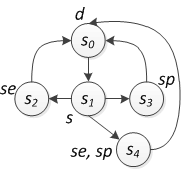
\includegraphics[width=4cm]{NnewCar.png}\\
		\caption{汽车制造企业模型}\label{BVM}
	\end{figure*}

假定,由于经济危机或者战略调整,导致该企业不能再生产跑车。这意味着所有规范和Kripke结构都不再需要考虑$sp$的,因此应该“移除”。
\end{example}

日常生活中也有很多上述例子中的场景,如:商业交易过程、软件开发过程等~\cite{Baier:PMC:2008}。
但是对于给定原子命题集,\emph{从这些大型系统(或规范)中“移除”一些原子命题,而保留与这些原子命题无关的性质是一个复杂的问题}。
%此外,在这种情形下,两个重要的概念:最强必要条件(SNC)和最弱充分条件(WSC)问题也随之产生,其中SNC是指最一般的结论,WSC指最特殊的诱因。

%基于上述存在的问题,下面给出一些解决方案及其意义所在。


\subsection{研究意义}
最强后件(the strongest post-condition,SP)和最弱前件(WP)(分别对应于上文提到的SNC和WSC)是形式化验证中两个重要的概念,其不仅被用于汇编语言程序推理~\cite{legato2002weakest}和制定验证条件\cite{DBLP:journals/ipl/Leino05},还被应用于形式化验证过程中的负例生成\cite{dailler2018instrumenting}和系统精化(refinement)\cite{woodcock1990refinement}。
当模型$\Hm$不满足规范$\varphi$($\Hm\not \models \varphi$)时,找到某个性质$\psi$,使得若$\Hm$按照此性质进行修改后得到的新模型$\Hm'$能满足$\varphi$是必要的,即$\psi$是使得$\Hm\models \varphi$成立的充分条件($\Hm \models \psi\rto \varphi$)。
然而,现有方法不能直接应用于如下情形:计算当$\Hm$为不终止系统(如:反应式系统(reactive system))时使得“$\Hm\models \varphi$”为真的最强必要条件和最弱充分条件
(其详细原因将在下文指出)。此时,\emph{探索如何计算“在$\Hm$下,使得$\varphi$满足的定义在某个符号集合上的SNC和WSC”将更进一步完善模型检测问题,
同时也为基于WSC的负例生成和精化提供了理论依据和新的计算方法。}

本文将探索一种称为\emph{遗忘}(forgetting)的方法来计算充分(必要)条件。如下问所说,遗忘理论作为知识表示与推理(KR)中的重要理论,具有较长的科研历史,且在许多逻辑中都有了较为成熟的研究。然而,在时序逻辑方面的研究目前还不成熟。因此,\emph{本文的研究将为时序逻辑下遗忘理论的研究提供一个理论框架。
与此同时,借助遗忘计算上述形式化验证问题中的充分(必要)条件,架起了KR与形式化验证的桥梁。}

\section{相关研究工作回顾}
\emph{遗忘}是一种重要的知识抽取工具,它具有均匀插值(uniform interpolation)和二阶量化消解(second-order quantifier elimination,SOQE)两种称谓。
在很长一段时间内,遗忘被用于描述逻辑中本体(ontology)摘要的提取、敏感信息的隐藏和软件工程中计算两个文件的逻辑差(logical differences)。此外,其也被用于包括信念更新(belief update)、修改(repair)、规划(planning)和知识独立性的其它领域。

{\em 反应式系统}是一种不终止的、与环境有着持续不断交互的系统,其应用广泛、种类繁多。本文探究如何使用遗忘计算反应式系统下的SNC(WSC),下面就与本文密切相关的反应式系统、遗忘理论和SNC(WSC)进行回顾。

%在规划中,遗忘主要用来计算其对应的后继状态公里所需要的SNC和WSC。下面就与本文密切相关的遗忘理论和SNC(WSC)进行详细的回顾。


\subsection{反应式系统}
随着应用程序在各个领域的应用,对其需求已经发生了重大变化,继而引起模式变化。
以前,一个大型应用程序的运行通常需要数十台服务器,这么高昂的代价换来的是效果和维护成本不成正比:秒级的响应时间,需要数小时的维护。
当前,移动和云端技术的成熟使应用程序不拘泥于以前的方式,它们可以被部署到移动设备和具有多核心处理器的云端集群上。
但是,用户对应用程序的响应时间要求从秒级变到毫秒级,相应的成功率要求为100\%;程序需要处理的数据量也从之前的GB级扩展到现在的PB级。
原有的软件架构已经无法满足当前的需求。

在这种背景下,应用程序需要具备以下特质:即时响应性(Responsive)、回弹性(Resilient)、弹性(Elastic)以及消息驱动(Message Driven)\footnote{https://www.reactivemanifesto.org/zh-CN}。
反应式系统是一种与环境有着持续不断交互的系统,具有不终止的性质~\cite{DBLP:series/txtcs/Schneider04}。此外,其同时满足上述几种要求,且从传统的静态模式逐步向动态、开放、自适应、服务化的模式演化~\cite{jian2012}。
反应式系统由来已久~\cite{DBLP:conf/nato/HarelP84,DBLP:books/sp/trends86/Pnueli86},且种类繁多,如微处理器(microprocessor)、计算机操作系统(computer operating systems),航空交通管制系统(air traffic control systems)、车载电子设备(on-board avionics)以及其它嵌入式系统。

此外,反应式系统的应用非常广泛:包括航空电子等安全攸关的领域和生活息息相关的汽车电子等领域。
安全攸关反应式系统的核心要求是:必须在指定时间期限内完成对外部事件的检测和目标事件的响应,否则会产生灾难性的后果~\cite{wangjuan2019}。
为了确保反应式系统的正确性和实时性,研究者们提出了不同的解决方法,包括:模型检测方法~\cite{DBLP:books/daglib/0007403,clarke1996model,DBLP:series/txtcs/Schneider04}、目标驱动的运行时需求建模框架~\cite{jian2012}、基于图模型的实时规则调度方法(graph-based real-time rule scheduling,简称GBRRS)~\cite{wangjuan2019}、SPARDL~\cite{wangzhen2012}和选择性测试方法~\cite{lishu2004}等。
%这些应用的核心为嵌入式周期控制系统(一种反应式系统),该系统的行为不仅与自身的定义和状态有关,还与控制软件所处的环境有关。
%\begin{itemize}
%	\item 即时响应性:只要有可能, 系统就会及时地做出响应。
%\end{itemize}

在上面的方法中,多数是验证(检测)给定的系统是否具有某种性质。而当系统不满足该性质时,对如何寻找可靠的信息(称为充分条件)来对系统进行修改至关重要。
反应式系统是一种不终止的系统,通常被看作一个Kripke结构。基于此,本文探索如何计算该充分条件,使得系统在该条件下满足给定的性质。




\subsection{遗忘理论}\label{chapter01:forgetting}
遗忘这一词源于Lin等人关于一阶逻辑(first-order logic, FOL)的工作~\cite{lin1994forget},在此之前的研究中多提到的是均匀插值~\cite{visser1996uniform,konev2009forgetting}和SOQE~\cite{ackermann1935untersuchungen}。

在命题逻辑中(propositional logic,PL),公式$\varphi$遗忘一个原子命题$p$,通常记为$\Forget(\varphi,\{p\})$,得到的结果为$\varphi[p/\bot] \vee \varphi[p/\top]$(其与$\exists p\varphi$等价),其中$\varphi[X/Y]$为将$\varphi$ 中 $X$的全部出现替换为$Y$得到的结果。
%在Lin等人的文章中也将$\varphi[p/\bot] \vee \varphi[p/\top]$用$\exists p\varphi$来表示~\cite{lin1994forget}。
公式$\varphi$中遗忘有限原子命题集$P$的定义如下:
\begin{alignat*}{2}
	&  \Forget(\varphi, \emptyset) = \varphi, \qquad \\ % \nonumber
	&  \Forget(\varphi, P \cup \{q\})  = \Forget(\Forget(\varphi, \{q\}), P).
	\nonumber
\end{alignat*}

在FOL中,遗忘通常被看作SOQE问题的一个实例:从FOL公式$\varphi$中遗忘一个$n$-元谓词$P$,得到的结果为一个二阶公式$\exists R \varphi[P/R]$~\cite{lin1994forget},其中$R$为$n$-元变量。
从这个角度看来,遗忘就是找到一个与二阶公式$\exists R \varphi[P/R]$等价的一阶公式。
然而,二阶逻辑的表达能力严格大于一阶逻辑,因而可以容易得出FOL下的遗忘不是封闭(存在)的结论,也就是从某些一阶公式中遗忘某些谓词得到的结果不可以用一阶公式来表示。
作为FOL的一个子类,描述逻辑公式的遗忘也不总是存在的~\cite{DBLP:journals/ai/KonevL0W13},甚至对最基本的描述逻辑{\cal ALC}而言,遗忘的存在性问题都是不可判定的。
尽管如此,描述逻辑作为一种在语义网领域很重要的语言,其子类中的遗忘通常被用来抽取视图(review)~\cite{Wang:AMAI:2010,DBLP:conf/ijcai/LutzW11,Konev:JAIR:2012,DBLP:conf/ijcai/ZhaoS17,DBLP:conf/aaai/ZhaoSWZF20}。这些子类包括:ALCOI(the basic ALC extended with nominals and inverse roles)和ALCOIH(ALCOI extended with role hierarchies, the universal role and role conjunction)。%textcolor{red}{(包括{\cal ALCOHI}和{\cal ALCOIH})}

现有计算一阶逻辑和描述逻辑遗忘的方法有基于归结(resolution)和基于Ackerm- ann引理的方法~\cite{DBLP:books/daglib/0023036}。
其中基于归结的方法是一种基于子句归结的方法,其基础是归结规则。通常在这种方法中首先把公式转换为其子句形式,然后使用归结规则,最后移除含有要遗忘的谓词(原子命题)的子句,得到的结果可能就为遗忘的结果(在后文中会详细介绍与本文相关的归结规则和转换规则)。
基于Ackermman引理的方法主要是直接或间接(扩展)使用下面的Ackermann引理得到的。
\begin{lemma}[引理 6.1~\cite{DBLP:books/daglib/0023036}]
	给定关系变元$X$和一阶公式$\alpha(\overline{x}, \overline{z})$和$\beta(X)$,其中$\overline{x}$和$\overline{z}$为普通变元构成的多元组、$\overline{x}$中变元的个数与$X$的参数个数相同、且$\alpha$中不包括$X$。
	\begin{itemize}
		\item 若$\beta(X)$关于$X$是正的,即:$X$在$\beta(X)$中的每次出现前面都有偶数个“$\neg$”符号,则:
		$$\exists X \{\forall \overline{x} [X(\overline{x}) \rto \alpha(\overline{x},\overline{z})] \wedge \beta(X)\} \equiv \beta(X)_{\alpha(\overline{x},\overline{z})}^{X(\overline{x})}\hbox{。}$$
		\item 若$\beta(X)$关于$X$是负的,即:$X$在$\beta(X)$中的每次出现前面都有奇数个“$\neg$”符号,则:
		$$\exists X \{\forall \overline{x} [ \alpha(\overline{x},\overline{z}) \rto X(\overline{x})] \wedge \beta(X)\} \equiv \beta(X)_{\alpha(\overline{x},\overline{z})}^{X(\overline{x})}\hbox{。}$$
	\end{itemize}
其中,$\beta(X)_{\alpha(\overline{x},\overline{z})}^{X(\overline{x})}$表示将$\beta(X)$中$X(\overline{x})$的全部出现用$\alpha(\overline{x},\overline{z})$来替换得到的公式。
\end{lemma}



\emph{知识遗忘}(knowledge forgetting)在模态逻辑S5中首先被提出并被用于推理智能体的知识状态(知识或者信念)~\cite{Yan:AIJ:2009}。
因为模态逻辑系统中引入了模态词,模态逻辑中的遗忘不同于经典逻辑下的遗忘。所以,不能以简单的谓词(命题)替换的方式获取遗忘的结果,如:
\begin{example}\cite{Zhang2008Properties}
	令S5公式$\varphi=\MPK p \wedge \neg \MPK q \wedge \neg \MPK \neg q$,则使用命题逻辑下的计算方法得到的结果为$\varphi[q/\top] \vee \varphi[q/\bot] \equiv \bot$。
	这显然是不正确的,因为在遗忘$q$之后智能体的知识库不应该变得不一致。
\end{example}
为此,新的计算方法和四个能精确描述知识遗忘的基本公设被给出,这几个公设为:削弱(weaking)、正支持(positive persistence)、负支持(negative persistence)和无关性(irrelevance)。
%值得注意的是这四个条件与知识遗忘形成了“当且仅当”的关系。换句话说,当知道某一个公式满足那四个条件则该公式为遗忘的结果,当知道某一结果为遗忘结果时它一定满足那四个基本条件。
此外,模态谓词逻辑下信息不完备的知识遗忘~\cite{wenximing2019buwanbei}、模态一阶逻辑S5中的遗忘也得到了研究~\cite{Yongmei:IJCAI:2011},Fang等人讨论了关于多模态(multi-modal)$K_n$、 $D_n$、 $T_n$、$K45_n$、 $KD45_n$情形下遗忘的存在性~\cite{DBLP:journals/ai/FangLD19,wenximing2019,wenximing2019kn}——这些逻辑里的遗忘总是存在的,其中$n$为智能体的个数。


均匀插值作为遗忘的一个对偶概念。
从形式上说,如果一个逻辑系统${\cal L}$中任意的公式$\varphi$和$\psi$,若$\varphi\models_{\cal L} \psi$,则存在一个公式$\xi$使得$\varphi\vdash_{\cal L}\xi$、$\xi\vdash_{\cal L}\psi$和 $\Var(\xi)\subseteq \Var(\varphi)\cap \Var(\psi)$,
则${\cal L}$具有或Craig插值性质,若$\xi$与$\psi$无关,则${\cal L}$具有均匀插值性质。

其在模态逻辑和时序逻辑系统中取得了一系列研究成果:LTL、$\CTL$和$\CTL^*$不具有均匀插值性质~\cite{Maksimova:JANCL:1991,DAgostino:synthese:2008},
S5、K和KD模态逻辑系统具有均匀插值性质~\cite{DBLP:journals/aml/Iemhoff19},
而一些模态逻辑系统没有均匀插值性质。如:量词模态逻辑S5(quantified modal logic S5)\cite{DBLP:journals/jsyml/Fine79}、K4、和S4及其扩展都没有均匀插值性质~\cite{DBLP:journals/ndjfl/Schumm86},因而其遗忘也不是封闭的。
研究具有均匀插值性质的模态逻辑遗忘可以借鉴S5系统的遗忘方法,也可以参考K系统下基于归结计算均匀插值的方法。
对于那些没有均匀插值的模态逻辑系统,可以考虑模态逻辑下的Ackermann引理~\cite{DBLP:books/daglib/0023036}。



%此外,Feng等人也研究了S5下如

在非单调推理(non-monotonic reasoning)环境中,科研工作者们也从遗忘需要满足的基本条件的视角研究了
基于回答集语义的逻辑程序的遗忘,这些工作包括Zhang、Wang等人发表在AI、AAAI和JAIR上的文章~\cite{DBLP:Zhang:AIJ2006,DBLP:journals/ai/EiterW08,Wong:PhD:Thesis,DBLP:journals/jair/WangZZZ14,wang2013forgetting,DBLP:conf/aaai/WangWWZ15,DBLP:journals/jair/Delgrande17,gonccalves2020limits},和Eiter、Gonccalves等人的综述~\cite{eiter2019brief,gonccalves2021forgetting}。


%应用
遗忘有很多应用,这里列出下面几点:
\begin{itemize}
	\item 计算后继状态公理:在规划问题中,根据最强必要条件和最弱充分条件有利于求出后继状态公理\cite{DBLP:journals/jair/Lin03}。%在该文章中,最强必要条件和最弱充分条件都用遗忘来计算;
	\item 信息隐藏:在某些关键领域,为实现隐私保护,必须隐藏敏感信息。现有方法包括基于本体\cite{DBLP:journals/ai/KonevL0W13}和基于DataSecOps的个人信息保护\cite{wangwen2021}。要做到隐私保护,只需要隐藏(遗忘)那些敏感的概念(concept)和角色(role)符号。值得注意的是,个人信息保护涉及被遗忘权\cite{zhujia2020};
%	\item 计算逻辑差:
	\item 知识更新:在许多场景,知识不是一层不变的,随着时间或空间的推移,会有新的知识加入。如何用新加入的信息更新原有知识,而保证知识库的一致性是知识更新需要解决的问题。此外,知识更新也需要满足一些基本条件。在这些基本条件中,Katsuno和Mendelzon提出的$(U1)$-$(U8)$较为常用;%,本文也使用这几个基本条件;
	\item 提取本体的概要:当一个本体工程师想要快速了解并测试一个本体的内容时,能事先快速地摒弃许多无关信息,并提取出本体的概要是非常有用的;
	\item 知识归并:知识库通常来自于多个信息源,这些分布的信息大多会存在冲突(不一致),因而不能简单地将它们放在一起。归并考虑当这些信息矛盾时如何将它们整合\cite{DBLP:journals/tkde/LiberatoreS98,DBLP:journals/logcom/KoniecznyP02,DBLP:journals/jair/Maynard-ZhangL03,konieczny2004da2,DBLP:journals/ai/EveraereKM10},且基于遗忘的归并可以尽可能少地遗忘原子以保持知识的一致性\cite{xudai2011}。
	\item 逻辑独立性:生活中许多场景都需要判断哪些信息是无关的(或相关的),即信息的独立性\cite{DBLP:journals/jphil/Sandu93,DBLP:journals/igpl/Sandu97,DBLP:journals/igpl/Vaananen02,DBLP:journals/synthese/Sevenster06},如:知识归并中能知道哪些信息是无关的,那么知识归并将变得容易一些。在智能推理中,智能体也需要判断哪些东西(如:命题或文字)是无关的。除了无关性,还有其它名字揭示了这一本质,如:独立性(independence)、非冗余的(irredundancy)、非影响的(influenceability)、分离的(separability)以及交互性(interactivity)。基于遗忘的独立性表明,被遗忘的原子(文字、公式)与得到的结果无关。所以,当遗忘的结果与原公式等价时,该公式与被遗忘的原子(文字、公式)无关\cite{xudai2011}。
%	\item 遗忘在归并和逻辑独立性中也有着重要作用\cite{xudai2011}。
\end{itemize}







\subsection{最强必要条件(SNC)和最弱充分条件(WSC)}


正如上文所说,WSC(SNC)对于软件工程中系统的形式化验证非常重要。
此外,SNC和WSC还可用于系统精化~\cite{woodcock1990refinement}、模型检测中的负例产生~\cite{dailler2018instrumenting}、汇编语言程序的推理~\cite{legato2002weakest}和制定验证条件~\cite{DBLP:journals/ipl/Leino05}。
一般说来,最强必要条件(SNC)是最一般的推论(the most general consequence),即:命题成立时能推出的最强后件(SP),SNC能够蕴涵所有的必要条件;最弱充分条件(WSC)是最特殊的诱因(the most specific abduction),即:使得命题成立的最弱前提条件(WP),WSC能被所有的充分条件蕴涵。

给定一个程序(program)$S$和某一状态(state)的规范(specification)$Q$,若$S$关于$Q$的WSC是一个能够描述$S$初始状态的规范,那么前提是$S$满足以下两个条件:

(i)$S$必须终止,

(ii)$S$执行完成后必须到达能满足$Q$的状态。\\
%\begin{itemize}
%	\item[(i)] $S$必须终止,
%	\item[(ii)] $S$执行完成后必须到达能满足$Q$的状态。
%\end{itemize}
Dijkstra提出了四条规则来计算这样的规范,程序语言里的四种语句(即:赋值语句(assignment statement)、顺序语句(sequence statement)、条件语句(conditional statement)和循环语句(loop statement))分别对应了这四种规则~\cite{DBLP:journals/cacm/Dijkstra75}。
在上述计算WSC的方法中,有一个必须满足的要求是“$S$必须终止”。这就是上文中说到的当系统为反应式系统这类不终止系统时,现有方法不能计算WSC的主要原因。



在知识表示与推理中,SNC和WSC为因果理论中后继状态公理的计算提供了一种方法~\cite{DBLP:journals/jair/Lin03},且SNC和WSC都可以用遗忘来计算~\cite{DBLP:journals/ai/Lin01,DBLP:conf/ijcai/DohertyLS01}。
随后,SNC和WSC被扩展到FOL下,且用SOQE实现了SNC和WSC的计算~\cite{DBLP:conf/ijcai/DohertyLS01}。

本文将在背景知识部分对SNC和WSC在命题逻辑和模态逻辑这两种情形进行详细介绍(包括其定义和算法)。






\section{研究目标及主要结果}

相关研究工作表明,现存方法不能求解反应式系统下的WSC(SNC)。然而,WSC是一种进行系统修改的重要知识,寻求一种有效的求解方法有利于确保系统的正确性。
在知识表示与推理中,遗忘技术可以用于计算给定理论(公式)的WSC(SNC)。
但是,如上所述,时序逻辑下的遗忘理论尚处于不成熟阶段,没有一个统一的理论框架。
此外,如何用遗忘来计算给定系统模型和性质的WSC(SNC)也是一个重要问题。

基于此,{\em 本文从遗忘理论的角度出发,研究反应式系统下SNC和WSC的计算方法,从而为计算不终止类系统下定义在某个符号集上的SNC和WSC提供了新的方法,架起形式化验证与KR之间的桥梁。}
%特别地,本文将规范的描述语言限制到$\CTL$和$\mu$-演算下。
为了实现这一目标,本文\textbf{主要研究内容及结果}如下:

(1) {\em $\CTL$和$\mu$-演算的遗忘理论}

本文探究了$\CTL$和$\mu$-演算中遗忘的定义和性质,特别是其遗忘结果的存在性、复杂性等,为探索用遗忘计算SNC和WSC奠定理论基础。具体说来,遗忘具有削弱、正维持、负维持 、无关性等基本准则\cite{Yan:AIJ:2009}。本文探索$\CTL$和$\mu$-演算遗忘的以上四个准则,并探讨其与存在性之间的关系。此外,本文研究了 $\CTL$和$\mu$-演算 中计算遗忘结果的方法,探讨了$\CTL$和$\mu$-演算遗忘相关问题的复杂性结果,为研究计算SNC和WSC的性质、算法以及基本准则等作铺垫。具体说来,有以下两点:
\begin{itemize}
	\item \textbf{$\CTL$的遗忘理论:}
	$\CTL$不具有Crig插值(Crig interpolation)性质,因而不具有均匀插值(uniform interpolation) 性质\cite{Maksimova:JANCL:1991},即:存在一个两个公式$\varphi$和$\psi$,若$\varphi \models \psi$,不存在由$\varphi$和$\psi$的公共元素构成的公式$\theta$,使得$\varphi \models \theta$且$\theta \models \psi$。
%	即:不存在一个算法使得对于任意的$\CTL$公式,其“遗忘”掉任意原子命题的集合得到的结果仍然是$\CTL$公式。
	在这种情况下,本文除了研究上述$\CTL$遗忘的性质,还针对$\CTL$子类,特别是能保证其遗忘结果仍然是$\CTL$可表达的子类的遗忘进行了研究。在这些子类中,一个特殊的子类是约束$\CTL$(bunded \CTL):每个公式具有有限个模型,且每一个模型都能用一个$\CTL$公式表达。因此,其遗忘是封闭的。
	
	\item \textbf{$\mu$-演算的遗忘理论:}
	与$\CTL$不同,$\mu$-演算虽然表达能力比$\CTL$强,其可满足性问题也比$\CTL$的复杂,但是$\mu$-演算具有均匀插值性质\cite{d2006modal}。这意味着,$\mu$-句子遗忘任意原子命题集得到的结果仍然是$\mu$-句子。本文给出了$\mu$-演算下遗忘的主要框架:包括上述遗忘的性质和计算遗忘的方法。
	与$\CTL$不同,$\mu$-演算公式含有变元。为此,本文提出一种新的互模拟,并证明$\mu$-公式对这种互模拟是不变的(invariant)。
	特别地,证明了$\mu$-演算遗忘与均匀插值是一个对偶概念,这为研究均匀插值提供了另一种途径。
	此外,本文还证明了当$\mu$-公式为析取$\mu$-公式时,计算遗忘可以在多项式时间内完成,这为$\mu$-演算遗忘的计算提供了一种有效的方法。
\end{itemize}


(2) {\em 计算$CTL$遗忘的算法}

基于上述研究结果,设计并使用Prolog实现了计算$\CTL$遗忘结果的原型系统,并从理论和实验角度分析其计算复杂性。
%具体说来,给出了一种基于归结的计算$\CTL$遗忘的算法,并使用Prolog实现了该算法。
此外,对于约束$\CTL$的情形,本文也提出了一种基于模型的算法。

(3) {\em 遗忘理论在反应式系统的形式化验证和知识更新中的应用}

反应式系统用Kripke结构表示,Kripke结构是公式的模型。因而,基于上述研究,
给出了基于遗忘的计算“有限系统模型(Kripke结构)在给定条件下的SNC和WSC”的方法。
%给出了使用遗忘计算有限系统模型(Kripke结构)在给定条件下SNC和WSC的方法。
如上所述,一个有限的系统模型能够被一个$\CTL$公式描述,遗忘可以看作以公式和原子命题为运算对象的函数,因而可以使用遗忘计算该系统的SNC和WSC。
此外,知识更新是一种使用新发现的性质更新已有理论的技术。本文探讨了如何使用遗忘更新$\CTL$和$\mu$-演算表达的知识;
表明了使用遗忘定义的知识更新满足现有的知识更新的八条准则。

~\\
针对上述几个内容,解决了以下3个\textbf{关键问题}:

(1) {\em $\CTL$的遗忘什么情形下存在?如何计算遗忘?}

$\CTL$是一种分支时序逻辑,其引入了时序算子,已有文献表明$\CTL$不具有均匀插值性质。因为遗忘与均匀插值是一对对偶概念,研究$\CTL$的遗忘不能像已有的经典命题逻辑和模态逻辑S5那样。为此,本文深度剖析现存的归结规则,提出了一种基于归结的计算遗忘的方法,并证明:当所有在转换为$\CTL$标准形式过程中引入的新原子命题都被“消除”时,使用这一方法得到的结果即为遗忘结果。
尽管$\CTL$遗忘不是封闭的,但本文给出:当被归结的原子命题只同时出现在同一模态词下的命题公式里时,遗忘总是存在的。

此外,针对约束$\CTL$的遗忘,证明了其遗忘结果可以由有限个模型的特征公式(一种$\CTL$公式)的析取来表示,所以这种情形下的遗忘是封闭的。

(2) {\em 遗忘理论与反应式系统的SNC和WSC的关系}

在经典命题逻辑和一阶逻辑中,Lin 和 Doherty 等人分别提出了遗忘与SNC(WSC)的关系~\cite{DBLP:journals/ai/Lin01,DBLP:conf/ijcai/DohertyLS01}。特别地,经典命题逻辑中的SNC和WSC被用于计算规划问题中的后继状态公理。本文给出,给定一个有限反应式系统(Kripke structure),并将该系统表示为其特征公式,就可使用
上述的$\CTL$和$\mu$-演算遗忘计算SNC和WSC。



(3) {\em $CTL$和$\mu$-演算的遗忘在推理问题上的复杂性}

计算复杂性理论致力于将可计算问题根据它们本身的复杂性分类。研究表明,在经典命题逻辑中:CNF(Conjunctive normal form)公式遗忘的推理问题最难是$\Pi_2^P$-完全的,DNF (Disjunctive normal form)公式遗忘的蕴涵问题是co-NP-完全的。在命题模态逻辑S5中,遗忘的模型检测问题是NP-完全的,对应的蕴涵问题是$\Pi_2^P$-完全的。本文从现有复杂性结果和自动机理论基础上研究$\CTL$和$\mu$-演算遗忘在推理问题上的复杂性。
研究表明,$\mu$-演算下关于遗忘的模型检测是$\textsc{Exptime}$的,蕴涵问题都在$\textsc{Exptime}$中,且有的蕴含问题是$\textsc{Exptime}$-完全的。
$\CTL$下关于遗忘的推理问题:当只考虑特殊段$\CTL_{\ALL \FUTURE}$(公式中只包括时态算子$\ALL \FUTURE$)时,其模型检测的复杂性为\textsc{NP}-完全的;而蕴涵问题的复杂性在co-$\textsc{NP}$-完全的和$\Pi_2^{\textsc{P}}$-完全的之间。








\section{论文组织结构}
本文研究了计算树逻辑和$\mu$-演算下的遗忘理论,并探讨如何使用遗忘技术来计算SNC(WSC)和知识更新。全文共分为九章,组织结构如图\ref{fig:chapter1-research-structure}所示,各章节内容的具体安排如下:


\begin{figure}[htbp]
	\centering
	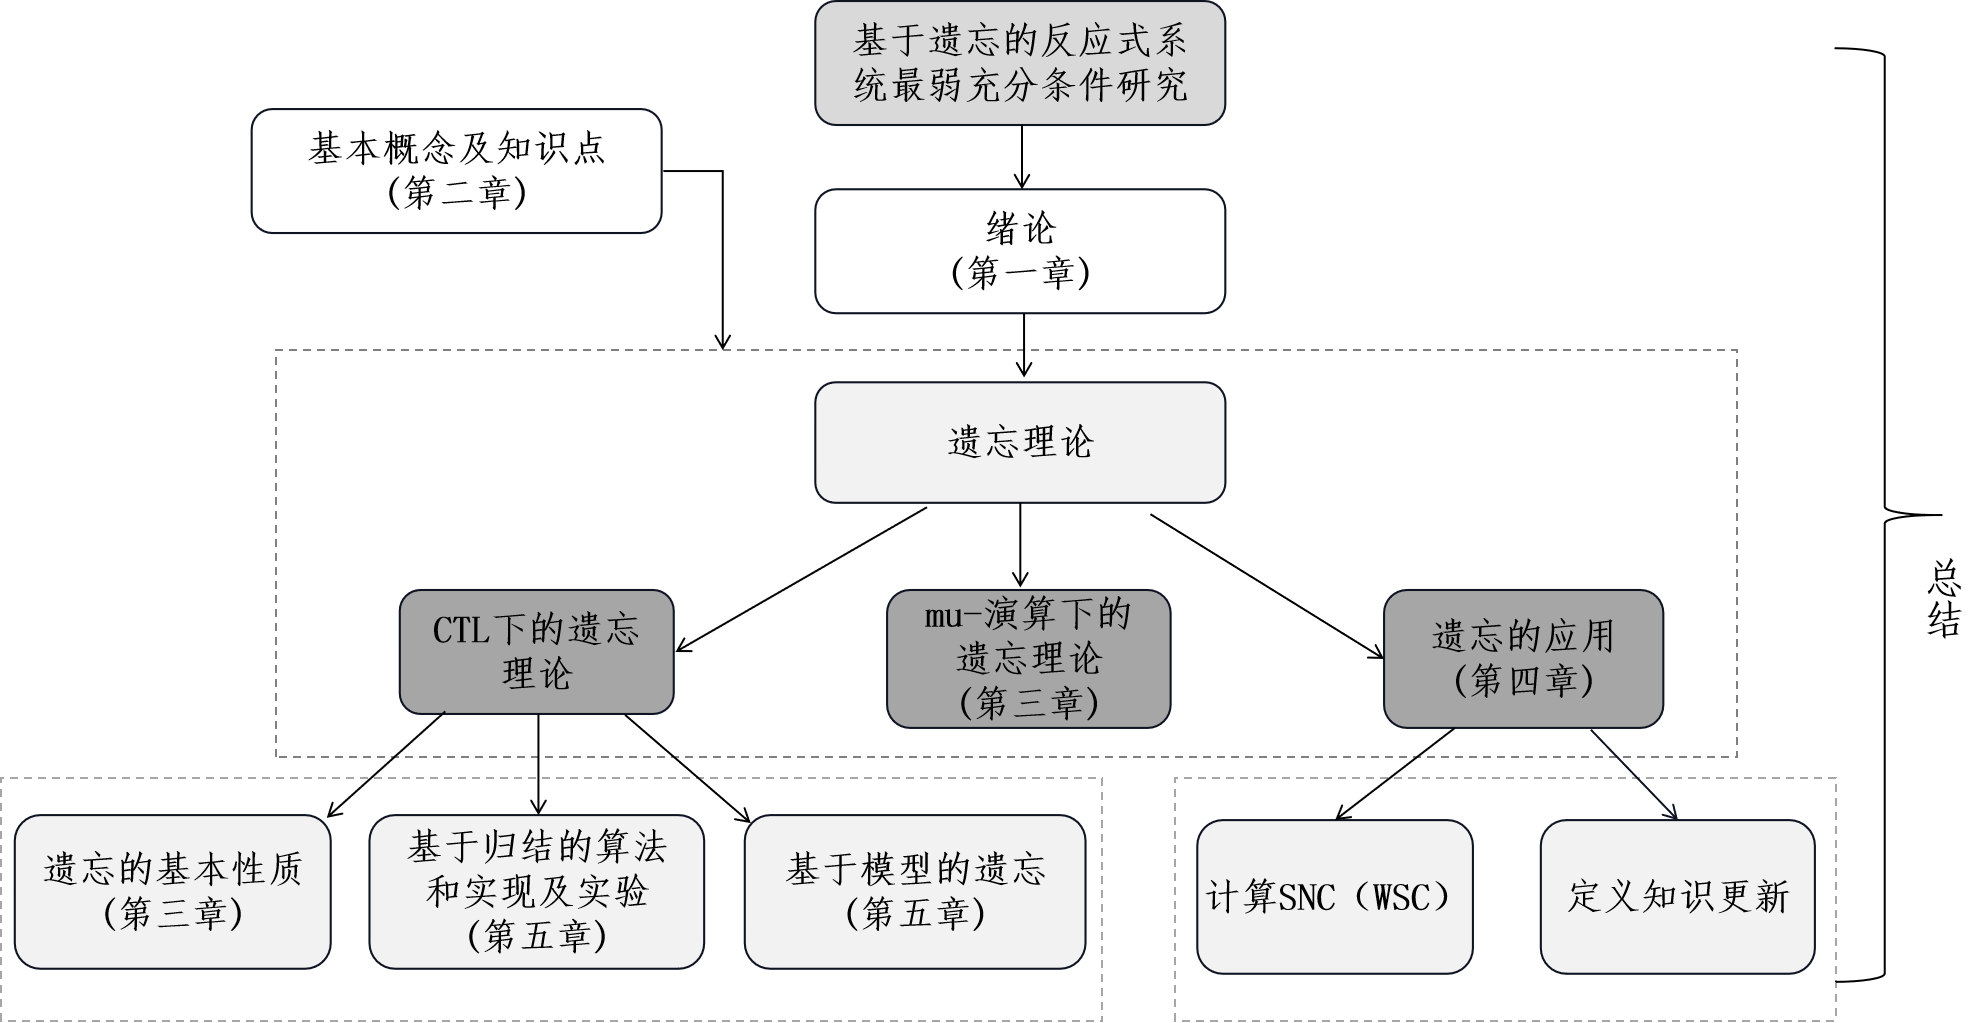
\includegraphics[width = 1\linewidth]{chapter01/zuzhi.png}
	\caption{本文的章节内容组织结构图}
	\label{fig:chapter1-research-structure}
\end{figure}

第\ref{chapter01}章为\textit{绪论},首先阐述了本文的研究背景及意义,并分析给出了存在的问题,凝练出本文研究需要解决的关键问题。基于上述分析,阐述了本文的研究内容和研究取得的主要成果。最后给出了本文的章节组织结构安排。


第\ref{chapter02}章为 {\em 背景知识},介绍了本文研究所涉及逻辑语言的语法语义及相关技术。首先,给出了经典命题逻辑下解释(赋值)的定义,以及相关语言的模型结构——Kripke结构。
然后,本章给出$\CTL$和$\mu$-演算的语法和语义。
最后,除了最强必要条件和最弱充分条件在经典逻辑和模态逻辑S5下的研究,本章还介绍了与上述逻辑语言密切相关的两个技术:遗忘和$\CTL$下的归结。



第\ref{chapter03}章 {\em 给出$\CTL$和$\mu$-演算遗忘的定义及其基本性质}。首先,给出一种新的互模拟定义,并介绍其基本属性;其次,使用互模拟来定义$\CTL$和$\mu$-演算下的遗忘,并研究遗忘的属性,包括表达性属性(representation theory)和复杂性结果等。本章指出$\CTL$遗忘是不封闭的,即存在某些公式的遗忘结果不能用$\CTL$来表示。此外,证明了$\mu$-句子遗忘的结果总是存在的,且不含有不动点操作的这类$\mu$-公式遗忘的结果总在这个类里面。

第\ref{chapter04}章 为{\em 遗忘理论在反应式系统中的应用}。讲述如何将遗忘应用于计算反应式系统在给定条件下的SNC(WSC)和定义知识更新。
此时,有限状态的反应式系统模型的WSC(SNC)可以通过遗忘来计算,且通过遗忘定义的知识更新满足Katsuno等人提出的八条基本准则。


第\ref{chapter05}章 为{\em $\CTL$遗忘的计算方法}。讲述了两种计算$\CTL$遗忘的方法:基于模型和基于归结的方法。此外,给出了基于归结的算法Prolog实现描述和实验结果分析。
在基于模型的计算$\CTL$遗忘中:第~\ref{chapter05:sec:model}节探讨了约束$\CTL$遗忘是封闭的情形;为此,提出了一种约束的互模拟,并定义给定深度的计算树在给定原子命题集下的特征公式,继而给出有限情况下Kripke结构在给定原子命题集下的特征公式;最后说明,在约束情形下,$\CTL$公式的遗忘结果总是$\CTL$公式可表达的。
在基于归结的计算$\CTL$遗忘中:首先,将$\CTL$公式转换为归结规则需要的子句形式——$\CTLsnf$子句;其次,使用归结规则计算要遗忘的原子命题上所有可能的归结结果;随后,移除那些含有要遗忘的原子命题的子句,并给出一种一般化的Ackermann引理消除一些新引入的原子命题;最后,将得到的结果转换成$\CTL$公式。此外,根据上述过程,提出计算$\CTL$遗忘的算法,并分析该算法的时间和空间复杂性。


%第\ref{chapter04}章 为{\em 基于归结的$\CTL$遗忘计算}。基于第\ref{chapter02}章的归结规则,本章探讨如何使用该归结系统计算$\CTL$下的遗忘。首先,将$\CTL$公式转换为归结规则需要的子句形式——$\CTLsnf$子句(后文详细介绍);其次,使用归结规则计算所有可能的需要遗忘的原子命题上的归结结果;随后,移除那些包含要遗忘的原子命题的子句,并给出一种一般化的Ackermann引理消除一些新引入的原子命题;最后,将得到的结果转换成$\CTL$公式。此外,基于上述过程提出计算$\CTL$下的遗忘的算法,并分析该算法的时间和空间复杂性。

%第\ref{chapter05}章 为{\em 约束$\CTL$下的遗忘}。在第\ref{chapter03}章所说,$\CTL$下的遗忘不是封闭的,因此在本章探讨了约束$\CTL$遗忘是封闭的情形。为此,本章提出了一种约束的互模拟,并给出给定深度的计算树在给定原子命题集合下的特征公式,继而给出有限情况下Kripke结构在给定原子命题集合下的特征公式。最后说明约束情形下$\CTL$公式的遗忘结果总是$\CTL$公式可表达的。




%第\ref{chapter06}章 为{\em $\mu$-演算下的遗忘}。$\mu$-演算是一种表达能力比$\CTL$强的时序逻辑,其具有均匀插值性质。本章给出$\mu$-演算下遗忘的定义和基本属性,包括模块性、交换性及同质性。此外,探讨了$\mu$-演算下的遗忘是封闭的,且对任意析取$\mu$-公式的遗忘可以在多项式时间内计算出来。
%最后,给出$\mu$-演算下关于遗忘算子的模型检测和推理问题的复杂性结果。



%第\ref{chapter07}章 为\textit{遗忘理论的应用}。讲述如何将遗忘应用于计算SNC(WSC)和定义知识更新。
%此时,有限状态的反应式系统模型的WSC(SNC)可以通过遗忘来计算,且通过遗忘定义的知识更新满足Katsuno等人提出的知识更新应该满足的基本准则。
%在这种情形下将公式的模型限制到有限状态空间,组成公式的原子命题也是有限的。经过

%第\ref{chapter08}章 为\textit{实验结果}。给出基于归结的算法实现模型的实验结果及分析。


第\ref{chapter09}章为\textit{总结与展望}。首先总结了本文的研究工作,进一步,展望了未来研究工作的方向和重点。
%绪论

\chapter{Kripke结构、时序逻辑、模型检测以及遗忘理论}\label{chapter02}

{\em 本章主要介绍本文用到的符号、术语以及逻辑理论基础,包括:Kripke结构、时序逻辑(尤其是计算树逻辑(CTL)和$\mu$-演算)、模型检测和遗忘理论。首先,介绍解释时序逻辑语言所需的模型结构,即Kripke结构。其次,主要介绍时序逻辑中本文探讨的计算树逻辑和$\mu$-演算。为了更加明确本文的研究动机,本章将详细介绍模型检测的基本概念和一些主要的性质。此外,遗忘理论是本文的研究重点,其概念、性质及在各个研究领域的研究和应用情况将会被当作本章的重点详细介绍。

为了方便,本文将命题变量(也叫原子命题)的集合记作$\cal A$,$V\subseteq {\cal A}$ 是$\cal A$的子集。此为,规定$\overline{V}$是$V$在${\cal A}$上的补,也即是$\overline{V}={\cal A}-V$。}
%{\em 围绕差分隐私应用中存在的隐私与数据可用性之间的权衡问题,本文以隐私信息度量为基础,试图从均衡优化的角度提供一种解决方案。为了更好的阐述后续的研究内容,本章首先介绍本文工作所需的基本模型与定义,包括隐私定义、差分隐私模型的形式化定义、Shannon信息论的基本通信模型及信息熵的概念。随后,介绍信息论、优化理论与对策博弈的基础知识,并以此为基础介绍了差分隐私均衡优化主要研究问题的描述及定义。本章阐述的内容主要为后续章节的具体研究奠定基础。}

\section{Kripke结构}
Kripke结构作为一种表示转换系统(transition system)的数学模型,在理论计算机科学领域有着广泛的应用,尤其是作为解释时序逻辑公式的模型结构。

\subsection{真假赋值和K-解释}
经典命题语言${\cal L}^p$由以下三类符号构成:
\begin{itemize}
	\item 命题符号:一般用小写拉丁字母$p$,$q$,$r$,$\dots$来表示,且这些命题符号来源于$\Ha$;
	\item 联结符号:$\neg$(否定),$\wedge$(合取),$\vee$(吸取),$\rto$(蕴涵),$\lrto$(等值于);
	\item 标点符号:((左括号),)(右括号)。
\end{itemize}
%命题符号:一般用小写拉丁字母$p$,$q$,$r$,$\dots$来表示,且这些命题符号来源于$\Ha$;
%连接符号:$\neg$(否定),$\wedge$(合取),$\vee$(吸取),$\rto$(蕴涵),$\lrto$(等值于);
%标点符号:((左括号),)(右括号)。

${\cal L}^p$的原子公式的集合和公式的集合分别记作$Atom({\cal L}^p)$和${\cal F}({\cal L}^p)$。其中,$Atom({\cal L}^p)$是命题符号的集合,且$\varphi\in {\cal F}({\cal L}^p)$当且仅当它能由(有限次使用)以下的三条规则生成\cite{luzhongwan1989}:
\begin{itemize}
	\item 如果$\varphi\in Atom({\cal L}^p)$,则$\varphi \in {\cal F}({\cal L}^p)$。
	\item 如果$\varphi \in {\cal F}({\cal L}^p)$,则$(\neg \varphi)\in {\cal F}({\cal L}^p)$。
	\item 如果$\varphi$,$\varphi'\in {\cal F}({\cal L}^p)$,则$(\varphi * \varphi')\in {\cal F}({\cal L}^p)$。其中,$*\in \{\wedge,\vee, \rto, \lrto\}$。
\end{itemize}
此外,也称“ture”和“false”为原子公式,分别记为“$\top$”和“$\bot$”。原子命题或其否定称为\emph{文字},有限个文字的吸取称为\emph{子句}。

\begin{example}\label{exp:pro:form}
	下面几个字符串为${\cal L}^p$的公式:
	\begin{itemize}
		\item $(q \vee p)$;
		\item $(((\neg p)\lrto(q\vee r))\rto(r \wedge p))$。
	\end{itemize}
	而字符串$p\wedge \vee q$不属于集合$\varphi\in {\cal F}({\cal L}^p)$。
\end{example}


为了方便,称${\cal L}^p$的公式为\emph{命题公式}(在不引起歧义的情况下也称之为\emph{公式})。此外,规定联结符号的优先级有助于简化公式(省略掉冗余的标点符号)。为此,规定在下面的序列中,每个左边的联结符号优先于右边的联结符号。
\[
\neg \qquad \wedge \qquad \vee \qquad \rto \qquad \lrto
\]
此时,例~\ref{exp:pro:form}中的公式$(((\neg p)\lrto(q\vee r))\rto(r \wedge p))$就可写为$(\neg p \lrto q \vee r) \rto r \wedge p$。当然,为了看起来方便,有的括号可以不必省略。

在讨论了命题公式的语法结构之后,接下来将讨论其语义解释。

\begin{definition}[真假赋值]\label{def:pro:interp}
	真假赋值是以所有命题符号的集为定义域,以真假值的集$\{0,1\}$为值域的函数$v:{\cal A}\rto \{0,1\}$。
\end{definition}
为了方便,后文中也将$\top$代表$1$,$\bot$代表$0$(此时真假赋值为$v:\Ha \rto \{\bot, \top\}$),且满足对任意的真假赋值$v$都有$\top^v=1$和$\bot^v=0$。由该定义可知,一个真假赋值要同时给${\cal A}$中的所有命题符号指派一个真假值,所以真假赋值的个数为$2^{|{\cal A}|}$。真假赋值$v$给公式$\varphi$指派的值记作$\varphi^v$,可形式化定义为如下:
\begin{definition}[公式的真假值]\label{def:pro:vformula}
	真假赋值$v$给公式指派的真假值递归定义如下:
	\begin{itemize}
		\item $p^v\in \{\bot,\top\}$,其中$p\in\Ha$。
		\item $(\neg \varphi)^v=\left\{
		\begin{array}{ll}
			\top, \qquad \hbox{如果$\varphi^v=\top$;} \\
			\bot,  \qquad  \hbox{否则。}
		\end{array}
		\right.$
		\item $(\varphi \wedge \psi)^v=\left\{
		\begin{array}{ll}
			\top, \qquad \hbox{如果$\varphi^v=\psi^v=\top$;} \\
			\bot,  \qquad  \hbox{否则。}
		\end{array}
		\right.$
		\item $(\varphi \vee \psi)^v=\left\{
		\begin{array}{ll}
			\top, \qquad \hbox{如果$\varphi^v=\top$或$\psi^v=\top$;} \\
			\bot,  \qquad  \hbox{否则。}
		\end{array}
		\right.$
		\item $(\varphi \rto \psi)^v=\left\{
		\begin{array}{ll}
			\top, \qquad \hbox{如果$\varphi^v=\bot$或$\psi^v=\top$;} \\
			\bot,  \qquad  \hbox{否则。}
		\end{array}
		\right.$
		\item $(\varphi \lrto \psi)^v=\left\{
		\begin{array}{ll}
			\top, \qquad \hbox{如果$\varphi^v=\psi^v$;} \\
			\bot,  \qquad  \hbox{否则。}
		\end{array}
		\right.$
	\end{itemize}
\end{definition}
对于任意的命题公式$\varphi$和真假赋值$v$,当$\varphi^v=\top$时,称$v$是公式$\varphi$的一个模型,也可以记为$v \models \varphi$,读作$v$满足$\varphi$。一般地,当存在一个真假赋值$v$使得$v\models \varphi$,则称公式$\varphi$是\emph{可满足的}。如果$\varphi$是可满足的,且$\neg \varphi$是不可满足的,则称$\varphi$是\emph{有效的}。

值得注意的是,命题逻辑的语义也可定义在“解释(interpretation)”上。一个\emph{解释}$I$是$\Ha$的子集。除了对原子命题$p\in \Ha$,$I$对公式的解释如真假赋值一样。在解释原子命题$p\in \Ha$上,$p^I$为真当且仅当$p\in I$。模型和可满足的定义与真假赋值的类似。

模态逻辑是经典逻辑的扩充,它是经典逻辑中引进“必然”和“可能”这两种模态词得到的。如上所述,命题的真假值只有两种,命题是真的(1)或是假的(0)。而在模态逻辑中,把命题
区分为必然真的命题和并非必然真的命题,把假命题区分为必然假的和并非必然假的命题。对于任何命题$\varphi$,可以有两种模态命题:“$\varphi$是必然的”和“$\varphi$是可能的”。值得注意的是,时序逻辑也是模态逻辑的一种\cite{gabbay2008second}。尽管如此,本文在说模态逻辑的时候通常指不带有时序操作符的情况,说时序逻辑时指带有时序操作符的情况。

本文所说的模态逻辑为命题单模态逻辑(propositional mono-modal logic)。模态公式的集合${\cal F}^{\Hm}$是包含“$\top$”和“$\bot$”的满足如下条件的最小集:
\begin{itemize}
	\item $\Ha \subseteq {\cal F}^{\Hm}$;
	\item 如果$\varphi \in {\cal F}^{\Hm}$,则$(\neg \varphi)$,$(\MPK \varphi)\in {\cal F}^{\Hm}$;
	\item 如果$\varphi$,$\psi\in {\cal F}^{\Hm}$,则$(\varphi * \psi)\in {\cal F}^{\Hm}$,其中$*\in \{\wedge,\vee, \rto, \lrto\}$。
\end{itemize}
令$\MPB = \neg \MPK \neg$,则$\MPB \varphi \in {\cal F}^{\Hm}$。其中,$\MPK$和$\MPB$叫做模态符号,分别表示“必然”和“可能”。

\emph{可能世界语义}(或\emph{Kripke语义})是标准的命题模态逻辑语义\cite{kripke1963semantical}。Kripke语义是定义在Kripke结构上的,一个Kripke结构是一个三元组$(S,R,L)$(下一节中将详细介绍)。
其中,$S$是状态的非空集合,$R\subseteq R \times R$是可达性关系。特别地,当$R$是一个等价关系的时候(模态逻辑S5中),一个Kripke结构可以写成一个二元组$\tuple{W,w}$,其中$W$是状态的非空集合,$w$是$W$中的元素,每个状态是原子命题的集合。此时,称$\Hm=\tuple{W,w}$为一个$\MPK$-\emph{解释}($\MPK$-interpretation)\cite{zhang2009knowledge}。

%$\MPK-$解释和${\cal F}^{\Hm}$种公式的可满足关系被归纳定义如下:
\begin{definition}\label{def:s5:interp}
	给定一个$\MPK$-解释$\Hm=\tuple{W,w}$,其与${\cal F}^{\Hm}$中的公式的可满足关系被归纳地定义为:
	\begin{itemize}
		\item $\Hm \not \models \bot$,$\Hm \models \top$;
		\item $\Hm \models p$当且仅当$p\in w$,其中$p\in \Ha$;
		\item $\Hm \models \neg \varphi$当且仅当$\Hm \not \models \varphi$;
		\item $\Hm \models \varphi \supset \psi$当且仅当$\Hm \not \models \varphi$或$\Hm \models \psi$;
		\item $\Hm \models \MPK \varphi$当且仅当$\forall w'\in W$有$\tuple{W, w'}\models \varphi$。
	\end{itemize}
\end{definition}

$\Hm=\tuple{W,w}$称为公式$\varphi$的$\MPK$-\emph{模型}($\MPK$-model),当且仅当$\Hm \models \varphi$。此外,如果存在一个$\Hm=\tuple{W,w}$使得公式$\Hm\models \varphi$,则称公式$\varphi$是可满足的。如果$\Hm\models \varphi$对于所有的$\Hm=\tuple{W,w}$都成立,则称$\varphi$是有效的。


\subsection{Kripke结构的定义及相关术语}
通常一个转换系统(transition system)能够被抽象为一个Kripke结构\cite{Baier:PMC:2008}。如上文所说,一个Kripke结构是一个三元组$\Hm=(S,R,L)$,其中:
\begin{itemize}
	\item $S$是状态的非空集合;
	\item $R \subseteq S \times S$是状态转换函数;
	\item $L:S\rto 2^{\Ha}$是一个标签函数。
\end{itemize}
在本文中,要求$R$是一个串行关系(serial relation),也即是对于$S$中的任意元素$s$,都存在$S$中的一个元素$s'$使得$(s,s')\in R$。

给定一个Kripke结构$\Hm=(S,R,L)$,$\Hm$上的一条\emph{路径}是一个无限的状态序列$\pi=(s_0,s_1,\dots)$且满足对于任意的$j\ge 0$都有$(s_j,s_{j+1})\in R$,路径上的状态$s$被记为$s\in \pi$。当给路径$\pi$引入一个状态$s$作为下标,记为$\pi_s$,则称该路径是起点为该状态$s$的一条路径。如果对于$\Hm$中的任意状态$s'$,都有一条以$s$为起点的路径$\pi_{s}$使得$s'\in \pi_{s}$,那么称状态$s$为一个\emph{初始状态}。给定$s_0$为$\Hm$中的一个初始状态,为了容易看出该初始状态,将该Kripke结构写为四元组$(S,R,L,s_0)$,并称该结构为\emph{初始结构}以区分于原来的三元组。

\emph{树}是一种只有一个根节点(没有其他节点指向且可达于其他节点的节点)无环图。
给定一个初始结构$\Hm=(S,R,L,s_0)$和一个状态$s\in S$,定义在$\Hm$上以$s$为根节点的深度为为$n$($n\ge 0$)的\emph{计算树}$\Tr_n^{\Hm}(s)$被递归定义如下\cite{browne1988characterizing}:
\begin{itemize}
	\item $\Tr_0^{\Hm}(s)$ 是只有一个节点$s$(其标签为$L(s)$)树。
	\item $\Tr_{n+1}^{\Hm}(s)$是以$s$为根节点(标签为$L(s)$)的树,并且满足若$(s,s')\in R$,则节点$s$有一棵子树$\Tr_{n}^{\Hm}(s')$。
\end{itemize}
%深度为$n$的\emph{计算树}$\Tr_n^{\Hm}(s)$是定义在初始结构$\Hm=(S,R,L,s_0)$和状态$s\in S$上的一个分支结构

一个初始结构$\Hm=(S,R,L,s_0)$和一个状态$s\in S$构成一个$\MPK$-\emph{结构}(或$\MPK$-解释),写作${\cal K}=(\Hm,s)$。
在$\MPK$-结构${\cal K}=(\Hm,s)$中,若$s=s_0$,则称该$\MPK$-结构为\emph{初始$\MPK$-结构},此时有${\cal K}=(\Hm,s_0)$。



\section{时序逻辑}
时序逻辑是一种描述系统规范的形式化语言,它研究状态随时间变化的系统的逻辑特性。由于软件和硬件的运行的本质是状态变化的过程,所以时态逻辑在软件程序验证和硬件验证中应用得相当广泛。计算树逻辑(Computation Tree Logic, $\CTL$)是分支时态逻辑的一种,其模型检测是多项式时间可行的。然而,$\CTL$表达系统性质的表达能力不如$\mu$-演算($\mu$-calculus),如:“某给定的系统中存在一条路径使得该路径上的第偶数个状态满足特定的性质”这一规范是不能用其他时态逻辑表示的[18]。充分考虑这两种逻辑语言自身的特性,本节主要介绍$\CTL$和$\mu$-演算。因此,本文所说的公式指$\CTL$(或$\mu$-演算)公式,即用来描述一个规范(或性质)的公式是$\CTL$(或$\mu$-演算)公式。

\subsection{计算树逻辑(\CTL)}
$\CTL$由Clark和Emerson等人于1986年提出\cite{DBLP:journals/toplas/ClarkeES86}。$\CTL$的语言${\cal L}$由下面的几类符号构成:
\begin{itemize}
	\item 原子命题的集合$\Ha$;
	\item 常量符号:$\top$和$\bot$,分别表示“真”和“假”;
	\item 联结符号:$\vee$和$\neg$,分别表示“吸取”和“否定”;
	\item 路径量词:$\ALL$和$\EXIST$,分别表示“所有”和“存在”;
	\item 时序操作符:$\NEXT$、$\FUTURE$、$\GLOBAL$、$\UNTILL$和$\UNLESS$,分别表示“下一个状态”、“将来某一个状态”、“将来所有状态”、“直到”和“除非”;
	\item 标点符号:“(”和“)”。
\end{itemize}
$\CTL$的时序算子是路径量词和时序操作符的组合(路径量词在前,时序操作符在后),如:$\ALL \NEXT$,$\EXIST \NEXT$, $\ALL \FUTURE$等。
与经典命题逻辑一样,给联结符号规定优先级,有时候会带来意想不到的方便。$\CTL$中的联结符号的优先级如下序列所示,每个左边的联结符号优先于右边的联结符号:
\[
\neg \quad \EXIST\FUTURE \quad \EXIST\GLOBAL \quad \ALL\NEXT \quad \ALL\FUTURE \quad \ALL\GLOBAL \quad \wedge \quad \vee \quad \EXIST\UNTILL \quad \EXIST\UNLESS \quad \ALL\UNLESS \quad \rto
\]

因此,语言$\cal L$的\emph{存在范式(existential normal form, ENF)}可以用巴科斯范式递归定义如下:
\begin{equation}\label{def:CTL:formulas}
	\phi ::=  \bot \mid \top \mid p \mid\neg\phi \mid \phi\lor\phi \mid
	\EXIST \NEXT \phi \mid
	\EXIST \GLOBAL \phi \mid
	\EXIST (\phi\ \UNTILL\ \phi)
\end{equation}
其中,$p\in \Ha$。$\cal L$中其他形式的公式可以通过下面的定义(使用上述定义中(\ref{def:CTL:formulas})的形式)得到:
\begin{alignat}{2}
	 \varphi \wedge \psi& \ \overset{def}{=}\ \neg (\neg \varphi \vee \neg \psi)\\
	 \varphi \rto \psi& \ \overset{def}{=}\ \neg \varphi \vee \psi\\
	 \ALL(\varphi \UNTILL \psi)& \ \overset{def}{=}\ \neg\EXIST(\neg \psi \UNTILL(\neg \varphi \wedge \neg \psi)) \wedge \neg \EXIST \GLOBAL \neg \psi\\
	 \ALL(\varphi \UNLESS \psi)& \ \overset{def}{=}\  \neg\EXIST((\varphi \wedge \neg \psi) \UNTILL (\neg \varphi \wedge \neg \psi))\\
	 \EXIST(\varphi \UNLESS \psi)& \ \overset{def}{=}\  \neg\ALL((\varphi \wedge \neg \psi) \UNTILL (\neg \varphi \wedge \neg \psi))\\
	 \ALL\FUTURE \varphi& \ \overset{def}{=}\ 	\ALL(\top \UNTILL \psi)\\
	 \EXIST\FUTURE \varphi& \ \overset{def}{=}\ \EXIST(\top \UNTILL \psi)\\
	 \ALL \NEXT \varphi& \ \overset{def}{=}\  \neg \EXIST \NEXT \neg \varphi\\
	 \ALL \GLOBAL \varphi& \ \overset{def}{=}\  \neg \EXIST \FUTURE \neg \varphi
\end{alignat}

此外,对于给定的公式$\varphi$,其否定范式(negation normal form, NNF)是将否定联结词“$\neg$”的出现通过上述定义变化到只出现在原子命题之前的形式。

$\CTL$的语义定义在Kripke结构上,可以严格地描述如下。
\begin{definition}[$\CTL$的语义]\label{def:ctl:semantic}
	给定$\CTL$公式$\varphi$,初始结构$\Hm=(S,R,L,s_0)$和状态$s\in S$。$(\Hm,s)$与$\varphi$之间的可满足关系$(\Hm,s)\models \varphi$定义如下:
	\begin{itemize}
		\item $(\Hm,s) \not \models \bot$且$(\Hm, s) \models \top$;
		\item $(\Hm,s)\models p$ 当且仅当$p\in L(s)$;
		\item $(\Hm,s) \models \varphi_1 \vee \varphi_2$当且仅当$(\Hm,s)\models \varphi_1$或$(\Hm,s)\models \varphi_2$;
		\item $(\Hm,s)\models \neg \varphi$当且仅当$(\Hm,s)\not \models \varphi$;
		\item $(\Hm,s)\models \EXIST\NEXT \varphi$当且仅当存在$S$中的一个状态$s_1$,使得$(s,s_1)\in R$且$(\Hm,s_1)\models \varphi$;
		\item $(\Hm,s)\models \EXIST\GLOBAL\varphi$当且仅当存在$\Hm$上的一条路径$\pi_s=(s_1=s, s_2,\dots)$,使得对每一个$i\ge 1$都有$(\Hm,s_i)\models \varphi$;
		\item $(\Hm,s)\models \EXIST(\varphi \UNTILL \psi)$当且仅当存在$\Hm$上的一条路径$\pi_s=(s_1=s, s_2,\dots)$,使得对某一个$i\ge 1$有$(\Hm,s_i)\models \psi$,同时对任意的$1\leq j < i$有$(\Hm,s_j)\models \varphi$。
	\end{itemize}
\end{definition}

%\begin{proposition}
%	令$\varphi_0 \wedge \ALL\FUTURE\varphi_1 \wedge \ALL\GLOBAL\varphi_2$是一个$\CTL$公式,$p$是一个原子命题,其中$\varphi_i$($i=0,1,2$)为命题公式,则:
%	\[
%	\CTLforget(\varphi_0 \wedge \ALL\FUTURE\varphi_1 \wedge \ALL\GLOBAL\varphi_2,\{p\}) \equiv \Forget(\varphi_0) \wedge \ALL\GLOBAL(\Forget(\varphi_2,\{p\})) \wedge \ALL\FUTURE(\Forget(\varphi_1 \wedge \varphi_2, \{p\})).
%	\]
%\end{proposition}

与Browne和Bolotov等人的工作类似,本文只将初始$\MPK$-结构作为模型的候选项\cite{browne1988characterizing,Bolotov:1999:JETAI}。换句话说,对于给定的$\MPK$-结构$(\Hm,s)$和$\CTL$公式$\varphi$,如果$(\Hm,s)\models \varphi$且$s = s_0$,则称$(\Hm,s)$为公式$\varphi$的一个\emph{模型}。更清楚地说,对于给定的初始$\MPK$-结构${\cal K}=(\Hm,s_0)$,如果${\cal K} \models \varphi$,则称$\cal K$是$\varphi$的一个模型。

为了符号的统一,这里列出文中出现的一些记号的含义。给定公式$\varphi$,公式的所有模型构成的集合记为$\Mod(\varphi)$。此时就很容易定义公式的可满足性,即:如果$\Mod(\varphi)\not = \emptyset$,则称$\varphi$是\emph{可满足}的。给定两个公式$\varphi_1$和$\varphi_2$,若$\Mod(\varphi_1)\subseteq \Mod(\varphi_2)$,则称$\varphi_1$\emph{逻辑地蕴涵}$\varphi_2$,记为$\varphi_1\models \varphi_2$。特别地,当$\varphi_1\models \varphi_2$且$\varphi_2\models \varphi_1$时,即$\Mod(\varphi_1)= \Mod(\varphi_2)$,则称$\varphi_1$和$\varphi_2$为\emph{逻辑等值公式}(简称为\emph{等值公式}),记作$\varphi_1 \equiv \varphi_2$。
值得注意的是,上述的记号也适用于讨论的对象为公式的集合的情形。
此外,给定一个公式的集合$\Pi$和一个初始$\MPK$-结构$\cal K$,若对于$\Pi$中的任意一个公式$\varphi$都有${\cal K} \models \varphi$,则${\cal K} \models \Pi$。

对于给定的公式$\varphi$,将出现在$\varphi$中的原子命题的集合记为$\Var(\varphi)$。此外,给定公式$\varphi$和原子命题的集合$V$,如果存在一个公式$\psi$使得$\Var(\psi) \cap V = \emptyset$且$\varphi \equiv \psi$,那么说$\varphi$与$V$中的原子命题\emph{无关},简称为\emph{$V$-无关}( \emph{$V$-irrelevant}),写作$\IR(\varphi,V)$。
一种特殊的形式是$\Var(\varphi) \subseteq V$,此时称$\varphi$为集合$V$上的公式。
可以类似定义公式的集合与原子命题集合的无关性,也即是:如果对于公式的集合$\Pi$中的任意一个公式$\varphi$,$\IR(\varphi,V)$都成立,则$\Pi$与$V$中的原子命题无关,记为$\IR(\Pi,V)$。

\subsection{$\CTL$的标准形式}

在讲述$\CTL$的标准形式之前,先引入一种带有索引的$\CTL$,记为$\CTL_{ind}$。
这种语言是在$\CTL$的已有符号下加入下面几种符号得到:
\begin{itemize}
	\item 命题常量符号$\start$;
	\item 一个可数无限的索引集$\Ind$;
	\item 带有索引$ind$($ind \in \Ind$)的时序算子:$\EXIST_{\tuple{ind}} \NEXT$, $\EXIST_{\tuple{ind}} \FUTURE$, $\EXIST_{\tuple{ind}} \GLOBAL$, $\EXIST_{\tuple{ind}} \UNTILL$, 和 $\EXIST_{\tuple{ind}} \UNLESS$。
\end{itemize}
与$\CTL$公式的定义类似,其公式可以递归地定义如下:
\begin{equation}\label{def:CTL_ind:formulas}
	\phi ::=  \bot \mid \top \mid p \mid\neg\phi \mid \phi\lor\phi \mid
	\EXIST \NEXT \phi \mid
	\EXIST \GLOBAL \phi \mid
	\EXIST (\phi\ \UNTILL\ \phi)\mid
	\EXIST_{ind} \NEXT \phi \mid
	\EXIST_{ind} \GLOBAL \phi \mid
	\EXIST_{ind} (\phi\ \UNTILL\ \phi)
\end{equation}

与$\CTL$不同的是,$\CTL_{ind}$的语义定义在一种扩展的初始-Kripke结构上,该结构被称为$\Ind$-Kripke结构。
一个$\Ind$-Kripke结构是一个五元组$\Hm=(S,R,L,[\_],s_0)$,且除了$[\_]$,其余元素都跟初始结构中的元素对应。该五元组中的$[\_]$是一个以$\Ind$为定义域,$2^{S\times S}$为值域的后继函数,即$[\_]:\Ind \rto 2^{S\times S}$,且满足对于任意的$s\in S$都存在唯一一个$s'\in S$使得$(s,s')\in [ind]\cap R$。
记$\pi_{s_i}^{ind}$是$\Hm$上的一条路径$(s_i,s_{i+1},s_{i+2},\dots)$,且对于任意的$j\ge i$都有:
\[
(s_j,s_{j+1}) \in [ind] \qquad 
\]
一个$\Ind$-Kripke结构$\Hm$和其上的一个状态$s$构成一个$ind$-结构,记为$(\Hm,s)$。同理,如果$s$是初始状态$s_0$,则称$(\Hm,s_0)$为初始$ind$-结构。

令$\varphi$是一个$\CTL_{ind}$公式、${\cal K}=(\Hm,s_0)$是一个初始$ind$-结构、且$s$是$\Hm$上的一个状态,则$\varphi$和$(\Hm,s_0)$的可满足关系$(\Hm,s_0)\models \varphi$被定义如下(这里只列出带有索引的公式的可满足关系,其余公式的可参加$\CTL$部分的定义):
\begin{itemize}
	\item $({\cal M},s) \models \start$当且仅当$s=s_0$;
	\item $({\cal M},s)\models \EXIST_{\tuple{ind}} \NEXT \psi$当且仅当对于路径$\pi_{s}^{\tuple{ind}}$,有$(\Hm, s')\models \psi$且$(s, s') \in [ind]$;
	\item $({\cal M},s)\models \EXIST_{\tuple{ind}}\GLOBAL\psi$当且仅当对于任意的$s' \in  \pi_{s}^{\tuple{ind}}$,%occurring in $\pi_{s}^{\tuple{ind}}$,
	$(\Hm,s') \models \psi$;
	\item $({\cal M},s)\models \EXIST_{\tuple{ind}}(\psi_1\UNTILL\psi_2)$
	当且仅当存在路径$\pi_{s}^{\tuple{ind}} = (s=s_1, s_2, \dots)$上的状态$s_j$($j\ge 1$),使得$(\Hm,s_j) \models \psi_2$,且对于任意的$s_k \in \pi_{s}^{\tuple{ind}}$,若$1\leq k < j$,则$(\Hm,s_k) \models \psi_1$;
	\item $(\Hm,s) \models \EXIST_{\tuple{ind}} \FUTURE \psi$当且仅当$(\Hm,s) \models \EXIST_{\tuple{ind}}(\top \UNTILL\psi)$;
	\item $({\cal M},s)\models \EXIST_{\tuple{ind}}(\varphi\UNLESS\psi)$当且仅当$(\Hm,s) \models \EXIST_{\tuple{ind}}\GLOBAL \varphi$或$({\cal M},s)\models \EXIST_{\tuple{ind}}(\varphi\UNTILL\psi)$。
\end{itemize}

对于给定的公式$\varphi$和初始$ind$-结构${\cal K}=(\Hm,s_0)$,如果${\cal K} \models \varphi$,则称${\cal K}$是$\varphi$的一个\emph{$\Ind$-模型},也称${\cal K}$满足$\varphi$。其他的术语与$\CTL$部分的类似,这里不再赘述。

已有结果表明,任意的$\CTL$公式能够在多项式时间内被转换为$\CTL$的全局子句分离的范式(separated normal form with global clauses for \CTL,$\CTLsnf$子句)\cite{zhang2008first,zhang2014resolution}。
$\CTLsnf$子句是具有下面几种形式的公式:
\[
\begin{array}{ll}
	\ALL \GLOBAL (\start \rto \bigvee_{j=1}^{k} m_{j}) & \text{(初始句,initial clause)} \\
	\ALL \GLOBAL (\top\rto \bigvee_{j=1}^{k} m_{j}) &\text{(全局子句,global clause)} \\
	\ALL \GLOBAL (\bigwedge_{i=1}^{n} l_{i} \rto \ALL \NEXT \bigvee_{j=1}^{k} m_{j}) & (\ALL\text{-步子句,} \ALL\text{-step clause}) \\
	\ALL \GLOBAL (\bigwedge_{i=1}^{n} l_{i} \rto \EXIST_\tuple{ind} \NEXT \bigvee_{j=1}^{k} m_{j}) & (\EXIST\text{-步子句,} \EXIST\text{-step clause}) \\
	\ALL \GLOBAL (\bigwedge_{i=1}^{n} l_{i} \rto \ALL \FUTURE l) & (\ALL\text{-某时子句,} \ALL\text{-sometime clause}) \\
	\ALL \GLOBAL (\bigwedge_{i=1}^{n} l_{i} \rto \EXIST_{\tuple{ind}} \FUTURE l) & (\EXIST\text{-某时子句,} \EXIST\text{-sometime clause})\\
\end{array}
\]
其中$k$和$n$都是大于0的常量,$\start$是命题常量符号,$l_i$($1\leq i \leq n$)、$m_j$($1\leq j \leq k$)和$l$都是文字,且$ind \in \Ind$。
从上述标准形式中,可以看到每个$\CTLsnf$子句都是$\ALL\GLOBAL(P \rto G)$形式。因此在没有歧义的情况下,下文中将使用$P \rto G$指代这些子句。
此外,除了额外说明,本文通常讲$\CTLsnf$子句和子句统称为子句。

对于给定的公式$\varphi$(其中的$\rto$符号都用$\vee$和$\neg$表示),如果$\varphi$中所有原子命题$p$的出现都有偶数个否定符号在其之前,则称$\varphi$关于$p$是正的,否则称$\varphi$关于$p$是负的。
此外,对于给定的公式集合,如果该集合中的所有公式关于$p$都是正的,则说该集合关于$p$是正的,否则该集合关于$p$是负的。

一个$\CTL$公式$\varphi$可以通过表~\ref{tab:trans}中的规则将其转换为一个$\CTLsnf$子句的集合,记为$T_{\varphi}$。

\begin{table}[h!]%[width=.9\linewidth,cols=4,pos=h]
	%\footnotesize
	\small
	\centering\caption{转换规则}\label{tab:trans}
	\begin{tabular}{c}
		\toprule
		$
		\begin{aligned}
			& \textbf{Trans(1)}\frac{q \rto \EXIST T \varphi}{q\rto \EXIST_{\tuple{ind}} T \varphi}; \qquad
			\textbf{Trans(2)} \frac{q \rto \EXIST (\varphi_1 \UNTILL \varphi_2)}{q\rto \EXIST_{\tuple{ind}} (\varphi_1 \UNTILL \varphi_2)};
			&& 
			\textbf{Trans(3)} \frac{q\rto \varphi_1 \wedge \varphi_2}{q\rto \varphi_1, q\rto \varphi_2};\\
			&   \textbf{Trans(4)}  \frac{q\rto \varphi_1 \vee \varphi_2\ (\hbox{如果$\varphi_2$不是子句})}{ q\rto \varphi_1 \vee p, p\rto \varphi_2};
			&&\textbf{Trans(5)}  \frac{q\rto D}{\top \rto \neg q \vee D};\ \frac{q\rto \perp}{ \top \rto \neg q};\ \frac{q \rto \top}{\{\}} \\
			&  \textbf{Trans(6)} \frac{q\rto Q\NEXT \varphi\ (\hbox{如果$\varphi$不是子句})}{q\rto Q\NEXT p, p\rto \varphi}; 
			&& \textbf{Trans(7)} \frac{q\rto Q\FUTURE \varphi\ (\hbox{如果$\varphi$不是文字})}{q\rto Q\FUTURE p, p\rto \varphi}; \\
			&  \textbf{Trans(8)} \frac{q\rto Q(\varphi_1 \UNTILL \varphi_2) \  (\hbox{如果$\varphi_2$不是文字})}{q\rto Q(\varphi_1 \UNTILL p),  p\rto \varphi_2}; 
			&& \textbf{Trans(10)} \frac{q\rto Q\GLOBAL \varphi}{\ q \rto  p, p\rto \varphi,p\rto Q\NEXT p};  \\
			& \textbf{Trans(11)} \frac{q\rto Q(\varphi \UNTILL l)}{q \rto l\vee p, p\rto \varphi, p\rto Q\NEXT(l\vee p),q\rto Q \FUTURE l};
			&& \textbf{Trans(12)} \frac{q\rto Q(\varphi \UNLESS l)}{q \rto l\vee p, p\rto \varphi, p\rto Q\NEXT(l\vee p)}.
		\end{aligned}
		$\\
		\bottomrule
	\end{tabular}
\end{table}
在表~\ref{tab:trans}中,$T\in \{\NEXT, \GLOBAL, \FUTURE\}$,$ind$是规则中引入的新的索引且$Q\in \{\ALL, \EXIST_{\tuple{ind}}\}$;
$q$是一个原子命题, $l$是一个文字, $D$是文字的吸取(即子句), $p$是新的原子命题;$\varphi$,$\varphi_1$,和$\varphi_2$都是\CTL公式。

规则\textbf{Trans(1)}和规则\textbf{Trans(2)}为每一个存在路径量词$\EXIST$引入一个新的索引$ind$;规则\textbf{Trans(3)}到规则\textbf{Trans(5)}通过引入新的替换规则将复杂的公式用新的原子命题替换;规则\textbf{Trans(6)}到规则\textbf{Trans(12)}用于移除掉那些不能出现在$\CTLsnf$中的时序操作符~\cite{DBLP:journals/aicom/ZhangHD10}。


给定一个$\CTL$公式$\varphi$,将其转换为一个$\CTLsnf$字句集合的主要步骤如下:
\begin{itemize}
	\item[] (1) 将公式$\CTL$转换为其NNF(negation normal form)\footnote{如果公式中的否定符号“$\neg$”仅出现在原子命题之前,且联结符号只有“$\vee$”和“$\wedge$”这两种,则称该公式是NNF形式的公式。}形式,记为$nnf(\varphi)$;
	\item[] (2) 使用表~\ref{tab:simp}中的等价公式化简$nnf(\varphi)$,得到$simp(nnf(\varphi))$;
	\item[] (3) 使用表~\ref{tab:trans}中的规则将$\{\ALL\GLOBAL(\start\rto z), \ALL\GLOBAL(z \rto simp(nnf(\varphi)))\}$化简为$\CTLsnf$子句的集合。
\end{itemize}

%\begin{table}[h!]
%	\centering
%	\centering\caption{化简规则。其中$Q\in \{\ALL, \EXIST\}$且$T\in \{\NEXT,\GLOBAL,\FUTURE\}$。}
%	%\newcolumntype{Y}{>{\raggedleft\arraybackslash}X}
%	\begin{tabular}{ccc}
%	%	\toprule
%		 $(\varphi \wedge \top) \rto \varphi$;
%		& $(\varphi \wedge \bot) \rto \bot$;
%		& $(\varphi \vee \top) \rto \top$;\\
%		 $(\varphi \vee \bot) \rto \varphi$; 
%		& $\neg \top \rto \bot$; 
%		& $\neg \bot \rto \top$; \\
%		 $QT \bot \rto \bot$; 
%		& $QT \top \rto \top$;  
%		& $Q(\varphi \UNTILL \bot) \rto \bot$;\\
%		 $Q(\varphi \UNTILL \top) \rto \top$;
%		& $Q(\bot \UNTILL \varphi) \rto \varphi$;
%		& $Q(\top \UNTILL \varphi) \rto Q\FUTURE \varphi$;\\
%		 $Q(\varphi \UNLESS \bot) \rto Q\GLOBAL \varphi$;
%		& $Q(\varphi \UNLESS \top) \rto \top$; 
%		& $Q(\bot \UNLESS \varphi) \rto \varphi$;\\
%		 $Q(\top \UNLESS \varphi) \rto \top$.
%%	\bottomrule
%	\end{tabular}\label{tab:simp}
%	%\caption{This is an example table}
%\end{table}

\begin{table}[h!]%[width=.9\linewidth,cols=4,pos=h]
%	\footnotesize
	\centering\caption{化简规则。其中$Q\in \{\ALL, \EXIST\}$且$T\in \{\NEXT,\GLOBAL,\FUTURE\}$。}\label{tab:simp}
	\begin{tabular}{c}
		\toprule
		$
		\begin{aligned}
						& (\varphi \wedge \top) \rto \varphi;
						&&	(\varphi \wedge \bot) \rto \bot;
						&&  (\varphi \vee \top) \rto \top;\\
						& (\varphi \vee \bot) \rto \varphi; 
						&&  \neg \top \rto \bot; 
						&& \neg \bot \rto \top; \\
						&  QT \bot \rto \bot; 
						&& QT \top \rto \top;  
						&& Q(\varphi \UNTILL \bot) \rto \bot;\\
						& Q(\varphi \UNTILL \top) \rto \top;
						&& Q(\bot \UNTILL \varphi) \rto \varphi;
						&& Q(\top \UNTILL \varphi) \rto Q\FUTURE \varphi;\\
						& Q(\varphi \UNLESS \bot) \rto Q\GLOBAL \varphi;
						&& Q(\varphi \UNLESS \top) \rto \top; 
						&& Q(\bot \UNLESS \varphi) \rto \varphi;\\
						& Q(\top \UNLESS \varphi) \rto \top.
		\end{aligned}
		$\\
		\bottomrule
	\end{tabular}
\end{table}

下面通过一个简单的例子~\cite{zhang2014resolution}来展示上述转换步骤:
\begin{example}\label{exmp:transbot}
	令$\varphi=\neg \ALL \FUTURE p \wedge \ALL\FUTURE(p \wedge \top)$,下面给出将$\varphi$转换为$\CTLsnf$的详细步骤。
	(1) 将公式$\varphi$转换为其NNF形式:$\EXIST\GLOBAL \neg p \wedge \ALL\FUTURE(p \wedge \top)$;
	
	(2) 化简(1)中的公式为:$\EXIST\GLOBAL \neg p \wedge \ALL\FUTURE p$;
	
	(3) 使用表~\ref{tab:trans}中的规则转化$\{\ALL\GLOBAL(\start \rto z), \ALL\GLOBAL(z \rto (\EXIST\GLOBAL \neg p \wedge \ALL\FUTURE p))\}$,详细步骤如下:
	\begin{align*}
		&1.\ \start \rto z && \\
		&2.\ z \rto \EXIST\GLOBAL \neg p \wedge \ALL\FUTURE p &&  \\
		% \end{align*}
		% \begin{align*}
		&3.\ z \rto  \EXIST\GLOBAL \neg p && (2, \textbf{Trans(3)})\\
		&4.\ z \rto \ALL\FUTURE p && (2, \textbf{Trans(3)})\\
		&5.\ z \rto  \EXIST_{\tuple{1}}\GLOBAL \neg p  && (3, \textbf{Trans(1)})\\
		&6.\ z \rto x && (5, \textbf{Trans(10)})\\
		&7.\ x\rto \neg l && (5, \textbf{Trans(10)})\\
		&8.\ x\rto \EXIST_{\tuple{1}} \GLOBAL x&& (5, \textbf{Trans(10)})\\
		&9.\ \top \rto \neg z \vee x && (6, \textbf{Trans(5)}) \\
		% \end{align*}
		% \begin{align*}
		&10.\ \top \rto \neg x \vee \neg p && (7, \textbf{Trans(5)}) 
	\end{align*}

因此,得到的$\varphi$对应的$\CTLsnf$公式为:
\begin{align*}
	&1.\ \start \rto z && 2.\ z \rto \ALL\FUTURE p && 3.\ x\rto \EXIST_{\tuple{1}} \GLOBAL x\\
	&4.\ \top \rto \neg z \vee x && 5.\ \top \rto \neg x \vee \neg p.
\end{align*}
\end{example}






\subsection{$\mu$-演算}
$\mu$-演算是一种表达能力与S2S\footnote{无限完全二叉树下的一元二阶理论(monadic second order theory of the infinite complete binary tree),简称为S2S。}相同的逻辑语言,LTL(线性时序逻辑,linear temporal logic)、CLT和CTL$^*$能表达的属性都能用$\mu$-演算来表示。
$\mu$-演算是模态逻辑的扩展,本文讨论Kozen提出的命题$\mu$-演算~\cite{DBLP:journals/cacm/Kozen83}。构成$\mu$-演算语言的符号有:
\begin{itemize}
	\item 原子命题符号的集合:$\cal A$;
	\item 变元符号的可数集:$\cal V$;
	\item 常量符号:$\bot$和$\top$;
	\item 布尔联结符号:$\vee$,$\wedge$,和$\neg$;
	\item 路径量词符号:$\ALL$和$\EXIST$;
	\item 时序操作符号:\NEXT\ 用于用于表示“下一个状态”;
	\item 不动点符号:$\mu$和$\nu$,分别表示“最小不动点”和“最大不动点”。
\end{itemize}

通常认为$\ALL\NEXT$和$\EXIST\NEXT$的优先级比布尔连接符高~\cite{bradfield2018mu},为了保证文章的统一性,本文规定各类符号之间的如下优先级:
\[
\neg\qquad \EXIST\NEXT\qquad \ALL\NEXT\qquad \wedge\qquad \vee\qquad \mu\qquad \nu.
\]
此时可如下定义$\mu$-演算的公式:
\[
\varphi := \top \mid \bot \mid p\mid \neg p\mid  X\mid \varphi \vee \varphi \mid \varphi \wedge \varphi \mid \EXIST\NEXT \varphi\mid \ALL\NEXT \varphi \mid \mu X. \varphi\mid \nu X. \varphi
\]
其中$p\in \Ha$且$X\in {\cal V}$。称出现在$\mu X. \varphi$和$\nu X. \varphi$中的变元$X$是\emph{受约束的}(bound),不受约束的变元称为\emph{自由变元}。
原子命题和变元符号及其各自的否定称为\emph{文字},出现在公式$\varphi$中的原子命题的集合记为$\Var(\varphi)$。

由上述定义可以看出,“$\neg$”符号只能出现在原子命题符号的前面。但在$\mu$-演算公式的一般定义中,“$\neg$”符号可以出现在变元符号的前面,但是要求变元符号前的“$\neg$”符号的个数为偶数。尽管如此,这两种方式定义的公式具有相同的表达能力。

对于给定的公式$\varphi$,若出现在其中的自由变元与受约束变元不同,且每个变元最多被约束一次,则称公式$\varphi$是\emph{取名恰当的}(well-named)。此外,若公式$\delta X.\varphi(X)$($\delta \in \{\mu, \nu\}$)中变元$X$的每次出现都是在$\EXIST\NEXT$或$\ALL\NEXT$的辖域\footnote{给定公式$*\varphi$($*\in \{\neg, \EXIST\NEXT,\ALL\NEXT, \mu X, \nu X\}$),则称$\varphi$为$*$在公式$*\varphi$中的\textbf{辖域}。对于公式$\varphi * \psi$($*\in \{\vee, \wedge\}$),则分别称$\varphi$和$\psi$为他们之间的$*$在$\varphi * \psi$中的左辖域和右辖域。}内,则称变元在公式$\delta X.\varphi(X)$中是\emph{受保护的}(guarded)。
一个没有自由变元出现的公式称为\emph{$\mu$-句子}(sentence)。在本文中所谈到的公式指的是取名恰当的、受保护的$\mu$-句子。

与$\CTL$公式类似,$\mu$-演算公式(简称为$\mu$-公式或公式)的语义定义在Kripke结构上。但是,与$\CTL$不同的是,这里不要求$\Hm=(S,R,L,r)$中的$r$为初始状态,且这里的$r$称为\emph{根}(root)。
\begin{definition}
	给定$\mu$-演算公式$\varphi$、初始结构$\Hm$和一个赋值函数$v: {\cal V} \rto 2^S$。公式在$\Hm$和$v$上的解释是$S$的一个子集$\left\| \varphi\right\|_v^{\Hm}$(当$\Hm$在上下文中是显然的,则可以省去上标):
	\begin{align*}
		& \left \| p\right \|_v = \{s\mid p \in L(s)\} \ ,\ \left\|\top\right\|_v = S \ ,\ \left\|\bot\right\|_v = \emptyset, \\
		& \left\|\neg p\right\|_v = S- \left\| p\right\|_v,\\
		& \left\| X\right\|_v = v(X),\\
		& \left\|\varphi_1 \vee \varphi_2\right\|_v = \left\|\varphi_1\right\|_v \cup \left\|\varphi_2\right\|_v,\\
		& \left\|\varphi_1 \wedge \varphi_2\right\|_v = \left\|\varphi_1\right\|_v \cap \left\|\varphi_2\right\|_v,\\
		& \left\|\EXIST \NEXT \varphi\right\|_v = \{s\mid \exists s'. (s, s') \in R \wedge s' \in \left\|\varphi\right\|_v\},\\
		& \left\|\ALL \NEXT \varphi\right\|_v = \{s\mid \forall s'. (s, s') \in R \Rto s' \in \left\|\varphi\right\|_v\},\\
		& \left\| \mu X. \varphi\right\|_v = \bigcap\{S' \subseteq S \mid \left\|\varphi\right\|_{v[X:= S']} \subseteq S'\},\\
		& \left\| \nu X. \varphi\right\|_v = \bigcup\{S' \subseteq S \mid S' \subseteq \left\|\varphi\right\|_{v[X:= S']}\}.
	\end{align*}
其中,$v[X:= S']$是一个赋值函数,它除了$v[X:= S'](X)=S'$之外,和$v$完全相同。也即是,对任意的$Y\in {\cal V}$:
\[v[X:= S'](Y) =
\left\{
\begin{array}{ll}
	S'\hbox{,} \ \ \qquad \qquad \qquad \hbox{若$Y = X$;} \\
	v(Y)\hbox{,} \ \ \ \qquad \qquad \ \ \hbox{否则。}
\end{array}
\right.
\]
\end{definition}

在下文中,若$s\in \left\| \varphi \right\|_v$,则称$s$“满足”$\varphi$,记为$(\Hm, s, v) \models \varphi$。
此时,若$(\Hm, r, v) \models \varphi$,则称$(\Hm, r, v)$为$\varphi$的一个模型。
当公式$\varphi$为$\mu$-句子时,可以将赋值函数$v$省略,记为$(\Hm, s) \models \varphi$。
记$\Mod(\varphi)$为$\varphi$的模型的集合。其他记号与$\CTL$情形类似,这里不再赘述。

\subsection{$\mu$-公式的析取范式}
Janin等人首先提出了$\mu$-演算的析取范式~\cite{janin1995automata},后来被逐步完善,本文使用文章~\cite{d2006modal}中的析取$\mu$-公式的定义。

在给出该定义之前,事先给出$\mu$-公式的另一种定义,称为\emph{覆盖-语法}(cover-syntax)。该定义是将上述$\mu$-公式的定义中的$\EXIST\NEXT$用\emph{覆盖操作}(cover operator)的集合来替换得到。在覆盖-语法中,
\begin{itemize}
	\item $Cover(\emptyset)$;
	\item 对任意的$n\geq 1$,若$\varphi_1,\dots, \varphi_n$是公式,则$Cover(\varphi_1, \dots, \varphi_n)$是公式。
\end{itemize}
对于给定的初始结构$\Hm=(S,R,L,r)$和赋值函数$v$:
\begin{itemize}
	\item $(\Hm,r,v) \models Cover(\emptyset)$当且仅当$r$没有任何的后继状态;
	\item $(\Hm, s,v ) \models Cover(\varphi_1, \dots, \varphi_n)$当且仅当
	\begin{itemize}
		\item 对任意的$i = 1, . . . , n$,存在$(s, t) \in R$使得$(\Hm, t,v) \models \varphi_i$;
		\item 对任意的$(s, t) \in R$,存在$i\in \{1, . . . , n\}$使得$(\Hm, t,v) \models \varphi_i$。
	\end{itemize}
\end{itemize}

尽管覆盖-语法在形式上与上一小节中$\mu$-公式的定义大相径庭,但是已经证明这两种定义是等价的\cite{d2006modal}。
基于此,可以给出析取$\mu$-公式的形式定义如下:
\begin{definition}[析取$\mu$-公式~\cite{d2006modal}]
	析取$\mu$-公式的集合${\cal F}_d$是包含$\top$、$\bot$和不矛盾的文字的合取且封闭于下面几条规则的最小集合:
	\begin{itemize}
		\item[(1)] 吸取式(disjunctions):若$\alpha, \beta \in {\cal F}_d$,则$\alpha \vee \beta \in {\cal F}_d$;
		\item[(2)] 特殊合取式(special conjunctions):若$\varphi_1, \dots, \varphi_n\in {\cal F}_d$且$\delta$为不矛盾的文字的合取,则$\delta \wedge Cover(\varphi_1, \dots, \varphi_n) \in {\cal F}_d$;
		\item[(3)] 固定点操作(fixpoint operators):若$\varphi\in  {\cal F}_d$,且对任意的公式$\psi$,$\varphi$不含有形如$X \wedge \psi$的子公式,则$\mu X. \varphi$和$\nu X. \varphi$都在 ${\cal F}_d$中。
	\end{itemize}	
\end{definition}

\section{$\CTL$下的归结}

\emph{归结}是一种用于判定给定的命题公式(或一阶公式)是否可满足的规则,该技术可以追溯到1960年Davis等的工作~\cite{DBLP:journals/jacm/DavisP60},之后被Robinson加以完善~\cite{DBLP:journals/jacm/Robinson65}。对于给定的公式,归结给出一个反驳定理证明过程。
%除了公式的可满足性证明,归结还被用于计算命题逻辑里的遗忘。

在看见了归结在在命题逻辑和一阶逻辑中取得成就之后,科研工作者们开始将精力致力于其他非经典逻辑中,并取得了相当显著的理论成果,如:模态逻辑(K系统,Q系统,T系统,S4和S5系统)中的归结~\cite{DBLP:journals/tcs/EnjalbertC89}和时态逻辑(尤其是线性时序逻辑(LTL)和\CTL)中的归结~\cite{DBLP:conf/cade/CavalliC84,DBLP:journals/jetai/BolotovF99}。

这里主要介绍与本文直接相关的$\CTL$下的归结。$\CTL$下的归结起源于BolotovF的研究\cite{DBLP:journals/jetai/BolotovF99},之后被Zhang等人完善~\cite{zhang2014resolution}。不论是在BolotovF的工作还是在Zhang等人的工作中,其关键点都是将$\CTL$公式转换为一个$\CTLsnf$子句的集合。本文使用Zhang等人在~\cite{zhang2014resolution}中的规则,如表所示。

\begin{table}[tb]%[width=.9\linewidth,cols=4,pos=h]
	%\footnotesize
	\small
	\centering
	\caption{归结规则}\label{tab:res}
	\begin{tabular}{l}
		\toprule
		$
		\begin{aligned}
			& \textbf{(SRES1)}\frac{P\rto \ALL\NEXT(C\vee l), Q\rto \ALL\NEXT(D\vee \neg l)}{P\wedge Q \rto \ALL\NEXT(C\vee D)};
			&& \textbf{(SRES2)} \frac{P\rto \EXIST_{\tuple{ind}} \NEXT(C\vee l), Q\rto \ALL\NEXT(D\vee \neg l)}{P\wedge Q \rto \EXIST_{\tuple{ind}}\NEXT(C\vee D)};\\
			& \textbf{(SRES3)} \frac{P\rto \EXIST_{\tuple{ind}}\NEXT(C\vee l), Q \rto \EXIST_{\tuple{ind}}\NEXT(D\vee \neg l)}{P\wedge Q\rto\EXIST_{\tuple{ind}}\NEXT(C\vee D)};  
			&&   \textbf{(SRES4)} \frac{\start \rto C\vee l, \start \rto D \vee \neg l}{\start \rto C\vee D}; \\
			& \textbf{(SRES5)} \frac{\top \rto C\vee l, \start \rto D \vee \neg l}{\start \rto C \vee D};
			&&  \textbf{(SRES6)} \frac{\top \rto C \vee l, Q \rto \ALL\NEXT(D \vee \neg l)}{Q\rto \ALL \NEXT(C\vee D)}; \\
			& \textbf{(SRES7)} \frac{\top \rto C \vee l, Q \rto \EXIST_{\tuple{ind}} \NEXT(D \vee \neg l)}{Q\rto \EXIST_{\tuple{ind}}\NEXT(C\vee D)}; 
			&&  \textbf{(SRES8)} \frac{\top \rto C\vee l, \top \rto D \vee \neg l}{\top \rto C \vee D};\\
			& \textbf{(RW1)} \frac{\bigwedge_{i=1}^n m_i \rto \ALL\NEXT \perp}{\top \rto \bigvee_{i=1}^n \neg m}; 
			&& \textbf{(RW2)} \frac{\bigwedge_{i=1}^n m_i \rto \EXIST_{\tuple{ind}}\NEXT \perp}{\top \rto \bigvee_{i=1}^n \neg m}; \\
			& \textbf{(ERES1)} \frac{\Lambda \rto \EXIST \NEXT \EXIST\GLOBAL l, Q \rto \ALL \FUTURE \neg l}{Q \rto \ALL(\neg \Lambda \UNLESS \neg l)};
			&& \textbf{(ERES2)} \frac{\Lambda \rto \EXIST_{\tuple{ind}} \NEXT \EXIST_{\tuple{ind}}\GLOBAL l, Q \rto \EXIST_{\tuple{ind}} \FUTURE \neg l}{Q \rto \EXIST_{\tuple{ind}}(\neg \Lambda \UNLESS \neg l)}.
		\end{aligned}
		$\\
		\bottomrule
	\end{tabular}
\end{table}
在表~\ref{tab:res}中$P$和$Q$是文字的合取,$C$和$D$是文字的吸取,$l$是一个文字。此外,$\Lambda=\bigvee_{i=1}^n \bigwedge_{i=1}^{m_i}P_j^i$和$P_j^i$是文字的吸取,且$1\leq i\leq n$和$1\leq j\leq m$。

规则$\textbf{SRES1-8}$被叫做\emph{步-归结规则}(step resolution rule)、$\textbf{RW1-2}$被叫做\emph{重写规则}(rewrite rule)、$\textbf{ERES1-2}$被叫做\emph{可能归结规则}(eventuality resolution rule)。
值得注意的是,规则 $\textbf{ERES1}$ 的前提“$\Lambda \rto \EXIST \NEXT \EXIST\GLOBAL l$”表示如下子句的集合$\Lambda_{\EXIST\GLOBAL}$:
\begin{align*}
	& P_1^1\rto *C_1^1, & & & P_1^n\rto *C_1^n,\\
	& \vdots & && \vdots\\
	& P_{m_1}^1 \rto * C_{m_1}^1, & \ldots && P_{m_n}^n\rto *C_{m_n}^n,
\end{align*}
其中,对任意的$i~(1\le i\le n)$,
\begin{itemize}
	\item 存在一个索引$ind \in {\cal I}$ 使得 $*$ 要么为空符号,要么为 $\{\ALL\NEXT, \EXIST_{\tuple{ind}}\NEXT\}$中的一个,
	\item $\left(\bigwedge_{j=1}^{m_i} C_j^i\right) \rto l$成立,且
	\item $\left(\bigwedge_{j=1}^{m_i} C_j^i\right) \rto \left(\bigvee_{i=1}^n\bigwedge_{j=1}^{m_i} P_j^i\right)$成立。
\end{itemize}

上面的最后两个条件确保了子句集合$\Lambda_{\EXIST\GLOBAL}$能够蕴涵$\Lambda \rto \EXIST \NEXT \EXIST\GLOBAL l$。规则$\textbf{ERES2}$的第一个前提与$\textbf{ERES1}$的类似。$\textbf{ERES1}$的结果能通过表~\ref{tab:trans}中的转换规则转换成等价可满足的全局和$\ALL$-步子句的集合,$\textbf{ERES2}$的结果则通过表~\ref{tab:trans}中的规则转换成等价可满足的全局和$\EXIST$-步子句的集合。值得注意的是在转换$\textbf{ERES1-2}$的结果为子句集合的过程中会引入一个新的原子命题~\cite{zhang2014resolution}。
从这个角度来看,每个归结规则的前件和结果都是子句形式。

对于给定的$\CTL$公式,使用上述的归结规则可以到处一个子句的集合。
形式化地说,源于$\CTLsnf$子句集合$S$的一个\emph{推导}(derivation)是一个满足如下条件的$\CTLsnf$子句集合的序列$S_0, S_1, S_2, \ldots, $:
\begin{itemize}
	\item $S_0=S$,和
	\item $S_{i+1} = S_i\cup \{\alpha\}~(i\ge 0)$,其中$\alpha\notin S_i$是对$S_i$的某些子句使用一条归结规则得到的结果。
\end{itemize}

$\CTLsnf$子句集合$S$的一个\emph{反驳}是一个源于$S$的推导$S_0, S_1, S_2, \ldots, S_i$,且$S_i$($i\geq 0$)中包含一个矛盾——公式$\top\rto\bot$ 或 $\start\rto\bot$。

为了判定$\CTL$公式$\varphi$的可满足性,基于归结的判定过程用于检查$T_{\varphi}$是否有反驳存在。定理 5.6、5.30和6.1~\cite{zhang2014resolution}已经证明这一过程是可靠和完备的。因而,下面的推论显然成立。
\begin{corollary}
	给定两个$\CTL$公式$\varphi$和$\psi$。 则$\varphi\models\psi$ 当且仅当当且仅当 $T_{\varphi\land\neg\psi}$有一个反驳。
\end{corollary}

\begin{example}[例~\ref{exmp:transbot}的扩展]\label{exmp:resbot}
	对例~\ref{exmp:transbot}中的子句使用表~\ref{tab:res}中的归结规则,得到如下子句:
	\begin{align*}
		&(1)\ \start \rto x  && (1, 4, \textbf{SRES5})\\
		&(2)\ w \rto \ALL\NEXT (p \vee \neg x) && (2, 3,5,\textbf{ERES1})\\
		&(3)\ \top \rto  \neg z \vee p \vee \neg x  && (2, 3,5,\textbf{ERES1})\\
		&(4)\ \top \rto \neg z \vee l \vee w && (2, 3,5,\textbf{ERES1})\\
		&(5)\ w \rto \ALL \NEXT(x \vee w) && (2, 3,5,\textbf{ERES1})\\
		&(6)\ \top \rto \neg z \vee \neg x && (5, (3), \textbf{SRES8})\\
		&(7)\ \start \rto \neg x && (1, (6), \textbf{SRES5}) \\
		% \end{align*}
		% \begin{align*}
		&(8)\ \start \rto \bot && ((1), (7), \textbf{SRES4}).
	\end{align*}
	由于在这一推导中有一个子句集合包含一个矛盾,即:$\start \rto \bot$,所以$T_{\varphi}$存在一个反驳。因此,$\varphi$是不可满足的。
\end{example}


\section{遗忘理论基础和SNC(WSC)}
这部分主要介绍遗忘理在经典逻辑和模态逻辑S5下的定义,以及基于遗忘的SNC(WSC)的计算方法。
\subsection{经典逻辑下的遗忘}\label{chapter:sub:proforgetting}
遗忘一词起源于经典逻辑(包括命题逻辑和一阶逻辑)~\cite{lin1994forget},给定一个命题公式$\varphi$和一个原子命题$p$,下面将介绍一下在$\varphi$中遗忘(forget)掉$p$。
在\ref{chapter01:forgetting}中,从$\varphi$中遗忘掉$p$ 得到的结果为$\Forget(\varphi, \{p\}) \equiv \varphi[p/\top] \vee \varphi[p/\bot]$。


\begin{example}\label{exmp:fish}
	某学校有$a$和$b$两个食堂,学生要么去$a$食堂吃饭要么去$b$食堂吃饭,如果想吃烤鱼(fish,$f$)就去$a$食堂吃饭,如果想吃炒饭(rice,$r$)就去$b$食堂吃饭。这一知识可表示为命题公式$\varphi=(a \vee b) \wedge (f\rto a) \wedge (r \rto b)$。如果此时不考虑鱼,即:由于某种原因$a$食堂就不在卖烤鱼了,此时就应该“遗忘”烤鱼。这一计算过程表示如下:
	\begin{align*}
		\Forget(\varphi, \{f\}) & \equiv \varphi[f/\top] \vee \varphi[f/\bot] \\
		& \equiv [(a \vee b) \wedge (\top \rto a) \wedge (r \rto b)] \vee  [(a \vee b) \wedge (\bot \rto a) \wedge (r \rto b)]\\
		& \equiv [(a \vee b) \wedge a \wedge (r \rto b)] \vee  [(a \vee b) \wedge (r \rto b)]\\
		& \equiv (a \vee b) \wedge (r \rto b).
	\end{align*}
\end{example}

直观上来看,这个结果应该比原始的公式$\varphi$还要弱,但是能够蕴含同样的任何不包含$f$的句子(sentence),也就是说遗忘只能影响与$f$相关的语义。
这一性质可由互模拟这一词来表示。对于解释之间的互模拟来说,对于原子命题$p$,如果对任意的$q\in \Ha-\{p\}$有$q \in I_1$当且仅当$q \in I_2$,则称解释$I_1$与$I_2$是$p$互模拟的,记为:$I_1 \sim_{p} I_2$。


在一阶逻辑中,一阶逻辑语言${\cal L}_f$的解释有两种:${\cal L}_f$和结构有联系或没有联系,互模拟的定义就要困难一些。这里考虑和结构有联系的情形,一个\emph{一阶结构}由论域(domain)、指定的个体、关系和函数构成。此时,${\cal L}_f$中的个体符合、$n$-元关系符号和$m$-元函数符号分别被解释为这个结构中指定的论域中的个体、论域上的$n$-元关系和$m$-元全函数(即处处有定义的函数)。对于给定的一阶结构$M$和$X\in \{\hbox{元组,关系符号,函数符号}\}$,$M[X]$表示结构$M$对$X$的解释,且$M[(a_1, a_2, \dots, a_i)]$ = $(M[a_1],$ $M[a_2], \dots, M[a_i])$。

给定实例化(ground atom)原子$P(\vec{t})$($\vec{t}$是一个$n$元组)、$M_1$和$M_2$为一阶结构(论域(domain)、指定的个体、关系和函数构成一个一阶结构),则$M_1 \sim_{P(\vec{t})} M_2$ 当且仅当除了$P(\vec{t})$的真值$M_1$和$M_2$相同,即:
\begin{itemize}
	\item[(i)] $M_1$和$M_2$有相同的论域,且每个函数符号被解释成相同的函数;
	\item[(ii)] 对于和$P$不同的任意关系符号$Q$,$M_1[Q]=M_2[Q]$;
	\item[(iii)] 令$\vec{u} = M_1[\vec{t}]$,则对于该论域中任意与$\vec{u}$不同的元组$\vec{d}$,$\vec{d} \in M_1[P]$ 当且仅当$\vec{d} \in M_2[P]$。
\end{itemize}

现在给出如下一阶逻辑中遗忘实例化原子的形式化定义:
\begin{definition}[定义 1~\cite{lin1994forget}]\label{def:fol_fogetting}
	给定一个句子(sentence)$\varphi$和实例化原子$p$,$\varphi'$是从$\varphi$中遗忘掉$p$的结果当且仅当对任意的结构$M$,$M$是$\varphi'$的模型当且仅当存在一个$\varphi$的模型$M'$使得$M \sim_p M'$。
\end{definition}

从句子$\varphi$中遗忘掉实例化原子$P(\vec{t})$比命题逻辑下的遗忘多了一步,即事先将$\varphi$中的所有$P(\vec{t'})$的出现用$(\vec{t
} = \vec{t'}\wedge P(\vec{t})) \vee (\vec{t} \not= \vec{t'}\wedge P(\vec{t'}))$来替换,这一结果记为$\varphi[P(\vec{t})]$。

\begin{example}
	令$\varphi=J(mo) \vee J(fa) \vee B(sm)$、$p = J(mo)$,则:
	\begin{align*}
		\varphi[p] & = (mo = mo \wedge J(mo)) \vee (mo \not = mo \wedge J(mo)) \vee \\
		& (mo = fa \wedge J(mo)) \vee (mo \not = fa \wedge J(fa)) \vee B(sm).
	\end{align*}
%	$$\varphi[p] = (mo = mo \wedge J(mo)) \vee (mo \not = mo \wedge J(mo)) \vee (mo = fa \wedge J(mo)) \vee (mo \not = fa \wedge J(fa)) \vee B(sm)$$
	\begin{align*}
		\Forget(\varphi, p) & = \varphi[p][p/\top] \vee \varphi[p][p/\bot]\\
		& =  (mo = mo \wedge \top) \vee (mo \not = mo \wedge \top) \vee  (mo = fa \wedge \top) \vee (mo \not = fa \wedge J(fa)) \vee B(sm) \\
		&\vee (mo = mo \wedge \bot) \vee (mo \not = mo \wedge \bot) \vee  (mo = fa \wedge \bot) \vee (mo \not = fa \wedge J(fa)) \vee B(sm)\\
		& = (mo = mo )\vee (mo \not = mo) \vee  (mo = fa ) \vee  (mo \not = fa \wedge J(fa)) \vee B(sm).
	\end{align*}
\end{example}

然而,遗忘掉一整个关系(谓词)而不是其实例得到的结果是一个二阶公式,且结构间在谓词上的互模拟与上述在实例上的有所不同:对于谓词$P$和结构$M_1$、$M_2$,$M_1 \sim_{P} M_2$ 当且仅当:
\begin{itemize}
	\item[(i)] $M_1$和$M_2$有相同的论域,且每个函数符号被解释成相同的函数;
	\item[(ii)] 对于和$P$不同的任意关系符号$Q$,$M_1[Q]=M_2[Q]$。
	%\item[(iii)] 令$\vec{u} = M_1[\vec{t}]$,则对于该论域中任意与$\vec{u}$不同的元组$\vec{d}$,$\vec{d} \in M_1[P]$ 当且仅当$\vec{d} \in M_2[P]$。
\end{itemize}
也即是排除了实例情形下的第三个条件,因为此时考虑的是整个谓词。而遗忘掉谓词的定义与遗忘掉实例的定义类似,知识将$M \sim_p M'$变为$M \sim_P M'$。

由定理~8~\cite{lin1994forget}可知,从句子$\varphi$中遗忘掉谓词$P$的结果为$\Forget(\varphi, P) = (\exists R) \varphi[P/R]$,其中$P$是$n$-元谓词,$R$是$n$-元谓词变量。
正如前面所说的,一阶逻辑下的遗忘不是封闭的,此时不一定能找到一个与$(\exists R) \varphi[P/R]$等价的一阶公式。


本文采用了基于归结的方法来计算$\CTL$中的遗忘,因此这里给出命题逻辑下基于归结的遗忘定义~\cite{DBLP:conf/kr/Delgrande14}。

\begin{definition}\label{def:resforgetting}
	给定命题公式$\varphi$和原子命题$p$,
	$$\Forget(\varphi, p) = \{C\in CNF(\varphi)\mid \hbox{ $p$ 不出现在$C$中 }\} \cup Res(CNF(\varphi), p)$$
	其中 $CNF(\varphi)$表示形成$\varphi$的合取范式的子句构成的集合,$Res(S, p)=\{C_1 \vee C_2 \mid C_1 \vee p , C_2 \vee \neg p \in S\}$。
\end{definition}

从定义\ref{def:resforgetting}不难看出计算从$\varphi$中遗忘$p$的结果可以分为三个步骤:(1)计算$\varphi$的合取范式,并得到$CNF(\varphi)$;(2)计算$Res(CNF(\varphi), p)$;(3)去除$CNF(\varphi)$包含$p$的子句。
遗忘的定义种类很多,本文的定义采用的是上述所说的互模拟方式,因此这里不再赘述其他定义,感兴趣的读者可以参考Eiter的文章~\cite{eiter2019brief}。

在描述逻辑中,如果遗忘的结果是可以用当前讨论的描述逻辑来表示的,则该结果就是一个均匀插值。而判定均匀插值的存在性通常是很费时的,如:在${\cal ALC}$ 和${\cal EL}$中是双指数时间的。因此,不难看出描述逻辑中的遗忘通常也是很困难的,尽管如此也有很多方法克服这些问题,其中扩展描述语言(如:从${\cal ALC}$到${\cal ALC}_v$~\cite{DBLP:conf/frocos/KoopmannS13})或引入新的辅助符号~\cite{DBLP:phd/ethos/Zhao18a}是常用的方法。一些计算遗忘的工具是:基于skolem化和SOQE的SCAN~\footnote{http://www.mettel-prover.org/scan/index.html}、基于归结的Lethe~\cite{DBLP:phd/ethos/Koopmann15}和基于Ackermann引理的FAME~\cite{DBLP:conf/cade/ZhaoS18}。

\subsection{模态逻辑S5里的遗忘}\label{chapter:sub:s5forgetting}

由于时序逻辑是模态逻辑的一种,其语义是Kripke语义,这里介绍与其密切相关且基础的模态逻辑S5中的遗忘。
与经典逻辑中的遗忘相似,S5中的遗忘也是用互模拟的概念来定义。

原子命题的集合$w_1$和$w_2$是$V$-互模拟的,当且仅当$w_1 -V = w_2 -V$,记为$w_1 \sim_V w_2$,其中$w_1, w_2, V \subseteq \Ha$。
给定原子命题的集合$V\subseteq \Ha$、两个$\MPK$-解释$\Hm=\tuple{W,w}$和$\Hm'=\tuple{W,s}$,则称$\Hm$和$\Hm'$是$V$-互模拟的(记为$\Hm \lrto_{V} \Hm'$)~\cite{Zhang2008Properties},当且仅当存在一个二元关系$\sigma \subseteq W \times W'$使得$(w,w') \in \sigma$,且:
\begin{itemize}
	\item[(i)] $\forall w_1 \in W$,$\exists w_2\in W'$使得$(w_1, w_2) \in \sigma$;
	\item[(ii)] $\forall w_2 \in W'$,$\exists w_1\in W'$使得$(w_1, w_2) \in \sigma$;
	\item[(iii)] 若$(w_1, w_2) \in \sigma$则$w_1\sim_V w_2$。
\end{itemize}

条件(i)和(ii)分别称为前向条件(forth condition)和后向条件(back condition)。需要注意的是,即使$M$和$M'$有$V$-互模拟关系,$M$和$M'$也可能有不同数量的世界个数。除此之外,从定义中不难看出,如果$\Hm \lrto_{V} \Hm'$,则有$Atom(W)-V=Atom(W' )-V$,其中$A(X)$($X$是可能世界的集合)是由出现在$X$中的世界中的原子构成的集合。从定义中还可得出$\lrto_V$是一个等价关系。
%\subsection{描述逻辑里的遗忘}

S5关于$V$-互模拟是不变的(invariant):如果两个$\MPK$-解释$M$和$M'$有$V$-互模拟关系,那么对于任何不包含$V$中任何原子的公式$\varphi$,$M$和$M'$同时满足或不满足公式$\varphi$。

\begin{definition}[定义 1~\cite{Zhang2008Properties}, knowledge forgetting]\label{def:s5forgetting}
	给定模态S5公司$\varphi$和$V\subseteq \Ha$。
	如果下面的等式成立,则称知识集$\KForget(\varphi,V)$是从$\varphi$遗忘掉$V$得到的结果:
	$$\Mod(\KForget(\varphi, V)) = \{\Hm' \mid \exists \Hm \in \Mod(\varphi), \Hm \lrto_V \Hm'\}.$$
\end{definition}

Zhang等人还提出了能精确描述知识遗忘的四个基本条件,给定两个公式$\varphi$和$\varphi'=\KForget(\varphi,V)$,$V\subseteq\Ha$是原子命题的集合。知识遗忘满足以下的性质:
\begin{itemize}
	\item[] (\W) 弱性质(Weaking): $\varphi \models \varphi'$;
	\item[] (\NgP) 正向支持(Positive Persistence):如果$\IR(\phi,V)$并且$\varphi \models \phi$,则$\varphi' \models \phi$;
	\item[] (\PP) 反向支持(Negative Persistence):如果$\IR(\phi,V)$并且$\varphi \not \models \phi$,则$\varphi' \not \models \phi$;
	\item[] (\textbf{IR}) 无关性(Irrelevance):$\IR(\varphi',V)$。
\end{itemize}
直观地说,(\W)和(\textbf{IR})表明“遗忘”削弱了公式$\varphi$且得到的结果与$V$无关,(\PP)和(\NgP)表明对任意与$V$无关的公式$\phi$,$\varphi \models \phi$当且仅当$\varphi' \models \phi$。总而言之,遗忘得到的结果能推出所有与$V$无关且能被$\varphi$推出的结果,且不能推出所有与$V$无关且不能被$\varphi$推出的结果。
从数据库和安全的层面讲,遗忘相当于从已有的关系表中构建出一个视图,达到了隐私保护的作用。


这四个条件与知识遗忘的关系为:
\begin{theorem}[定理 1~\cite{Zhang2008Properties}]
	%Let $\varphi$, $\varphi'$ and $\phi$ be \CTL\
	给定$\CTL$公式$\varphi$和$\varphi'$,$V \subseteq \Ha$为原子命题的集合。
	%Then t
	下面的陈述是等价的:
	\begin{itemize}
		\item[(i)] $\varphi' \equiv \CTLforget(\varphi, V)$,
		\item[(ii)] $\varphi'\equiv \{\phi \mid\varphi \models \phi \text{ and } \IR(\phi, V)\}$,
		\item[(iii)] 若$\varphi$、$\varphi'$和$V$为(i)和(ii)中提到的符号,则公设(\W)、(\PP)、(\NgP)和(\textbf{IR})成立. 
	\end{itemize}
\end{theorem}

在本文中也将说明$\CTL$和$\mu$-演算的遗忘也有上述性质。值得注意的是任意的S5公式都能转换为与之等价的\emph{模态合取范式}(MCNF)~\cite{DBLP:conf/aaai/Bienvenu07},其字句形式为:
$$C_0 \vee \MPK C_1 \vee \dots \vee \MPK C_{n-1} \vee \MPB C_n,$$
或具有如下形式的公式的吸取——模态析取范式(MDNF)~\cite{Yongmei:IJCAI:2011,Zhang2008Properties}:
\begin{align}\label{form:s5clause}
	\varphi_0 \wedge \MPK \varphi_1 \wedge \MPB \varphi_2 \wedge \dots \wedge \MPB \varphi_n
\end{align}
其中$\varphi_i$为命题逻辑公式,$C_i$($0\leq i \leq n$)为经典子句,且任意$\varphi_i$都可能缺失。
从子句\ref{form:s5clause}遗忘掉原子命题$p$可以转换成命题逻辑中的遗忘,即:
\begin{align*}
	&\KForget(\varphi_0 \wedge \MPK \varphi_1 \wedge \MPB \varphi_2 \wedge \dots \wedge \MPB \varphi_n)\\
	&\equiv \Forget(\varphi_0, \{p\}) \wedge \MPK(\Forget(\varphi_1, \{p\})) \wedge \bigwedge_{i=1}^{n}\MPB(\Forget(\varphi_1 \wedge \varphi_i, \{p\})).
\end{align*}
%$$ \Forget(\varphi_0, \{p\}) \wedge \MPK(\Forget(\varphi_1, \{p\})) \wedge \bigwedge_{i=1}^{n}\MPB(\Forget(\varphi_1 \wedge \varphi_i, \{p\})).$$
由此可以得出任意S5公式下的遗忘都能转换为命题逻辑中的遗忘,而命题逻辑下的遗忘已有算法和实现,这将在计算SNC和WSC部分给出。



当然,模态一阶逻辑S5中的遗忘也得到了研究~\cite{Yongmei:IJCAI:2011},由于本文只考虑命题情形下时序逻辑的遗忘,就不再赘述。此外,Fang等人也讨论了关于多模态(multi-modal)$K_n$、 $D_n$、 $T_n$、$K45_n$、 $KD45_n$情形下的遗忘的存在性~\cite{DBLP:journals/ai/FangLD19}——这些逻辑里的遗忘总是存在的,其中$n$为智能体的个数。

\subsection{遗忘的计算方法}
在第~\ref{chapter:sub:proforgetting}和\ref{chapter:sub:s5forgetting}小节中详细介绍了经典逻辑和模态逻辑S5下遗忘的定义和一些直接的计算方法。
总的来说,这些方法分为两类:“代替”的方法和归结的方法。其中“代替”法是将要遗忘的原子命题在公式里用“$\top$”或“$\bot$”代替,归结的方法主要使用归结规则来“消除”需要遗忘的原子命题。然而,在上文中并没有对归结方法进行详细的介绍,所以这部分给出命题情形下归结方法的详细描述。%此外,计算遗忘的方法还有基于Ackermann引理的方法,本节也将详细讨论。

归结方法取决于子句的形式,子句的形式决定了归结规则的复杂性。经典命题逻辑中的子句形式比较单一,就只有一种——文字的吸取,因此归结规则就比较简单,即:
$$\frac{C_1 \vee p, C_2 \vee \neg p}{C_1 \vee C_2},$$
其中$C_1$和$C_2$是子句,$p$是原子命题。在这种情况下,基于归结的方法就如定义~\ref{def:resforgetting}那样简单。
在一阶逻辑中,将公式转换为子句形式的过程比较复杂,而归结规则也相对复杂一些。但是在一阶情形下归结,归结系统R~\cite{gabbay2008second}是可靠的且归结反驳是完备的。


在上一节中已经说明任意的S5公式能够转化成子句$C_0 \vee \MPK Ci_1 \vee \dots \vee \MPK C_{n-1} \vee \MPB C_n$的合取,因此S5下的归结系统RS5~\cite{DBLP:journals/tcs/EnjalbertC89}如下:



%归结是SOQE的基础,掌握了归结方法,

\subsection{基于遗忘的SNC(WSC)计算}
%定义、算法
SNC和WSC的定义最先由Lin提出~\cite{DBLP:journals/ai/Lin01},这部分给出其在命题逻辑和一阶逻辑下的形式化定义和计算方法。

\begin{definition}
	令$\varphi$是一个命题公式,$V\subseteq \varphi$,$q$是一个出现在$\varphi$中但是不出现在$V$中的命题。对于$V$上的公式$\phi$,若$\varphi \models q \rto \phi$($\varphi \models \phi \rto q$),则称公式$\phi$是$q$在$V$和$\varphi$上的必要条件(充分条件)。如果对于任意$q$在$V$和$\varphi$上的必要条件(充分条件)$\phi'$都有$\varphi \models \phi \rto \phi'$($\varphi \models \phi' \rto \phi$),则称$\phi$是$q$在$V$和$\varphi$上的最强必要条件(最弱充分条件)。
\end{definition}

由定命题5和3~\cite{DBLP:journals/ai/Lin01}分别可知SNC和WSC是一个对偶概念,且任意公式的SNC(WSC)都能转换称原子命题的形式计算,因此这里只讨论原子命题情形下的SNC的定义及其计算。

\begin{theorem}[定理 2~\cite{DBLP:journals/ai/Lin01}]\label{chaper02:thm:SNCforgetting}
	给定命题公式$\varphi$、原子命题集合$V\subseteq \Var(\varphi)$和原子命题$q\in (\Var(\varphi)-V)$。令$V'= \Var(\varphi) - (V\cup \{q\})$,则
	\begin{itemize}
		\item $q$在$V$和$\varphi$上的SNC是$\Forget(\varphi[q/\top], V')$;
		\item $q$在$V$和$\varphi$上的WSC是$\neg \Forget(\varphi[q/\bot], V')$。
	\end{itemize}
\end{theorem}
%定义16 令T是一个命题理论,α是一个公式,P是一个出现在T∪{α}中的命题的集合。则说P的公式φ是α在P上的必要条件当且仅当T⊨α⊃φ。如果对于任意的α在P上的必要条件φ'都有T⊨φ⊃φ',则称φ是α在P上的最强必要条件。充分条件和最弱充分条件有相似的定义。


定理~\ref{chaper02:thm:SNCforgetting}表明可以用遗忘计算SNC和WSC。
基于遗忘的计算SNC(WSC)的详细算法为算法~\ref{alg:compute:pro:forgetting},其中一个子句集合的极小集(minimal set of clauses)为满足下面性质的集合:
\begin{itemize}
	\item 所有的单元子句都被替换为true;
	\item 没有一个子句被集合中的另一个子句包蕴。其中,对于子句$C$和$C'$,若$\Var(C) \subseteq \Var(C')$,则说子句$C$包蕴$C'$。
\end{itemize}
此外,对于公式集合$S$,$S[X/Y]$为将$S$每个公式中$X$的出现全都替换成$Y$,即$S[X/Y]=\{\varphi[X/Y]\mid \varphi\in S\}$。

\begin{algorithm}[htbp]
	\small
	\setstretch{1.2}
	\caption{命题逻辑下基于遗忘的SNC计算~\cite{DBLP:journals/ai/Lin01}}
	\label{alg:compute:pro:forgetting}
	\begin{algorithmic}[1]
		\REQUIRE ~~\\
		\begin{tabular}[t]{p{8mm}l}
			$\Gamma, V, q$:& 子句集合,原子命题的集合,出现在$\Gamma$且不出现在$V$中的原子命题
		\end{tabular}
		\ENSURE ~~\\
		\begin{tabular}[t]{p{8mm}l}
			$\phi$:& $V$上的公式($\phi$是$q$在集合$V$和$\Gamma$上的最强必要条件)
			%$SD$&:鞍点策略的支付量
		\end{tabular}
		\STATE $T_1=\{C\mid C\in \Gamma\hbox{是$V$上的一个子句}\}$,$T_2=\Gamma - T_1$
		\STATE 将出现在$T_2$中的$q$用$\top$代替,并将得到的结果和$T_1$分别转换成为子句集合的极小集$T_3$和$T_0$.
		\STATE 令$V'=\Var(T_3) - V$; 
		%\STATE 若$V' =\emptyset$,则跳转到post-processing,否则令$V'=$
		\IF{$V' =\emptyset$}
		\STATE 跳转到 post-processing;
		\ENDIF
		\STATE 从$V'$中随机选择一个原子$p$,且令$V'=V' -\{p\}$;
		\STATE 将$T_3[p/\top] \cup T_3[p/\bot]$转换为极小集得到结果$T_3$,跳转到4;
		\STATE post-processing:根据下面步骤化简$T_3$:
		\STATE \qquad 移除$T_3$中被$T_0$包蕴的子句;
		\STATE \qquad 对$T_3$中的每个子句$\alpha$,将$(T_3-\{\alpha\}) \cup T_0$转换为极小子句集$T_{\alpha}$;
		\STATE \qquad 如果$\alpha$被$T_{\alpha}$中的某个子句包蕴,则将$\alpha$从$T_3$中删除;
		\RETURN 返回$T_3$中子句的合取
	\end{algorithmic}
\end{algorithm}

在一阶逻辑中,SNC和WSC的定义和命题逻辑下相似,且也可




\section{本章小结}
XXXXXXXXXXXXXXXXXXXXXXXXXXXXXXXXXXXXXXX
围绕本文的研究工作,本章首先介绍了隐私以及隐私泄露的定义,明确了本文中隐私保护的研究范畴,随后,介绍了差分隐私模型并给出标准形式的定义。其次,介绍了本文研究需要的Shannon信息论知识,包括基本通信模型、信息熵、条件熵、联合熵、互信息量等概念。在此基础上,对信息论中两个重要的不等式和率失真理论进行了简要的叙述。进一步,介绍了本文将使用的优化理论知识以及在对策博弈模型中的应用。最后,结合本章内容,给定了本文中所研究的差分隐私均衡优化的定义。针对差分隐私模型中隐私保护与数据可用性之间的矛盾问题,利用均衡优化思想研究差分隐私最优化机制是本文研究的核心。本章中所介绍内容为后续章节提供了基本模型与定义,是开展后续研究工作的理论出发点。
 %基本模型与定义

\chapter{$\CTL$和$\mu$-演算遗忘理论}
\label{chapter03}
{\em 
	%本章首先通过扩展互模拟的概念,给出$\CTL$下遗忘理论的定义。其次,探索遗忘理论的一般通用属性,这些属性包括:模块化(Modularity)性质、交换性(Commutativity)、同质性(Homogeneity)等属性。

从一个公式中“遗忘”一些原子命题得到的结果应该不“违背”定义在其它原子命题集上的公式,即:对于其它原子命题集上的公式,原公式能够逻辑蕴涵它当且仅当遗忘结果能逻辑蕴涵它。从模型的角度来讲,遗忘结果的模型与原公式的模型在“除去”被遗忘的原子命题之后是相互模拟的。互模拟描述的是两个在行为上能够相互替代的转换系统\cite{Baier:PMC:2008}。在本文中,转换系统(包括反应式系统)被描述成为Kripke结构。因此,为了定义$\CTL$遗忘,这部分给出在给定原子命题集上$\Ind$-结构之间互模拟的定义及其性质。
此外,$\mu$-演算是一种表达能力比$\CTL$强的语言,且其公式中包含自由变元。因而,本章扩展上述提到的互模拟到变元上。

根据上述两种互模拟,给出了$\CTL$和$\mu$-演算遗忘的定义。与后面章节将要讲述的约束$\CTL$遗忘相对应,本章探索没有约束的遗忘的一般性质。

本章其余部分组织如下:第\ref{chapter03:sec:ctlforget}节首先定义$V$-互模拟和互模拟等价,并探索其性质;其次,定义$\CTL$遗忘,并探索遗忘的基本性质和公设。第\ref{chapter03:sec:muforget}节定义变元-命题-互模拟,并证明其对$\mu$-公式具有不变性;然后给出$\mu$-公式遗忘的定义及相关性质。最后,总结本章工作。}

\section{$\CTL$遗忘理论}
\label{chapter03:sec:ctlforget}

\subsection{互模拟}
这部分给出定义在给定原子命题集$V$上的互模拟概念,本文称之为$V$-互模拟。尽管zhang等人在S5中给出了相似的概念~\cite{Yan:AIJ:2009},但是如在基础知识部分所述,$S5$的语义定义在一种特殊的Kripke结构($\MPK$-解释)下,其不具有一般性。因此,这里定义一种更一般的$V$-互模拟。


\begin{definition}[$V$-互模拟]
	\label{def:VInd:bisimulation}
	给定原子命题集$V\subseteq\cal A$、索引集合$I\subseteq \Ind$和初始$\Ind$-结构 $\Hm_i=(S_i, R_i,L_i, [\_]_i, s_0^i)~(i=1,2)$。
	$\Hb_V \subseteq S_1 \times S_2$为二元关系,对任意$s_1 \in S_1$和$s_2 \in S_2$,若$(s_1, s_2)\in \Hb_V$,则:
	\begin{itemize}
		\item[(i)] $L_1(s_1) - V = L_2(s_2) -V$;
		\item[(ii)] $\forall r_1\in S_1$, 若$(s_1, r_1)\in R_1$,则$\exists r_2 \in S_2$ 使得 $(s_2,r_2) \in R_2$ 和 $(r_1, r_2) \in \Hb_V$;
		\item[(iii)] $\forall r_2\in S_2$,若$(s_2, r_2)\in R_2$,则 $\exists r_1 \in S_1$ 使得 $(s_1,r_1) \in R_1$ 和 $(r_1, r_2)\in \Hb_V$。
	\end{itemize}
那么,称 $\Hb_V$ 是 $\Hm_1$和 $\Hm_2$之间的一个 $V$-互模拟关系。
\end{definition}


若$\Hm_1$和 $\Hm_2$之间存在一个 $V$-互模拟关系$\Hb_V$使得$(s_1, s_2)\in \Hb_V$,则称两个 $\Ind$-结构 ${\cal K}_1$ $= (\Hm_1, s_1)$ 和 ${\cal K}_2 = (\Hm_2, s_2)$ 是 $V$-{\em 互模拟}的(也称${\cal K}_1$和${\cal K}_2$关于$V$是互模拟的),记为${\cal K}_1$ $\lrto_V {\cal K}_2$。
令$i\in \{1,2\}$,$\pi_i=(s_{i,1},$ $s_{i,2},\ldots)$ 为 $\Hm_i$ 上的路径,若对任意$j \ge 1$都有$ {\cal K}_{1,j} \lrto_V {\cal K}_{2,j}$,则称这两条路径是$V$-{\em 互模拟}的,记为$\pi_1 \lrto_V \pi_2$,其中 ${\cal K}_{i,j}=(\Hm_i,$ $s_{i,j})$。


直观上,若两个状态在不考虑$V\subseteq\cal A$中的元素时,其行为是相同的,则称这两个状态在$\overline{V}$上是“互模拟”的。
当 $V=\emptyset$,$V$-互模拟即为一般的互模拟。
下文中,若能从上下文中明确初始$\Ind$-Kripke结构,则将${\cal K}_1 \lrto_V {\cal K}_2$ 简写为 $s_1 \lrto_V s_2$。

%结构之间的$V$-互模拟如下例子。
\begin{example}\label{exam:vB}
	令${\cal K}_1$,${\cal K}_2$和${\cal K}_3$为三个$\Ind$-结构(其索引对应的后继函数与$V$-互模拟无关,所以在图里没给出),分别如图中的${\cal K}_1$,${\cal K}_2$和${\cal K}_3$所示。它们之间的互模拟关系如图中虚线所示,即${\cal K}_1 \lrto_{\{sp\}} {\cal K}_2$,${\cal K}_2 \lrto_{\{se\}} {\cal K}_3$和${\cal K}_1 \lrto_{\{sp,se\}} {\cal K}_3$。此外,可以看出${\cal K}_1$,${\cal K}_2$和${\cal K}_3$之间是互不互模拟\cite{Baier:PMC:2008}的,即不$\emptyset$-互模拟。
	\begin{figure*}[!htb]
		\centering
		% Requires \usepackage{graphicx}
		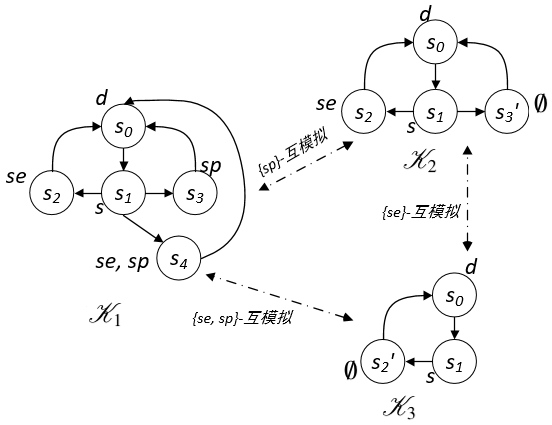
\includegraphics[width=8cm]{chapter03/NVBnewCar1.png}\\
		\caption{$\MPK$-结构之间的$V$-互模拟关系示意图}
		\label{Fig:chapter04:v1uv2}
	\end{figure*}
\end{example}



%$V$-互模拟给出了两个结构之间相互模仿的行为关系,下述命题给出了这种关系的一些关键性质。
下述命题给出了$V$-互模拟关系的一些关键性质。
\begin{proposition}\label{prop:bisimilar:V}
	给定集合$V_i\subseteq \Ha$、状态$s_i'$、路径$\pi_i'$和$\Ind$-结构${\cal K}_j=(\Hm_j,s_j)$,其中$i=1,2$,$j=1,2,3$。
	%令$i$是属于集合$\{1,2\}$的变量,$V_1$和$V_2$是$\Ha$的子集,$s_1'$和$s_2'$是两个状态,$\pi_1'$和$\pi_2'$是两条路径,${\cal K}_j=(\Hm_j,s_j)$$(j=1,2,3)$是$\Ind$-结构。
	如果${\cal K}_1 \lrto_{V_1} {\cal K}_2$且${\cal K}_2 \lrto_{V_2} {\cal K}_3$,则:
	\begin{itemize}
		\item[(i)] ${\cal K}_1\lrto_{V_1\cup V_2}{\cal K}_3$;
		\item[(ii)] 若 $V_1 \subseteq V_2$,则 ${\cal K}_1 \lrto_{V_2} {\cal K}_2$;
		\item[(iii)] $s_1'\lrto_{V_i}s_2'~(i=1,2)$ 蕴涵$s_1'\lrto_{V_1\cup V_2}s_2'$;
		\item[(iv)] $\pi_1'\lrto_{V_i}\pi_2'~(i=1,2)$ 蕴涵 $\pi_1'\lrto_{V_1\cup V_2}\pi_2'$;
		\item[(v)] 对$\Hm_1$上的每条路径 $\pi_{s_1}$,存在$\Hm_2$上的一条路径 $\pi_{s_2}$ 使得 $\pi_{s_1} \lrto_{V_1} \pi_{s_2}$,反之也成立。
	\end{itemize}
\end{proposition}
\begin{proof}
	%We prove the cases of $\MPK$-structures, and the cases of $\Ind$-structures are trivial.
	(i) 令 ${\cal M}_j=(S_j,R_j,L_j,[\_]_j,s_0^j)~(j=1,2,3)$,$\Hb$为$s_1$和$s_2$之间的$V_1$-互模拟关系,即 $s_1$ $\lrto_{V_1}$ $s_2$ 通过 $\Hb$形成$V_1$-互模拟关系,$s_2 \lrto_{V_2} s_3$通过$\Hb''$形成$V_2$-互模拟关系。 令 $\Hb' = \{(w_1,$ $w_3)\mid (w_1, w_2)\in \Hb$ 和 $(w_2, w_3)\in \Hb''\hbox{,其中}w_i\in S_i~(i=1,2,3)\}$。为了证明 ${\cal K}_1\lrto_{V_1\cup V_2}{\cal K}_3$,下证$\Hb'$ 是一个包含 $(s_1, s_3)$ 的 $V_1 \cup V_2$-互模拟关系。由于$(s_1,s_2)\in \Hb$ 和 $(s_2, s_3)\in \Hb''$,所以$(s_1, s_3) \in \Hb'$。
	% 		from the (a), (b) and (c) of the previous step (iii) of $X$-bisimulation (where $X$ is a set of atoms).
	对所有 $(w_1, w_3) \in \Hb'$,存在$w_2\in S_2$使得$(w_1, w_2)\in \Hb$和$(w_2, w_3)\in \Hb''$,且:
	\begin{itemize}
		\item[(a)] 存在一个 $w_2 \in S_2$使得 $(w_1,w_2)\in \Hb$ 且 $(w_2, w_3)\in \Hb''$。由 $w_1 \lrto_{V_1} w_2$可知;$L_1(w_1)$ $-V_1 = L_2(w_2) - V_1$;由$w_2 \lrto_{V_2} w_3$可知,$L_2(w_2) - V_2 = L_3(w_3) - V_2$。
		%			for all $q \notin V_1$, $q \in L_1(w_1)$ iff $q \in L_2(w_2)$ by $w_1 \lrto_{V_1} w_2$ and for all $q' \notin V_2$, $q'\in L_2(w_2)$ iff $q'\in L_3(w_3)$ by $w_2 \lrto_{V_2} w_3$. 
		所以,有 $L_1(w_1) - (V_1 \cup V_2) = L_3(w_3) - (V_1 \cup V_2)$。
		% for all $r\notin V_1 \cup V_2$, $r \in L_1(w_1)$ iff $r \in L_3(w_3)$.
		\item[(b)] $\forall u_1\in S_1$,若 $(w_1, u_1) \in R_1$,则 $\exists u_2\in S_2$ 使得$(w_2, u_2) \in R_2$ 和 $(u_1,u_2)\in \Hb$; 因而 $\exists u_3 \in S_3$ 使得$(w_3, u_3) \in R_3$ 且 $(u_2, u_3) \in \Hb''$,所以由 $\Hb'$的定义可知 $(u_1, u_3) \in \Hb'$。
		\item[(c)] $\forall u_3\in S_3$,若 $(w_3, u_3) \in R_3$,则 $\exists u_2\in S_2$ 使得 $(w_2, u_2) \in R_2$ 和 $(u_2, u_3) \in \Hb_2$;因此 $\exists u_1 \in S_1$ 使得  $(w_1, u_1) \in R_1$ 且 $(u_1, u_2) \in \Hb$,所以由 $\Hb'$的定义可知$(u_1, u_3) \in \Hb'$。
	\end{itemize}
	
	(ii) 假定 $\Hb_{V_1}$是$\Hm_1$ 和 $\Hm_2$之间的一个 $V_1$-互模拟关系,且 $(s_1, s_2)\in \Hb_{V_1}$。下证 $\Hb_{V_1}$ 也是$\Hm_1$ 和 $\Hm_2$之间的一个 $V_2$-互模拟关系。
	对任意 $(w_1, w_2) \in \Hb_{V_1}$,有:
	\begin{itemize}
		\item 因为$L_1(w_1) - V_1 = L_2(w_2) -V_1$ 和 $V_1 \subseteq V_2$,所以 $L_1(w_1) - V_2 = L_2(w_2) -V_2$;
		\item $\forall r_1 \in S_1$,若 $(w_1,r_1) \in R_1$,因为$\Hb_{V_1}$是$\Hm_1$ 和 $\Hm_2$之间的一个 $V_1$-互模拟关系, 则 $\exists r_2\in S_2$ 使得 $(w_2,r_2)\in R_2$ 且 $(r_1,r_2) \in \Hb_{V_1}$;
		\item $\forall r_2 \in S_2$,若 $(w_2,r_2) \in R_2$,因为$\Hb_{V_1}$是$\Hm_1$ 和 $\Hm_2$之间的一个 $V_1$-互模拟关系,则 $\exists r_1\in S_1$使得 $(w_1,r_1)\in R_1$ 且 $(r_1,r_2) \in \Hb_{V_1}$。
	\end{itemize}
	
	由于$V_i \subseteq (V_1 \cup V_2)$( $i = 1, 2$),则(iii)是 (ii)的一种特殊情况,因而(iv)从(iii)可以容易得到。
	
	(v) 因为$s_1 \lrto_{V_1} s_2$ (即:${\cal K}_1\lrto_{V_1}{\cal K}_2$),可以从$V$-互模拟的定义易证(v)。	
\end{proof}


在命题\ref{prop:bisimilar:V}中,性质(iii)-(v)的含义比较直观。性质(i)表示如果一个结构分别与另外的两个结构${\cal K}_1$和${\cal K}_3$具有$V_1$和$V_2$-互模拟关系,则${\cal K}_1$和${\cal K}_3$ 是 $V_1\cup V_2$-互模拟的(如图~\ref{Fig:chapter04:v1uv2}所示)。这一性质对遗忘性质的证明至关重要。性质(ii)表示若两个结构关于某一集合是互模拟的,则这两个结构关于该集合的超集是互模拟的。

从互模拟的定义来看,如果两个结构是$V$-互模拟的,那么对于与$V$中原子命题无关的公式$\varphi$来说,这两个结构同时满足或不满足$\varphi$。这一性质可以形式化地描述如下:

\begin{theorem}\label{thm:V-bisimulation:EQ}
	令$V\subseteq \Ha$是原子命题集,${\cal K}_i$ $(i=1,2)$是两个具有$V$-互模拟关系的$\Ind$-结构,即:${\cal K}_1 \lrto_V {\cal K}_2$。若$\Phi$是一个$\CTL$公式且$\IR(\Phi, V)$,则有${\cal K}_1\models \Phi$当且仅当${\cal K}_2\models \Phi$。
\end{theorem}
\begin{proof}
	下面通过归纳$\CTL$公式的结构证明这一结论。
	%这一结论可以从$\CTL$公式的结构归纳地来证明。此外,不失一般性地可以
	假设$\Var(\Phi) \cap V=\emptyset$,${\cal K}_1=(\Hm,s)$ 和 ${\cal K}_1=(\Hm',s')$。
	
	\textbf{基始.} $\Phi = p$ ($p\in \Ha -V$)。
	
	$(\Hm,s)\models \Phi$当且仅当$p\in L(s)$ \hfill (可满足关系的定义)\\
	$\LRto$ $p\in L'(s')$ \hfill ($s \lrto_V s'$)\\
	$\LRto$ $(\Hm',s') \models \Phi$。
	
	\textbf{归纳步.} (a) $\Phi = \neg \psi$。
	
	$(\Hm,s)\models \Phi$当且仅当$(\Hm,s) \not \models \psi$\\
	$\LRto$ $(\Hm',s')\not \models \psi$  \hfill (归纳假设)\\
	$\LRto$ $(\Hm',s') \models \Phi$。
	
	(b) $\Phi = \psi_1 \vee \psi_2$。
	
	$(\Hm,s)\models \Phi$\\
	$\LRto$ $(\Hm,s) \models \psi_1$或$(\Hm,s) \models \psi_2$\\
	$\LRto$ $(\Hm',s')  \models \psi_1$或$(\Hm',s') \models \psi_2$ \hfill (归纳假设)\\
	$\LRto$ $(\Hm',s') \models \Phi$。
	
	(c) $\Phi=\EXIST\NEXT\psi$。
	
	$(\Hm,s)\models \Phi$\\
	$\Rto$ 存在一条路径$\pi=(s,s_1,\dots)$使得$(\Hm,s_1)\models \psi$\\
	$\Rto$ 存在一条路径$\pi'=(s',s_1',\dots)$使得$\pi \lrto_V \pi'$且$(\Hm,s_1)\models \psi$\hfill ($s \lrto_V s'$,命题~\ref{prop:bisimilar:V})\\
	$\Rto$ $s_1 \lrto_V s_1'$且$(\Hm,s_1)\models \psi$ \hfill ($\pi \lrto_V \pi'$)\\
	$\Rto$ $(\Hm',s_1') \models \psi$   \hfill   (归纳假设)\\
	$\Rto$ $(\Hm',s')\models \Phi$。
	
	另一个方向可类似证明。
	
	(d) $\Phi = \EXIST \GLOBAL \psi$。
	
	$(\Hm,s)\models \Phi$\\
	$\Rto$ 存在一条路径$\pi=(s=s_0,s_1,\dots)$,使得对任意$i\ge 0$,都有$(\Hm,s_i)\models \psi$\\
	$\Rto$ 存在一条路径$\pi'=(s'=s_0',s_1',\dots)$,使得$\pi \lrto_V \pi'$,且对任意$i\ge 0$,都有$(\Hm,s_i)\models \psi$   \hfill ($s \lrto_V s'$,命题~\ref{prop:bisimilar:V})\\
	$\Rto$ 对于任意$i\ge 0$,都有$s_i \lrto_V s_i'$和$(\Hm,s_i)\models \psi$ \hfill ($\pi \lrto_V \pi'$)\\
	$\Rto$ 对于任意$i\ge 0$,都有$(\Hm,s_i') \models \psi$ \hfill (归纳假设)\\
	$\Rto$ $(\Hm',s')\models \Phi$。
	
	另一个方向可类似证明。
	
	(e) $\Phi = \EXIST (\psi_1 \UNTILL \psi_2)$。
	
	$(\Hm,s) \models \Phi$\\
	$\Rto$ 存在一条路径$\pi=(s=s_0,s_1,\dots)$和$i \ge 0$,使得$(\Hm,s_i) \models \psi_2$,且对所有的$0\leq j <i$都有$(\Hm,s_j)\models \psi_1$\\
	$\Rto$ 存在一条路径$\pi'=(s'=s_0',s_1',\dots)$,使得$\pi \lrto_V \pi'$和$(\Hm',s_i') \models \psi_2$,且对所有的$0\leq j <i$都有$(\Hm',s_j')\models \psi_1'$ \hfill ($s \lrto_V s'$,归纳假设,命题~\ref{prop:bisimilar:V})\\
	%$\Rto$ $(\Hm',s_i') \models \psi_2$,且对于所有的$0\leq j <i$,都有$(\Hm',s_j')\models \psi_1$  \hfill  \\
	$\Rto$ $(\Hm',s')\models \Phi$。
	
	另一个方向可类似证明。
\end{proof}

上述定理中,公式 $\Phi$不包含索引,否则, $\Ind$-结构中的索引函数可能会影响公式的可满足性。
例:令 $\phi=\EXIST_{\tuple{1}}\NEXT p$、
${\cal K}=(\Hm,s)$ 和 $\Hm=(S,R,L,[\_],s_0)$,其中 $S=\{s_0,s_1\}$, $L(s_0)=\emptyset$、 $L(s_1)=\{p\}$、
$R=\{(s_0,s_1),(s_0,s_0),(s_1,s_1), (s_1,s_0)\}$ 和 $[1]=\{(s_0,s_1), (s_1,s_1)\}$。显然,${\cal K}\models\phi$。
令 ${\cal K}'=(\Hm',s)$ 和 $\Hm'=(S,R,L,[\_]',s_0)$,其中 $[1]'=\{(s_0,s_0),(s_1,s_1)\}$。
显然,${\cal K}\lrto_{\{q\}}{\cal K}'$, $\IR(\phi,\{q\})$。但是,${\cal K}'\not\models\phi$。

\begin{example}
	令$\varphi_1 = d \wedge \EXIST\FUTURE se \wedge \ALL\GLOBAL(se \rto \ALL\NEXT d)$和$\varphi_2=d \wedge \ALL\NEXT se$是两个$\CTL$公式,且$\IR(\varphi_1,\{sp\})$ 和 $\IR(\varphi_2,\{sp\})$。因此,可以验证图\ref{Fig:chapter04:v1uv2}中的${\cal K}_1$和${\cal K}_2$都满足$\varphi_1$,但是都不满足$\varphi_2$。
\end{example}

\begin{definition}[互模拟等价,bisimilar equivalence]\label{def:bisimular:equivalene}
	给定原子命题集$V\subseteq {\cal A}$,公式$\varphi$和$\psi$。若对任意${\cal K}\models \varphi$,都存在一个${\cal K}'\models\psi$,使得${\cal K}\lrto_V{\cal K}'$;且对任意${\cal K}'\models\psi$,都存在一个${\cal K}\models \varphi$,使得${\cal K}\lrto_V{\cal K}'$,则称公式$\varphi$和 $\psi$是 {\em $V$-互模拟等价的(bisimilar equivalence)},记为 $\varphi\equiv_V\psi$。
\end{definition}

由定义\ref{def:VInd:bisimulation}和 \ref{def:bisimular:equivalene},和命题\ref{prop:bisimilar:V}可容易得出下列引理。
\begin{lemma}~\label{lem:eqR}
	对任意$V\subseteq\cal A$,  $\lrto_V$和 $\equiv_V$为等价关系。
\end{lemma}
\begin{proof}
	由命题\ref{prop:bisimilar:V}(i)可知 $\lrto_V$是传递的。显然也是自反和对称的。因此是等价关系。
	
	关系 $\equiv_V$显然是自反和对称的。
	假设$\varphi\equiv_V\psi$和 $\psi\equiv_V\xi$。则对任意 ${\cal K}\models\varphi$,由$\varphi\equiv_V\psi$可知,存在一个 ${\cal K}'\models\psi$使得${\cal K}'\lrto_V{\cal K}$;且由$\psi\equiv_V\xi$可知,存在一个 ${\cal K}''\models\xi$使得
	${\cal K}'\lrto_V{\cal K}''$。又因为$\lrto_V$是一个等价关系,因此,${\cal K}\lrto_V{\cal K}''$。类似地,对任意${\cal K}''\models\xi$,存在 ${\cal K}\models \varphi$ 使得${\cal K}''\lrto_V{\cal K}$。这表明$\equiv_V$是传递的。因此,$\equiv_V$是等价关系。
\end{proof} 


此外,由互模拟等价的定义和上述结论可得以下推论。%上面的定义和命题\ref{prop:bisimilar:V}蕴涵下面的推论。
% 	The below corollary follows from the above definition and Proposition~\ref{prop:bisimilar:V}.
\begin{corollary}~\label{cor:eqbi}
	令 $V$、$V_1$、$V_2$ 为$\cal A$的子集,$\varphi$和 $\psi$为公式。
	\begin{itemize}
		\item[(i)] 若 $\varphi\equiv\psi$,则 $\varphi\equiv_V\psi$。
		\item[(ii)] 若$\varphi$ 和 $\psi$不包括索引,且 $\varphi\equiv_\emptyset\psi$, 则 $\varphi\equiv\psi$。
		\item[(iii)] 若 $\varphi\equiv_{V_i}\psi~(i=1,2)$,则 $\varphi\equiv_{V_1\cup V_2}\psi$。
		\item[(iv)] 若 $\varphi\equiv_{V_1}\psi$ 和 $V_1\subseteq V_2$,则 $\varphi\equiv_{V_2}\psi$。
	\end{itemize}
\end{corollary}
\begin{proof}
	(i) 对任意$\varphi$(或 $\psi$)的模型 ${\cal K}$和$V \subseteq \Ha$,存在${\cal K} \lrto_V {\cal K}$。因此, $\varphi\equiv_V\psi$。
	
	(ii) 对任意$\varphi$的模型${\cal K}$,存在$\psi$的一个模型${\cal K}'$使得 ${\cal K} \lrto_{\emptyset} {\cal K}'$。显然 $\IR(\psi, \emptyset)$,由定理~\ref{thm:V-bisimulation:EQ}可知${\cal K} \models \psi$。类似地,对任意${\cal K}' \models \psi$,存在${\cal K} \models \varphi$使得 ${\cal K} \lrto_{\emptyset} {\cal K}'$,因此${\cal K}'\models \varphi$。
	
	(iii) 对任意${\cal K} \models \varphi$,存在${\cal K}' \models \psi$,使得 ${\cal K} \lrto_{V_i} {\cal K}'$ ($i=1,2$)。因此,由命题\ref{prop:bisimilar:V}(i)可知 ${\cal K} \lrto_{V_1\cup V_2} {\cal K}'$。类似地,对任意${\cal K}' \models \psi$,存在 ${\cal K} \models \varphi$,使得${\cal K} \lrto_{V_1\cup V_2} {\cal K}'$。因此,$\varphi\equiv_{V_1\cup V_2}\psi$。
	
	同理可证(iv)。
\end{proof}

请注意,在上述结论(ii)中  “$\varphi$和$\psi$不包含索引”是必要的。否则,令 $\varphi=\EXIST_{\tuple{1}}\NEXT p$ 和  
$\psi$ $=\EXIST_{\tuple{2}}\NEXT p$,可以证明,$\varphi\equiv_\emptyset \psi$,但是 $\varphi\not\equiv\psi$。
\begin{proposition}\label{prop:transform:V:EQ}
	令 $\varphi$为一个$\CTL$公式。则$\varphi\equiv_UT_\varphi$,其中 $T_\varphi=\CTLsnf(\varphi)$和
	$U=\Var(T_\varphi)-\Var(\varphi)$。
\end{proposition}
\begin{proof}
	令$T_0, T_1, \dots, T_n=T_{\varphi}$为转换过程产生的公式集合序列。$T_0=\{\ALL \GLOBAL(\start \rto p), \ALL \GLOBAL(p \rto \simp(\nnf(\varphi)))\}$,其中$p$是不出现在$\varphi$中的原子命题,且对任意$i$($0\leq i < n$),有$T_{i+1} = (T_i-\{\psi\}) \cup R_i$($Trans(\psi)$返回的结果为$R_i$)。此外,在这一过程中,所有公式都是否定范式形式。
	
	为了证明命题中的结论,只需证明,对任意$i$($0\leq i < n$),$T_i \equiv_{U} T_{i+1}$成立。由于$T_{i+1}$是由$T_i$通过表\ref{tab:trans}中的规则作用于$T_i$中的某一个公式得到,因此证明过程分为两个部分:(1)从$\varphi$到$T_0$部分;(2)从$T_0$到$T_{\varphi}$的部分。假设$\Hm_1=(S_1,R_1,L_1,[\_]_1,s_1)$和$\Hm_2=(S_2,R_2,L_2, [\_]_2, s_2)$。
	
	(1)下证$\varphi \equiv_{\{p\}} T_0$。
	
	$(\Rto)$ $\forall (\Hm_1, s_1) \in \Mod(\varphi)$,可以构造一个$\Ind$-Kripke结构$\Hm_2=(S_2,R_2,L_2,[\_],s_2)$,使得除了$L_2(s_2)=L_1(s_1) \cup \{p\}$(默认不出现在$\varphi$中的原子命题都不出现在状态的标签中),$\Hm_2$中的其它元素都与$\Hm_1$中的元素相同。显然,$(\Hm_2,s_2)\models T_0$且$(\Hm_1,s_1) \lrto_{\{p\}} (\Hm_2, s_2)$。
	
	$(\Lto)$ $\forall (\Hm_1,s_1) \in \Mod(T_0)$,由$\start$的语义可知$(\Hm_1,s_1) \models \varphi$。
	
	(2)下证对任意$i$($0\leq i < n$),有$T_i \equiv_{U} T_{i+1}$成立,其中$T_{i+1} = (T_i-\{\psi\}) \cup R_i$。这里,用$\psi \rto_t R_i$表示$R_i$是使用规则$t$在公式$\psi$上得到的结果,且$T_i=X\cup \{\psi\}$(显然,$T_{i+1}=X\cup R_i$,$X=T_i-\{\psi\}$)。下面证明规则$t\in \{$\textbf{Trans(1), Trans(4), Trans(6)}$\}$的情形,其它情形可以类似地证明。
	
	(a)$t=\textbf{Trans(1)}$。
	
	$(\Rto)$ $(\Hm_1,s_1)\in \Mod(T_i)$,即$(\Hm_1, s_1) \models X \wedge \ALL\GLOBAL(q \rto \EXIST \NEXT \varphi)$\\
	$\Rto$ $(\Hm_1,s_1) \models X$,且对任意路径$\pi=(s_{1,1},s_{1,2},\dots)$上的状态$s_{1,j}$ $(j\geq 1)$,有$(\Hm,s_{1,j}) \not \models \neg q$,或存在一个状态$s_{1,j+1}$使得$(s_{1,j},s_{1,j+1})
	\in R_1$且$(\Hm,s_{1,j+1}) \models \varphi$。
	
	由此构造一个初始$\Ind$-Kripke结构$\Hm_2$,使得$\Hm_2$与$\Hm_1$相同,除了:对使用规则 \textbf{Tra- ns(1)} 在公式$\ALL\GLOBAL(q \rto \EXIST \NEXT \varphi)$上而引入的新索引$ind$,有$[ind]_2=\bigcup_{s\in S} R_s \cup R_y$。其中:
	\begin{itemize}
		\item $R_{s_{1,j}}=\{(s_{1,j}, s_{1,j+1}), (s_{1,j+1}, s_{1,j+2}),\dots\}$ $(j\geq 1)$,其满足“若$(\Hm_1,s_{1,j}) \models q$,则$(\Hm_1,$ $s_{1,j+1})$ $\models \varphi$”且“对于任意$i\geq j$,若$(s_{1,i}, s') \in R_s\ (s \not= s_{1,j})$,则$s'=s_{1,i+1}$”;
		\item $R_y=\{(s_x,s_y)\mid s_x\in S$,若对任意$(s_1',s_2') \in \bigcup_{s\in S} R_s$, 有$s_1'\not= s_x$,则找一个状态$s_y\in S_2$,使得$(s_x,s_y)\in R_2\}$。
	\end{itemize}
	
	显然,$(\Hm_1,s_1) \lrto_{\emptyset} (\Hm_2,s_2)$\\
	$\Rto$ 对任意从$s_2$开始的路径$\pi=( s_2= s_{2,1} , s_{2,2}, \dots)$,如果$s_{2,j} \in \pi$,则$(\Hm_2,s_{2,j}) \models \neg q$或$(\Hm_2,$ $s_{2,j})\models \EXIST_{\tuple{ind}} \NEXT \varphi$\\
	$\Rto$ $(\Hm_2,s_2)\models \ALL\GLOBAL(q \rto \EXIST_{\tuple{ind}} \NEXT \varphi)$\\
	$\Rto$ $(\Hm_2,s_1) \models X \wedge \ALL\GLOBAL(q \rto \EXIST_{\tuple{ind}} \NEXT \varphi)$
	
	$(\Lto)$ $\forall (\Hm_1,s_1) \in \Mod(T_{i+1})$,即$(\Hm_1,s_1) \models X \wedge \ALL \GLOBAL(q \rto \EXIST_{\tuple{ind}} \NEXT \varphi )$\\
	$\Rto$ $(\Hm_1,s_1) \models X$且$(\Hm_1,s_1) \models \ALL \GLOBAL(q \rto \EXIST_{\tuple{ind}} \NEXT \varphi)$\\
	$\Rto$ 对任意以$s_1$为起点的路径上的任意状态$s_{1,j}$,$(\Hm_1,s_{1,j}) \models \neg q$或$(\Hm_1,s_{1,j}) \models \EXIST\NEXT\varphi$\\
	$\Rto$ $(\Hm_1,s_1) \models \ALL\GLOBAL(q \rto \EXIST \NEXT \varphi)$\\
	$\Rto$ $(\Hm_1,s_1) \models X \wedge \ALL\GLOBAL(q \rto \EXIST \NEXT \varphi)$。
	
	(b)$t=\textbf{Trans(4)}$。
	
	$(\Rto)$	$(\Hm_1,s_1) \in \Mod(T_i)$,即$(\Hm_1,s_1) \models X \wedge \ALL\GLOBAL (q \rto \varphi_1 \vee \varphi_2)$ \\
	$\Rto$ $(\Hm_1,s_1) \models X$,且$\forall s_1'\in S_1$,$(\Hm_1, s_1') \models q \rto \varphi_1 \vee \varphi_2$\\
	$\Rto$ $(\Hm_1,s_1')\models \neg q$或$(\Hm_1,s_1')\models \varphi_1 \vee \varphi_2$。
	
	如下构造初始$\Ind$-Kripke结构$\Hm_2=(S_2,R_2,L_2,[\_]_2,s_2)$:
	\begin{itemize}
		\item $S_2=S_1$,$R_2=R_1$,$[\_]_2$与$[\_]_1$相同,且$s_2=s_1$;
		\item $L_2$与$L_1$相同,除了:对任意$s_1'\in S_2$,若$(\Hm_1, s_1') \models \neg q$,则$L_2(s_1') = L_1(s_1')$,否则“若$(\Hm_1,s_1') \models \varphi_1$,则 $L_2(s_1')=L_1(s_1')$,否则$L_2(s_1')=L_1(s_1') \cup \{p\}$”。
	\end{itemize}
	显然,$(\Hm_2,s_1') \models (q\rto \varphi_1 \vee p) \wedge (p \rto \varphi_2)$且$(\Hm_1, s_1) \lrto_{\{p\}} (\Hm_2, s_2)$,所以,$(\Hm_2,s_2) \models T_{i+1}$。
	
	$(\Lto)$  $\forall (\Hm_1, s_1) \in \Mod(T_{i+1})$,即$(\Hm_1,s_1) \models X \wedge \ALL\GLOBAL (q\rto \varphi_1 \vee p) \wedge \ALL\GLOBAL(p \rto \varphi_2)$。 显然,$(\Hm_1, s_1) \models T_i$。
	
	(c)$t$=\textbf{Trans(6)}。
	
	这里证明$\EXIST_{\tuple{ind}} \NEXT$的情形,$\ALL \NEXT$的情形可以类似地证明。
	
	$(\Rto)$ $(\Hm_1,s_1) \in \Mod(T_i)$,即$(\Hm_1,s_1) \models X \wedge \ALL\GLOBAL(q \rto \EXIST_{\tuple{ind}}\NEXT \varphi)$\\
	$\Rto$ $(\Hm_1,s_1) \models X$,且对任意$s_1'\in S$,$(\Hm_1,s_1') \models q \rto \EXIST_{\tuple{ind}} \NEXT \varphi$\\
	$\Rto$ $(\Hm_1,s_1') \models \neg q$,或者存在一个状态$s'$,使得$(s_1', s') \in [ind]$且$(\Hm_1,s') \models \varphi$。
	
	如下构造初始$\Ind$-Kripke结构$\Hm_2=(S_2,R_2,L_2,[\_]_2,s_2)$:
	\begin{itemize}
		\item $S_2=S_1$,$R_2=R_1$,$[\_]_2$与$[\_]_1$一样且$s_2=s_1$;
		\item $L_2$与$L_1$相同,除了:对任意$s_1'\in S_2$,若$(\Hm_1, s_1') \models \neg q$,则$L_2(s_1') = L_1(s_1')$,否则“若$(\Hm_1,s_1') \models q$,则$L_2(s')$ $=L_1(s')\cup \{p\}$ $((s_1',s')\in R_2)$”。
	\end{itemize}
	显然,$(\Hm_2,s_2) \models \ALL\GLOBAL(q\rto \EXIST_{\tuple{ind}} \NEXT p) \wedge \ALL\GLOBAL(p \rto \varphi)$、$(\Hm_2,s_2) \models T_{i+1}$且$(\Hm_1, s_1) \lrto_{\{p\}} (\Hm_2, s_2)$ ($s_2=s_1$)。
	
	$(\Lto)$ $(\Hm_1, s_1) \in \Mod(T_{i+1})$,即$(\Hm_1,s_1) \models X \wedge \ALL\GLOBAL(q\rto \EXIST_{\tuple{ind}} \NEXT p) \wedge \ALL\GLOBAL(p \rto \varphi)$。显然,$(\Hm_1, s_1) \models T_i$。
\end{proof}
 
\begin{example}
	\label{examp:Tran}
	令 $\varphi=\ALL((p\wedge q) \UNTILL (f\vee m)) \wedge r$。 $T_{\varphi}$是下面子句构成的集合:
	\begin{align*}
		&  1: \start\rto z, &&  2: \top \rto \neg z \vee r, &&  3:\top \rto \neg x\vee f \vee m, &&
		4: \top \rto \neg z \vee x \vee y, \\
		&  5: \top \rto \neg y \vee p, &&  6: \top \rto \neg y \vee q, &&  7:  z \rto \ALL \FUTURE x, &&  8: y \rto \ALL \NEXT(x\vee y)
	\end{align*}
	其中 $x,y,z$ 为新引入的原子命题。
	%	$
	%	\begin{array}{llll}
	%		1. \start\rto z & 2. \top \rto \neg z \vee r \qquad & 3.\top \rto \neg x\vee f \vee m  & 4. \top \rto \neg z \vee x \vee y \\
	%		5.\top \rto \neg y \vee p &  6.\top \rto \neg y \vee q &
	%		7. z \rto \ALL \FUTURE x & 8. y \rto \ALL \NEXT(x\vee y),\\
	%	\end{array}
	%	$\\
	%	with the set $V'=\{x, y,z\}$ of new atoms introduced in this process, in which $w$ is a new atom related to $z \rto \ALL \FUTURE x$
	%~\footnote{Note that we always generate a new atom $w$ for each $Q$-sometime clause with $Q\in \{\EXIST, \ALL\}$ when this clause is produced during the transformation process.}. %~\cite{zhang2014resolution}.
	% Besides, the set of new atoms introduced in this process is $V'=\{x, y,z, w\}$ in which $w$ is a new atom related to $z \rto \ALL \FUTURE x$~\footnote{Note that we always generate a new atom for each $T$-sometime clause with $T\in \{\EXIST, \ALL\}$ when this clause is produced during the transform process.}. %~\cite{zhang2014resolution}.
\end{example}

\subsection{遗忘算子及其性质}
这部分给出$\CTL$遗忘的定义及其相关性质。

\begin{definition}[遗忘,forgetting]\label{def:V:forgetting}
	令$V$是$\Ha$的子集,$\Phi$是公式。如果公式$\psi$满足下面条件:
	%,记为$\CTLforget(\Phi, V)$:
	\begin{itemize}
		\item $\psi$与$V$中的原子命题无关(即:$\IR(\psi, V)$);
		\item $\Mod(\psi)=\{{\cal K}\mid {\cal K} \mbox{是一个初始$\Ind$-结构}, \exists {\cal K}'\in\Mod(\phi)\ \text{使得}\ {\cal K}'\lrto_V{\cal K}\}$。
	\end{itemize}
	%$V$中原子命题无关的公式(即:$\Var(\varphi) \cap V= \emptyset$) 
	那么,称$\psi$为从$\Phi$中遗忘$V$后得到的结果。
\end{definition}


从定义\ref{def:V:forgetting}可以看出,如果两个公式$\psi$和$\psi'$都是$\Phi$遗忘$V$中元素后得到的结果,则$\Mod(\psi)\equiv \Mod(\psi')$。从这个角度来看,$\Phi$遗忘$V$中元素后得到的所有结果是语义等价的。
将遗忘结果记为$\CTLforget(\phi,V)$,不做其它说明的情况下,这表示$\phi$遗忘$V$是$\CTL$可表示的。
此外,当$V$中只包含一个元素时,可以省略集合符号,即:$$\CTLforget(\Phi, \{p\}) \equiv \CTLforget(\Phi, p).$$ 

%值得指出的是,遗忘理论的定义与均匀插值的语义定义等价,也即是遗忘理论与均匀插值是一对对偶概念,这与其他逻辑(包括模态逻辑S4、S5和经典命题逻辑)中的说法一致~\cite{gfdf}。


遗忘的定义表明,如果公式$\psi$的任意一个模型${\cal K}$都能找到$\varphi$的一个模型${\cal K}'$使得${\cal K} \lrto_V {\cal K}'$,那么称$\psi$为$\varphi$遗忘$V$中原子命题后得到的结果。为刻画S5逻辑下遗忘的直观含义,Zhang等人提出了遗忘的特性——这些特性被称为\emph{遗忘理论公设}(forgetting postulates)~\cite{Yan:AIJ:2009}。
类似地,给定$\CTL$公式$\varphi$、$\varphi'=\CTLforget(\varphi, V)$、原子命题集$V\subseteq \Ha$和$\varphi'=\CTLforget(\varphi, V)$,$\CTL$下遗忘理论公设如下:
\begin{itemize}
	\item[(\W)] 削弱:$\varphi \models \varphi'$;
	\item[(\PP)] 正支持:对任意与$V$无关的公式$\eta$,若$\varphi \models \eta$则$\varphi' \models \eta$;
	\item[(\NgP)] 负支持:对任意与$V$无关的公式$\eta$,若$\varphi \not \models \eta$则$\varphi' \not \models \eta$;
	\item[(\textbf{IR})] 无关性: $\IR(\varphi', V)$。
\end{itemize}
其中(\W)和(\textbf{IR})表明,“遗忘”削弱了公式$\varphi$,且得到的结果与$V$无关;(\PP)和(\NgP)表明,对任意与$V$无关的公式$\eta$,$\varphi \models \eta$当且仅当$\varphi' \models \eta$。总而言之,遗忘结果能蕴涵所有与$V$无关且能被$\varphi$蕴涵的结果,不能蕴涵所有与$V$无关且不能被$\varphi$蕴涵的结果。
此外,这些公设不都是独立的(如:$\NP$由$\W$和$\PP$可以得出),但这里把它们都列出来以表达更加直观的含义。
从数据库和安全的层面讲,遗忘相当于从已有的关系表中构建一个视图,达到隐私保护的作用。
下面的定理表明上述公设对$\CTL$的遗忘是充分且必要的。
%下面的定理表明$\CTL$中的遗忘与上述公设也具有当且仅当的关系。

\begin{theorem}[表达性定理,Representation Theorem]\label{thm:close}
	%Let $\varphi$, $\varphi'$ and $\phi$ be \CTL\
	给定$\CTL$公式$\varphi$和$\varphi'$,$V \subseteq \Ha$为原子命题集。
	%Then t
	下面的陈述是等价的:
	\begin{itemize}
		\item[(i)] $\varphi' \equiv \CTLforget(\varphi, V)$,
		\item[(ii)] $\varphi'\equiv \{\phi \mid\varphi \models \phi \text{和} \IR(\phi, V)\}$,
		\item[(iii)] 若$\varphi$、$\varphi'$和$V$为(i)和(ii)中提到的符号,则公设(\W)、(\PP)、(\NgP)和(\textbf{IR})成立。
	\end{itemize}
\end{theorem}
\begin{proof}
	$(i) \LRto (ii)$. 通过证明如下等式证明该结论。%为了证明这个结论,只需证明如下等式成立:
	\[
	\Mod(\CTLforget(\varphi, V)) = \Mod(\{\phi \mid \varphi \models \phi, \IR(\phi, V)\}).\]
	$(\Rto)$ ${\cal K}'\models\CTLforget(\varphi, V)$\\
	$\Rto$  $\exists {\cal K}$使得${\cal K} \models \varphi$且${\cal K} \lrto_V {\cal K}'$ \hfill (定义~\ref{def:V:forgetting}) \\
	$\Rto$ $\forall \phi$,若$\varphi \models \phi$且$\IR(\phi, V)$,则${\cal K}' \models \phi$  \hfill (定理~\ref{thm:V-bisimulation:EQ})\\
	$\Rto$ ${\cal K}' \models \{\phi \mid \varphi \models \phi, \IR(\phi, V)\}$
	
	$(\Lto)$ 因为$\IR(\CTLforget(\varphi, V),V)$且$\varphi \models \CTLforget(\varphi, V)$,由定义~\ref{def:V:forgetting}可知$\{\phi \mid \varphi \models \phi, \IR(\phi, V)\} \models \CTLforget(\varphi, V)$。
	
	$(ii) \Rto (iii)$. 令$A = \{\phi \mid \varphi \models \phi, \IR(\phi, V)\}$。 
	首先,由于对任意$\phi'\in A$,都有$\varphi \models \phi'$,所以,$\varphi \models \varphi'$。
	其次,对任意公式$\phi$,若$\IR(\phi, V)$且$\varphi \models \phi$,则$\phi \in A$,因此,$\varphi' \models \phi$。
	第三, 对任意公式$\phi$,若$\IR(\phi, V)$且$\varphi \not \models \phi$,则$\phi \not \in A$。因此,$\varphi' \not \models \phi$。
	最后,因为对任意$\phi' \in A$,都有$\IR(\varphi',V)$ ,所以,$\IR(\phi',V)$。
	
	$(iii) \Rto (ii)$. 一方面,由(\PP) 和 (\NgP)可知,对任意公式$\phi'$且$\IR(\phi',V)$,$\varphi \models \phi'$当且仅当$\varphi' \models \phi'$。所以,对任意$\phi'\in \{\phi \mid \varphi \models \phi, \IR(\phi, V)\}$,都有$\varphi' \models \phi'$,所以,$\varphi' \models \{\phi \mid \varphi \models \phi, \IR(\phi, V)\}$。 
	另一方面,由 (\W) 和 (\textbf{IR})可知,$\{\phi \mid \varphi \models \phi, \IR(\phi, V)\} \models \varphi'$。因此,$\varphi'\equiv \{\phi \mid\varphi \models \phi, \IR(\phi, V)\}$。
\end{proof}

定理~\ref{thm:close}并不表明遗忘的结果一定存在。
%尽管上面的表达性定理描述了遗忘及其基本准则之间“当且仅当”的关系,值得注意的是上面的定义~\ref{def:V:forgetting}并不表示遗忘的结果一定存在。
事实上,存在一个$\CTL$公式和原子命题集,使得从该公式里遗忘该集合得到的结果不可用$\CTL$公式表达。
例:令$p$和 $x$为两个不同的原子命题,$\varphi(p,x)$\footnote{$\varphi(p,x)$ 表示具有原子命题集$\Var(\varphi)=\{p,x\}$的公式。}为下面公式合取~\cite{Maksimova:JANCL:1991}:
\begin{align*}
	&\ALL\GLOBAL(\neg x \wedge \neg \ALL \GLOBAL p \rto \neg \ALL \NEXT \neg x),
	\qquad \ALL\GLOBAL(\neg \ALL\NEXT \neg x \rto \ALL \NEXT x),\\
	& \ALL\GLOBAL(\ALL\NEXT x \rto \neg x \wedge \neg \ALL \GLOBAL p),
	\qquad \ALL\GLOBAL(x \rto \neg \ALL\GLOBAL p),
	\qquad \ALL\GLOBAL(\ALL \FUTURE \ALL \GLOBAL p).
\end{align*}
\citeauthor{Maksimova:JANCL:1991}证明了$\varphi(p,x)\land \varphi(p,y)\models x\lrto y$,且不存在$\CTL$公式 $\psi$使得 $\Var(\psi)=\{p\}$且$\varphi(p,x)$ $\models x\lrto \psi$,即$\CTL$不具有Beth性质。
这一结论蕴涵如下命题:
\begin{proposition}\label{pro:uniforget}
	$\CTLforget(x\land \varphi(p,x), \{x\})$ 在 $\CTL$中是不可表示的。
\end{proposition}
\begin{proof}
	令 $\psi(p)=\CTLforget(x\land \varphi(p,x), \{x\})$为一个$\CTL$公式。
	有 \\
	$\varphi(p,x)\land \varphi(p,y)\vdash x\lrto y$\\
	$\Rto$ $\varphi(p,x)\land x \vdash \varphi(p,y)\rto y$\\
	$\Rto$ $\varphi(p,x)\land x\vdash \psi(p)$ 和 $\psi(p)\vdash \varphi(p,y)\rto p(y)$\hfill (定理~\ref{thm:close})\\
	$\Rto$ $\varphi(p,x)\vdash x\rto\psi(p)$且$\varphi(p,y)\vdash \psi(p)\rto p(y)$,这表明$\varphi(p,x)\vdash \psi(p)\rto p(x)$\\
	$\Rto$ $\varphi(p,x)\vdash x\lrto \psi(p)$,这是一个矛盾。
\end{proof}




从命题公式$\varphi$中遗忘原子命题$p$为:$\Forget(\varphi,\{p\})\equiv\varphi[p/\bot] \vee \varphi[p/\top]$。
本文遗忘的定义对公式为命题逻辑公式时,与Lin等人于1994提出的命题逻辑遗忘一致,即:本文的$\CTL$遗忘扩展了命题逻辑遗忘。%下面命题展示了上述结论:

\begin{theorem}\label{thm:PL:CTL}
	给定一个命题公式$\varphi$和原子命题集$V\subseteq \Ha$,则下面逻辑等式成立。
	\[\CTLforget(\varphi, V) \equiv \Forget(\varphi,V).
	\]
\end{theorem}
\begin{proof}
%	为了证明上述结论成立,只需要证明$\Mod(\CTLforget(\varphi, V))= \Mod(\Forget(\varphi,V))$。	
	一方面,对于$\CTLforget(\varphi, V)$的任意一个模型$(\Hm, s)$,由遗忘的定义可知存在一个$\varphi$的模型$(\Hm',s')$使得$(\Hm, s)\lrto_V (\Hm',s')$。因而有$L(s)-V = L'(s')-V$(其中$L\in \Hm$,$L'\in \Hm'$),这表明$(\Hm,s)\models \Forget(\varphi,V)$。
	
	另一方面,对于$\Forget(\varphi,V)$的任意一个模型$(\Hm, s)$($\Hm=(S,R,L,[\_],s)$),存在$\varphi$的一个模型$(\Hm',s')$($\Hm'=(S',R',L',[\_]',s')$),使得$L(s)-V = L'(s')-V$。如下构建一个初始$\Ind$-结构$(\Hm_1,s_1)$,使得$\Hm_1=(S_1,R_1,L_1,[\_],s_1)$,其中:
	\begin{itemize}
		\item $S_1=(S-\{s\})\cup \{s_1\}$;
		\item $R_1$由将$R$出现的$s$替换为$s_1$得到;
		\item 对于$S_1$中任意一个状态$s^*$:
		\[L_1(s^*)=
		\left\{
		\begin{array}{ll}
			L'(s'), \quad \qquad \qquad \hbox{如果$s^*=s_1$;} \\
			L(s^*), \ \ \ \ \qquad \qquad \hbox{否则。}
		\end{array}
		\right.
		\]
	\end{itemize}
	
	显然,$(\Hm_1,s_1)$是$\varphi$的一个模型且$s_1 \lrto_V s$。因此,$(\Hm,s)$是$\CTLforget(\varphi,V)$的一个模型。
\end{proof}

遗忘的另一个重要性质与$V$-无关性密切相关。对于给定的公式$\psi=\varphi \wedge (q\lrto \alpha)$,如果$\IR(\varphi \wedge \alpha, \{q\})$,那么$\psi$遗忘$q$后得到的结果为$\varphi$。这一性质与后文将要介绍的$SNC$($WSC$)的计算密切相关。但是,由于其也是遗忘的性质,因而本文将其放在此处。
\begin{lemma}\label{lem:KF:eq}
	给定两个公式$\varphi$和$\alpha$,原子命题$q \not \in (\Var(\varphi) \cup \Var(\alpha))$,则:$$\CTLforget(\varphi \wedge (q \lrto \alpha), q)\equiv \varphi.$$
\end{lemma}
\begin{proof}
	$(\Rto)$ 令$\varphi'=\varphi \wedge (q \lrto \alpha)$。
	对于$\CTLforget(\varphi',q)$的任意模型$(\Hm,s)$,由遗忘的定义可知存在一个初始$\Ind$-结构$(\Hm',s')$,使得$(\Hm,s)\lrto_{\{q\}}(\Hm',s')$且$(\Hm',s')\models \varphi'$。
	显然,$(\Hm',s')\models \varphi$。
	此外,由于$\IR(\varphi, \{q\})$且$(\Hm,s)\lrto_{\{q\}}(\Hm',s')$,由定理~\ref{thm:V-bisimulation:EQ}可知$(\Hm,s)\models \varphi$。
	
		$(\Lto)$  令$\Hm=(S,R,L,[\_],s)$且$(\Hm,s)\in \Mod(\varphi)$。下面构造初始$\Ind$-结构$(\Hm',s)$,使得$\Hm'=(S,R,L',[\_],s)$,其中:
	\begin{align*}
		& L':S \rto 2^{\Ha}\ \mbox{且}\ \forall s^*\in S, \hbox{ 若}\ (\Hm, s^*) \not \models \alpha, \hbox{ 则 } L'(s^*) = L(s^*)-\{q\}\,  \hbox{ 否则 }\ L'(s^*) = L(s^*)\cup\{q\}, \\
		& \hbox{ 若}\ (\Hm, s) \models \alpha, \hbox{ 则 } L'(s) = L(s) \cup\{q\}, \ \hbox{ 否则}\ L'(s) = L(s)-\{q\}.
	\end{align*}
	
	显然,$(\Hm',s) \models \varphi$、$(\Hm',s)\models q \lrto \alpha$且$(\Hm',s) \lrto_{\{q\}} (\Hm,s)$。
	因此,$(\Hm',s) \models \varphi \wedge (q \lrto \alpha)$。所以,由$(\Hm',s) \lrto_{\{q\}} (\Hm,s)$可知,$(\Hm,s)\models \CTLforget(\varphi \wedge (q \lrto \alpha), q)$。
\end{proof}

%除了上述性质,遗忘还有其它一些一般性质。下面将详细介绍这些性质。

根据遗忘的定义可以看出,从一个公式里遗忘某个原子命题集中的元素是将该集合看作一个整体来遗忘的。下面的结论说明,遗忘原子命题集可分解为遗忘单个原子命题。
%遗忘可以将原子命题中的元素拿出来一个一个的遗忘,而不是作为一个整体。
\begin{proposition}[分解性,Decomposition]\label{disTF}
	对于给定的公式$\varphi$,原子命题集$V$,和原子命题$p$($p\not \in V$),下面的结论成立:
	\[
	\CTLforget(\varphi,\{p\}\cup V) \equiv \CTLforget(\CTLforget(\varphi,p),V).
	\]
\end{proposition}
\begin{proof}
%	要证明上述结论成立,只需证明等式左右两边的公式有相同的模型。	
	一方面,令$\Hm_1=(S_1,R_1,L_1,[\_],s_1)$是一个初始$\Ind$-Kripke结构,且$(\Hm_1,s_1)$是$\CTLforget(\varphi,$ $\{p\}\cup V)$的一个模型。由遗忘的定义可知,存在$\varphi$的一个模型$(
	\Hm,s)$($\Hm=(S,R,L,[\_],s)$)使得$(\Hm_1,s_1)\lrto_{\{p\}\cup V} (\Hm,s)$。
	如下构建一个初始$\Ind$-结构$(\Hm_2,s_2)$,使得$\Hm_2=(S_2,R_2,L_2,$ $[\_],s_2)$且:
	\begin{itemize}
		\item[(1)] 对于$s_2$情形:令$s_2$是满足下面条件的状态,
		\begin{itemize}
			\item $p \in L_2(s_2)$当且仅当$p\in L_1(s_1)$,
			\item 对任意$q \in V$,$q \in L_2(s_2)$当且仅当$q\in L(s)$,
			\item 对其它原子命题$q'$,$q' \in L_2(s_2)$,当且仅当$q'\in L_1(s_1)$,当且仅当$q'\in L(s)$。
		\end{itemize}
		
		\item[(2)] 其它情形:
		\begin{itemize}
			\item 对所有状态对$(w,w_1)$,若$w\in S$,$w_1\in S_1$且$w\lrto_{\{p\}\cup V} w_1$,如下构造$w_2\in S_2$:%对于所有的满足$w\in S$,$w_1\in S_1$且$w\lrto_{\{p\}\cup V} w_1$的状态对$(w,w_1)$,如下构造$w_2\in S_2$:
			\begin{itemize}
				\item $p \in L_2(w_2)$当且仅当$p\in L_1(w_1)$,
				\item 对任意$q \in V$,$q \in L_2(w_2)$当且仅当$q\in L(w)$,
				\item 对其它原子命题$q'$,$q' \in L_2(w_2)$,当且仅当$q'\in L_1(w_1)$,当且仅当$q'\in L(w)$。
			\end{itemize}
			\item 对于$(w_1',w_1)\in R_1$,若$w_2$由$w_1$构造而成,且$w_2'$由$w_1'$构造而成,则令$(w_2',w_2)\in R_2$。
		\end{itemize}
		\item[(3)] 删除$S_2$和$R_2$中重复的元素。
	\end{itemize}
	由此可知,$(\Hm, s) \lrto_{\{p\}} (\Hm_2, s_2)$且 $(\Hm_2, s_2) \lrto_V (\Hm_1, s_1)$。 所以,$(\Hm_2, s_2) \models \CTLforget(\varphi, p)$。 因此, $(\Hm_1,$ $s_1) \models \CTLforget(\CTLforget(\varphi, p), V)$。
	
	另一方面,若$(\Hm_1, s_1)$是$\CTLforget(\CTLforget(\varphi, p), V)$的一个模型,则存在一个初始-$\Ind$结构 $(\Hm_2, s_2)$,使得 $(\Hm_2, s_2) \models \CTLforget(\varphi, p)$且 $(\Hm_2, s_2) \lrto_V (\Hm_1, s_1)$;且存在 $(\Hm, s)$,使得$(\Hm,$ $s) \models \varphi$且 $(\Hm, s) \lrto_{\{p\}} (\Hm_2, s_2)$。因此,由命题~\ref{prop:bisimilar:V}(i)可知 $(\Hm, s) \lrto_{\{p\} \cup V} (\Hm_1, s_1)$,所以, $(\Hm_1,$ $s_1)$ $\models \CTLforget(\varphi, \{p\} \cup V)$。
\end{proof}

由上面的命题不难看出,从公式中遗忘原子命题集中的元素,可以将该集合拆成两个集合遗忘。
\begin{corollary}
	对于给定的公式$\varphi$,原子命题集$V_1$和$V_2$,有如下结论:
	\[
	\CTLforget(\varphi,V_1\cup V_2) \equiv \CTLforget(\CTLforget(\varphi,V_1),V_2).
	\]
\end{corollary}

类似于被遗忘的原子命题集能被拆成两个集合的遗忘,下面介绍在某些情况下,从带时序算子的公式中遗忘一些原子命题,可以将这些时序算子提到遗忘操作的前面。
\begin{proposition}
	令$V\subseteq \Ha$为原子命题集,$\phi$为$\CTL$公式,则下面等式成立:
	\begin{itemize}
		\item[(i)] $\CTLforget(\ALL\NEXT\phi,V) \equiv \ALL \NEXT\CTLforget(\phi,V)$;
		\item[(ii)] $\CTLforget(\EXIST\NEXT\phi,V) \equiv \EXIST \NEXT\CTLforget(\phi,V)$;
		\item[(iii)] $\CTLforget(\ALL\FUTURE\phi,V) \equiv \ALL\FUTURE\CTLforget(\phi,V)$;
		\item[(iv)] $\CTLforget(\EXIST\FUTURE\phi,V) \equiv \EXIST\FUTURE\CTLforget(\phi,V)$;
		\item[(v)] $\CTLforget(\ALL \GLOBAL\phi,V)\equiv \ALL \GLOBAL\CTLforget(\phi,V)$;
		\item[(vi)] $\CTLforget(\EXIST\GLOBAL\phi,V)\equiv\EXIST\GLOBAL \CTLforget(\phi,V)$。
	\end{itemize}
\end{proposition}
\begin{proof}
	(i) $(\Rto)$ $(\Hm,s)\models\CTLforget(\ALL\NEXT\phi,V)$\\
	$\Rto$ 存在$(\Hm,s)\lrto_V(\Hm',s')$且 $(\Hm',s')\models \ALL\NEXT\phi$\\
	$\Rto$  $(\Hm,s)\lrto_V(\Hm',s')$,且 对任意$(s',s'')\in R'$,有$(\Hm',s'')\models \phi$ \hfill ($R'\in\Hm'$)\\
	$\Rto$ 对任意$(s,s_1)\in R$,存在$(s',s'_1)\in R'$,使得$(\Hm,s_1)\lrto_V(\Hm',s'_1)$,且对任意$(s',s'')\in R'$,有
	$(\Hm',s'')\models \phi$\\
	$\Rto$ 对任意$(s,s_1)\in R$,有$(\Hm,s_1)\lrto_V(\Hm',s'_1)$且$(\Hm',s'_1)\models\phi$\\
	$\Rto$ 对任意$(s,s_1)\in R$, $(\Hm,s_1)\models\CTLforget(\phi,V)$\\
	$\Rto$ $(\Hm,s)\models\ALL\NEXT\CTLforget(\phi,V)$。
	
	$(\Lto)$ $(\Hm,s)\models\ALL\NEXT\CTLforget(\phi,V)$\\
	$\Rto$ 对任意$(s,s')\in R$, 有$(\Hm,s')\models\CTLforget(\phi,V)$ \hfill ($R\in \Hm)$\\
	$\Rto$ 对任意$(s,s')\in R$, 有$(\Hm,s')\lrto_V(\Hm',s'')$且$(\Hm',s'')\models\phi$\\
	$\Rto$ 对任意$i\ge 0$,有$(\Hm,s'_i)\lrto_V(\Hm'_i,s''_i)$且 $(\Hm'_i,s''_i)\models\phi$,
	其中 $\{s'_0,s'_1,\ldots\}=\{s'\mid (s,s')\in R\}$且 $\Hm'_i=(S'_i,R'_i,L'_i,[\_]'_i,s''_i)$ \hfill (当$i\neq j$时,假定$S'_i\cap S'_j=\emptyset$)\\
	$\Rto$ $(\Hm^*,s)\lrto_V(\Hm,s)$ 且 $(\Hm^*,s)\models\ALL\NEXT\phi$,其中
	$\Hm^*=(S^*,R^*,L^*,[\_], s)$且
	\begin{itemize}
		\item $S^*=\{s\}\cup\bigcup_{i\ge 0}S'_i$,
		\item $R^*=\{(s,s''_i)\mid i\ge 0\}\cup \bigcup_{i\ge 0} R'_i$,
		\item $L^*=\bigcup_{i\ge 0}L'_i$ 和 $L^*(s)=L(s)$,其中 $L\in\Hm$。
	\end{itemize}
	$\Rto$ $(\Hm,s)\models \CTLforget(\ALL\NEXT\phi,V)$。
	
	(ii) $(\Rto)$ $(\Hm,s)\models\CTLforget(\EXIST\NEXT\phi,V)$\\
	$\Rto$ 存在$(\Hm,s)\lrto_V(\Hm',s')$ 且 $(\Hm',s')\models \EXIST\NEXT\phi$\\
	$\Rto$ 存在$(\Hm,s)\lrto_V(\Hm',s')$,且对一些 $(s',s'')\in R'$,有$(\Hm',s'')\models \phi$ \hfill  ($R'\in\Hm'$)\\
	$\Rto$ 存在$(s,s_1)\in R$和$(s',s'_1)\in R'$,使得$(\Hm,s_1)\lrto_V(\Hm',s'_1)$,且存在$(s',s'')\in R'$,使得
	$(\Hm',$ $s'')\models \phi$ \hfill ($R\in \Hm$)\\
	$\Rto$ 存在$(s,s_1)\in R$和$(\Hm,s_1)\lrto_V(\Hm',s'_1)$,使得$(\Hm',s'_1)\models\phi$\\
	$\Rto$ 存在$(s,s_1)\in R$,使得$(\Hm,s_1)\models\CTLforget(\phi,V)$\\
	$\Rto$ $(\Hm,s)\models\EXIST\NEXT\CTLforget(\phi,V)$。
	
	$(\Lto)$ $(\Hm,s)\models\EXIST \NEXT\CTLforget(\phi,V)$\\
	$\Rto$ 对一些 $(s,s')\in R$, $(\Hm,s')\models\CTLforget(\phi,V)$  ($R\in \Hm)$\\
	$\Rto$ 对一些 $(s,s')\in R$,有$(\Hm,s')\lrto_V(\Hm',s'')$ 和 $(\Hm',s'')\models\phi$,其中 $\Hm'=(S',R',L',[\_]',s'')$ \\
	%		$\Rto$ For every $i\ge 0$, there is $(\Hm,s'_i)\lrto_V(\Hm'_i,s''_i)$ and $(\Hm'_i,s''_i)\models\phi$
	%		where $\{s'_0,s'_1,\ldots\}=\{s'\mid (s,s')\in R\}$ and $\Hm'_i=(S'_i,R'_i,L'_i,[\_]'_i,s''_i)$ (we assume $S'_i\cap S'_j=\emptyset$ when $i\neq j$)\\
	$\Rto$ $(\Hm^*,s)\lrto_V(\Hm,s)$ 和 $(\Hm^*,s)\models\EXIST\NEXT\phi$,其中
	$\Hm^*=(S^*,R^*,L^*,[\_], s)$,
	\begin{itemize}
		\item $S^*=S\cup S'$,
		\item $R^*=\{(s,s'')\}\cup R \cup R'$,
		\item $L^*= L \cup L'$ 且$L^*(s)=L(s)$,其中 $L\in\Hm$。
	\end{itemize}
	$\Rto$ $(\Hm,s)\models \CTLforget(\EXIST\NEXT\phi,V)$。
	
	
	
	
	(iii)和 (iv)可以分别类似 (i)和 (ii)来证明。
	
	(v) $(\Rto)$ $(\Hm,s) \models \CTLforget(\ALL \GLOBAL \phi, V)$\\
	$\Rto$ 存在$(\Hm',s') \models \ALL \GLOBAL \phi$且 $(\Hm,s) \lrto_V (\Hm',s')$\\
	$\Rto$ 对$\Hm$上的每一条路径$\pi=(s=s_1, s_2, \dots)$,存在$\Hm'$上的一条路径$\pi'=(s'=s_1, s_2', \dots)$,使得 $\pi \lrto_V \pi'$,反之也成立,且对任意$i\geq 1$,有$(\Hm', s_i') \models \varphi$\\ 
	%$\Rto$ For every $t' \in S'$, there is $(\Hm',t') \models \phi$ \quad ($S'\in \Hm'$) \\
	% $\Rto$ For every $t' \in S'$, there is $(\Hm',t') \models \CTLforget(\phi, V)$\\
	% $\Rto$ For every $t \in S$, there is $(\Hm,t) \models \CTLforget(\phi, V)$ \quad ($S\in \Hm$) \hfill ($\IR(\CTLforget(\phi, V), V)$)\\
	$\Rto$ 对$\pi$上的任意$s_i'$($i\geq 1$),有$(\Hm',s_i') \models \CTLforget(\phi, V)$\\
	$\Rto$ 对$\pi'$上的任意$s_i$($i\geq 1$),有$(\Hm,s_i) \models \CTLforget(\phi, V)$ \hfill ($\IR(\CTLforget(\phi, V), V)$)\\
	$\Rto$ 对任意$t \in S$,有$(\Hm,t) \models \CTLforget(\phi, V)$ \hfill ($S\in \Hm$)\\
	$\Rto$ $(\Hm,s) \models \ALL \GLOBAL \CTLforget(\phi, V)$。
	
	$(\Lto)$ $(\Hm, s) \models \ALL \GLOBAL \CTLforget(\phi, V)$\\
	$\Rto$ 对$\Hm$上的每一条路径 $\pi=(s=s_0, s_1, \dots)$,和任意$i \geq 0$,有$(\Hm,s_i) \models \CTLforget(\phi, V)$  \\ 
	$\Rto$ $\forall t \in S$, $(\Hm,t) \models \CTLforget(\phi, V)$ \hfill ($S \in \Hm$)\\
	$\Rto$ $\forall t \in S$,有$(\Hm,t) \lrto_V (\Hm',t')$且$(\Hm',t') \models \phi$\\
	$\Rto$ $\forall s_i \in S$ ($i \geq 0$),有$(\Hm,s_i) \lrto_V (\Hm_i',s_i')$且 $(\Hm_i',s_i') \models \phi$,其中$\Hm_i' = (S_i',R_i', L_i', [\_]_i',s_i')$\\
	$\Rto$ $(\Hm^*,s^*) \lrto_V (\Hm,s)$和$(\Hm^*,s^*) \models \ALL \GLOBAL \phi$,其中$\Hm^*= (S^*, R^*,L^*, [\_], s^*)$,
	\begin{itemize}
		\item $S^*= \bigcup S_i'$, %\{s_i \mid i \geq 0\}$,
		\item $s* = s_0'$,
		\item $R^* = \{(s_x', s_y') \mid (s_x, s_y) \in R,\ x, y \geq 0\} \cup \bigcup_{i \geq 0} R_i'$,其中 $R\in \Hm$,
		\item 对任意$t_i\in S_i'$,$L^*(t_i) = L_i'(t_i)$。
	\end{itemize}
	$\Rto$ $(\Hm,s) \models \CTLforget(\ALL \GLOBAL \phi, V)$。
	
	(vi) 可类似 (v)来证明。
\end{proof}


\begin{corollary}
	给定命题集合$V\subseteq \Ha$,命题公式$\varphi$和$\CTL$公式$\ALL\GLOBAL \psi$,则
	$$\CTLforget(\varphi \wedge \ALL\GLOBAL \psi)\equiv \CTLforget(\varphi \wedge \psi, V) \wedge \ALL\GLOBAL\CTLforget(\psi, V).$$
\end{corollary}
\begin{proof}
	 $(\Hm,s_0) \models \CTLforget(\varphi \wedge \ALL\GLOBAL \psi)$\\
	$\LRto$ 存在$(\Hm',s_0')  \lrto_V (\Hm,s_0)$,使得$(\Hm',s_0') \models \varphi \wedge \ALL\GLOBAL \psi$\\
	$\LRto$ 存在$(\Hm',s_0')  \lrto_V (\Hm,s_0)$,使得$(\Hm',s_0') \models \varphi \wedge \psi$且$(\Hm',s_0') \models \ALL\GLOBAL \psi$\\
	$\LRto$% 存在$(\Hm',s_0')  \lrto_V (\Hm,s_0)$,
	$(\Hm,s_0) \models \CTLforget(\varphi \wedge \psi,V)$且$(\Hm,s_0) \models \CTLforget(\ALL\GLOBAL \psi,V)$\\
%	$\LRto$ 存在$(\Hm',s_0')  \lrto_V (\Hm,s_0)$,使得$(\Hm',s_0') \models \CTLforget(\varphi \wedge \psi,V)$且$(\Hm',s_0') \models \ALL\GLOBAL\CTLforget( \psi,V)$\\
	$\LRto$ $(\Hm,s_0) \models \CTLforget(\varphi \wedge \psi,V)\wedge \ALL\GLOBAL\CTLforget( \psi,V)$。
\end{proof}
\section{$\mu$-演算遗忘理论}
\label{chapter03:sec:muforget}
$\mu$-演算是一种表达能力较强的逻辑语言,它能表达$\CTL$不能表达的一些性质,例如:Kripke结构中有一条路径,在这条路径上,基数位置的状态满足公式$\neg q \wedge \neg p$,但是偶数位置的状态满足$q \wedge p$。这一性质不能用$\CTL$公式来表达,但是可以用$\mu$-演算公式表达如下:
$$\varphi = \nu X.(p \wedge q) \wedge \EXIST \NEXT(\neg p \wedge \neg q) \wedge \EXIST \NEXT \EXIST \NEXT X.$$

这种情形在日常生活中是很常见的,如:偏序关系$(\mathbb{N}, \leq)$(自然数集上的小于等于关系)构成的Kripke结构,其基数节点为基数、偶数节点为偶数。
事实上,$\CTL$不能表达具有有规律的性质~\cite{DBLP:journals/iandc/Wolper83},其主要原因是
\begin{quote}
	\emph{对于给定的原子命题$p$,任意包含$n$个“$\NEXT$”时序算子的命题时序公式( proposinal temporal formula,PTL),对序列“$p^i(\neg p) p^w$”有相同的真值,其中$i > n$。%Given a proposition $p$, any proposinal temporal formula (PTL) $f(p)$ containing 
		%n ``next" ($\NEXT$) operators has the same truth value on all sequences of the form 
		%$p^i(\neg p) p^w$, $i > n$.
	}
\end{quote}

因而得出如下结论:
\begin{quote}
	\emph{对任意$m\geq 2$,性质“$p$在所有状态$s_i$上为真($i = k*m$,整数$k\geq 0$)”不能用PTL中的公式来表示。
		%For any given $m\geq 2$, the property ``$p$ is true in every 
		%state $s_i$, where $i = km$ (integer $k\geq 0$)" is not expressible in PTL.
	}
\end{quote}





本小节给出$\mu$-演算遗忘的定义,并说明本文所定义的$\mu$-演算遗忘与文章~\cite{d2006modal}中定义的均匀插值具有对偶关系。此时,本文给出的遗忘性质也是均匀插值所具有的性质,这为$\mu$-演算均匀插值的探索提供了另一种思路。此外,借助于均匀插值的计算方法,本文给出计算遗忘的方法。形成了遗忘和均匀插值之间相辅相成的作用。

本小节的组织结构如下。首先,给出变元-命题-互模拟的定义及证明变元-命题-互模拟对$\mu$-公式是不变的;根据变元-命题-互模拟定义$\mu$-演算遗忘;然后,探讨遗忘的性质,并给出其与均匀插值的关系;最后给出与遗忘相关问题的复杂性。

\subsection{变元-命题-互模拟}
与$\CTL$遗忘相似,这里先给出$V$-互模拟的定义。令$\Hm_i = (S_i, R_i, L_i, r_i)$,$i$为自然数集$\mathbb{N}$中的元素。
\begin{definition}[$V$-互模拟]\label{def:VB}
	给定原子命题集$V \subseteq \Ha$和两个Kripke结构$\Hm_1$和 $\Hm_2$。若$\Hb\subseteq S_1 \times S_2$满足下面几个条件:
	\begin{itemize}
		\item $r_1 \Hb r_2$,
		\item 对任意$s\in S_1$和 $t\in S_2$,若$s \Hb t$,则对任意$p \in \Ha- V$,有$p \in L_1(s)$当且仅当 $p \in L_2(t)$,
		\item 若$(s, s')\in R_1$和 $s \Hb t$,则存在一个 $t'$,使得$s' \Hb t'$和 $(t, t')\in R_2$,且
		\item 若 $s \Hb t$和$(t, t')\in R_2$,则存在一个$s'$,使得$(s, s')\in R_1$和 $t' \Hb s'$。
	\end{itemize}
则称$\Hb$是$\Hm_1$和 $\Hm_2$的$V$-互模拟关系。
\end{definition}

一方面,与$\CTL$下的$V$-互模拟不同的是:这里要求$r_1 \Hb r_2$(即:$(r_1,r_2)\in \Hb$)。
如果$\Hm_1$和 $\Hm_2$之间存在一个$V$-互模拟关系,那么${\cal B}$则称这两个Kripke结构$\Hm_1$和 $\Hm_2$及由这两个Kripke结构构成的结构$(\Hm_1,r_1)$和$(\Hm_2,r_2)$是$V$-互模拟的,分别记为$\Hm_1 \lrto_V \Hm_2$和$(\Hm_1,$ $r_1) \lrto_V (\Hm_2,r_2)$。
显然,Kripke结构之间的$V$-互模拟与结构之间的$V$-互模拟是等价的:$\Hm_1 \lrto_V \Hm_2$当且仅当$(\Hm_1,r_1) \lrto_V (\Hm_2,r_2)$。 因此,在下文中只讨论Kripke结构之间$V$-互模拟的性质,而结构之间的互模拟的性质与之相同。不难看出初始结构之间的$V$-互模拟是结构之间的$V$-互模拟的一个特例。


另一方面,$V$-互模拟与${\cal L}$-互模拟
%\footnote{${\cal L}$-互模拟是一种将定义\ref{def:VB}中的$V$替换为${\cal L}$的二元关系。}
~\cite{d1996uniform}类似,不同的是$V$-互模拟只考虑原子命题,且当${\cal L}$为原子命题集时是${\cal L}$-互模拟补命题(这里默认除了原子命题之外的符号都是相同的,因此只考虑原子命题)。
此外,已有结果表明${\cal L}$-句子(符号只出现在${\cal L}$中的$\mu$-句子)关于${\cal L}$-互模拟是{\em 不变的},即若$\Hm$和 $\Hm'$是${\cal L}$-互模拟的,则对于${\cal L}$-句子$\varphi$有$\Hm \models \varphi$当且仅当$\Hm' \models \varphi$~\cite{d1996uniform,bradfield2018mu}。
因此,若$\IR(\varphi, V)$且$\Hm \lrto_V \Hm'$,则$\Hm \models \varphi$当且仅当$\Hm' \models \varphi$。
本文称这一性质为$V$-不变性。
%值得注意的是这里的结构之间的$V$-互模拟是$\CTL$
%In this case, $\Hm_1$ and $\Hm_2$ are bisimilar on $V$.
\begin{example}\label{exmp:c06:bisim}
	 令$\varphi= \nu X.( ch \wedge j \wedge  \EXIST \NEXT \EXIST \NEXT X)$,易证下面两个赋值$(\Hm,v)$和$(\Hm',v')$(图~\ref{chapter06:fig:bisim}中的两个Kripke结构)
	 是$\varphi$的模型,其中
	\begin{itemize}
		\item $\Hm=(S,r,R,L)$,其中$S=\{s_0,s_1,s_2\}$,$r=s_0$,$L(s_0)=\{ch, j\}$,$L(s_1)=\{ch\}$,$L(s_2)=\emptyset$,$R=\{(s_0,s_1), (s_1,s_0), (s_0,s_2), (s_2,s_0)\}$,$v(X)=\{s_0\}$,
		\item  $\Hm'=(S',r',R',L')$,其中$S'=\{t_0,t_1\}, r'=t_0$,$L'(t_0)=\{j\}$,$L'(t_1)=\emptyset$,$R'=\{(t_0,t_1),$ $(t_1,$ $t_0)\}$且
		$v'(X)=\{t_0\}$。
	\end{itemize} 
	
		\begin{figure}[h]%
		\centering
		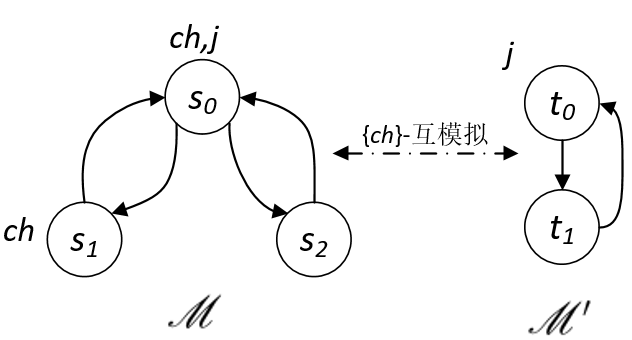
\includegraphics[width=5cm]{chapter06/chvB3.png}
		\caption{两个 $\{ch\}$-互模拟的Kripke结构示意图}\label{chapter06:fig:bisim}
		
		% $s_0$ is labeled by $\{ch, j\}$, $t_0$ is labeled by $\{j\}$, and $s_1$, $s_2$, and $t_1$ are labeled by $\emptyset$.}\label{fig:bisim}
	\end{figure}
	
	由于$\Hm$和 $\Hm'$之间存在一个$\{ch\}$-互模拟关系$\Hb=\{(s_0, t_0), (s_1, t_1), (s_2, t_1)\}$,所以,$\Hm \lrto_{\{ch\}}$ $\Hm'$。
\end{example}
%\begin{example}
%	\label{exmp:c06:bisim}
%	如图\ref{chapter06:fig:bisim}中的两个Kripke结构$\Hm=(S,R,L,r)$和 $\Hm'=(S',R',L',r')$,其中:
%	\begin{itemize}
%		\item $S=\{s_0,s_1,s_2\}$,$S'=\{t_0,t_1\}$,$r=s_0$,$r'=t_0$;
%		\item $R=\{(s_0,s_1),(s_1,s_0),(s_0,s_2),(s_2,s_0)\}$,$R'=\{t_0,t_1\}$;
%		\item $L(s_0)=\{ch,j\}$,$L(s_1)=\{ch\}$,$L(s_2)=\emptyset$,$L'(t_0)=\{j\}$,$L'(t_1)=\emptyset$。
%	\end{itemize}
%	由于$\Hm$和 $\Hm'$之间存在一个二元$\{ch\}$-互模拟$\Hb=\{(s_0, t_0), (s_1, t_1), (s_2, t_1)\}$,所以 $\Hm \lrto_{\{ch\}} \Hm'$。%,所以$\Hm\lrto \Hm'$。
%	
%	
%	
%	% 	\begin{center}\label{fig:bisim}
%	% 		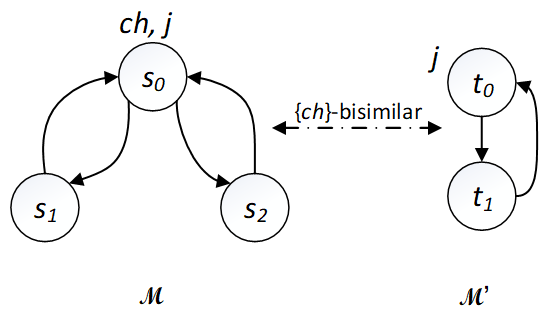
\includegraphics[width=5cm,height=3cm]{chBisimilar.png}\\
%	% 		%\vspace{2mm}
%	% 		\parbox[c]{7cm}{\textbf{Fig.1~}  Two $\{ch\}$-bisimilar Kripke structures}%\vspace*{.2mm}
%	% 	\end{center}
%	
%	\begin{figure}[h]%
%		\centering
%		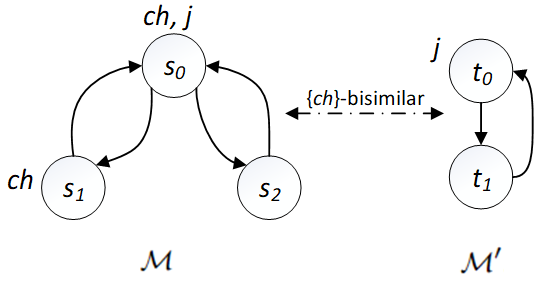
\includegraphics[width=4.5cm,height=2.5cm]{chapter06/chvB1.png}
%		\caption{两个 $\{ch\}$-互模拟的Kripke结构示意图}\label{chapter06:fig:bisim}
%		
%		% $s_0$ is labeled by $\{ch, j\}$, $t_0$ is labeled by $\{j\}$, and $s_1$, $s_2$, and $t_1$ are labeled by $\emptyset$.}\label{fig:bisim}
%	\end{figure}
%	
%\end{example}

$\mu$-句子互模拟是不变的,$\mu$-公式则不是~\cite{janin1996expressive}。这里定义一种对$\mu$-公式是不变的互模拟。

\begin{definition}[变元-命题-互模拟]
	给定$V \subseteq \Ha$、${\cal V}_1 \subseteq {\cal V}$、$\Hm_i = (S_i, r_i, R_i, L_i)$为Kripke结构、 $s_i\in S_i$且
	$v_i: {\cal V} \rto 2^{S_i}$,其中$i\in\{1,2\}$。若关系$\Hb\subseteq S_1 \times S_2$满足:
	\begin{itemize}
		\item $(s_1,s_2)\in\Hb$,
		\item $\Hb$是$\Hm_1$ 和$\Hm_2$之间的$V$-互模拟,且
		\item 对任意$(t_1,t_2)\in \Hb$和$X  \in {\cal V}-{\cal V}_1$,$t_2\in v_2(X)$当且仅当$t_1 \in v_1(X)$。
	\end{itemize}	
则称$\Hb$是$(\Hm_1,s_1, v_1)$ 和$(\Hm_2,s_2, v_2)$之间的一个{\em $\tuple{{\cal V}_1, V}$-互模拟}。
\end{definition}
%
%\begin{definition}[Var-$V$-互模拟]
%	\label{def:varVb}
%	给定原子命题集合$V$、赋值$(\Hm, v)$和$(\Hm',v')$。$(\Hm, v)$和$(\Hm',v')$之间的一个Var-$V$-互模拟关系$\Hb$是$\Hm$和$\Hm'$之间一个$V$-互模拟关系,且满足:
%	若 $(s,s') \in {\cal B}$,则对任意$X\in {\cal V}$, $s\in v(X)$ 当且仅当 $s'\in v'(X)$。
%\end{definition}

若$(\Hm,s, v)$和$(\Hm',s',v')$之间存在一个$\tuple{{\cal V}_1, V}$-互模拟关系$\Hb$,则称$(\Hm,s, v)$和$(\Hm',s',$ $v')$是$\tuple{{\cal V}_1, V}$-互模拟的,记为$(\Hm,s, v)\lrto_\tuple{{\cal V}_1, V} (\Hm',s',v')$。
若$(\Hm,s, v)$和$(\Hm',s',v')$之间存在一个$\tuple{\emptyset, V_1}$-互模拟关系,则称$(\Hm,s, v)$和$(\Hm',s',v')$是{\em Var-$V_1$-互模拟的},记为$(\Hm, s,v) $ $\lrto_{V_1} (\Hm',s',v')$;称$\tuple{\emptyset, V_1}$-互模拟为Var-$V_1$-互模拟。此外,若$s=r$ 且$s'=r'$,则$(\Hm, s,v) $ $\lrto_{\tuple{{\cal V}_1, V}} (\Hm',s',v')$简写为$(\Hm, v) \lrto_{\tuple{{\cal V}_1, V}} (\Hm',v')$。

显然,若$({\cal M},s,v)\lrto_V({\cal M}',s',v')$,则${\cal M}\lrto_V{\cal M}'$。
$\Hm\lrto_V\Hm'$,但$(\Hm,v)\not\lrto_V(\Hm',v')$ 有时是成立的。例:例~\ref{exmp:c06:bisim}中的两个Kripke结构$\Hm$ 和 $\Hm'$ 是$\emptyset$-互模拟的。然而,由于$r_1\in v(X)$和$(r_1,r_2')\in\Hb$,但是$r_2'\not\in v'(X)$,所以$(\Hm,v)\not\lrto_\emptyset (\Hm',v')$。
对$S_1\subseteq S$和二元关系$\Hb\subseteq S \times S'$,记$\Hb(S_1) =\{s' \mid (s, s')\in \Hb,\ s \in S_1\}$。

再者,对任意$X\in {\cal V}$,令$v(X)=S$且$v'(X)=S'$,Kripke结构${\cal M}$和${\cal M}'$之间的任意$V$-互模拟可以容易地扩展为$({\cal M},r,v)$和$({\cal M}',r',v')$之间的Var-$V$-互模拟,其中$S$和$S'$分别为$\Hm$和$\Hm'$中的状态集合。

\begin{example}[例~\ref{exmp:c06:bisim}的延续]
	令 $\Hm$和 $\Hm'$为图~\ref{chapter06:fig:bisim}中的Kripke结构,$v: {\cal V} \rto 2^S$和$v': {\cal V} \rto 2^{S'}$为将${\cal V}$中的变元分别赋值到$\Hm$和$\Hm'$的状态集上的赋值函数。可以检查下面的结论成立:
	\begin{itemize}
		\item 若对任意$X\in\cal V$,$v(X)= \{s_0, s_1, s_2\}$ 且$v'(X)=\{t_0, t_1\}$,则$({\cal M},v)\lrto_{\{ch\}} ({\cal M}',v')$;
		
		\item 若对任意$X\in{\cal V}-\{X_1\}$,$v(X_1)= \{s_0\}$、$v'(X_1)=\{t_1\}$、$v(X)= \{s_0, s_1, s_2\}$且$v'(X)=\{t_0, t_1\}$,则$({\cal M},v)\not\lrto_{\{ch\}} ({\cal M}',v')$;这是因为$(s_0,t_0)\in {\cal B}$且 $s_0\in v(X_1)$,但是$t_0\notin v'(X_1)$。
	\end{itemize}
\end{example}



可以证明$\lrto_V$有如下性质。

\begin{proposition} \label{pro:EqUnion}
	令${\cal V}_1, {\cal V}_2\subseteq {\cal V}$、$V, V_1 \subseteq \Ha$且$\Hm_i$为Kripke结构($i=1,2,3$),若$v_i: {\cal V}\rto 2^{S_i}$,则:
	\begin{enumerate} [(i)]
		\item $\lrto_{\tuple{{\cal V}_1,V}}$为赋值间的等价关系;
		\item 若$(\Hm_1, s_1,v_1) \lrto_{\tuple{{\cal V}_1,V}} (\Hm_2,s_2,v_2)$、${\cal V}_1 \subseteq {\cal V}_2$且$V \subseteq V_1$,\\
		则 $(\Hm_1, s_1, v_1) \lrto_{\tuple{{\cal V}_2,V_1}} (\Hm_2, s_2, v_2)$;
		\item 若$(\Hm_1, s_1, v_1) \lrto_{\tuple{{\cal V}_1,V}} (\Hm_2,s_2, v_2)$且$(\Hm_2,s_2, v_2) \lrto_{\tuple{{\cal V}_2,V_1}} (\Hm_3,s_3, v_3)$,\\
		则 $(\Hm_1,s_1,v_1) \lrto_{\tuple{{\cal V}_1 \cup {\cal V}_2, V \cup V_1}} (\Hm_3,s_3,v_3)$。
	\end{enumerate}
%	令$V, V_1 \subseteq \Ha$为原子命题集,$(\Hm_1,v_1)$、 $(\Hm_2,v_2)$和$(\Hm_3,v_3)$为赋值,则:
%	\begin{itemize} 
%		\item[(i)] $\lrto_V$是 赋值之间的等价关系;
%		\item[(ii)] 若$(\Hm_1, v_1) \lrto_V (\Hm_2,v_2)$ 和$V \subseteq V_1$,则$(\Hm_1, v_1) \lrto_{V_1} (\Hm_2,v_2)$;
%		\item[(iii)] 若 $(\Hm_1, v_1)  \lrto_V (\Hm_2,v_2)$且 $(\Hm_2,v_2) \lrto_{V_1} (\Hm_3,v_3)$,则 $(\Hm_1, v_1) \lrto_{V \cup V_1} (\Hm_3,v_3)$。
%	\end{itemize}
%	
\end{proposition}
\begin{proof}
%	Let $\Hm_i = (S_i, r_i, R_i, L_i)$ be Kripke structures, and $v_i: {\cal V} \rto 2^{S_i}$ be valuations of the variables in ${\cal V}$ to the states of $\Hm_i$ ($i=1,2,3$).
	
	(i) 这里从自反性、对称性和传递性来证明该关系是一个等价关系。
	
	(a) $\lrto_V$是自反的。显然,对任意的赋值$(\Hm,s,v)$都有$(\Hm,s,v)\lrto_{\tuple{{\cal V}_1,V}} (\Hm,s,v)$。
	
	(b) 对称性: % $\lrto_V$ is symmetric. 
	下证对任意$(\Hm_1,s_1, v_1)$和$(\Hm_2,s_2,v_2)$,若$(\Hm_1,s_1, v_1) \lrto_{\tuple{{\cal V}_1,V}} (\Hm_2,s_2,v_2)$,则$(\Hm_2,s_2, v_2) \lrto_{\tuple{{\cal V}_1,V}} (\Hm_1,s_1, v_1)$。
	假定$(\Hm_1, s_1,v_1)$ 和$(\Hm_2,s_2,v_2)$ 有${\tuple{{\cal V}_1,V}}$-互模拟关系$\Hb$,如下构造关系$\Hb_1$:$\Hb_1=\{(s,t) \mid (t, s)\in \Hb\hbox{,其中 } t\in S_1 \hbox{和} s\in S_2\}$。下证$\Hb_1$是$\Hm_2$$\Hm_1$之间的$V$-互模拟关系。
	\begin{itemize}
		\item 因为 $(r_1,r_2) \in \Hb$,所以,$(r_2,r_1) \in \Hb_1$;
		\item 对任意$s\in S_2$ 和$t\in S_1$,若$(s,t) \in \Hb_1$,则$(t,s) \in \Hb$。因此,对任意$p \in \Ha - V$,$p \in L_1(t)$当且仅当$p \in L_2(s)$;
		\item 因为$\Hb$是$\Hm_1$和 $\Hm_2$之间的$V$-互模拟关系,所以$V$-互模拟的第三和第四个点很容易能够证明。
	\end{itemize}
	此外,若$(t,s) \in \Hb$,则对任意$X\in {\cal V} -{\cal V}_1$,$s \in v_1(X)$ 当且仅当$t \in v_2(X)$。因此,若$(s,t) \in \Hb_1$, 则对任意$X\in {\cal V} -{\cal V}_1$,$t \in v_2(X)$ 当且仅当$s\in v_1(X)$。所以, $(\Hm_2,s_2, v_2) \lrto_{\tuple{{\cal V}_1,V}} (\Hm_1,s_1, v_1)$。

	(c) 传递性:%$\lrto_V$ is transitive. 
	下证若$(\Hm_1,s_1,v_1) \lrto_{\tuple{{\cal V}_1,V}} (\Hm_2,s_2,v_2)$和$(\Hm_2,s_2,v_2) \lrto_{\tuple{{\cal V}_1,V}} (\Hm_3,s_3,v_3)$, 则$(\Hm_1,s_1,v_1) \lrto_{\tuple{{\cal V}_1,V}} (\Hm_3,s_3,v_3)$。$(\Hm_1,s_1,v_1)$和$(\Hm_2,s_2,v_2)$有${\tuple{{\cal V}_1,V}}$-互模拟关系$\Hb_1$,$(\Hm_2$ $,s_2,v_2)$ $(\Hm_3,s_3,v_3)$有${\tuple{{\cal V}_1,V}}$-互模拟关系$\Hb_2$,如下构造$\Hb$:$\Hb=\{(s, z) \mid (s,t) \in \Hb_1\ \mbox{和}\ (t, z)$ $\in \Hb_2 \hbox{,其中} s\in S_1,  t\in S_2, \hbox{和} z \in S_3\}$。
	可以类似(b)证明$\Hb$是$\Hm_1$和$\Hm_3$之间的$V$-互模拟关系。因此,$\Hm_1 \lrto_{\tuple{{\cal V}_1,V}} \Hm_3$。
	
	此外,若$(s,t) \in \Hb$,则存在$t \in S_2$使得$(s,t)\in \Hb_1$和$(t,z)\in \Hb_2$。
	因此,对任意$X\in {\cal V}-{\cal V}_1$,$s \in v_1(X)$ 当且仅当$t \in v_2(X)$当且仅当$z\in V_3(X)$。所以,$(\Hm_2, v_2) \lrto_V (\Hm_1, v_1)$。
	

	
 (ii) 假定$\Hb_{V}$是$(\Hm_1,s_1,v_1)$和$(\Hm_2,s_2,v_2)$之间的${\tuple{{\cal V}_1,V}}$-互模拟关系。下证$\Hb_{V}$也是$(\Hm_1,$ $s_1,v_1)$和 $(\Hm_2,s_2,v_2)$之间的${\tuple{{\cal V}_2,V_1}}$-互模拟关系。
		显然:
		\begin{itemize}
			\item $(r_1, r_2) \in \Hb_{V}$;
			\item 对任意$w_1\in S_1$和$w_2\in S_2$,若$(w_1, w_2) \in \Hb_{V}$,则对任意$p \in \Ha - V_1$,
			$p\in L_1(w_1)$当且仅$p\in L_2(w_2)$(因为$V \subseteq V_1$且对任意$p \in \Ha - V$,$p\in L_1(w_1)$当且仅当$p\in L_2(w_2)$);
			%$L_1(w_1) - V_1 = L_2(w_2) -V_1$ since $L_1(w_1) - V = L_2(w_2) -V$ and $V \subseteq V_1$,
			\item 因为$\Hb_{V}$ 是$\Hm_1$和$\Hm_2$之间的$V$-互模拟,所以$V$-互模拟的第三和第四个点很容易能够证明。
			%$\forall r_1 \in S_1$, 
%			若$(w_1,r_1) \in R_1$且$(w_1, w_2)\in \Hb_V$,则$\exists r_2\in S_2$,使得$(w_2,r_2)\in R_2$和$(r_1,r_2) \in \Hb_{V}$(因为$\Hb_{V}$ 是$\Hm_1$ and $\Hm_2$之间的$V$-互模拟);
%			\item %$\forall r_2 \in S_2$, 
%			if $(w_2,r_2) \in R_2$ and $(w_1, w_2)\in \Hb_V$, then $\exists r_1\in S_1$ s.t. $(w_1,r_1)\in R_1$ and $(r_1,r_2) \in \Hb_{V}$ since $\Hb_{V}$ is a $V$-bisimulation between $\Hm_1$ and $\Hm_2$。
	\end{itemize}
	因此,$\Hb_{V}$ 是$\Hm_1$ 和$\Hm_2$之间的$V_1$-互模拟。
	
	此外,若$(s,t) \in \Hb_V$,则对任意$X\in {\cal V}-{\cal V}_2$,$s \in v_1(X)$ 当且仅当$t \in v_2(X)$。因此,$(\Hm_1, s_1, v_1) \lrto_{\tuple{{\cal V}_2,V_1}} (\Hm_2,s_2,v_2)$。
	
	
	(iii) 由(ii)可知,若$(\Hm_1,s_1,v_1) \lrto_{\tuple{{\cal V}_1,V}} (\Hm_2,s_2,v_2)$,则$(\Hm_1,s_1,v_1) \lrto_{\tuple{{\cal V}_1 \cup {\cal V}_2,V \cup V_1}} (\Hm_2,s_2,$ $v_2)$。因此,由(i)可知$(\Hm_1,s_1,v_1) \lrto_{\tuple{{\cal V}_1 \cup {\cal V}_2,V \cup V_1}} (\Hm_3,s_3,v_3)$。	
%	(i) 这里从自反性、对称性和传递性来证明该关系是一个等价关系。
%	
%	(1) $\lrto_V$是自反的。显然,对任意的赋值$(\Hm,v)$都有$(\Hm,v)\lrto_V (\Hm,v)$。
%	
%	(2) $\lrto_V$是对称的。 下证对任意$(\Hm_1, v_1)$ 和$(\Hm_2,v_2)$,若$(\Hm_1,v_1) \lrto_V (\Hm_2,v_2)$,则$(\Hm_2,$ $ v_2) \lrto_V (\Hm_1, v_1)$。
%	假设 $(\Hm_1, v_1)$和$(\Hm_2,v_2)$之间的Var-$V$-互模拟关系$\Hb$,构造如下二元关系:$\Hb_1=\{(s,t) \mid (t, s)\in \Hb\}$。现在从下面几点证明 $\Hb_1$ 是$\Hm_2$和 $\Hm_1$之间的一个$V$-互模拟关系:
%	\begin{itemize}
%		\item 由于$r_1 \Hb r_2$,所以$r_2 \Hb_1 r_1$,
%		\item 对任意$s\in S_1$和 $t\in S_2$,若 $t \Hb_1 s$,则 $s\Hb t$,因此对于任意$p \in \Ha - V$,$p \in L_1(s)$当且仅当 $p \in L_2(t)$,且
%		\item 因为$\Hb$是$\Hm_1$和 $\Hm_2$之间的$V$-互模拟关系,所以$V$-互模拟的第三和第四个点很容易能够证明。
%	\end{itemize}
%	
%	此外,若$(s,t) \in \Hb$,则对任意$X\in {\cal V}$,$s \in v_1(X)$ 当且仅当$t \in v_2(X)$。因此,若$(t,s) \in \Hb_1$, 则对任意$X\in {\cal V}$,$t \in v_2(X)$ 当且仅当$s\in v_1(X)$。所以,$(\Hm_2, v_2) \lrto_V (\Hm_1, v_1)$。
%	
%	
%	(3) $\lrto_V$是传递的。下证若$(\Hm_1,v_1) \lrto_V (\Hm_2,v_2)$ 和$(\Hm_2,v_2) \lrto_V (\Hm_3,v_3)$,则 $(\Hm_1,$ $v_1)$ $\lrto_V$ $(\Hm_3,v_3)$。假定 $(\Hm_1,v_1)$和$(\Hm_2,v_2)$之间的Var-$V$-互模拟关系为$\Hb_1$,$(\Hm_2,v_2)$和$(\Hm_3,$ $v_3)$之间的Var-$V$-互模拟关系为$\Hb_2$,构造如下二元关系:
%	$\Hb=\{(s, z) \mid (s,t) \in \Hb_1\ \mbox{和}\ (t, z)\in \Hb_2 \hbox{其中} s\in S_1,  t\in S_2, \hbox{其} z \in S_3\}$。
%	可以类似(2)证明$\Hb$为$\Hm_1$ 和$\Hm_3$的一个$V$-互模拟关系,即:$\Hm_1 \lrto_V \Hm_3$。
%	
%	
%	此外,若$(s,z) \in \Hb$,则存在$t \in S_2$使得$(s, t) \in \Hb_1$ 和$(t,z)\in \Hb_2$,所以,对任意$X\in {\cal V}$,$s \in v_1(X)$ 当且仅当$t \in v_2(X)$ 当且仅当$z\in \Hb$。因此,$(\Hm_1, v_1) \lrto_V (\Hm_3, v_3)$。
%	
%	
%	(ii) 假设$\Hb_{V}$是$(\Hm_1,v_1)$ 和$(\Hm_2,v_2)$之间的一个Var-$V$-互模拟关系。下证$\Hb_{V}$是$(\Hm_1,$ $v_1)$ 和$(\Hm_2,v_2)$之间的一个Var-$V_1$-互模拟关系。
%	显然:
%	\begin{itemize}
%		\item $(r_1, r_2) \in \Hb_{V}$,
%		\item 对任意$w_1\in S_1$和$w_2\in S_2$,若$(w_1, w_2) \in \Hb_{V}$,因为$V \subseteq V_1$且对任意$p \in \Ha - V$,$p\in L_1(w_1)$ 当且仅当$p\in L_2(w_2)$,所以,对任意$p \in \Ha - V_1$,
%		$p\in L_1(w_1)$ 当且仅当$p\in L_2(w_2)$,
%		%$L_1(w_1) - V_1 = L_2(w_2) -V_1$ since $L_1(w_1) - V = L_2(w_2) -V$ and $V \subseteq V_1$,
%		\item %$\forall r_1 \in S_1$, 
%		若 $(w_1,r_1) \in R_1$ 和$(w_1, w_2)\in \Hb_V$,因为$\Hb_{V}$ 是$\Hm_1$ 和$\Hm_2$之间的一个$V$-互模拟关系,所以,$\exists r_2\in S_2$使得$(w_2,r_2)\in R_2$ 和$(r_1,r_2) \in \Hb_{V}$,
%		\item %$\forall r_2 \in S_2$, 
%		若$(w_2,r_2) \in R_2$ 和$(w_1, w_2)\in \Hb_V$,因为$\Hb_{V}$ 是$\Hm_1$ 和$\Hm_2$之间的一个$V$-互模拟关系,所以,$\exists r_1\in S_1$ 使得$(w_1,r_1)\in R_1$ 和$(r_1,r_2) \in \Hb_{V}$。
%	\end{itemize}
%	因此,$\Hb_V$$\Hm_1$ 和$\Hm_2$之间的一个$V_1$-互模拟关系。
%	
%	此外,若$(s,t) \in \Hb_V$,则对任意$X\in {\cal V}$,$s \in v_1(X)$ 当且仅当$t \in v_2(X)$。因此,$(\Hm_1,v_1) $ $\lrto_{V_1} (\Hm_2,v_2)$。
%	
%	(iii) 由(ii)可知,$(\Hm_1,v_1) \lrto_V (\Hm_2,v_2)$ 蕴涵$(\Hm_1,v_1) \lrto_{V \cup V_1} (\Hm_2,v_2)$,由(i)的传递性可知$(\Hm_1,v_1) \lrto_{V\cup V_1} (\Hm_3,v_3)$。
\end{proof}

不难看出,命题~\ref{pro:EqUnion}对于Kripke结构之间的$\lrto_V$关系也是成立的。
直观地说,(i)表示$\lrto_{\tuple{{\cal V}_1,V}}$是赋值之间的自反、对称和传递关系。
(ii)指明若两个赋值是${\tuple{{\cal V}_1,V}}$-互模拟的,则对于任意$V$的超集$V_1$和${\cal V}_1$的超集${\cal V}_2$,这两个赋值是${\tuple{{\cal V}_2,V_1}}$-互模拟的。
(iii)表示如果一个Kripke结构和其它两个Kripke结构${\tuple{{\cal V}_1,V}}$和${\tuple{{\cal V}_2,V_1}}$互模拟,则这两个Kripke结构${\tuple{{\cal V}_1 \cup {\cal V}_2,V \cup V_1}}$-互模拟。%这跟$\CTL$情形下的互模拟类似,正如下文将要说到的那样,这一性质有助于证明$\mu$-演算下遗忘的分解性质。

%对于含有自由变元$Y\in {\cal V}$的$\mu$-公式$\varphi(Y)$,记$\varphi_{{\cal S}(Y)}$为将$\varphi(Y)$中所有$Y$的出现用一个新的原子命题$p_y$替换得到的公式。
%此时,给定赋值$(\Hm,v)$,$\Hm=(S,r,R,L)$在自由变元$Y$上关于$\varphi(Y)$和$v$的{\em 扩展}为$\Hm_{{\cal S}(Y)} = (S, r, R, L_y)$,其中对任意$s\in S$:
%\[L_y(s) =
%\left\{
%\begin{array}{ll}
%	L(s)\cap \Var(\varphi(Y)), \ \ \qquad \qquad \quad \hbox{若$s\not \in v(Y)$;} \\
%	(L(s) \cap \Var(\varphi(Y)))\cup \{p_y\}, \ \ \ \quad \ \ \hbox{否则。}
%\end{array}
%\right.
%\]
%从直观上来说,公式$\varphi(Y)$中的自由变元在给定赋值$(\Hm,v)$下可以看作一个原子命题,该原子命题在状态集$v(Y)$为真,在其它状态上为假。
%
%类似地,对于公式$\varphi(\tau)$($\tau$为$\varphi(\tau)$中自由变元的集合),记$\varphi_{{\cal S}(\tau)}$为将$\varphi(\tau)$中出现在$\tau$中的每个自由变元迭代地用新的原子命题替换得到的公式,即:
%\begin{align*}
%	& \varphi_{\emptyset} = \varphi(\emptyset) =\varphi\\
%	& \varphi_{{\cal S}(\{Y\})} = \varphi_{{\cal S}(Y)}, \\
%	& \varphi_{{\cal S}(\{Y_1, Y_2, \dots, Y_n\})}= (\varphi_{{\cal S}(Y_1)})_{{\cal S}(\{Y_2, \dots, Y_n\})}.
%\end{align*}
%$\Hm=(S,r,R,L)$在自由变元集合$\tau$上关于$\varphi(\tau)$和赋值$v$的扩展为$\Hm_{{\cal S}(\tau)}= (S, r, R, L_{\tau})$使得
%\begin{align*}
%	& \Hm_{\emptyset} = \Hm,\\
%	& \Hm_{{\cal S}(\{Y\})} = \Hm_{{\cal S}(Y)},\\
%	& \Hm_{{\cal S}(\tau)}=\Hm_{{\cal S}(Y_1){\cal S}(\{Y_2,\dots, Y_n\})},
%\end{align*}
%且对任意$s\in S$,
%\begin{align*}
%	& L_{\emptyset}(s) = L(s),\\
%	& L_{\{Y\}}(s) = L_y(s),\\
%	& L_{\tau}(s) = L_{y_1\{Y_2, \dots, Y_n\}}(s) \\
%	&\qquad \ =
%	\left\{
%	\begin{array}{ll}
%		L_{\{Y_2, \dots, Y_n\}}(s)\cap \Var(\varphi_{{\cal S}\{Y_2, \dots, Y_n\}}), \ \ \qquad \qquad \quad \hbox{若$s\not \in v(Y_1)$;} \\
%		(L_{\{Y_2, \dots, Y_n\}}(s) \cap \Var(\varphi_{{\cal S}\{Y_2, \dots, Y_n\}})) \cup \{p_{y_1}\}, \ \ \quad  \ \ \hbox{否则。}
%	\end{array}
%	\right.
%\end{align*}
%
%\begin{example}[例~\ref{exmp:c06:bisim}的延续]
%	\label{exp:freshp}
%	令$\varphi(\{Y,Z\}) = \mu X. ch \wedge j \wedge Z\wedge \EXIST\NEXT Y \wedge \EXIST\NEXT \EXIST\NEXT X$,$\Hm = (S, R, L,s_0)$ 为例~\ref{exmp:c06:bisim},则
%	$$\varphi_{{\cal S}(Y)}(Z) = \mu X. ch \wedge j \wedge Z \wedge \EXIST\NEXT p_y \wedge \EXIST\NEXT \EXIST\NEXT X\hbox{,}$$
%	$$\varphi_{{\cal S}(\{Y,Z\})} = \mu X. ch \wedge j \wedge p_z \wedge \EXIST\NEXT p_y \wedge \EXIST\NEXT \EXIST\NEXT X\hbox{。}$$
%	
%	令$v$为将${\cal V}$中变元映射到$\Hm$状态集上的赋值函数,且$v(Y) = \{s_1,s_2\}$、$v(Z) = \{s_0\}$,则:
%	%Let $v$ be the valuation of variables in ${\cal V}$ to the states of $\Hm$ with $v(Y) = \{s_1,s_2\}$ and $v(Z) = \{s_0\}$, then:
%	\begin{itemize}
%		\item $\Hm$在$Y$上关于$\varphi(\{Y,Z\})$ 和$v$的扩展为:$\Hm_{{\cal S}(Y)} = (S, R, L_y,s_0)$,其中 $L_y(s_0) = \{j,ch\}$、 $L_y(s_1)=\{ch, p_y\}$且 $L_y(s_2)=\{p_y\}$;
%		\item $\Hm$ 在$\{Y,Z\}$上关于$\varphi(\{Y,Z\})$和$v$的扩展为:$\Hm_{{\cal S}(\{Y,Z\})} = (S, R, L_{yz},s_0)$,其中$L_{yz}(s_0) = \{j,ch,p_z\}$、 $L_{yz}(s_1)=\{ch, p_y\}$且$L_{yz}(s_2)=\{p_y\}$。
%	\end{itemize}
%\end{example}
%
%下面的性质对证明Var-$V$-互模拟对于$\mu$-公式是不变的是至关重要的。
%\begin{proposition}
%	\label{pro:statequ}
%	令$\varphi(Y)$为含有自由变元$Y$的$\mu$-公式($Y\in {\cal V}$),$(\Hm,v)$为赋值,则$$\left \|\varphi(Y) \right\|_v^{\Hm} = \left \|\varphi_{{\cal S}(Y)} \right\|_v^{\Hm_{{\cal S}(Y)}}\hbox{。}$$
%\end{proposition}
%\begin{proof}
%	对公式的结构做归纳来证明这一结论。
%	
%	\textbf{基始.} (1) $\varphi(Y) = X$,其中$X \not = Y$。
%	
%	$\left \|X \right\|_v^{\Hm} = v(X)$,
%	
%	$\left \|X_{{\cal S}(Y)} \right\|_v^{\Hm_{{\cal S}(Y)}} = \left \|X \right\|_v^{\Hm_{{\cal S}(Y)}}= v(X)$。
%	
%	
%	(2) $\varphi(Y) = Y$.
%	%$Y_{{\cal S}(Y)} = p_y$, then 
%	\begin{align*}
%		\left \|Y \right\|_v^{\Hm} & = v(Y)\\
%		\left \|Y_{{\cal S}(Y)} \right\|_v^{\Hm_{{\cal S}(Y)}} & = \left \|p_y \right\|_v^{\Hm_{{\cal S}(Y)}} \\
%		& = \{s \mid p_y \in L_y(s)\} \\
%		& = \{s \mid s \in v(Y)\}\\
%		& = v(Y)
%	\end{align*}
%	
%	(3) $\varphi(Y) = p$,其中$p\in \Ha$。
%	\begin{align*}
%		\left \|p \right\|_v^{\Hm} &  = \{s \mid p \in L(s)\},\\
%		\left \|p_{{\cal S}(Y)} \right\|_v^{\Hm_{{\cal S}(Y)}}  & = \left \|p \right\|_v^{\Hm_{{\cal S}(Y)}} \\
%		& = \{s \mid p \in L_y(s)\}\\
%		& = \{s \mid p \in L(s)\}.
%	\end{align*}
%	
%	\textbf{归纳步.}
%	
%	(1) $\varphi(Y) = \neg p$.
%	\begin{align*}
%		\left \|\neg p \right\|_v^{\Hm} & = S- \left \|p \right\|_v^{\Hm}\\
%		\left \|\neg p_{{\cal S}(Y)} \right\|_v^{\Hm_{{\cal S}(Y)}} & = \left \|\neg p \right\|_v^{\Hm_{{\cal S}(Y)}} \\
%		&  = S - \left \|p \right\|_v^{\Hm_{{\cal S}(Y)}}\\
%		& = S - \left \|p \right\|_v^{\Hm} \qquad \qquad \qquad \qquad \qquad \hbox{  (归纳假设)}
%	\end{align*}
%	
%	%Therefore, we have $\left \|\neg p \right\|_v^{\Hm} = \left \|\neg p_{{\cal S}(Y)} \right\|_v^{\Hm_{\cal S}(Y)}$  by induction hypothesis.
%	
%	(2) $\varphi(Y) = \varphi_1(Y) \vee \varphi_2(Y)$.
%	\begin{align*}
%		\left \| \varphi \right\|_v^{\Hm}& = \left \|\varphi_1(Y) \right\|_v^{\Hm} \cup \left \| \varphi_2(Y) \right\|_v^{\Hm}\\
%		\left \| \varphi_{{\cal S}(Y)} \right\|_v^{\Hm_{{\cal S}(Y)}}& = \left \|\varphi_{1{\cal S}(Y)} \right\|_v^{\Hm_{{\cal S}(Y)}} \cup \left \| \varphi_{2{\cal S}(Y)} \right\|_v^{\Hm_{{\cal S}(Y)}}\\
%		& = \left \|\varphi_1(Y) \right\|_v^{\Hm} \cup \left \| \varphi_2(Y) \right\|_v^{\Hm} \qquad  \qquad \qquad \qquad \hbox{  (归纳假设)}
%	\end{align*}
%	
%	%We have $\left \|\varphi_1 \right\|_v^{\Hm}= \left \|\varphi_{1{\cal S}(Y)} \right\|_v^{\Hm_{\cal S}(Y)}$ and $\left \| \varphi_2 \right\|_v^{\Hm} =  \left \| \varphi_{2{\cal S}(Y)} \right\|_v^{\Hm_{\cal S}(Y)}$ by induction hypothesis. Therefore, $\left \| \varphi \right\|_v^{\Hm}= \left \| \varphi_{{\cal S}(Y)} \right\|_v^{\Hm_{\cal S}(Y)}$.
%	
%	$\varphi(Y) = \varphi_1(Y) \wedge \varphi_2(Y)$的情形可以类似地证明。
%	
%	(3) $\varphi(Y) = \ALL \NEXT \varphi_1(Y)$.
%	\begin{align*}
%		\left \|\varphi \right(Y)\|_v^{\Hm} & = \{s \mid \forall s'. (s, s') \in R \Rto s' \in \left \|\varphi_1(Y) \right\|_v^{\Hm}\}\\
%		\left \|\varphi_{{\cal S}(Y)} \right\|_v^{\Hm_{{\cal S}(Y)}} & = \{s \mid \forall s'. (s, s') \in R \Rto s' \in \left \|\varphi_{1{\cal S}(Y)} \right\|_v^{\Hm_{{\cal S}(Y)}}\}\\
%		& = \{s \mid \forall s'. (s, s') \in R \Rto s' \in \left \|\varphi_1(Y) \right\|_v^{\Hm}\} \qquad \qquad \hbox{  (归纳假设)}
%	\end{align*}
%	
%	(4) $\varphi(Y)  = \mu X. \varphi_1(Y)$.
%	
%	$\left \|\varphi(Y) \right\|_v^{\Hm}= \bigcap \{S_1 \subseteq S \mid \left \|\varphi_1(Y) \right\|_{v[X:=S_1]}^{\Hm} \subseteq S_1\}$.
%	
%	\begin{align*}
%		\left \|\varphi(Y)_{{\cal S}(Y)} \right\|_v^{\Hm_{{\cal S}(Y)}} & = \left \|\mu X. \varphi_{1}(Y)_{{\cal S}(Y)} \right\|_v^{\Hm_{{\cal S}(Y)}}\\
%		& = \bigcap \{S_1 \subseteq S \mid \left \|\varphi_{1{\cal S}(Y)} \right\|_{v[X:=S_1]}^{\Hm_{{\cal S}(Y)}} \subseteq S_1\}\\
%		& = \bigcap \{S_1 \subseteq S \mid \left \|\varphi_1(Y) \right\|_{v[X:=S_1]}^{\Hm} \subseteq S_1\} \qquad\qquad \hbox{  (归纳假设)}
%	\end{align*}
%\end{proof}
%
%命题~\ref{pro:statequ}表明$(\Hm, v) \models \varphi(Y)$ 当且仅当$(\Hm_{{\cal S}(Y)}, v) \models \varphi_{{\cal S}(Y)}$。 % Moreover,
%\begin{example}
%	[例~\ref{exp:freshp}的延续] 
%	令$\varphi = \EXIST\NEXT Y \wedge \nu X. (ch \wedge j \wedge \EXIST\NEXT \EXIST \NEXT X)$,则 
%	\begin{align*}
%		&\varphi_{{\cal S}(Y)} = \EXIST\NEXT p_y \wedge \nu X. (ch \wedge j \wedge \EXIST\NEXT \EXIST \NEXT X),\\
%		&\left\|\varphi\right\|_v^{\Hm} = \{s_0\},\\
%		&\left\|\varphi_{{\cal S}(Y)}\right\|_v^{\Hm_{{\cal S}(Y)}} = \{s_0\}.
%	\end{align*}
%\end{example}
%
%\begin{lemma}
%	\label{lem:vbextension}
%	令$\tau \subseteq {\cal V}$为变元集合,$\varphi(\tau)$为含有$\tau$中自由变元的公式,$V\subseteq \Ha$为原子命题集合。若$(\Hm, v) \lrto_V (\Hm',v')$,则 $\Hm_{{\cal S}(\tau)} \lrto_V \Hm'_{{\cal S}(\tau)}$。
%\end{lemma}
%\begin{proof}
%	令$\Hb$为$(\Hm, v)$ 和$(\Hm',v')$之间的Var-$V$-互模拟关系,下证$\Hb$是$\Hm_{{\cal S}(\tau)}$ 和$\Hm'_{{\cal S}(\tau)}$之间的$V$-互模拟关系。
%	\begin{itemize}
%		\item $(r,r')\in \Hb$,
%		\item 对任意$s\in S$ 和$t\in S'$,若$(s,t)\in \Hb$,因为$\Hm \lrto_V \Hm'$且对任意$Y\in \tau$,$s\in v(Y)$ 当且仅当$t \in v'(Y)$,这意味着$p_y\in L_{\tau}(s)$ 当且仅当$p_y \in  L_{\tau}'(t)$;所以,对任意 $p\in \Ha-V$,$p\in L_{\tau}(s)$ 当且仅当$p\in L_{\tau}'(t)$, %Moreover, for each $p \in $
%		\item 因为$\Hm \lrto_V \Hm'$,所以$V$-互模拟的第三和四点容易证明。
%	\end{itemize}
%\end{proof}

\begin{lemma}\label{lem:boundEqu}
	令$\Hm = (S,r,R,L)$、$\varphi$为$\mu$-公式且$S_1\subseteq S_2 \subseteq S$。若$X$正出现在 $\varphi$中,则 $\left\|\varphi\right\|_{v[X:=S_1]}^{\Hm} \subseteq \left\|\varphi\right\|_{v[X:=S_2]}^{\Hm}$.%, and if $X$ appears  negatively in $\varphi$, then $\varphi_{v[X:=S_2]}^{\Hm}\subseteq \varphi_{v[X:=S_1]}^{\Hm}$.
	% 			\[
	% 			\left\| \varphi\right\|_{v[X:= S_1]}^{\Hm} = \left\| \varphi\right\|_{v[X:= S_2]}^{\Hm}.
	% 			\]
\end{lemma}
\begin{proof}
	通过归纳$\varphi$的结构来证明。
	
	\textbf{基始.} (a) $\varphi = p$,其中$p\in \Ha$。
	
	\begin{align*}
		\left\| \varphi\right\|_{v[X:= S_1]}^{\Hm}& = \{p\mid p \in L(s)\}\\
		& = \left\| \varphi\right\|_{v[X:= S_2]}^{\Hm}.
	\end{align*}
	
	(b) $\varphi = Y$,其中$Y \in {\cal V}-\{X\}$。
	
	\begin{align*}
		\left\| \varphi\right\|_{v[X:= S_1]}^{\Hm}& = v[X:= S_1](Y) \\
		& = v[X:= S_2](Y)\\
		& = \left\| \varphi\right\|_{v[X:= S_2]}^{\Hm}.
	\end{align*}
	
	(c) $\varphi = X$。
	
	\begin{align*}
		\left\| \varphi\right\|_{v[X:= S_1]}^{\Hm}& = v[X:=S_1](X)\\
		& = S_1\\
		& \subseteq S_2 \\
		& = v[X = S_2](X)\\
		& = \left\| \varphi\right\|_{v[X:= S_2]}^{\Hm}.
	\end{align*}
	
	
	\textbf{归纳步.} (a) $\varphi = \varphi_1 * \varphi_2$,其中$* \in \{\vee, \wedge\}$且$X$正出现在$\varphi_i$中($i=1,2$)。
	
	\begin{align*}
		\left\| \varphi\right\|_{v[X:= S_1]}^{\Hm}& = \left\| \varphi_1\right\|_{v[X:= S_1]}^{\Hm} * \left\| \varphi_2\right\|_{v[X:= S_1]}^{\Hm}\\
		& \subseteq \left\| \varphi_1\right\|_{v[X:= S_2]}^{\Hm} * \left\| \varphi_2\right\|_{v[X:= S_2]}^{\Hm} \quad \qquad\qquad\qquad\qquad\qquad\qquad\qquad\qquad \hbox{(归纳假设)}\\
		& = \left\| \varphi\right\|_{v[X:= S_2]}^{\Hm}.
	\end{align*}
	
	(b) $\varphi = \ALL\NEXT \varphi_1$,且$X$正出现在$\varphi_1$中。
	
	\begin{align*}
		\left\| \varphi\right\|_{v[X:= S_1]}^{\Hm}& = \{s \mid \forall s'.(s,s') \in R \Rto s' \in \left\| \varphi_1\right\|_{v[X:= S_1]}^{\Hm}\}\\
		& \subseteq \{s \mid \forall s'.(s,s') \in R \Rto s' \in \left\| \varphi_1\right\|_{v[X:= S_2]}^{\Hm}\} \qquad\qquad\qquad\qquad\qquad\qquad \hbox{(归纳假设)}\\
		& = \left\| \varphi\right\|_{v[X:= S_2]}^{\Hm}.
	\end{align*}
	
	(c) $\varphi = \EXIST \NEXT \varphi_1$,且$X$正出现在$\varphi_1$中。
	
	\begin{align*}
		\left\| \varphi\right\|_{v[X:= S_1]}^{\Hm}& = \{s \mid \exists s'.(s,s') \in R \wedge s' \in \left\| \varphi_1\right\|_{v[X:= S_1]}^{\Hm}\}\\
		& \subseteq \{s \mid \exists s'.(s,s') \in R \wedge s' \in \left\| \varphi_1\right\|_{v[X:= S_2]}^{\Hm}\} \quad\qquad\qquad\qquad\qquad\qquad\qquad \hbox{(归纳假设)}\\
		& = \left\| \varphi\right\|_{v[X:= S_2]}^{\Hm}.
	\end{align*}
	
	(d) $\varphi = \nu Y. \varphi_1$,且$X$正出现在$\varphi_1$中。
	
	(d.1) $Y =X$.
	\begin{align*}
		\left\| \varphi\right\|_{v[X:= S_1]}^{\Hm}& = \bigcup\{S' \subseteq S \mid S' \subseteq \left\| \varphi_1\right\|_{v[X:= S_1][X:= S']}^{\Hm}\}\\
		& = \bigcup\{S' \subseteq S \mid S' \subseteq \left\| \varphi_1\right\|_{v[X:= S']}^{\Hm}\}\\
		& = \bigcup\{S' \subseteq S \mid S' \subseteq \left\| \varphi_1\right\|_{v[X:= S_2][X:= S']}^{\Hm}\}\\
		& = \left\| \varphi\right\|_{v[X:= S_2]}^{\Hm}.
	\end{align*}
	
	(d.2) $Y \not =X$.
	\begin{align*}
		\left\| \varphi\right\|_{v[X:= S_1]}^{\Hm}& = \bigcup\{S' \subseteq S \mid S' \subseteq \left\| \varphi_1\right\|_{v[X:= S_1][Y:= S']}^{\Hm}\}\\
		& \subseteq \bigcup\{S' \subseteq S \mid S' \subseteq \left\| \varphi_1\right\|_{v[X:= S_2][Y:= S']}^{\Hm}\} \qquad\qquad\qquad\qquad\qquad\qquad\qquad \hbox{(归纳假设)}\\
		& = \left\| \varphi\right\|_{v[X:= S_2]}^{\Hm}.
	\end{align*}
	
	(e) $\varphi = \mu X. \varphi_1$,且$X$正出现在$\varphi_1$中。
	
	(e.1) $Y =X$.
	\begin{align*}
		\left\| \varphi\right\|_{v[X:= S_1]}^{\Hm}& = \bigcap\{S' \subseteq S \mid \left\| \varphi_1\right\|_{v[X:= S_1][X:= S']}^{\Hm}\subseteq S'\}\\
		& = \bigcap\{S' \subseteq S \mid  \left\| \varphi_1\right\|_{v[X:= S']}^{\Hm} \subseteq S'\}\\
		& = \bigcap\{S' \subseteq S \mid  \left\| \varphi_1\right\|_{v[X:= S_2][X:= S']}^{\Hm} \subseteq S'\} \\
		& = \left\| \varphi\right\|_{v[X:= S_2]}^{\Hm}.
	\end{align*}
	
	(e.2) $Y \not =X$.
	注意,对任意$\mu$-公式$\psi$,$\left\| \psi\right\|_{v[X:= S]}^{\Hm} \subseteq S$。
	\begin{align*}
		\left\| \varphi\right\|_{v[X:= S_1]}^{\Hm}& = \bigcap\{S' \subseteq S \mid \left\| \varphi_1\right\|_{v[X:= S_1][Y:= S']}^{\Hm}\subseteq S'\}\\
		& \subseteq \bigcap\{S' \subseteq S \mid  \left\| \varphi_1\right\|_{v[X:= S_2][Y:= S']}^{\Hm} \subseteq S'\}  \qquad\qquad\qquad\qquad\qquad\qquad\qquad \hbox{(归纳假设)}\\
		& = \left\| \varphi\right\|_{v[X:= S_2]}^{\Hm}.
	\end{align*}
\end{proof}

\begin{proposition}[不变性]
	\label{pro:variB}
	令$\varphi$为$\mu$-公式、${\cal V}_1\subseteq {\cal V}$且$V\subseteq \Ha$。 若$(\Hm, s, v) \lrto_{\tuple{{\cal V}_1, V}} (\Hm', s', v')$且$\IR(\varphi,$ $ V \cup {\cal V}_1)$,则$(\Hm,s, v) \models \varphi$当且仅当$(\Hm',s', v') \models \varphi$。
\end{proposition}
\begin{proof}
	令$\Hm=(S,r,R,L)$ 且$\Hm'=(S',r',R',L')$。
假设$\Var(\varphi) \cap (V\cup {\cal V}_1) = \emptyset$且$(\Hm, s, v)$和$(\Hm',$ $ s', v')$之间的${\tuple{{\cal V}_1, V}}$-互模拟关系为$\Hb$。
	
	\textbf{基始.} (a) $\varphi = p$,其中$p\not \in V$。
	
	$(\Hm,s,v) \models \varphi$\\
	$\LRto$ $p \in L(s)$ \\
	$\LRto$ $p\in L(s')$ \hfill ($(\Hm, s, v) \lrto_{\tuple{{\cal V}_1, V}} (\Hm', s', v')$, $p \not \in V$)\\
	$\LRto$ $(\Hm',s',v') \models \varphi$。
	
	(b) $\varphi = X$,其中$X \not \in {\cal V}_1$。
	
	$(\Hm,s, v)\models \varphi$ \\
	$\LRto$ $s \in v(X)$ \\
	$\LRto$ $s' \in v'(X)$ \hfill ($(s,s')\in \Hb$, $X\not \in {\cal V}_1$)\\
	$\LRto$ $(\Hm',s',v') \models \varphi$。
	
	\textbf{归纳步.} (a) $\varphi = \neg \varphi_1$。
	
	$(\Hm,s,v) \models \varphi$\\
	$\LRto$ $(\Hm,s,v) \not \models \varphi_1$\\
	$\LRto$ $(\Hm',s',v') \not \models \varphi_1$ \hfill (归纳假设)\\
	$\LRto$ $(\Hm',s',v') \models \varphi$。
	
	(b) $\varphi = \varphi_1 \vee \varphi_2$。
	
	$(\Hm,s,v) \models \varphi$\\
	$\LRto$ $(\Hm,s,v) \models \varphi_1$或$(\Hm,s,v)\models \varphi_2$ \\
	$\LRto$ $(\Hm',s',v') \models \varphi_1$或$(\Hm',s',v') \models \varphi_2$ \hfill (归纳假设)\\
	$\LRto$ $(\Hm',s',v')\models \varphi$。
	
	(c)  $\varphi = \ALL\NEXT \varphi_1$。
	
	$(\Hm,s,v) \models \varphi$\\
	$\Rto$ 对任意$(s, s_1)\in R$,有$(\Hm,s_1,v) \models \varphi_1$\\
	$\Rto$ 对任意$(s',s_1') \in R'$,存在$(s,s_1) \in R$,使得$(s_1,s_1') \in \Hb$且$(\Hm,s_1,v) \models \varphi_1$ \qquad ($(\Hm, s, v)$ $\lrto_{\tuple{{\cal V}_1, V}} (\Hm', s', v')$)\\
	$\Rto$ 对任意$(s',s_1') \in R'$,有$(\Hm',s_1',v')\models \varphi_1$  \hfill (归纳假设)\\
	$\Rto$ $(\Hm',s',v')\models \varphi$。
	
	另一个方向可以类似地证明。
	
	(d) $\varphi = \nu X. \varphi_1$。
	
	$(\Hm,s,v) \models \varphi$ \\
	$\Rto$ $s\in \bigcup \{S_1 \subseteq S \mid S_1 \subseteq \left\|\varphi_1\right\|_{v[X:= S_1]}^{\Hm}\}$\\
	$\Rto$ 存在$S_1 \subseteq S$,使得$S_1 \subseteq \left\|\varphi_1\right\|_{v[X:= S_1]}^{\Hm}$ 和$s \in S_1$\\
	$\Rto$ 对任意$w\in S_2 = S_1 \cup \{s_2\mid (t,s_i) \in \Hb,~s_2\in S \hbox{和} s_1\in S_1 \hbox{,其中} i=1,2\}$,存在$w'\in S_1$使得$(\Hm,w,v) \lrto_{\tuple{{\cal V}_1, V}} (\Hm,w',v)$ \hfill (命题~\ref{pro:EqUnion})\\
	$\Rto$ $s \in S_1$,且对任意$w\in S_2 = S_1 \cup \{s_2\mid (t,s_i) \in \Hb,~s_2\in S \hbox{和} s_1\in S_1 \hbox{,其中} i=1,2\}$,存在$w'\in S_1$使得 $(\Hm,w,v[X:=S_2]) \lrto_{\tuple{{\cal V}_1, V}} (\Hm,w',v[X:=S_2])$\\
	%	$\Rto$ For each $w\in S_1$, we have $w \in \left\|\varphi_1\right\|_{v[X:= S_1]}^{\Hm}$ \hfill ($S_1 \subseteq \left\|\varphi_1\right\|_{v[X:= S_1]}^{\Hm}$)\\
	%$\Rto$ For each $w\in S_2$, we have $w \in \left\|\varphi_1\right\|_{v[X:= S_1]}^{\Hm}$ \hfill ($S_1 \subseteq \left\|\varphi_1\right\|_{v[X:= S_1]}^{\Hm}$, induction hypothesis)\\
	$\Rto$ $s \in S_2$,且对任意$w\in S_2$,有$w \in \left\|\varphi_1\right\|_{v[X:= S_2]}^{\Hm}$ \hfill ($S_1 \subseteq \left\|\varphi_1\right\|_{v[X:= S_1]}^{\Hm}$, 归纳假设, 引理~\ref{lem:boundEqu})\\
	$\Rto$ $s \in S_2$,且存在$S_2 \subseteq S$,使得$S_2 \subseteq \left\|\varphi_1\right\|_{v[X:= S_2]}^{\Hm}$\\
	$\Rto$ $s \in S_2$,且对任意$u'\in \Hb(S_2)$,存在$u\in S_2$使得$(\Hm',u',v'[X:= \Hb(S_2)]) \lrto_{\tuple{{\cal V}_1, V}} (\Hm,u,$ $v[X:=S_2])$ 且$u\in \left\|\varphi_1\right\|_{v[X:= S_2]}^{\Hm}$\\
	$\Rto$ $s \in S_2$,且对任意$u'\in \Hb(S_2)$,有$u'\in \left\|\varphi_1\right\|_{v'[X:= \Hb(S_2)]}^{\Hm'}$ \hfill (归纳假设)\\
	%$\Rto$ For each $u'\in \Hb(S_2)$, $u'\in \left\|\varphi_1\right\|_{v'[X:= \Hb(S_2)]}^{\Hm'}$\\
	$\Rto$ 存在$\Hb(S_2)\subseteq S'$,使得$\Hb(S_2) \subseteq \left\|\varphi_1\right\|_{v'[X:= \Hb(S_2)]}^{\Hm'}$ 且$s'\in \Hb(S_2)$ \hfill ($(s,s')\in \Hb$)\\
	$\Rto$ $s' \in \bigcup\{S_1'\subseteq S' \mid S_1' \subseteq \left\|\varphi_1\right\|_{v'[X:= S_1']}^{\Hm'}\}$\\
	$\Rto$ $(\Hm',s', v') \models \varphi$。
	
	另一个方向可类似地证明。
\end{proof}

%基于此,可以证明Var-$V$-互模拟关于$\mu$-公式是不变的。
%\begin{proposition}[Var-$V$-invariant]
%	\label{pro:variB}
%	令$\varphi(\tau)$为$\mu$-公式,出现在其中所有的自由变元构成集合$\tau \subseteq {\cal V}$,$V$为原子命题集。若$(\Hm, v) \lrto_V (\Hm',v')$ 且$\IR(\varphi(\tau), V)$,则$(\Hm,v) \models \varphi(\tau)$ 当且仅当$(\Hm',v') \models \varphi(\tau)$。
%\end{proposition}
%\begin{proof}
%	不失一般性地,令$\Var(\varphi(\tau))\cap V = \emptyset$、$\tau=\{Y_1, \dots, Y_n\}$、$p_{\tau} = \{p_{y_1}, \dots, p_{y_n}\} \cap (V \cup \Var(\varphi)) = \emptyset$且$\varphi_{{\cal S}(\tau)}$ 为将$\varphi(\tau)$中的每个自由变元$Y_i\in \tau$用新的原子命题$p_{y_i} \in p_{\tau}$替换得到的公式,其中$i = 1, \dots, n$。不难看出 $\varphi_{{\cal S}(\tau)}$为一个$V$-无关的$\mu$-句子。
%	\begin{align*}
%		\left\| \varphi(\{Y_1, \dots, Y_n\})\right\|_v^{\Hm} & = \left\| \varphi_{{\cal S}(Y_1)({\cal S}(\{Y_2, \dots, Y_n\}))}\right\|_v^{\Hm_{{\cal S}(Y_1){\cal S}(\{Y_2,\dots, Y_n\})}}\\
%		& = \left\| \varphi_{{\cal S}(Y_1){\cal S}(Y_2)({\cal S}(\{Y_3, \dots, Y_n\}))}\right\|_v^{\Hm_{{\cal S}(Y_1){\cal S}(Y_2){\cal S}(\{Y_3,\dots, Y_n\})}}\\
%		& \dots\\
%		& = \left\| \varphi_{{\cal S}(Y_1) \dots {\cal S}(Y_n)}\right\|_v^{\Hm_{{\cal S}(Y_1)\dots {\cal S}(Y_n)}}\\
%		& = \left\| \varphi_{{\cal S}(\tau)}\right\|_v^{\Hm_{{\cal S}(\tau)}}\hbox{。}
%	\end{align*}
%	因此,$(\Hm, v) \models \varphi(\tau)$ 当且仅当$(\Hm_{{\cal S}(\tau)}, v) \models \varphi_{{\cal S}(\tau)}$。
%	
%	由引理\ref{lem:vbextension}可知$\Hm_{{\cal S}(\tau)} \lrto_V \Hm'_{{\cal S}(\tau)}$。因此,对任意$V$-无关的$\mu$-句子$\psi$,$\Hm_{{\cal S}(\tau)}\models \psi$ 当且仅当$\Hm'_{{\cal S}(\tau)}\models \psi$。
%	
%	所以,$(\Hm,v) \models \varphi(\tau)$ 当且仅当$(\Hm',v') \models \varphi(\tau)$。
%\end{proof}

命题~\ref{pro:variB}表明,若两个赋值是$\tuple{{\cal V}_1, V}$-互模拟的,则这两个赋值同时满足(或不满足)同一个与$V\cup {\cal V}_1$无关的公式。
例如,$(\Hm_i,v_i)$ $i=1,2$为两个赋值,$\varphi =X$,$V=\{p\}$;若$(\Hm_1, v_1) \lrto_V (\Hm_2,v_2)$,则可以证明$(\Hm_1,v_1) \models \varphi$ 当且仅当$(\Hm_2,v_2) \models \varphi$。

此时,$\mu$-演算遗忘如下定义:
\begin{definition}[$\mu$-演算遗忘]\label{chapter06:def:V:forgetting}
	令$V\subseteq\cal A$和 $\varphi$为$\mu$-公式。若$\Var(\psi) \cap V=\emptyset$且下面等式成立,则称
	$\psi$是从$\varphi$中遗忘$V$后得到的结果:
	\begin{equation*}
		\Mod(\psi)=\{(\Hm,v) \mid \exists (\Hm',v') \in\Mod(\varphi)\ \hbox{且} (\Hm',v') \lrto_V (\Hm,v)\}\hbox{。}
	\end{equation*}
\end{definition}

显然,当讨论的公式为$\mu$-句子的时候,定义~\ref{chapter06:def:V:forgetting}中的模型变成$\Hm$和$\Hm'$,即去掉赋值函数$v$和$v'$。

定义~\ref{chapter06:def:V:forgetting}表明如果 $\psi$和 $\psi'$都是从$\varphi$中遗忘 $V$中的原子命题得到的结果,则
$\Mod(\psi)$ $=\Mod(\psi')$,即:遗忘的结果之间是语义等价的(即有相同的模型)。此时,将遗忘的结果记为 $\Muforget(\varphi, V)$,除非另有说明,否则$\Muforget(\varphi, V)$表示从$\varphi$中遗忘$V$的结果是$\mu$-公式。

\subsection{遗忘算子及其性质}
这部分展示$\mu$-演算遗忘的语义性质。特别地,这里将证明上述$\mu$-演算遗忘的定义与遗忘的那几条规则具有“当且仅当的关系”;且从任意$\mu$-句子中遗忘任意原子命题集的结果总是一个$\mu$-句子。此外,研究了遗忘算子的代数性质,包括分解性(decomposition)、切片性(slice)和同质性(homogeneity)。

\begin{theorem} \label{thm:exist}
	给定原子命题 $q \in \cal A$和$\mu$-句子 $\varphi$,则存在一个$\mu$-句子 $\psi$使得 $\Var(\psi)\cap \{q\} = \emptyset$且 $\psi \equiv \Muforget(\varphi, \{q\})$。
\end{theorem}
\begin{proof}
	已有结果表明,对任意$\mu$-句子$\varphi$和原子命题$p$,存在一个$\{p\}$-无关的$\mu$-句子$\varphi'$(即$\IR(\varphi', \{p\})$)使得\cite{d1996uniform}:
	\[
	\Hm \models \varphi' \mbox{ 当且仅当 } \exists \Hm' \in \Mod(\varphi) \mbox{ 使得 } \Hm \lrto_{\{p\}} \Hm'.
	\]
	
	这与本文遗忘的定义一致,因此上述结论成立。
\end{proof}

令 $V\subseteq\cal A$、
$\varphi$为$\mu$-公式、 $\varphi'$是 从$\varphi$中遗忘$V$后得到的结果。则$\mu$-演算下遗忘的基本公设如下:
\begin{itemize}
	\item[(\W)]  削弱: $\varphi \models \varphi'$;
	\item[(\PP)]  正支持:
	对任意$\mu$-句子 $\eta$,若$\IR(\eta, V)$和 $\varphi \models \eta$则 $\varphi' \models \eta$;
	\item[(\NgP)]  负支持:对任意 $\mu$-句子$\eta$,若$\IR(\eta, V)$和 $\varphi \not \models \eta$则 $\varphi' \not \models \eta$;
	\item[(\textbf{IR})]  无关性: $\IR(\varphi', V)$。
\end{itemize}


\begin{theorem}[表示性定理]\label{chapter06:thm:Rep}
	给定$\mu$-公式 $\varphi$、 $\varphi'$和 $\phi$, $V \subseteq \Ha$为原子命题集。
	下面的几个陈述是等价的:
	\begin{itemize}
		\item[(i)] $\varphi' \equiv \Muforget(\varphi, V)$,
		\item[(ii)] $\varphi'\equiv \{\phi \mid\varphi \models \phi \text{ 且 } \IR(\phi, V)\}$,
		\item[(iii)] 若$\varphi$、 $\varphi'$及 $V$和(i)、(ii)中的符号表示相同公式和原子命题集,则 (\W)、 (\PP)、 (\NgP) 和 (\textbf{IR}) 成立。
	\end{itemize}
\end{theorem}
\begin{proof}
	$(i) \LRto (ii)$. 为了证明这一结论成立,只需证明:
	\[
	\Mod(\Muforget(\varphi, V)) = \Mod(\{\phi \mid \varphi \models \phi, \IR(\phi, V)\}).\]
	$(\Rto)$ 对$\Muforget(\varphi, V)$的任意模型 $(\Hm',v')$ \\
	$\Rto$  $\exists(\Hm,v)$使得 $(\Hm,v) \models \varphi$和 $(\Hm,v) \lrto_V (\Hm',v')$ \hfill (定义\ref{chapter06:def:V:forgetting}) \\
	$\Rto$ 对于任意与$V$-无关且$\varphi \models \phi$的$\phi$都有 $(\Hm',v') \models \phi$ \\
	$\Rto$ $(\Hm',v') \models \{\phi \mid \varphi \models \phi, \IR(\phi, V)\}$
	
	$(\Lto)$ 由于$\IR(\Muforget(\varphi, V),V)$和$\varphi \models \Muforget(\varphi, V)$,由定义\ref{chapter06:def:V:forgetting}可知 $\{\phi \mid \varphi \models \phi, \IR(\phi, V)\} \models \Muforget(\varphi, V)$。
	
	$(ii) \Rto (iii)$. 为了方便,令$A = \{\phi \mid \varphi \models \phi, \IR(\phi, V)\}$。
	首先,对任意$A$中的公式$\phi'$都有$\IR(\phi',V)$,所以有$\IR(A,V)$。
	因此,$\IR(\varphi', V)$。 其次,对任意 $\phi'\in A$,都有$\varphi \models \phi'$,所以$\varphi \models \varphi'$。
	%The (\NgP) and (\PP) are obvious from $A$.
	第三, $\forall \phi$且$\IR(\phi, V)$,若$\varphi \models \phi$则 $\phi \in A$,因而$\varphi' \models \phi$。
	最后, $\forall \phi$且 $\IR(\phi, V)$,若 $\varphi \not \models \phi$则 $\phi \not \in A$。因此,由定义\ref{chapter06:def:V:forgetting}和$V$-无关性可知$\varphi' \not \models \phi$。
	
	$(iii) \Rto (ii)$. (1) $\varphi' \models \{\phi \mid \varphi \models \phi, \IR(\phi, V)\}$  \hfill ((\PP))\\
	(2) $\{\phi \mid \varphi \models \phi, \IR(\phi, V)\} \models \varphi'$ \hfill ((\W), (\textbf{IR}))\\
	$\Rto$ $\varphi'\equiv \{\phi \mid\varphi \models \phi, \IR(\phi, V)\}$ \hfill ((1), (2)).
\end{proof}


定理\ref{chapter06:thm:Rep} 表明基本公设对$\mu$-演算遗忘是充分且必要的:基本公设能描述遗忘的结果,遗忘的结果具有基本公设里的性质。这与S5和$\CTL$下的情形相同。

D'Agostino 研究了 $\mu$-演算均匀插值,并指出 $\mu$-算具有均匀插值性质~\cite{d1996uniform,d2000logical,d2006modal}。换句话说,这意味着对任意 $\mu$-句子 $\varphi$和有限的原子命题集$V\subseteq \Var(\varphi)$,都存在一个$V$-无关且与$\varphi$最接近的 $\mu$-句子 $\widetilde{\exists}V \varphi$。
%下文将证明,$\mu$-句子的均匀插值与遗忘等价。
值得注意的是,对于$\mu$-句子$\varphi$,上述定义的遗忘 $\Muforget(\varphi, V)$与 $\widetilde{\exists}V \varphi$\cite{d2006modal} 语义等价。

\begin{corollary}\label{cor:unifeqforget}
	令$V \subseteq \Ha$且$\varphi$为$\mu$-句子,则$\widetilde{\exists}V \varphi \equiv \Muforget(\varphi, V)$。
\end{corollary}
\begin{proof}
	显然$\varphi \models \Muforget(\varphi, V)$ 且$\Muforget(\varphi, V) \cap V = \emptyset$。
	此外,对任意$\phi$,若$\varphi \models \phi$且$\IR(\phi, V)$,由定理~\ref{chapter06:thm:Rep}可知$\Muforget(\varphi, V) \models \phi$。 
	
	因此,由均匀插值的定义可知$\Muforget(\varphi, V)$是$\varphi$ 关于$\Var(\varphi)-V$的均匀插值。 
\end{proof}

以下性质有助于将任意公式的SNC(WSC)转换为命题下的SNC(WSC)。这一性质可形式化如下:

\begin{lemma}
	\label{lem:KF:eq}
	令 $\varphi$和 $\alpha$为两个 $\mu$-公式,$q$为原子命题且 $q \not \in  \Var(\varphi) \cup \Var(\alpha)$。则
	$\Muforget(\varphi \wedge (q\lrto\alpha), q)\equiv \varphi$。
\end{lemma}
\begin{proof}
	令$\varphi' =\varphi \wedge (q\lrto\alpha)$。对$\Muforget(\varphi', q)$的任意一个模型$({\cal M},v)$,存在一个赋值$({\cal M}',v')$ 使得 $({\cal M},v)\lrto_{\{q\}}({\cal M}',v')$ 且$({\cal M}',v') \models \varphi'$。显然,$({\cal M}',v') \models \varphi$,又因为$\IR(\varphi,\{q\})$ 且$({\cal M},v)$ $\lrto_{\{q\}}({\cal M}',v')$,所以$({\cal M},v) \models \varphi$。
	%	by the invariant of $\mu$-sentence for $\overline{V}$-bisimulation~\cite{d1996uniform}.
	
	令$(\Hm,v) \in \Mod(\varphi)$,其中${\cal M}=(S, s, R, L)$。如下构造$(\Hm',v')$,其中$\Hm' = (S, s, R, L')$ 且:
	\begin{align*}
		& L':S \rto 2^{\Ha}\hbox{且}\forall s^*\in S, \hbox{若}(\Hm, s^*) \not \models \alpha \hbox{,则}L'(s^*) = L(s^*) - \{q\}\hbox{,}\\
		& \hbox{否则} L'(s^*) = L(s^*)\cup\{q\}\hbox{,} \\
		& L'(s) = L(s) \cup\{q\}\hbox{若}(\Hm, s) \models \alpha\hbox{,}\hbox{否则}L'(s) = L(s)- \{q\}\hbox{。}
	\end{align*}
	显然,${\cal M}' \lrto_{\{q\}} \Hm$,所以$\Hm$和$\Hm'$之间存在一个$\{q\}$-互模拟关系$\Hb$。 
	再者,对任意$X\in {\cal V}$,令$v'(X) = \Hb(v(X))$。
	
	所以,$({\cal M}',v') \models \varphi$、$({\cal M}',v') \models q\lrto \alpha$且
	$({\cal M},v)\lrto_{\{q\}}({\cal M}',v')$。因此,$({\cal M}',v') \models \varphi \wedge (q\lrto\alpha)$。又因为$({\cal M},v)\lrto_{\{q\}}({\cal M}',v')$ 且$\IR(\Muforget (\varphi \wedge (q\lrto\alpha), q), \{q\})$,从而$({\cal M},v) \models \Muforget (\varphi \wedge (q\lrto\alpha), \{q\})$。
	% 	
	%	令 $\varphi' =\varphi \wedge (q\lrto\alpha)$。对$\Muforget(\varphi', q)$的任意一个模型${\cal M}$,存在一个Kripke结构 ${\cal M}'$使得 ${\cal M}\lrto_{\{q\}}{\cal M}'$和 ${\cal M}' \models \varphi'$。显然有 ${\cal M}' \models \varphi$,又因为$\IR(\varphi,\{q\})$和 ${\cal M} \lrto_{\{q\}} {\cal M}'$,所以 ${\cal M} \models \varphi$。
	%	%	by the invariant of $\mu$-sentence for $\overline{V}$-bisimulation~\cite{d1996uniform}.
	%	
	%	令 $\Hm \in \Mod(\varphi)$, 其中 ${\cal M}=(S, R, L, s)$。如下构造 $\Hm' = (S, R, L', s)$:
	%	\begin{align*}
	%		& L':S \rto 2^{\Ha}\hbox{且}\forall s^*\in S, \hbox{若}(\Hm, s^*) \not \models \alpha \hbox{,则}L'(s^*) = L(s^*) - \{q\}\hbox{,}\\
	%		& \hbox{否则} L'(s^*) = L(s^*)\cup\{q\}\hbox{,} \\
	%		& L'(s) = L(s) \cup\{q\}\hbox{若}(\Hm, s) \models \alpha\hbox{,}\hbox{否则}L'(s) = L(s)- \{q\}\hbox{。}
	%	\end{align*}
	%	显然 ${\cal M}' \models \varphi$、 ${\cal M}' \models q\lrto \alpha$且
	%	${\cal M}' \lrto_{\{q\}} {\cal M}$。因此, ${\cal M}' \models \varphi \wedge (q\lrto\alpha)$,又因为${\cal M}' \lrto_{\{q\}} {\cal M}$和 $\IR(\Muforget (\varphi \wedge (q\lrto\alpha), q), \{q\})$,所以 ${\cal M} \models \Muforget (\varphi \wedge (q\lrto\alpha), q)$。
\end{proof}


正如在第\ref{chapter01}章中所说,遗忘在经典命题逻辑中首先被提出,并应用于各种领域。这里给出经典命题逻辑遗忘与$\mu$-演算遗忘之间的联系。
%首先,回顾一下从命题公式$\varphi$中遗忘原子命题$p$得到的结果为$\Forget(\varphi, \{p\})\equiv \varphi[p/\bot] \vee \varphi[p/\top]$,且 $\Forget(\varphi, V\cup \{p\})$被递归地定义为: $\Forget(\Forget(\varphi, \{p\}),V)$,其中 $\Forget(\varphi, \emptyset) = \varphi$。
%此外,
对于给定的Kripke结构$\Hm = (S, R, L, r)$和命题公式$\psi$,$\Hm \models  \psi$当且仅当$L(r) \models \psi$。经典命题逻辑与$\mu$-演算下的遗忘之间的联系如下:
\begin{theorem}\label{thm:PL:CTL}
	令$\varphi$为命题公式,$V\subseteq \Ha$为原子命题集,则
	\[
	\Muforget(\varphi, V) \equiv \Forget(\varphi, V).
	\]
\end{theorem}
\begin{proof}
	令 $\Hm = (S, R, L, r)$和 $\Hm' = (S', R', L', r')$为Kripke结构。
	%容易看出一个 Kripke 结构 $\Hm$$\psi$, i.e., $\Hm \models \psi$, if $L(r)$ satisfies $\psi$.
	
	$(\Rto)$ 对任意 $\Hm \in \Mod(\Muforget(\varphi, V))$ \\
	$\Rto$ 由定义\ref{def:V:forgetting}可知存在$\Hm' \in \Mod(\varphi)$使得 $\Hm \lrto_V \Hm'$, %(by a $V$-bisimulation ${\cal B}$) by Def.
	且$\Hm$和$\Hm'$之间的$V$-互模拟关系为 ${\cal B}$\\
	$\Rto$ $r {\cal B} r'$ \\
	$\Rto$ $\Hm \models \Forget(\varphi, V)$ \hfill ($\IR(\Forget(\varphi, V),V)$, $V$-无关性)
	
	$(\Lto)$ 对任意 $\Hm \in \Mod(\Forget(\varphi, V))$ \\
	$\Rto$ $\exists \Hm' \in\Mod(\varphi)$使得$\forall p \in \Ha-V$, $p \in L(r)$当且仅当 $p \in L'(r')$ \hfill ($\Forget$的定义)\\
	%$r {\cal B} r'$\\
	
	如下构造 Kripke 结构 $\Hm_1 = (S_1, R_1, L_1, r_1)$:
	\begin{itemize}
		\item[*] $S_1 = (S - \{r\}) \cup \{r_1\}$,
		\item[*] $R_1$与$R$相同,除了$r$被$r_1$替换,且
		\item[*] $L_1$与 $L$相同,除了$L_1(r_1) = L'(r')$。
	\end{itemize}
	% $S_1 = (S - \{r\}) \cup \{r_1\}$, $R_1$ is the same as $R$ except that $r$ is replaced by $r_1$, and $L_1$ is the same as $L$ except $L_1(r_1) = L'(r')$. \\
	$\Rto$ $\Hm_1 \models \varphi$且 $\Hm_1 \lrto_V \Hm$\\
	$\Rto$ $\Hm \models \Muforget(\varphi, V)$ \hfill ($\IR(\Muforget(\varphi, V), V)$, $V$-无关性)
\end{proof}

定理\ref{thm:PL:CTL}表明$\mu$-演算遗忘是命题逻辑遗忘的扩展。
下面的性质在命题逻辑、S5~\cite{Yan:AIJ:2009} 和$\CTL$中都成立,这里证明其在$\mu$-演算中也成立。
\begin{proposition}
	\label{chapter06:pro:ctl:forget:1}
	给定$\mu$-公式$\varphi$、$\varphi_i$和 $\psi_i$($i=1,2$),$V\subseteq \Ha$为原子命题集。则:
	\begin{itemize}
		\item[(i)] $\Muforget(\varphi, V)$是可满足的当且仅当$\varphi$是可满足的;
		\item[(ii)] 若 $\varphi_1 \equiv \varphi_2$,则 $\Muforget(\varphi_1, V) \equiv \Muforget(\varphi_2, V)$;
		\item[(iii)] 若 $\varphi_1 \models \varphi_2$,则 $\Muforget(\varphi_1, V) \models \Muforget(\varphi_2, V)$;
		\item[(iv)] $\Muforget(\psi_1 \vee \psi_2, V) \equiv \Muforget(\psi_1, V) \vee \Muforget(\psi_2, V)$;
		\item[(v)] $\Muforget(\psi_1 \wedge \psi_2, V) \models \Muforget(\psi_1, V) \wedge \Muforget(\psi_2, V)$;
		\item[(vi)] $\Muforget(\varphi_1 \wedge \varphi_2, V) \equiv \Muforget(\varphi_1, V) \wedge \varphi_2$ 若$\IR(\varphi_2, V)$。
	\end{itemize}
\end{proposition}
\begin{proof}
	(i) $(\Hm,v) \in \Mod(\Muforget(\varphi, V))$\\
	$\LRto$ $\exists (\Hm',v') \in \Mod(\varphi)$ 使得$(\Hm, v) \lrto_V (\Hm',v')$。
	
	因为$\varphi \models \Muforget(\varphi, V)$,所以$(\Hm,v) \in \Mod(\varphi)$ 蕴涵$(\Hm,v) \models \Muforget(\varphi, V)$。\\
	
	
	(ii) 和 (iii) 可以类似地证明。
	
	(iv)  $(\Hm,v)\in \Mod(\Muforget(\varphi_1 \vee \varphi_2, V))$\\
	$\LRto$ 存在$(\Hm',v')$ $\in$  $\Mod(\varphi_1\vee \varphi_2)$使得$(\Hm,v) \lrto_V (\Hm',v')$ 和$(\Hm',v') \models \varphi_1$ 或$(\Hm',v') \models \varphi_2$ \\
	%$\LRto$ $\exists (\Hm_1,v_1) \in \Mod(\Muforget(\varphi_1, V))$ s.t. $(\Hm',v') \lrto_V (\Hm_1,v_1)$, or $\exists(\Hm_2,v_2) \in \Mod(\Muforget(\varphi_2, V))$ s.t. $(\Hm',v') \lrto_V (\Hm_2,v_2)$ \\
	$\LRto$ 存在$(\Hm,v) \lrto_V (\Hm',v')$ 使得$(\Hm',v') \models \varphi_1$ 或$(\Hm',v') \models \varphi_2$,则存在$(\Hm_1,v_1) \in \Mod($ $\Muforget(\varphi_1, V))$ 使得$(\Hm',v') \lrto_V (\Hm_1,v_1)$,或$\exists(\Hm_2,v_2) \in \Mod(\Muforget(\varphi_2, V))$ 使得$(\Hm',v') \lrto_V (\Hm_2,$ $v_2)$\\
	%$\Rto$ $(\Hm,s) \lrto_V (\Hm_1,s_1)$ or $(\Hm,s) \lrto_V (\Hm_2,s_2)$\\
	$\LRto$ $(\Hm,v) \models \Muforget(\varphi_1, V)$或$(\Hm,v) \models  \Muforget(\varphi_2, V)$\\
	%$\Rto$ $(\Hm,v) \models \Muforget(\psi_1, V) \vee \Muforget(\psi_2, V)$\\
	$\LRto$ $(\Hm,v) \models \Muforget(\varphi_1, V) \vee \Muforget(\varphi_2, V)$。
	\\
	
	
	(v)可以类似于(iv)一样证明。
	
	(vi) $(\Hm,v) \models \Muforget(\varphi_1 \wedge \varphi_2,V)$\\
	$\LRto$ 存在$(\Hm, v) \lrto_V (\Hm',v')$ 使得$(\Hm',v') \models \varphi_1 \wedge \varphi_2$\\
	$\LRto$ 存在$(\Hm, v) \lrto_V (\Hm',v')$ 使得$(\Hm', v') \models \varphi_1$ 和$(\Hm', v') \models \varphi_2$\\
	$\LRto$  $(\Hm, v) \models \Muforget(\varphi_1,V)$ 且$(\Hm,v) \models \varphi_2$ \hfill ($\IR(\varphi_2, V)$)\\
	$\LRto$ $(\Hm,v) \models \Muforget(\varphi_1,V) \wedge \varphi_2$。
\end{proof}

命题\ref{chapter06:pro:ctl:forget:1}(i) 表明从一个$\mu$-句子中遗忘一些原子命题不影响该句子的可满足性;从(ii)可以看出,如果两个句子是等价的,则它们遗忘相同原子命题得到的结果是等价的; (iv)指出析取公式 $\varphi_1 \vee \varphi_2$的遗忘可以由分开计算遗忘后再析取而得到;而(v)指出,合取公式 $\psi_1 \wedge \psi_2$的遗忘不能分别计算再合取,这甚至对于命题公式都不成立。
例:令$\varphi=p \wedge (q \vee \neg p)$,从$\varphi$中遗忘$p$的结果为$q$,但是$\Forget(p, \{p\}) \wedge \Forget(q\vee \neg p, \{p\}) \equiv \top$。显然二者不等价。

%\subsubsection{Other Semantic Properties}



%下面是关于$\mu$-演算下遗忘算子的其它性质。


\begin{proposition}[分解性]\label{chapter06:disTF}  给定$\mu$-句子 $\varphi$、原子命题集$V$和原子命题 $p$且 $p \notin V$,则:
	\[
	\Muforget(\varphi, \{p\} \cup V) \equiv \Muforget(\Muforget(\varphi, \{p\}), V).
	\]
\end{proposition}
\begin{proof}
	令$(\Hm_1,v_1)$(${\cal M}_1=(S_1, R_1, L_1, s_1)$)为 $\Muforget(\varphi, \{p\} \cup V)$的模型。由遗忘的定义可知,存在$\varphi$的一个模型 $(\Hm,v)$(${\cal M} = (S, R,L, s)$) 使得 $(\Hm_1,v_1)$ $\lrto_{\{p\} \cup V}$ $(\Hm,v)$。如下构造 Krip- ke 结构 ${\cal M}_2 = (S_2, R_2, L_2, s_2)$:
	\begin{itemize}
		\item[(1)] 对于$s_2$,令$s_2$为满足下列条件的状态:
		\begin{itemize}
			\item $p \in L_2(s_2)$当且仅当$p \in L_1(s_1)$,
			\item 对任意$q \in V$,$q \in L_2(s_2)$当且仅当 $q\in L(s)$,
			\item 对于其它的原子命题 $q'$, $q' \in L_2(s_2)$当且仅当 $q' \in L_1(s_1)$当且仅当 $q'\in L(s)$。
		\end{itemize}
		\item[(2)] 其它情形:假定$\Hm_1$和$\Hm$有$\{p\} \cup V$-互模拟关系${\cal B}$。
		\begin{itemize}
			\item[(i)] 对任意 $w \in S$和 $w_1 \in S_1$且 $(w,w_1)\in {\cal B}$,令$w_2 \in S_2$和
			\begin{itemize}
				\item $p \in L_2(w_2)$当且仅当 $p \in L_1(w_1)$,
				\item 对任意$q \in V$,$q \in L_2(w_2)$当且仅当 $q\in L(w)$,
				\item 对其它原子命题$q'$,$q' \in L_2(w_2)$当且仅当 $q' \in L_1(w_1)$当且仅当 $q'\in L(w)$。
			\end{itemize}
			\item[(ii)] 若$(w_1', w_1)\in R_1$,且$w_2$是由 $w_1$构造,$w_2'\in S_2$由 $w_1'$构造,则$(w_2', w_2)\in R_2$。
			%And if $w' \Hr^i w$, $w_2$is constructed based on $w$ and $w_2'\in \Hw_2$ is constructed based on $w'$, then $w_2' \Hr_2^i w_2$
			%\item if $\exists w_1'\in \Hw_1$ such that $w_1' \Hr_1 w_1$, then let $w_2' \in \Hw_2$, $w_2' \Hr_2 w_2$, and if $w_1' \neq s_1$ then do (i) for $w_2'$, else let$w_2' = s_2$.
		\end{itemize}
		\item[(3)] 删除 $S_2$和 $R_2$中重复的元素。
	\end{itemize}
	显然,$\Hm \lrto_{\{p\}} \Hm_2$和 $\Hm_2 \lrto_V \Hm_1$。
	%因此,$(\Hm_2, s_2) \models \Muforget(\varphi, p)$,所以 $(\Hm_1, s_1) \models \Muforget(\Muforget(\varphi, p), V)$。
	此外,对所有的 $X \in {\cal V}$,令$v_2(X) = \Hb_1(v(X))$。
	因此,$(\Hm,v) \lrto_{\{p\}} (\Hm_2,v_2)$ 且$(\Hm_2,v_2) \lrto_V (\Hm_1,v_1)$,从而$(\Hm_2, s_2) \models \Muforget(\varphi, p)$。所以,$(\Hm_1, v_1) $ $\models \Muforget(\Muforget(\varphi, p), V)$。
	
	另一方面,假设$(\Hm_1,v_1)$是$\Muforget(\Muforget(\varphi, p), V)$的一个模型\\
	$\Rto$ 存在$(\Hm_2,v_2)$使得$(\Hm_2,v_2) \models  \Muforget(\varphi, p)$ 且$(\Hm_2,v_2) \lrto_V (\Hm_1,v_1)$ \hfill(定义\ref{chapter06:def:V:forgetting})\\
	$\Rto$ 存在$(\Hm,v)$ 使得$(\Hm,v) \models \varphi$ 且$(\Hm,v) \lrto_{\{p\}} (\Hm_2,v_2)$ \hfill(定义\ref{chapter06:def:V:forgetting}) 
	
	因此,由命题\ref{pro:EqUnion} (iii)可知$(\Hm,v) \lrto_{\{p\} \cup V} (\Hm_1,v_1)$,所以$(\Hm_1,v_1) \models \Muforget(\varphi, \{p\} \cup V)$。
\end{proof}


下面这一性质为上述命题的推论。

\begin{corollary}[切片性]\label{chapter06:disTFV}
	给定$\mu$-句子$\varphi$和原子命题集 $V_i\subseteq{\cal A}~(i=1,2)$,有:
	\[
	\Muforget(\varphi, V_1 \cup V_2) \equiv \Muforget(\Muforget(\varphi, V_1), V_2).
	\]
\end{corollary}

$\Muforget$的另一个性质是关于时序算子$\ALL\NEXT$($\EXIST \NEXT$)和不动点操作$\mu X$($\nu X$)的:形如$\ALL\NEXT \varphi$($\EXIST \NEXT \varphi$)和$\mu X. \varphi$($\nu X. \varphi$)的$\mu$-句子的遗忘可以提到$\ALL\NEXT$($\EXIST \NEXT$)和$\mu X$($\nu X$)后面计算。
\begin{lemma}
	\label{cor:VarInvariant}
	令$(\Hm,s,v) \lrto_{\tuple{\{X\},V}} (\Hm',s',v')$且$\varphi$是一个$\mu$-公式。若$\IR(\varphi,V)$且$X$是约束变元,则$(\Hm,s,v) \models \varphi$ 当且仅当$(\Hm',s',v') \models \varphi$。
\end{lemma}
\begin{proof}
	假设$(\Hm,s,v)$和$(\Hm',s',v')$ 之间的${\tuple{\{X\},V}}$-互模拟关系为$\Hb_X$。% and $\Hb_X(S_1) = \{t \mid (s'',t) \in \Hb_X \hbox{ and } s''\in S_1\}$ for any $S_1 \subseteq S$.
	
	\textbf{基始.} (a) $\varphi = p$,其中$p \in \Ha$。
	
	$(\Hm,s,v) \models \varphi$ \\
	$\LRto$ $p \in L(s)$\\
	$\LRto$ $p \in L'(s)$ \hfill ($(\Hm,s,v) \lrto_{\tuple{\{X\},V}} (\Hm',s',v')$)\\
	$\LRto$ $(\Hm',s',v') \models \varphi$。
	
	(b) $\varphi = Y$,其中$Y \in {\cal V}-\{X\}$。
	
	$(\Hm,s,v) \models \varphi$ \\
	$\LRto$ $s\in v(Y)$\\
	$\LRto$ $s' \in v'(Y)$ \hfill ($(\Hm,s,v) \lrto_{\tuple{\{X\},V}} (\Hm',s',v')$)\\
	$\LRto$ $(\Hm',s',v') \models \varphi$。
	
	
	
	
	
	
	\textbf{归纳步.} (a) $\varphi = \neg \varphi_1$。
	
	$(\Hm,s,v) \models \varphi$\\
	$\LRto$ $(\Hm,s,v) \not \models \varphi_1$ \\
	$\LRto$ $(\Hm',s', v') \not \models \varphi_1$ \\
	$\LRto$ $(\Hm',s',v') \models \varphi$。
	
	
	(b) $\varphi = \varphi_1 \vee \varphi_2$容易证明。
	
	(c) $\varphi = \ALL \NEXT \varphi_1$。
	
	$(\Hm,s,v) \models \varphi$ \\
	$\Rto$ 对任意$(s, s_1) \in R$,$(\Hm,s_1,v) \models \varphi_1$\\
	$\Rto$ 对任意$(s',s_1') \in R'$,存在$(s,s_1)\in R$使得$(\Hm, s_1,v) \lrto_{\tuple{\{X\},V}} (\Hm',s_1',v')$和$(\Hm,s_1,v) \models \varphi_1$\\
	$\Rto$ 对任意$(s',s_1') \in R'$,$(\Hm',s_1',v') \models \varphi_1$ \hfill (归纳假设)\\
	$\Rto$ $(\Hm',s',v') \models \varphi$。
	
	另一个方向可以类似证明。
	
	(d) $\varphi = \nu Y. \varphi_1$。
	
	(d.1) $Y =X$。
	
	$(\Hm,s,v) \models \nu X. \varphi_1$ \\
	$\Rto$ $s \in \left\|\varphi\right\|_v^{\Hm}$\\
	$\Rto$ $s \in \bigcup\{S_1 \subseteq S\mid S_1 \subseteq \left\|\varphi_1\right\|_{v[X:=S_1]}^{\Hm}\}$\\
	$\Rto$ 存在$S_1 \subseteq S$,使得$S_1 \subseteq \left\|\varphi_1\right\|_{v[X:=S_1]}^{\Hm}$和$s\in S_1$\\
	$\Rto$ 存在$S_2=S_1 \cup \{s_2\mid (s_i,t) \in \Hb_X, ~s_2\in S \hbox{和} s_1 \in S_1 \hbox{,其中}i=1,2\}$,
	%$S_1 \subseteq S_2 \subseteq S$ 
	使得$S_2 \subseteq \left\|\varphi_1\right\|_{v[X:=S_2]}^{\Hm}$ 且$s\in S_2$ \hfill (看命题~\ref{pro:variB}的证明)\\
	$\Rto$ 存在$\Hb_X(S_2) \subseteq S'$,使得$\Hb_X(S_2) \subseteq \left\|\varphi_1\right\|_{v'[X:=\Hb_X(S_2)]}^{\Hm'}$、$s'\in \Hb_X(S_2)$且 $(\Hm,v[X:=S_2]) \lrto_V (\Hm',v'[X:=\Hb_X(S_2)])$ \hfill ($(s,s') \in \Hb_X$, 不变性)\\
	$\Rto$ $s'\in \bigcup\{S_1' \subseteq S'\mid S_1' \subseteq \left\|\varphi_1\right\|_{v'[X:=S_1']}^{\Hm'}\}$\\
	%$\LRto$ $(\Hm,v[X:=S_1]) \models \nu X. \varphi_1$\\
	$\Rto$ $(\Hm',s',v') \models \nu X. \varphi_1$。\\
	
	(d.2) $Y \not =X$。
	
	$(\Hm,s,v) \models \nu Y. \varphi_1$ \\
	$\Rto$ $s \in \left\|\varphi\right\|_v^{\Hm}$\\
	$\Rto$ $s \in \bigcup\{S_1 \subseteq S\mid S_1 \subseteq \left\|\varphi_1\right\|_{v[Y:=S_1]}^{\Hm}\}$\\
	$\Rto$ 存在$S_1 \subseteq S$,使得$S_1 \subseteq \left\|\varphi_1\right\|_{v[Y:=S_1]}^{\Hm}$且$s\in S_1$\\
	$\Rto$ 存在$S_2=S_1 \cup \{s_2\mid (s_i,t) \in \Hb_X, ~s_2\in S \hbox{和} s_1 \in S_1 \hbox{,其中}i=1,2\}$,
	%$S_1 \subseteq S_2 \subseteq S$ 
	使得$S_2 \subseteq \left\|\varphi_1\right\|_{v[Y:=S_2]}^{\Hm}$ 且$s\in S_2$ \hfill (看命题~\ref{pro:variB}的证明)\\
	$\Rto$ 存在$\Hb_X(S_2) \subseteq S'$,使得$\Hb_X(S_2) \subseteq \left\|\varphi_1\right\|_{v'[Y:=\Hb_X(S_2)]}^{\Hm'}$、$s'\in \Hb_X(S_2)$且 $(\Hm,v[Y:=S_2]) \lrto_{\tuple{\{X\}, V}} (\Hm',v'[Y:=\Hb_X(S_2)])$ \hfill ($(s,s') \in \Hb_X$, 归纳假设)\\
	$\Rto$ $s'\in \bigcup\{S_1' \subseteq S'\mid S_1' \subseteq \left\|\varphi_1\right\|_{v'[Y:=S_1']}^{\Hm'}\}$\\
	%$\LRto$ $(\Hm,v[X:=S_1]) \models \nu X. \varphi_1$\\
	$\Rto$ $(\Hm',s',v') \models \nu X. \varphi_1$。
	
		另一个方向可以类似证明。
\end{proof}


\begin{proposition}[同质性]\label{chapter06:pro:mu:forget:2}
	给定原子命题集$V\subseteq\cal A$和$\mu$-公式 $\varphi$,则: % and $Q\in \{\EXIST, \ALL\}$.
	\begin{itemize}
		\item[(i)] $\Muforget(\ALL\NEXT\varphi,V)\equiv \ALL\NEXT \Muforget(\varphi,V)$;
		\item[(ii)] $\Muforget(\EXIST\NEXT\varphi,V)\equiv\EXIST\NEXT \Muforget(\varphi,V)$;
		\item[(iii)] 如果$\nu X. \varphi$为$\mu$-句子,$\Muforget(\nu X. \varphi, V) \equiv \nu X. \Muforget(\varphi, V)$;
		\item[(iv)] 如果$\mu X. \varphi$为$\mu$-句子,$\Muforget(\mu X. \varphi, V) \equiv \mu X. \Muforget(\varphi, V)$。
	\end{itemize}
\end{proposition}
\begin{proof}
	令$(\Hm,v)$($\Hm=(S,R, L, r)$)、$(\Hm_i, v_i)$($\Hm_i = (S_i, R_i, L_i, r_i)$) 和$(\Hm',v')$($\Hm'=(S', R',$ $L', r')$)为赋值,其中$i\in \mathbb{N}$。
	%	若 $r'$为$\Hm$中的一个状态,则称$(\Hm_{r'},v')$ 
	%	%, in which the root of $\Hm_{r'} = (S', r', R', L')$ is $r'$, 
	%	为$(\Hm,v)$以$r'$为根的子结构,其中$\Hm_{r'} = (S', r', R', L')$且 
	%	%if:
	%	\begin{itemize}
	%		\item %$S' \subseteq S$ and 
	%		$S'=\{t \in S \mid t$从$r'$可达$\}\ \cup $ $\{s''\in S  \mid s''$从$r$和$r'$都不可达$\}$,
	%		\item $R' =\{(s_1, s_2)\mid s_1, s_2 \in S'$且$(s_1, s_2) \in R\}$,
	%		\item $L': S' \rto 2^\Ha$且$\forall s_1 \in S'$有$L'(s_1) = L(s_1)$,
	%		% \item $r'$ is $r$ or a state reachable from $r$, and
	%		\item $v'(X) = v(X) \cap S'$. % for every $X\in {\cal V}$, where $S_{r'} \subseteq S $ is the set of states that can not be reached from $r'$ but in $v(X)$.
	%	\end{itemize}
	%	显然,对任意的$\mu$-公式$\varphi$和$s \in S$($S\in \Hm$),$(\Hm, s, v) \models \varphi$ 当且仅当$(\Hm_s, v') \models \varphi$。
	%	%We denote $\exists_{sub}$ as ``there exists a sub-structure" and $\forall_{sub}$ as "for each sub-structure".
	
	(i) 
	$(\Rto)$ $(\Hm,v) \models \Muforget(\ALL\NEXT \varphi, V)$\\
	$\Rto$ 存在$(\Hm,v) \lrto_V (\Hm', v')$ 且$(\Hm', v') \models \ALL\NEXT \varphi$\\
	$\Rto$ 存在$(\Hm,v) \lrto_V (\Hm', v')$ 且对任意$(r', r'') \in R'$,$(\Hm',r'', v') \models \varphi$\\
	$\Rto$ 对任意$(r,r_1)\in R$,存在$(r', r_1') \in R'$ 使得$(\Hm,r_1, v) \lrto_V (\Hm',r_1',v')$ 且对任意$(r', r'') \in R'$,$(\Hm',r'', v') \models \varphi$\\
	$\Rto$ 对任意$(r,r_1)\in R$,存在$(\Hm,r_1, v) \lrto_V (\Hm',r_1',v')$ 且$(\Hm',r_1',v') \models \varphi$\\
	$\Rto$ 对任意$(r,r_1)\in R$,$(\Hm,r_1, v) \models \Muforget(\varphi,V)$ \hfill ($\IR(\Muforget(\varphi,V), V)$)\\
	$\Rto$ $(\Hm,v)\models \ALL \NEXT (\Muforget(\varphi,V))$。
	
	$(\Lto)$ $(\Hm,v) \models \ALL \NEXT \Muforget(\varphi,V)$\\
	$\Rto$ 对任意$(r, r_1) \in R$,$(\Hm,r_1,v) \models \Muforget(\varphi,V)$\\
	$\Rto$ 对任意$(r, r_1) \in R$,$(\Hm_{r_1}, r_1,v) \models \Muforget(\varphi,V)$\\
	$\Rto$ 对任意$(r, r_1) \in R$,存在$(\Hm_{r_1},r_1,v) \lrto_V (\Hm', r', v')$ 且$(\Hm', r', v') \models \varphi$\\
	$\Rto$ 对任意$i \geq 0$,存在$(\Hm_{r_i},r_i,v) \lrto_V (\Hm_i', r_i',v_i')$ 且$(\Hm_i', r_i', v_i') \models \varphi$,其中$\{r_0, r_1, \dots\} = \{s\mid (r, s) \in R\}$,$\Hm_i' = (S_i', R_i', L_i', r_i')$(假定当$i \not = j$时,$S_i' \cap S_j'= \emptyset$) %, $v'(X) = \Hb_i(v(X))$ for every $X \in {\cal V}$, 
	,$\Hb_i$是$(\Hm_{r_i},r_i,v)$ 和$(\Hm_i', r_i', v_i')$ 之间的Var-$V$-互模拟关系\\
	$\Rto$ $(\Hm^*, v^*) \lrto_V (\Hm,v)$ 且$(\Hm^*, v^*) \models \ALL\NEXT \varphi$,其中$\Hm^* = (S^*, R^*,L^*, r)$且
	\begin{itemize}
		\item $S^* = \{r\} \cup \bigcup_{i\geq 0} S_i'$,
		\item $R^* = \{(r, r_i') \mid i \geq 0\} \cup \bigcup_{i\geq 0} R_i'$,
		\item 对任意$s \in S^*$,$L^*(s) = \bigcup_{i\geq 0} L_i'(s)$,且$L^*(r) = L(r)$,
		\item 对任意$X \in {\cal V}$,
		\[v^*(X) = 
		\left\{
		\begin{array}{ll}
			\bigcup_{i\geq 0} v_i(X), \ \ \qquad \qquad \quad \hbox{若$r \not \in v(X)$;} \\
			\bigcup_{i\geq 0} v_i(X) \cup \{r\}, \ \ \ \quad \ \ \ \hbox{否则。}
		\end{array}
		\right.
		\]
	\end{itemize} 
	$\Rto$ $(\Hm,v) \models \Muforget(\ALL\NEXT \varphi, V)$。
	\\
	
	
	
	(ii)可类似于(i)证明。
	%	$(\Rto)$ $(\Hm,s)\models\CTLforget(\EXIST\NEXT\phi,V)$\\
	%	$\Rto$ 有 $(\Hm,s)\lrto_V(\Hm',s')$且 $(\Hm',s')\models \EXIST\NEXT\phi$,即$\Hm$和$\Hm'$之间存在$V$-互模拟关系$\Hb_V$\\
	%	$\Rto$ 有$(\Hm,s)\lrto_V(\Hm',s')$,且对一些 $(s',s'')\in R'$有$(\Hm',s'')\models \phi$($R'\in\Hm'$)\\
	%	$\Rto$ 对一些 $(s,s_1)\in R$,有 $(s',s'_1)\in R'$和 $(s_1, s_1') \in \Hb_V$,且对一些$(s',s'')\in R'$有
	%	$(\Hm',s'')\models \phi$($R\in \Hm$)\\
	%	$\Rto$ 对一些 $(s,s_1)\in R$,有 $(s_1, s_1') \in \Hb_V$和 $(\Hm',s'_1)\models\phi$\\
	%	$\Rto$ 对一些 $(s,s_1)\in R$,有 $(\Hm,s_1)\models\CTLforget(\phi,V)$\\
	%	$\Rto$ $(\Hm,s)\models\EXIST\NEXT\CTLforget(\phi,V)$。
	%	
	%	$(\Lto)$ $(\Hm,s)\models\EXIST \NEXT\CTLforget(\phi,V)$\\
	%	$\Rto$ 对一些 $(s,s')\in R$, $(\Hm,s')\models\CTLforget(\phi,V)$($R\in \Hm$)\\
	%	$\Rto$ 对一些 $(s,s')\in R$,有$(\Hm,s')\lrto_V(\Hm',s'')$和 $(\Hm',s'')\models\phi$,其中 $\Hm'=(S',R',L',[\_]',s'')$ \\
	%	%		$\Rto$ For every $i\ge 0$, there is $(\Hm,s'_i)\lrto_V(\Hm'_i,s''_i)$ and $(\Hm'_i,s''_i)\models\phi$
	%	%		where $\{s'_0,s'_1,\ldots\}=\{s'\mid (s,s')\in R\}$ and $\Hm'_i=(S'_i,R'_i,L'_i,[\_]'_i,s''_i)$ (we assume $S'_i\cap S'_j=\emptyset$ when $i\neq j$)\\
	%	$\Rto$ $(\Hm^*,s)\lrto_V(\Hm,s)$和 $(\Hm^*,s)\models\EXIST\NEXT\phi$,其中
	%	$\Hm^*=(S^*,R^*,L^*,[\_], s)$,
	%	\begin{itemize}
	%		\item $S^*=S\cup S'$,
	%		\item $R^*=\{(s,s'')\}\cup R \cup R'$,
	%		\item $L^*= L \cup L'$和 $L^*(s)=L(s)$,其中 $L\in\Hm$。
	%	\end{itemize}
	%	$\Rto$ $(\Hm,s)\models \CTLforget(\EXIST\NEXT\phi,V)$。
	
	
	(iii) $(\Rto)$ $(\Hm,v) \models \Muforget(\nu X. \varphi, V)$\\
	$\Rto$ 存在$(\Hm', v') \lrto_V (\Hm,v)$ 且$(\Hm',v') \models \nu X. \varphi$\\
	$\Rto$ $r' \in \bigcup \{S_1 \subseteq S' \mid S_1 \subseteq \left\|\varphi\right\|_{v'[X:=S_1]}^{\Hm'}\}$\\
	$\Rto$ 存在$S_1 \subseteq S'$ 使得$S_1 \subseteq \left\|\varphi\right\|_{v'[X:=S_1]}^{\Hm'}$、$r'\in S_1$和 $r'\in \left\|\varphi\right\|_{v'[X:=S_1]}^{\Hm'}$\\
	$\Rto$ $r' \in \left\|\Muforget(\varphi,V)\right\|_{v'[X:=S_1]}^{\Hm'}$ 且$S_1 \subseteq \left\|\Muforget(\varphi,V)\right\|_{v'[X:=S_1]}^{\Hm'}$ \hfill ($\varphi \models \Muforget(\varphi,V)$)\\
	$\Rto$ $r'\in \bigcup \{S_1 \subseteq S' \mid S_1 \subseteq \left\|\Muforget(\varphi,V)\right\|_{v'[X:=S_1]}^{\Hm'}\}$\\
	$\Rto$ $(\Hm',v')\models \nu X. \Muforget(\varphi,V)$\\
	$\Rto$ $(\Hm,v) \models \nu X. \Muforget(\varphi,V)$ \hfill  ($\IR(\nu X. \Muforget(\varphi,V), V)$)
	
	$(\Lto)$ $(\Hm,v)\models \nu X. \Muforget(\varphi,V)$\\
	$\Rto$ $r\in \bigcup \{S_1 \subseteq S \mid S_1 \subseteq \left\|\Muforget(\varphi,V)\right\|_{v[X:=S_1]}^{\Hm}\}$\\
	$\Rto$ 存在$S_1 \subseteq S$,使得$S_1 \subseteq \left\|\Muforget(\varphi,V)\right\|_{v[X:=S_1]}^{\Hm}$ 且$r \in S_1$\\
	$\Rto$ 存在$S_1\subseteq S_2 \subseteq S$且$(\Hm',v') \lrto_V (\Hm,v[X:= S_2])$(有Var-$V$-互模拟关系$\Hb$),使得 $(\Hm',v')$ $\models \varphi$且$S_2 \subseteq \left\|\Muforget(\varphi,V)\right\|_{v[X:=S_2]}^{\Hm}$\\
	$\Rto$ 存在$(\Hm',v') \lrto_V (\Hm,v[X:= S_2])$,使得$\Hb(S_2) \subseteq \left\|\varphi\right\|_{v'[X:=\Hb(S_2)]}^{\Hm'}$\\
	$\Rto$ 存在$\Hb(S_2) \subseteq S'$,使得$\Hb(S_2) \subseteq \left\|\varphi\right\|_{v'[X:=\Hb(S_2)]}^{\Hm'}$且$r'\in \Hb(S_2)$ \hfill ($(r,r')\in \Hb$, $r \in S_2$) \\
	$\Rto$ $r'\in \bigcup \{S_1' \subseteq S' \mid S_1' \subseteq \left\|\varphi\right\|_{v'[X:=S_1']}^{\Hm'}\}$\\
	$\Rto$ $(\Hm',v') \models \nu X. \varphi$ \\ %and $(\Hm',v') \lrto_{V/X} (\Hm,v)$\\
	$\Rto$ $(\Hm',v') \models \Muforget(\nu X. \varphi, V)$且$(\Hm',v') \lrto_{\tuple{\{X\},V}} (\Hm,v)$\\
	%$\Rto$ There is $(\Hm_1,v_1) \lrto_{V/X} (\Hm',v')$ and $(\Hm_1, v_1) \lrto_V (\Hm, v)$ s.t. $(\Hm_1,v_1)\models \nu X. \varphi$\\
	$\Rto$ $(\Hm, v) \models \Muforget(\nu X. \varphi, V)$ \hfill (引理~\ref{cor:VarInvariant})
	
%	$(\Lto)$ $(\Hm,v)\models \nu X. \Muforget(\varphi,V)$\\
%	$\Rto$ $r\in \bigcup \{S_1 \subseteq S \mid S_1 \subseteq \left\|\Muforget(\varphi,V)\right\|_{v[X:=S_1]}^{\Hm'}\}$\\
%	$\Rto$ 存在$S_1 \subseteq S$ 使得$S_1 \subseteq \left\|\Muforget(\varphi,V)\right\|_{v[X:=S_1]}^{\Hm'}$ 且$r \in S_1$\\
%	$\Rto$ 存在$(\Hm',v'[X:=\Hb(S_1)]) \lrto_V (\Hm,v[X:=S_1])$(其Var-$V$-互模拟关系为$\Hb$)使得$(\Hm',v'$ $[X:=\Hb(S_1)]) \models \varphi$ 且$\Hb(S_1) \subseteq \left\|\varphi\right\|_{v'[X:=\Hb(S_1)]}^{\Hm'}$\\
%	$\Rto$ $r'\in \Hb(S_1)$ \hfill ($(r,r')\in \Hb$)\\
%	$\Rto$ $r'\in \bigcup \{S_1' \subseteq S' \mid S_1' \subseteq \left\|\varphi\right\|_{v'[X:=S_1']}^{\Hm'}\}$\\
%	$\Rto$ $(\Hm',v'[X:=S_{\Hb}]) \models \nu X. \varphi$ 且$(\Hm,v) \lrto_V (\Hm',v'[X:=S_{\Hb}])$,其中$S_{\Hb} \subseteq S'$ 且对任意$(s,t)\in \Hb$, $s\in S_{\Hb}$ 当且仅当$t\in v(X)$\\
%	$\Rto$ $(\Hm, v) \models \Muforget(\nu X. \varphi, V)$。
	
	(iv) 可类似地证明。
\end{proof}


当命题\ref{chapter06:pro:mu:forget:2}中的公式$\phi$为命题公式时,从
$\ALL\NEXT \phi$ $(\EXIST\NEXT \phi)$ 或 $\mu X. \varphi$ 中遗忘原子命题可以使用命题逻辑遗忘的计算方法来计算。

前文证明了$\mu$-句子遗忘任意原子命题集的结果总是$\mu$-句子。这里讨论一种$\mu$-公式的子类:不含有不定点操作的$\mu$-公式集,记为\textbf{$\NEXT$-类}。
通过等值式:$\ALL\NEXT \varphi_1 \wedge \ALL\NEXT \varphi_2 \equiv \ALL\NEXT (\varphi_1 \wedge \varphi_2)$ 和$\EXIST\NEXT \varphi_1 \vee \EXIST\NEXT \varphi_2 \equiv \EXIST\NEXT (\varphi_1 \vee \varphi_2)$,可以将$\NEXT$-类中的任意公式转换为具有下面形式的公式的析取:
\begin{align}
	\label{equ:form}
	\varphi_0 \wedge \ALL\NEXT \varphi_1 \wedge \EXIST\NEXT \varphi_2 \wedge \dots \wedge \EXIST \NEXT \varphi_n\hbox{,}
\end{align}
其中$\varphi_0$是不含有时序算子的$\NEXT$-类中的公式,$\varphi_i$ ($1\leq i \leq n$)为$\NEXT$-类中的公式,且
任意$\varphi_i$ ($0\leq i \leq n$) 都有可能缺失。


\begin{lemma}\label{lem:geneq}
	令$V\subseteq \Ha$ 为原子命题集,$\varphi_0 \wedge \ALL\NEXT \varphi_1 \wedge \EXIST\NEXT \varphi_2 \wedge \dots \wedge \EXIST \NEXT \varphi_n$为具有形式 (\ref{equ:form})的可满足公式,则
	\begin{align*}
		\Muforget(\varphi_0 \wedge \ALL\NEXT \varphi_1 & \wedge \EXIST\NEXT \varphi_2 \wedge \dots \wedge \EXIST \NEXT \varphi_n,V) \\
		\equiv &\ \Muforget(\varphi_0, V) \wedge \Muforget(\ALL\NEXT \varphi_1, V) \wedge \bigwedge_{2\leq i\leq n}  \Muforget(\EXIST\NEXT(\varphi_i \wedge \varphi_1), V)\\
		\equiv &\  \Muforget(\varphi_0, V) \wedge \ALL\NEXT\Muforget(\varphi_1, V) \wedge \bigwedge_{2\leq i\leq n} \EXIST\NEXT \Muforget(\varphi_i \wedge \varphi_1, V).
	\end{align*}
\end{lemma}
\begin{proof}
	由命题~\ref{chapter06:pro:mu:forget:2}的(i)和(ii)可知,
	\begin{align*}
		& \Muforget(\varphi_0, V) \wedge \Muforget(\ALL\NEXT \varphi_1, V) \wedge \bigwedge_{2\leq i\leq n}  \Muforget(\EXIST\NEXT(\varphi_i \wedge \varphi_1), V)\\
		\equiv &\  \Muforget(\varphi_0, V) \wedge \ALL\NEXT\Muforget(\varphi_1, V) \wedge \bigwedge_{2\leq i\leq n} \EXIST\NEXT \Muforget(\varphi_i \wedge \varphi_1, V).
	\end{align*}
	
	($\Rto$) $(\Hm,v) \models \Muforget(\varphi_0 \wedge \ALL\NEXT \varphi_1 \wedge \EXIST\NEXT \varphi_2 \wedge \dots \wedge \EXIST \NEXT \varphi_n,V)$ \\
	$\Rto$ 存在$(\Hm, v) \lrto_V (\Hm', v')$ 使得$(\Hm',v') \models \varphi_0 \wedge \ALL\NEXT \varphi_1 \wedge \EXIST\NEXT \varphi_2 \wedge \dots \wedge \EXIST \NEXT \varphi_n$\\
	$\Rto$ $(\Hm',v') \models \varphi_0$、$(\Hm', v') \models \ALL\NEXT \varphi_1$和$(\Hm',v') \models \EXIST\NEXT \varphi_i$,其中$2\leq i \leq n$\\
	$\Rto$ $(\Hm',v') \models \varphi_0$、$(\Hm', v') \models \ALL\NEXT \varphi_1$和$(\Hm',v') \models \EXIST\NEXT (\varphi_i \wedge \varphi_1)$,其中$2\leq i \leq n$ \hfill ($(\Hm,v) \models \ALL\NEXT \varphi_1$)\\
	$\Rto$ $(\Hm,v) \models \Muforget(\varphi_0,V)$、$(\Hm, v) \models \Muforget(\ALL\NEXT \varphi_1, V)$和$(\Hm,v) \models \Muforget(\EXIST\NEXT (\varphi_i \wedge \varphi_1), V)$,其中$2\leq i \leq n$ \quad ($(\Hm, v) \lrto_V (\Hm', v')$, $\IR(\Muforget(\varphi_0,V),V)$, $\IR(\Muforget(\ALL\NEXT \varphi_1, V), V)$, $\IR(\Muforget(\EXIST\NEXT (\varphi_i \wedge \varphi_1), V),$ $ V)$)\\
	$\Rto$ $(\Hm,v) \models \Muforget(\varphi_0, V) \wedge \Muforget(\ALL\NEXT \varphi_1, V) \wedge \bigwedge_{2\leq i\leq n}  \Muforget(\EXIST\NEXT(\varphi_i \wedge \varphi_1), V)$
	
	$(\Lto)$ $(\Hm,v) \models \Muforget(\varphi_0, V) \wedge \Muforget(\ALL\NEXT \varphi_1, V) \wedge \bigwedge_{2\leq i\leq n}  \Muforget(\EXIST\NEXT(\varphi_i \wedge \varphi_1), V)$,其中$\Hm=(S,r, R,$ $L)$\\
	$\Rto$ $(\Hm,v) \models \Muforget(\varphi_0, V) \wedge \ALL\NEXT\Muforget(\varphi_1, V) \wedge \bigwedge_{2\leq i\leq n} \EXIST\NEXT \Muforget(\varphi_i \wedge \varphi_1, V)$ \\
	$\Rto$ $(\Hm,r,v) \models \Muforget(\varphi_0, V)$,对任意$(r, r')\in R$,$(\Hm, r', v) \models \Muforget(\varphi_1, V)$,且对任意$2\leq i \leq n$,存在$(r, r'')\in R$ 使得$(\Hm,r'', v) \models \Muforget(\varphi_i \wedge \varphi_1, V)$\\
	$\Rto$ 存在$(\Hm',v) \models \varphi_0$ 且$(\Hm',v) \lrto_V (\Hm,v)$,其中$\Hm'=(S,r,R,L')$; 
	对任意$(r, r_j)\in R$,存在$(\Hm_j',r_j',v_j')$ 使得$(\Hm_j',r_j',v_j') \lrto_V (\Hm_{r_j},r_j, v)$ 且$(\Hm_j',r_j',v_j') \models \varphi_1$;且对任意$(r, r_j)\in R$ 且$(\Hm_{r_j},r_j, v) \models \Muforget(\varphi_i \wedge \varphi_1, V)$ ($2\leq i \leq n$),存在$(\Hm_j', r_j', v_j') \lrto_V (\Hm_{r_j},r_j,v)$ 使得$(\Hm_j', r_j', v_j')$ $\models \varphi_i \wedge \varphi_1$  ($j\geq 0$,当 $x \not =y$时,假设$S_x \cap S_y = \emptyset$), 其中$\{r_0, r_1, \dots\} = \{r'\mid (r,r')\in R\}$,$\Hm_j'=(S_j', R_j', L_j',r_j')$\\
	$\Rto$ 存在$(\Hm^*,v^*) \lrto_V (\Hm,v)$,使得 $(\Hm^*, v^*) \models \varphi_0 \wedge \ALL\NEXT \varphi_1 \wedge \bigwedge_{2\leq i\leq n}  \EXIST\NEXT(\varphi_i \wedge \varphi_1)$,其中$\Hm^*=(S^*, R^*, L^*,r)$且
	\begin{itemize}
		\item $S^* = \{r\} \cup \bigcup_{j\geq 0} S_j'$,
		\item $R^* = \{(r,r_j') \mid j \geq 0\}\cup \bigcup_{j\geq 0} R_j'$,
		\item $L^*(r) = L'(r)$,且对任意$s\in S_j'$,$L^*(s) = L_j'(s)$,
		\item 对任意$X \in {\cal V}$,
		\[v^*(X) = 
		\left\{
		\begin{array}{ll}
			\bigcup_{j\geq 0} v_j'(X), \ \ \qquad \qquad \quad \hbox{若$r \not \in v(X)$;} \\
			\bigcup_{j\geq 0} v_j'(X) \cup \{r\}, \ \ \ \quad \ \ \ \hbox{否则。}
		\end{array}
		\right.
		\]
	\end{itemize}
	$\Rto$ $(\Hm,v) \models \Muforget(\varphi_0 \wedge \ALL\NEXT \varphi_1 \wedge \EXIST\NEXT \varphi_2 \wedge \dots \wedge \EXIST \NEXT \varphi_n,V)$。
\end{proof}

给定$\NEXT$-类中的公式$\varphi$,公式$\varphi$的度(记为$degree(\varphi)$)定义如下:
\begin{align*}
	& degree(X) = degree(p) = degree(\neg p) = 0,\\ %\hbox{ where } X\in {\cal V} \hbox{ and } p \in \Ha,\\
	& degree(\ALL\NEXT \psi) = degree(\psi) + 1, \\
	& degree(\EXIST\NEXT \psi) = degree(\psi) + 1, \\
	& degree(\psi_1 * \psi_2) = \max\{degree(\psi_1), degree(\psi_2)\}, % \hbox{ with } * \in \{\vee, \wedge\}
\end{align*}
其中$X\in {\cal V}$、$p \in \Ha$和$* \in \{\vee, \wedge\}$。

\begin{proposition}\label{pro:axexclass}
	若$V\subseteq \Ha$为原子命题集、$\varphi$为$\NEXT$-类中的公式,则存在$\NEXT$-类中的公式$\psi$使得$\psi \equiv \Muforget(\varphi, V)$。
\end{proposition}
\begin{proof}
	假定$degree(\varphi) = n$;通过归纳公式的度来证明这一结论。
	
	\textbf{基始.} $n=0$.
	令$\varphi$是一个可能含有自由变元的度为0的$\mu$-公式。  
	由定理~\ref{thm:PL:CTL}和命题~\ref{chapter06:pro:ctl:forget:1} (vi)可知$\Muforget(\varphi, V) = \Forget(\varphi, V)$。
	
	\textbf{归纳步.} 假设对所有$degree(\varphi_1) \leq k$的$\NEXT$-类中公式$\varphi_1$,$\Muforget(\varphi_, V)$在$\NEXT$-类中。证明对任意公式$\varphi_2$且$degree(\varphi_2) = k+1$,$\Muforget(\varphi_2, V)$ 在$\NEXT$-类中。
	
	$\varphi_2$可以被转换为形如公式(\ref{equ:form})的公式的析取$\varphi'$,且$degree(\varphi') \leq k+1$(因为在转换过程中不会引入新的嵌套模态词)。
	
	不失一般性地,假设 $$\varphi' = \bigvee_{1\leq i\leq x} \varphi_{i,0} \wedge \ALL\NEXT \varphi_{i,1} \wedge \EXIST\NEXT \varphi_{i,2} \wedge \dots \wedge \EXIST \NEXT \varphi_{i,n_i},$$
	且$\varphi_{i,j}$ $(1\leq i\leq x, 1\leq j\leq n_i)$是$degree(\varphi_{i,j})\leq k$的公式。
	
	由引理~\ref{lem:geneq}和命题~\ref{chapter06:pro:ctl:forget:1}(iv)可知:
	\begin{align*}
		\Muforget(\varphi', V) & \equiv \bigvee_{1\leq i\leq x} \Muforget(\varphi_{i,0} \wedge \ALL\NEXT \varphi_{i,1} \wedge \EXIST\NEXT \varphi_{i,2} \wedge \dots \wedge \EXIST \NEXT \varphi_{i,n_i}, V) \\
		& \equiv \bigvee_{1\leq i\leq x}(\Muforget(\varphi_{i,0},V) \wedge \ALL\NEXT\Muforget(\varphi_{i,1},V) \wedge \bigwedge_{2\leq j \leq n_i}\EXIST\NEXT\Muforget(\varphi_{i,1} \wedge \varphi_{i,j},V))\hbox{。}
	\end{align*}
	
	因此,由归纳假设可知$\Muforget(\varphi', V)$在$\NEXT$-类中。 
\end{proof}

\begin{example}
	\label{exp:x-class}
	令$\varphi_1 = X \wedge p$、$\varphi_2 = \ALL\NEXT(c \wedge \EXIST\NEXT d) \wedge \ALL\NEXT e$、$\varphi_3 = \EXIST\NEXT \neg d \wedge (\EXIST\NEXT \neg p \vee \EXIST\NEXT p)$、$\varphi = \varphi_1 \wedge \varphi_2 \wedge \varphi_3$且$V = \{e,d\}$,其中$X \in {\cal V}$且$p, c, d, e$为原子命题。
	
	如下计算公式$\varphi$的度:
	\begin{align*}
		degree(\varphi) &  =  \max\{degree(\varphi_1), degree(\varphi_2 \wedge \varphi_3)\}\\
		& = \max\{0, \max\{degree(\varphi_2), degree(\varphi_3)\}\\
		& = 2,\\
		degree(\varphi_1) & = 0,\\
		degree(\varphi_2) & = \max\{degree(\ALL\NEXT(c \wedge \EXIST\NEXT d)), degree(\ALL\NEXT e)\}\\
		& =\max\{\max\{0, 1\} + 1, 1\}\\
		& = 2,\\
		degree(\varphi_3) & = \max\{degree(\EXIST\NEXT \neg d), degree(\EXIST\NEXT \neg p \vee \EXIST\NEXT p)\}\\
		& = \max\{1, \max\{1,1\}\}\\
		& = 1.
	\end{align*}
	此外,公式$\varphi$可如下转换为具有形式(\ref{equ:form})的公式的析取:
	\begin{align*}
		\varphi & = \varphi_1 \wedge \varphi_2 \wedge \varphi_3\\
		& \equiv X \wedge p \wedge \ALL\NEXT(c \wedge e \wedge \EXIST\NEXT d) \wedge \EXIST\NEXT \neg d \wedge (\EXIST\NEXT \neg p \vee \EXIST\NEXT p)\\
		& \equiv (X \wedge p \wedge \ALL\NEXT(c \wedge e \wedge \EXIST\NEXT d) \wedge \EXIST\NEXT \neg d \wedge \EXIST\NEXT \neg p) \vee\\
		& \quad\ (X \wedge p \wedge \ALL\NEXT(c \wedge e \wedge \EXIST\NEXT d) \wedge \EXIST\NEXT \neg d \wedge \EXIST\NEXT  p).
	\end{align*}
	则从$\varphi$中遗忘$V$的结果为:
	\begin{align*}
		\Muforget(\varphi,V) & \equiv \Muforget(X \wedge p \wedge \ALL\NEXT(c \wedge e \wedge \EXIST\NEXT d) \wedge \EXIST\NEXT \neg d \wedge \EXIST\NEXT \neg p, V) \vee \\
		& \qquad \Muforget(X \wedge p \wedge \ALL\NEXT(c \wedge e \wedge \EXIST\NEXT d) \wedge \EXIST\NEXT \neg d \wedge \EXIST\NEXT  p,V) \\
		& \equiv (X \wedge p \wedge \ALL\NEXT\Muforget(c \wedge e \wedge \EXIST\NEXT d, V) \wedge\\
		& \quad\EXIST\NEXT\Muforget(\neg d \wedge c \wedge e \wedge \EXIST\NEXT d, V) \wedge  \EXIST\NEXT\Muforget(\neg p \wedge c \wedge e \wedge \EXIST\NEXT d, V) )\vee \\
		& \quad (X \wedge p \wedge \ALL\NEXT\Muforget(c \wedge e \wedge \EXIST\NEXT d, V) \wedge\\
		& \quad\EXIST\NEXT\Muforget(\neg d \wedge c \wedge e \wedge \EXIST\NEXT d, V) \wedge  \EXIST\NEXT\Muforget( p \wedge c \wedge e \wedge \EXIST\NEXT d, V)) \\
		& \equiv (X \wedge p \wedge \ALL\NEXT c \wedge \EXIST\NEXT c \wedge \EXIST\NEXT (\neg p \wedge c)) \vee 
		(X \wedge p \wedge \ALL\NEXT c \wedge \EXIST\NEXT c \wedge \EXIST\NEXT (p \wedge c)) \\
		& \equiv X \wedge p \wedge \ALL\NEXT c \wedge \EXIST\NEXT c \wedge (\EXIST\NEXT (\neg p \wedge c) \vee \EXIST\NEXT (p \wedge c)).
	\end{align*}
\end{example}

\subsection{计算复杂性}
析取$\mu$-公式$\varphi$的均匀插值为 $\widetilde{\exists}p \varphi$($p\in \Ha$),且与 $\varphi[p/\top,\neg p/\top]$等价~\cite{d2006modal},其中$\varphi[p/\top,$ $\neg p/\top]$表示将$\varphi$中的$p$和$\neg p$同时用$\top$替换。
正如之前说过的 $\Muforget(\varphi, V)$与均匀插值 $\widetilde{\exists}V \varphi$等价\cite{d2006modal}。因此,下面的命题成立。
\begin{corollary}\label{pro:disLiT}
	给定$\mu$-句子$\varphi$和原子命题 $p\in \Ha$。若$\varphi$是一个析取 $\mu$-句子, $\Muforget(\varphi, \{p\})$能在线性时间内计算。
\end{corollary}
\begin{proof}
	当$\varphi$为吸取公式时,$\Muforget(\varphi, \{p\})$可通过将$\varphi$中的文字$p$和$\neg p$同时替换为$\top$得到。这只需扫描一遍公式$\varphi$,因此只需要$\varphi$大小的线性时间。
\end{proof}

因此,可以首先将一个$\mu$-句子转化为析取$\mu$-公式,再去计算遗忘。
下面的例子给出如何计算从析取$\mu$-公式中遗忘 “$ch$”。
\begin{example}
	令$\varphi_1=  j \wedge ch \wedge Cover(\neg j \wedge \neg ch, \top)$、 $\varphi_2= \mu X. (j \wedge ch) \wedge Cover(X, \top)$、 $\varphi_3=  \nu X. (j \wedge ch) \wedge Cover(Cover(X,$ $\top), \top)$。令$V=\{ch\}$,如下计算从这些公式里遗忘$V$:
	
	(1) $\Muforget(\varphi_1, V) \equiv j \wedge Cover(\neg j, \top) \equiv j \wedge \EXIST \NEXT(\neg j)$;
	
	(2) $\Muforget(\varphi_2, V) \equiv \mu X. j  \wedge Cover(X, \top) \equiv \mu X. j \wedge \EXIST \NEXT X$;
	
	(3) $\Muforget(\varphi_2, V) \equiv \nu X. j \wedge Cover(Cover(X, \top), \top) \equiv \nu X. j \wedge \EXIST \NEXT(\EXIST \NEXT X)$。
\end{example}

%Nevertheless, we will show that the model checking problem of forgetting is intractable even if the given formula is disjunctive.
尽管如此,关于遗忘的模型检测(即:检查一个结构是否为从$\mu$-句子中遗忘某个原子命题集的模型)也是不容易的。
\begin{proposition}[模型检测]\label{chapter06:pro:MC}
	给定一个有限的 Kripke 结构  $\Hm$、一个 $\mu$-句子 $\varphi$和原子命题集 $V\subseteq \Ha$。有:
	\begin{itemize}
		\item[(i)] 判定 $\Hm \models^? \Muforget(\varphi, V)$在$\textsc{Exptime}$中;
		\item[(ii)] 若 $\varphi$是一个析取 $\mu$-公式,则判定 $\Hm \models^? \Muforget(\varphi, V)$在 \textsc{NP}$\cap$co-\textsc{NP}中。
	\end{itemize}
\end{proposition}
\begin{proof}
	对于一个$\mu$-公式$\varphi$,如果该公式为一个析取$\mu$-公式可在多项式时间内构造一个 $\mu$-自动机(也叫模态自动机~\cite{bradfield2018mu}) $A_{\varphi}$,否则需要指数时间构造其对应的$\mu$-自动机\footnote{个人通信: Giovanna D'Agostino, 2020.}.
	这里证明(ii),(i)可以类似地证明。
	
	令$A_{\varphi}$为一个$\mu$-自动机 且满足对任意 Kripke ${\cal N}$, %there is
	$A_{\varphi}$接受 ${\cal N}$当且仅当 ${\cal N} \models \varphi$,其中 $A_{\varphi} = (Q, \Sigma_p, \Sigma_r, q_0, \delta, \Omega)$、 $\Sigma_p = \Var(\varphi)$。不是一般性地,假设$V \subseteq \Var(\varphi)$且$V=\{p\}$。因此,构造一个 $\mu$-自动机 ${\cal B}= (Q, \Sigma_p - V, \Sigma_r, q_0, \delta', \Omega)$使得对任意$q\in Q$和 $L\subseteq \Sigma_p - V$,
	\[
	\delta'(q, L) = \delta(q, L) \cup \delta(q, L \cup \{p\}).
	\]
	
	已有结论表明,对任意Kripke结构${\cal N}$, ${\cal B}$接受 ${\cal N}$当且仅当存在$\varphi$的一个模型${\cal N}'$使得${\cal N} \lrto_{\{p\}} {\cal N}'$~\cite{d1996uniform},即${\cal B}$和与$\Muforget(\varphi, V)$等价的$\mu$-句子对应。
	
	
	在这种情况下,判定 $\Hm \models^? \Muforget(\varphi, V)$问题被归约到判定是否 ${\cal B}$接受 $\Hm$的问题。
	而${\cal B}$从根$r$接受一个Kripke结构$\Hm=(S, R,L, r)$当且仅当Eve在参数游戏(parity game)${\cal G}(\Hm, \Ha)$上有一个从$(r,q^0)$开始的赢的策略,这一问题在\textsc{NP}$\cap$co-\textsc{NP}~\cite{bradfield2018mu}中。
	%In this case, the problem $\Hm \models^? \Muforget(\varphi, V)$ is reduced to decide whether $B$ accepts $\Hm$, which is in \textsc{NP}$\cap$co-\textsc{NP}~\cite{bradfield2018mu}.
\end{proof}

给定$\mu$-句子 $\varphi$和 $\psi$, $V$为原子命题集。从知识进化的角度来看,以下推理问题(在命题逻辑里也有研究~\cite{wang2015forgetting}) 是值得探索的:
%we are also interested in the following reasoning problems about forgetting, which are explored in CPL~\cite{wang2015forgetting}:

\begin{itemize}
	\item[(i)] $[$Var-weak$]$ $\varphi$在$\psi$的原子命题上的约束至多有$\psi$强,即$\psi\models \Muforget(\varphi, V)$;
	\item[(ii)] $[$Var-strong$]$ $\varphi$在$\psi$的原子命题上的约束至少有$\psi$强,即$\Muforget(\varphi, V)\models \psi$;
	\item[(iii)] $[$Var-entailment$]$ $\varphi$在$\Var(\varphi) \cap \Var(\psi)$上的约束比$\psi$在$\Var(\varphi) \cap \Var(\psi)$上的约束强,即 $\Muforget(\varphi, V) \models \Muforget(\psi, V)$,
\end{itemize}
% where $\varphi$, $\psi$ are $\mu$-sentences, and $V$ is a set of atoms. 
%值得注意的是,在(i)和(ii)中, $\Var(\varphi) - V = \Var(\psi)$,在(iii)中, $V \subseteq (\Var(\varphi) \cap \Var(\psi))$。

\begin{theorem}[Entailment]
	\label{thm:Ent}
	给定$\mu$-句子$\varphi$和 $\psi$,$V$为原子命题集,则:
	\begin{itemize}
		\item[(i)] 判定 $\Muforget(\varphi, V ) \models^? \psi$是$\textsc{Exptime}$-完全的,
		\item[(ii)] 判定 $\psi \models^? \Muforget(\varphi, V)$在$\textsc{Exptime}$里,
		\item[(iii)] 判定 $\Muforget(\varphi, V) \models^? \Muforget(\psi, V)$在$\textsc{Exptime}$里。
	\end{itemize}
\end{theorem}
\begin{proof}	
	在$\textsc{Exptime}$中. 令 $A_{\varphi}$和 $A_{\psi}$分别为$\varphi$和 $\psi$的$\mu$-自动机,由命题\ref{chapter06:pro:MC}的证明可从 $A_{\varphi}$构造 $\Muforget(\varphi, V )$的$\mu$-自动机 ${\cal B}$。由命题 7.3.2~\cite{comon1997tree}可知,可以在线性时间内构造$A_\psi$的补自动机$C$,因此可以在线性时间内构造$C$和 ${\cal B}$的交自动机$A_{C \cap {\cal B}}$。此时,判定问题 $\Muforget(\varphi, V ) \models^? \psi$被规约称判定 $A_{C \cap {\cal B}}$接受的语言是否为空,这一问题时$\textsc{Exptime}$-完全的 (定理 7.5.1~\cite{comon1997tree})。
	
	因此,判定是否$\Muforget(\varphi, V ) \models^? \psi$是$\textsc{Exptime}$的。 
	
	$\textsc{Exptime}$-难. $\Muforget(\varphi, V ) \models \psi$ 当且仅当$\neg \Muforget(\varphi, V) \vee \psi$是有效的。令$\psi \equiv \bot$, $\Muforget(\varphi, V ) \models \bot$ 当且仅当$\varphi \models \bot$,判定$\varphi \models^? \bot$是$\textsc{Exptime}$-完全的~\cite{bradfield2018mu}。
	因此原问题是$\textsc{Exptime}$-完全的。
	
	% 对任意的 $\mu$-句子存在一个等价的 $\mu$-自动机,且对任意的 $\mu$-自动机存在一个等价的 $\mu$-句子~\cite{bradfield2018mu}。
	%因此,判定问题$\Muforget(\varphi, V ) \models^? \psi$规约成其对应的 $\mu$-自动机是否为空的问题。
	% Our goal is to reduce the emptiness problem for modal automata to  the same problem for alternating automata on binary trees. 
	%因此,困难属性直接来源于~\cite{bradfield2018mu,comon1997tree}。
	
	(ii) 在$\textsc{Exptime}$中. 可类似于(i)来证明。 
	
%	$\textsc{Exptime}$-难.   $\psi \models \Muforget(\varphi, V)$  当且仅当$\neg \psi \vee \Muforget(\varphi, V)$是有效的。令$\psi \equiv \top$,$\top \models \Muforget(\varphi, V)$ 当且仅当$\Muforget(\varphi,V)$是有效的,当且仅当$\varphi$是有效的(或$V =\Var(\varphi)$且$\varphi$是可满足的)。判定$V$是否等于$\Var(\varphi)$能在$\varphi$大小的线性时间内完成。此外,判定$\varphi$是有效的(或可满足的)是 $\textsc{Exptime}$-完全的。因此原问题是$\textsc{Exptime}$-完全的。 
%	
	(iii) 因为$\Muforget(\varphi, V) \models \Muforget(\psi, V)$当且仅当$\varphi \models \Muforget(\psi, V)$,所以这可类似(ii)来证明。
\end{proof}

与上面的几个推论问题类似,下面考虑这几个等价问题:Lang等人提出的“var-independence”和“var-equivalence”问题~\cite{DBLP:journals/jair/LangLM03},及“Var-match”问题:
\begin{itemize}
	\item[(i)] $[$Var-independence$]$ 公式$\varphi$是否独立于原子命题集$V$,即$\Muforget(\varphi,V) \equiv \varphi$,
	\item[(ii)] $[$Var-match$]$  $\varphi$在$\psi$的原子命题上的约束与 $\psi$等价,即$\Muforget(\varphi, V) \equiv \psi$,
	\item[(iii)] $[$Var-equivalence$]$  $\varphi$和$\psi$在原子命题$V$上的约束是否等价,即$\Muforget(\varphi, V) \equiv \Muforget(\psi, V)$。
\end{itemize}
%对于 $\varphi$和 $\psi$,其原子命题上的约束是一样的。
% both equivalent problems and reasoning problems have the same constraints.
% In these problems, $\varphi$ and $\psi$ have the same constraints as those in reasoning problems.
%The following results are implications of Theorem\ref{thm:Ent}.

\begin{corollary}\label{chapter06:cor:equiv}
	给定$\mu$-句子$\varphi$和 $\psi$,$V$为原子命题集。则下面的判定问题在$\textsc{Exptime}$里。
	\begin{itemize}
		\item[(i)] 判定 $\psi \equiv^?\Muforget(\varphi, V)$,
		\item[(ii)] 判定 $\Muforget(\varphi, V) \equiv^? \varphi$,
		\item[(iii)] 判定 $\Muforget(\varphi, V) \equiv^? \Muforget(\psi, V)$。
	\end{itemize}
\end{corollary}


\section{本章小结}
本章定义了$\CTL$和$\mu$-公式的遗忘,并探索了遗忘的一般性质,这些性质包括:分解性、切片性、同质性及命题逻辑也满足的一些性质。这些基本性质为遗忘的计算提供了基本准则。此外,证明了本文所给出的遗忘是命题逻辑下遗忘的扩展;表示性定理表明了遗忘与四条基本公设之间的充分必要关系。这些都为后文探索如何使用遗忘计算最强必要条件和最弱充分条件奠定了坚实的基础。

为了定义$\CTL$公式的遗忘给出了$\Ind$-结构之间$V$-互模拟的定义。
$\Ind$-结构间的$V$-互模拟描述的是两个$\Ind$-结构除了$V$中的元素之外,它们的状态转换行为能够互相模拟。这与遗忘所描述的“遗忘不想考虑的原子命题应不影响剩余原子命题上的结论”一致。因此,使用$V$-互模拟刻画原公式与遗忘结果的模型之间的关系,从而定义$\CTL$遗忘。


与$\CTL$不同,$\mu$-演算是一种带变元的比$\CTL$表达能力强的逻辑系统。
本章给出了包含变元的互模拟定义——变元-命题-互模拟,并证明了变元-命题-互模拟对$\mu$-公式的不变性,即:若两个赋值是${\cal V}_1$-$V$-互模拟的(${\cal V}_1\subseteq {\cal V}$且$V\subseteq \Ha$),则对任意$(V\cup {\cal V}_1)$-无关的公式这两个赋值同时满足(或不满足)该公式。
证明了遗忘对$\mu$-句子和不含有不动点操作的$\mu$-公式总是存在的,且$\mu$-句子遗忘与均匀插值是等价的。
%此外,研究了$\mu$-演算下的代数性质,表明$\mu$-演算遗忘也具有分解性、切片性和同质性。表示性定理给出了遗忘与四条基本公设之间当且仅当的关系。
最后,$\mu$-析取公式和$\mu$-句子遗忘的模型检测分别在$\textsc{NP}\cap co$-$\textsc{NP}$和$\textsc{Exptime}$里;而$\mu$-句子遗忘的蕴涵问题在$\textsc{Exptime}$里,且部分蕴含问题是$\textsc{Exptime}$-完全的。


 

\chapter{遗忘理论在反应式系统中的应用}
\label{chapter04}
%{\em 本章针对第\ref{chapter01}章提出的问题(2)探讨使用遗忘的方法来解决计算反应式系统WSC(SNC)和知识更新。首先给出SNC(WSC)的定义,然后证明任意公式的SNC(WSC)可以规约到命题下的SNC(WSC)。并证明SNC和WSC是一对对偶概念,因此探讨其中一个就足以表示另一个的性质。其次,从遗忘的角度给出了计算SNC(WSC)的方法。基于此,当给定的反应式系统模型为有限状态时,可以事先将该模型用其特征公式表示出来,然后使用遗忘来计算其SNC(WSC)。
%	最后,提出使用遗忘定义
%	%反应式系统中$\CTL$和$\mu$-演算。。。。。。
%	知识更新的方法。

{\em
遗忘可以用于从本体中抽取摘要、隐蔽敏感信息、计算逻辑差等;
WSC和SNC在智能规划和形式化验证里有重要作用,例:在2003年,Lin使用WSC和SNC计算规划问题中的后继状态公理。
%在第\ref{chapter02}章中详细介绍了命题逻辑和模态逻辑S5下使用遗忘计算WSC(SNC)的方法和算法。
本章针对第\ref{chapter01}章提出的问题(2),研究$\CTL$和$\mu$-演算中如何使用遗忘计算反应式系统的SNC(WSC),及使用遗忘定义知识更新。即:
\begin{itemize}
	\item 对于给定的公式$\varphi$、原子命题$q$和原子命题集$V\subseteq \Var(\varphi)$,若满足$q \in \Var(\varphi)-V$,则$q$在$\varphi$和$V$上的SNC等价于公式$\varphi \wedge q$遗忘不在$V$中的原子命题后得到结果;WSC做为SNC的一个对偶概念,有相似的结论。而不终止的系统(包括反应是系统)在本章看作是一个有限的初始结构,任意有限的初始结构(${\cal K}$)都能用其特征公式%(${\cal F}_{\Ha}({\cal K})$)
	来表示(\textbf{给定有限初始结构,如何计算其特征公式将在第\ref{chapter05}章中的介绍,本章只需认为其是一个$\CTL$公式}),因而可以使用遗忘的方法来计算其SNC(WSC)。
	\item 基于遗忘的知识更新通过极小改变现有知识的模型来使其适应新信息,这可以看作是基于模型的更新,且使用这种方法的更新满足katsuno等人提出的八条基本准则\cite{katsuno91mendelzon}。
\end{itemize}


本章其余部分组织如下:首先,第\ref{chapter04:sec:snc}节给出最强必要条件和最弱充分条件的定义,探索这两个概念的相关性质,并给出基于遗忘的计算方法;其次,第\ref{chapter04:sec:update}节提出基于遗忘的知识更新方法,并证明其与基于偏序关系的方法等价;最后,总结本章的研究工作。}

\section{最弱充分条件}
\label{chapter04:sec:snc}
这部分介绍如何使用遗忘理论计算最强必要条件和最弱充分条件。
直观地说,最强必要条件指最一般的结果(the most general consequence),最弱充分条件指最特殊的诱因(the most specific abduction)。
下面给出其形式化定义,本章所说的公式指$\CTL$公式,且这章所有的定义和结论都可以平凡地移到$\mu$-句子下。
\begin{definition}[充分和必要条件]\label{def:NC:SC}
	给定两个公式$\varphi$和$\psi$,$V \subseteq \Var(\varphi)$,$q\in\Var(\varphi)- V$
	和$\Var(\psi)\subseteq V$。
	\begin{itemize}
		\item 若$\varphi \models q \rto \psi$,则称$\psi$是$q$在$V$和$\varphi$上的{\em 必要条件(necessary condition,NC)};
		\item 若$\varphi \models \psi\rto q$,则称$\psi$是$q$在$V$和$\varphi$上的{\em 充分条件(sufficient condition,SC)};
		\item 若$\psi$是$q$在$V$和$\varphi$上的必要条件,且对于任意$q$在$V$和$\varphi$上的必要条件$\psi'$,都有$\varphi\models\psi\rto\psi'$,则称$\psi$是$q$在$V$和$\varphi$上的{\em 最强必要条件(strongest necessary condition,SNC)};
		\item 若$\psi$是$q$在$V$和$\varphi$上的充分条件,且对于任意$q$在$V$和$\varphi$上的充分条件$\psi'$,都有$\varphi\models\psi'\rto\psi$,则称$\psi$是$q$在$V$和$\varphi$上的{\em 最弱充分条件(weakest sufficient condition,WSC)};
	\end{itemize}
\end{definition}

从上述定义可以看出,SNC(WSC)是$q$在$V$和$\varphi$上的NC(SC)中最强(最弱)的一个。此外,如果公式$\psi$和$\psi'$都是$q$在$V$和$\varphi$上的SNC(WSC),则$\psi \equiv \psi'$。
下面的命题表明SNC和WSC是一对对偶概念。

\begin{proposition}[对偶性]\label{dual}
	令$V$、$q$、$\varphi$和$\psi$为定义\ref{def:NC:SC}出现的符号。
	则$\psi$是$q$在$V$和$\varphi$上的SNC(WSC)当且仅当$\neg \psi$是$\neg q$在$V$和$\varphi$上的WSC(SNC)。
\end{proposition}
\begin{proof}
	(i) 假定$\psi$是$q$在$V$和$\varphi$上的SNC,$\psi'$是$\neg q$在$V$和$\varphi$上SC。
	
	$\varphi \models q \rto \psi$ \\
	$\Rto$ $\varphi \models \neg \psi \rto \neg q$。
	
	这表明$\neg \psi$是$\neg q$在$V$和$\varphi$的SC。
	%Suppose $\psi'$ is any other SC of $\neg q$, and
	%We now show $\varphi \models \psi' \rto \neg \psi$.
	
	$\varphi \models \psi' \rto \neg q$\\
	$\Rto$ $\varphi \models q \rto \neg \psi'$,即:$\neg \psi'$是$q$在$V$和$\varphi$上的NC\\
	$\Rto$ $\varphi \models \psi \rto \neg \psi'$ \hfill (假设)\\
	$\Rto$ $\varphi \models \psi' \rto \neg \psi$。
	
	另一个方向可以类似地证明。
	%      (i) Suppose $\psi$ is the SNC of $q$. Then $\varphi \models q \rto \psi$, and then $\varphi \models \neg \psi \rto \neg q$, i.e., $\neg \psi$ is an
	% SC of $\neg q$. Suppose $\psi'$ is any other SC of $\neg q$: $\varphi \models \psi' \rto \neg q$. Then $\varphi \models q \rto \neg \psi'$, i.e., $\neg \psi'$ is an NC of $q$ on $V$ under $\varphi$.
	% Therefore, $\varphi \models \psi \rto \neg \psi'$ by assumption, and then $\varphi \models \psi' \rto \neg \psi$. This proves that $\neg \psi$ is the WSC of $\neg q$.
	% The proof of the other part of the proposition is similar.
	
	(ii) 可以类似SNC的情形证明。
\end{proof}


在定义\ref{def:NC:SC}中,用公式$\alpha$替换$q$,$V\subseteq \Var(\alpha) \cup \Var(\phi)$,则为公式的最强必要条件和最弱充分条件的定义。
下面的命题表明了原子命题的充分(必要)条件与公式的充分(必要)条件之间的关系:通过计算原子命题的充分(必要)条件来计算公式的充分(必要)条件。



\begin{proposition}\label{formulaNS_to_p}
	给定公式$\Gamma$和$\alpha$, $V \subseteq \Var(\alpha) \cup \Var(\Gamma)$,$q$是不出现在$\Gamma$和$\alpha$中的原子命题。
	$\varphi$是集合$V$上的公式,则$\varphi$是$\alpha$在$V$和$\Gamma$上的SNC(WSC) 当且仅当$\varphi$是$q$在$V$和$\Gamma'$上的SNC(WSC),其中$\Gamma' = \Gamma \cup \{q \lrto \alpha\}$。
\end{proposition}
\begin{proof}
	这里证明SNC的情形,WSC的情形可以类似地证明。
	记$\emph{SNC}(\varphi,\beta,V,\Gamma)$为$\varphi$是$\beta$ 在 $V$和$\Gamma$上的SNC,$\emph{NC}(\varphi,\beta,V,\Gamma)$为$\varphi$是$\beta$在$V$和 $\Gamma$上的NC。
	
	($\Rto$) 下证$\emph{SNC}(\varphi,\alpha,V,\Gamma)\Rto \emph{SNC}(\varphi,q,V,\Gamma')$。假设$\varphi'$是$q$在$V$和$\Gamma'$上的NC。
	
	$\Gamma \models \alpha \rto \varphi$ \hfill  (已知)\\
	$\Rto$ $\Gamma \wedge (q \lrto \alpha) \models \alpha \rto \varphi$\\
	$\Rto$ $\Gamma' \models q \rto \varphi$  \hfill ($q \equiv \alpha$)
	
	$\Gamma' \models q \rto \varphi'$ \hfill (假设) \\
	$\Rto$ $\Gamma' \models \alpha \rto \varphi'$ \hfill ($q \equiv \alpha$)\\
	$\Rto$ $\Muforget(\Gamma', \{q\}) \models \alpha \rto \varphi'$ \hfill ($\IR(\alpha \rto \varphi', \{q\})$, $(\PP)$)\\
	$\Rto$ $\Gamma \models \alpha \rto \varphi'$ \hfill  (引理~\ref{lem:KF:eq})\\
	$\Rto$ $\Gamma \models \varphi \rto \varphi'$ \hfill  (已知: $\emph{SNC}(\varphi,\alpha,V,\Gamma)$)\\
	$\Rto$ $\Gamma' \models \varphi \rto \varphi'$.
	
	总之,$\varphi$是$q$在$V$和$\Gamma'$上的NC,且对任意$q$在$V$和$\Gamma'$上的NC$\varphi'$,有$\Gamma' \models \varphi \rto \varphi'$。因此, $\emph{SNC}(\varphi,q,V,\Gamma')$。
	
	($\Lto$) 下证$\emph{SNC}(\varphi,q,V,\Gamma')\Rto \emph{SNC}(\varphi,\alpha,V,\Gamma)$。假定$\varphi'$是$\alpha$在$V$和$\Gamma$上的NC。
	
	$\Gamma' \models q \rto \varphi$ \hfill  (已知)\\
	$\Rto$  $\Gamma' \models \alpha \rto \varphi$ \hfill  ($q \equiv \alpha$)\\
	$\Rto$  $\Muforget(\Gamma', \{q\}) \models \alpha \rto \varphi$ \hfill ($\IR(\alpha \rto \varphi, \{q\})$, $(\PP)$)\\
	$\Rto$ $\Gamma \models \alpha \rto \varphi$ \hfill  (引理~\ref{lem:KF:eq})
	
	$\Gamma \models \alpha \rto \varphi'$ \hfill  (假设)\\
	$\Rto$ $\Gamma' \models \alpha \rto \varphi'$ \\
	$\Rto$ $\Gamma' \models q \rto \varphi'$ \hfill  ($q \equiv \alpha$)\\
	$\Rto$ $\Gamma' \models \varphi \rto \varphi'$ \hfill (已知:$\emph{SNC}(\varphi,q,V,\Gamma')$)\\
	$\Rto$ $\Muforget(\Gamma', \{q\}) \models \varphi \rto \varphi'$ \hfill ($\IR(\varphi \rto \varphi', \{q\})$, $(\PP)$)\\
	$\Rto$ $\Gamma \models \varphi \rto \varphi'$ \hfill (引理~\ref{lem:KF:eq})
	
	总之,$\varphi$是$\alpha$在$V$和$\Gamma$上的NC,且对任意$\alpha$在$V$和$\Gamma$上的NC$\varphi'$,有$\Gamma \models \varphi \rto \varphi'$。因此, $\emph{SNC}(\varphi,\alpha,V,\Gamma)$。
\end{proof}


%为了对给定原子命题集合下公式的最弱充分条件有个直观的认识,下面给出一个简单的例子。
%下面的例子给出了关于给定原子命题集合下的公式的最弱充分条件的具体体现。

\begin{example}[例\ref{exam:vB}的延续]\label{examp:WSC}
	本例来源于图\ref{exam:vB}中的初始结构${\cal K}_2$。令$\psi = \EXIST \NEXT(s \wedge (\EXIST \NEXT se \vee \EXIST \NEXT \neg d))$、$\varphi = \EXIST \NEXT(s \wedge \EXIST \NEXT \neg d)$、$\Ha =\{d, s, se\}$和$V = \{s, d\}$。下面证明$\varphi$是$\psi$在$V$和${\cal K}_2$上的WSC:
	\begin{itemize}
		\item[(i)] 由已知有$\varphi \models \psi$和$\Var(\varphi) \subseteq V$。此外,$(\Hm, s_0) \models \varphi \wedge \psi$,因此${\cal K}_2 \models \varphi \rto \psi$,即:$\varphi$是$\psi$在$V$和${\cal K}_2$上的SC;
		\item[(ii)] 下证“对任意$\psi$在$V$和${\cal K}_2$上的SC $\varphi'$都有${\cal K}_2 \models \varphi' \rto \varphi$”。易知若${\cal K}_2 \not \models \varphi'$,则${\cal K}_2\models \varphi' \rto \varphi$。
		假设${\cal K}_2 \models \varphi'$。由$\varphi'$是$\psi$在$V$和${\cal K}_2$上的SC可知$\varphi' \models \EXIST \NEXT(s \wedge \phi)$,其中$\phi$是使得$\phi\models \EXIST \NEXT se \vee \EXIST \NEXT \neg d$成立的公式。又$\IR(\varphi', \overline V)$,所以$\phi \models \EXIST \NEXT \neg d$。因此,$\varphi' \models \varphi$且${\cal K}_2 \models \varphi' \rto \varphi$。
	\end{itemize}
\end{example}


如何使用遗忘计算SNC(WSC)是本章讨论的关键问题。下面首先给出其理论基础,然后再做直观的解释。


\begin{theorem}\label{thm:SNC:WSC:forget}
	给定公式$\varphi$、原子命题集$V\subseteq\Var(\varphi)$和原子命题$q\in\Var(\varphi)- V$。
	\begin{itemize}
		\item[(i)] $\CTLforget (\varphi \land q$, $(\Var(\varphi) \cup \{q\}) - V)$是$q$在$V$和$\varphi$上的SNC;
		\item[(ii)]  $\neg\CTLforget (\varphi \land \neg q$, $(\Var(\varphi) \cup \{q\}) - V)$是$q$在$V$和$\varphi$上的WSC。
	\end{itemize}
\end{theorem}
\begin{proof}
	(i) 令${\cal F}=\CTLforget(\varphi \wedge q, (\Var(\varphi) \cup \{q\})- V)$。
	
	
	“NC”部分:由遗忘的定义可知$\varphi \wedge q \models {\cal F}$。因此,$\varphi\models q \rto {\cal F}$,即:${\cal F}$是$q$在$V$和$\varphi$ 上的NC。
	
	“SNC”部分:假设$\psi'$为$q$在$V$和$\varphi$上的任意NC,即:$\varphi\models q \rto \psi'$。由定理\ref{thm:V-bisimulation:EQ} 和 $\emph{IR}(\psi', (\Var(\varphi) \cup \{q\})- V)$可知,若$\varphi \wedge q \models \psi'$,则${\cal F} \models \psi'$。
	由假设可知$\varphi\models q \rto \psi'$,所以$\varphi \wedge {\cal F} \models \psi'$,因此$\varphi \models {\cal F} \rto \psi'$。
	
	由上面两部分可知,${\cal F}$是$q$在$V$和$\varphi$上的SNC。
	
	(ii) 令${\cal F}=\neg \CTLforget(\varphi \wedge \neg q, (\Var(\varphi) \cup \{q\})- V)$。
	由命题\ref{dual}可知,对任意命题$q'$,$\CTLforget$ $(\varphi \wedge q', (\Var(\varphi) \cup \{q'\})- V)$是$q'$在$V$和$\varphi$上的SNC,当且仅当
	$\neg \CTLforget(\varphi \wedge q', (\Var(\varphi) \cup \{q'\})- V)$是$\neg q'$在$V$和$\varphi$上的WSC。
	由(i)可知$\CTLforget(\varphi \wedge q', (\Var(\varphi) \cup \{q'\})- V)$是$q'$在$V$和$\varphi$上的SNC,所以$\neg \CTLforget(\varphi \wedge q', (\Var(\varphi) \cup \{q'\})- V)$是$\neg q'$在$V$和$\varphi$上的WSC。令$q=\neg q'$,可得${\cal F}$是 $q$在 $V$ 和 $\varphi$上的WSC。
\end{proof}

令${\cal F}=\CTLforget(\varphi \wedge q, (\Var(\varphi) \cup \{q\})- V)$。上面的定理可以直观地解释如下:由遗忘理论的定义可知$\varphi \wedge q \models {\cal F}$,这说明
${\cal F}$是 $q$在 $V$和$\varphi$上的NC;对任意与$(\Var(\varphi) \cup \{q\})- V$无关的公式$\psi$,若$\varphi \wedge q \models \psi$,则由表达性定理可知${\cal F} \models \psi$。

值得注意的是,定理~\ref{thm:SNC:WSC:forget}中,当考虑的公式为$\mu$-公式时,要求出现在$\varphi$中的变元都包含在$V$中。

由第\ref{chapter05}章可知,任意有限的初始结构都能由一个$\CTL$公式表示,所以由上面的定理自然地就能得到给定有限初始结构下的SNC和WSC。
\begin{corollary}\label{thm:inK:SNC}
	令${\cal K}= (\Hm, s_0)$为初始结构,其中$\Hm=(S,R,L,s_0)$为有限原子命题集$\Ha$上的初始-Kripke结构,$V \subseteq \Ha$且$q\in V' = \Ha - V$。则:
	\begin{itemize}
		\item[(i)] $\CTLforget({\cal F}_{\Ha}({\cal K}) \wedge q, V')$是$q'$在$V$和${\cal K}$上的SNC;
		\item[(ii)] $\neg \CTLforget({\cal F}_{\Ha}({\cal K}) \wedge \neg q, V')$是$q'$在$V$和${\cal K}$上的WSC。
	\end{itemize}
\end{corollary}

\begin{example}[例~\ref{car_manufacturing}的延续]
	\label{exam:SNCandWSC}
令$\Ha=\{d,se,sp,s\}$和$V=\{d,se\}$,求$s$在$V$和初始结构${\cal K} = (\Hm,s_0)$ 上的WSC,其中$\Hm$为例~\ref{car_manufacturing}中初始状态为$s_0$的汽车制造企业模型结构。

由定理~\ref{thm:inK:SNC}可知,$s$在$V$和初始结构${\cal K} = (\Hm,s_0)$上的WSC为$\neg \CTLforget({\cal F}_{\Ha}({\cal K}) \wedge \neg s, \{s\}$ $\cup \{sp\})$。

由于涉及到后文中遗忘的计算方法,本例的详细计算过程放到第~\ref{chapter05:sec:model}。
%\begin{align*}
%&	\CTLforget({\cal F}_{\Ha}({\cal K}) \wedge \neg s, \{s\} \cup \{sp\})\\
%&	\equiv \CTLforget(\CTLforget({\cal F}_{\Ha}({\cal K}) \wedge \neg s, \{sp\}), \{s\})\\
%&	\equiv \CTLforget(\CTLforget({\cal F}_{\Ha}({\cal K}), \{sp\})\wedge \neg s, \{s\}).
%\end{align*}
%
%${\cal K}_1 \models \CTLforget({\cal F}_{\Ha}({\cal K}), \{sp\})$\\
%$\LRto$ 存在${\cal K}_1' \lrto_{\{sp\}} {\cal K}_1$使得${\cal K}_1' \models {\cal F}_{\Ha}({\cal K})$和\\
%$\LRto$ 存在${\cal K}_1' \lrto_{\{sp\}} {\cal K}_1$使得${\cal K}_1' \lrto_{\emptyset} {\cal K}$\\
%$\LRto$ 存在${\cal K}_1' \lrto_{\{sp\}} {\cal K}$和${\cal K}_1' \models {\cal F}_{V\cup \{s\}}({\cal K})$ \hfill (定理~\ref{CF})\\
%$\LRto$ ${\cal K}_1 \models {\cal F}_{V\cup \{s\}}({\cal K})$。
%
%由此可知,$ \CTLforget({\cal F}_{\Ha}({\cal K}), \{sp\}) \equiv {\cal F}_{V\cup \{s\}}({\cal K})$。所以要计算$\neg \CTLforget({\cal F}_{\Ha}({\cal K}) \wedge \neg s, \{s\} \cup \{sp\})$,只需计算$\neg \CTLforget({\cal F}_{V\cup \{s\}}({\cal K})\wedge \neg s, \{s\})$。令$V' = V \cup \{s\} = \{d,se,s\}$,则$\overline{V'} = \{sp\}$。
%
%
%容易检查除了$s_2$和$s_4$是$\overline{V'}$-互模拟的,其余都是$V'$-可区分的,且$\dis_{V'}(\Hm, s_i, s_j, 0)$,其中$i\not =j$且$i$和$j$不能同时分别取值2和4。
%因此可以计算$\Hm$关于$V'$的特征数为:
%$$ch(\Hm, V')=\max\{k\mid s,s'\in S \text{ 且 } \dis_{V'}({\cal M},s,s',k)\} = 0\hbox{。}$$
%
%
%所以,可以由以下步骤计算${\cal K}_2$关于$V$的特征公式:
%\begin{align*}
%	{\cal F}_{V'}(\Tr_0(s_0)) &= d \wedge \neg se \wedge \neg s, \qquad \qquad \qquad \qquad \quad {\cal F}_{V'}(\Tr_0(s_1)) = \neg d \wedge \neg se \wedge s, \\
%	{\cal F}_{V'} (\Tr_0(s_2)) &= {\cal F}_{V'} (\Tr_0(s_4)) = \neg d \wedge se \wedge \neg s,  \qquad  {\cal F}_{V'}(\Tr_0(s_3) = \neg d \wedge \neg se\wedge \neg s,\\
%	{\cal F}_{V'}(\Hm, s_0)& \equiv d \wedge \neg se \wedge \neg s \wedge \\
%	& \ALL \GLOBAL(d \wedge \neg se \wedge \neg s \rto \ALL\NEXT(\neg d \wedge \neg se \wedge s))\wedge \\
%	& \ALL \GLOBAL(\neg d \wedge \neg se \wedge s \rto [\ALL\NEXT((\neg d \wedge se \wedge \neg s) \vee (\neg d \wedge \neg se\wedge \neg s)) \wedge\\ &\EXIST\NEXT(\neg d \wedge se \wedge \neg s) \wedge \EXIST\NEXT (\neg d \wedge \neg se\wedge \neg s)]) \wedge\\
%	& \ALL \GLOBAL(\neg d \wedge \neg se\wedge \neg s \rto \ALL\NEXT(d \wedge \neg se \wedge \neg s)) \wedge\\
%	& \ALL \GLOBAL(\neg d \wedge se \wedge \neg s \rto \ALL\NEXT(d \wedge \neg se \wedge \neg s)).
%\end{align*}
%令:
%\begin{align*}
%\varphi_1&  = d \wedge \neg se \wedge \neg s \rto \ALL\NEXT(\neg d \wedge \neg se \wedge s)\equiv \neg d \vee se \vee s \vee \ALL\NEXT(\neg d \wedge \neg se \wedge s),\\
%\varphi_2& = \neg d \wedge \neg se \wedge s \rto \ALL\NEXT(\neg d \wedge se \wedge \neg s) \equiv d \vee  se \vee \neg s \vee\\
%& [\ALL\NEXT((\neg d \wedge se \wedge \neg s) \vee (\neg d \wedge \neg se\wedge \neg s)) \wedge\EXIST\NEXT(\neg d \wedge se \wedge \neg s) \wedge \EXIST\NEXT (\neg d \wedge \neg se\wedge \neg s)],\\
%\varphi_3 &=\neg d \wedge \neg se\wedge \neg s \rto \ALL\NEXT(d \wedge \neg se \wedge \neg s)\equiv d \vee se \vee s \vee \ALL\NEXT(d \wedge \neg se \wedge \neg s),\\
%\varphi_4 &= \neg d \wedge se \wedge \neg s \rto \ALL\NEXT(d \wedge \neg se \wedge \neg s)\equiv d \vee \neg se \vee s \vee \ALL\NEXT(d \wedge \neg se \wedge \neg s).
%\end{align*}
%此外,令
%\begin{align*}
%	& \psi_1 = \neg d \vee se \vee s && \psi_2 = d \vee  se \vee \neg s \\
%	& \psi_3 = d \vee se \vee s && \psi_4 = d \vee \neg se \vee s\\
%	& \alpha_1 = \ALL\NEXT(\neg d \wedge \neg se \wedge s) && \alpha_2 = \ALL\NEXT((\neg d \wedge se \wedge \neg s) \vee (\neg d \wedge \neg se\wedge \neg s))\\
%	& \alpha_3 = \EXIST\NEXT(\neg d \wedge se \wedge \neg s) \wedge \EXIST\NEXT (\neg d \wedge \neg se\wedge \neg s) && \alpha_4 = \ALL\NEXT(d \wedge \neg se \wedge \neg s)\\
%	& \alpha_5 = \ALL\NEXT(d \wedge \neg se \wedge \neg s) && \psi = d \wedge \neg se \wedge \neg s.
%\end{align*}
%则,
%\begin{align*}
%	& \psi \wedge \varphi_1 \wedge \varphi_2 \wedge \varphi_3\wedge \varphi_4 
%	\equiv (\psi \wedge \psi_1 \wedge \psi_2 \wedge \psi_3 \wedge \psi_4) \vee (\psi \wedge \psi_1 \wedge \psi_2 \wedge \psi_3 \wedge \alpha_5) \vee\\
%	& (\psi \wedge \psi_1 \wedge \psi_2 \wedge \alpha_4 \wedge \psi_4) \vee (\psi \wedge \psi_1 \wedge \psi_2 \wedge \alpha_4 \wedge \alpha_5) \vee\\
%	& (\psi \wedge \psi_1 \wedge \alpha_2 \wedge \alpha_3 \wedge \psi_3 \wedge \psi_4) \vee (\psi \wedge \psi_1 \wedge \alpha_2 \wedge \alpha_3 \wedge \psi_3 \wedge \alpha_4) \vee \\
%	& (\psi \wedge \psi_1 \wedge \alpha_2 \wedge \alpha_3 \wedge \alpha_4 \wedge \psi_4) \vee (\psi \wedge \psi_1 \wedge \alpha_2 \wedge \alpha_3 \wedge \alpha_4 \wedge \alpha_5) \vee\\
%	& (\psi \wedge \alpha_1 \wedge \psi_2 \wedge \psi_3 \wedge \psi_4) \vee (\psi \wedge \alpha_1 \wedge \psi_2 \wedge \psi_3 \wedge \alpha_5)\vee\\
%	& (\psi \wedge \alpha_1 \wedge \psi_2 \wedge \alpha_4 \wedge \psi_4) \vee (\psi \wedge \alpha_1 \wedge \psi_2 \wedge \alpha_4 \wedge\alpha_5)\vee \\
%	& (\psi \wedge \alpha_1 \wedge \alpha_2 \wedge \alpha_3 \wedge \psi_3 \wedge \psi_4) \vee (\psi \wedge \alpha_1 \wedge \alpha_2 \wedge \alpha_3\wedge \psi_3 \wedge \alpha_5) \vee \\
%	& (\psi \wedge \alpha_1 \wedge \alpha_2 \wedge \alpha_3 \wedge \alpha_4 \wedge \psi_4) \vee (\psi \wedge \alpha_1 \wedge \alpha_2 \wedge \alpha_3 \wedge \alpha_4 \wedge \alpha_5).\\
%	\\
%%\end{align*}
%%\begin{align*}
%	& \varphi_1 \wedge \varphi_2 \wedge \varphi_3\wedge \varphi_4 
%	 \equiv (\psi_1 \wedge \psi_2 \wedge \psi_3 \wedge \psi_4) \vee (\psi_1 \wedge \psi_2 \wedge \psi_3 \wedge \alpha_5) \vee\\
%	& (\psi_1 \wedge \psi_2 \wedge \alpha_4 \wedge \psi_4) \vee (\psi_1 \wedge \psi_2 \wedge \alpha_4 \wedge \alpha_5) \vee\\
%	& (\psi_1 \wedge \alpha_2 \wedge \alpha_3 \wedge \psi_3 \wedge \psi_4) \vee ( \psi_1 \wedge \alpha_2 \wedge \alpha_3 \wedge \psi_3 \wedge \alpha_4) \vee \\
%	& ( \psi_1 \wedge \alpha_2 \wedge \alpha_3 \wedge \alpha_4 \wedge \psi_4) \vee ( \psi_1 \wedge \alpha_2 \wedge \alpha_3 \wedge \alpha_4 \wedge \alpha_5) \vee\\
%	& (\alpha_1 \wedge \psi_2 \wedge \psi_3 \wedge \psi_4) \vee ( \alpha_1 \wedge \psi_2 \wedge \psi_3 \wedge \alpha_5)\vee\\
%	& (\alpha_1 \wedge \psi_2 \wedge \alpha_4 \wedge \psi_4) \vee ( \alpha_1 \wedge \psi_2 \wedge \alpha_4 \wedge\alpha_5)\vee \\
%	& (\alpha_1 \wedge \alpha_2 \wedge \alpha_3 \wedge \psi_3 \wedge \psi_4) \vee (\alpha_1 \wedge \alpha_2 \wedge \alpha_3\wedge \psi_3 \wedge \alpha_5) \vee \\
%	& ( \alpha_1 \wedge \alpha_2 \wedge \alpha_3 \wedge \alpha_4 \wedge \psi_4) \vee ( \alpha_1 \wedge \alpha_2 \wedge \alpha_3 \wedge \alpha_4 \wedge \alpha_5).
%\end{align*}
%所以,
%\begin{align*}
%	&\neg \CTLforget({\cal F}_{V\cup \{s\}}({\cal K})\wedge \neg s, \{s\}) \\
%	& \equiv \neg \CTLforget({\cal F}_{V\cup \{s\}}({\cal K}), \{s\})\\
%	& \equiv \neg \CTLforget(\psi \wedge \ALL \GLOBAL(\varphi_1 \wedge \varphi_2 \wedge \varphi_3\wedge \varphi_4),\{s\})\\	
%	& \equiv \neg(\CTLforget(\psi \wedge \varphi_1 \wedge \varphi_2 \wedge \varphi_3\wedge \varphi_4, \{s\}) \wedge \ALL \GLOBAL \CTLforget(\varphi_1 \wedge \varphi_2 \wedge \varphi_3\wedge \varphi_4, \{s\}))\\
%	& \equiv  \neg \bigg(\Big(d \vee \big((d\vee se) \wedge \ALL\NEXT(d \wedge \neg se)\big) \vee \big((d \vee se \vee \ALL\NEXT \neg d) \wedge \EXIST\NEXT(\neg d \wedge se) \wedge \EXIST\NEXT(\neg d \wedge \neg se)\big) \\
%	& \vee (d \wedge \ALL\NEXT(\neg d \wedge \neg se)) \vee \big((d\vee \neg se) \wedge \EXIST\NEXT\neg d\big) \Big) \wedge\\
%	& \ALL \GLOBAL\Big(\big((d \vee se) \wedge \ALL\NEXT(d \wedge \neg se)\big) \vee \big(\ALL\NEXT \neg d \wedge \EXIST\NEXT(\neg d \wedge se) \wedge\\
%	& \EXIST\NEXT(\neg d \wedge \neg se)\big) \vee \big((d\vee se) \wedge \ALL\NEXT(\neg d \wedge \neg se)\big) \vee \EXIST\NEXT \neg d\Big)
%	\bigg)\hbox{。}
%\end{align*}
\end{example}


\section{知识更新}\label{chapter04:sec:update}
本小节介绍遗忘的另一个应用:知识更新(Knowledge update)。
具体说来,本节将使用遗忘定义知识更新,使得用这种方式定义的知识更新满足下面由Katsuno和Mende- lzon提出的基本条件\cite{katsuno91mendelzon}:
\begin{itemize}
	\item (U1)  $\Gamma \diamond \varphi \models \varphi$;
	\item (U2) 若$\Gamma \models \varphi$,则$\Gamma \diamond \varphi \equiv \Gamma$;
	\item (U3) 若$\Gamma$和$\varphi$都是可满足的,则$\Gamma \diamond \varphi$是可满足的;
	\item (U4) 若$\Gamma_1\equiv \Gamma_2$且$\varphi_1 \equiv \varphi_2$,则$\Gamma_1 \diamond \varphi_1 \equiv \Gamma_2 \diamond \varphi_2$;
	\item (U5) $(\Gamma \diamond \varphi) \wedge \psi \models \Gamma \diamond(\varphi \wedge \psi)$;
	\item (U6) 若$\Gamma \diamond \varphi \models \psi$且$\Gamma \diamond \psi \models \varphi$,则$\Gamma \diamond \varphi \equiv \Gamma \diamond \psi$;
	\item (U7) 若$\Gamma$有唯一一个模型,则$(\Gamma \diamond \varphi) \wedge (\Gamma \diamond \psi) \models \Gamma \diamond (\varphi \vee \psi)$;
	\item (U8) $(\Gamma_1 \vee \Gamma_2) \diamond \varphi \equiv (\Gamma_1 \diamond \varphi) \vee  (\Gamma_2 \diamond \varphi)$。
\end{itemize}
其中,$\diamond$为知识更新操作,$\varphi \diamond \psi$表示用$\psi$更新$\varphi$得到的结果。

本小节假设所有初始结构都是有限的,即:状态来源于有限状态空间且$\Ha$为有限原子命题集。

%下面定理显然成立:
%\begin{theorem}\label{thm:initModel}
%	给定公式$\varphi$和原子命题集$V \subseteq \cal A$。存在一个公式$\psi$使得:
%	\[
%	(\Hm,s_0) \models \psi \mbox{ 当且仅当存在 } (\Hm',s_0')\in\Mod(\varphi) \mbox{ 使得 } (\Hm,s_0) \lrto_V (\Hm',s_0') % \mbox{ and } \Hm' \models \phi.
%	\]
%	其中$(\Hm,s_0)$和$(\Hm',s_0')$都是有限的初始结构。
%\end{theorem}
%\begin{proof}
%	令$\psi=\Muforget(\varphi, V)$(或$\psi=\CTLforget(\varphi, V)$)。由遗忘的定义可知,对任意的${\cal K} \models \psi$存在一个${\cal K}' \models \varphi$使得${\cal K} \lrto_V {\cal K}'$,且对每一个${\cal K}' \in \Mod(\varphi)$都有${\cal K}' \models \psi$。
%	此时,容易证明对任意的有限初始结构${\cal K}$,若${\cal K} \models \psi$,则存在一个${\cal K}'$使得${\cal K}' \models \varphi$且${\cal K} \lrto_V {\cal K}'$。
%	
%	此外,对任意的${\cal K}' \in \Mod(\varphi)$,由(\W)可知存在${\cal K}' \models \psi$。又${\cal K} \lrto_V {\cal K}'$,所以$\Hm \models \psi$。
%\end{proof}


%定理\ref{thm:initModel}表明模型结构被限制到有限初始结构下的$\mu$-演算下遗忘理论也是封闭的。
由第\ref{chapter05}章可知,任意$\Ha$上的有限初始结构$\Hm$(为了简化符号,本节用初始Kripke结构$\Hm$代替初始结构$(\Hm,s_0)$)都能用一个$\CTL$公式——特征公式${\cal F}_{\Ha}(\Hm)$来表示。%,此公式也是$\mu$-句子。
给定公式$\varphi$和$\psi$,$V_{min}\subseteq \Ha$为使得$\CTLforget(\varphi, V_{min}) \wedge \psi$可满足的极小子集。
%,记$\varphi = \CTLforget({\cal F}_{\Ha}({\cal K}), V_{min})$,其中$V_{min} \subseteq \Ha$是使得$\varphi$可满足的极小子集。
此外,记
$$\bigcup_{V_{min}\subseteq \Ha} \Mod(\CTLforget({\cal F}_{\Ha}(\Hm), V_{min}) \wedge \psi)$$ 
%$$\bigcup_{V_{min}\subseteq \Ha} \Mod(\CTLforget({\cal F}_{\Ha}({\cal K}), V_{min}))$$
为所有$\CTLforget({\cal F}_{\Ha}(\Hm), V_{min}) \wedge \psi$的模型集合的并集。
此时,可如下定义$\mu$-演算下的知识更新操作:


\begin{definition}\label{def:KU}
	给定公式$\Gamma$和$\varphi$。知识更新操作$\diamond_{\CTL}$定义如下:
	\[
	\Mod(\Gamma \diamond_{\CTL} \varphi) = \bigcup_{\Hm \in \Mod(\Gamma)} \bigcup_{V_{min}\subseteq \Ha} \Mod(\CTLforget({\cal F}_{\Ha}(\Hm), V_{min}) \wedge \varphi),
	\]
	其中,${\cal F}_{\Ha}(\Hm)$是$\Hm$在$\Ha$上的特征公式,$V_{min} \subseteq \Ha$是使得$\CTLforget({\cal F}_{\Ha}(\Hm), V_{min})$可满足的极小子集。
\end{definition}

直观上,$\Gamma \diamond_{\CTL} \varphi$表示:通过极小化改变$\Gamma$的模型,使其与$\varphi$的模型一致来更新$\Gamma$。
%换句话说,定义\ref{def:KU}通过极小化改变$\Gamma$的每个模型,使得该模型能够满足$\varphi$来更新原有的知识$\Gamma$。
所以,这样定义的知识更新是一种基于模型的知识更新方法。

此外,$\CTL$知识更新也可以用类似于命题逻辑里基于偏序关系的更新来定义:令$I$,$J_1$和$J_2$为三个解释,即:原子命题集;则$J_1$比$J_2$更接近$I$(记为:$J_1 \leq_{I,pma} J_2$)当且仅当$\Diff(I, J_1) \subseteq \Diff(I, J_2)$,其中$\Diff(X, Y) =\{p\in \Ha \mid X(p) \not = Y(p)\}$。那么命题逻辑知识更新——用$\psi$更新$\Gamma$,即为$\psi$的关于偏序关系$\leq_{I,pma}$的所有极小模型的集合($I$是$\Gamma$的模型),即:
$$\Mod(\Gamma \diamond_{pma} \psi) = \bigcup_{I \in \Mod(\Gamma)} Min(\Mod(\psi), \leq_{I,pma}).$$
其中,$Min(\Mod(\psi), \leq_{I,pma})$是$\psi$的关于偏序关系$\leq_{I,pma}$的极小模型集。

类似地,这里定理有限初始结构之间关于另一个初始结构的偏序关系。
\begin{definition}\label{def:closer}
	给定三个有限初始结构$\Hm$、$\Hm_1$和$\Hm_2$,$\Hm_1$比$\Hm_2$更接近$\Hm$(记为$\Hm_1 \leq_{\Hm} \Hm_2$),当且仅当对任意$V_2 \subseteq \Atom$,若$\Hm_2 \lrto_{V_2} \Hm$,则存在$V_1 \subseteq V_2$使得$\Hm_1 \lrto_{V_1} \Hm$。
	$\Hm_1 <_{\Hm} \Hm_2$当且仅当$\Hm_1 \leq_{\Hm} \Hm_2$且$\Hm_2 \not \leq_{\Hm} \Hm_1$。
\end{definition}
%\begin{definition}\label{def:closer}
%	给定三个有限初始结构${\cal K}$、${\cal K}_1$和${\cal K}_2$,${\cal K}_1$比${\cal K}_2$更接近${\cal K}$(记为${\cal K}_1 \leq_{{\cal K}} {\cal K}_2$)当且仅当对任意使得${\cal K}_2 \lrto_{V_2} {\cal K}$成立的$V_2 \subseteq \Atom$都存在一个$V_1 \subseteq V_2$使得${\cal K}_1 \lrto_{V_1} {\cal K}$。
%	 ${\cal K}_1 <_{{\cal K}} {\cal K}_2$当且仅当${\cal K}_1 \leq_{{\cal K}} {\cal K}_2$且${\cal K}_2 \not \leq_{{\cal K}} {\cal K}_1$。
%\end{definition}

在这种情形下,若$\Hm_1 \leq_{\Hm} \Hm_2$,则存在一个原子命题的极小集$V_{min}$使得$\Hm_1 \lrto_{V_{min}} \Hm$,且对任意$V\subseteq \Ha$,若$\Hm_2 \lrto_V \Hm$则$V_{min}\subseteq V$且$\Hm_1 \lrto_V \Hm$。
\begin{example}
	\textcolor{red}{令$\Hm= (S, R, L, r)$、$\Hm_1 = (S_1, R_1, L_1, r_1)$、$\Hm_2 = (S_2, R_2, L_2, r_2)$为三个初始结构(如图~\ref{fig:partialo}),其中$S = S_1 = S_2 = \{s_0, s_1\}$,$r=r_1=r_2= s_0$,$R=R_1=R_2=\{(s_0, s_1), (s_1, s_1)\}$,$L(s_0) = \{ch, j\}$,$L_1(s_0) = L_2(s_0) = \{ch\}$,$L(s_1) = L_1(s_1)=\emptyset$,$L_2(s_1) = \{j\}$。}
	
	可以检查$\Hm \lrto_{\{j\}} \Hm_1$,$\Hm \lrto_{\{j,ch\}} \Hm_2$,$\{j\}\subseteq \{j,ch\}$,且对任意原子命题集$V' \subset \{j\}$(或$V' \subset \{j,ch\}$),有$\Hm \not\lrto_{V'} \Hm_1$(或$\Hm \not \lrto_{V'} \Hm_2$)。
	因此,$\Hm_1 \leq_{\Hm} \Hm_2$。
	\begin{figure}[h]%
		\centering
		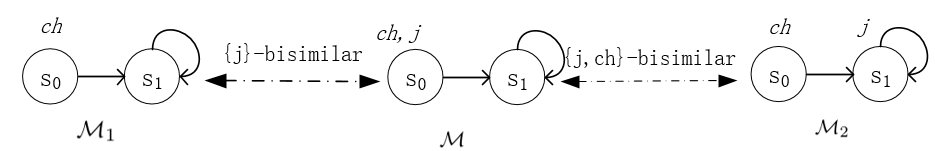
\includegraphics[width=12cm,height=2cm]{figures/chapter06/partial_order.png}
		\caption{初始结构间的$\leq_{\Hm}$关系。}\label{fig:partialo}
		
		% $s_0$ is labeled by $\{ch, j\}$, $t_0$ is labeled by $\{j\}$, and $s_1$, $s_2$, and $t_1$ are labeled by $\emptyset$.}\label{fig:bisim}
	\end{figure}
\end{example}

给定有限初始结构集$M$和有限初始结构$\Hm$,用$Min(M,$ $\leq_{\Hm})$表示$M$中关于偏序关系$\leq_{\Hm}$的极小有限初始结构集。则$\leq_{\Hm}$与知识更新操作$\diamond_{\CTL}$有如下关系。

\begin{theorem}\label{thm:minU}
	给定$\mu$-句子$\Gamma$和$\varphi$,则:
	\[\Mod(\Gamma \diamond_{\CTL} \varphi) = \bigcup_{\Hm\in \Mod(\Gamma)} Min(\Mod(\varphi), \leq_{\Hm}).
	\]
\end{theorem}
\begin{proof}
	$\Hm'\in \Mod(\Gamma \diamond_{\CTL} \varphi)$\\
	$\LRto$ 存在$\Hm \models \Gamma$和极小子集$V_{min} \subseteq \Ha$,使得$\Hm' \in \Mod(\Muforget({\cal F}_{\Ha}(\Hm)$, $V_{min}) \wedge \varphi)$\\
	$\LRto$ 存在$\Hm \models \Gamma$和$V_{min}\subseteq \Ha$,使得$\Hm \lrto_{V_{min}} \Hm'$和$\Hm' \models \varphi$,且$V_{min}$是使得$\Muforget({\cal F}_{\Ha}(\Hm)$, $V_{min}) \wedge \varphi$可满足的$\Ha$极小子集\\
	$\LRto$ 存在$\Hm \models \Gamma$,使得对任意$\Hm''\models \varphi$,$\Hm' \leq_{\Hm} \Hm''$\\
	$\LRto$ $\Hm' \in Min(\Mod(\varphi), \leq_{\Hm})$。
\end{proof}


从定理\ref{thm:minU}可以看出,通过遗忘定义的知识更新操作与通过有限初始结构间的偏序关系定义的知识更新一致,且通过遗忘定义的知识更新操作满足Katsuno和Mendelzon提出的八条基本条件。

\begin{theorem}\label{thm:U1toU8}
	知识更新操作$\diamond_{\CTL}$满足Katsuno和Mendelzon提出的基本条件(U1)-(U8)。
\end{theorem}
\begin{proof}
	(U1). 由定理~\ref{thm:minU}可知,$\Mod(\Gamma \diamond_{\mu} \varphi) \subseteq \Mod(\varphi)$,因此$\Gamma \diamond_{\mu} \varphi \models \varphi$。
	
	(U2). $\Hm'\in \Mod(\Gamma \diamond_{\mu} \varphi)$\\
	$\LRto$ 存在$\Hm \models \Gamma$,使得对任意$\Hm'' \models \varphi$ 和$V \subseteq \Ha$,$\Hm'' \lrto_{V} \Hm$ 蕴涵$\Hm' \lrto_{V} \Hm$\\
	$\LRto$ 存在$\Hm \models \Gamma$和$V_{min} = \emptyset$,使得$\Hm' \lrto_{V_{min}} \Hm$ \hfill ($\Gamma \models \varphi$)\\
	$\LRto$ $\Hm'\models \Gamma$。
	
	
	容易证明$\diamond_{\mu}$满足(U3)和(U4)。
	%We now prove (U5).
	
	(U5). $\Hm'\models (\Gamma \diamond_{\mu} \varphi) \wedge \psi$\\
	$\Rto$  存在$\Hm \models \Gamma$,使得对任意$\Hm'' \models \varphi \wedge \psi$ 和$V \subseteq \Ha$,$\Hm'' \lrto_{V} \Hm$蕴涵$\Hm' \lrto_{V} \Hm$\\
	$\Rto$ 存在$\Hm \models \Gamma$和$V_{min} \subseteq \Ha$,使得$\Hm' \lrto_{V_{min}} \Hm$和$\Hm' \models \varphi \wedge \psi$,其中$V_{min}$是使得$\Hm' \lrto_{V_{min}} \Hm$的$\Ha$的极小子集\\
	% 且对任意的$\Hm''\models \psi$ 若$\Hm''\lrto_V \Hm$则$\Hm' \lrto_{V} \Hm$且$V_{min} \subseteq V$ \\
	$\Rto$ $\Hm' \models \Gamma \diamond_{\mu} (\varphi \wedge \psi)$。
	
	
	
	(U6). $\Hm'\models \Gamma \diamond_{\CTL} \varphi$\\
	$\LRto$ 存在$\Hm \models \Gamma$,使得对任意$\Hm'' \models \varphi$ 和$V \subseteq \Ha$,$\Hm'' \lrto_{V} \Hm$ 蕴涵$\Hm' \lrto_{V} \Hm$\\
	$\LRto$ 存在$\Hm \models \Gamma$和$V_{min} \subseteq \Ha$,使得$\Hm' \lrto_{V_{min}} \Hm$,其中$V_{min}$是使得$\Muforget({\cal F}_{\Ha}(\Hm_1), V_{min}) \wedge \varphi$ 和 $\Muforget({\cal F}_{\Ha}(\Hm_1), V_{min}) \wedge \psi$是一致的 \hfill ($\Gamma \diamond_{\CTL} \varphi \models \psi$, $\Gamma \diamond_{\CTL} \psi \models \varphi$) \\ % \qquad \qquad \textcolor[RGB]{0,134,139}{$\%$({\em Otherwise, suppose that $V\subset V_{min}$ s.t. $\Muforget({\cal F}_{\Ha}(\Hm_1), V) \wedge \psi$ is consistent as well. Then, $\Muforget({\cal F}_{\Ha}(\Hm_1), V)$ $\wedge \varphi$ should also be consistent by $\Gamma \diamond_{\CTL} \varphi \models \psi$, which contradicts to the fact that $V_{min}$ is the minimal set of atoms s.t. $\Muforget({\cal F}_{\Ha}(\Hm_1), V_{min}) \wedge \varphi$ is consistent.})} \\
	$\LRto$ 存在$\Hm \models \Gamma$,使得对任意$\Hm'' \models \psi$ 和$V \subseteq \Ha$,$\Hm'' \lrto_{V} \Hm$ 蕴涵$\Hm' \lrto_{V} \Hm$\\
	$\LRto$ $\Hm' \models \Gamma \diamond_{\CTL} \psi$。
	
	
	
	(U7). $\Hm' \models (\Gamma \diamond_{\CTL} \varphi) \wedge (\Gamma \diamond_{\CTL} \psi)$,且设$\Hm$是$\Gamma$的唯一模型\\
	$\Rto$ 存在两个极小子集$V_1, V_2 \subseteq \Ha$,使得$\Hm \lrto_{V_1} \Hm'$ 和$\Hm \lrto_{V_2} \Hm'$\\
	$\Rto$ 存在两个极小子集$V_1, V_2 \subseteq \Ha$,使得$\Hm' \models \Muforget({\cal F}_{\Ha}(\Hm), V_1) \wedge \varphi$ 和 $\Hm' \models \Muforget({\cal F}_{\Ha}(\Hm),$ $V_2) \wedge \psi$是一致的\\
	%$\Rto$ $\Hm' \lrto_{V_1 \cap V_2} \Hm$\\
	$\Rto$ $\Hm' \models \Muforget({\cal F}_{\Ha}(\Hm), V_1 \cap V_2)$,$\Hm' \lrto_{V_1 \cap V_2} \Hm$,$V_1 = V_2$\\
	$\Rto$  $V_1$是使得$\Muforget({\cal F}_{\Ha}(\Hm), V_1) \wedge (\varphi \vee \psi)$可满足的极小子集\\ %\qquad  \textcolor[RGB]{0,134,139}{$\%$({\em Otherwise, suppose that $V_3\subset V_1$ s.t. $\Muforget({\cal F}_{\Ha}(\Hm),$ $V_3) \wedge (\varphi \vee \psi)$ is satisfiable. Then $\Muforget({\cal F}_{\Ha}(\Hm),$ $V_3) \wedge \varphi$ or $\Muforget({\cal F}_{\Ha}(\Hm),$ $V_3) \wedge \psi$ is satisfiable. Without loss of generality, suppose that $\Muforget({\cal F}_{\Ha}(\Hm), V_3) \wedge \varphi$ is satisfiable, $V_1$ is not the minimal set, a contradiction.})}\\
	$\Rto$ $\Hm' \models \Gamma \diamond_{\CTL} (\varphi \vee \psi)$。
	
	
	
	(U8). $\Hm \models (\Gamma_1 \vee \Gamma_2) \diamond_{\CTL} \varphi$ \\
	$\LRto$ 存在$\Hm_1 \models \Gamma_1$ (或$\Hm_1 \models \Gamma_2$) 和一个极小子集$V_{min}$,使得$\Hm \lrto_{V_{min}} \Hm_1$\\
	$\LRto$ $\Hm \models (\Gamma_1 \diamond_{\CTL} \varphi) \vee (\Gamma_2 \diamond_{\CTL} \varphi)$。
\end{proof}


\begin{example}
	令$\Ha=\{ch, j\}$、$\varphi = \nu X. j \wedge ch \wedge \EXIST \NEXT \EXIST \NEXT X$、 $\psi= \nu X. \neg j \wedge ch \wedge \EXIST \NEXT \EXIST \NEXT X$且Kripke结构的状态空间为 $\{s_0,s_1\}$,则用$\psi$更新$\varphi$计算如下:
	\begin{align*}
		\Mod(\varphi) = & \{((1), r=s_0, L(s_0)=\{ch,j\}, L(s_1)=\{ch,j\}), \\
		& ((2),  r=s_1, L(s_1)=\{ch,j\}, L(s_0)=\{ch,j\}),\\
		& ((3),  r=s_0, L(s_0)=\{ch,j\}, L(s_1)={\cal C}), \\
		& ((4),  r=s_1, L(s_1)=\{ch,j\}, L(s_0)={\cal C}), \\
		& ((5),  r=s_0, L(s_0)=\{ch,j\}, L(s_1)={\cal C}), \\
		& ((6),  r=s_1, L(s_1)=\{ch,j\}, L(s_0)={\cal C}), \dots\}\\
		\Mod(\psi) = & \{((1), r=s_0, L(s_0)=\{ch\}, L(s_1)=\{ch\}),\\
		& ((2), r=s_1, L(s_1)=\{ch\}, L(s_0)=\{ch\}),\\
		& ((3), r=s_0, L(s_0)=\{ch\}, L(s_1)={\cal C}),\\
		& ((4), r=s_1, L(s_1)=\{ch\}, L(s_0)={\cal C}), \\
		& ((5), r=s_0, L(s_0)=\{ch\}, L(s_1)={\cal C}),\\
		& ((6), r=s_1, L(s_1)=\{ch\}, L(s_0)={\cal C}), \dots\}
	\end{align*}
	其中,四元组$((i), r= s_k, L(s_0)=V_1, L(s_1)=V_1)$表示Kripke结构$(S,r,R,L)$,其中$S=\{s_0, s_1\}$、$r=s_k$ ($r\in \{0,1\}$)、转换关系如图~\ref{fig:knoup}中的(i) ($i \in \{1,2,3,4,5,6\}$\footnote{这里只列出部分转换关系,其余转换关系可以容易地枚举出来。})、$s_0$ 和$s_1$分别被 $V_1 \subseteq \{ch,j\}$ 和 $V_2\subseteq \{ch,j\}$标记且${\cal C} \in \{\emptyset, \{j\}, \{ch\}, \{j,ch\}\}$。
	
	$\Mod(\varphi \diamond_{\mu} \psi) = \bigcup_{\Hm\in \Mod(\varphi)} Min(\Mod(\psi), \leq_{\Hm})$,根据定义~\ref{def:closer}容易检查$\Mod(\varphi \diamond_{\mu} \psi) = \Mod(\psi)$。直观地说,由于在$\psi$中$j$在偶数状态不再为真、$ch$保持为真且$\psi$和$\varphi$都不知道模型偶数状态的信息,因而用$\psi$更新$\varphi$得到的结果为 $\psi$自身。
	\begin{figure}[h]%
		\centering
		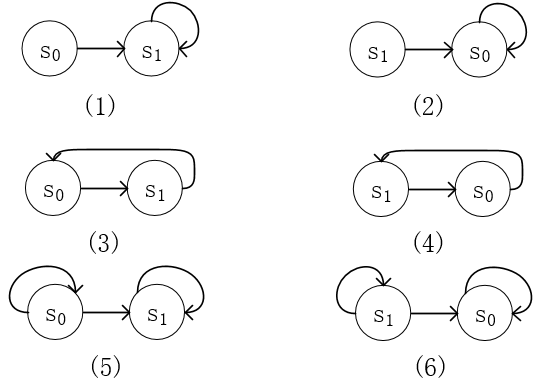
\includegraphics[width=8cm]{knowledge_update.png}
		\caption{状态空间为$\{s_0,s_1\}$的六个Kripke结构示意图}\label{fig:knoup}
		
		% $s_0$ is labeled by $\{ch, j\}$, $t_0$ is labeled by $\{j\}$, and $s_1$, $s_2$, and $t_1$ are labeled by $\emptyset$.}\label{fig:bisim}
	\end{figure}
\end{example}


\section{本章小结}\label{sec:chapter04-conclusion}

本章讨论了如何使用遗忘计算最强必要条件(最弱充分条件)和定义知识更新。特别地,本章首先给出了SNC(WSC)的定义,表明SNC和WSC是一对对偶概念,因而只要知道其一就能知道另一个。其次,结论表明任意公式的SNC(WSC)可以转换成原子命题的SNC(WSC)来计算,并给出使用遗忘计算原子命题在给定条件下的SNC(WSC)的方法。
最后,分别给出使用遗忘和偏序关系的方法定义知识更新,并证明了这两种定义等价且满足Katsuno等人提出的八条准则。

 

\chapter{$\CTL$遗忘计算方法}
\label{chapter05}
{\em 第~\ref{chapter03}章探索了$\CTL$遗忘的定义及其基本性质,本章给出两种计算$\CTL$遗忘的算法:基于模型的算法和基于归结的算法$\CTL$-forget。
	
	基于模型的计算考虑固定有限状态空间下的初始结构。本章证明这样的初始结构可由一个$\CTL$公式来表示,因而其遗忘结果可以由$\CTL$公式表示。

基于归结的计算方法首先将$\CTL$公式转化为$\CTLsnf$子句,然后使用归结系统$R_{\CTL}^{\succ,S}$中的规则对要遗忘的原子命题归结,最后将得到的结果等价转化为$\CTL$公式。
基于此,本章详细介绍了基于Prolog的$\CTL$-forget算法实现,并给出部分实验结果及结果分析。

最后总结本章的主要工作。}

\section{基于模型的有界$\CTL$遗忘计算}
\label{chapter05:sec:model}
	遗忘与均匀插值是一对对偶概念。已有研究表明$\CTL$不具有均匀插值性质~\cite{Maksimova:JANCL:1991},这表明$\CTL$遗忘不是封闭的
	%\footnote{对于给定的逻辑语言${\cal L}$和该语言上的操作${\cal O}$,若$\cal O$作用到$\cal L$中的元素后得到的结果仍然在$\cal L$中,则称$\cal O$在$\cal L$下是封闭的。}
	。
	此时,探索$\CTL$下遗忘封闭的情形对深入应用遗忘有重要意义。
	为此,本章首先提出有限初始结构的特征公式;其次,表明$\CTL$公式的遗忘结果在此情形下可以表示成其模型的特征公式的析取;最后,提出一种基于模型的方法计算遗忘。%,且探索了如何使用遗忘计算最弱充分条件和知识更新。


%系统模型通常是有限的
%小模型理论,公式的长度有限
%描述数(特征数)来区分同意结构内那些状态在一定程度上是相同的,如果超过这个度,肯定不同。此时,就可以使用CTL公式来描述这些状态及其关系。
%描述forgetting的四个规则。



现实情况下能处理的系统都是有限的,且在某一固定环境下所涉及到的原子命题是有限的。因此,在这部分讨论一种约束的$\CTL$,即:
\begin{itemize}
	\item[(1)] 出现在$\CTL$公式中的原子命题的个数是有限的(即$\Ha$是有限的);
	\item[(2)] 初始结构的状态空间$S$是一个有限的固定状态空间${\cal S}=\{b_1,\ldots,b_m\}$的子集(即$S \subseteq {\cal S}$),且使得对于任意约束长度的$\CTL$公式$\varphi$,若$\varphi$是可满足的,则存在一个状态空间是${\cal S}$的子集的初始结构$(\Hm,s_0)$,使得$(\Hm,s_0)\models \varphi$。
\end{itemize}
由此可见,在这种情形下只有有限个初始结构会被考虑。
下文表明在这一约束条件下$\CTL$中的遗忘是封闭的。

本节其余部分组织如下:首先,在第\ref{chapter06:sec:des}节定义有界$V$-互模拟,然后定义初始结构的特征公式;其次,在第\ref{chapter06:sec:close}节证明约束$\CTL$下的遗忘是封闭的,并给出计算方法;最后,在第\ref{chapter06:sec:algm}节给出基于模型的计算遗忘的算法,并分析算法的复杂性。


\subsection{描述初始结构}\label{chapter06:sec:des}%\label{sec:chapter06_chaIntC}
本小节介绍与一个初始结构相关的$\CTL$公式——特征公式。
%对于一个给定的有限初始结构(状态个数和$\Ha$都是有限的),其不循环的计算树(状态不重复出现)的深度最多为其状态数的个数。
对于一个给定的初始结构,其特征公式与其计算树的特征公式密切相关。
因此,本小节首先介绍计算树之间的$V$-互模拟关系;然后,给出计算树的特征公式的定义;最后,给出初始结构的特征公式。

\subsubsection{计算树$V$-互模拟}
第\ref{chapter03}章中的定义\ref{def:VInd:bisimulation}给出了$\Ind$-结构之间的$V$-互模拟定义及其相关性质,结构之间的$V$-互模拟有相同的定义,即:$\Ind$-结构之间$V$-互模拟具有的性质都可以平凡的迁移到结构之间$V$-互模拟。
这里给出有限结构间有界$V$-互模拟(与深度$n$关联的$V$-互模拟)的定义,并证明$V$-互模拟与有界$V$-互模拟在有限结构下等价。
%本节给出结构之间的$V$-互模拟在有限结构下与下面将要给出的有界$V$-互模拟——与深度$n$关联的$V$-互模拟等价。
%但是为了方便,本章仍然引入有界$V$-互模拟的概念。
因此,第\ref{chapter03}章遗忘有的性质在本章约束情形下基本也有~\cite{renyansfirstpaper},这里不再赘述。

首先给出能够描述一定深度$n\in \mathbb{N}$的计算树之间的$V$-互模拟关系,记为$\Hb_n^V$。令$V\subseteq \Ha$是原子命题集,$i\in \{1,2\}$,$\Hm_i=(S_i,R_i,L_i,s_0^i)$是初始Kripke结构,${\cal K}_i=(\Hm_i, s_i)$是结构。$\Hb_n^V$递归定义如下:
\begin{itemize}
	\item 若$L_1(s_1)-V=L_2(s_2)$,则$({\cal K}_1,{\cal K}_2) \in \Hb_0^V$;
	\item 对任意$n\ge 0$,若满足下面几个条件,则$({\cal K}_1,{\cal K}_2)\in \Hb_{n+1}^V$成立:
	\begin{itemize}
		\item $({\cal K}_1,{\cal K}_2) \in \Hb_0^V$;
		\item 对任意$(s_1,s_1')\in R_1$,存在$(s_2,s_2')\in R_2$,使得$({\cal K}_1',{\cal K}_2') \in \Hb_n^V$;
		\item 对任意$(s_2,s_2')\in R_2$,存在$(s_1,s_1')\in R_1$,使得$({\cal K}_1',{\cal K}_2') \in \Hb_n^V$。
	\end{itemize}
\end{itemize}
其中${\cal K}_i'=(\Hm_i,s_i')$。

当所谈及的原子命题集$V$很显然的时候,上述$\Hb_n^V$中的$V$可以省略,记为$\Hb_n$。此外,当讨论的$\Hm_i$ $(i=1,2)$是显然的时候,可以使用$(s_1,s_2) \in \Hb_n$代替$((\Hm_1,s_1),(\Hm_2,s_2))$ $\in \Hb_n$。
有界$V$-互模拟关系就可以定义如下:
\begin{definition}[有界$V$-互模拟]\label{def:V-bisimulation}
	令$V$是$\Ha$的一个子集,$i\in \{1,2\}$, ${\cal K}_1$和${\cal K}_2$是结构。
	\begin{itemize}
		\item ${\cal K}_1$和${\cal K}_2$是有界$V$-互模拟的,当且仅当对所有$n \ge 0$,都有$({\cal K}_1, {\cal K}_2)\in \Hb_n$。若 ${\cal K}_1$ 和 ${\cal K}_2$是有界$V$-互模拟的,则记为${\cal K}_1 \overset{B}{\lrto}_V {\cal K}_2$。
		\item 对$\Hm_i$上的路径$\pi_i=(s_{i,1},s_{i,2},\dots)$,若对于任意$j\in \mathbb{N}_{\ge 1}$\footnote{$\mathbb{N}$为整数集,$\mathbb{N}_{\ge 1}$是大于等于1的整数集。},都有${\cal K}_{1,j} \overset{B}{\lrto}_V {\cal K}_{2,j}$,则$\pi_1 \overset{B}{\lrto}_V \pi_2$。其中${\cal K}_{i, j}=(\Hm_i, s_{i,j})$。
	\end{itemize}
\end{definition}

值得注意的是,满足有界$V$-互模拟关系的结构之间有且仅有一个有界$V$-互模拟关系,即$\Hb_{k+1} = \Hb_k$($k \in \mathbb{N}$)。
%上述约束$V$-互模拟的定义是现有互模拟定义的一般化,这可以从下面几个方面来体现\footnote{在其他领域也有类似的定义,如:定义在数据库相关文献中的概念$k$-互模拟\cite{kaushik2002updates}。$k$-互模拟概念中涉及与本文$\Hb_n$类似的定义,只是其关系是从相反的方向(即:从孩子到父节点的方向)来说明的。此外,值得一提的是,本文的$V$-互模拟的概念是定义在$\MPK$-结构上的。}。
%首先,当给定的$V$为空集且谈论指定的初始状态时,本文的$V$-互模拟与定义在Baier等文章里的互模拟等价(定义7.1\cite{Baier:PMC:2008})的概念一致。
%其次,在上述文章里的基于状态的互模拟(定义7.7\cite{Baier:PMC:2008})是定义在给定结构的状态上的,因此与本文的$V$-互模拟(定义在结构的集合上)也不同。
%最后,本文的$\Hb_n$的定义与Browne的论文中的状态等价$E_n$类似,只是后者是定义在状态上\cite{browne1988characterizing}而本文的定义在$\MPK$-结构(或$\Ind$-结构)上。


\begin{lemma} \label{lem:HbBis}
	对于有限初始Kripke结构,有界 $V$-互模拟是一个 $V$-互模拟。
	%Let $V \subseteq \Ha$ and ${\cal K}_i=({\cal M}_i,s_i)~(i\in\{1,2\})$ and $\Hm_i=(S_i, R_i,L_i, s_0^i)$ be finite initial structures. 
	%Then every bounded $V$-bisimulation is a $V$-bisimulation between $\Hm_1$ and $\Hm_2$.
	%If $s_1 \lrto_V s_2$, then the bounded $V$-bisimulation {\cal B}_V containing $(s_1, s_2)$ is also a $V$-bisimulation (containing $(s_1,s_2)$) between $\Hm_1$ and $\Hm_2$.
\end{lemma}

\begin{proof}
	令 $V \subseteq \Ha$、 ${\cal K}_i=({\cal M}_i,s_i)~(i\in\{1,2\})$且$\Hm_i=(S_i, R_i,L_i, s_0^i)$为有限的初始-Kripke结构。
	因为$S_i~(i=1,2)$是有限的,所以$\Hb_n\subseteq S_1\times S_2~(n\ge 0)$都是有限的。
	由于对任意$n\geq 0$,都有 $\Hb_{n+1} \subseteq \Hb_n$。
	因此,存在一个最小数$k$,使得
	$\Hb_{k+1} =\Hb_k$(用 $\Hb$表示)。
	
	
	下证对任意 $r_1\in S_1$和 $r_2 \in S_2$,若$(r_1, r_2)\in \Hb$,则 %if and only if
	\begin{itemize}
		\item[(a)] $L_1(r_1)-V = L_2(r_2)-V$;
		\item[(b)] $\forall w_1\in S_1$,若$(r_1, w_1)\in R_1$,则 $\exists w_2 \in S_2$,使得 $(r_2,w_2) \in R_2$和 $(w_1, w_2) \in \Hb$;
		\item[(c)] $\forall w_2\in S_2$,若$(r_2, w_2)\in R_2$,则 $\exists w_1 \in S_1$,使得 $(r_1,w_1) \in R_1$和 $(w_1, w_2)\in \Hb $。
	\end{itemize}
	
	首先,由对任意$n\ge 0$,都有$(r_1, r_2)\in \Hb_n$,可知$(r_1, r_2) \in \Hb_0$,这表明
	$L_1(r_1)-V = L_2(r_2)-V$。因此(a)成立。
	
	其次,令$w_1 \in S_1$和 $(r_1, w_1)\in R_1$。有 \\
	$(r_1,r_2)\in \Hb$、 $w_1 \in S_1$和 $(r_1, w_1)\in R_1$\\
	$\Rto$ 由$\Hb_{k+1}=\Hb$可知$(r_1,r_2)\in \Hb_{k+1}$、 $w_1 \in S_1$和 $(r_1, w_1)\in R_1$\\
	$\Rto$ 由定义可知$\exists w_2\in S_2$,使得 $(r_2, w_2)\in R_2$和 $(w_1,w_2)\in \Hb_k$\\
	$\Rto$ 由$\Hb=\Hb_k$可知$\exists w_2\in S_2$,使得 $(r_2, w_2)\in R_2$和 $(w_1,w_2)\in \Hb$\\
	$\Rto$ (b)成立。
	
	可以类似地证明 (c)也成立。
	因此, $\Hb$是$\Hm_1$和 $\Hm_2$之间的一个 $V$-互模拟关系。
\end{proof}

由引理\ref{lem:HbBis}可知,$\Hb$既是一个有界$V$-互模拟关系也是一个$V$-互模拟关系。因此,下面的推论显然成立。
\begin{corollary} \label{lem:bounedToGe}
	令 $V \subseteq \Ha$ 和 ${\cal K}_i=({\cal M}_i,s_i)$( $i\in\{1,2\}$)。若$\Hm_i=(S_i, R_i,L_i, s_0^i)$是有限的初始Kripke结构,则
	%$s_1 \overset{\Hb}{\lrto}_V s_2$ 
	$s_1$和 $s_2$是有界 $V$-互模拟的,当且仅当$s_1 \lrto_V s_2$。
\end{corollary}


本章只涉及有限的初始Kripke结构,因此,本章用$\lrto_V$($V$-互模拟)表示$\overset{B}{\lrto}_V $(有界$V$-互模拟)。

给定原子命题集$V\subseteq \Ha$和初始Kripke结构$\Hm_i$($i = 1, 2$)。如果下面条件同时满足:
\begin{itemize}
	\item $L_1(s_1)- V=L_2(s_2)- V$,
	%   \item For every subtree $\Tr_{n-1}(s_i')$ of $\Tr_n(s_i)$,
	%   $\Tr_n(s_{(i \mod 2)+1})$ has a subtree $\Tr_{n-1}(s_{(i \mod 2)+1}')$ such that
	%   $\Tr_{n-1}(s_i')\lrto_V\Tr_{n-1}(s_{(i \mod 2)+1}')$.
	\item 对$\Tr_n(s_1)$的任意子树$\Tr_{n-1}(s_1')$,都存在  $\Tr_n(s_2)$的子树$\Tr_{n-1}(s_2')$,使得 
	$\Tr_{n-1}(s_1')\lrto_V\Tr_{n-1}(s_2')$,且
	\item 对任意$\Tr_n(s_2)$的子树$\Tr_{n-1}(s_2')$,都存在$\Tr_n(s_1)$的子树$\Tr_{n-1}(s_1')$,使得
	$\Tr_{n-1}(s_1')\lrto_V\Tr_{n-1}(s_2')$;
\end{itemize}
则称$\Hm_1$的计算树$\Tr_n(s_1)$和$\Hm_2$的计算树$\Tr_n(s_2)$是$V$-互模拟的(记为$({\cal M}_1,\Tr_n(s_1))\lrto_V({\cal M}_2,\Tr_n(s_2))$,简写为$\Tr_n(s_1)\lrto_V\Tr_n(s_2)$)

特别地,当$n=0$时,只需考虑第一个条件即可。

\begin{proposition}\label{B_to_T}
	给定原子命题集$V\subseteq\cal A$和结构$({\cal M}_i,s_i)$($i=1,2$)。
	那么:
	\[(s_1,s_2)\in{\cal B}_n\mbox{当且仅当对任意$0\le j\le n$,有}
	\Tr_j(s_1)\lrto_V\Tr_j(s_2)\mbox{。}\]
\end{proposition}
\begin{proof}
	下面从两个方面来证明这一结论。
	
	$(\Rto)$ 下证“如果$(s_1, s_2) \in \Hb_n$,则对于任意$0 \leq j \leq n$,有$Tr_j(s_1) \lrto_V Tr_j(s_2)$”成立。$(s_1, s_2) \in \Hb_n$表明$Tr_n(s_1)$和$Tr_n(s_2)$的根有同样的标签(除了$V$里的元素之外)。
	此外,对任意$(s_1, s_{1,1}) \in R_1$,存在一个$(s_2, s_{2,1})\in R_2$,使得$(s_{1,1}, s_{2,1}) \in \Hb_{n-1}$;且对任意$(s_2, s_{2,1})\in R_2$,存在一个$(s_1, s_{1,1}) \in R_1$,使得$(s_{1,1}, s_{2,1}) \in \Hb_{n-1}$。
	因此,由定义可知$Tr_1(s_1)$ $\lrto_V Tr_1(s_2)$。递归地使用上述方法可得对任意$0 \leq j \leq n$,都有$Tr_j(s_1) \lrto_V Tr_j(s_2)$。
	
	$(\Lto)$下证“如果对于任意$0 \leq j \leq n$有$Tr_j(s_1) \lrto_V Tr_j(s_2)$,则$Tr_j(s_1) \lrto_V Tr_j(s_2)$”成立。
	由$Tr_0(s_1) \lrto_V Tr_0(s_2)$可知$L(s_1) - V = L'(s_2) - V$,因而$(s_1, s_2) \in \Hb_0$。
	由$Tr_1(s_1) \lrto_V Tr_1(s_2)$可知$L(s_1) - V = L'(s_2)- V$,且对于一棵树根的任意后继状态$s$,都能找到另一棵树根的一个后继状态$s'$,使得$(s, s')\in \Hb_0$。
	因此,$(s_1, s_2) \in \Hb_1$。同理可证$(s_1, s_2) \in \Hb_2$, \dots, $(s_1, s_2) \in \Hb_n$。
\end{proof}

命题\ref{B_to_T}表明,任意两个初始结构中的两个状态$s_1$和$s_2$能够在$\overline{V}$上相互模拟对方直到$n$步,当且仅当分别以$s_1$和$s_2$为根的计算树能在$\overline{V}$上相互模拟直到深度为$n$。
由此可知,如果同一初始结构的两个状态$s$和$s'$不是$V$-互模拟的,则存在一个数$k\in \mathbb{N}$,使得分别以$s$和$s'$为根的计算树$\Tr_k(s)$和$\Tr_k(s')$不是$V$-互模拟的。
\begin{proposition}\label{pro:k}
	给定原子命题集$V\subseteq \Ha$、初始Kripke结构$\Hm$和两个状态$s,s'\in S$。
	若$s\not\lrto_V s'$,则存在一个最小整数$k$,使得$\Tr_k(s)$和$\Tr_k(s')$不是$V$-互模拟的。
\end{proposition}
\begin{proof}
	若$s\not\lrto_V s'$,则存在一个最小的数$c$,使得$(s_i, s_j) \notin \Hb_c$。因此,由命题\ref{B_to_T}可知,存在一个最小整数$m$($m \leq c$),使得$\Tr_m(s_i)$和 $\Tr_m(s_j)$不是$V$-互模拟的。令$k=m$可得上述结论。
\end{proof}


\subsubsection{计算树的特征公式}
由上面小节的讨论可知,$V$-互模拟可以将计算树区别开\footnote{相似的方法在Mycielski等人的文章中已被使用~\cite{DBLP:conf/birthday/1997ehrenfeucht},在这篇文章中一元公式的结构通过等价类$\equiv_{\overline{k}}$被描述为Hintikka公式~\cite{hintikka1953distributive}。另一个类似的工作是Yankov-Fine构造~\cite{yankov1968three}。}。下面讨论如何使用$\CTL$公式描述计算树,且表明具有(或没有)$V$-互模拟关系的计算树的特征公式之间的关系。为此,首先给出计算树特征公式的定义。
\begin{definition}\label{def:V:char:formula}
	给定原子命题集$V\subseteq \Ha$、初始Kripke结构$\Hm =(S,R,L,s_0)$和状态$s\in S$。
	定义在$V$上的计算树$\Tr_n(s)$的特征公式(记为${\cal F}_V(\Tr_n(s))$,$n\geq 0$)递归定义如下:
	\begin{align*}
		{\cal F}_V(\Tr_0(s)) &=  \bigwedge_{p \in V\cap L(s)}p
		\wedge \bigwedge_{q\in V-L(s)} \neg q,\\
		{\cal F}_V(\Tr_{k+1}(s))& = \bigwedge_{(s,s')\in R}
		\EXIST \NEXT {\cal F}_V(\Tr_k(s')) 
		\wedge 
		\ALL \NEXT \bigg( \bigvee_{(s,s')\in R} {\cal F}_V(\Tr_k(s')) \bigg) \wedge {\cal F}_V(\Tr_0(s)) \hbox{ ($k\ge 0$)。}
	\end{align*}
\end{definition}

由定义\ref{def:V:char:formula}可知,计算树的特征公式从三个方面展示了计算树的信息:
\begin{itemize}
	\item[(1)] 只考虑$V$中的原子命题;
	\item[(2)] 突出了树节点的内容,即:对于任意原子命题$p\in V$,若$p$在节点的标签中,则其正出现在特征公式中,否则负出现在特征公式中;
	\item[(3)] 公式中的时序算子表示了状态之间的转换关系。
\end{itemize}
通俗一点,${\cal F}_V(\Tr_0(s))$表明了节点$s$的在$V$上的内容;$\EXIST \NEXT$的合取部分和$\ALL \NEXT$部分保证,以$s$的每个直接后继状态$s'$为根、深度为$k$的计算树都有一个$\CTL$公式来描述。

下面的结论表明,若两个计算树是$V$-互模拟的,则它们在$V$上的特征公式是逻辑等价的。
\begin{lemma}\label{lem:Vb:TrFormula:Equ}
	给定原子命题集$V\subseteq \Ha$、初始Kripke结构$\Hm=(S,R,L,s_0)$和$\Hm'=(S',R',L',s_0')$、$s\in S$、$s'\in S'$且 $n\ge 0$。若$\Tr_n(s) \lrto_{\overline V} \Tr_n(s')$,则${\cal F}_V(\Tr_n(s)) \equiv {\cal F}_V(\Tr_n(s'))$。
\end{lemma}
\begin{proof}
	通过归纳计算树的深度$n$来证明。
	
	\textbf{基始($n=0$):} 对任意$s_x\in S$和$s_x' \in S'$,若$\Tr_0(s_x) \lrto_{\overline V} \Tr_0(s_x')$,则由$L(s_x) - \overline V = L'(s_x') - \overline V$可知${\cal F}_V(\Tr_0(s_x)) \equiv {\cal F}_V(\Tr_0(s_x'))$。
	
	\textbf{归纳步($n>0$):} 假设对任意$0\leq m \leq n$,若$\Tr_m(s) \lrto_{\overline V} \Tr_m(s')$,则${\cal F}_V(\Tr_m(s)) \equiv {\cal F}_V(\Tr_m(s'))$。
	下证若$\Tr_{n+1}(s) \lrto_{\overline V} \Tr_{n+1}(s')$,则${\cal F}_V(\Tr_{n+1}(s)) \equiv {\cal F}_V(\Tr_{n+1}(s'))$。
	
	由归纳假设可知,对任意$k=m$、$s_k\in S$和$s_k'\in S'$,若$\Tr_{n-k}(s_k) \lrto_{\overline V} \Tr_{n-k}(s_k')$,则 ${\cal F}_V($ $\Tr_{n-k}(s_k)) \equiv {\cal F}_V(\Tr_{n-k}(s_k'))$。
	因此,要证原结论成立,只需要证明:若$\Tr_{n-k+1}(s_{k-1})$ $\lrto_{\overline V} \Tr_{n-k+1}(s_{k-1}')$,则${\cal F}_V(\Tr_{n-k+1}(s_{k-1})) \equiv {\cal F}_V(\Tr_{n-k+1}(s_{k-1}'))$。其中,$(s_{k-1},$ $s_k)\in R$且$(s_{k-1}',$ $s_k')\in R'$。
	显然,由计算树的特征公式可知:
	\begin{align*}
		{\cal F}_V(\Tr_{n-k+1}(s_{k-1})) &  =
		\left(\bigwedge_{(s_{k-1},s_k)\in R}
		\EXIST \NEXT {\cal F}_V(\Tr_{n-k}(s_k))\right)
		\wedge \\
		&\ALL \NEXT\left(\bigvee_{(s_{k-1},s_k)\in R}
		{\cal F}_V(\Tr_{n-k}(s_k) )\right)
		\wedge {\cal F}_V(\Tr_0(s_{k-1}))
	\end{align*}
	且
	\begin{align*}
		{\cal F}_V(\Tr_{n-k+1}(s_{k-1}')) &  =
		\left(\bigwedge_{(s_{k-1}',s_k')\in R}
		\EXIST \NEXT {\cal F}_V(\Tr_{n-k}(s_k'))\right)
		\wedge \\
		&\ALL \NEXT\left(\bigvee_{(s_{k-1}',s_k')\in R}
		{\cal F}_V(\Tr_{n-k}(s_k') )\right)
		\wedge {\cal F}_V(\Tr_0(s_{k-1}')).
	\end{align*} 
	
	又因为$\Tr_{n-k+1}(s_{k-1})$ $\lrto_{\overline V} \Tr_{n-k+1}(s_{k-1}')$,所以,对任意$(s_{k-1}, s_k) \in R$,存在$(s_{k-1}', s_k') \in R'$,使得$\Tr_{n-k}(s_k) \lrto_{\overline V} \Tr_{n-k}(s_k')$,且对任意$(s_{k-1}', s_k') \in R'$,存在$(s_{k-1}, s_k) \in R$,使得$\Tr_{n-k}(s_k)$ $ \lrto_{\overline V}\Tr_{n-k}(s_k')$。
	因此,由归纳假设可知${\cal F}_V(\Tr_{n-k+1}(s_{k-1})) \equiv {\cal F}_V(\Tr_{n-k+1}(s_{k-1}'))$。
\end{proof}

此外,对于初始Kripke结构$\Hm$上的状态$s$和$s'$,若$(\Hm,s)$是定义在$V$上、根为$s'$、深度为$n$的计算树特征公式的模型,则$s$和$s'$至少属于$\Hb_n$,即:$s$和$s'$能相互模拟至少到第$n$层深度。

\begin{lemma}\label{Bn:to:Tn}
	令$V\subseteq \Ha$、$\Hm=(S, R, L,s_0)$、$\Hm'=(S', R', L',s_0')$、$s\in S$、$s'\in S'$且$n\ge 0$,则:
	\begin{itemize}
		\item[(i)] $({\cal M},s)\models{\cal F}_V(\Tr_n(s))$;
		\item[(ii)] 若$({\cal M},s)\models{\cal F}_V(\Tr_n(s'))$,则
		$\Tr_n(s) \lrto_{\overline V} \Tr_n(s')$。
	\end{itemize}
\end{lemma}
\begin{proof}
	(i) \textbf{基始($n=0$):}从树的特征公式定义可知$L(s) \models {\cal F}_V(\Tr_0(s))$,所以,$({\cal M},s)\models{\cal F}_V(\Tr_n(s))$。
	
	\textbf{归纳步($n>0$):} 假设对任意$k\geq 0$,$({\cal M},s)\models{\cal F}_V(\Tr_k(s))$,下面证明$({\cal M},s)\models{\cal F}_V(\Tr_{k+1}(s))$,即:
	\begin{equation*}
		({\cal M},s)\models \left(\bigwedge_{(s,s')\in R}
		\EXIST \NEXT T(s')\right)
		\wedge \ALL \NEXT\left(\bigvee_{(s,s')\in R}
		T(s')\right)
		\wedge {\cal F}_V(\Tr_0(s)).
	\end{equation*}
	其中$T(s') ={\cal F}_V(\Tr_k(s'))$。 
	由基始可知$({\cal M},s)\models {\cal F}_V(\Tr_0(s))$。
	由归纳假设可知,对任意$(s,s') \in R$,有$({\cal M}, s') \models {\cal F}_V(\Tr_k(s'))$。因此,$({\cal M},s)\models \EXIST \NEXT {\cal F}_V(\Tr_k(s')$,从而$({\cal M},s)\models \bigwedge_{(s,s')\in R}
	\EXIST \NEXT {\cal F}_V(\Tr_k(s'))$。
	
	同理,对任意$(s,s') \in R$,都有$({\cal M}, s') \models \bigvee_{(s,s')\in R} {\cal F}_V(\Tr_k(s') )$。因此,
	$$({\cal M},s)\models \ALL \NEXT\left(\bigvee_{(s,s')\in R}
	{\cal F}_V(\Tr_k(s') )\right)$$
	
	所以,对任意$n\geq 0$,$({\cal M},s)\models{\cal F}_V(\Tr_n(s))$。
	
	
	
	(ii) \textbf{基始($n=0$):}若$(\Hm, s)  \models {\cal F}_V(\Tr_0(s'))$,则$L(s) - \overline V = L'(s') - \overline V$。因此,$\Tr_0(s) \lrto_{\overline V} \Tr_0(s')$。
	
	\textbf{归纳步($n>0$):} 假定若$({\cal M},s)\models{\cal F}_V(\Tr_{n-1}(s'))$,则$\Tr_{n-1}(s) \lrto_{\overline V} \Tr_{n-1}(s')$。下证若$({\cal M},s)\models{\cal F}_V(\Tr_n(s'))$,则
	$\Tr_n(s) \lrto_{\overline V} \Tr_n(s')$。
	
	\begin{itemize}
		\item[(a)] 由基始知$L(s) - \overline V = L'(s') - \overline V$;
		\item[(b)] 因为$(\Hm, s) \models {\cal F}_V(\Tr_n(s'))$,所以,$(\Hm, s) \models \ALL \NEXT\left(\bigvee_{(s',s_1')\in R}{\cal F}_V(\Tr_{n-1}(s_1') )\right)$。所以,对于任意$(s, s_1) \in R$,存在$(s', s_1') \in R'$,使得$(\Hm, s_1) \models {\cal F}_V(\Tr_{n-1}(s_1') )$。由归纳假设可知$\Tr_{n-1}(s_1) \lrto_{\overline V} \Tr_{n-1}(s_1')$。即:$\forall (s, s_1) \in R$,$\exists (s', s_1') \in R'$,使得$\Tr_{n-1}(s_1) \lrto_{\overline V} \Tr_{n-1}(s_1')$。
		
		\item[(c)] 因为$(\Hm, s) \models {\cal F}_V(\Tr_n(s'))$,所以,$(\Hm, s) \models  \bigwedge_{(s',s_1')\in R'} \EXIST \NEXT {\cal F}_V(\Tr_{n-1}(s_1'))$。对任意$(s',$ $s_1')\in R'$,存在$(s,s_1)\in R$,使得$(\Hm, s_1) \models {\cal F}_V(\Tr_{n-1}(s_1')$。由归纳假设可知$\Tr_{n-1}(s_1)$ $\lrto_{\overline V} \Tr_{n-1}(s_1')$,即:$\forall (s',s_1')\in R'$,$\exists (s,s_1)\in R$,使得$\Tr_{n-1}(s_1) \lrto_{\overline V} \Tr_{n-1}(s_1')$。
	\end{itemize}
\end{proof}

\subsubsection{初始结构的特征公式}
由$V$-互模拟的定义和命题\ref{pro:k}可以自然地得到一个$V$-互模拟的补概念——$V$-可区分。
特别地,在命题\ref{pro:k}中,若初始Kripke结构$\Hm$的两个状态$s$和$s'$不是$\overline{V}$-互模拟的(即:$s\not\lrto_{\overline{V}} s'$),则称$s$和$s'$是\emph{$V$-可区分的}。
用$\dis_V({\cal M},s,s',k)$表示状态$s$和$s'$在命题\ref{pro:k}中所说的最小数$k$下是$V$-可区分的。
%正如下文所说,$V$-可区分这一概念是定义初始结构特征公式的重要概念。

此外,对于给定的初始Kripke结构$\Hm$和原子命题集$V$,若在$\Hm$中存在两个状态$s$和$s'$是$V$-可区分的,则称$\Hm$是$V$-可区分的。
而对于一个$V$-可区分的初始Kripke结构$\Hm$,存在一个最小数$k$,使得对于该结构上的任意两个状态$s$和$s'$,若$s$和$s'$是可区分的,则$(s,s')\not \in \Hb_k$。本文称这样的数为$\Hm$关于$V$的\emph{特征数},记为$ch({\cal M},V)$,其定义如下:
\[ch({\cal M},V)=
\left\{
\begin{array}{ll}
	\max\{k\mid s,s'\in S \text{ 且 }\dis_V({\cal M},s,s',k)\}, \qquad \hbox{${\cal M}$是 $V$-可区分的;} \\
	\min\{k\mid {\cal B}_{k}={\cal B}_{k+1}, k\ge 0\}, \ \ \ \quad  \qquad \qquad \qquad \hbox{否则。}
\end{array}
\right.
\]

由$ch({\cal M},V)$定义可知,对于任意$\Hm$和$V$,$ch({\cal M},V)$总是存在的,这体现在两个方面:
\begin{itemize}
	\item[(1)] 若$\Hm$是$V$-可区分的,则存在两个状态$s$和$s'$是$V$-可区分的,由命题\ref{pro:k}可知,存在一个数$k$,使得$\dis_V({\cal M},s,s',k)$成立;
	\item[(2)] 若对于任意$k\geq 0$和$\Hm$上的两个状态$s$和$s'$,都有$(s,s')\in \Hb_k$且$\Hb_k =\Hb_{k+1}$,则$ch({\cal M},$ $V)=0$。
\end{itemize}

直观上,特征数$c=ch({\cal M},V)$将$\Hm$上的状态分为两大类:第一类中的任意两个状态$s$和$s'$是$V$-可区分的,且$(s,s')\not \in \Hb_c$;第二类中的状态都是$V$-不可区分的。%这也在计算树的特征公式上:

\begin{lemma}\label{div_s}
	令$V\subseteq \Ha$、$\Hm=(S,R,L,s_0)$、$k={ch({\cal M},V)}$且$s\in S$,则
	%There is a formula $\phi$ such that
	\begin{itemize}
		\item[(i)] $(\Hm, s)\models {\cal F}_V(\Tr_k(s))$;
		\item[(ii)] 对任意$s'\in S$,$({\cal M},s) \lrto_{\overline V} ({\cal M},s')$当且仅当$({\cal M},s')\models{\cal F}_V(\Tr_k(s))$。
	\end{itemize}
\end{lemma}
\begin{proof}
	(i) 这由引理\ref{Bn:to:Tn}易知。
	
	(ii) 令$\phi = {\cal F}_V(\Tr_k(s))$($k$为$\Hm$关于$V$的特征数)。由(i)可知 $(\Hm, s) \models \phi$,从而对任意$s' \in S$,若$s \lrto_{\overline V} s'$,由定理\ref{thm:V-bisimulation:EQ}和$\IR(\phi, \Ha - V)$可知$(\Hm, s') \models \phi$。
	
	假定$(\Hm, s')\models \phi$。若$s \nleftrightarrow_{\overline V} s'$,则$\Tr_k(s) \not \lrto_{\overline V} \Tr_k(s')$,因而由引理\ref{Bn:to:Tn}可知$(\Hm, s')\not \models \phi$,这与假定矛盾。
\end{proof}

由此,可如下定义初始结构的特征公式。

\begin{definition}[特征公式]
	给定原子命题集$V\subseteq\cal A$和初始结构${\cal K}=({\cal M},s_0)$,其中$c=ch({\cal M},V)$。对任意$\Hm$上的状态$s' \in S$,记$T(s') = {\cal F}_V(\Tr_c(s'))$。
	$\cal K$关于$V$的{\em 特征公式} ${\cal F}_V({\cal K})$定义为:
	\[T(s_0) \text{ } \wedge \bigwedge_{s\in S}\ALL \GLOBAL\left(
	T(s) \rto
	\bigwedge_{(s,s')\in R}
	\EXIST \NEXT T(s')
	\wedge
	\ALL \NEXT \bigg(\bigvee_{(s,s')\in R}T(s')\bigg)
	\right).
	\]
	
\end{definition}

有时为了凸显出初始Kripke结构及其初始状态,也把特征公式写为${\cal F}_V(\Hm, s_0)$。显然,$\IR({\cal F}_V(\Hm, s_0), \overline V)$。此外,在特征公式的定义中,使用了深度为$c$(即:特征数)的计算树的特征公式:意在表明对任意$\Hm$上的两个状态$s$和$s'$,$s$和$s'$是$V$-可区分的当且仅当${\cal F}_V(\Tr_c(s))\not \equiv {\cal F}_V(\Tr_c(s'))$。特别地,$T(s)$确保了状态$s\in S$被$\CTL$公式描述,而其余部分表明了结构$\Hm$上状态之间的转换关系。
下面的例子给出了计算特征公式的一般步骤。

\begin{example}[例\ref{exam:vB}的延续]\label{ex:4}
	考虑图\ref{fig:K2Tree}中左边的初始结构${\cal K}_2= (\Hm, s_0)$(其最初出现在图\ref{Fig:chapter04:v1uv2}中)。左边的为$\Hm$上的四棵计算树:从左到右表示以$s_0$为根、深度分别为0、1、2和3的计算树(为简化图,计算树的标签没有给出,但是每个树节点的标签可从${\cal K}_2$找到)。令$V=\{d\}$,则 $\overline{V}=\{s, se\}$。
	
	因为$L(s_1) - \overline{V} = L(s_2) - \overline{V}$,所以有$\Tr_0(s_1) \lrto_{\overline{V}} \Tr_0(s_2)$。由于存在$(s_1, s_2)\in R$,使得对任意$(s_2, s') \in R$,都有$L(s_2)- \overline V \neq L(s') - \overline V$,所以,$\Tr_1(s_1) \not \lrto_{\overline{V}} \Tr_1(s_2)$。
	由此可知,$s_1$和$s_2$是$V$-可区分的,且$\dis_{V}(\Hm, s_1, s_2, 1)$。
	
	同理可得:$\dis_{ V}(\Hm, s_0, s_1, 0)$、$\dis_{V}(\Hm, s_1, s_3', 1)$、$\dis_{V}(\Hm, s_0, s_2, 0)$和$\dis_{ V}(\Hm,$ $s_0, s_3', 0)$。此外,$s_2 \lrto_{\overline V} s_3'$。因此,可以计算$\Hm$关于$V$的特征数为:
	$$ch(\Hm, V)=\max\{k\mid s,s'\in S \text{ 且 } \dis_{V}({\cal M},s,s',k)\} = 1.$$
	
	
	所以,可以由以下步骤计算${\cal K}_2$关于$V$的特征公式:
	\begin{align*}
		{\cal F}_V(\Tr_0(s_0)) &= d, \qquad \quad {\cal F}_V(\Tr_0(s_1)) = \neg d, \\
		{\cal F}_V(\Tr_0(s_2)) &= \neg d,  \qquad  {\cal F}_V(\Tr_0(s_3')) = \neg d,\\
		{\cal F}_V(\Tr_1(s_0)) &= \EXIST\NEXT \neg d \wedge \ALL\NEXT \neg d \wedge d \equiv \ALL\NEXT \neg d \wedge d, \\
		{\cal F}_V(\Tr_1(s_1)) &= \EXIST\NEXT \neg d \wedge \EXIST\NEXT \neg d  \wedge \ALL\NEXT (\neg d \vee \neg d) \wedge \neg d 
		\equiv \ALL\NEXT \neg d \wedge \neg d, \\
		{\cal F}_V(\Tr_1(s_2)) &= \EXIST\NEXT d  \wedge \ALL\NEXT d \wedge \neg d \equiv \ALL\NEXT d \wedge \neg d,\\
		{\cal F}_V(\Tr_1(s_3')) &\equiv {\cal F}_V(\Tr_1(s_2)),\\
		{\cal F}_V(\Hm, s_0)&\equiv \ALL\NEXT \neg d \wedge d \wedge \\
		& \ALL \GLOBAL(\ALL\NEXT \neg d \wedge d \rto \ALL\NEXT(\ALL\NEXT \neg d \wedge \neg d))\wedge \\
		& \ALL \GLOBAL(\ALL\NEXT \neg d \wedge \neg d \rto \ALL\NEXT(\ALL\NEXT d \wedge \neg d)) \wedge\\
		& \ALL \GLOBAL(\ALL\NEXT d \wedge \neg d \rto \ALL\NEXT(\ALL\NEXT \neg d \wedge d)).
	\end{align*}
	
	
	
	\begin{figure*}
		\centering
		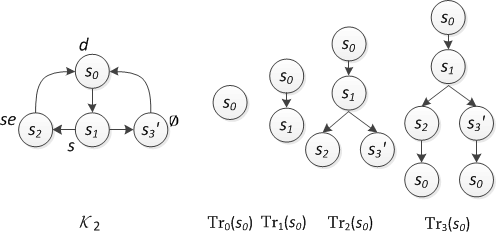
\includegraphics[width=10cm]{chapter05/NK2Tree1.png}
		\caption{初始结构$\mathcal{K}_2$(源于图\ref{Fig:chapter04:v1uv2})及其计算树示意图}\label{fig:K2Tree}
	\end{figure*}
	
	%\begin{figure*}[!htb]
	%	\centering
	%	% Requires \usepackage{graphicx}
	%	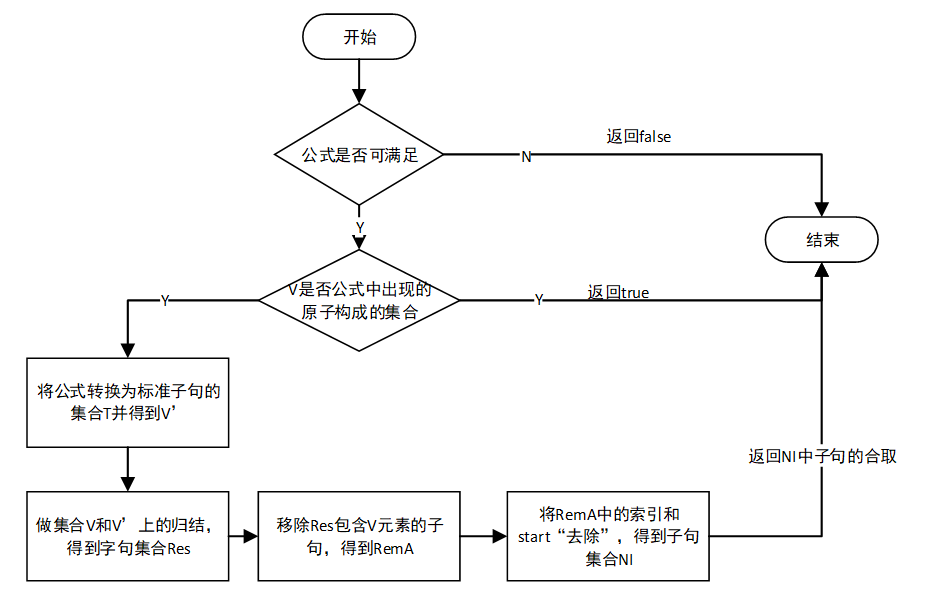
\includegraphics[width=15cm]{chapter04/frame.png}\\
	%	\caption{基于归结的遗忘的主要流程图}
	%	\label{Fig:chapter05:v1uv2}
	%\end{figure*}
	
\end{example}


下面的定理表示,特征公式描述了一个初始结构。此时,对系统结构的操作就可转换为对其特征公式的操作,如:下文中给定系统下的最弱充分条件计算。直观上,特征公式保持了给定初始结构在原子命题集$V$上的所有特性,即:具有$\overline{V}$-互模拟的两个初始结构关于$V$的特征公式逻辑等价。

\begin{theorem}\label{CF}
	令$V\subseteq \Ha$、$\Hm=(S,R,L,s_0)$且$\Hm'=(S',R', L',s_0')$,则:
	\begin{itemize}
		\item[(i)] $(\Hm',s_0') \models {\cal F}_V({\cal M},s_0)
		\text{ 当且仅当 }
		({\cal M},s_0) \lrto_{\overline V} ({\cal M}',s_0')$;
		
		\item[(ii)] 若$s_0 \lrto_{\overline V} s_0'$则${\cal F}_V(\Hm, s_0) \equiv {\cal F}_V(\Hm', s_0')$。
	\end{itemize}
	
\end{theorem}
\begin{proof}
	(i) 令${\cal F}_V(\Hm, s_0)$为$(\Hm, s_0)$关于$V$的特征公式。显然,$\IR({\cal F}_V(\Hm, s_0), \overline V)$。为了证明上述结论成立,首先证明$(\Hm, s_0) \models {\cal F}_V(\Hm, s_0)$。
	
	令$c={ch({\cal M},V)}$,由引理\ref{Bn:to:Tn}可知$(\Hm, s_0) \models {\cal F}_V(\Tr_c(s_0))$。下证特征公式里的另一部分,即:$(\Hm, s_0) \models \bigwedge_{s\in S} \ALL\GLOBAL\ G(\Hm, s)$,其中
	\[G(\Hm, s) = {\cal F}_V(\Tr_c(s)) \rto \left(\bigwedge_{(s,s_1) \in R} \EXIST \NEXT {\cal F}_V(\Tr_c(s_1))\right)\wedge \ALL \NEXT \left(\bigvee_{(s,s_1) \in R} {\cal F}_V(\Tr_c(s_1))\right).\]
	
	为此,下面证明$(\Hm, s_0) \models \ALL\GLOBAL\ G(\Hm, s)$。考虑下面两种情况:
	\begin{itemize}
		\item  若$(\Hm, s_0) \not \models {\cal F}_V(\Tr_c(s))$,显然$(\Hm, s_0) \models G(\Hm, s)$;
		\item 若$(\Hm, s_0) \models {\cal F}_V(\Tr_c(s))$:\\
		$(\Hm, s_0) \models {\cal F}_V(\Tr_c(s))$\\
		$\Rto$  $s_0 \lrto_{\overline V} s$ \hfill (引理\ref{div_s})
		
		$\forall (s, s_1)\in R$:\\
		$(\Hm, s_1) \models {\cal F}_V(\Tr_c(s_1))$  \hfill  ($s_1 \lrto_{\overline V} s_1$)\\
		$\Rto$ $(\Hm, s) \models \bigwedge_{(s,s_1)\in R}\EXIST \NEXT {\cal F}_V(\Tr_c(s_1))$\\
		$\Rto$ $(\Hm, s_0) \models$ $\bigwedge_{(s,s_1)\in R}\EXIST \NEXT {\cal F}_V(\Tr_c(s_1))$    \qquad  ($\IR(\bigwedge_{(s,s_1)\in R}\EXIST \NEXT {\cal F}_V(\Tr_c(s_1)), \overline V)$, $s_0 \lrto_{\overline V} s$)
		
		$\forall (s, s_1) \in R$:\\
		$(\Hm, s_1) \models \bigvee_{(s, s_2)\in R}{\cal F}_V(\Tr_c(s_2))$\\
		$\Rto$ $(\Hm, s) \models \ALL \NEXT \left( \bigvee_{(s, s_2)\in R} {\cal F}_V(\Tr_c(s_2)) \right)$ \\
		$\Rto$ $(\Hm, s_0) \models$  $\ALL \NEXT \left( \bigvee_{(s, s_2)\in R} {\cal F}_V(\Tr_c(s_2)) \right)$     ($\IR(\ALL \NEXT \left( \bigvee_{(s, s_2)\in R} {\cal F}_V(\Tr_c(s_2)) \right), \overline V)$, $s_0 \lrto_{\overline V} s$)\\
		$\Rto$ $(\Hm, s_0) \models G(\Hm, s)$。\\
		% where $s_i$ and $s_j$ are the successors of $s$.
	\end{itemize}
	
	对任意其它能从$s_0$可达的状态$s'$,都可以类似地证明$(\Hm,s')\models G(\Hm, s)$。
	因此,对任意$s\in S$,$(\Hm, s_0) \models \ALL\GLOBAL\ G(\Hm, s)$,从而$(\Hm, s_0) \models {\cal F}_V(\Hm, s_0)$。
	
	下面从两个方面证明(i)成立:
	
	$(\Lto)$ 证明:若$s_0 \lrto_{\overline V} s_0'$,则$(\Hm',s_0') \models {\cal F}_V(\Hm,s_0)$。因为$(\Hm, s_0) \models {\cal F}_V($ $\Hm, s_0)$且 $\IR({\cal F}_V$ $(\Hm, s_0), \overline V)$,由定理\ref{thm:V-bisimulation:EQ}可知
	$(\Hm',s_0') \models {\cal F}_V(\Hm,s_0)$。
	
	$(\Rto)$ 证明:若$(\Hm',s_0') \models {\cal F}_V(\Hm,s_0)$,则$s_0 \lrto_{\overline V} s_0'$。为此,下面证明对任意$n \geq 0$,$Tr_n(s_0) \lrto_{\overline V} Tr_n(s_0')$。
	
	
	\textbf{基始($n=0$):} 由特征公式的定义,显然$Tr_0(s_0) \equiv Tr_0(s_0')$成立。
	
	\textbf{归纳步骤($n>0$):} 假定对任意$k > 0$,都有$\Tr_k(s_0) \lrto_{\overline V} \Tr_k(s_0')$,下面证明$\Tr_{k+1}(s_0)$ $\lrto_{\overline V} \Tr_{k+1}(s_0')$。令$(s_0, s_1), (s_1, s_2)$, $\dots$, $(s_{k-1}, s_k) \in R$且$(s_0', s_1'), (s_1', s_2'), \dots, (s_{k-1}', s_k') \in R'$,即对于任意$0 \leq i \leq k-1$,$s_{i+1}$($s_{i+1}'$)是$s_i$($s_i'$)的直接后继状态。
	由归纳假设可知,只需证明$\Tr_1(s_k) \lrto_{\overline V} \Tr_1(s_k')$。
	
	(a) 由归纳假设可知$L(s_k) - \overline V = L'(s_k') - \overline V$。
	
	在讨论其它点时,首先考虑下面事实(\textbf{fact}):\\
	$(\Hm',s_0') \models {\cal F}_V(\Hm,s_0)$\\
	$\Rto$ $\forall s'\in S'$,$\forall s\in S$,\\ $(\Hm', s')\models {\cal F}_V(\Tr_c(s)) \rto$  $\left(\bigwedge_{(s,s_1)\in R} \EXIST \NEXT {\cal F}_V(\Tr_c(s_1))\right)\wedge \ALL \NEXT \left( \bigvee_{(s,s_1)\in R} {\cal F}_V(\Tr_c(s_1))\right)$  \\
	(I) $(\Hm', s_0') \models {\cal F}_V(\Tr_c(s_0)) \rto \left(\bigwedge_{(s_0, s_1) \in R} \EXIST \NEXT {\cal F}_V(\Tr_c(s_1))\right)$ $\wedge$ $\ALL \NEXT \left(\bigvee_{(s_0, s_1) \in R} {\cal F}_V(\Tr_c(s_1)) \right)$     \\
	(II) $(\Hm', s_0') \models {\cal F}_V(\Tr_c(s_0)))$  \hfill  (已知)\\
	(III) $(\Hm', s_0') \models \left(\bigwedge_{(s_0, s_1) \in R} \EXIST \NEXT {\cal F}_V(\Tr_c(s_1))\right)$ $\wedge$ $\ALL \NEXT \left(\bigvee_{(s_0, s_1) \in R} {\cal F}_V(\Tr_c(s_1)) \right)$  \hfill  ((I),(II))\\
	
	% It is apparent that $L'(s_0') - \overline V = L(s_0) - \overline V$;\\
	(b) 下证$\forall (s_k, s_{k+1}) \in R$,存在$(s_k', s_{k+1}') \in R'$,使得$L(s_{k+1}) - \overline V = L'(s_{k+1}') - \overline V$。\\
	(1) $(\Hm', s_0') \models \bigwedge_{(s_0, s_1) \in R} \EXIST \NEXT {\cal F}_V(\Tr_c(s_1))$  \hfill  (III)\\
	(2) $\forall (s_0, s_1) \in R$,$\exists (s_0', s_1') \in R'$,使得 $(\Hm', s_1') \models {\cal F}_V(\Tr_c(s_1))$  \hfill  (1)\\
	(3) $\Tr_c(s_1) \lrto_{\overline V} \Tr_c(s_1')$  \hfill  ((2), 引理\ref{Bn:to:Tn}) \\
	(4) $L(s_1) - \overline V = L'(s_1') - \overline V$  \hfill   ((3), $c \geq 0)$\\
	(5) $(\Hm', s_1') \models {\cal F}_V(\Tr_c(s_1)) \rto \left(\bigwedge_{(s_1,s_2)\in R} \EXIST \NEXT {\cal F}_V(\Tr_c(s_2))\right) \wedge \ALL \NEXT \left(\bigvee_{(s_1,s_2)\in R} {\cal F}_V(\Tr_c(s_2))\right)$     \hfill  \textbf{(fact)}\\
	(6) $(\Hm', s_1') \models \left(\bigwedge_{(s_1,s_2)\in R} \EXIST \NEXT {\cal F}_V(\Tr_c(s_2))\right) \wedge \ALL \NEXT \left(\bigvee_{(s_1,s_2)\in R} {\cal F}_V(\Tr_c(s_2))\right)$ \hfill ((2), (5))\\
	%(7) $\dots \dots$ \\
	(7) $(\Hm', s_k') \models \left(\bigwedge_{(s_k,s_{k+1})\in R} \EXIST \NEXT {\cal F}_V(\Tr_c(s_{k+1}))\right) \wedge \ALL \NEXT \left(\bigvee_{(s_k,s_{k+1})\in R} {\cal F}_V(\Tr_c(s_{k+1}))\right)$       \hfill (与(6)类似)\\
	(8) $\forall (s_k, s_{k+1}) \in R$,$\exists (s_k', s_{k+1}') \in R'$,使得$(\Hm', s_{k+1}') \models {\cal F}_V(\Tr_c(s_{k+1}))$  \hfill  (7)\\
	(9) $\Tr_c(s_{k+1}) \lrto_{\overline V} \Tr_c(s_{k+1}')$    \hfill ((8), 引理\ref{Bn:to:Tn}) \\
	(10) $L(s_{k+1}) - \overline V = L'(s_{k+1}') - \overline V$  \hfill   ((9), $c \geq 0)$\\
	
	(c) 下证$\forall (s_k', s_{k+1}') \in R'$,存在$(s_k, s_{k+1})\in R$,使得$L(s_{k+1}) - \overline V = L'(s_{k+1}') - \overline V$。\\
	(1) $(\Hm', s_k') \models \ALL \NEXT \left(\bigvee_{(s_k,s_{k+1})\in R} {\cal F}_V(\Tr_c(s_{k+1}))\right)$  \hfill (上面的(7))\\
	(2) $\forall (s_k', s_{k+1}') \in R'$,$\exists (s_k, s_{k+1}) \in R$,使得$(\Hm', s_{k+1}') \models {\cal F}_V(\Tr_c(s_{k+1}'))$  \hfill (1) \\
	(3) $\Tr_c(s_{k+1}) \lrto_{\overline V} \Tr_c(s_{k+1}')$    \hfill ((2), 引理\ref{Bn:to:Tn}) \\
	(4) $L(s_{k+1}) - \overline V = L'(s_{k+1}') - \overline V$  \hfill   ((3), $c \geq 0)$\\
	
	(ii) 由引理\ref{lem:Vb:TrFormula:Equ}和\ref{div_s}易得。
	
\end{proof}

上文描述了初始结构特征公式的计算,下面给出例\ref{exam:SNCandWSC}的详细计算过程。
\begin{example}[例~\ref{exam:SNCandWSC}的延续]
	%\label{exam:SNCandWSC}
	令$\Ha=\{d,se,sp,s\}$和$V=\{d,se\}$,求$s$在$V$和初始结构${\cal K} = (\Hm,s_0)$上的WSC,其中$\Hm$为例~\ref{car_manufacturing}中初始状态为$s_0$的汽车制造企业模型结构。
	
	由定理~\ref{thm:inK:SNC}可知,$s$在$V$和初始结构${\cal K} = (\Hm,s_0)$上的WSC为$\neg \CTLforget({\cal F}_{\Ha}({\cal K}) \wedge \neg s, \{s\} \cup \{sp\})$。
	\begin{align*}
		&	\CTLforget({\cal F}_{\Ha}({\cal K}) \wedge \neg s, \{s\} \cup \{sp\})\\
		&	\equiv \CTLforget(\CTLforget({\cal F}_{\Ha}({\cal K}) \wedge \neg s, \{sp\}), \{s\})\\
		&	\equiv \CTLforget(\CTLforget({\cal F}_{\Ha}({\cal K}), \{sp\})\wedge \neg s, \{s\}).
	\end{align*}
	
	${\cal K}_1 \models \CTLforget({\cal F}_{\Ha}({\cal K}), \{sp\})$\\
	$\LRto$ 存在${\cal K}_1' \lrto_{\{sp\}} {\cal K}_1$,使得${\cal K}_1' \models {\cal F}_{\Ha}({\cal K})$和\\
	$\LRto$ 存在${\cal K}_1' \lrto_{\{sp\}} {\cal K}_1$,使得${\cal K}_1' \lrto_{\emptyset} {\cal K}$\\
	$\LRto$ 存在${\cal K}_1' \lrto_{\{sp\}} {\cal K}$和${\cal K}_1' \models {\cal F}_{V\cup \{s\}}({\cal K})$ \hfill (定理~\ref{CF})\\
	$\LRto$ ${\cal K}_1 \models {\cal F}_{V\cup \{s\}}({\cal K})$。
	
	由此可知,$ \CTLforget({\cal F}_{\Ha}({\cal K}), \{sp\}) \equiv {\cal F}_{V\cup \{s\}}({\cal K})$。所以要计算$\neg \CTLforget({\cal F}_{\Ha}({\cal K}) \wedge \neg s, \{s\}$ $\cup \{sp\})$,只需计算$\neg \CTLforget({\cal F}_{V\cup \{s\}}({\cal K})\wedge \neg s, \{s\})$。令$V' = V \cup \{s\} = \{d,se,s\}$,则$\overline{V'} = \{sp\}$。
	
	
	易知,除了$s_2$和$s_4$是$\overline{V'}$-互模拟的以外,其余都是$V'$-可区分的,且$\dis_{V'}(\Hm, s_i, s_j, 0)$,其中$i\not =j$且$i$和$j$不能同时分别取值2和4。
	因此,可以计算$\Hm$关于$V'$的特征数为:
	$$ch(\Hm, V')=\max\{k\mid s,s'\in S \text{ 且 } \dis_{V'}({\cal M},s,s',k)\} = 0\hbox{。}$$
	
	
	所以,可以由以下步骤计算${\cal K}_2$关于$V$的特征公式:
	\begin{align*}
		{\cal F}_{V'}(\Tr_0(s_0)) &= d \wedge \neg se \wedge \neg s, \qquad \qquad \qquad \qquad \quad {\cal F}_{V'}(\Tr_0(s_1)) = \neg d \wedge \neg se \wedge s, \\
		{\cal F}_{V'} (\Tr_0(s_2)) &= {\cal F}_{V'} (\Tr_0(s_4)) = \neg d \wedge se \wedge \neg s,  \qquad  {\cal F}_{V'}(\Tr_0(s_3) = \neg d \wedge \neg se\wedge \neg s,\\
		{\cal F}_{V'}(\Hm, s_0)& \equiv d \wedge \neg se \wedge \neg s \wedge \\
		& \ALL \GLOBAL(d \wedge \neg se \wedge \neg s \rto \ALL\NEXT(\neg d \wedge \neg se \wedge s))\wedge \\
		& \ALL \GLOBAL(\neg d \wedge \neg se \wedge s \rto [\ALL\NEXT((\neg d \wedge se \wedge \neg s) \vee (\neg d \wedge \neg se\wedge \neg s)) \wedge\\ &\EXIST\NEXT(\neg d \wedge se \wedge \neg s) \wedge \EXIST\NEXT (\neg d \wedge \neg se\wedge \neg s)]) \wedge\\
		& \ALL \GLOBAL(\neg d \wedge \neg se\wedge \neg s \rto \ALL\NEXT(d \wedge \neg se \wedge \neg s)) \wedge\\
		& \ALL \GLOBAL(\neg d \wedge se \wedge \neg s \rto \ALL\NEXT(d \wedge \neg se \wedge \neg s)).
	\end{align*}
	令:
	\begin{align*}
		\varphi_1&  = d \wedge \neg se \wedge \neg s \rto \ALL\NEXT(\neg d \wedge \neg se \wedge s)\equiv \neg d \vee se \vee s \vee \ALL\NEXT(\neg d \wedge \neg se \wedge s),\\
		\varphi_2& = \neg d \wedge \neg se \wedge s \rto \ALL\NEXT(\neg d \wedge se \wedge \neg s) \equiv d \vee  se \vee \neg s \vee\\
		& [\ALL\NEXT((\neg d \wedge se \wedge \neg s) \vee (\neg d \wedge \neg se\wedge \neg s)) \wedge\EXIST\NEXT(\neg d \wedge se \wedge \neg s) \wedge \EXIST\NEXT (\neg d \wedge \neg se\wedge \neg s)],\\
		\varphi_3 &=\neg d \wedge \neg se\wedge \neg s \rto \ALL\NEXT(d \wedge \neg se \wedge \neg s)\equiv d \vee se \vee s \vee \ALL\NEXT(d \wedge \neg se \wedge \neg s),\\
		\varphi_4 &= \neg d \wedge se \wedge \neg s \rto \ALL\NEXT(d \wedge \neg se \wedge \neg s)\equiv d \vee \neg se \vee s \vee \ALL\NEXT(d \wedge \neg se \wedge \neg s).
	\end{align*}
	此外,令
	\begin{align*}
		& \psi_1 = \neg d \vee se \vee s && \psi_2 = d \vee  se \vee \neg s \\
		& \psi_3 = d \vee se \vee s && \psi_4 = d \vee \neg se \vee s\\
		& \alpha_1 = \ALL\NEXT(\neg d \wedge \neg se \wedge s) && \alpha_2 = \ALL\NEXT((\neg d \wedge se \wedge \neg s) \vee (\neg d \wedge \neg se\wedge \neg s))\\
		& \alpha_3 = \EXIST\NEXT(\neg d \wedge se \wedge \neg s) \wedge \EXIST\NEXT (\neg d \wedge \neg se\wedge \neg s) && \alpha_4 = \ALL\NEXT(d \wedge \neg se \wedge \neg s)\\
		& \alpha_5 = \ALL\NEXT(d \wedge \neg se \wedge \neg s) && \psi = d \wedge \neg se \wedge \neg s.
	\end{align*}
	则,
	\begin{align*}
		& \psi \wedge \varphi_1 \wedge \varphi_2 \wedge \varphi_3\wedge \varphi_4 
		\equiv (\psi \wedge \psi_1 \wedge \psi_2 \wedge \psi_3 \wedge \psi_4) \vee (\psi \wedge \psi_1 \wedge \psi_2 \wedge \psi_3 \wedge \alpha_5) \vee\\
		& (\psi \wedge \psi_1 \wedge \psi_2 \wedge \alpha_4 \wedge \psi_4) \vee (\psi \wedge \psi_1 \wedge \psi_2 \wedge \alpha_4 \wedge \alpha_5) \vee\\
		& (\psi \wedge \psi_1 \wedge \alpha_2 \wedge \alpha_3 \wedge \psi_3 \wedge \psi_4) \vee (\psi \wedge \psi_1 \wedge \alpha_2 \wedge \alpha_3 \wedge \psi_3 \wedge \alpha_4) \vee \\
		& (\psi \wedge \psi_1 \wedge \alpha_2 \wedge \alpha_3 \wedge \alpha_4 \wedge \psi_4) \vee (\psi \wedge \psi_1 \wedge \alpha_2 \wedge \alpha_3 \wedge \alpha_4 \wedge \alpha_5) \vee\\
		& (\psi \wedge \alpha_1 \wedge \psi_2 \wedge \psi_3 \wedge \psi_4) \vee (\psi \wedge \alpha_1 \wedge \psi_2 \wedge \psi_3 \wedge \alpha_5)\vee\\
		& (\psi \wedge \alpha_1 \wedge \psi_2 \wedge \alpha_4 \wedge \psi_4) \vee (\psi \wedge \alpha_1 \wedge \psi_2 \wedge \alpha_4 \wedge\alpha_5)\vee \\
		& (\psi \wedge \alpha_1 \wedge \alpha_2 \wedge \alpha_3 \wedge \psi_3 \wedge \psi_4) \vee (\psi \wedge \alpha_1 \wedge \alpha_2 \wedge \alpha_3\wedge \psi_3 \wedge \alpha_5) \vee \\
		& (\psi \wedge \alpha_1 \wedge \alpha_2 \wedge \alpha_3 \wedge \alpha_4 \wedge \psi_4) \vee (\psi \wedge \alpha_1 \wedge \alpha_2 \wedge \alpha_3 \wedge \alpha_4 \wedge \alpha_5).\\
		\\
		%\end{align*}
		%\begin{align*}
		& \varphi_1 \wedge \varphi_2 \wedge \varphi_3\wedge \varphi_4 
		\equiv (\psi_1 \wedge \psi_2 \wedge \psi_3 \wedge \psi_4) \vee (\psi_1 \wedge \psi_2 \wedge \psi_3 \wedge \alpha_5) \vee\\
		& (\psi_1 \wedge \psi_2 \wedge \alpha_4 \wedge \psi_4) \vee (\psi_1 \wedge \psi_2 \wedge \alpha_4 \wedge \alpha_5) \vee\\
		& (\psi_1 \wedge \alpha_2 \wedge \alpha_3 \wedge \psi_3 \wedge \psi_4) \vee ( \psi_1 \wedge \alpha_2 \wedge \alpha_3 \wedge \psi_3 \wedge \alpha_4) \vee \\
		& ( \psi_1 \wedge \alpha_2 \wedge \alpha_3 \wedge \alpha_4 \wedge \psi_4) \vee ( \psi_1 \wedge \alpha_2 \wedge \alpha_3 \wedge \alpha_4 \wedge \alpha_5) \vee\\
		& (\alpha_1 \wedge \psi_2 \wedge \psi_3 \wedge \psi_4) \vee ( \alpha_1 \wedge \psi_2 \wedge \psi_3 \wedge \alpha_5)\vee\\
		& (\alpha_1 \wedge \psi_2 \wedge \alpha_4 \wedge \psi_4) \vee ( \alpha_1 \wedge \psi_2 \wedge \alpha_4 \wedge\alpha_5)\vee \\
		& (\alpha_1 \wedge \alpha_2 \wedge \alpha_3 \wedge \psi_3 \wedge \psi_4) \vee (\alpha_1 \wedge \alpha_2 \wedge \alpha_3\wedge \psi_3 \wedge \alpha_5) \vee \\
		& ( \alpha_1 \wedge \alpha_2 \wedge \alpha_3 \wedge \alpha_4 \wedge \psi_4) \vee ( \alpha_1 \wedge \alpha_2 \wedge \alpha_3 \wedge \alpha_4 \wedge \alpha_5).
	\end{align*}
	所以,
	\begin{align*}
		&\neg \CTLforget({\cal F}_{V\cup \{s\}}({\cal K})\wedge \neg s, \{s\}) \\
		& \equiv \neg \CTLforget({\cal F}_{V\cup \{s\}}({\cal K}), \{s\})\\
		& \equiv \neg \CTLforget(\psi \wedge \ALL \GLOBAL(\varphi_1 \wedge \varphi_2 \wedge \varphi_3\wedge \varphi_4),\{s\})\\	
		& \equiv \neg(\CTLforget(\psi \wedge \varphi_1 \wedge \varphi_2 \wedge \varphi_3\wedge \varphi_4, \{s\}) \wedge \ALL \GLOBAL \CTLforget(\varphi_1 \wedge \varphi_2 \wedge \varphi_3\wedge \varphi_4, \{s\}))\\
		& \equiv  \neg \bigg(\Big(d \vee \big((d\vee se) \wedge \ALL\NEXT(d \wedge \neg se)\big) \vee \big((d \vee se \vee \ALL\NEXT \neg d) \wedge \EXIST\NEXT(\neg d \wedge se) \wedge \EXIST\NEXT(\neg d \wedge \neg se)\big) \\
		& \vee (d \wedge \ALL\NEXT(\neg d \wedge \neg se)) \vee \big((d\vee \neg se) \wedge \EXIST\NEXT\neg d\big) \Big) \wedge\\
		& \ALL \GLOBAL\Big(\big((d \vee se) \wedge \ALL\NEXT(d \wedge \neg se)\big) \vee \big(\ALL\NEXT \neg d \wedge \EXIST\NEXT(\neg d \wedge se) \wedge\\
		& \EXIST\NEXT(\neg d \wedge \neg se)\big) \vee \big((d\vee se) \wedge \ALL\NEXT(\neg d \wedge \neg se)\big) \vee \EXIST\NEXT \neg d\Big)
		\bigg)\hbox{。}
	\end{align*}
\end{example}

\subsection{遗忘封闭性及复杂性}\label{chapter06:sec:close}
当$\CTL$公式的长度(符号的个数)为$n$时,由小模型理论可知,定义在状态个数为$k=n8^n$的状态空间${\cal S}=\{s_1,s_2,\dots, s_k\}$上的初始Kripke结构能保证公式的可满足性~\cite{DBLP:journals/jcss/EmersonH85}。
对于其它拥有同样大小状态空间上的任意初始结构,都能在状态空间${\cal S}$上找到一个初始结构与之互模拟,且由定理\ref{CF}可知它们有相同的特征公式。
因此,只有有限个初始结构作为该公式的候选模型。从而下面结论成立。
%这一事实可以用下面引理表示。

\begin{lemma}\label{lem:models:formula}
	给定$\CTL$公式$\varphi$,下面等式成立:
	\begin{equation*}
		\varphi\equiv \bigvee_{(\Hm, s_0)\in\Mod(\varphi)}{\cal F}_{\cal A}(\Hm, s_0).
	\end{equation*}
\end{lemma}
\begin{proof}
	令$(\Hm', s_0')$为$\varphi$的模型。由定理\ref{CF}可知$(\Hm', s_0') \models {\cal F}_{\Ha}(\Hm', s_0')$,则:
	$$(\Hm', s_0') \models \bigvee_{(\Hm, s_0)\in \Mod(\varphi)} {\cal F}_{\Ha}(\Hm, s_0).$$
	
	另一方面,假定$(\Hm', s_0')$为$\bigvee_{(\Hm, s_0)\in \Mod(\varphi)} {\cal F}_{\Ha}(\Hm, s_0)$的模型。则存在$(\Hm, s_0)\in \Mod(\varphi)$ ,使得 $(\Hm', s_0') \models {\cal F}_{\Ha}(\Hm,$ $s_0)$。由定理\ref{CF}可知$(\Hm, s_0) \lrto_{\emptyset} (\Hm', s_0')$,从而由定理\ref{thm:V-bisimulation:EQ}可知$(\Hm, s_0)$是 $\varphi$的一个模型。
\end{proof}

该结论表明:任意$\CTL$公式都与其模型的特征公式的析取逻辑等价。这对遗忘理论的封闭性提供了重要的理论支撑,即:从公式里遗忘原子命题集$V$中的元素只需找到与给定公式的模型$V$-互模拟的那些模型就能确定遗忘的结果。形式化地,对于给定的公式$\varphi$和原子命题集$V$,从$\varphi$中遗忘$V$中的元素得到的结果为:
\begin{equation*}
	\bigvee_{{\cal K}\in  \{{\cal K}'\mid \exists {\cal K}''\in\Mod(\phi),\ {\cal K}''\lrto_V{\cal K}'\}} {\cal F}_{\overline V}({\cal K}).
\end{equation*}



下面分析遗忘在$\CTL$段$\CTL_{\ALL\FUTURE}$下推理问题的复杂性结果,其中$\CTL_{\ALL\FUTURE}$表示$\CTL$公式只包含时序算子$\ALL \FUTURE$的子类。
这一类公式在并发系统中的互斥和等待等属性描述中有重要作用~\cite{Baier:PMC:2008}。尽管这类公式是相对简单的,但是下面将要说明判定一个模型是否为此类公式遗忘结果的模型是$\textsc{NP}$-完全的。
\begin{proposition}[模型检测]
	\label{modelChecking}
	给定一个结构 $(\Hm,s_0)$、原子命题集$V\subseteq{\cal A}$和公式 $\varphi \in \CTL_{\ALL\FUTURE}$,判定 $(\Hm,s_0)$ 是否为$\CTLforget(\varphi, V)$的模型是 \textsc{NP}-完全的。
\end{proposition}
\begin{proof}
	在$\textsc{NP}$中. 假定$(\Hm,s_0) \models \CTLforget(\varphi,V)$,则存在一个初始结构$(\Hm', s_0')$,使得\ (a) $(\Hm',s_0') \models \varphi$且\ (b) $(\Hm,s_0) \lrto_V (\Hm',s_0')$。已有结果表明:(a)能在$\Hm'$和 $\varphi$的大小的多项式时间内完成~\cite{DBLP:books/daglib/0007403};条件(b)也可用Baier等人的推论 7.45~\cite{Baier:PMC:2008}的方法证明能在多项式时间内完成。
	又因为猜$(\Hm,s_0)$多项式大小的初始结构$(\Hm',s_0')$能在多项式时间内完成。因此,这一问题在$\textsc{NP}$中。
	
	$\textsc{NP}$-难. 已经证明命题逻辑下遗忘的模型检测是$\textsc{NP}$-难的,由于命题逻辑下的遗忘是$\CTL$的一种~\cite{Zhang2008Properties}。因此,上述问题是$\textsc{NP}$-难的。
\end{proof}

%关于遗忘的逻辑蕴涵问题也是值得考虑的。
下面讨论$\CTL_{\ALL\FUTURE}$段下关于遗忘的逻辑蕴涵问题的复杂性。
下文用记号$\alpha \models^? \beta$表示“$\alpha$是否逻辑蕴涵$\beta$”。

\begin{theorem}[Entailment]
	\label{thm:comF}
	令 $\varphi$和 $\psi$为$\CTL_{\ALL \FUTURE}$中的两个公式, $V$为原子命题集。则:
	\begin{itemize}
		\item[(i)] 判定  $\CTLforget(\varphi, V ) \models^? \psi$是 co-$\textsc{NP}$-完全的,
		\item[(ii)] 判定  $\psi \models^? \CTLforget(\varphi, V)$是 $\Pi_2^{\textsc{P}}$-完全的,
		\item[(iii)] 判定 $\CTLforget(\varphi, V) \models^? \CTLforget(\psi, V)$是 $\Pi_2^{\textsc{P}}$-完全的。
	\end{itemize}
\end{theorem}
\begin{proof}
	(i) co-$\textsc{NP}$-难. 已有结论表明,判定公式$\varphi$是否是可满足的是$\textsc{NP}$-完全的~\cite{meier2009complexity}。令$\psi \equiv \bot$,只需证明$\varphi$是不可满足的,该问题是co-$\textsc{NP}$-难的。所以,原问题是co-$\textsc{NP}$-难的。
	
	在co-$\textsc{NP}$中. 定理\ref{thm:exist}表明$\CTLforget(\varphi, V) \models \psi$当且仅当 $\varphi \models \psi$且 $\IR(\psi, V)$。
	在$\CTL_{\ALL \FUTURE}$中,判定 $\varphi \models \psi$是co-$\textsc{NP}$的~\cite{meier2009complexity}。
	这里证明 $\IR(\psi, V)$是否成立是 co-$\textsc{NP}$的。不失一般性地,假定$\psi$是可满足的,则 $\psi$有一个大小为$|\psi|$的多项式的模型。
	这里讨论该问题的补问题:判定 $\psi$是$V$-有关的,即 $\neg \IR(\psi, V)$。显然,$\neg \IR(\psi, V)$当且仅当存在$\psi$的一个模型 $(\Hm,s_0)$和大小为$|\psi|$的多项式的初始结构 $(\Hm',s_0')$,使得 $(\Hm,s_0) \lrto_V (\Hm',s_0')$且 $(\Hm',s_0') \not \models \psi$。因此,判定$\neg \IR(\psi, V)$是否成立有如下两个步骤:(1)猜两个大小为$|\psi|$的多项式的初始结构$(\Hm,s_0)$和 $(\Hm',s_0')$,使得 $(\Hm,s_0) \models \psi$且 $(\Hm',s_0') \not \models \psi$;(2)检查 $(\Hm,s_0) \lrto_V (\Hm',s_0')$。
	显然, (1)和(2)都是能在多项式时间内完成的。
	
	(ii) 在$\Pi_2^{\textsc{P}}$中. 考虑这一问题的补问题。猜一个大小为$|\psi|$的多项式的$\psi$的 模型 $(\Hm,s_0)$且检查 是否 $(\Hm, s_0) \not \models \CTLforget(\varphi, V)$。
	由命题\ref{modelChecking} 可知这一问题在 $\Sigma_2^{\textsc{P}}$中。因此,原问题在$\Pi_2^{\textsc{P}}$中。
	
	$\Pi_2^{\textsc{P}}$-难. 令$\psi \equiv \top$。 则这一问题被归约为判定$\CTLforget(\varphi, V)$的有效性问题。 
	由于命题遗忘是$\CTL$遗忘的特殊情形,因此该问题的困难属性直接来源于文献\cite{DBLP:journals/jair/LangLM03}。
	
	(iii) 在$\Pi_2^{\textsc{P}}$中. 假定 $\CTLforget(\varphi, V) \not \models \CTLforget(\psi, V)$。则存在一个初始结构 $(\Hm,s) 
	\models \CTLforget(\varphi, V)$ 且$(\Hm,s) \not \models \CTLforget(\psi, V)$,即存在一个初始结构$(\Hm_1,s_1) \lrto_V (\Hm,s)$,使得 $(\Hm_1, s_1) \models \varphi$ 但是对任意$(\Hm, s) \lrto_V (\Hm_2,s_2)$,$(\Hm_2, s_2) \not \models \psi$。
	由命题\ref{modelChecking}的证明可知,$(\Hm,s)$和 $(\Hm_1,s_1)$ 能在$|\varphi|$、$|\psi|$和$|V|$的多项式时间内完成。 
	显然,猜使得$(\Hm_1,s_1) \lrto_V (\Hm,s)$ 成立的大小为$|\varphi|$多项式的 $(\Hm,s)$和 $(\Hm_1,s_1)$ 可以在多项式时间内完成,且 对任意 $(\Hm, s) \lrto_V (\Hm_2,s_2)$,检查 $(\Hm_2,s_2) \not \models \psi$可以在 $|\psi|$和 $|\Hm_2|$的多项式时间内完成。
	因此,该问题是 $\Pi_2^{\textsc{P}}$的。
	
	$\Pi_2^{\textsc{P}}$-难. 由于 $\IR(\CTLforget(\psi, V), V)$,因此 $\CTLforget(\varphi, V) \models \CTLforget(\psi, V)$当且仅当 $\varphi \models \CTLforget(\psi,$ $V)$。 所以由(ii)不难证明该问题。
\end{proof}



定理\ref{thm:comF}蕴涵下列结论。
\begin{corollary}
	令 $\varphi$和 $\psi$为 $\CTL_{\ALL \FUTURE}$中的两个公式,$V$原子公式集。则
	\begin{itemize}
		\item[(i)] 判定 $\psi \equiv^?\CTLforget(\varphi, V)$是 $\Pi_2^{\textsc{P}}$-完全的,
		\item[(ii)] 判定 $\CTLforget(\varphi, V) \equiv^? \varphi$是 co-$\textsc{NP}$-完全的,
		\item[(iii)] 判定 $\CTLforget(\varphi, V) \equiv^? \CTLforget(\psi, V)$是$\Pi_2^{\textsc{P}}$-完全的。
	\end{itemize}
\end{corollary}


\subsection{基于模型的遗忘算法}\label{chapter06:sec:algm}
这里提出基于模型的遗忘算法,该算法与第\ref{cha4:sec:alg}节中基于语法的算法不同。本小节的算法通过计算所有可能的模型来计算遗忘,且其正确性可由引理\ref{lem:models:formula}和定理\ref{CF}保证。


\begin{algorithm}[tb]
	\caption{\small 基于模型的$\CTL$遗忘过程}%A Model-based \CTL\ Forgetting Procedure}
	\label{alg:compute:forgetting:by:VB}
	\LinesNumbered
	\KwIn{$\CTL$公式$\varphi$和原子命题集$V$}%A \CTL formula $\varphi$ and a set $V$ of atoms}
	\KwOut{$\CTLforget(\varphi, V)$}% ????
	$\psi \lto \bot$\;
	\ForEach{$\cal A$ 和$\cal S$上的初始结构$\cal K$}{
	%\ForEach{initial \MPK-structure $\cal K$ (over $\cal A$ and $\cal S$)}{
		\lIf{${\cal K}\not\models\varphi$}{{\bf continue}} \\
		\ForEach{满足${\cal K}\lrto_{ V}{\cal K}'$的初始结构${\cal K}'$}{
			$\psi \lto \psi \lor {\cal F}_{\overline V}({\cal K}')$\;
		}
	}
	\Return $\psi$\;
\end{algorithm}




这里给出如何计算从规范中遗忘一些原子命题。 
\begin{example}\label{ex:6}
	对于图\ref{BVM}中的 ${\cal K}_1$,假定一个已知的规范(性质)为$\alpha = \EXIST\FUTURE(se \wedge sp)$。显然 ${\cal K}_1$满足 $\alpha$。若想移除 $sp$,即从 $\alpha$中遗忘 $sp$,则 $\CTLforget(\alpha,\{ sp\}) \equiv \EXIST\FUTURE se$。此时,该汽车制造公司可以用新的规范$\EXIST\FUTURE se$(这保证驾车最终会被生产)引导未来汽车的生产。
\end{example}


如下所述,通过计算所有可能的模型是非常低效的。但是,这为从理论的角度探索遗忘有重要作用。


\begin{proposition}\label{pro:time:alg1}
	令 $\varphi$为$\CTL$公式,$V\subseteq \Ha$为原子命题集,状态空间大小为 $|{\cal S}|=m$, $|\Ha|=n$,$|V|=x$。使用算法\ref{alg:compute:forgetting:by:VB}计算从$\varphi$中遗忘$V$中原子的空间复杂度为 $O((n-x)m^{2(m+2)}2^{nm}  \log m)$,且时间复杂性至少与空间复杂性相同。
\end{proposition}
\begin{proof}
	假定每个状态或原子命题占据$\log m$的空间且$n\leq m$,则一个状态对$(s,s')$占据$2\times \log m$位(bit)。对任意$B \subseteq {\cal S}$和$s_0\in B$,构造如下初始结构$(\Hm,s_0)$,其中$\Hm = (B,R,L,s_0)$,则$R$中至多有$\frac{|B|^2}{2}$个状态对且$L$中至多$|B|\times n$个$(s,A)$对($A\subseteq \Ha$)。因此,$(\Hm,s_0)$至多占据$(|B|+|B|^2+|B|\times n)\times \log m$位。此外,对于状态集$B$,初始状态有$|B|$种选择,有$|B|^{|B|}$种关系$R$,$(2^n)^{|B|}$种标签函数$L$。
	
	在最坏的情形下(即$|B|=m$),可构成$m \times  (m^m \times  2^{nm} \times  m)$个初始结构。因此,最多有$m^{m+2} \times  2^{nm}$个初始结构,且最多花费$(m^{m+2} \times  2^{nm} \times  (m + m^2 + nm))\times  \log m$位。
	
	令 $k = n-x$,对任意有$i\geq 1$个状态的初始结构${\cal K} = (\Hm,s_0)$,其中$\Hm = (B,R,L,s_0)$。
	在最坏的情形下(即$ch(\Hm,V) = i$时),需要$N(i) = P_i(s_0) + i \times  (P_i(s) + i \times P_i(s'))$位来存储${\cal K}$在$\overline{V}$上的特征公式。
	其中$s',s\in B$,$P_i(y)$是存储${\cal F}_{\overline{V}}(\Tr_i(y))$($y\in B$)所用的空间(这里假定$\EXIST\NEXT$和$\ALL\NEXT$使用了相同的存储单位)。
	
	${\cal F}_{\overline{V}}(\Tr_i(y))$($0\leq n \leq i$)被递归地定义如下:
	\begin{align*}
		&(1) n=0,  \qquad P_0(y) = k\\
		&(2) n=1, \qquad  P_1(y) = k + i\times k = k + i\times P_0(y)\\
		&(3) n=2, \qquad P_2(y) = k + i\times (k + i\times k) = k+i\times P_1(y)\\
		& \dots \qquad \qquad \dots\\
		&(i+1) n = i, \quad P_i(y) = k + i \times  P_{i-1}(y).
	\end{align*}
	
	因此,有
	\begin{align*}
		P_i(y) & = k + i\times k + i^2 \times  k + \dots + i^i \times  k = \frac{i^i -1}{i-1} k,\\
		N(i) & = P_i(s_0) + i\times  (P_i(s) + i \times  P_i(s'))\\
		& = (i^2 + i +1) P_i(y) \\
		& = (i^2 + i+1)\frac{i^i -1}{i-1} k.
	\end{align*}
	
	在最坏的情形下(即具有$m$个状态的初始结构)有$m^{m+2} \times  2^{nm}$个初始结构,需要$(m^{m+2} \times  2^{nm} \times  N(m)) \times  \log m$位来存储遗忘的结果。
	
	因此,空间复杂性为$O((n-x)m^{2(m+2)}2^{nm}\times  \log m)$。
\end{proof}



\section{基于归结的遗忘计算方法}
\label{chapter05:sec:resolution}
	已有结果显示,任意$\CTL$公式可以转换为$\CTLsnf$子句集。归结是一种以子句为计算对象的判断可满足性的方法。本节提出一种基于归结的计算遗忘的方法,
	其主要思想是:首先,将给定的$\CTL$公式转换为$\CTLsnf$子句集(这一部分在第\ref{chapter02}章已经给出了详细的介绍;其次,在相应的原子命题集$V$上使用归结规则得到归结结果;最后,“消除”之前引入的索引和$\start$,最终得到遗忘的结果。其主要流程图如图\ref{Fig:chapter05:v1uv2}所示。
	$\CTL$遗忘结果不总是存在的,因此,基于归结的方法在有的情况下不能计算出遗忘结果。然而,在有些$\CTL$子类下,本章提出的方法能够计算出其遗忘结果。
\begin{figure*}[!htb]
	\centering
	% Requires \usepackage{graphicx}
	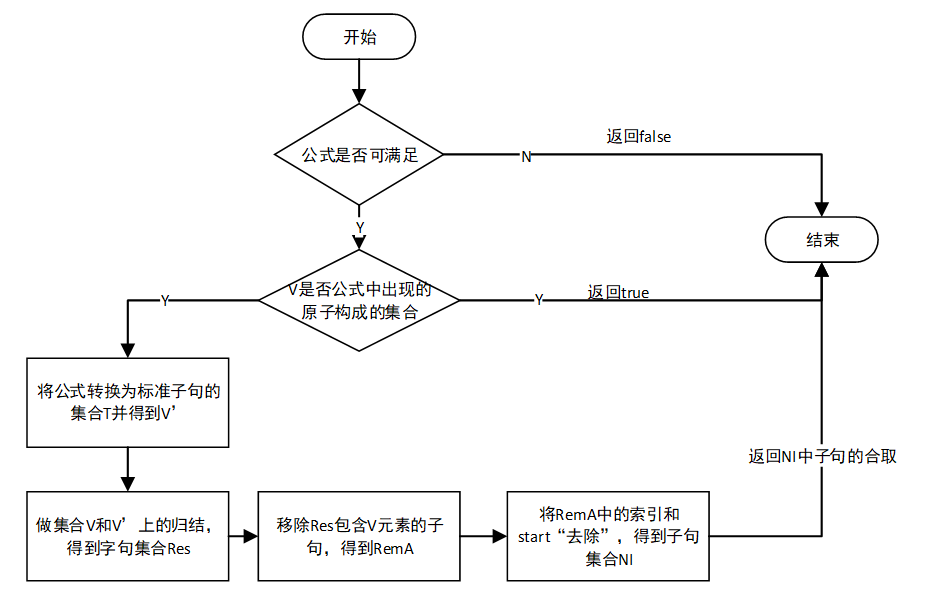
\includegraphics[width=15cm]{chapter04/frame.png}\\
	\caption{基于归结的遗忘的主要流程图}
	\label{Fig:chapter05:v1uv2}
\end{figure*}

%虽然在第\ref{chapter02}章详细介绍了命题逻辑和模态逻辑S5下基于归结的计算遗忘的方法,但值得注意的是$\CTL$公式没有像这两种逻辑一样有标准的自身语言子句形式,而$\CTL$的子句是有索引的。这就注定了$\CTL$下基于归结的遗忘与上述两者的不同,而且也应该要复杂一些(虽有不同,但也可以借鉴)。
本章展示如何使用表\ref{tab:res}中的归结规则来计算$\CTL$遗忘。
为了计算从$\CTL$公式$\varphi$中遗忘集合$V$中的原子命题,
%为了实现这一目标,
需要解决如下两个主要问题:
\begin{itemize}
	\item[(1)] 如何表示$\CTL$公式和带索引的$\CTL$公式之间的关系?如在第\ref{chapter02}章中所说,将一个$\CTL$公式转换为$\CTLsnf$子句集会引入新的原子命题和索引。虽然已有的研究说明,$\CTL$公式可以转换为带索引的公式集并保证其可满足性,然而并没有表明这两种形式的公式之间的模型具有怎样的联系。
	本章从互模拟等价的角度探讨$\CTL$公式和归结等过程得到的(带索引)公式之间的联系,为计算遗忘提供理论基础。
	%本章给出一种扩展的互模拟定义,以描述两种公式的模型之间的关系。
	\item[(2)] 如何“移除”无关的原子命题(包括需要遗忘的原子命题和转换过程中引入的新的原子命题),以及如何“消除”索引?为此,本章给出“移除”原子命题的一般操作,并提出一种一般化的Ackermann引理。为了“消除”索引,探索几个逻辑等价关系。%,详见第\ref{cha4:sec:resf}节。
	%对应算法\ref{alg:compute:forgetting:by:Resolution}中的$\emph{Removing\_index}(\emph{RemA})$过程。
\end{itemize}

%此外,详细描述基于Prolog上述算法的实现并分析实验结果。

本章其余部分组织如下:首先,在第\ref{cha5:subsec:resf}节详细介绍$\CTL$-forget各个过程及算法复杂性;其次,在第\label{cha5:subsec:prolog}节介绍基于Prolog的$\CTL$-算法的实现;最后,在第\ref{cha5:subsec:expriment}节给出并分析实验结果。
\subsection{基于归结的算法$\CTL$-forget}
\label{cha5:subsec:resf}
通过上述分析,本节讲述如何使用$R_{\CTL}^{\succ,S}$归结系统对要遗忘的原子命题做归结,然后如何将归结后得到的结果等价转换为$\CTL$公式。
\subsubsection{$\CTL$归结$\Unfolding$}

%这部分给出如何使用归结规则(表\ref{tab:res})来计算$\CTL$中的遗忘。
这个过程的主要思想是:将转换过程中获得的$\CTLsnf$子句在表\ref{tab:res}中的归结规则上做穷尽的归结,即直到不产生新的归结结果。值得注意的是,该归结过程涉及的归结原子命题包括:需要遗忘的原子命题和转换过程中引入的新原子命题。

令$T$为$\CTLsnf$子句集,$p$为原子命题。$T$在$p$上的\emph{展开}(记为$\Unfolding(T,p)$)是集合$T$和如下集合的并集:
\[\{\alpha\mid \mbox{$\alpha$ 是 $T$ 中的公式关于文字 $l\in\{p,\neg p\}$ 的归结结果}\}.  \]
对于原子命题集$V$,定义$\Unfolding(T,\emptyset)=T$且$\Unfolding(T,\{p\}\cup V)=\Unfolding(\Unfolding(T,p), V)$。
直观上,$T$在$p$ 上 的展开是对$p$做穷尽的归结,即:直到对$p$使用规则{\bf SRES1-8}不再产生新的$\CTLsnf$子句为止(即使使用了重写规则和可能规则之后也不会产生新的子句)。


下面的命题展示了对任意$\CTL$公式$\varphi$,从 $\Unfolding(T_\varphi,V)$ 中移除含有$V$中元素的子句得到的结果,在不考虑$V$中元素和新引入的元素的情况下与$T_\varphi$是互模拟等价的。
下文中记$\emph{ERes}(\varphi,V) = \{\alpha\in \Unfolding(T_\varphi,V)\mid \Var(\alpha)\cap V=\emptyset\}$。
\begin{proposition}\label{pro:resEQ}
	令 $\varphi$ 为一个 $\CTL$公式,$V\subseteq\cal A$为原子命题集。则
	$T_\varphi \equiv_U\emph{ERes}(\varphi,V)$,其中  $U=\Var(\Unfolding(T_\varphi,V))-(\Var(\varphi)-  V)$。
\end{proposition}
\begin{proof}
	从两个方面来证明这一结论:\textbf{(F1)} $T_\varphi \equiv_U \Unfolding(T_\varphi,V)$, \textbf{(F2)} $\Unfolding(T_\varphi,V) \equiv_{U} \emph{ERes}(\varphi,V)$。
	为此,定义如下 由$\CTLsnf$ 子句集构成的序列: $T_0=T_{\varphi}, T_1, T_2, \dots, T_n = \Unfolding(T_\varphi,V)$,其中
	$T_{i+1} = T_i \cup R_i$ ($0\leq i < n$)、 $R_i$ 是对$\Pi \subseteq T_i$使用一条匹配的规则$r$且该规则归结的原子命题为$p\in V$,这一过程记为 $\Pi \rto_r R_i$。
	\\
	
	\textbf{(F1)} 为了证明$T_\varphi \equiv_U \Unfolding(T_\varphi,V)$,只需证明对任意 $0\leq i < n$,有$T_i \equiv_{U} T_{i+1}$。
	
	
	
	(1) 若 $r\in \{\textbf{(SRES1)},$ $\dots,$ $\textbf{(SRES8)},$ $(\textbf{RW1}),$ $(\textbf{RW2})\}$,则$T_i \equiv_{\{p\}} T_{i+1}$,其中。
	
	
	一方面,显然 $\Pi \models R_i$,所以 $T_i \models T_{i+1}$。另一方面 $T_i\subseteq T_{i+1}$,所以 $T_{i+1} \models T_i$。
	
	(2) 下证若$\Pi \rto_r R_i$且 $r=$\textbf{(ERES1)},
	则 $T_i \equiv_{\{l, w_{\neg l}^{\ALL}\}} T_{i+1}$,其中 $l = p$或 $l = \neg p$,$w_{\neg l}^{\ALL}$是与子句$Q \rto \ALL \FUTURE \neg l$相关的新的原子命题,$l$是文字(即:$p$或者$\neg p$)。
	
	已有结果表明$\Pi \models R_i$~\cite{bolotov2000clausal},因此,$T_{i+1}=T_i \cup \Lambda_{\neg l}^{\ALL}$,其中$\Lambda_{\neg l}^{\ALL}$是通过使用表\ref{tab:trans}中的转换规则作用到$R_i$上得到的$\CTLsnf$子句集~\cite{zhang2009refined}。显然,对所有$(\Hm_1,s_1) \in \Mod(T_i= X \cup \Pi)$都存在一个$(\Hm_2, s_2)\in \Mod(T_{i+1}=T_i \cup \Lambda_{\neg l}^{\ALL})$,使得$(\Hm_1, s_1) \lrto_{\tuple{\{p, w_{\neg l}^{\ALL}\}, {\O}}} (\Hm_2, s_2)$;且对任意$(\Hm_2, s_2)\in \Mod(T_{i+1}=T_i \cup \Lambda_{\neg l}^{\ALL})$,存在一个$(\Hm_1,s_1) \in \Mod(T_i= X \cup \Pi)$,使得$(\Hm_1, s_1) \lrto_{\{p, w_{\neg l}^{\ALL}\}} (\Hm_2, s_2)$。
	又$\{p, w_{\neg l}^{\ALL}\} \subseteq U$,由命题\ref{prop:transform:V:EQ}可知$T_i \equiv_{U} T_{i+1}$。
	
	当规则为$\textbf{(ERES2)}$时可以类似地证明。
	
	总之,$V\subseteq U$。因此,由推论\ref{cor:eqbi}(iii)可知,对任意 $0 \leq i < n$,有$T_i \equiv_U T_{i+1}$。
	又因为$\equiv_U$为等价关系,所以$T_{\varphi} \equiv_U \Unfolding(T_\varphi,V)$。
	
	
	
	\textbf{(F2)} 假设 $V=\{p\}$, $C_i$ ($i=1,2$)为经典子句,  $l = p$或 $l = \neg p$。
	显然 $\Unfolding(T_\varphi,V) \models \emph{ERes}(\varphi,V)$。下证对任意 ${\cal K}=(\Hm, s)\in \Mod(\emph{ERes}(\varphi,V))$ (其中$\Hm=(S, R, L, [\_], s)$),存在一个初始$\Ind$-结构 ${\cal K}'=(\Hm', s')$,使得 ${\cal K} \lrto_{U} {\cal K}'$ 且 ${\cal K}' \models \Unfolding(T_\varphi,V)$。
	
	
	因为$p$只出现在 $\CTLsnf$子句的右手边,从以下几点证明上述结论成立。
	
	(1) 假定 $\Unfolding(T_\varphi,V)$含有全局子句,则对于任意 $C=\top\rto C_1 \vee l \in \Unfolding(T_\varphi,V)$:
	
	(a) 如果不存在 $C'\in \Unfolding(T_\varphi,V)$使得 $C$ 和 $C'$ 在 $p$上是可归结的,则 $\Unfolding(T_\varphi,V)$中不存在除了 $Pt$-某时 子句之外的子句 $C'$ 包含文字 $\neg l$,其中 $Pt\in \{\ALL, \EXIST\}$。
	
	若对任意其它子句$C'$, $p\not \in \Var(C')$,则对任意 ${\cal K}=(\Hm, s)\in \Mod(\emph{ERes}(\varphi,V))$,如下构造 $(\Hm',s')$:令 $\Hm'= (S, R, L',[\_], s)$ (即 $s'=s$),其中$L'$ 与 $L$ 一样,除了对任意 $s_1\in S$,若 $(\Hm, s_1) \not \models C_1 \vee l$,则“若 $l=p$令 $L'(s_1) = L(s_1) \cup \{p\}$,否则令 $L'(s_1) = L(s_1) - \{p\}$”。
	显然,$(\Hm, s) \lrto_{\{p\}} (\Hm', s')$ 且$(\Hm', s') \models C' \wedge C$。
	
	若 $C'= Q\rto Pt \FUTURE \neg l$,不失一般性地,令 $l=p$。对任意 ${\cal K}=(\Hm, s)\in \Mod(\emph{ERes}(\varphi,$ $V))$,如下构造 $(\Hm',s')$:令$\Hm'=(S, R, L',[\_], s)$,其中 $L'$与 $L$ 相同,除了
	\begin{itemize}
		\item[(1)] $L'(s) = L(s) \cup \{p\}$;
		\item[(2)] 对任意具有$(s, s')\in R$关系的状态 $s'\in S'$,令 $L'(s) = L(s) - \{p, q\}$,其中 $q \in (\Var(\Unfolding(T_\varphi,$ $V))-\Var(\varphi))$ 是负出现在 $C_1$ 中的原子命题;
		\item[(3)] 对任意其它的非初始状态 $s'' \in S$,$L'(s'') = (L(s'') - \{Q\}) \cup \{p\}$ ($Q$在 $Pt$-某时子句中是一个原子)。
	\end{itemize}
	显然,$(\Hm, s) \lrto_{\{p,q\}} (\Hm', s')$ 和 $(\Hm', s') \models C' \wedge C$。
	%	 that for each non-initial state $s\in S'$, we have $L'(s) = (L(s) - \{Q\}) \cup \{p\}$ ($Q$ is an atom for $Pt$-sometime clause)
	%
	%if $Q$ is an atom (if $Q$ is a term, then we can delete the atoms which occurring in $Q$ positively and add the atoms which occurring in $Q$ negatively) 
	%	and $L'(s) = L(s) \cup \{p\}$ if $(\Hm, s) \not \models C_1$ else $L'(s) = L(s)$. 
	%	It is easy to check that ${\cal K} \lrto_{V''} {\cal K}'$ and ${\cal K}' \models \Unfolding(T_\varphi,V)$. 
	%	and if $(\Hm,s)  \models \neg Q \wedge C_1$, then let $L'(s) = L(s)$, else ``if $(\Hm,s) \models \neg Q \wedge \neg C_1$, then let $L'(s) = L(s) \cup \{p\}$, else if $(\Hm,s) \models Q \wedge \neg C_1$, then `if $q$ occurs in $C_1$ positively, then let $L'(s) = L(s) - \{p\} - \{q\}$, else let $L'(s) = (L(s) - \{p\}) \cup \{q\}$' ", where $q \in (\Var(C_1) \cap U)$.
	%		It is obvious that $(\Hm, s) \lrto_{\{p,q\}} (\Hm', s')$ and $(\Hm', s') \models C' \wedge C$.
	
	(b) 若存在子句$C'\in \Unfolding(T_\varphi,V)$,使得 $C$和 $C'$在 $p$上是可归结的:
	\begin{itemize}
		\item[(i)] 若 $C'= Q\rto Pt \NEXT (C_2 \vee \neg l)$ (令 $Pt=\ALL$,$Pt = \EXIST$可类似地证明),则有$Q\rto \ALL \NEXT(C_1 \vee C_2) \in \Unfolding(T_\varphi,V)$。因此,对任意 ${\cal K}=(\Hm, s)\in \Mod(\emph{ERes}(\varphi,V))$,如下构造${\cal K}'$ $=(\Hm',s')$: 令 $\Hm'= (S, R, L',[\_]$ $,s)$ (即 $s'=s$),其中 $L'$ 与 $L$一样,除了对任意 $s_1\in S$,若 $(\Hm, s_1) \not \models Q$,则对任意 $(s_1, s_2) \in R$,若 $(\Hm, s_2) \not \models C_1$ 则“若 $l=p$,则令 $L'(s_2) = L(s_2) \cup \{p\}$,否则令 $L'(s_2) = L(s_2) - \{p\}$”,否则,若$(\Hm, s_2) \models  C_1 \wedge \neg C_2$,则“若$l=p$,则令 $L'(s_2) = L(s_2) - \{p\}$,否则令$L'(s_2) = L(s_2) \cup \{p\}$”;否则,若 $(\Hm, s_2) \models \neg C_1 \wedge C_2$,则“若 $l=p$,则令$L'(s_2) = L(s_2) \cup \{p\}$,否则 $L'(s_2) = L(s_2) - \{p\}$”。显然, ${\cal K} \lrto_{\{p\}} {\cal K}'$ 且 ${\cal K}' \models C' \wedge C$。
		\item[(ii)] 若 $C' =  Q\rto Pt \FUTURE \neg l$。不失一般性地,假设 $l=p$。$C$和$C'$在$p$上是可归结的,则一定存在子句集$\{P_1^1 \rto * C_1^1$, \dots, $P_{m_1}^1 \rto * C_{m_1}^1$, $P_1^n \rto * C_1^n$, \dots, $P_{m_n}^1 \rto * C_{m_n}^1 \}$,使得  $*$要么要么为空字符串,要么为$\{\ALL \NEXT, \EXIST_{\tuple{ind}} \NEXT\}$中的一个($\neg C_1 \rto l$为子句集中的一个),使得 $\bigvee_{i=1}^n \bigwedge_{j=1}^{m_i} P_j^i \rto \EXIST \NEXT \EXIST \GLOBAL l$。
		%, hence $\bigvee_{i=1}^n \bigwedge_{j=1}^{m_i} P_j^i \rto l \wedge \EXIST \NEXT \EXIST \GLOBAL l$.
		%This is a contradiction since $C' =  Q\rto Pt \FUTURE \neg l$.
		因此,通过使用规则ERES1 ( ERES2规则类似)可以得到一个子句 $C''=\top \rto \neg Q \vee \neg p \vee C_1$。所以,在使用规则 SRES8在$C$和 $C''$上后得到子句$\top \rto \neg Q \vee C_1$。在这种情况下,对任意 ${\cal K}=(\Hm, s)\in \Mod(\emph{ERes}(\varphi,V))$,如下构造 ${\cal K}'=(\Hm',s')$:令 $\Hm'= (S, R, L', [\_],s)$ (即 $s'=s$),其中 $L'$与$L$一样,除了对任意 $s_1\in S$,若 $(\Hm, s_1) \models Q$,则令 $L'(s_1) = L(s_1) - \{p\}$,否则令 $L'(s_1) = L(s_1) \cup \{p\}$。可以检查 ${\cal K} \lrto_{\{p\}} {\cal K}'$和 ${\cal K}' \models C' \wedge C$。
		\item[(ii)] 可以类似地证明其它类型的子句,且得到${\cal K} \lrto_{U} {\cal K}'$ 和 ${\cal K}' \models \Unfolding(T_\varphi,V)$。
	\end{itemize}
	
	(2) 考虑$Pt$-步 子句的情形。令 $C\in \Unfolding(T_\varphi,V)$为 $Q \rto \ALL \NEXT(C_1 \vee  l)$。不失一般性地,假设存在某些子句$C'\in \Unfolding(T_\varphi,V)$,使得$C$和 $C'$在$p$上是可归结的($l=p$)。
	
	若 $C'= Q_1\rto Pt \NEXT (C_2 \vee \neg l)$ (令$Pt=\EXIST_{ind}$,$Pt = \ALL$的情形可以类似地证明),则$Q \wedge Q_1 \rto \EXIST_{ind} \NEXT(C_1 \vee C_2) \in \Unfolding(T_\varphi,V)$。所以,对任意 ${\cal K}=(\Hm, s)\in \Mod(\emph{ERes}(\varphi,V))$,如下构造 ${\cal K}'=(\Hm',s')$:令$\Hm'= (S, R, L', [\_], s)$(即 $s'=s$),其中 $L'$与 $L$一样,除了对任意 $s_1\in S$
	\begin{itemize}
		\item[(i)] 若$(\Hm, s_1) \not \models Q \wedge Q_1$ 则 “若 $(\Hm, s_1) \models \neg Q \wedge Q_1$则(若 对 $(s_1, s_2') \in \pi_s^{\tuple{ind}}$有$(\Hm, s_2') \not \models C_2$  则令 $L'(s_2') = L(s_2') - \{p\}$否则令 $L'(s_2') = L(s_2')$),否则若 $(\Hm, s_1) \models Q \wedge \neg Q_1$则对任意 $(s_1, s_2) \in R$,(若$(\Hm, s_2) \not \models C_1$则令 $L'(s_2) = L(s_2) \cup \{p\}$,否则令 $L'(s_2') = L(s_2')$),否则令 $L'(s_2') = L(s_2')$”。
		\item[(ii)] 若 $(\Hm, s_1) \models Q \wedge Q_1$,则对$(s_1, s_2') \in \pi_s^{\tuple{ind}}$有 $(\Hm,s_2') \models C_1 \vee C_2$。因此,若 $(\Hm, s_2')$ $\models C_1 \wedge \neg C_2$则 $L'(s_2') = L(s_2') - \{p\}$,否则若 $(\Hm, s_2') \models \neg C_1 \wedge C_2$则令$L'(s_2') = L(s_2') \cup \{p\}$,否则令 $L'(s_2') = L(s_2')$。对其它满足$(s_1, s_2) \in R$和 $s_2 \not = s_2'$的状态$s_2$,若 $(\Hm, s_1) \models Q$和 $(\Hm, s_2) \models \neg C_1$,则令 $L'(s_2) = L(s_2) \cup \{p\}$,否则令 $L'(s_2') = L(s_2')$。
	\end{itemize}
	显然,${\cal K} \lrto_{\{p\}} {\cal K}'$和 ${\cal K}' \models C' \wedge C$,其中${\cal K}' = (\Hm',s')$。
	
	若 $C' =  Q_1\rto Pt \FUTURE \neg l$(令$Pt=\ALL$,$Pt = \EXIST$的情形可类似地证明)。若 $C$和 $C'$在$p$上是可归结的,则必须存在 一个包含子句$\neg C_1 \rto l$的$\CTLsnf$子句集 $\{P_1^1 \rto * C_1^1$, \dots, $P_{m_1}^1 \rto * C_{m_1}^1$, $P_1^n \rto * C_1^n$, \dots, $P_{m_n}^1 \rto * C_{m_n}^1 \}$,使得 $*$为空字符串或集合 $\{\ALL \NEXT, \EXIST_{\tuple{ind}} \NEXT\}$中的一个,且 $\bigvee_{i=1}^n \bigwedge_{j=1}^{m_i} P_j^i \rto \EXIST \NEXT \EXIST \GLOBAL l$。
	%	Therefore, we get clause $C''=\top \rto \neg Q \vee \neg p \vee C_1$ by using \textbf{ERES1} (similar for \textbf{ERES2}) and then $\top \rto \neg Q \vee C_1$ by using \textbf{SRES8} on $C$ and $C''$. 
	在这种情况下,对任意${\cal K}=(\Hm, s)\in \Mod(\emph{ERes}(\varphi,V))$,如下构造$(\Hm',s')$:令$\Hm'= (S, R, L', [\_],s)$ (即 $s'=s$),其中  $L'$和 $L$一样,除了对任意状态 $s'\in S'$,若 $L'(s') \models Q$和 $(s',s'') \in R$,则令 $L'(s'') = L(s'') \cup \{p\}$, 若 $(\Hm,s)\models Q_1$,则令 $L'(s) = L(s) - \{p\}$。
	显然,$(\Hm, s) \lrto_{\{p\}} (\Hm', s')$和 $(\Hm',s') \models C' \wedge C$。	
	
	因此,对任意${\cal K}=(\Hm, s)\in \Mod(\emph{ERes}(\varphi,V))$($\Hm=(S, R, L, [\_], s)$),存在一个初始$\Ind$-结构 ${\cal K}'=(\Hm', s')$,使得 ${\cal K} \lrto_{U} {\cal K}'$和 ${\cal K}' \models \Unfolding(T_\varphi,V)$。
	%	 is the same as $L$ except for the initial state $s$ if $(\Hm, s) \models Q_1$ then let $L'(s) = L(s) - \{p\}$ and $L'(s'') = L(s'') \cup \{p\}$ for any non-initial state $s' \in S$ with $L'(s') \models Q$ and $(s',s'') \in R$, else $L'(s'') = L(s'') \cup \{p\}$ for any $s' \in S$ with $L'(s') \models Q$ and $(s',s'') \in R$. It is easy to check that ${\cal K} \lrto_{V''} {\cal K}'$ and ${\cal K}' \models C' \wedge C$.
\end{proof}


\begin{example}[例\ref{examp:Tran}的延续]\label{examp:Res}
	令 $V=\{p,r\}$,则  $\Unfolding(T_\varphi, V\cup \{x,y,z\})$ 除了例\ref{examp:Tran}中的子句,还包含如下子句:
	%	The resolvents, obtained by executing the resolution process on $T_{\varphi}$ of Example\ref{examp:Tran} and $V\cup V'$, are the following clauses (in addition to the ones in Example\ref{examp:Tran}):
	% The \textcolor{red}{resolvent} \textcolor{blue}{resolvents} of $T_{\varphi}$ obtained from Example\ref{examp:Tran} by executing the resolution process on $T_{\varphi}$ and $V\cup V'$ are the following clauses (in addition to the ones in Example\ref{examp:Tran}):
	\begin{align*}
		&(1)\ \start \rto r && (1,2,\textbf{SRES5})
		&&(2)\ \start \rto x \vee y && (1,4,\textbf{SRES5})\\
		% \end{align*}
		% \begin{align*}
		&(3)\ \top \rto \neg z \vee y \vee f \vee m && (3, 4, \textbf{SRES8})
		&&(4)\ y \rto \ALL\NEXT(f\vee m\vee y) && (3,8, \textbf{SRES6})\\
		&(5)\ \top \rto \neg z \vee x \vee p && (4,5, \textbf{SRES8})
		&&(6)\ \top \rto \neg z \vee x \vee q && (4,6, \textbf{SRES8})\\
		&(7)\ y \rto \ALL\NEXT(x\vee p) && (5, 8, \textbf{SRES6})
		&&(8)\ y \rto \ALL\NEXT(x\vee q) && (6, 8, \textbf{SRES6})\\
		&(9)\ \start \rto f\vee m \vee y && (3,(2), \textbf{SRES5})
		% \end{align*}
		% \begin{align*}
		&&(10)\ \start \rto x \vee p && (5,(2),\textbf{SRES5}) \\
		&(11)\ \start \rto x \vee q && (6,(2), \textbf{SRES5})
		&& (12)\ \top \rto p \vee \neg z \vee f \vee m && (5,(3), \textbf{SRES8})\\
		& (13)\ \top \rto q \vee \neg z \vee f \vee m && (6,(3), \textbf{SRES8})
		&&(14)\ y \rto \ALL\NEXT(p \vee f\vee m) && (5, (4), \textbf{SRES6})\\
		&(15)\ y \rto \ALL\NEXT(q \vee f\vee m) && (6, (4), \textbf{SRES6})
		%\end{align*}
		%\begin{align*}
		&&(16)\ \start \rto f\vee m \vee p && (5, (9), \textbf{SRES5}) \\
		&(17)\ \start \rto f\vee m \vee q && (6, (9), \textbf{SRES5})
	\end{align*}
	
	在从 $\Unfolding(T_\varphi, V\cup \{x,y,z\})$中移除包含 $V$中元素的子句后,得到 $\emph{ERes}(\varphi,V)$,其包含如下子句:
	\begin{align*}%{llll}
		&\start\rto z, \quad \start \rto f\vee m \vee q, \quad  \start \rto x \vee y, \quad \start \rto q \vee x, \quad	\start \rto f\vee m \vee y, \\
		& \top \rto f \vee m \vee \neg x, \quad		\top \rto q \vee f \vee m\vee \neg z,
		\quad  	\top \rto f \vee m \vee \neg z \vee y,\\
		& \top \rto q \vee x\vee \neg z, \quad 	\top \rto x \vee y \vee \neg z, \quad 	\top \rto q\vee\neg y , \quad z \rto \ALL \FUTURE x, \\
		& y \rto \ALL\NEXT(q \vee f\vee m), \quad  y \rto \ALL\NEXT(x\vee q), \quad y \rto \ALL \NEXT(x\vee y),\quad 	y \rto \ALL\NEXT(f\vee m\vee y).
	\end{align*}
	
	可以看出,尽管 $\emph{ERes}(\varphi,V)$中不包含具有索引的公式,但有的子句包含出现在 $T_\varphi$中的新原子命题。
\end{example}


\subsubsection{转换$\CTLsnf$子句为$\CTL$公式}
\label{cha5:subsubsec:remIndex}
在上一节中描述了归结过程,在转换和归结过程中都会引入索引和新的原子命题。本节介绍如何移除这些新引入的元素。

下面的引理表明,可以移除$\CTLsnf$子句集中的索引而保持互模拟等价。

\begin{lemma}~\label{lem:In2NI}
	如果$j\in {\cal I}$,$\psi_i,\varphi_i~(1\le i\le n)$为 $\CTL$公式,那么:
	\begin{itemize}
		\item[(i)] $\{\psi_i\rto \EXIST_{\tuple{j}} \NEXT \varphi_i \mid 1\le i\le n\}\equiv 
		\{\left(\bigwedge_{i\in S}\psi_i\right)\rto \EXIST_{\tuple{j}} \NEXT \left(\bigwedge_{i\in S}\varphi_i\right)\mid S\subseteq\{1,\dots, n\}\}$,
		
		\item[(ii)] $\{\psi_i\rto \EXIST_{\tuple{j}} \NEXT \varphi_i \mid 1\le i\le n\}\equiv_\emptyset
		\{\left(\bigwedge_{i\in S}\psi_i\right)\rto \EXIST \NEXT \left(\bigwedge_{i\in S}\varphi_i\right)\mid S\subseteq\{1,\dots, n\}\}$,
		
		\item[(iii)] $\{(\psi_1 \rto \EXIST_{\tuple{j}}\FUTURE \varphi_1), (\psi_2 \rto \EXIST_{\tuple{j}}\NEXT \varphi_2)\}$
		%is $\emptyset$-bisimular equivalent to %
		$\equiv_\emptyset$ 
		\begin{equation*}
			(\psi_1 \rto \varphi_1 \vee \EXIST \NEXT \EXIST \FUTURE \varphi_1)
			\wedge (\psi_2 \rto \EXIST \NEXT \varphi_2)
			\wedge (\psi_1 \wedge \psi_2 \rto ((\varphi_1 \wedge \EXIST \NEXT \varphi_2) \vee \EXIST \NEXT (\varphi_2 \wedge \EXIST \FUTURE \varphi_1))).
		\end{equation*}
	\end{itemize}
\end{lemma}
\begin{proof}
	(i) ($\Rto$) 对等式左边公式的任意模型 $(\Hm,s_0)$,若 $(\Hm,s_0) \models \bigwedge_{i\in S}\psi_i$( $S \subseteq  \{1, \dots, n\}$),则存在$s_0$的下一个状态$s_1$,使得 $(s_0, s_1) \in [j]$和 $(\Hm, s_1) \models \bigwedge_{i\in S} \varphi_i$。由$[j]$的定义可知$(s_0, s_1) \in R$,因此$(\Hm, s_0) \models \left(\bigwedge_{i\in S}\psi_i\right) \rto \EXIST_{\tuple{j}} \NEXT (\bigwedge_{i\in S} \varphi_i)$。 %The other side can be similarly proved as (i).
	
	($\Lto$)  显然等式左边集合为右边的子集,因此:
	$\{\left(\bigwedge_{i\in S}\psi_i\right)\rto \EXIST_{\tuple{j}} \NEXT \left(\bigwedge_{i\in S}\varphi_i\right)\mid S\subseteq\{1,\dots, n\}\} \models \{\psi_i\rto \EXIST_{\tuple{j}} \NEXT \varphi_i \mid 1\le i\le n\}$。
	
	(ii) ($\Rto$) 对等式左边公式的任意模型$(\Hm,s_0)$,若$(\Hm,s_0) \models {i\in S}$($S \subseteq  \{1, \dots, n\}$),则存在$s_0$的下一个状态 $s_1$,使得 $(s_0, s_1) \in [j]$且$(\Hm, s_1) \models \bigwedge_{i\in S} \varphi_i$。由 $[j]$的定义可知$(s_0, s_1) \in R$,因此$(\Hm, s_0) \models \left(\bigwedge_{i\in S}\psi_i\right) \rto \EXIST \NEXT (\bigwedge_{i\in S} \varphi_i)$。 % The other side can be similarly proved as (i).
	
	($\Lto$) 对等式右边公式的任意模型 $(\Hm,s_0)$,若$(\Hm,s_0) \models \bigwedge_{i\in S}\psi_i$($S \subseteq  \{1, \dots, n\}$),则存在$s_0$的下一个状态 $s_1$,使得 $(\Hm, s_1) \models \bigwedge_{i\in S} \varphi_i$。容易构造一个初始$\Ind$-结构 $(\Hm',s_0)$( $\Hm'=(S,R,L,[\_]',s_0)$),使得$(\Hm', s_0)$与 $(\Hm, s_0)$相同,除了 $(s_0, s_1) \in [j]'$,即 $(\Hm,$ $s_0)$ $\lrto_{\emptyset} (\Hm', s_0)$且 $(\Hm',s_0) \models \{\psi_i\rto \EXIST_{\tuple{j}} \NEXT \varphi_i \mid 1\le i\le n\}$。 
	
	(iii)的证明与 (ii)的证明类似。
\end{proof}


本文将引理\ref{lem:In2NI}中(i)、(ii)、(iii)等号 $\equiv_*$($* \in \{$空字符串,$\emptyset\}$)的右边分别用$rei(\{\alpha_i\mid 1\le i\le n\})$、
$rxi(\{\alpha_i\mid 1\le i\le n\})$、$rfi(\{\beta_1,\alpha_2\})$来表示,其中$\alpha_i=\psi_i\rto \EXIST_{\tuple{j}} \NEXT \varphi_i$ $(1\le i\le n)$ 和 $\beta_1=\psi_1 \rto \EXIST_{\tuple{j}}\FUTURE \varphi_1$。



因为 $\EXIST\NEXT\varphi_1\land \EXIST\NEXT\varphi_2\not\models \EXIST\NEXT(\varphi_1\land\varphi_2)$,引理\ref{lem:In2NI}(i)的目的是为了保证若 $\psi_1$和 $\psi_2$在当前状态满足,则$\varphi_1$和 $\varphi_2$被同一条路径满足,这可以推广到多个 $\psi_i~(1\le i\le n)$的情形。 
(iii)表示可以将每一个$\EXIST$-某时子句和一个$\EXIST$-步子句结合得到新的满足互模拟等价的$\CTL$公式。
(ii)表明拥有相同索引的$\EXIST$-步子句可以结合成新的满足互模拟等价的$\CTL$公式。
这一过程可由算法\ref{alg:remove:index}实现,其目的是消除索引。
下面的推论表明,当移除索引之后$\Sigma$和 RM-index$(\Sigma)$是互模拟等价的。

\begin{corollary}
	如果$\varphi$为一个$\CTL$公式、$U=\Var(T_\varphi)-\Var(\varphi)$,$V\subseteq\cal A$为原子命题集、
	$\Sigma=\emph{ERes}(\Unfolding(\varphi,V\cup U),V)$,那么
	RM-index$(\Sigma)\equiv_\emptyset \Sigma$。
\end{corollary}



\begin{algorithm}[tb]
	\caption{{RM-index}$(\Sigma)$}
	\label{alg:remove:index}
	\LinesNumbered
	\KwIn{A finite set $\Sigma$ of $\CTLsnf$ clauses} %$\not\exists \{\alpha,\beta\}\subseteq\Sigma$ $\EXIST$-sometimes clauses have the same index}
	\KwOut{A set of \CTL\ formulas}
	\ForEach{$\Sigma$中拥有相同索引$\tuple{i}$的$\EXIST$-子句构成的极大子集$\Delta$}{
	%\ForEach{maximal subset $\Delta$ of $\EXIST$-step clauses in $\Sigma$ with a same index $\tuple{i}$}{
		%$\Sigma\lto \Sigma  \cup  rei(\Delta) $\; 
		\If{存在索引为$\tuple{i}$的$\EXIST$-某时子句$\alpha\in\Sigma$}
		{
			\lForEach{$\beta\in rei(\Delta)$}{
				$\Sigma\lto \Sigma \cup rfi(\alpha,\beta)$
			}
			$\Sigma\lto \Sigma-\{\alpha\}$\;
		}
		$\Sigma\lto \Sigma -\Delta \cup  rxi(\Delta)$\;
	}
	\Return $\Sigma$
\end{algorithm}

%\begin{algorithm}[htbp]
%	\small
%	\setstretch{1.2}
%	\caption{{RM-index}$(\Sigma)$}
%	\label{alg:remove:index}
%	\begin{algorithmic}[1]
%		\REQUIRE ~~\\
%		\begin{tabular}[t]{p{8mm}l}
%			$\Sigma$:& A finite set $\Sigma$ of $\CTLsnf$ clauses
%		\end{tabular}
%		\ENSURE ~~\\
%		\begin{tabular}[t]{p{8mm}l}
%			$\phi$:& A set of \CTL\ formulas
%			%$SD$&:鞍点策略的支付量
%		\end{tabular}
%	
%		\STATE \ForEach{maximal subset $\Delta$ of $\EXIST$-step clauses in $\Sigma$ with a same index $\tuple{i}$}{
%			%$\Sigma\lto \Sigma  \cup  rei(\Delta) $\; 
%			\If{There is an $\EXIST$-sometime clause $\alpha\in\Sigma$ with the index $\tuple{i}$}
%			{
%				\lForEach{$\beta\in rei(\Delta)$}{
%					$\Sigma\lto \Sigma \cup rfi(\alpha,\beta)$
%				}
%				$\Sigma\lto \Sigma-\{\alpha\}$\;
%			}
%			$\Sigma\lto \Sigma -\Delta \cup  rxi(\Delta)$\;
%		}
%		\Return $\Sigma$
%	\end{algorithmic}
%\end{algorithm}


% In addition, let $ind\in \Ind$, $Q$ be the conjunction of literals, and $\varphi$ be a conjunctive normal form (CNF) formula, then we call formulas with the following form \emph{similar \EXIST-step} clauses:
% 	 \[
% 	 Q \rto \EXIST_{\tuple{ind}} \NEXT \varphi.
% 	 \]
% 	Please note that all the \EXIST-step clauses are similar \EXIST-step clauses.

通过下面的定理,可以移除一些新引入的原子命题而保持互模拟等价。

\begin{lemma}[一般化的Ackermann引理,Generalised Ackermann's Lemma] \label{thm:Aclm}
	令 $x$为一个原子命题、 
	% 	$\Delta = \{\top \rto \neg x \vee C_1$, \dots, $\top \rto \neg x \vee C_n, x \rto B_1, \dots, x \rto B_m\}$
	% 	be a set of $\CTLsnf$ clauses
	$\Delta = \{\ALL\GLOBAL(\top \rto \neg x \vee C_1)$, $\dots$, $\ALL\GLOBAL(\top \rto \neg x \vee C_n), \ALL\GLOBAL(x \rto B_1), \dots, \ALL\GLOBAL(x \rto B_m)\}$为只包含一个$x$的$\CTL$公式集($n, m \geq 1$)、
	$\Gamma$为 $x$正出现在其中的有限个$\CTL$公式集。下面式子成立:
	\begin{equation}\label{eq:Ackermann:lemma}
		\Gamma\cup \Delta \equiv_{\{x\}}  
		\Gamma\left[x/\bigwedge\left(\{C_i\mid 1\le i\le n\}\cup\{B_i\mid 1\le i\le m\}\right)\right].
	\end{equation}
\end{lemma}
\begin{proof}
	令 $\varphi = \bigwedge\left(\{C_i\mid 1\le i\le n\}\cup\{B_i\mid 1\le i\le m\}\right)$。
	不失一般性地,令$\Gamma$为一个$\CTL$公式, $\Hm=(S,R,L,[\_],s_0)$, $\psi_i(x)~(i=\{1,2\})$为$x$正出现在其中的$\CTL$公式。
	
	$(\Rto)$ 对公式$\Gamma \wedge \bigwedge \Delta$的任意模型 $(\Hm, s_0)$,这里通过归纳公式$\Gamma$的结构证明 $(\Hm, s_0)$ $\models\Gamma\left[x/\varphi \right]$。
	
	\textbf{基始}. 令 $\Gamma = x$,因为$(\Hm, s_0)\models x$,显然$(\Hm, s_0)\models \varphi$成立。
	
	\textbf{归纳步}. (1) 令 $\Gamma= \psi_1(x) \wedge \psi_2(x)$。
	由归纳假设可知$(\Hm, s_0)\models \Gamma\left[x/\varphi \right]$。
	
	(2) 令 $\Gamma = \EXIST\NEXT \psi_1(x)$。 \\
	$(\Hm,s_0)\models \Gamma \wedge \bigwedge \Delta$\\
	$\Rto$ 存在 $(s_0, s_1)\in R$,使得 $(\Hm,s_1) \models \psi_1(x)$和 $(\Hm,s_1) \models \bigwedge \Delta$\\
	$\Rto$ 由归纳假设可知 $(\Hm,s_1) \models \psi_1(x)[x/\varphi]$\\
	$\Rto$ $(\Hm,s_0)\models \EXIST\NEXT \psi_1(x)[x/\varphi]$\\
	$\Rto$ $(\Hm,s_0)\models (\EXIST\NEXT \psi_1(x))[x/\varphi]$。
	
	(3) 令 $\Gamma = \ALL\NEXT \psi_1(x)$。 \\
	$(\Hm,s_0)\models \Gamma \wedge \bigwedge \Delta$\\
	$\Rto$ 对任意 $(s_0, s_1)\in R$,有 $(\Hm,s_1) \models \psi_1(x)$和 $(\Hm,s_1) \models \bigwedge \Delta$\\
	$\Rto$  对任意 $(s_0, s_1)\in R$,由归纳假设可知$(\Hm,s_1) \models \psi_1(x)[x/\varphi]$\\
	$\Rto$ $(\Hm,s_0)\models \ALL\NEXT \psi_1(x)[x/\varphi]$\\
	$\Rto$ $(\Hm,s_0)\models (\ALL\NEXT \psi_1(x))[x/\varphi]$。
	
	(4) 令 $\Gamma = \EXIST(\psi_1(x) \UNTILL \psi_2(x))$。 \\
	$(\Hm,s_0)\models \Gamma \wedge \bigwedge \Delta$\\
	$\Rto$ 存在一条路径 $\pi=(s_0, s_1, \dots)\in R$,使得对某个$j \geq 0$,有$(\Hm,s_j) \models \psi_2(x)$,对任意$0\leq i < j$,有 $(\Hm,s_i) \models \psi_1(x)$,且对所有 $x \geq 0$,有 $(\Hm,s_x) \models \bigwedge \Delta$\\
	$\Rto$ 由归纳假设可知,存在一条路径$\pi=(s_0, s_1, \dots)\in R$,使得对某个$j \geq 0$,有$(\Hm,s_j) \models \psi_2(x)[x/\varphi]$,且对任意$0\leq i < j$,有 $(\Hm,s_i) \models \psi_1(x)[x/\varphi]$\\
	$\Rto$ $(\Hm,s_0)\models \EXIST(\left(\psi_1(x)[x/\varphi]\right) \UNTILL \left(\psi_2(x)[x/\varphi]\right))$\\
	$\Rto$ $(\Hm,s_0)\models \left(\EXIST(\psi_1(x) \UNTILL \psi_2(x)))[x/\varphi]\right)$。
	
	可以类似证明其它情况。
	%We can similarly prove other cases.
	
	% 	For any model $(\Hm, s_0)$ of $\Gamma \cup \Delta$, it is obvious that:
	% 	$$(\Hm, s_0) \models \Gamma\left[x/\bigwedge\left(\{C_i\mid 1\le i\le n\}\cup\{B_i\mid 1\le i\le m\}\right)\right]$$
	% 	since $\Gamma$ is a monotone function about $x$.
	
	$(\Lto)$ 对 $\Gamma\left[x/\varphi \right]$的任意模型 $(\Hm, s_0)$($\Hm = (S, R, L,[\_], s_0)$),构造一个初始 $\Ind$-Kripke 结构 $\Hm'=(S, R, L',[\_], s_0)$,其中$L'$与 $L$一样,除了:对任意 $s'\in S'$,若 $(\Hm', s') \models \varphi$,则令 $L'(s') = L(s) \cup \{x\}$,否则令 $L'(s') = L(s)-\{x\}$(即 $(\Hm', s_0) \models x \lrto \varphi$)。
	
	显然易证,$(\Hm,s_0) \lrto_{\{x\}} (\Hm', s_0')$且 $(\Hm',s_0') \models \Gamma \cup \Delta$。
\end{proof}


在这种情形下,记 $\GAL(\Gamma\cup\Delta,\{x\})=\Gamma\left[x/\bigwedge\left(\{C_i\mid 1\le i\le n\}\cup\{B_i\mid 1\le i\le m\}\right)\right]$。
% and $\GAL(\Gamma\cup\Delta,\{x\})=\Gamma\cup\Delta$ otherwise. For a set $V$ of atoms, we define
% $$\GAL(\Gamma\cup\Delta,V\cup\{x\})=\GAL(\GAL(\Gamma\cup\Delta,\{x\}),V).$$
%
对于$\CTL$公式集$\Sigma$,用$\GAL(\Sigma,\{x\})$表示 $\GAL(\Gamma\cup\Delta,\{x\})$,其中 $\Delta\subseteq\Sigma$为与引理\ref{thm:Aclm}中$\Delta$有相同性质的出现在 $\Sigma$中有唯一负出现$x$的公式集, $\Gamma\subseteq \Sigma$是$x$正出现在其中的公式集。 
对于原子命题集$V$,定义
$$\GAL(\Sigma,V\cup\{x\})=\GAL(\GAL(\Sigma,\{x\}),V).$$

\begin{example}[例\ref{examp:Res}的延续]\label{examp:Aclm}
	首先考虑原子命题 $x$、 $\Delta=\{\top \rto f \vee m \vee \neg x\}$和 $\Gamma=\emph{ERes}(\varphi,V)-\Delta$。
	$\Gamma$中包含$x$的公式关于$x$都为正的,因此 $\Gamma[x/(f \vee m)]$包含如下公式:
	\begin{align*}%{llll}
		& \start\rto z, \quad \start \rto f\vee m \vee q, \quad  \start \rto f \vee m \vee y, \\
		% \quad \start \rto q \vee f \vee m, \quad	\start \rto f\vee m \vee y, \\
		%& \top \rto q \vee f \vee m\vee \neg z,   \quad  	\top \rto f \vee m \vee \neg z \vee y,\\
		& \top \rto q \vee f \vee m \vee \neg z, \quad 	\top \rto f \vee m \vee y \vee \neg z,
		\quad \top \rto q\vee\neg y , \quad z \rto \ALL \FUTURE (f \vee m), \\
		& y \rto \ALL\NEXT(q \vee f\vee m), %\quad  y \rto \ALL\NEXT(f \vee m\vee q), %\quad y \rto \ALL \NEXT(f \vee m\vee y),
		\quad 	y \rto \ALL\NEXT(f\vee m\vee y).
	\end{align*}
	
	第二步考虑原子命题 $z$、
	$\Delta'=\{ \top \rto q \vee f \vee m \vee \neg z, \top \rto f \vee m \vee y \vee \neg z ,z \rto \ALL \FUTURE (f \vee m)\}$
	和 $\Gamma'=\Gamma[x/(f \vee m)] -\Delta'$,其中$z$正出现在$\Gamma'$中。因此,
	$\Gamma''=\Gamma'[z/ (q \vee f \vee m)\land (f \vee m \vee y)\land\ALL \FUTURE (f \vee m)]$包含如下公式:
	\begin{align*}%{llll}
		& \start\rto  (q \vee f \vee m)\land (f \vee m \vee y)\land\ALL \FUTURE (f \vee m),
		\quad \start \rto f\vee m \vee q, \quad  \start \rto f \vee m \vee y,  \\
		&  \top \rto q\vee\neg y,  \quad y \rto \ALL\NEXT(q \vee f\vee m), \quad y \rto \ALL\NEXT(f\vee m\vee y).
	\end{align*}
	
	不难证明$\emph{ERes}(\varphi,V)\equiv_{\{x,z\}} \Gamma''$。
	因为$\Gamma''$包含一个公式,其关于$y$既不是正的也不是负的。因此,这里不能对$\Gamma''$和 $y$使用上述过程。 
\end{example}


\subsubsection{算法及其复杂性分析}
\label{cha4:sec:alg}
现在可以给出计算$\CTL$下遗忘的算法——算法\ref{alg:compute:forgetting:by:Resolution}。
该算法的输入为一个$\CTL$公式$\varphi$和一个原子命题集,输出为一个与$\varphi$互模拟等价的$\CTL$公式。
%
%This process is presented in detail in Algorithm\ref{alg:compute:forgetting:by:Resolution}, i.e., input a \CTL\ formula and output a \CTL\ formula \emph{ERes}$(\varphi, V)$.
%To achieve this, the first key challenge we are confronted with is how to bridge the gap between \CTL\ \emph{and $\CTLsnf$}? (This is, in particular, necessary since there are indices for existential quantifiers in $\CTLsnf$, e.g.,  see Table\ref{tab:trans} and Table\ref{tab:res}).


\begin{algorithm}[tb]
	\caption{{\CTL-forget}$(\varphi, V)$}
	\label{alg:compute:forgetting:by:Resolution}
	\LinesNumbered
	\KwIn{A \CTL\ formula $\varphi$ and a set $V$ of atoms}%, and a Boolean variable ri}
	\KwOut{A conjunction of formulas}
	\lIf{$\varphi\equiv\bot$} {{\bf \Return $\bot$}}    \tcp*{若公式不可满足,则遗忘结果为$\bot$}
	\lIf{$V=\Var(\varphi)$} {{\bf \Return  $\top$}}   \tcp*{若遗忘所有原子命题,则结果为$\top$}
	$T_\varphi \lto \CTLsnf(\varphi)$ \tcp*{将$\varphi$转换为 $\CTLsnf$子句}
	$\Sigma\lto \Unfolding(T_\varphi,V\cup U)$ where $U=\Var(T_\varphi)-\Var(\varphi)$\tcp*{展开}
	$\Sigma\lto \emph{ERes}(\Sigma,V)$ \tcp*{移除包含 $V$中元素的子句}
	%    $\Sigma\lto \GAL(\Sigma,\Var(\Sigma)-\Var(\varphi))$ \tcp*{Reducing the remaining fresh atoms}
	
	$\Sigma\lto$ {RM-index}$(\Sigma)$ \tcp*{从$\Sigma$移除索引}
	% \ForEach{$\Delta\subseteq\Sigma$ \st\ $\Delta$ consists of all the clauses having the same index}{
	% 	$\Sigma\lto \Sigma -\Delta \cup  rei(\Delta) $\;
	% 	%Replacing the $\EXIST$-sometime clauses in $\Sigma$ with the index $i$ by \CTL\ formulas according to (i) of Lemma\ref{lem:In2NI}
	% }
	% %\If{ri\tcc*{removing indexes from $\Sigma$}}{
	%     \ForEach{$\EXIST$-sometime clause $\alpha\in\Sigma$}{
	%         $\Gamma\lto\emptyset$\;
	%         \ForEach{similar $\EXIST$-step clause $\beta\in\Sigma$ having the same index as $\alpha$}
	%         {$\Gamma\lto\Gamma\cup rfi(\alpha,\beta)$\;}            
	%         %Replacing it with an \CTL\ formula according to (ii) of Lemma\ref{lem:In2NI}  
	%         $\Sigma\lto\Sigma\cup\Gamma -\{\alpha\}$\;
	%     }
	%     \ForEach{$\Delta\subseteq\Sigma$ \st\ $\Delta$ consists of all the similar $\EXIST$-step clauses having the same index}{
	%         $\Sigma\lto \Sigma -\Delta \cup rxi(\Delta)$\;
	%         %Replacing the $\EXIST$-sometime clauses in $\Sigma$ with the index $i$ by \CTL\ formulas according to (i) of Lemma\ref{lem:In2NI}
	%         }
	% %    }
	$\Sigma\lto \GAL(\Sigma,\Var(\Sigma)-\Var(\varphi))$ \tcp*{移除留存的新的原子命题}
	Replacing each initial clause ``$\ALL\GLOBAL(\start\rto\varphi)$'' in $\Sigma$ by $\ALL\GLOBAL\varphi$\;\tcp*{去除$\start$}
	\Return $\Sigma$\;
\end{algorithm}



\begin{theorem}\label{thm:soundness:forget:algorithm}
	若$\varphi$为一个$\CTL$公式、 $V\subseteq\cal A$、 $\Sigma=$\CTL-forget$(\varphi,V)$且$U=\Var(\Sigma)-\Var(\varphi)$,则:
	\begin{itemize}
		\item[(i)] $\Sigma\equiv_{V\cup U}\varphi$,
		\item[(ii)] 若$U=\emptyset$,则 $\Sigma\equiv\CTLforget(\varphi,V)$。
	\end{itemize}
\end{theorem}
\begin{proof}
	(i) 这一结论直接来源于命题\ref{prop:transform:V:EQ}和\ref{pro:resEQ},引理\ref{lem:In2NI}和\ref{thm:Aclm}。
	
	(ii) 若 $U=\emptyset$,则由(i)可知$\Sigma\equiv_{V}\varphi$。又由于$\Sigma$ 和 $\CTLforget(\varphi,V)$都是$V$-无关的且都不包含索引,因此,由$\CTLforget(\varphi,V) \equiv_V \varphi$可知 $\Sigma\equiv\CTLforget(\varphi,V)$。
\end{proof}

由此可知,如果引入的新原子命题能全部移除,那么得到的结果即为遗忘结果。

\begin{example}[例\ref{examp:Aclm}的延续]\label{examp:forget:algorithm}
	容易看出 \CTL-forget$(\varphi,\{p,r\})$包含下面的公式
	\begin{align*}%{llll}
		&  (q \vee f \vee m)\land (f \vee m \vee y)\land\ALL \FUTURE (f \vee m), \quad \ALL\GLOBAL ( \top \rto q\vee\neg y),  \\
		&  \ALL\GLOBAL(y \rto \ALL\NEXT(q \vee f\vee m)), \quad \ALL\GLOBAL( y \rto \ALL\NEXT(f\vee m\vee y)).
	\end{align*}
\end{example}


尽管如此,有的$\CTL$公式的遗忘结果总是存在的,如下面的结论所示。
\begin{proposition} \label{pro:fogCTL}
	给定$\CTL$公式$\varphi$,若$\varphi$满足下面约束:
	(1)$\varphi$中不包括操作符$Pt {\cal T}$(其中$Pt \in \{\ALL, \EXIST\}$且${\cal T} \in \{\UNTILL, \GLOBAL\}$);(2)对于任意原子命题$p\in V$, 若$p$和$\neg p$出现在同一时序算子的范围内。
	那么,$\emph{ERes}(\varphi,V) \equiv \CTLforget(\varphi, V)$。
\end{proposition}
\begin{proof}
	不失一般性地,假设$V = \{p\}$。
	对任意上述所说形式的$\CTL$公式$\varphi$,假定$\varphi = \varphi_1 \wedge \ALL \NEXT \EXIST \FUTURE \varphi_2$,其中$p\not \in \Var(\varphi_1)$且$\varphi_2$是一个包含子句$C_1 = \neg p \vee \psi_1$和$C_2 = p \vee \psi_2$的CNF (conjunctive normal form)公式。$\varphi$可以被转换为包含集合$\Pi = \{\top \rto \neg x \vee p \vee  \psi_1,  \top \rto \neg x \vee \neg p \vee \psi_2\}$的子句集$\Sigma$,其中$x$为新引入的原子命题,$\psi_i$($i=1,2$)为经典子句。除此之外,$\Sigma$中不包含其它含有$p$的公式。
	
	由归结过程可产生子句$\top \rto \neg x \vee \psi_1 \vee \psi_2$,由定理\ref{thm:Aclm}可知,$x$可以被$\psi_1 \vee \psi_2$替换。
	又因为公式$\varphi$中不包含$Pt {\cal T}$时序算子,因而不会引入嵌套原子命题(同时出现在$\rto$两边的原子命题)。此时,对新引入的其余的原子命题都可使用定理\ref{thm:Aclm}替换。
	因此,由定理\ref{thm:soundness:forget:algorithm}可知\CTL-forget$(\varphi,V)\equiv \CTLforget(\varphi, V)$。
\end{proof}




\label{chp4:sect:complex}
已有结果表明,转换过程和归结过程会终止\cite{zhang2014resolution}。此外,移除原子命题、移除索引、替换$V'$中的原子命题和转换到$\CTL$过程都会终止,因此算法\ref{alg:compute:forgetting:by:Resolution}会终止。其具体的时间和空间复杂性如下面的结论所示。


\begin{proposition}\label{pro:complexity}
	给定$\CTL$公式$\varphi$和原子命题集$V \subseteq \Ha$。
	算法\ref{alg:compute:forgetting:by:Resolution}的时间和空间复杂性为$O((m+1)2^{4(n+n')})$,其中$n=|\Var(\varphi)|$、$n'=|V'|$为新引入的原子命题的个数、$m$为引入的索引个数。
\end{proposition}
\begin{proof}
	由于转换过程在多项式时间内完成,移除原子命题、移除索引、转换到$\CTL$过程和替换$V'$中的原子命题,最多都只需要扫描归结过程得到的子句集就能完成。因此,算法的复杂性主要依赖于归结过程。
	
	对于给定的公式$\varphi$和$V$,归结过程产生的子句个数为$(m+1)2^{4(n+n')}+(m*(n+n')+n+n'+1)2^{2(n+n')+1})$。
\end{proof}

在上述结论中值得注意的是:$m$的大小不会大于公式$\varphi$中出现的时序算子的个数。因此,可以得出算法\ref{alg:compute:forgetting:by:Resolution}的计算复杂性仅与出现在$\varphi$中的原子命题和时序算子的个数相关。

\subsection{基于Prolog的$\CTL$-forget算法实现}\label{cha5:subsec:prolog}
基于Prolog的$\CTL$-forget算法实现系统以$\CTL$公式和原子命题集为输入,$\CTL$公式为输出。其所识别的$\CTL$公式的符号与第\ref{chapter02}章中$\CTL$的语言符号对应关系如下:
\begin{itemize}
	\item $x_i$和其余小写字母开头的字符串构成原子命题集,其中$i\geq 0$为自然数,且$x_i$和$z$被设定为只能是在如下描述的转换过程中引入的原子命题;%除此之外,约定$z$为保留字(即:在输入的公式中不能包含$z$为命题符号);
	\item “$false$”和“$true$”分别与常量符号“$\bot$”和“$\top$”对应;
	\item “$start$”与命题常量“$\start$”对应;
	\item “$\&$”、“$\backslash/$”、“$-$”和“$->$”分别与联结符号“$\wedge$”、“$\vee$”、“$\neg$”和“$\rto$”对应;%
	\item “\textasciitilde”和“\textasciicircum”分别与路径量词“$\ALL$”和“$\EXIST$”对应;
	\item “$@$”、“$*$”、“$?$”和“$\$$”分别与时序操作符“$\GLOBAL$”、“$\NEXT$”、“$\FUTURE$”和“$\UNTILL$”对应。
\end{itemize}
\begin{example}
	字符串$($\textasciitilde $* ((-y1\backslash/ -y2\backslash/ -y4)\& (-y1\backslash/y2\backslash/y4)\& (y1\backslash/y2\backslash/ -y3)\& (y1\backslash/y3\backslash/ -y4)\& (-y1\backslash/y2\backslash/ -y3)))$为 $\CTL$ 公式。
\end{example}

此系统主要包括五个模块:转换模块(transCTL2SNF/6)、归结模块(两个过程:step\_resolution/3和temp\_resolution/8)、“移除”原子命题模块(removeAtom/3),“移除”索引(pro6/3)和“移除”新引入的原子命题(ackerM/3)。下面就这几个模块做详细的介绍。

{\em 转换模块}:用二元谓词transCTL2SNF/6来实现将$\CTL$公式转换为$\CTLsnf$子句的过程。在使用该谓词前,谓词ctl2NNF/2将输入的$\CTL$公式$\varphi$转换为其NNF形式并使用表~\ref{tab:simp}中的等式化简公式得到公式$simp(nnf(\varphi))$,并产生如下公式列表(list):
$$[start-> z, z -> simp(nnf(\varphi))].$$
transCTL2SNF/6谓词通过迭代表~\ref{tab:trans}中的每条规则将$\CTL$公式转换为$\CTLsnf$子句集,每一个子句用一个四元谓词snf\_clause(Parm1,Parm2,Parm3,Parm4)表示,其中:
\begin{itemize}
	\item Parm1表示子句类型,即第~\ref{chap2:subsec:snf}节中的六种子句类型,用“start”、“true”、“ef”、\\“af”、 “ex” 和 “ax” 分别表示初始子句、全局子句、$\EXIST$-某时子句、$\ALL$-某时子句、$\EXIST$-步子句和$\ALL$-步子句;
	\item Parm2为原子命题构成的列表,表示$\CTLsnf$子句的头;
	\item Parm3为原子命题构成的列表,表示$\CTLsnf$子句的尾;
	\item Parm4表示索引号,且如果Parm4=$nil$,则该子句不是带索引的子句。
\end{itemize}

在transCTL2SNF(Parm1,Parm2,Parm3,Parm4,Parm5,Parm6)中:参数Parm1为公式形成的列表,即:$[start-> z, z -> simp(nnf(\varphi))]$;Parm2和Parm3初始化为0,分别表示索引号和新引入的原子命题下标;Parm4和Parm5分别表示转换过程结束后返回的索引号和原子命题下标的最大值;Parm6为经过转换Parm1后得到的$\CTLsnf$子句集。


{\em 归结模块}:主要有两个过程step\_resolution/3和temp\_resolution/8。step\_resolution(List1, V, List2)从List1中选择能使用表~\ref{tab:res}中的归结规则对$V$中的元素做归结的公式,并将得到结果存在列表List2中。这一过程循环执行,直到不再产生新的$\CTLsnf$子句为止。
temp\_resolution/8过程主要用于寻找归结规则\textbf{ERES1}和\textbf{ERES2}的前提(一组$\CTLsnf$子句集,参照第~\ref{chapter02:CTLres}节)。

{\em “移除”原子命题模块}:主要用于将含有要遗忘的原子命题的$\CTLsnf$子句去掉,这一过程比较简单,这里不详细介绍。

{\em “移除”索引模块}过程使用引理~\ref{lem:In2NI}中的互模拟等价公式将$\CTLsnf$子句中的索引去掉,因为$\CTL$公式中不包含索引,所以这一过程是必须的。

{\em “移除”新引入的原子命题}使用一般化的Ackermann引理(引理~\ref{thm:Aclm})将转换模块中引入的新原子命题去除。


\subsection{实验}\label{cha5:subsec:expriment}
本节给出上一小节中prolog实现的CTL-forget计算系统的实验结果,并分析实验结果。
 %本节给出所提出的基于归结的遗忘计算的实验结果,并分析实验结果。
本实验在Linux服务器上进行,该服务器是具有8个Intel核和32GB内存的i7CPU,其锁频和主频分别为4770 K和3.50 GHz。每次计算的时间限制在1200秒以内。
	实验分为两个部分:(1) 在随机数据集和标准数据集上的遗忘;(2) 在随机数据集上命题逻辑公式和$\CTL$公式的SNC计算。
	所有实验数据和实验结果都可以从网上获取\footnote{ \url{https://github.com/fengrenyan/forgetting-in-CTL/tree/main/Appendix}}。
	
	此外,在这部分3-CNF公式$\varphi$的长度(记为$|\varphi|$)表示$\varphi$中子句的个数,$|V|$为原子命题集$V$中的原子个数。

\subsubsection{遗忘实验分析}
这部分的实验数据分为两组:一组来源于标准数据集,令一组是随机生成的数据。
标准数据集来源于$\CTL$-RP~\footnote{\url{https://sourceforge.net/projects/ctlrp/}}。但是由于数据集里的大部分公式是不可满足的,这种情形下遗忘的结果总是为$\bot$。因此,这里对数据集进行了简单的处理:从标准数据集里抽取了“sample01”文件中的s001.ctl、s002.ctl、s003.ctl和s004.ctl文件,并从这些公式里取前面的两个子公式的合取构成新的公式,分别称为s001、s002、s003和s004。此外,从s001.ctl中取前三个子公式的合取构成新的公式s001-3。

计算{\CTL-forget}$(\varphi, V)$所使用的CPU时间(单位:秒(s),不指出时也默认为秒)如表\ref{chapter04:tab:sample}所示,其中$\varphi\in \{s001,s002,s003,s004,s001$-$3\}$,$|V|\in \{1,2,3,4\}$。
从中可以看出公式长度越长、被遗忘的原子命题个数越多,则计算所需要的时间越长。

\begin{table}%[width=.9\linewidth,cols=4,pos=h]
	\small
	\centering
	\caption{计算 {\CTL-forget}$(\varphi, V)$所使用的CPU时间(单位:秒(s))}\label{chapter04:tab:sample}
	\setlength{\tabcolsep}{5mm}{
		\begin{tabular}{l|llll}%{@{} L|LLLL@{} }
			\toprule
			\diagbox[width=6em]{$\varphi$}{$|V|$}&
			1        & 2       & 3        & 4   \\
			\midrule
			\texttt{s001}         & 0.0505 & 0.1053 & 0.2259 & 0.3680 \\ 
			\texttt{s002}         & 0.3645          & 1.0416          & 5.6372          & 10.0184          \\ 
			\texttt{s003}         & 97.5341          & 71.5396          & 190.1157          & 423.5793          \\ 
			\texttt{s004}         & 77.5086          & 77.4246          & 101.1284          & 118.7461          \\ 
			\texttt{s001-3} & 681.2883   & 613.1859 & 1617.047 & 2356.949 \\
			\bottomrule
	\end{tabular}}
\end{table}

除了上述标准数据集中的公式,我们也做了具有以下形式的公式的遗忘实验:
$$\varphi=\varphi_1 \wedge \ALL\NEXT \varphi_2 \wedge \EXIST\NEXT \varphi_3$$
其中$\varphi_i$($i=1,2,3$)是随机产生的定义在原子命题集$\Ha$上的3-CNF公式,且$|\varphi_1| = |\varphi_2| =|\varphi_3|$、$|\Ha|=4$。
这里做了六组计算$\CTLforget(\varphi,V)$的实验,即$|\varphi_i| \in \{12,16\}$和$|V|\in \{1,2,3\}$的组合,每一组有二十个公式。

$|\varphi_i|=12$时的实验结果如图\ref{chapter04:fig:for12}所示,图\ref{chapter04:fig:for12}(a) 展示了计算遗忘所需要的时间,图\ref{chapter04:fig:for12}(b)展示了在计算过程“移除原子命题”后$\CTLsnf$子句的个数。其中$x$轴表示第几个公式,$y$轴分别表示时间和数量。
从图\ref{chapter04:fig:for12}里面可以看出,需要遗忘的原子命题个数越多,所用时间越长且在“移除原子命题”后剩余的$\CTLsnf$子句的个数越少。
当$|\varphi_i|=16$时的实验结果如图\ref{chapter04:fig:for16}所示,其与$|\varphi_i|=12$时有相似的结果。

\begin{figure*}[!htb]
	\centering
	\subfigure[计算遗忘需要的CUP时间]{
		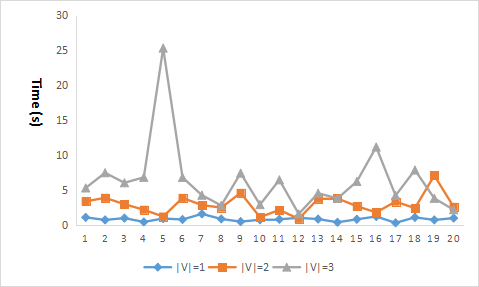
\includegraphics[width=7cm]{chapter04/time_4_12.png}
	}
	\subfigure[$\CTLsnf$子句的个数]{
		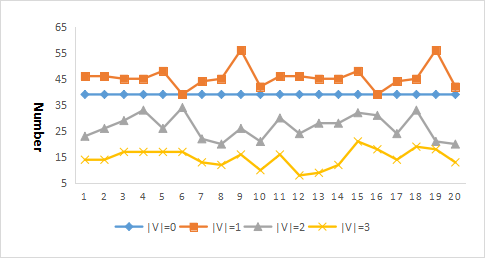
\includegraphics[width=7cm]{chapter04/number-4-12.png}
	}
	\caption{计算{\CTL-forget}$(\varphi, V)$使用的时间和在“移除原子命题”步骤后$\CTLsnf$子句的个数,其中$\varphi_i=12$。}
	\label{chapter04:fig:for12}
\end{figure*}

\begin{figure*}[!htb]
	\centering
	\subfigure[计算遗忘需要的CUP时间]{
		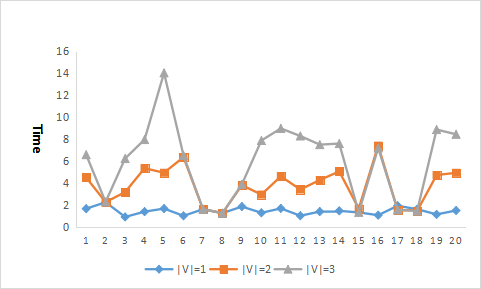
\includegraphics[width=7cm]{chapter04/time_4_16.png}
	}
	\subfigure[$\CTLsnf$子句的个数]{
		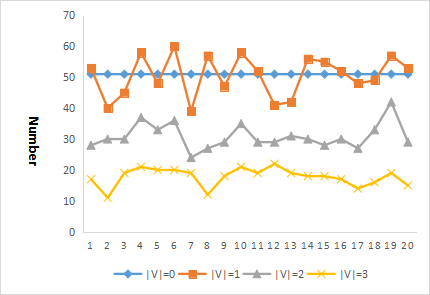
\includegraphics[width=7cm]{chapter04/number-4-16.png}
	}
	\caption{计算{\CTL-forget}$(\varphi, V)$使用的时间和在“移除原子命题”步骤后$\CTLsnf$子句的个数,其中$\varphi_i=16$。}
	\label{chapter04:fig:for16}
\end{figure*}

\subsubsection{SNC计算结果分析}
这部分实验分析使用基于遗忘的方法计算$\CTL$公式的SNC,分为两组实验:计算经典命题公式和$\CTL$公式的SNC,即:计算$q$在$V$和$\varphi \wedge q$上的SNC($\CTLforget(\varphi\wedge q, \Var(\varphi)-V \cup \{q\})$),其中$V\subseteq \Var(\varphi)$、$q\in \Var(\varphi\wedge q)-V$。
这些公式$\varphi$都是随机生成的定义在原子命题集$\Ha$上的公式、$V$是在计算过程中随机生成的、$q\not \in \Var(\varphi)$是一个固定的原子命题且$|\Ha|=50$。

首先测试随机3-CNF命题公式。令$|V|$的取值范围为$\{5,10,\dots, 40,45\}$,3-CNF公式的子句个数$nc$范围为$\{10,15,\dots, 45,50\}$。
在每种情形当中,计算20个随机实例$(\varphi,q,V)$:$\varphi$为$\Ha$上的公式,且$V\subseteq \Var(\varphi)$。
计算SNC的平均CPU时间如图\ref{chapter04:fig:ProTime}所示。

\begin{figure*}[!htb]
	\centering
	\subfigure[平均CPU时间(s)]{
		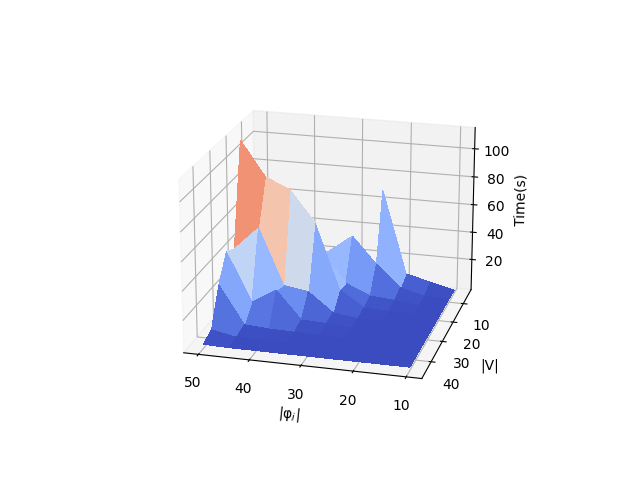
\includegraphics[width=7.5cm]{chapter04/PRototalAveTime.png}
	}
	\subfigure[$|V|=25$时所使用CPU时间箱线图 % and $|\varphi|~\in~ \{10, 15,\dots, 50\}$
	]{
		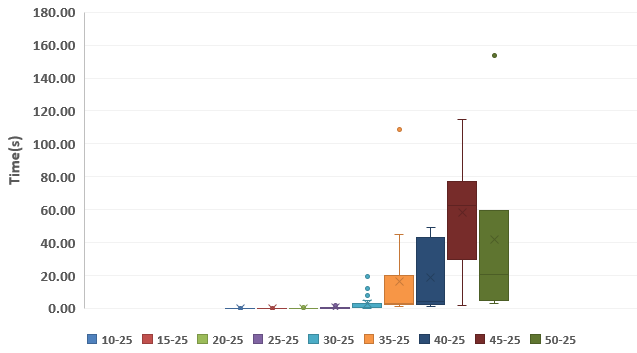
\includegraphics[width=7cm]{chapter04/ProBox(10-50)_25.png}
	}
	\caption{%The performances of computing SNC in PL.
		计算3-CNF公式SNC的CPU时间}
	\label{chapter04:fig:ProTime}
\end{figure*}


从图\ref{chapter04:fig:ProTime}(a)可看出,随着$|\varphi|$增大或$|V|$的减小时间消耗越大。
直观上,若$|\varphi|$越大或者$|V|$越小,则$\CTLforget(\varphi, \overline{V})$越难计算。
这与上一小节中的结论相符合。
图\ref{chapter04:fig:ProTime}(b)展示了当$|V|= 25$、$nc\in \{10,15,\dots, 45, 50\}$时20个随机实例的箱线图。
这同样证明了$nc$越大SNC越难计算。


其次,测试具有如下形式的$\CTL$公式的SNC的计算:
$$\varphi_1 \wedge \ALL \NEXT \varphi_2 \wedge \EXIST\NEXT \varphi_3$$
其中$\varphi_i$($i=1,2,3$)为随机产生的定义在$\Ha$上的3-CNF公式,且满足$|\varphi_1|=|\varphi_2|=|\varphi_3|$。
在这种情形下,每个实例$(\varphi, q, V)$是随机产生的,其中$\varphi=\varphi_1 \wedge \ALL \NEXT \varphi_2 \wedge \EXIST\NEXT \varphi_3$、$V\subseteq \Var(\varphi)$、$|\varphi|\in \{5,6,\dots, 13,14\}$、且$|V|\in \{15,16,\dots, 23,24\}$。
值得注意的是在实例$(\varphi, q, V)$中,$q$可能没有在$V$和$\varphi\wedge q$上的SNC。

图\ref{chapter04:fig:CtlTime}(a)展示了每种情形计算40个实例的SNC的平均CPU时间。与命题公式的情形相似,若$|\varphi|$越大或者$|V|$越小,则$\CTLforget(\varphi, \overline{V})$越难计算。
此外,图\ref{chapter04:fig:CtlTime}(b)展示了每种情形下40个实例中SNC存在的占比,即:$|\varphi|$越小或者$|V|$越小则SNC存在的占比越大。特别地,当$|\varphi_i|=5$且$|V|=16$时,SNC存在的占比为80\%。



\begin{figure*}[!htb]
	\centering
	\subfigure[平均CPU时间(s)]{
		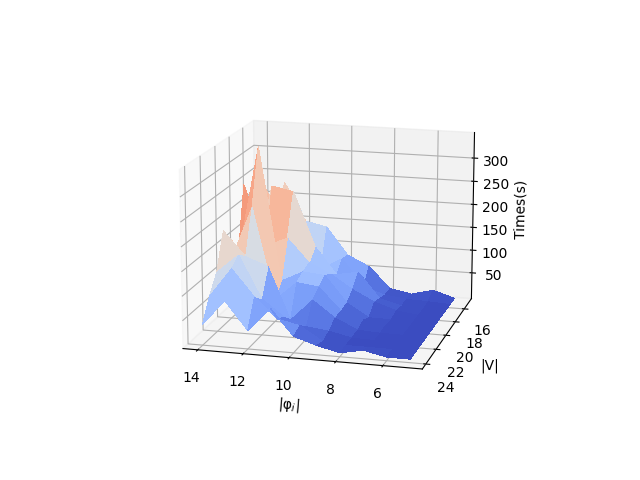
\includegraphics[width=7cm]{chapter04/totalAveTime.png}
	}
	\subfigure[存在SNC的公式占比(\%)]{
		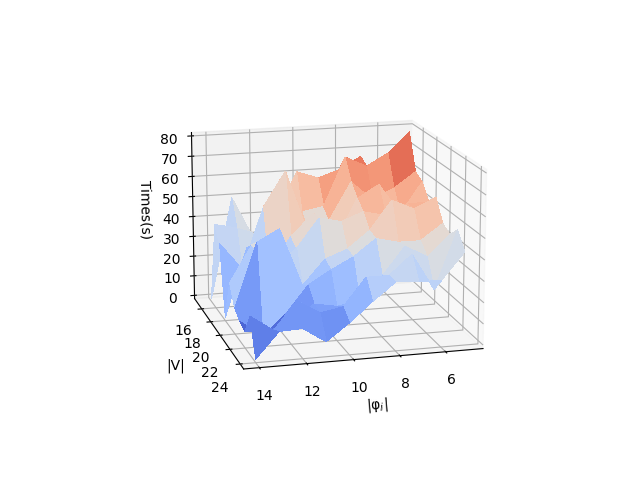
\includegraphics[width=7cm]{chapter04/numPercent.png}
	}
	\caption{计算$\CTL$SNC的平均时间和存在SNC的公式占比.}
	\label{chapter04:fig:CtlTime}
\end{figure*}

综上所述,算法\ref{alg:compute:forgetting:by:Resolution}大多数情况下能计算出SNC(WSC),且当需要遗忘的原子个数很少或公式长度较小时计算效率较高。


\section{本章小结} 
本章第~\ref{chapter05:sec:model}节讨论了一种基于模型的计算约束$\CTL$下遗忘的计算。为此,本章第一节首先提出了一种有界$V$-互模拟概念,并证明了该有界$V$-互模拟与$V$-互模拟在有限结构下是等价的。此外,定义了给定深度的计算树在给定原子命题集上的特征公式,由此定义了有限结构的特征公式。结论表明初始结构能够满足给定的特征公式当且仅当该初始结构与特征公式对应的初始结构在给定原子命题集上互模拟。基于此,得出了任意公式语义等价于其所有模型的特征公式的析取,因而可以计算遗忘的结果。最后,给出了基于模型的计算遗忘算法,并分析该算法关于公式的大小是指数空间的。

本章第~\ref{chapter05:sec:resolution}节探索了如何使用Zhang等人提出的归结系统计算$\CTL$遗忘。为此,首先,使用Zhang提出的转换规则将$\CTL$公式转换成$\CTLsnf$子句集,并使用归结规则在要遗忘的原子命题集上做穷尽的归结;然后,给出几个互模拟等价的等式消除索引,并提出一般化的Ackermann引理用于移除一些新引入的原子命题;最后,给出计算遗忘的算法,并分析该算法的复杂性,分析表明使用该算法计算遗忘的时间和空间复杂性关于公式和要遗忘的原子命题个数是指数时间的。


随后,第~\ref{cha5:subsec:prolog}节给出了基于Proplog的算法$\CTL$-forget实现介绍。第~\ref{cha5:subsec:expriment}节从两个角度来评估算法$\CTL$-forget的系统实现。实验结果表明,从标准数据集中获取的公式和随机产生的公式下,遗忘的计算对需要遗忘的原子命题个数和公式长度都很敏感:要遗忘的原子命题越多或公式越长,计算效率越低。
此外,关于计算SNC的实验表明,算法CTL-forget在用于实验的数据集中,大部分情况是能计算出SNC的。三维图和箱线图都表示计算SNC体现了跟计算遗忘一样的规律,这与SNC是由遗忘来计算是一致的。
 
%
\chapter{CTL下的遗忘理论的定义及其语义属性}\label{chapter03}
{\em 本章首先基于实现差分隐私的随机扰动原理,借鉴Shannon基本通信模型建立差分隐私通信模型。其次,从信息量化的角度,引入信息熵、联合熵、条件熵、互信息及失真函数等量化差分隐私保护前后的隐私信源熵、隐私泄露风险、数据效用。进一步,以此度量模型及方法为基础,针对多维关联属性的隐私量化问题,以关联性分析、关联依赖图模型、马尔可夫模型为理论基础,提出面向关联属性的信息熵度量方法。}

\section{引言}
数据密集型科学研究第四范式\cite{hey2009the},强调数据的重要性。可见,数据已成为支撑决策、人工智能、机器智能、挖掘分析的核心,尤其在普适计算模式下,数据正发挥着重要的价值。然而,随着数据流动,开放共享,用户隐私正在面临严峻的挑战。为解决隐私泄露问题,学术界与产业界开展了一系列积极而有意义的工作。其中,差分隐私(differential privacy,DP)\cite{dwork2006differential,dwork2006calibrating}因具有严格的数学理论支撑,逐步发展成为了隐私保护领域研究的热点。隐私保护的数据发布在差分隐私的诸多应用场景中占据着重要的地位。如在差分隐私的非交互式数据发布中,数据发布者旨在利用差分隐私噪声扰动发布原始数据集的净化版本,将其提供给数据使用者进行分析使用。数据发布势必涉及到隐私泄露与数据效用两方面,因此,对于隐私保护机制的研究,度量(Metrics)是应首要解决的基础性工作。当前,隐私缺乏定量化的定义\cite{Lifenghua16},隐私度量问题,特别是面向多维关联数据情景的隐私度量尚需要进一步研究\cite{ningbowu2019}。%例如,文献\cite{zhu2015correlated}指出由属性关联导致的数据隐私问题。
隐私度量是研究权衡隐私泄露与数据效用\cite{sankar2013utility,kalantari2018robust}解决方案的关键,同时也是隐私泄露风险分析及隐私量化评估的理论基础。 鉴于此,研究隐私度量问题具有重要的理论和实际应用价值。

在隐私度量\cite{alvim2012measuring,wagner2018technical,peng2016,xiongjinbo2018}的研究工作中,基于信息论的量化信息流\cite{smith2009on,boreale2015quantitative,alvim2011on,alvim2010differential}是一种被学者广泛接受的量化方法,受到了研究者的关注。所谓量化信息流就是使用信息熵、条件熵、互信息等概念来度量信息系统中信息流动,它也可以被用于量化一个信息系统中的信息泄露量。标准框架下的量化信息流是基于熵的信息量化,它是熵与信息测量\cite{renyi1961on}的发展。近年来,在解决差分隐私保护模型中隐私泄露与数据效用的权衡问题时,基于信息量化的方法奠定了信息论度量的基础\cite{mir2012information,alvim2011differential,wang2016on}。基于熵的度量是平均意义上的隐私泄露,它属于信息论模型下的差分隐私研究\cite{sarwate2014a}。相比于差分隐私模型\cite{dwork2006differential,dwork2006calibrating},前者的度量对数据分布做出了部分假设 ,而后者没有对数据分布做出任何假设。对数据分布的假设,考虑了数据先验分布的影响,捕捉到了在有些应用中敌手拥有关于数据的先验知识\cite{kalantari2018robust}。 基于上述的原因,从信息熵的角度研究隐私泄露风险与数据效用度量问题,对于隐私泄露风险量化分析和差分隐私最优化机制设计具有重要的理论意义。


目前,信息论方法的隐私度量应用于差分隐私研究,已取得了一定的研究成果。但是,随着系统应用的推进,尚存在一些问题需要进一步研究。当前相关研究工作中对`` 是''和``否''类型的二元对称信道研究较多,逐步发展到类别型数据且多以元组为离散型随机变量构建离散信源模型,较少考虑元组多维属性关联关系且缺少多类型属性组合方面的研究。为此,本文围绕差分隐私的应用,借鉴Shannon基本通信模型\cite{shannon1948a}(参见小节\ref{sec:shannon_comunication_system}介绍)构建差分隐私通信模型。为解决其中的隐私量化问题,本章以通信模型为基本出发点,基于信息熵、失真测度方法提出隐私泄露量化、数据效用量化的方法。然后,在面向多维属性关联的差分隐私数据发布应用中考虑了隐私泄露的信息熵量化方法。通过数据相关度分析,构建关联依赖图模型,进一步,利用图模型中的关键隐私泄露路径,提出面向关联属性的信息熵度量方法。结合数据处理不等式、费诺不等式,给出隐私泄露风险的界。由此,本章所提出的度量方法,奠定信息论方法研究的基础,亦可为隐私泄露风险评估提供基于信息论的理论支撑。

 \section{问题描述}
假设一个数据集$\mathcal{D}$由$n$条数据元组组成($|\mathcal{D}|=n$),其中每个元组包含有$k$个维度的属性,它们是有关特定个体的描述信息。例如,表~\ref{tab:origin} 所示数据集包含Age,Sex,Race等属性信息,医疗数据集包含姓名、血压、体重、疾病等属性。诸如此类的数据集可以表示为$n\times k$的矩阵,其中的行表示元组,列表示属性。本文中,假设离散型随机变量$X_i \in \mathcal{X}_i$表示属性集合$\bm{X}$中的第$i$个属性,$i=1,2,\cdots,k$,由此,$\bm{X}$是一个长度为$k$的随机变量序列,记作$\bm{X}=\{X_1,X_2,\cdots,X_i,\cdots,X_k\}$。进一步,令$|\mathcal{X}_i| = m_i$表示属性$X_i$取值域$\mathcal{X}_i$基数,则有$k$ 属性乘积空间$\mathcal{X}=\prod_{i=1}^{k}\mathcal{X}_i$,基数$m=\prod_{i=1}^{k} m_i$。数据集$\mathcal{D}$是可视为抽样于数据全集$\mathcal{X}^{n}$的多重集,也就是$\bm{X}^{n}$,表示随机变量序列$\bm{X}$的$n$次独立随机抽样。
 基于上述符号的表示,差分隐私非交互式数据发布表示为数据管理者利用发布机制发布原始数据集$\bm{X}^n$的近似副本$\hat{\bm{X}}^n$,以满足隐私保护与数据可用性需求。

目前,针对差分隐私的隐私度量工作中较少考虑多维属性之间存在的关联性依赖。但是,实际的应用场景中,有关个体的多维属性信息之间较少存在相互独立的情况,而且多维属性的相互关联可能会泄露个体的隐私信息。 例如,Age,Occupation与Marital-status的关联,医疗数据集中,血压和体重的相关性增加了疾病敏感信息泄露的风险。基于此,研究面向多维属性关联的隐私度量对于隐私保护机制设计是亟待解决、而又基础和关键的工作。由于数据集中具有多类别属性、相关联的数据结构形式,对其展开隐私度量研究面临的主要问题有:(1) 属性关联识别;(2) 属性相关性表示;(3) 关联属性的隐私度量。围绕这些问题的解决,本章中旨在基于关联分析方法结合信息熵分析属性关联图中隐私泄露关键路径,给出隐私信息熵度量方法。但是,多维混合数据类型给属性相关性分析带来困难,进而,细粒度考虑多属性相关性的隐私度量需要提出新的方法。

\section{差分隐私通信模型}\label{sec:communication_model_of_dp}
差分隐私的标准定义形式\ref{def:dp},约束随机化函数$Q$在输出空间$S$上满足概率性输出的$\epsilon$-不可区分性。本质上,实现差分隐私的随机化函数$Q$ 与\ref{sec:shannon_comunication_system}小节Shannon信息论噪声信道数学模型$\left \{X~Q(\hat{X}|X)~\hat{X}\right \}$的转移条件概率矩阵$q(\hat{x}|x)$ 表示具有相似之处。以此为基础,差分隐私接受输入原始数据$X^n$,噪声扰动输出净化合成数据集$\hat{X}^n$,从信息论的角度借鉴通信系统模型\ref{sec:shannon_comunication_system}建立差分隐私的基本通信模型。其中,原始数据假设为隐私信源$\bm{X}$、 输出数据为信宿$\hat{\bm{X}}$,差分隐私随机化机制抽象为噪声信道$Q$,如图\ref{fig:chapter04-communication_of_dp}描绘了差分隐私随机化映射$Q$的通信模型。

 \begin{figure}[htbp]
 	\centering
 	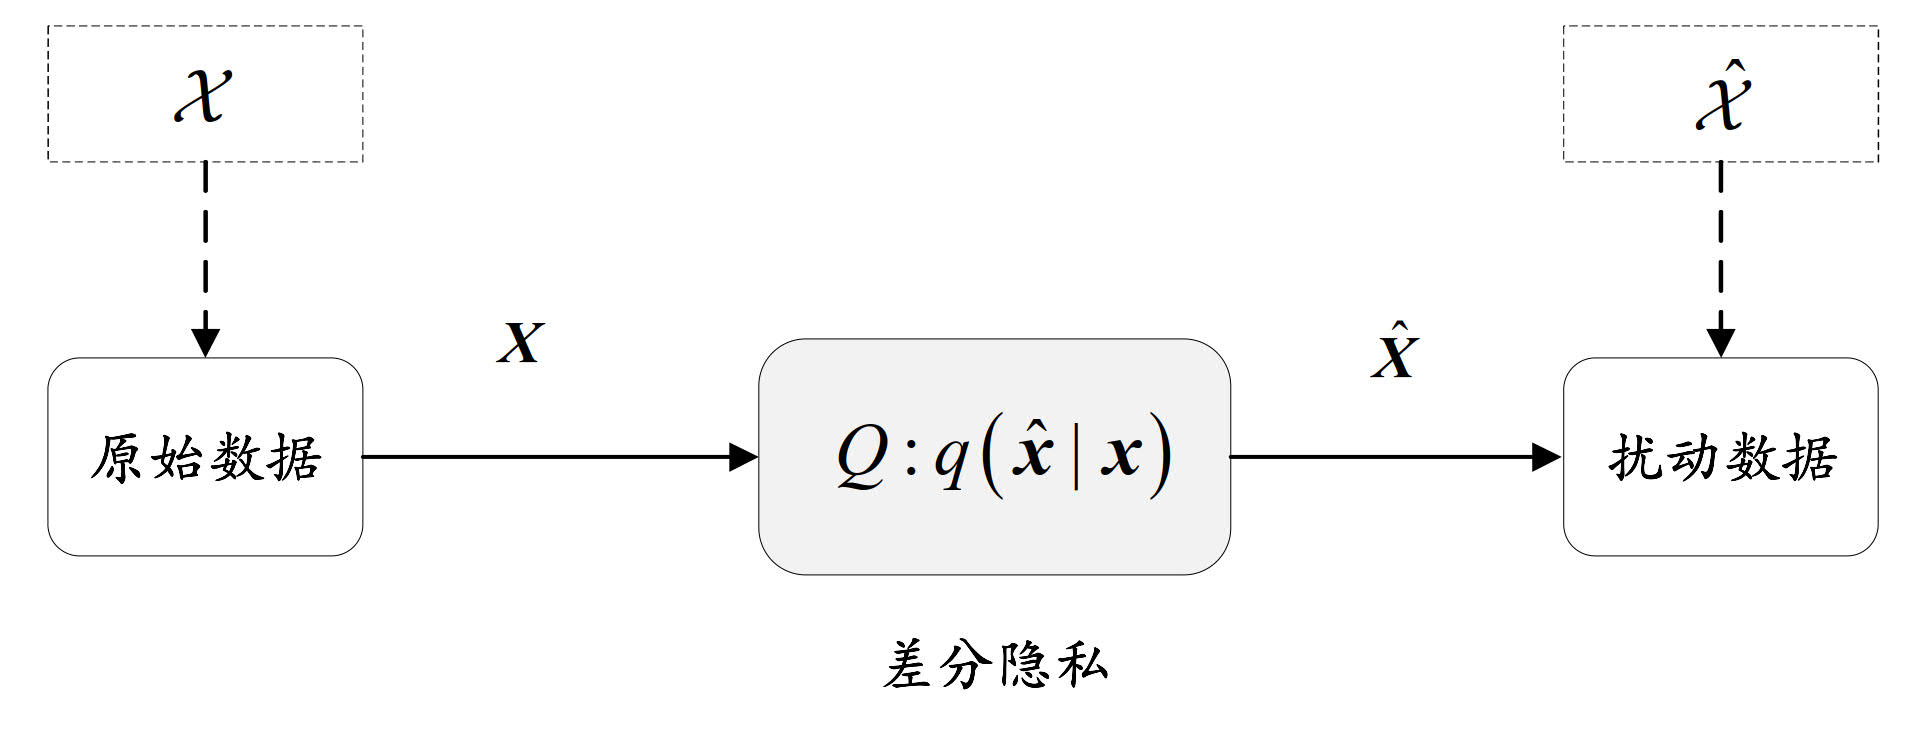
\includegraphics[width = 0.65\linewidth]{./figures/chapter04_1.jpg}
 	\caption{差分隐私的基本通信模型}
 	\label{fig:chapter04-communication_of_dp}
 \end{figure}


  以上述信道模型$\left \{\bm{X}~Q(\hat{\bm{X}}|\bm{X})~\hat{\bm{X}}\right \}$为基础,本章给出差分隐私的一个等价定义。不失一般性,假设输入数据$\bm{x}$取值于离散型字母表$\bm{x}\in \mathcal{X}$,输出数据$\hat{\bm{x}}$来源于字母表$\hat{\bm{x}} \in \hat{\mathcal{X}}$,如此,差分隐私形成一个噪声信道$Q$,随机概率性映射$Q:\mathcal{X}\rightarrow \hat{\mathcal{X}}$。基于这样的信道模型假设,差分隐私可以被正式的定义为如下的表述形式\cite{alvim2011differential}。

 \begin{definition}\label{def:dp_channel}假设$\mathcal{X}$和$\hat{\mathcal{X}}$为离散有限集合,分别表示原始数据输入和扰动数据输出字母表。如果一个随机化概率性映射$Q:\mathcal{X}\rightarrow \hat{\mathcal{X}}$满足$\epsilon$-差分隐私,当且仅当条件概率$q(\cdot|\cdot)$满足
 	\begin{equation}
 		q(\hat{\bm{x}}|\bm{x})\leq \exp(\epsilon) \cdot q(\hat{\bm{x}}|\bm{x}') \quad  \forall \hat{\bm{x}} \in \hat{\mathcal{X}}, \bm{x},\bm{x}' \in \mathcal{X}, \bm{x}\sim \bm{x}'
 	\end{equation}
 其中,隐私参数$\epsilon^* = \min\left\{\epsilon:q(\hat{\bm{x}}|\bm{x})\leq \exp(\epsilon) \cdot q(\hat{\bm{x}}|\bm{x}')\right\}$。
 \end{definition}

基于上述定义\ref{def:dp_channel},差分隐私直接表述为噪声信道条件概率矩阵的特性,采用$\log \frac{q(\hat{\bm{x}}|\bm{x})}{q(\hat{\bm{x}}|\bm{x}')}$量化差分隐私保护强度。对此定义,给出以下两点解释说明。首先,上述差分隐私定义提供了数据分布独立的隐私保障,$\epsilon$-隐私度量仅依赖于信道条件概率$q(\hat{\bm{x}}|\bm{x})$。其次,对于有限的$\epsilon > 0$,概率矩阵中相同输出元素$\hat{\bm{x}}$的条件概率不可能同时存在零和非零的概率。除此之外,$\bm{X}$与$\hat{\bm{X}}$之间的相关度测量给定$\hat{\bm{X}}$时有关$\bm{X}$的隐私泄露信息量,$\bm{X}$与$\hat{\bm{X}}$ 之间的失真程度$d(\bm{X},\hat{\bm{X}})$测量数据质量损失。以此为基础,本章中\ref{sec:information_theoretic_metrics}节给出差分隐私机制的信息熵度量模型及方法。



\section{隐私与效用度量}\label{sec:information_theoretic_metrics}
基于上述\ref{sec:communication_model_of_dp}节介绍的差分隐私通信模型,接下来,从量化信息流的角度,本章利用信息熵、互信息、失真函数等概念分别给出隐私信源、隐私泄露风险、数据效用的度量方法,为后续研究奠定度量基础。

\subsection{隐私信源熵}
信息熵的定义\ref{def:entropy}描述了隐私信源的不确定程度,它刻画了消除隐私信源不确定度平均需要的信息量,由此,信息熵也可表达隐私信源的平均隐私信息量。针对单属性情景,将其视为离散随机变量$X_i$,具有$m_i$个不同的元素$\alpha_u,u=1,2,\cdots,m_i$。由此,隐私信源数学模型定义为
\begin{equation}
\begin{pmatrix}
X_i\\
P(X_i)
\end{pmatrix}=\begin{Bmatrix}
\alpha_{1}, & \alpha_{2}, & \cdots, & \alpha_{u}, & \cdots,  & \alpha_{m_i}\\
p(\alpha_{1}),& p(\alpha_{2}), & \cdots, & p(\alpha_{u}), & \cdots, & p(\alpha_{m_i})
\end{Bmatrix}
\end{equation}
$0 \leq p(\alpha_u) \leq 1$,$\sum_{u=1}^{m_i}p(\alpha_u)=1$,则隐私信源熵$H(X_i)=-\sum_{u=1}^{m_i}p(\alpha_u) \log p(\alpha_u)$。
进一步,推广应用到~$k$~维属性情景时,概率空间为数据集域值空间的$m$种所有可能组合。信源$\bm{X}$的概率模型表示为~$k$~维属性联合概率分布
\begin{equation}
	\begin{pmatrix}
		\bm{X}\\
		P(\bm{X})
	\end{pmatrix}=\begin{Bmatrix}
		\beta_{1}, & \beta_{2}, & \cdots,  & \beta_{v}, & \cdots,  & \beta_{m}\\
		p(\beta_{1}),& p(\beta_{2}), & \cdots, & p(\beta_{v}), & \cdots, & p(\beta_{m})
	\end{Bmatrix}
\end{equation}
$0 \leq p(\beta_v) \leq 1$,$\sum_{v=1}^{m}p(\beta_v)=1 (v=1,2,\cdots,m)$。$\beta_v \in \{\alpha_{u_1},\alpha_{u_2},\cdots,\alpha_{u_i}\},1\leq i \leq k, 1\leq u_i \leq m_i$是一个$k$元组,其中元组的第$i$个分量是随机变量$X_i$的某个具体取值$\alpha_u$。基于此,$k$维属性的联合信源熵表示为随机变量序列的联合熵,记作$H(\bm{X}) = H(X_1,X_2,\cdots,X_k)$。依据熵的链式法则(定理\ref{theorm:multi_joint_entropy_}中公式\ref{eq:joint_entropy}),则有多属性联合信源熵
\begin{alignat}{2}
	H(\bm{X}) & = H(X_1,X_2,\cdots,X_k) \\
	& = -\sum_{x_1,x_2,\cdots, x_k} p(x_1,x_2,\cdots, x_k)\log p(x_1,x_2,\cdots, x_k)\\
	& = -\sum_{x_1,x_2,\cdots, x_k} p(x_1,x_2,\cdots, x_k)\log \prod_{i=1}^{k}p(x_i|x_{i-1},\cdots,x_1)\\
	& = \sum_{i=1}^{k}H(X_i|X_{i-1},\cdots,X_1)\label{eq:chapter03-7}
\end{alignat}



事实上,多维属性之间相互独立是属性关联的一种特例情况,属性独立时的联合概率$P(\bm{X}=\bm{x})=\prod_{i=1}^{k} P(X_i=x_i)$,条件概率$p(x_i|x_{i-1},\cdots,x_1)=p(x_i)$成立。由公式~\ref{eq:chapter03-7}易知,元组属性相互独立时,$k$维属性联合$\bm{X}=\{X_1,X_2,\cdots,X_i,\cdots,X_k\}$的信源熵$H(\bm{X})$满足可加性,表示为
\begin{equation}
	H(\bm{X})=\sum_{i=1}^{k}H(X_i)
\end{equation}
多维属性联合信源熵$H(\bm{X})$量化了个体隐私信息的不确定度,从元组整体上对隐私属性信息进行度量。如果数据集元组独立同分布的抽样于数据取值字母表集合,则可以使用
离散平稳无记忆信源的$n$次扩展信源模型表达扩展后的隐私信源模型,记作$\bm{X}^{n}$表示信源$\bm{X}$的$n$次扩展。信源$\bm{X}^{n}$数学模型表示为

\begin{equation}
	\begin{pmatrix}
		\bm{X}^n\\
		P(\bm{X}^n)
	\end{pmatrix}=\begin{Bmatrix}
		\vec{x}_{1}, & \vec{x}_{2}, & \cdots,  & \vec{x}_{i}, & \cdots , & \vec{x}_{m^n}\\
		p(\vec{x}_{1}),& p(\vec{x}_{2}), & \cdots,& p(\vec{x}_{i}), & \cdots, & p(\vec{x}_{m^n})
	\end{Bmatrix}
\end{equation}
其中的$p(\vec{x}_{i})=\prod_{j=1}^{n}p(x_{i_j})$表示$n$个符号消息序列的联合概率。由此,根据熵的定义\ref{def:entropy},离散无记忆信源$X$的$n$次扩展信源熵$H(X^n)$可表示为
\begin{alignat}{2}
	H(\bm{X}^{n})  &=  -\sum_{X^n}p(\vec{x}) \log p(\vec{x}) \\
	& =  -\sum_{X^n}\left(\prod_{j=1}^{n}p(x_{i_j})\log \prod_{j=1}^{n}p(x_{i_j})\right)\\
	& = -n\sum_{i=1}^{m}\sum_{j=1}^{n}p(x_{i_j}) \log p(x_{i_j}) \\
	& = nH(X_1,X_2,\cdots,X_k)\\
	& =n\sum_{i=1}^{k}H(X_i|X_{i-1},\cdots,X_1)
\end{alignat}

%通常非独立的情景下,联合熵的计算依据熵的链式法则(定理\ref{theorm:multi_joint_entropy_}中公式\ref{eq:joint_entropy}),在此不再过多的赘述。
隐私信源熵度量了原始隐私信息的平均不确定量,表达了信源消除不确定度平均所需要的比特数,刻画了隐私信源特征。
\subsection{隐私泄露风险}
本章中考虑隐私攻击者或敌手可以观察到信道输出结果,在这样的敌手模型下,隐私攻击者观察噪声信道输出$\hat{\bm{X}}^n$后对信源消息$\bm{X}^n$仍具有的不确定度可以使用条件熵$H(\bm{X}^n|\hat{\bm{X}}^n)$度量。首先,$n$次扩展信源$\bm{X}^n$经差分隐私构成离散无记忆信道$\{\bm{X}~Q(\hat{\bm{X}}|\bm{X})~\hat{\bm{X}}\}$的$n$次扩展信道模型,条件概率满足$q(\bm{X}^{n}|\hat{\bm{X}}^n)=\prod_{i=1}^{n}q(\bm{X}^i|\hat{\bm{X}}^i)$。由此采用条件熵定义的平均隐私熵$E$满足
\begin{equation}
	E=\frac{1}{n}H(\bm{X}^{n}|\hat{\bm{X}}^n) = -\frac{1}{n}\mathbb{E} \log q(\bm{X}^{n}|\hat{\bm{X}}^n)= -\frac{1}{n}\mathbb{E} \log \prod_{i=1}^{n}q(\bm{X}^i|\hat{\bm{X}}^i)
\end{equation}
故有,
\begin{equation}
	E= -\frac{1}{n}\sum_{i=1}^{n}\mathbb{E} \log q(\bm{X}^i|\hat{\bm{X}}^i) = \frac{1}{n}\sum_{i=1}^{n}H(\bm{X}^i|\hat{\bm{X}}^i)
\end{equation}
鉴于此,得到平均隐私熵
\begin{equation}
	E=  -\frac{1}{n}\sum_{i=1}^{n}\left(\sum_{\bm{x} \in \mathcal{X}}\sum_{\hat{\bm{x}} \in \hat{\mathcal{X}}}p(\bm{x},\hat{\bm{x}})\log q(\bm{x}|\hat{\bm{x}})\right)
\end{equation}

依据熵与互信息的关系(参见\ref{sec:entropty_mutual_information}小节),互信息量可用于度量$\hat{\bm{X}}^{n}$含有信源$\bm{X}^n$的信息量。本质上,条件熵与互信息的度量可以平等对待,本章中利用互信息$I(\bm{X}^{n};\hat{\bm{X}}^{n})$的含义定义隐私泄露风险函数$L(\bm{X}^{n},\hat{\bm{X}}^{n})$量化平均意义上的隐私泄露量
\begin{alignat}{2}
	L(\bm{X}^{n},\hat{\bm{X}}^{n}) & = \frac{1}{n}I\left(\bm{X}^{n};\hat{\bm{X}}^{n}\right)\\
	& = \frac{1}{n}\left(H(\bm{X}^{n})-H(\bm{X}^{n}|\hat{\bm{X}}^{n})\right)\label{eq:privacy_leakage_risk}\\
	&=\frac{1}{n}\left (nH(\bm{X})-\sum_{\bm{X},\hat{\bm{X}}}H(\bm{X}|\hat{\bm{X}})\right )\\
	& \leq H(\bm{X})-\frac{1}{n}\sum_{\bm{X},\hat{\bm{X}}}H(\bm{X}|\hat{\bm{X}})
\end{alignat}
借鉴离散无记忆信道$n$次扩展信道的重要结论,信道输出变量仅依赖于输入变量与其它变量条件独立,则有$	L(\bm{X}^{n},\hat{\bm{X}}^{n})=\frac{1}{n}\sum_{\bm{X},\hat{\bm{X}}}I(\bm{X};\hat{\bm{X}})=I(\bm{X};\hat{\bm{X}})$。互信息隐私泄露风险是平均意义上的隐私泄露度量,它可以被解释成为一个敌手在平均意义上需要的比特数,用于完全的识别出特定的个体数据\cite{oya2017back}。由上述公式\ref{eq:privacy_leakage_risk} 可知,固定信源分布,$L(\bm{X}^{n},\hat{\bm{X}}^{n})$与$H(\bm{X}^{n}|\hat{\bm{X}}^{n})$负相关。由于互信息是信源分布和条件概率分布的函数,该测量在信息论的差分隐私模型中得到了广泛的应用。

\subsection{数据效用量化}

为解决损失压缩问题,Shannon信息论引入了失真测量函数,量化随机变量和它的表示之间的失真程度\cite{cover2006elements}。受此启发,本章中数据效用度量差分隐私噪声信道输出合成数据集副本与原始数据集的失真距离,也就是数据质量。采用非负的失真函数$d(\bm{X}^{n},\hat{\bm{X}}^{n})\rightarrow \mathbb{R}^{n}$量化原始输入与扰动输出的失真程度,测量发布数据的可用性,定义期望失真
\begin{equation}\label{eq:chapter03-ED}
\mathbb{E}\left[d(\bm{X},\hat{\bm{X}})\right]=\sum_{\bm{x},\hat{\bm{x}}}p(\bm{x})q(\hat{\bm{x}}|\bm{x})d(\bm{x},\hat{\bm{x}})
\end{equation}
量化平均意义上的失真程度。失真测量中的汉明失真($d(\bm{x},\hat{\bm{x}})=1,\bm{x} \neq \hat{\bm{x}}; d(\bm{x},\hat{\bm{x}})=0, \bm{x}=\hat{\bm{x}}$)是一种严格的失真测量,称为示性函数,具有灵敏度高的特点,对于具有明确含义的类别型数据特别有意义。由汉明失真可以得到一个误差概率失真\cite{cover2006elements}
\begin{equation}\label{eq:expected_hamming_distortion}
	\mathbb{E}\left[d(\bm{X},\hat{\bm{X}})\right]={\rm Pr}\left\{\bm{X} \neq \hat{\bm{X}}\right\}
\end{equation}
%度量合成数据集与原始输入数据集序列的失真程度,衡量集的整体可用性。由于数据集混合数值型与类别型属性,通常总是假设$\mathcal{X}=\mathcal{\hat{X}}$。


%度量输入与输出序列对应位置不同符号数目, 其优势在于无论差分隐私机制输入与输出符号改变多小,基于汉明失真的效用度量能够维持较高的灵敏度,尤其对于类别型数据很有意义。此外,平均意义的汉明失真度量发布合成数据集与原始数据集的平均失真程度,定义发布合成数据集的期望汉明失真函数


其中${\rm Pr}\left\{\bm{X} \neq \hat{\bm{X}}\right\}$表示$\bm{X}$与$\hat{\bm{X}}$之间的误差概率。因失真的度量方法比较直观、且具有降低计算复杂性的优势\cite{oya2017back},它已经被应用在差分隐私的相关研究工作中量化数据效用(如文献\mycite{andres2013geo,kalantari2018robust,sarwate2014a,wang2016on})。文中基于期望汉明失真,从隐私信源分布、噪声信道条件概率、扰动输出数据的方面量化差分隐私保护系统平均情况下的数据失真程度,实现发布合成数据与原始数据之间的效用度量。
\section{关联属性隐私度量模型及方法}
上述\ref{sec:information_theoretic_metrics}小节,讨论了信息论方法量化隐私与效用的一般性理论。接下来,将上述结论推广到多维属性关联的差分隐私应用场景,以下从关联属性相关度量化、关联依赖图模型表达、数据关联的隐私度量方面展开叙述。
\subsection{关联属性相关度}\label{sec:correlation_inditifity}
数据集$\mathcal{D}$中元组有$k$个属性,由随机变量序列$\bm{X}=\{X_1,X_2,\cdots,X_i,\cdots,X_k\}(1 \leq i \leq k)$表示个体数据信息。通常情况下,$k$ 个属性并不相互独立,而是存在数据的关联。如果存在$l(1 <k)$ 个属性与$X_i$属性关联,则称它们是一个关联属性组,记作$\bm{R}_i=\{X_i,X_j \in \bm{X}\mid$ 属性集合中与属性$X_i$具有关联关系的属性$X_j\}$。

为了表达多维属性的关联,首先给出属性关联的相关度分析方法。利用相关性分析方法对属性集合$\bm{X}$中属性依次分析属性对$(X_i;X_j)$,$X_i \neq X_j$ 之间的相关度。假设$m_i$,$m_j$分别表示属性$X_i$,$X_j$的基数,$z_{ij}$表示属性$X_i$与$X_j$ 的二维联合频率矩阵中第$i$个元素和第$j$个元素的频率统计值。则基于上述符号表示,可以得到一个具有$m_i \times m_j$个元素的二维属性联合频率表,如下表\ref{tab:table_frquence_4.1}所示。

\begin{table*}[htb]
\small
\centering
\caption{二维属性联合频率表}
\label{tab:table_frquence_4.1}
\begin{tabular}{p{2cm}p{2cm}p{2cm}p{2cm}p{2cm}}
\hline\noalign{\smallskip}
&$X_j(1)$  &$X_j(2)$ &$\cdots$ & $X_j(m_j)$\\
\noalign{\smallskip}\hline\noalign{\smallskip}
$X_i(1)$ & $z_{11}$ & $z_{12}$ & $\cdots$ & $z_{1m_j}$\\
$X_i(2)$ & $z_{21}$ & $z_{22}$ & $\cdots$ & $z_{2m_j}$\\
$\vdots$ & $\vdots$ & $\vdots$ & $\vdots$ & $\vdots$\\
$X_i(m_i)$ & $z_{m_i1}$ & $z_{m_i2}$ & $\cdots$ & $z_{m_im_j}$\\
\noalign{\smallskip}\hline
\end{tabular}
\end{table*}

基于上述表\ref{tab:table_frquence_4.1},属性联合概率分布$P_{ij}=P(X_i=i,X_j=j)$,表示$X_i$属性域中第$i$个值和属性$X_j$ 属性域中第$j$个值同时发生的事件频率。进一步,$P_{i\cdot}$和$P_{\cdot j}$分别表示$X_i$和$X_j$的边缘概率分布,则有,$P_{i\cdot}=\sum_{j}P_{ij}$和$P_{\cdot j}=\sum_{i}P_{ij}$。此外,在相关性分析方法上,Shanon互信息量化了两个随机变量之间的信息相关性,是一种相关性分析方法。对比与其它统计学上的相关性分析方法,互信息可以克服线性和非线性关系的局限性\cite{liangjy2016,reshef2011detecting},在敏感度方面具有较好的优势。基于此,本章中利用互信息方法测量属性集合中任意两者之间的相关性。正式的,定义属性$X_i$,$X_j$之间的相关度为互信息量,根据互信息量的计算公式
\begin{equation}\label{eq:mi_correlation}
	I(X_i;X_j)=\sum_{i=1}^{m_i}\sum_{j=1}^{m_j}P_{ij}\log \frac{P_{ij}}{P_{i \cdot}\cdot P_{\cdot j}}
\end{equation}
进行属性对的相关度分析,为后续多属性关联的属性依赖图表达奠定基础。接下来,给出具体的依赖图构建细节描述。
\subsection{关联属性图模型}
数据集$\mathcal{D}$中属性对$(X_i,X_j),1\leq i,j \leq k$的相关度表达出了元组属性的近似关联依赖强度,依据公式\ref{eq:mi_correlation}计算属性间的互信息量可以得到任意两属性的相关度。结合互信息性质,首先给出以下定理,为下文依赖图处理奠定基础。


\begin{theorem}\label{theorem:chapter04_2.1}
	对于相互关联的属性对$(X_i,X_j)$,互信息量$I(X_i;X_j)$表达为相关度$\theta_{ij}$,$I(X_j;X_i)$表达为相关度$\theta_{ji}$,则有$\theta_{ij}$,$\theta_{ji} \geq 0$ 和 $\theta_{ij}=\theta_{ji}$。
\end{theorem}

上述定理\ref{theorem:chapter04_2.1}的证明利用互信息的对称性、非负性质,本文中不再过多赘述其证明过程。

\begin{corollary}\label{cor:chapter04_2.2}如果属性$X_i$,$X_j$之间的相关度$\theta_{ij}=\theta_{ji}=0$,则属性对$(X_i,X_j)$相互独立,即是$X_i$,$X_j$之间满足$P(X_i,X_j)=P(X_i)P(X_j)$。
\end{corollary}

针对元组属性集合$\bm{X}=\{X_1,X_2,\cdots,X_k\}$,利用互信息的相关性分析方法,得到$(X_i,X_j),1\leq i,j \leq k$之间的相关度。首先,定义关联依赖图$G(V,E)$表达属性关联依赖,其中,$V$表示图中的顶点集合,$E$表示属性之间关联依赖构成的边集合。由于互信息的对称性,$X_i$与$X_j$之间的边$X_i-X_j$是无向边,则图$G(V,E)$是无向图。为表达属性对$(X_i,X_j)$之间的关联依赖强度$\theta_{ij}$,定义顶点$X_i$到$X_j$的边$X_i-X_j$的权值构成带权无向图$G$。其次,利用图的标准表示方法,对数据集属性关联依赖图$G(V,E)$采用邻接矩阵的形式表示,以下给出带权无向图$G$的邻接矩阵$\Theta$定义。


\begin{definition}带权无向图$G$中的顶点序列化$1,2,\cdots,k$,图$G$的邻接矩阵表示为$k$阶矩阵$\Theta$,矩阵元素$\Theta[i][j]$满足
	
	\begin{equation}
		\Theta[i][j]=
		\begin{cases}
			0 & \text{$\theta_{ij} < \omega $}\\ % 需要强制换行
			\theta_{ij} & \text{$\theta_{ij} \geq \omega $}
		\end{cases}
		\text{$1 \leq i,j \leq k$}
	\end{equation}
其中,$\theta_{ij}$为$X_i$与$X_j$的相关度$I(X_i;X_j)$,$\omega$为设置伪相关的阈值门限参数。
\end{definition}

依据推论\ref{cor:chapter04_2.2},邻接矩阵$\Theta$中元素$\Theta[i][j]=0$表示无相关的独立属性$X_i$和$X_j$。基于上述\ref{sec:correlation_inditifity}节中的数据集相关属性分析方法,可以用上述相关度邻接矩阵$\Theta$表达出属性集合中的相关属性关联程度。结合互信息量的对称性、非负性特点\cite{shannon1948a},易知邻接矩阵$\Theta$是对角线元素为$0$的对称矩阵。


\begin{algorithm}[htb]
 \small
 \setstretch{1.2}
\caption{ 图$G$的邻接矩阵$\Theta$生成算法}
\label{alg:gen_Theta}
\begin{algorithmic}[1]
\REQUIRE ~~\\
	\begin{tabular}[t]{p{1mm}l}
	 $\mathcal{D}$&:数据集\\
	 $\bm{X}$&:属性$\{X_1,X_2,\cdots,X_i,\cdots,X_k\}$\\
	 $k$&:属性维度\\
	 $\omega$&:阈值参数
	\end{tabular}
	\ENSURE ~~\\
	\begin{tabular}[t]{p{1mm}l}
	$\Theta$&: 图$G$邻接矩阵
	\end{tabular}
\STATE 初始化图$G$邻接矩阵$\Theta$元素
\FOR{$i=1,\cdots,k$}
\FOR{$j=1,\cdots,i$}
\STATE 设置矩阵元素$\Theta_{ij}=\Theta_{ji}=0$~/*初始属性独立*/
\ENDFOR
\ENDFOR
\FOR{$i=1,\cdots,k$}
\STATE 设置$V=\bm{X}\setminus\{X_i\}$实现属性的依次分析
\FOR{对于$V$中的每一个属性$X_j$}
\STATE 利用数据集$\mathcal{D}$,依据互信息量公式\ref{eq:mi_correlation}计算$\theta_{ij}=I(X_i;X_j)$
\STATE /*过滤伪相关或弱相关的属性关系*/
\IF{$\theta_{ij} \geq \omega$}
\STATE 赋值邻接矩阵元素$\Theta_{ij}=\Theta_{ji}=0$
\ENDIF
\ENDFOR
\ENDFOR
\RETURN 图$G$的邻接矩阵$\Theta$
\end{algorithmic}
\end{algorithm}


算法\ref{alg:gen_Theta}中的伪代码描述了通过数据集关联属性相关度分析,生成带权无向图$G$邻接矩阵$\Theta$的过程。以下给出算法计算过程分析,首先,算法初始化邻接矩阵$\Theta$中元素$\Theta_{ij}=0$对所有的$ 1\leq i,j \leq k$,矩阵初始化状态表示数据集中属性之间相互独立(算法\ref{alg:gen_Theta}中$1 \sim 6$行)。其次,算法依次计算属性对$(X_i,X_j)$之间的互信息量$I(X_i;X_j)$,并根据阈值$\omega$过滤属性边$X_i-X_j$集合,设置图$G$中无向边的权值$\theta_{ij}$(算法\ref{alg:gen_Theta}中的$7 \sim 16$行)。 最后,算法输出属性关联带权无向图$G$的邻接矩阵$\Theta$。

\begin{remark}
{\em 上述算法\textup{\ref{alg:gen_Theta}}的计算开销主要是计算互信息的关联属性相关度,算法的复杂度是数据集属性维度规模$k$的函数,计算输出属性关联带权无向图$G$邻接矩阵$\Theta$的计算时间复杂度为$O(k^2)$,是一个多项式时间算法。此外,在空间复杂度方面,图$G$的邻接矩阵$\Theta$是满足主对角线元素$\Theta_{ij}=0$的$k$阶对称矩阵,采用矩阵的压缩存储可将$\Theta$存储到$\frac{k(k-1)}{2}$个单位存储空间。}
\end{remark}
\subsection{关联属性隐私度量}
基于以上分析,本小节中阐述利用关联依赖图模型度量关联属性隐私的方法。首先,在属性依赖图$G(V,E)$中考虑和敏感属性$X_h$,取值域基数$|\mathcal{X}_h|=m_h$,具有直接相连边的属性组$\bm{R}_{h}$。 假设关联属性组$\bm{R}_{h}$是数据发布者和其它用户已知的非敏感数据知识,隐私获取者可通过其它途径获取的辅助知识。针对此,考虑敏感属性$X_h$通过差分隐私信道编码随机输出$\hat{X}_h$的情况,则有$X_h$与$\hat{X}_h$之间构成的信道特性,表示为条件概率依赖关系$Q:\mathcal{X}_h\rightarrow\hat{\mathcal{X}}_h$。基于上文\ref{sec:communication_model_of_dp}小节中的差分隐私通信模型的信道数学模型,扰动输出的数据边缘分布仅依赖于条件概率分布和敏感属性$X_h$的分布,条件独立于关联属性组$\bm{R}_{h}$,则有
\begin{theorem} \label{theorem:chapter04_markov_graph}
	无向图$G=(V,E)$中,敏感属性顶点$X_h \in V$及其关联属性组$\bm{R}_h\subset V$,与差分隐私信道$X_h \xrightarrow{Q} \hat{X}_{h}$输出$\hat{X}_{h}$之间的概率性依赖构成马尔可夫隐私链$\bm{R}_{h}\rightarrow X_{h}\rightarrow\hat{X}_{h}$的关系。
\end{theorem}

上述定理\ref{theorem:chapter04_markov_graph}结合差分隐私数据处理阐述了图$G$中由关联而存在的马尔可夫隐私链关系。其中,关联属性组$\bm{R}_{h}$的联合概率是初始的概率分布,条件概率$P(X_{h}|\bm{R}_{h})$表达了关联属性组对敏感属性$X_h$的影响,刻画了$X_h$与$\bm{R}_h$之间的条件性依赖。基于此,考虑差分隐私机制$Q$具有条件转移概率$Q(\hat{X}_h|X_h)$的形式,从信息论的角度使用条件概率$q(\hat{x}_{h}^{j}|x_{h}^{i})$表示隐私敏感属性$X_h$取值域$\mathcal{X}_h$ 中第~$i$~个原子符号转移输出域$\mathcal{\hat{X}}_h$中第~$j$~个原子符号的概率。由此,根据定义\ref{def:dp_channel},差分隐私机制$Q$满足概率不可区分条件的最小预算参数$\epsilon^*$,
则有
\begin{equation}\label{eq:epsilon_2.10}
	\epsilon^{*}=\min_{q(\hat{x}_h|x_h)}\log \left(\frac {q(\hat{x}_{h}^{j}|x_{h}^{i})}{q(\hat{x}_{h}^{j}|x_{h}^{t})}\right) \qquad \forall x_h^i \neq x_h^t, x_h^i , x_h^t\in \mathcal{X}_h
\end{equation}

基于上述表达,给出信息熵的度量与分析。首先,隐私泄露风险计算公式\ref{eq:privacy_leakage_risk}是隐私攻击者观察扰动输出$\hat{X}_h$后获得有关敏感信息$X_h$的互信息量$I(\hat{X}_h;X_h)$。结合数据关联的隐私链关系,依据数据处理不等式定义\ref{def:dataprocessinginequality},则有关联属性组$\bm{R}_h$ 与敏感属性$X_h$之间的互信息量$I(\bm{R}_h;X_h)$满足$I(\bm{R}_h;\hat{X}_h) \leq I(\bm{R}_h;X_h)$,即是隐私关联属性组$R_h$和$\hat{X}_h$的隐私信息上界。当$X_h$和$\hat{X}_h$之间相互独立时,类似于通信系统中断,$I(\bm{R}_h;\hat{X}_h)$信息量达到最小值$0$。其次,对于满足期望失真度$D={\rm Pr}\{X_h \neq \hat{X}_h\}$的差分隐私试验信道,互信息隐私泄露量$I(X_h;\hat{X}_h)$满足
\begin{alignat}{2}
	I(X_h;\hat{X}_h) & =H(X_h)-H(X_h|\hat{X}_h) \label{eq:entropty_2.10}\\
	 & = H(X_h)-H(D)-D\log(m_h-1) \label{eq:2.11}
\end{alignat}

对于属性域$\mathcal{X}_h = \hat{\mathcal{X}}_h$时,依据费诺不等式的推论\ref{cor:chapter02-1}易证公式\ref{eq:2.11}。基于互信息的隐私泄露度量依赖于差分隐私噪声信道转移概率$Q(\hat{X}_h|X_h)$和数据先验概率分布。此外,基于失真的数据效用度量公式\ref{eq:expected_hamming_distortion}演变为信道的误差概率,则有
$D={\rm Pr}\{X_h\neq \hat{X}_h\}$。误差概率量化了差分隐私噪声信道输入原始数据$X_h$与扰动输出数据$\hat{X}_h$之间的期望汉明失真度。由此可见,数据效用度量表达了差分隐私概率信道的统计特性。
\section{实验与分析}
本章中实验部分利用Java编程实现,采用机器学习Adult$\footnote{http://archive.ics.uci.edu/ml/}$公开数据集,在i5处理器,4G内存,安装Win10 X64系统的个人PC上运行。如表\ref{tab:origin}~所示数据集属性结构,选取其中的Age、Workclass、Education、Marital-status、Occupation、Race、Sex 七个属性,分别记作$X_1,X_2,\cdots,X_7$。Adult 数据集中混合数值型和类别型属性,共包含有$30718$个数据元组记录,属性域值空间基数$m =7902720$。本节中基于\ref{sec:correlation_inditifity} 节的方法,统计原始样本数据集中二维属性对$(X_i,X_j)$的频数,计算频率意义上的列联表。依据大数定律,当样本容量$n$趋于无穷大时,二维属性联合频率近似于二维属性联合概率分布。以此为基础,利用互信息量分析属性的相关度,生成属性的相关度矩阵$\Theta$,如下表\ref{tab:attributes_dependency_degree}所示。
\begin{table*}[htb]
	%\scriptsize
    \small
	\centering
	\caption{属性相关度矩阵}
	\label{tab:attributes_dependency_degree}
	\begin{tabular}{p{1.2cm}p{1.2cm}p{1.2cm}p{1.2cm}p{1.2cm}p{1.2cm}p{1.2cm}p{1.2cm}}
		\hline\noalign{\smallskip}
		&$X_1$  &$X_2$ &$X_3$ & $X_4$& $X_5$& $X_6$& $X_7$\\
		\noalign{\smallskip}\hline\noalign{\smallskip}
		$X_1$ & $0$&	$0.0548$&	$0.1537$&	$0.3353$&	$0.0936$&	$0.0097$&	$0.0119$\\
		$X_2$ & $0.0548$&	$0$&	$0.0429$&	$0.0272$&	$0.1668$&	$0.0102$&	$0.0168$\\
		$X_3$ & $0.1537$&	$0.0429$&	$0$&	$0.0308$&	$0.3352$&	$0.0147$&	$0.0063$\\
		$X_4$ & $0.3353$&	$0.0272$&	$0.0308$&	$0$&	$0.0764$&	$0.0185$&	$0.1653$\\
		$X_5$ & $0.0936$&	$0.1668$&	$0.3352$&	$0.0764$&	$0$&	$0.019$&	$0.1488$\\
		$X_6$ & $0.0097$&	$0.0102$&	$0.0147$&	$0.0185$&	$0.019$&	$0$&	$0.0095$\\
		$X_7$ & $0.0119$&	$0.0168$&	$0.0063$&	$0.1653$&	$0.1488$&	$0.0095$&	$0$\\
		\noalign{\smallskip}\hline
	\end{tabular}
\end{table*}

基于表\ref{tab:attributes_dependency_degree}所示的属性相关度,设定阈值参数$\omega=0.05$过滤多属性之间由噪声导致的伪相关和弱相关现象,生成属性关联依赖图$G$。如下图\ref{Fig:attributes_dependence_graph}所示,数据集属性为图$G$的顶点,相关度为$G$的无向边权值。从图\ref{Fig:attributes_dependence_graph}中分析,属性关联依赖图有效地表达了属性之间的关联信息。
\begin{figure}[htbp]
	\centering
	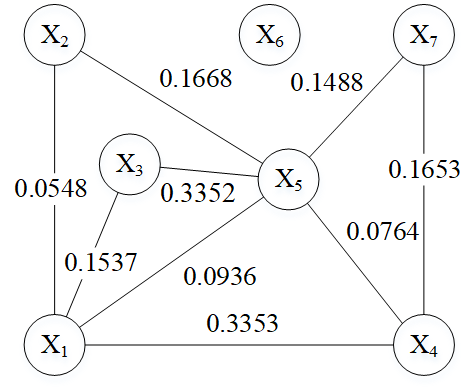
\includegraphics[width=3.0in]{./figures/chapter03/Figure1.png}
	\caption{属性关联依赖图}
	\label{Fig:attributes_dependence_graph}
\end{figure}

基于实验中的数据集,假设Marital-status($X_4$)为隐私敏感属性,则图$G$中与顶点$X_4$存在路径则构成隐私链,和$X_4$存在直接相连的边的属性构成关联属性组$\{X_1,X_5,X_7\}$。为和上文陈述保持一致,使用随机变量$X_h$表示隐私敏感属性$X_4$,$\bm{R}_h$表示和$X_4$存在关联的属性组。基于此利用本章中的信息熵方法量化关联属性的隐私泄露量。首先,基于样本观测数据统计关联属性组$\bm{R}_h$的联合概率分布,计算关联属性组联合信息熵$H(\bm{R}_h)=9.6712$ 。其次,计算敏感属性与关联属性组的联合信息熵$H(\bm{R}_hX_h) =10.8469$。由于原始数据集中的Marital-status为类别型数据,包含有七种不同的类别型取值,将其视为信源字母表空间,即域值。然后,利用敏感属性的概率分布计算隐私信源熵$H(X_h)=1.82$。进一步,基于熵与互信息的关系,计算得到互信息量$I(\bm{R}_h;X_h)=0.6442$,表示由属性关联导致的隐私敏感属性的信息泄露量。另外,条件熵$H(X_h|\bm{R}_h)$度量有关$X_h$仍具有的隐私不确定度,即$H(X_h)-I(\bm{R}_h;X_h)=1.1758$。

基于马尔可夫模型的隐私泄露链$\bm{R}_{h}\rightarrow X_{h}\rightarrow\hat{X}_{h}$关系,从信息论信道转移矩阵$Q(\hat{x}_h|x_h)$ 的角度构成马尔可夫状态转移矩阵。基于此,结合实验中的数据和数据处理不等式可得$I(\bm{R}_h;\hat{X}_h) \leq 0.6442$,量化隐私关联属性组泄露扰动数据信息量的上界。此外,依据公式\ref{eq:2.11}表述的费诺不等式,互信息隐私泄露量满足$I(X_h;\hat{X}_h)\geq 1.82-H(D)-D\log 6$,其中的$D={\rm Pr}\{X_h \neq \hat{X}_h\}$。

\begin{figure}[htbp]
	\centering
	\begin{minipage}[t]{0.48\textwidth}
		\centering
		\includegraphics[width=8cm]{./figures/chapter03/Figure2.png}
		\caption{差分隐私预算参数与失真度关系}
		\label{fig:epsilon_distortion}
	\end{minipage}
	\begin{minipage}[t]{0.48\textwidth}
		\centering
		\includegraphics[width=8cm]{./figures/chapter03/Figure3.png}
		\caption{互信息隐私泄露与失真度关系}
		\label{fig:mi_distortion}
	\end{minipage}
\end{figure}

针对隐私敏感属性$X_h$,考虑文献\mycite{alvim2011differential}中的对称离散信道情形,敏感属性在字母表空间中的每个符号正确传输的概率为$1-D$,误差概率为$\frac{D}{6}$,则此时的信道条件概率矩阵是$(7\times7)$阶的对称矩阵。 首先,针对这样的隐私机制,依据公式\ref{eq:epsilon_2.10}计算信道条件概率满足的差分隐私参数,图\ref{fig:epsilon_distortion}给出了差分隐私$\epsilon^{*}$与失真程度的对应变化关系。其次,对于已知的信源分布和特定的隐私机制,采用互信息公式\ref{eq:entropty_2.10} 计算互信息隐私泄露与期望失真度$D$之间的变化关系,图\ref{fig:mi_distortion}的结果展示了$D\rightarrow 0$ 时,互信息隐私泄露量$I(X_h;\hat{X}_h)\rightarrow H(X_h)$,由此验证分析了信息熵度量方法的有效性。



针对数据关联的隐私问题,文献\mycite{sankar2013utility}依据联合概率表达类别型属性之间具有的相关性,而对服从高斯分布的两相关联数值型随机变量$X$和$Y$,均值为$0$,方差为$\sigma_{X}^{2}$和$\sigma_{Y}^{2}$,采用皮尔逊相关系数法$\rho_{XY}=\mathbb{E}[XY]/(\sigma_X,\sigma_Y)$量化两随机变量之间的相关度。 然而,皮尔逊相关系数法适用于量化两两变量总体满足或接近高斯分布的线性相关性,对于非线性关系和非数值文本相关性的测量存在着不足。对比与上述采用的方法,本章中互信息的分析方法具有以下优势:

(1) 首先,本章基于Shannon通信模型,建立差分隐私通信模型。随后,研究面向多维属性关联关系数据集发布,提出的信息熵度量模型及方法针对更具体的差分隐私保护机制。

(2) 其次,采用互信息量化多维属性之间关联的相关度,是对数值型变量线性相关性分析的推广与延伸。互信息相关性分析克服了应用于混合数值型和类别型属性的局限性,能够有效的表达复杂的相关型关系。

(3) 最后,基于样本观测数据分析属性关联度,设定阈值门限过滤属性伪相关的影响,并据此生成属性的关联依赖图。然后,将属性集合划分为隐私关联属性组和隐私敏感属性,依据相关度的互信息隐私泄露度量相较于主观的划分更有科学理论。

\section{本章小结}
本章基于Shannon基本通信模型,给出差分隐私通信模型及其信道数学模型。以此通信模型为基本出发点,构建了一种属性关联、元组记录独立同分布的离散无记忆信源的$n$次扩展信源。在此基础上,引入信息熵、条件熵、互信息量、失真函数等概念给出了隐私信源熵、隐私熵与隐私泄露风险、数据效用的基本度量模型及方法。进一步,针对多维属性关联的隐私度量问题,基于信息熵提出了面向关联属性的差分隐私信息熵度量模型及方法。首先,利用互信息相关性分析方法解决关联属性相关度量化问题。随后,基于相关度给出关联属性的图表示。进一步,基于差分隐私的信道模型、属性关联图中隐私泄露关键路径,借助马尔可夫理论分析了关联属性导致敏感信息的隐私泄露量。最后,以真实数据集上的实验给出所提出的信息熵度量模型及方法的量化过程及结果。本章是研究差分隐私信息论度量的基础工作,为后续基于隐私信息度量研究权衡隐私与效用均衡优化模型以及隐私机制设计奠定基础。

 %CTL下遗忘的定义及语义属性 //CTL下的遗忘理论的定义及其语义属性
%\chapter{计算CTL下的遗忘:基于消解的方法}\label{chapter04}
{\em 本章针对隐私保护数据发布中隐私与效用的平衡问题,利用率失真理论研究了权衡隐私与数据效用的最优化隐私机制。首先,基于Shannon信息论通信模型与度量,在第\ref{chapter03}章的基础上,构建隐私-失真的最优化模型。然后,考虑关联知识对互信息隐私泄露的影响,借鉴条件互信息量,提出基于联合事件的互信息隐私度量,并修改率失真函数提出最小化隐私泄露的优化模型。最后,从凸优化问题求解的角度,分析拉格朗日构造泛函计算过程中存在的难题,由此基于率失真计算的交替最小化Blahut-Arimoto算法提出互信息隐私最优化模型的近似求解算法。分析与实验结果表明所提出的方法在满足数据效用约束的条件下,具有较小的互信息隐私泄露。}

\section{引言}
%\section{研究思路及框架}
当前,基于网络的信息服务已经应用到现实生活中的各个领域,包括医疗健康、社交网络、位置服务、推荐服务等。这些应用采集的基础数据中往往包含有诸如疾病、社会关系、位置、兴趣爱好等个人敏感信息。由于统计与科学发现的需要,应用服务中的数据应该被发布、共享。例如,医疗健康监测需要医院发布、共享患者电子病历数据。但是,敏感数据信息可能因数据标识或额外辅助数据而受到重识别和连接攻击导致隐私泄露\cite{sweeney2002k}。由于数据隐私问题,数据共享成为很多组织面临的困难问题。目前,解决数据发布、共享及应用中存在的隐私泄露问题,已经成为数据分析、数据挖掘和数据共享领域的一个重要研究内容。为解决上述问题,Dwork提出的差分隐私\cite{dwork2006differential,dwork2006calibrating,dwork2008differential,dwork2014algorithmic,dwork2015the}(Differential Privacy,DP)保护模型方法,迅速成为隐私保护研究的热点\cite{zhu2017differentially,zhangxiaojian2014,zhu2017differentially}。近年来,围绕差分隐私保护的隐私与数据效用权衡问题,学术研究基于不同的实现机制\cite{mcsherry2007mechanism,dwork2008differential,ghosh2012universally}提出了诸多的差分隐私方案。现有的工作依据模型假设的不同\cite{sarwate2014a},可以划分为非信息论和信息论方法两大类。本文将前者定义为经典差分隐私的研究范畴,后者利用信息论方法对差分隐私机制开展研究,逐渐成为一个新兴的研究方向。在信息论差分隐私模型中,以Shannon信息论\cite{shannon1948a} 为基本出发点,借鉴熵的量化工具,基于量化信息流\cite{smith2009on,alvim2011on,boreale2015quantitative,alvim2015on}(Quantitative Information Flow,QIF)的思想,考虑隐私保护模型中隐私泄露风险与数据效用的量化以及权衡问题,对于隐私与效用矛盾是行之有效的解决方法。


近年来,基于熵的信息度量在隐私保护中得到了诸多的应用\cite{issa2016an,liao2019tunable,Chatzikokolakis2008Anonymity,sankar2013utility},信息论方法与隐私保护结合的研究点现已逐渐引起国内学者的关注。如彭长根等\cite{peng2016}提出了隐私保护的信息熵模型、含敌手攻击的隐私信息熵模型和主观感受的加权隐私信息熵模型,并进一步提出了利用信息熵度量了隐私保护机制的信息泄露风险,为隐私保护效果评价提供了一种基于信息论的方法。此外,吴振强等\cite{zhenqiangwu2019}为度量社交网络的隐私保护效果,提出了网络结构熵的度量方法。更多地,信息论方法在差分隐私模型中用于隐私信息的量化,奠定了信息论差分隐私模型研究的基础\cite{mir2012information},同时建立了互信息隐私与差分隐私的关联\cite{cuff2016differential}。 对此方面,已存在不少的研究工作\cite{kalantari2018robust,alvim2011differential,wang2016on,sarwate2014a,wang2015a,du2015Fundamental,xiong2016randomized}利用信息论方法探讨最优化隐私保护机制问题\cite{kalantari2016optimal,kairouz2016extremal}。尽管如此,信息论方法对于差分隐私的研究还依然存在着诸多有待深入研究和思考的问题。例如,对于差分隐私数据发布中的隐私与失真函数\cite{wang2016on},在获得最小信息传输率的下界以及获得可达最小信息率时的最优化信道机制的问题等。

存在的差分隐私研究工作主要是针对数据独立情景,缺乏考虑数据关联和敌手拥有先验知识对隐私泄露的影响\cite{zhu2015correlated,li2019impact}。多数情况下,数据之间是存在关联的,并且由于数据关联可以辅助敌手识别出某些特定个体的隐私信息\cite{zhu2015correlated,yang2015bayesian}。例如,文献\mycite{zhu2015correlated}例举了医疗数据集中由于家庭住址相同对于流感疾病的影响,这是由于相同的属性信息辅助识别出其它个体疾病敏感信息的案例。又如,表\ref{tab:attributes_dependency_degree}所列出的属性之间的关联。这些关联的辅助数据信息被定义为隐私保护系统中敌手的背景知识,这意味着,如果敌手在一定的关联背景知识辅助下,则会获得更多的隐私信息量从而具有比较高的置信概率识别出个体隐私信息\cite{ningbowu2020}。 信息论方法中的条件互信息量表达了在给定条件下信宿获得有关信源的信息量。针对上述问题,条件互信息量能够度量敌手在拥有先验辅助背景知识条件下的互信息隐私泄露量。基于此,利用信息论方法在差分隐私中考虑敌手背景知识的影响,研究最小化互信息隐私泄露风险时的最优化信道机制问题就凸显重要。针对提出的这个问题,在本章中研究了最小化互信息隐私优化模型以及最优化隐私机制问题,提出了条件互信息隐私优化模型并设计了优化模型迭代算法。

围绕本章的研究内容,解决了以下几个关键问题,支撑了信息论差分隐私最优化模型与隐私机制的研究。首先,利用Shannon信息论方法,解决了差分隐私数据发布场景中权衡隐私与效用的最优化模型和含背景知识攻击下的最优化模型表达问题。其次,利用Lagrange 乘子法,解决了所提出优化模型的求解计算问题。最后,基于交替最小化算法,解决了本章中求解最优化隐私机制条件概率分布的算法问题。随着上述问题的解决,本章的研究工作实现了差分隐私数据发布中权衡隐私与效用的最优化隐私机制设计。对比目前存在的工作,本章的主要贡献总结为:

(1) 考虑差分隐私离线数据发布场景,结合差分隐私的离散无记忆信道模型,基于互信息的隐私风险度量和数据失真的效用度量提出了消息联合互信息隐私度量,建立了差分隐私数据发布与信息论通信模型之间的基本联系。

(2) 围绕信息率失真函数,将差分隐私数据发布场景中隐私泄露风险与数据效用平衡建模为带失真约束的最优化问题。在此基础上考虑了辅助背景知识攻击下的隐私与效用平衡问题,建立拥有辅助背景知识的差分隐私数据发布隐私与效用优化模型,并进一步考虑了求解差分隐私最小信息率的计算方法。

(3) 基于Blahut-Arimoto迭代最小化算法设计了计算最小化互信息隐私泄露的迭代算法,解决如何利用迭代求解算法计算差分隐私数据发布的最优信道条件转移概率,为差分隐私最优化机制设计提供了一种基于信息论的支撑。

%\begin{itemize}
%\item [(1)]考虑差分隐私离线数据发布场景,结合差分隐私的离散无记忆信道(DMC)模型,基于互信息的隐私风险度量和数据失真的效用度量提出了消息联合互信息隐私度量,建立了差分隐私数据发布与信息论通信模型之间的基本联系。
%
% \item [(2)]围绕信息率失真函数,将差分隐私数据发布场景中隐私泄露风险与数据效用平衡建模为带失真约束的最优化问题。在此基础上考虑了辅助背景知识攻击下的隐私与效用平衡问题,建立拥有辅助背景知识的差分隐私数据发布隐私与效用优化模型,并进一步考虑了求解差分隐私最小信息率的计算方法。
%
%\item [(3)]基于Blahut-Arimoto迭代最小化算法设计了计算最小化互信息隐私泄露的迭代算法,解决如何利用迭代求解算法计算差分隐私数据发布的最优信道条件转移概率,为差分隐私最优化机制设计提供了一种基于信息论的支撑。
%\end{itemize}

本章其余部分组织如下:首先,第\ref{chapter05-system-model}节介绍系统模型与研究问题,给出相关的定义和基本的符号表示。其次,第\ref{chapter05-optimal-model}节阐述本章针对权衡隐私与效用问题所提出的优化模型,并形式化的给出模型表述。第\ref{chapter05-optimazation-mechanism} 节对本章提出优化模型的求解方法及算法进行详细的阐述。第\ref{chapter04-experiment}节利用公开数据集对所提出的方法和算法进行实验分析。最后,第\ref{chapter04-conclusion}节对本章的主要工作进行总结。

\section{系统模型与问题提出}\label{chapter05-system-model}


本节给出本章的基本模型定义与符号表示,并阐述本章中的研究问题。

\subsection{数据模型}
通常,有关个体的信息可以表述为表\ref{tab:origin}具有的形式,即是由元组和属性组成的二维矩阵。本质上,这是一个关系数据模型,其中的数据是由元组信息组成的集合,每个元组是有关特定个体的一组属性描述信息。例如,表\ref{tab:origin}中元组由Age、Sex、Race等属性组成,又如,医疗数据中通常包含姓名、性别、出生日期、社保账号、疾病等信息。然而,在这样的数据集合中,通常有些属性值被认为是私有的敏感隐私信息(如表\ref{tab:origin}中的Marital-status、医疗数据中的疾病信息等),理应属于受保护的隐私数据。

基于关系代数理论,给出上述表达的关系模型表示。正式的,一个关系型数据集$\mathcal{D}$含有$n$个元组,其中的每个元组由$k$个属性组成,表示为$\mathcal{D}=\{d_1,\cdots,d_n\}$。以$k$属性组成的元组为单位,并假设其取值于一个域$\mathcal{X}$。其中的,$\mathcal{X}$表示所有$k$个属性域集合元素的笛卡尔积,基数$|\mathcal{X}|=M$,满足$M \geq 2$,代表数据域中离散的$M$个原子符号。对于任意的元组$d_i(1\leq i \leq n)$都是数据取值域全集$\mathcal{X}$的一个具体实例。由此,采用离散型随机变量$X$表示数据集,取值于有限域$\mathcal{X}$。对于任意两个数据集实例$x,x' \in \mathcal{X}$,汉明距离$d(x,x')$度量两个数据集实例之间不同元组的数目。如果汉明距离满足 $d(x,x')\leq 1$,则称$x,~x'$为相邻数据集,记作$x\sim x'$。基于以上的数据模型表示,差分隐私数据发布框架中,随机化隐私机制是一个算法$Q$,其接受原始数据库$\mathcal{D}$
输入,随机扰动输出噪声结果$Q(\mathcal{D})\rightarrow \mathbb{R}^{n}$\cite{dwork2014algorithmic}。由此,差分隐私保护机制的噪声扰动的随机化函数映射,与Shannon信息论中的噪声信道模型$\{X~Q(\hat{X}|X)~\hat{X}\}$\cite{xiong2016randomized,alvim2011differential}不谋而合。以此为基本的出发点,本章\ref{chapter05-achieve-channel}节从信息论的角度给出具体的阐述与分析。

\subsection{信道模型}\label{chapter05-achieve-channel}

本节在\ref{sec:communication_model_of_dp}节介绍的差分隐私通信模型的基础上,给出更详细的信道模型细节描述。首先,在差分隐私的离线数据发布应用场景中,差分隐私随机化机制接受原始数据输入,概率性映射输出原始数据的近似净化副本。差分隐私机制与Shannon通信系统在数据处理流程方面具有相似之处。基于此,可以从Shannon信息论的角度,将差分隐私机制表述为从字母表$\mathcal{X}$到再生字母表$\mathcal{\hat{X}}$的条件概率映射。本节以此为基本的出发点,将对数据集的差分隐私保护建模为信息论信道模型。为方便理解,首先给出以下简单示例。对于``是''和``否''问题类型的二进制数据集$\mathcal{D}=\{0,1\}^{n}$,$p_x(0)$和$p_x(1)$分别表示概率分布,$q_{\hat{X}|X}(\hat{x}|x),(x,\hat{x}\in \{0,1\})$表达随机化隐私机制$X\xrightarrow{Q} \hat{X}$,本质上该表达是信息论二元对称信道(Binary Symmetric Channel,BSC)模型。除此之外,对于如表\ref{tab:origin}中Marital-status、医疗数据中疾病信息等离散类别型数据,都可以使用条件概率$q(\cdot|\cdot)$形式表示为两个有限离散集合之间的概率性映射关系。对此,本章中延承差分隐私基本通信模型开展本章隐私机制的研究。

上述分析奠定了信道模型的理论基础,本节中结合差分隐私离线数据发布的数据混淆原理,将其建模为原始数据信源$X$到混淆、扰动数据信宿$\hat{X}$之间的点对点通信模型$\{X~Q(\hat{X}|X)~\hat{X}\}$,扰动输出仅统计依赖于原始输入的离散无记忆信道(Discrete Memoryless Channel,DMC)模型。正式的,$\mathcal{X}$和$\mathcal{\hat{X}}$分别表示有限的离散字母表集合,随机化函数映射$Q:\mathcal{X}\rightarrow\hat{\mathcal{X}}$表示为条件概率$q(\hat{x}|x)$矩阵形式。为了捕捉类别型数据的语义完整性,不失一般性考虑$\mathcal{X}=\hat{\mathcal{X}}$的情况,对字母表$\mathcal{X}$中原子符号序列化表示$1,2,\cdots,M$,则有
\begin{equation}\label{Eq:MRR_5.2.2}\nonumber
	q(\hat{x}|x)=\begin{pmatrix}
		q_{(1|1)}& q_{(2|1)}&\cdots &q_{(j|1)}&\cdots & q_{(M|1)}\\
		q_{(1|2)}& q_{(2|2)}&\cdots &q_{(j|2)}&\cdots & q_{(M|2)}\\
		\vdots & \vdots & \vdots &\vdots &\vdots & \vdots \\
		q_{(1|i)}  & q_{(2|i)} &\cdots & q_{(j|i)}& \cdots &q_{(M|i)}\\
		\vdots & \vdots & \vdots &\vdots &\vdots & \vdots \\
		q_{(1|M)}& q_{(2|M)}&\cdots &q_{(j|M)}&\cdots & q_{(M|M)}
	\end{pmatrix}
\end{equation}
基于上述信道模型的条件概率$q(\hat{x}|x)$表示,信道概率分布的统计性质反映了差分隐私的随机化特性。由此,结合本章上下文给出以下差分隐私的定义。
\begin{definition}\textup{\cite{alvim2011differential,wang2016on}}\label{def:chapter05-dp}对于$\epsilon \in \mathbb{R}^{+}$,一个离散无记忆信道模型$\mathcal{Q}:\mathcal{X}\times \mathcal{\hat{X}}\rightarrow \mathbb{R}^{+} $ 满足$\epsilon$-差分隐私($\epsilon$-DP),当且仅当对所有的$x$,$x'\in \mathcal{X}$,汉明$d(x,x')\leq 1$和$\hat{x}\in \mathcal{\hat{X}}$,信道条件概率$q(\cdot|\cdot)$满足$\epsilon$-概率不可区分性
	\begin{equation}
		q(\hat{x}|x)\leq \exp (\epsilon) \times q(\hat{x}|x')
	\end{equation}
\end{definition}

\begin{remark}
{\em 定义\textup{\ref{def:chapter05-dp}}的表述依赖于信道模型条件概率分布$q(\hat{x}|x)$,反映了信道统计特性。由此,差分隐私的隐私保护水平定义为
\begin{equation}\label{eq:chapter05-epsilon}
	\epsilon^{*}\triangleq \inf \left(\epsilon: \ln \frac{q(\hat{x}|x)}{q(\hat{x}|x')}\right),x,x'\in \mathcal{X}\text{和}\hat{x}\in \mathcal{\hat{X}}
\end{equation}
}
\end{remark}
信道模型的信息传输率$R$和期望失真$\mathbb{E}\left[d(X,\hat{X})\right]$与信道条件概率$q(\hat{x}|x)$和先验分布$p(x)$密切相关。信息论差分隐私模型中考虑数据先验分布$p(x)$的影响,基于隐私与失真关系约束数据质量损失的$(\epsilon,\delta)$可达信道集合可以定义为

%噪声信道条件概率与信息传输率$R$和失真紧密联系,从满足失真约束的角度,可以定义$(\epsilon,\delta)$可达信道集合。
\begin{definition}\label{def:achievechannel}对于给定的数据分布$p(x)$和失真函数$d(x,\hat{x})$,期望失真$\mathbb{E}\left[d(X,\hat{X})\right]$不超过给定的失真门限$\delta$的所有$\epsilon$-差分隐私信道$q(\hat{x}|x)$称为$(\epsilon,\delta)$可达信道集合,则有
	\begin{equation}
		(\epsilon,\delta)\stackrel{\text{def}}{=} \left\{q(\hat{x}|x):\sum_{x,\hat{x}}p(x)q(\hat{x}|x)d(x,\hat{x})\leq \delta\right\}
	\end{equation}
\end{definition}

基于上述定义\ref{def:achievechannel},本章中的研究是在满足差分隐私与给定失真度的$(\epsilon,\delta)$可达信道中寻找概率分布$q(\hat{x}|x)$。 由期望失真公式\ref{eq:chapter03-ED}易知可行集是超平面的闭半空间,并且半空间是凸的\cite{boyd2004convex},封闭的,凸的且满足$\sum_{\hat{x}}q(\hat{x}|x)=1, q(\hat{x}|x)\geq 0$。由此,利用凸集合交集的保凸运算规则,$(\epsilon,\delta)$可达信道集合依然保持凸性。此外,文献\mycite{xiong2016randomized}中已经从下水平集的角度证明了$\epsilon$参数的计算函数是拟凸函数。基于此,本章中的研究是在凸可行集中计算最优分布$q(\hat{x}|x)$优化问题。



\subsection{问题提出}\label{chapter05-problem-statement}

本小节中引入隐私泄露与数据效用的信息论度量方法,然后给出本章研究问题的详细描述。首先,差分隐私的语义安全考虑了敌手有关数据的先验分布与后验概率分布的距离,据此量化隐私泄露。Kullback-Leibler (KL)散度是度量两个概率分布之间距离的有效工具\cite{cover2006elements}。针对此,定义敌手后验概率分布$p(x|\hat{x})$ 与先验分布$p(x)$之间的相对熵距离度量平均情况下的隐私泄露量。事实上,期望形式的相对熵度量等效于互信息量$I(X;\hat{X})$\cite{calmon2012privacy},

\begin{equation}\label{chapter05-privacy-metrics}
	I(X;\hat{X})=\mathbb{E}_{\hat{X}}D_{KL}\left(p(x|\hat{x})\parallel p(x)\right)
\end{equation}
其中, $D_{KL}(\cdot \parallel \cdot)$是相对熵距离函数。

%互信息度量近似合成数据$\hat{X}$包含原始数据$X$的信息量。因此,可以定义互信息量度量差分隐私离线数据发布框架中的隐私泄露风险。此外,互信息$I(X;\hat{X})=H(X)-H(X|\hat{X})$,依据熵与互信息的关系,互信息$I(X;\hat{X})$刻画观测到$\hat{X}$后有关随机变量$X$不确定度的减少量,条件熵$H(X|\hat{X})$表述随机变量仍具有的不确定度。对于固定信源概率分布,$H(X)$固定。由此,隐私泄露风险度量的互信息与条件熵可视为等价可替换的量化方法\cite{zhang2019online}。
\begin{remark}{\em
在本章中我们采用上述公式}\ref{chapter05-privacy-metrics}{\em 的形式度量混淆合成数据$\hat{X}$包含原始数据$X$的隐私泄露量。平均互信息量是数据先验分布$p(x)$和信道条件概率分布$q(\hat{x}|x)$的函数,是关于$p(x)$的凸函数,$q(\hat{x}|x)$的凹函数。}
\end{remark}
%\subsection{效用度量}

其次,为表达混淆输出数据的质量损失,采用汉明距离$d(x,\hat{x})$定义$X$与$\hat{X}$之间的期望汉明失真
\begin{equation}\label{eq:chapter05-distortion}
	\mathbb{E}\left[d\left(X,\hat{X}\right)\right]=\sum_{x}\sum_{\hat{x}}p(x)q(\hat{x}|x)d(x,\hat{x})
\end{equation}
度量平均的失真程度。由上式\ref{eq:chapter05-distortion}可知,$	\mathbb{E}\left[d\left(X,\hat{X}\right)\right]$是有关$p(x)$、$q(\hat{x}|x)$和失真测量~$d(x,\hat{x})$~的函数。本章中利用期望汉明失真度量就是同时考虑了数据分布和信道概率分布的影响。

基于上述分析及符号表示,本章中的基础研究可以表述为差分隐私数据发布中约束数据质量损失$\delta$的条件下最小化隐私泄露的隐私机制条件概率分布求解问题,$\min_{q(\hat{x}|x):\sum_{x}\sum_{\hat{x}}p(x)q(\hat{x}|x)d(x,\hat{x})\leq \delta}I(X;\hat{X})$。其次,针对含有关联背景知识$Z$的敌手模型,研究给定数据质量损失门限,差分隐私最优的概率分布函数设计问题,$\min_{q(\hat{x},z|x):\sum_{x}\sum_{\hat{x}}\sum_{z}p(x)q(\hat{x},z|x)d(x,\hat{x})\leq  \delta}I(X;\hat{X},Z)$。围绕上述问题,本章开展了权衡隐私与效用的优化模型与算法研究。接下来,\ref{chapter05-optimal-model}节阐述具体的优化模型,\ref{chapter05-optimazation-mechanism}节给出模型计算及算法的伪代码描述。

\section{隐私与效用的优化模型}\label{chapter05-optimal-model}
本节中介绍本章针对权衡隐私与效用问题所提出的优化模型。首先\ref{subsec:chapter05-yjsl}小节给出一个总体的研究方案框架,然后,分别在\ref{subsec:chapter05-mi-optimazation}小节介绍互信息隐私优化模型,\ref{subsec:chapter-05-conditional-mioptimization}小节阐述数据关联的条件互信息优化模型。

\subsection{研究方案概述}\label{subsec:chapter05-yjsl}
本章基于信息论的方法,从优化的角度研究权衡隐私泄露与数据效用的互信息隐私最优化问题。为了更好地阐述本章的研究工作,首先给出研究的框架示意图,如下图\ref{Fig:chapter05-1}所示。
\begin{figure}[htbp]
	\centering
	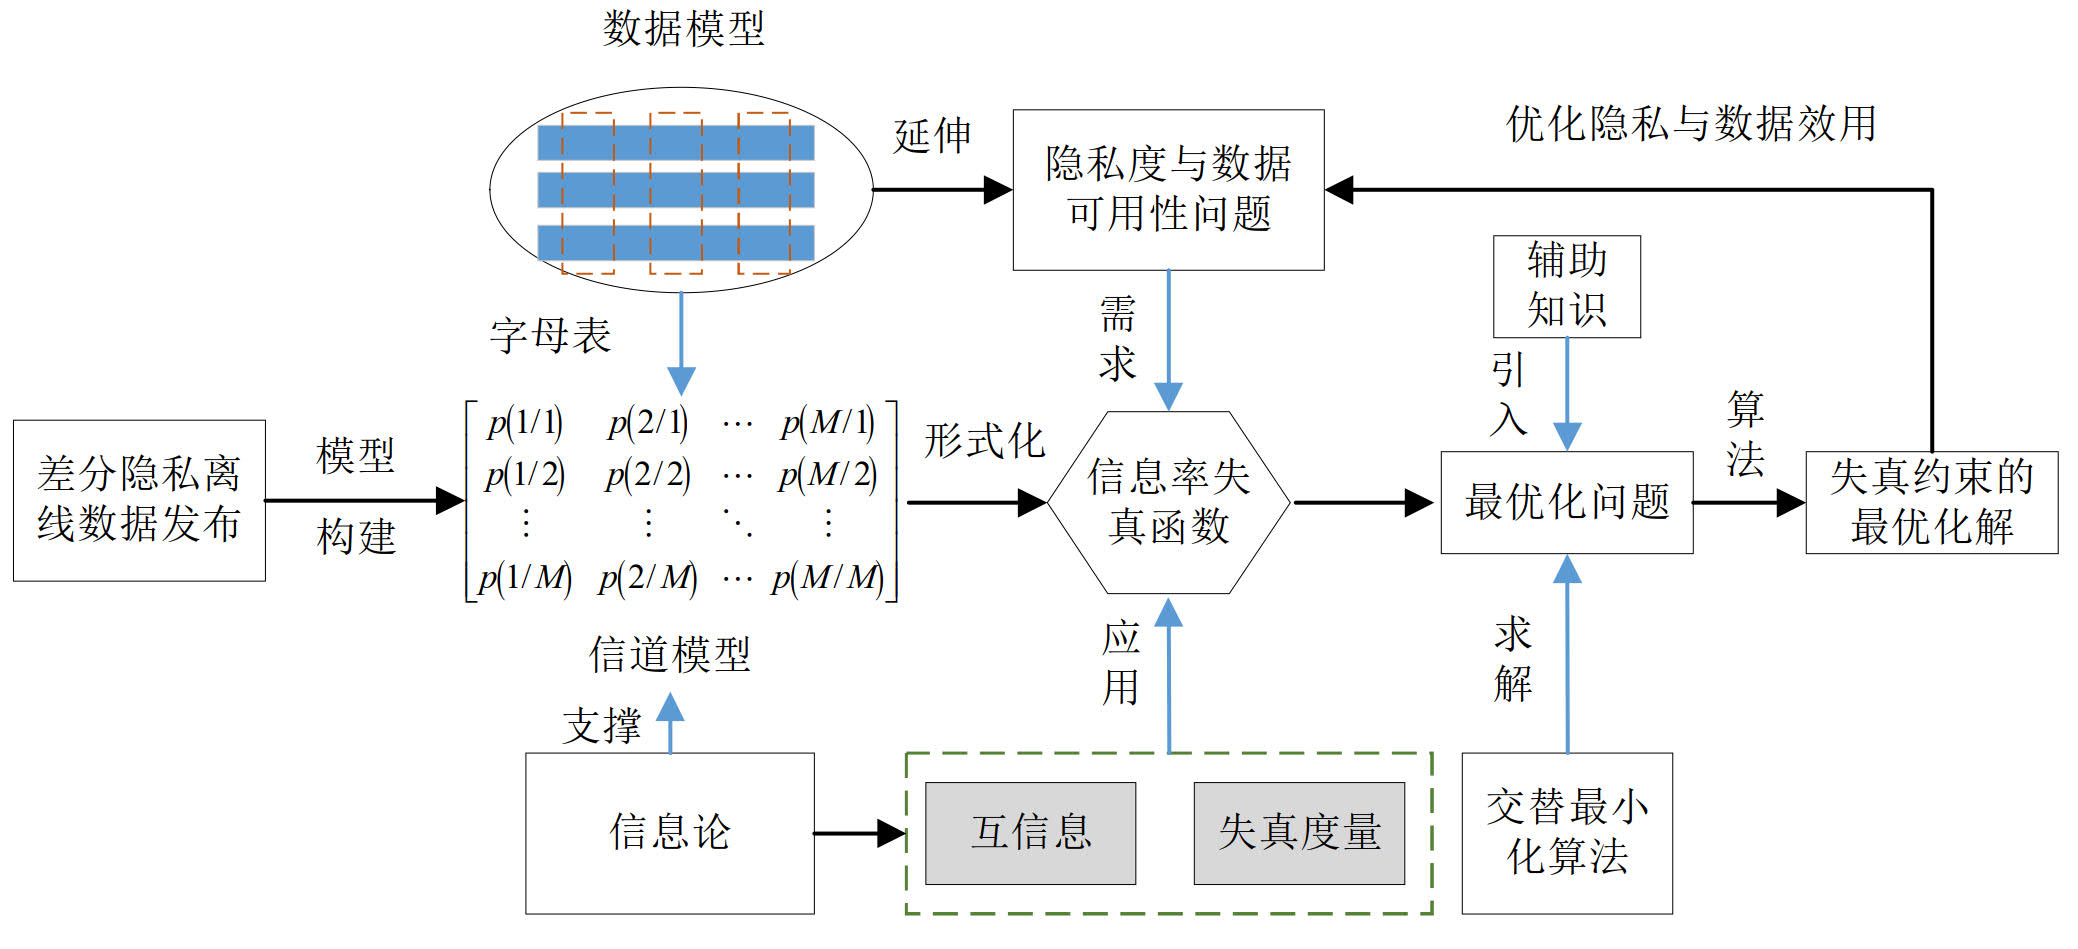
\includegraphics[width=5.0in]{chapter04/Figure4-1.jpg}
	\caption{权衡隐私与效用的差分隐私优化机制研究框架}
	\label{Fig:chapter05-1}
\end{figure}

在图\ref{Fig:chapter05-1}中,以差分隐私离线数据发布应用场景为立意的出发点,使用信息论、优化理论的方法解决数据发布中权衡隐私泄露与数据效用问题为研究目标。以下具体的介绍本章的研究思路:首先,通过分析差分隐私离线数据发布中原始数据扰动输出数据副本的处理流程,以数据模型、信道模型为基础,构建差分隐私信道模型。随后,从通信的角度给出本章信道模型的数学表达。以此为基础,针对隐私与效用的权衡问题,在熵与失真的度量基础上,将权衡隐私与效用的问题形式化为限失真约束条件下的最小化隐私信息泄露问题,给出互信息隐私优化模型,与著名的信息率失真函数具有相似的表述形式。其次,在差分隐私通信模型中引入含辅助背景知识攻击的敌手模型,将敌手拥有背景知识条件下的隐私与效用的权衡问题形式化为多约束条件的一个凸优化问题,给出条件互信息优化模型。最后,针对上述优化模型,研究模型的计算与算法求解问题。

\subsection{互信息隐私优化模型}\label{subsec:chapter05-mi-optimazation}
基于信息熵的度量模型及方法,互信息量度量差分隐私数据发布的隐私泄露,期望失真量化发布数据与原始数据的失真程度,也即是数据的可用性。直观上理解,差分隐私数据发布中的隐私泄露与数据效用是极大极小的矛盾问题。依据隐私保护中的隐私与效用原则\cite{sankar2013utility},权衡隐私与数据效用属于最优性均衡解决的问题。以此为理论的出发点,在限定数据可用性约束的前提下,利用隐私-失真函数形式化表述权衡问题为如下的优化模型$1$的形式。

\textbf{模型1:}差分隐私信道模型$\mathcal{Q}:\mathcal{X}\times \mathcal{\hat{X}}\rightarrow \mathbb{R}^{+}$获得可达的最小互信息隐私泄露量,当且仅当对于给定的数据分布$p(x)$,失真函数$d(x,\hat{x})$和数据质量约束$\mathbb{E}[d(X,\hat{X})]\leq \delta$,信道概率分布$q(\hat{x}|x)$是下述凸优化模型的最优解。
\begin{alignat}{2}
	R(\delta) & =\min_{q(\hat{x}|x)}I(X;\hat{X}) \nonumber \\
	\mbox{subject to} \quad
	& \sum_{x}\sum_{\hat{x}}p(x)q(\hat{x}|x)d(x,\hat{x})\leq  \delta \label{eq:chapter04-4-6}\\
	& \sum_{\hat{x}}q(\hat{x}|x)=1 \\
	& q(\hat{x}|x) \geq 0\label{eq:chapter04-4-8}
\end{alignat}
其中的$I(X;\hat{X})$和公式\ref{eq:chapter04-4-6}$\sim$\ref{eq:chapter04-4-8}分别是优化模型$1$的优化目标函数和约束条件,描述满足约束条件的$q(\hat{x}|x)$中寻找极小化$I(X;\hat{X})$的问题。

上述的优化模型$1$从隐私-失真的角度\cite{wang2016on}给出了权衡隐私与数据效用的基本优化模型,最小化信息率$R(\delta)$的形式化表述和Shannon信息论率失真函数\cite{cover2006elements}具有相同的表达形式,是关于信道条件概率分布$q(\hat{x}|x)$的最小值问题。在隐私保护中,最优化模型$1$在满足给定数据质量损失门限的前提条件下,求解最小化互信息隐私泄露的数据混淆机制,即信道条件概率分布。对此,文献\mycite{mir2012information,wang2016on}中已经给出了获得最优率失真的隐私机制依然提供一个确定等级差分隐私保护的结论。借用这个结论,通过上述模型$1$获得的信道概率满足$(\epsilon,\delta)$可达信道。
\subsection{条件互信息优化模型}\label{subsec:chapter-05-conditional-mioptimization}

上述优化模型$1$刻画了隐私与失真函数的关系,在隐私保护中具有广泛的应用\cite{wang2016on,sarwate2014a,mir2012information}。但是,上述模型中的隐私和失真函数没有考虑差分隐私离线数据发布场景中关联辅助背景知识对互信息隐私泄露的影响。实际应用中,由于隐私攻击者可能通过其它途径获取隐私关联数据,从而导致隐私泄露问题。本章中使用随机变量$Z$表示辅助的背景知识,并考虑由$Z$辅助识别的互信息隐私泄露问题。具体地说,依据隐私保护数据发布者和隐私攻击者对背景知识$Z$
的了解程度,将含背景知识的优化问题划分为如下的两种情形进行考虑:

%(1) 辅助背景知识$Z$是隐私保护数据发布者和隐私攻击者都知道的共同知识。在这种情况下,互信息的隐私度量$I(X;\hat{X})$改变为给定$Z$的条件下$X$和$\hat{X}$之间的条件互信息量$I(X;\hat{X}|Z)$。针对此,上述优化模型$1$中的最小化目标函数改变为求解变量$q(\hat{x}|x,z)$,使得条件互信息$I(X;\hat{X}|Z)$获得最小值。
%
%(2) 辅助背景知识$Z$是隐私攻击者可通过其它途径获得的外部关联数据,刻画了攻击者的能力。但是,数据发布者拥有一定有关辅助背景知识的统计信息,而未能精准的获得$Z$的具体数据细节。在这样的情形下,互信息的隐私度量$I(X;\hat{X})$改变为$X$和联合变量$\hat{X},Z$之间的互信息量$I(X;\hat{X},Z)$。针对此,上述优化模型$1$的最小化目标函数改变为求解条件概率$q(\hat{x},z|x)$使得$I(X;\hat{X},Z)$最小化。
\begin{itemize}[leftmargin=2em]
\item [(1)]辅助背景知识$Z$是隐私保护数据发布者和隐私攻击者都知道的共同知识。在这种情况下,互信息的隐私度量$I(X;\hat{X})$改变为给定$Z$的条件下$X$和$\hat{X}$之间的条件互信息量$I(X;\hat{X}|Z)$。针对此,上述优化模型$1$中的最小化目标函数改变为求解变量$q(\hat{x}|x,z)$,使得条件互信息$I(X;\hat{X}|Z)$获得最小值。

\item [(2)]辅助背景知识$Z$是隐私攻击者可通过其它途径获得的外部关联数据,刻画了攻击者的能力。但是,数据发布者拥有一定有关辅助背景知识的统计信息,而未能精准的获得$Z$的具体数据细节。在这样的情形下,互信息的隐私度量$I(X;\hat{X})$改变为$X$和联合变量$\hat{X},Z$之间的互信息量$I(X;\hat{X},Z)$。针对此,上述优化模型$1$的最小化目标函数改变为求解条件概率$q(\hat{x},z|x)$使得$I(X;\hat{X},Z)$最小化。
\end{itemize}

结合差分隐私离线数据发布应用场景中原始数据$X$到扰动数据$\hat{X}$之间的数据混淆过程,所表达出的隐私通信模型$X\xrightarrow{Q}\hat{X}$。考虑隐私攻击者可通过观察$\hat{X}$后,关联拥有的可用背景知识$Z$对原始数据$X$中的隐私信息进行推断攻击的敌手模型。本章中把隐私攻击者可以得到的背景知识$Z$考虑为仅攻击者拥有的知识。数据发布的混淆扰动过程表述为如图~\ref{Fig:chapter05-2}所示的隐私通信模型。
\begin{figure}[htbp]
	\centering
	\includegraphics[width=5.0in]{chapter04/Figure2.png}
	\caption{含有背景知识攻击的差分隐私通信模型}
	\label{Fig:chapter05-2}
\end{figure}

为了更好的说明上图\ref{Fig:chapter05-2}中隐私攻击者具有关联辅助背景知识$Z$对互信息隐私泄露风险的影响,首先从理论上给出下述定理\ref{theorem:5.1}。
\begin{theorem} \label{theorem:5.1}随机变量$X$与$\hat{X},Z$的联合互信息量$I(X;\hat{X},Z)$不小于互信息$I(X;\hat{X})$。
\end{theorem}
\textbf{证明定理\ref{theorem:5.1}:}由随机变量$X$和$X,Z$联合的互信息量定义,则有
\begin{alignat}{2}
	I(X;\hat{X},Z) & =\sum_{x}\sum_{\hat{x}}\sum_{z}p(x,\hat{x},z)\log \frac{q(x|\hat{x},z)}{p(x)} \\
	 & = \sum_{x}\sum_{\hat{x}}\sum_{z}p(x,\hat{x},z)\log \left( \frac {q(x|\hat{x},z)}{q(x|\hat{x})}\cdot \frac{q(x|\hat{x})}{p(x)} \right)\\
	 & = \sum_{x}\sum_{\hat{x}}p(x,\hat{x})\log \frac{q(x|\hat{x})}{p(x)} \nonumber \\
	 & +\sum_{x}\sum_{\hat{x}}\sum_{z}p(x,\hat{x},z)\log \frac{q(x|\hat{x},z)}{q(x|\hat{x})}\\
	 & = I(X;\hat{X})+I(X;Z|\hat{X})\\
	 & \geq I(X;\hat{X})
\end{alignat}
易知,$I(X;\hat{X},Z)$是互信息$I(X;\hat{X})$和条件互信息$I(X;Z|\hat{X})$之和。因为平均互信息的非负性,则有结论成立。

基于上述互信息隐私泄露量的分析,拥有背景知识$Z$相对于$I(X;\hat{X})$可增加隐私泄露量。以此为基础,接下来将差分隐私数据发布中隐私攻击者拥有背景知识$Z$的最小化互信息隐私泄露问题定义为

\begin{definition}对于给定$X$的失真函数$d(x,\hat{x})$,差分隐私信道模型$\mathcal{Q}:\mathcal{X}\times \mathcal{\hat{X}}\rightarrow \mathbb{R}^{+}$,在满足$\mathbb{E}[d(X,\hat{X})]\leq \delta$的约束下,隐私信道获得的最小互信息隐私泄露量为信息率$R_{z}(\delta)$。其中,$R_{z}(\delta)$为下述最优化模型$2$的最优值。
\end{definition}

\textbf{模型2:}对于数据$X$的失真函数$d(x,\hat{x})$,在$Z$的条件下,数据质量满足限失真门限$\delta$的约束,条件概率$q(\hat{x},z|x)$是获得最小化互信息隐私泄露$R_{z}(\delta)$ 的最优点,即是下述优化问题的最优解。
\begin{alignat}{2}%\label{eq:chapter05-model2}
	R_{z}(\delta) & =\min_{q(\hat{x},z|x)}I(X;\hat{X},Z) \nonumber \\
	\mbox{subject to} \quad
	& \sum_{x}\sum_{\hat{x}}\sum_{z}p(x)q(\hat{x},z|x)d(x,\hat{x})\leq  \delta \label{eq:chapter04-14}\\
	& \sum_{\hat{x}}\sum_{z}q(\hat{x},z|x)=1\\
	& q(\hat{x},z|x) \geq 0\label{eq:chapter04-16}
\end{alignat}
其中$I(X;\hat{X},Z)=\sum_{x,\hat{x},z}p(x,\hat{x},z)\log \frac{q(\hat{x},z|x)}{p(\hat{x},z)}$和公式\ref{eq:chapter04-14}$\sim$\ref{eq:chapter04-16}分别为目标函数和约束条件。

上述最优化模型$2$是互信息隐私泄露$I(X;\hat{X},Z)$关于条件概率分布$q(\hat{x},z|x)$的最小值求解问题。换句话表述,上述优化模型$2$的最优解$q(\hat{x},z|x)$就是在数据质量损失约束条件下,使得互信息量$I(X;\hat{X},Z)$获得极小值。

\section{差分隐私数据发布机制与优化}\label{chapter05-optimazation-mechanism}

本节中针对上述优化模型$2$,利用Lagrange对偶函数的方法对权衡隐私与效用的优化模型进行求解,给出KKT条件的参量表达式。然后,针对直接计算最优条件概率分布的困难性问题,基于Blahut-Arimoto算法给出了差分隐私数据发布场景中计算最优信道条件概率分布的迭代算法。

\subsection{优化模型最优解}

借鉴率失真函数的求解方法,最优化模型$2$是满足期望失真约束和条件概率分布约束条件下,有关凸目标函数的一个标准最小化问题。对其利用Lagrange乘子法进行求解,首先构造以下泛函$L(q)$
\begin{alignat}{2}
	L(q) & =\sum_{x}\sum_{\hat{x},z}q(\hat{x},z|x)\log \frac{q(\hat{x},z|x)}{q(\hat{x},z)} \nonumber \\
	  & + \lambda \sum_{x}\sum_{\hat{x},z}p(x)q(\hat{x},z|x)d(x,\hat{x}) \\
	& +\sum_{x}\nu (x)\sum_{\hat{x},z}q(\hat{x},z|x) \nonumber
\end{alignat}

然后,对构造的$L(q)$关于$q(\hat{x},z|x)$求偏导数,并令$\frac{\partial L(q)}{\partial q(\hat{x},z|x)}=0$得到如下含有拉格朗日乘子参数$\lambda$的表达式
\begin{alignat}{2}
	\frac{\partial L(q)}{\partial q(\hat{x},z|x)} & =p(x)\log \frac{q(\hat{x},z|x)}{q(\hat{x},z)}+p(x)
	-\sum_{x'}p(x')q(\hat{x},z|x')\frac{1}{q(\hat{x},z)}p(x) \nonumber \\
	 & + \lambda p(x)d(x,\hat{x}) \\
	& +\nu (x) \nonumber \\
	& = 0 \nonumber
\end{alignat}
由于先验概率分布$p(x)\geq 0$,利用KKT条件可以计算得到使得互信息最小化的条件概率$q(\hat{x},z|x)$参量表达式
\begin{equation}\label{eq:chapter05-pdf}
	q(\hat{x},z|x)=\frac{q(\hat{x},z)e^{-\lambda d(x,\hat{x})}}{\sum_{\hat{x},z}q(\hat{x},z)e^{-\lambda d(x,\hat{x})}}
\end{equation}

然而,通过联合方程组的方式直接解出最优输出分布仍然比较困难。针对这个计算的困难问题,Blahut和Arimoto\cite{arimoto1972an,blahut1972computation}提出了计算率失真函数的迭代求解算法,该算法是两个概率分布凸集之间计算最小相对熵距离的一种特殊情况\cite{cover2006elements}。已经证明算法在两个概率分布凸集之间交替最小化相对熵距离的计算过程中存在一个极限,收敛到相对熵距离最小值。基于此,求解率失真$R(\delta)$需要将率失真函数改写为两个集合之间相对熵距离最小化的形式。为了将其改进应用到优化模型$2$的求解计算中,以下给出计算的预处理过程。

\subsection{交替最小化算法}
对于两个给定凸集$A$和$B$以及欧几里得范数距离,目标是计算集合$A$和$B$之间的最小欧氏距离。利用交替最小化的思想,首先,选择任意的$a \in A$ ,计算$b \in B$满足~$\min \parallel a-b\parallel_{2}$。然后固定~$b$,在集合$A$中计算欧式距离和$b$最近的元素。重复上述计算过程,随着重复次数增加,特定的距离度量收敛于两个集合的最小值\cite{cover2006elements}。特别地,如果上述是在两个概率分布集合$A$和$B$之间的相对熵(Kullback-Leibler,KL) 距离度量中,最小化距离的算法将收敛到$A$和$B$之间的最小相对熵\cite{csiszar1984information}。

本章中,基于上述最小化算法的交替计算过程对提出的优化模型进行求解。首先,需要将其改写为相对熵距离在两个概率分布集合之间双重最小化的形式。为此,给出以下引理\ref{lemma:chapter05-1}。
\begin{lemma}\label{lemma:chapter05-1}设$p(x)q(\hat{x},z|x)$是给定的联合分布,使得最小化相对熵$D(p(x)q(\hat{x},z|x)\parallel p(x)r(\hat{x},z))$~的分布$r(\hat{x},z)$是对应于条件概率$q(\hat{x},z|x)$的边缘分布$r^*(\hat{x},z)$,也即是
	\begin{equation}\label{lemma5.1}
		D_{KL}(p(x)q(\hat{x},z|x)\parallel p(x)r^*(\hat{x},z))=\min_{r(\hat{x},z)}D_{KL}(p(x)q(\hat{x},z|x)\parallel p(x)r(\hat{x},z))
	\end{equation}
	其中,$r^*(\hat{x},z)=\sum_{x}p(x)q(\hat{x},z|x)$。
\end{lemma}
\textbf{证明引理\ref{lemma:chapter05-1}:}根据相对熵$D_{KL}(\cdot||\cdot)$的定义,构造
\begin{alignat}{2}
	D_{KL}\left( p(x)q(\hat{x},z|x)\parallel p(x)r(\hat{x},z)\right)
	 & -D_{KL}\left(p(x)q(\hat{x},z|x)\parallel p(x)r^{*}(\hat{x},z)\right) \\
	 & =\sum_{x,\hat{x},z}p(x)q(\hat{x},z|x)\log \frac{p(x)q(\hat{x},z|x)}{p(x)r(\hat{x},z)}\\
	 & - \sum_{x,\hat{x},z}p(x)q(\hat{x},z|x)\log \frac{r^*(\hat{x},z)}{r(x,z)}\\
	 & = \sum_{x}\sum_{\hat{x}}p(x,\hat{x})\log \frac{q(x|\hat{x})}{p(x)} \nonumber \\
	 &=\sum_{\hat{x},z}r^*(\hat{x},z)\log \frac{r^*(\hat{x},z)}{r(x,z)}\\
	 & =D_{KL}\left(r^*(\hat{x},z)\parallel r(\hat{x},z)\right)
\end{alignat}
由于相对熵的非负性质,则有$D_{KL}\left(r^*(\hat{x},z)\parallel r(\hat{x},z)\right)\geq 0$的结论。当且仅当,$r^*(\hat{x},z)= r(\hat{x},z)$ 时等号成立。

基于引理\ref{lemma:chapter05-1}和$I(X;\hat{X},Z)=\sum_{x}\sum_{\hat{x}}\sum_{z}p(x,\hat{x},z)\log \frac{q(\hat{x},z|x)}{p(\hat{x},z)}$的计算公式,可以将上述优化模型$2$中的最优化目标函数$I(X;\hat{X},Z)$表述为一个具有相对熵距离的双重最小化问题的形式,则有
\begin{alignat}{2}
& \min_{q(\hat{x},z|x):\sum_{x,\hat{x},z}p(x)q(\hat{x},z|x)d(x,\hat{x})\leq  \delta}\sum_{x,\hat{x},z} p(x,\hat{x},z)\log \frac{q(\hat{x},z|x)}{p(\hat{x},z)}\\
=\min_{r(\hat{x},z)}&\min_{q(\hat{x},z|x):\sum_{x,\hat{x},z}p(x)q(\hat{x},z|x)d(x,\hat{x})\leq  \delta}\sum_{x,\hat{x},z}p(x)q(\hat{x},z|x)\log \frac{q(\hat{x},z|x)}{r(\hat{x},z)}\label{eq:chapter05-double}
\end{alignat}

针对上式~\ref{eq:chapter05-double}中的双重最小化问题,利用交替最小化算法进行计算近似最优解。如果集合$A$为边际分布$p(x)$满足期望失真门限的所有联合概率分布 $p(x,\hat{x},z)$的集合,$B$为乘积分布$p(x)r(\hat{x},z)$构成的集合,则对于任意的分布$r(\hat{x},z)$,上述公式\ref{eq:chapter05-double}中的双重最小化可以表述为如下公式\ref{eq:chapter04-1-28}的形式,

\begin{equation}\label{eq:chapter04-1-28}
	\min_{q(\hat{x},z|x):\sum_{x,\hat{x},z}p(x)q(\hat{x},z|x)d(x,\hat{x})\leq  \delta } I(X;\hat{X},Z)=\min_{q \in B}\min_{p \in A} D_{KL}(p\parallel q)
\end{equation}

基于上述方法将优化模型$2$中的问题转变为了两个概率分布集合之间计算最小相对熵距离的双重最小化问题。然后,借鉴计算率失真函数的交替最小化算法\cite{csiszar1984information,csiszar1974on},设计本章中对优化模型$2$求解的近似算法。以下\ref{sec:chapter04-algorithm}节详细阐述本章中最优信道模型概率分布的迭代近似计算过程。

\subsection{优化模型迭代算法}\label{sec:chapter04-algorithm}

针对上述优化模型2中所描述的具有多约束条件的凸优化问题,本节中采用两个概率分布集合之间相对熵距离双重最小化的迭代计算方法进行求解。基于Blahut-Arimoto算法作为基础设计求解优化模型计算信道条件概率分布的迭代算法。算法接受预设参数输入,包括Lagrange乘子$\lambda$、数据先验分布$p(x)$、汉明失真$d(x,\hat{x})$和收敛阈值门限$T$。具体的迭代计算过程包含有以下几个步骤。

(1) 首先,初始化算法输出的联合概率分布$r_0(\hat{x},z)$为均匀分布。

(2) 其次,利用Lagrange 乘子法求解得到的公式~\ref{eq:chapter05-pdf}~的条件概率表达式计算条件概率分布$q_0(\hat{x},z|x)$和互信息量$I(X;\hat{X},Z)$。然后,基于引理\ref{lemma:chapter05-1}为基础,计算$r(\hat{x},z)=\sum_{x}p(x)q_0(\hat{x},z|x)$。

(3) 最后,重复上述计算步骤(2)直到互信息量收敛于阈值门限$T$。

上述迭代计算过程结束,算法输出可获得的最小互信息隐私泄露量以及条件概率分布$q(\hat{x},z|x)$ 和期望汉明失真。这个计算过程在算法\ref{alg:chapter05-1}中通过伪代码的形式给出了具体的描述。
\begin{algorithm}[htbp]
 \small
 \setstretch{1.2}
\caption{ 最小化互信息隐私泄露量}
\label{alg:chapter05-1}
\begin{algorithmic}[1]
\REQUIRE ~~\\
\begin{tabular}[t]{p{8mm}l}
 $\lambda$&:  Lagrange乘子\\
 $p(x)$&: 数据先验分布\\
 $d(x,\hat{x})$&: 汉明失真矩阵\\
 $T$&: 收敛门限阈值参数
\end{tabular}
\ENSURE ~~\\
\begin{tabular}[t]{p{8mm}l}
$q(\hat{x},z|x)$&: 条件概率分布\\
$MI^*$&: 最小的互信息泄露量$I(X;\hat{X},Z)$\\
$\bar{\delta}$&: 达到最小互信息时的期望失真度
\end{tabular}
\STATE 初始化$r_0(\hat{x},z)$为均匀分布
\STATE 计算$q_0(\hat{x},z|x)=\frac{r_0(\hat{x},z)e^{-\lambda d(x,\hat{x})}}{\sum_{\hat{x},z}r_0(\hat{x},z)e^{-\lambda d(x,\hat{x})}}$
\STATE $I_0\leftarrow $算法\ref{alg:chapter05-2}利用$p(x),q_0(\hat{x},z|x),r_0(\hat{x},z)$计算互信息/*子程序\ref{alg:chapter05-2}*/
\STATE 计算$r(\hat{x},z)=\sum_{x}p(x)q_0(\hat{x},z|x)$
\WHILE{true}
\STATE 计算$q(\hat{x},z|x)=\frac{r(\hat{x},z)e^{-\lambda d(x,\hat{x})}}{\sum_{\hat{x},z}r_0(\hat{x},z)e^{-\lambda d(x,\hat{x})}}$;
\STATE $I \leftarrow $算法\ref{alg:chapter05-2}利用$p(x),q(\hat{x},z|x),r(\hat{x},z)$
\IF{$I_0-I \leq T$}
\STATE $MI^* \leftarrow I$
\STATE 期望失真度$\bar{\delta}=\sum_{x,\hat{x},z}p(x)q(\hat{x},z|x)d(x,\hat{x})$
\RETURN $MI^*, q(\hat{x},z|x), \bar{\delta}$
\ELSE
\STATE $I_0 \leftarrow I$
\STATE $r(\hat{x},z)=\sum_{x}p(x)q(\hat{x},z|x)$
\ENDIF
\ENDWHILE
\end{algorithmic}
\end{algorithm}

上述算法\ref{alg:chapter05-1}中的步骤$3$利用算法\ref{alg:chapter05-2}进行互信息隐私泄露的计算。依据$X$与$X,\hat{Z}$的联合互信息计算公式
\begin{equation}
	I(X;\hat{X},Z)=\sum_{x,\hat{x},z}p(x)q(\hat{x},z|x) \log \frac{q(\hat{x},z|x)}{q(\hat{x},z)}
\end{equation}
得到信息泄露量,具体的计算细节在算法\ref{alg:chapter05-2}中给出描述。

\begin{algorithm}[htb]
 \small
 \setstretch{1.2}
\caption{ 计算互信息隐私泄露量}
\label{alg:chapter05-2}
\begin{algorithmic}[1]
\REQUIRE ~~\\
\begin{tabular}[t]{p{8mm}l}
 $p(x)$&: 数据先验分布\\
 $q(\hat{x},z|x)$&: 条件概率分布\\
 $r(\hat{x},z)$&: 联合概率分布
\end{tabular}
\ENSURE ~~\\
\begin{tabular}[t]{p{8mm}l}
$MI$&: 平均互信息隐私泄露量
\end{tabular}
\STATE 初始化设置$MI = 0$
\FOR{循环遍历$X,\hat{X}$,以及$Z$取值空间,$i \in |\mathcal{X}|, j \in |\mathcal{\hat{X}}|,k \in |\mathcal{Z}|$}
\STATE $MI \leftarrow \sum p(x_i)q(\hat{x}_j,z_k|x_i) \log \frac{q(\hat{x}_j,z_k|x_i)}{r(\hat{x}_j,z_k)}$
\ENDFOR
\RETURN $MI$;
\end{algorithmic}
\end{algorithm}

基于上述算法\ref{alg:chapter05-1}可以得到最小互信息隐私泄露量时的信道条件概率分布$q(\hat{x},z|x)$。然而,根据差分隐私定义\ref{def:chapter05-dp},隐私保护的不可区分度和条件概率$q(\hat{x}|x)$相关。由此,首先需要利用条件概率公式计算联合概率分布$p(x,\hat{x},z)$,进而基于联合概率分布,关于辅助背景知识$Z$计算边缘概率分布$q(x,\hat{x})$。其次,以数据先验概率分布$p(x)$为基础,计算得到隐私机制的信道条件概率分布$q(\hat{x}|x)$。基于互信息度量是平均意义上的隐私泄露量,但是,率失真函数方法获得的隐私机制依然能够提供一个确定等级的差分隐私保护\cite{wang2016on,mir2012information}。以此为基础依据,针对信道条件概率分布$q(\hat{x}|x)$根据定义\ref{def:chapter05-dp}利用公式\ref{eq:chapter05-epsilon}计算差分隐私的预算参数,具体过程如算法\ref{alg:chapter05-3}中伪代码描述。
\begin{algorithm}[htb]
\caption{信道条件概率和隐私预算参数}
\label{alg:chapter05-3}
 \small
 \setstretch{1.2}
\begin{algorithmic}[1]
\REQUIRE ~~\\
\begin{tabular}[t]{p{8mm}l}
 $q(\hat{x},z|x)$&: 条件概率分布\\
 $p(x)$&: 数据先验分布
\end{tabular}
\ENSURE ~~\\
\begin{tabular}[t]{p{8mm}l}
$q(\hat{x}|x)$&: 信道条件概率\\
$\epsilon^*$  &: 差分隐私预算参数
\end{tabular}
\STATE 计算边缘分布$q(x,\hat{x})=\sum_{z}p(x)q(\hat{x},z|x)$
\STATE 计算条件概率分布$q(\hat{x}|x)=\frac{q(x,\hat{x})}{p(x)}$
\FOR{循环遍历$X,\hat{X}$,$i \in |\mathcal{X}|, j \in |\mathcal{\hat{X}}|$}
\STATE 求解$\epsilon^* = \min \left\{\log \max \left[\frac{p(\hat{x}_j|x_i)}{p(\hat{x}_j|x'_i)}\right]\right\}$
\ENDFOR
\RETURN $q(\hat{x}|x)$,$\epsilon^*$
\end{algorithmic}
\end{algorithm}

\begin{remark}
	{\em 以下给出算法的计算复杂性分析。上述迭代最小化算法\textup{\ref{alg:chapter05-1}}的基本操作是计算$q(\hat{x},z|x)$、$r(\hat{x},z)$及互信息量$I(X;\hat{X},Z)$。算法的每一轮计算过程中,算法\textup{\ref{alg:chapter05-1}}的第$6$行中$(\hat{x},z)$的计算需要进行$O\left(|\hat{X}||Z|\right)$ 次基本运算。由此,对所有的$x$计算条件概率分布需要的基本运算次数是$O\left(|X||\hat{X}||Z|\right)$。其次,算法\textup{\ref{alg:chapter05-1}}的第$7$ 行中计算互信息隐私量也是需要$O\left(|X||\hat{X}||Z|\right)$次基本运算操作。最后,第$14$行中联合概率分布$r(\hat{x},z)$的计算,对每一个变量$x$的基本运算复杂度是$O\left(|\hat{X}||Z|\right)$。因此,计算$r(\hat{x},z)$ 的复杂度是$O\left(|X||\hat{X}||Z|\right)$。综合以上分析,算法\textup{\ref{alg:chapter05-1}}的总体计算时间复杂度为问题规模源字母表空间、再生字母表空间及辅助背景知识空间大小的函数,也即是$O\left(|X||\hat{X}||Z|\right)$。}
\end{remark}
\section{实验与分析}\label{chapter04-experiment}
本节中针对上述优化模型所设计的迭代算法进行实验仿真,从互信息隐私泄露和期望失真的角度展示了具体的实验结果。以下具体介绍实验环境与实验结果。
\subsection{实验设置}
本章中的算法使用Java程序语言及第三方Math数学工具包编程实现,利用公开数据集MovieLens和Adult在Intel Core i5-6300U,2.4GHz,4G运行Windows10 X64 操作系统的个人PC上运行算法。以下简单给出基础数据集的说明。
\begin{itemize}
\item [(1)]MovieLens\footnote{https://grouplens.org/datasets/movielens/}是用户电影评分数据集,其中包含了$943$个用户对$1682$部电影的$100000$ 个评分数据。评分数据中的评分等级rating是一个范围在$1 \sim 5$的整数。

\item [(2)]机器学习的Adult数据集原始具有$15$个属性,删除丢失数据项的记录后,实际得到了$30162$个有效元组。本节实验中选择 Marital-status (婚姻状态)、Occupation(职业)类别型变量进行实验分析。
\end{itemize}
\subsection{实验分析}

实验分析环节,针对本章中隐私攻击者有或无辅助背景知识的优化模型1和优化模型2,分别给出了真实数据集上的实验分析。

\textbf{(1)} 针对差分隐私数据发布中无辅助背景知识的优化模型$1$,选择MovieLens用户电影评分数据集中编号$785$的评分数据,各项评分等级的概率分布是$p(x)=\{0.0513,0.1538,\\0.4872,0.2051,0.1026\}$,信息熵$H(x)=1.9464$。然后,利用汉明失真测量建立汉明失真矩阵。进一步,选择$\lambda$乘子取值区间$\lambda \in [0.6,10]$和收敛阈值门限$T=10^{-8}$,计算$\lambda$选取不同取值时,优化模型$1$对应的隐私机制的互信息隐私泄露量、期望失真程度和满足差分隐私的预算参数。
\begin{figure}[htbp]
\centering
\includegraphics[width=3.5in]{chapter04/Figure3.png}
\caption{MovieLens数据集评分的率失真曲线}
\label{Fig:chapter05-3}
\end{figure}

图\ref{Fig:chapter05-3}所示为MovieLens电影评分数据集的期望汉明失真和互信息之间的率失真曲线。图中显示,随着期望失真度逼近于$0$,互信息度量的隐私泄露逼近于信息熵。此外,当期望失真度大于$0.5$,互信息隐私泄露量趋近于$0$,这个变化过程表现出了互信息隐私量和期望失真之间的变化关系。
\begin{figure}[htbp]
\centering
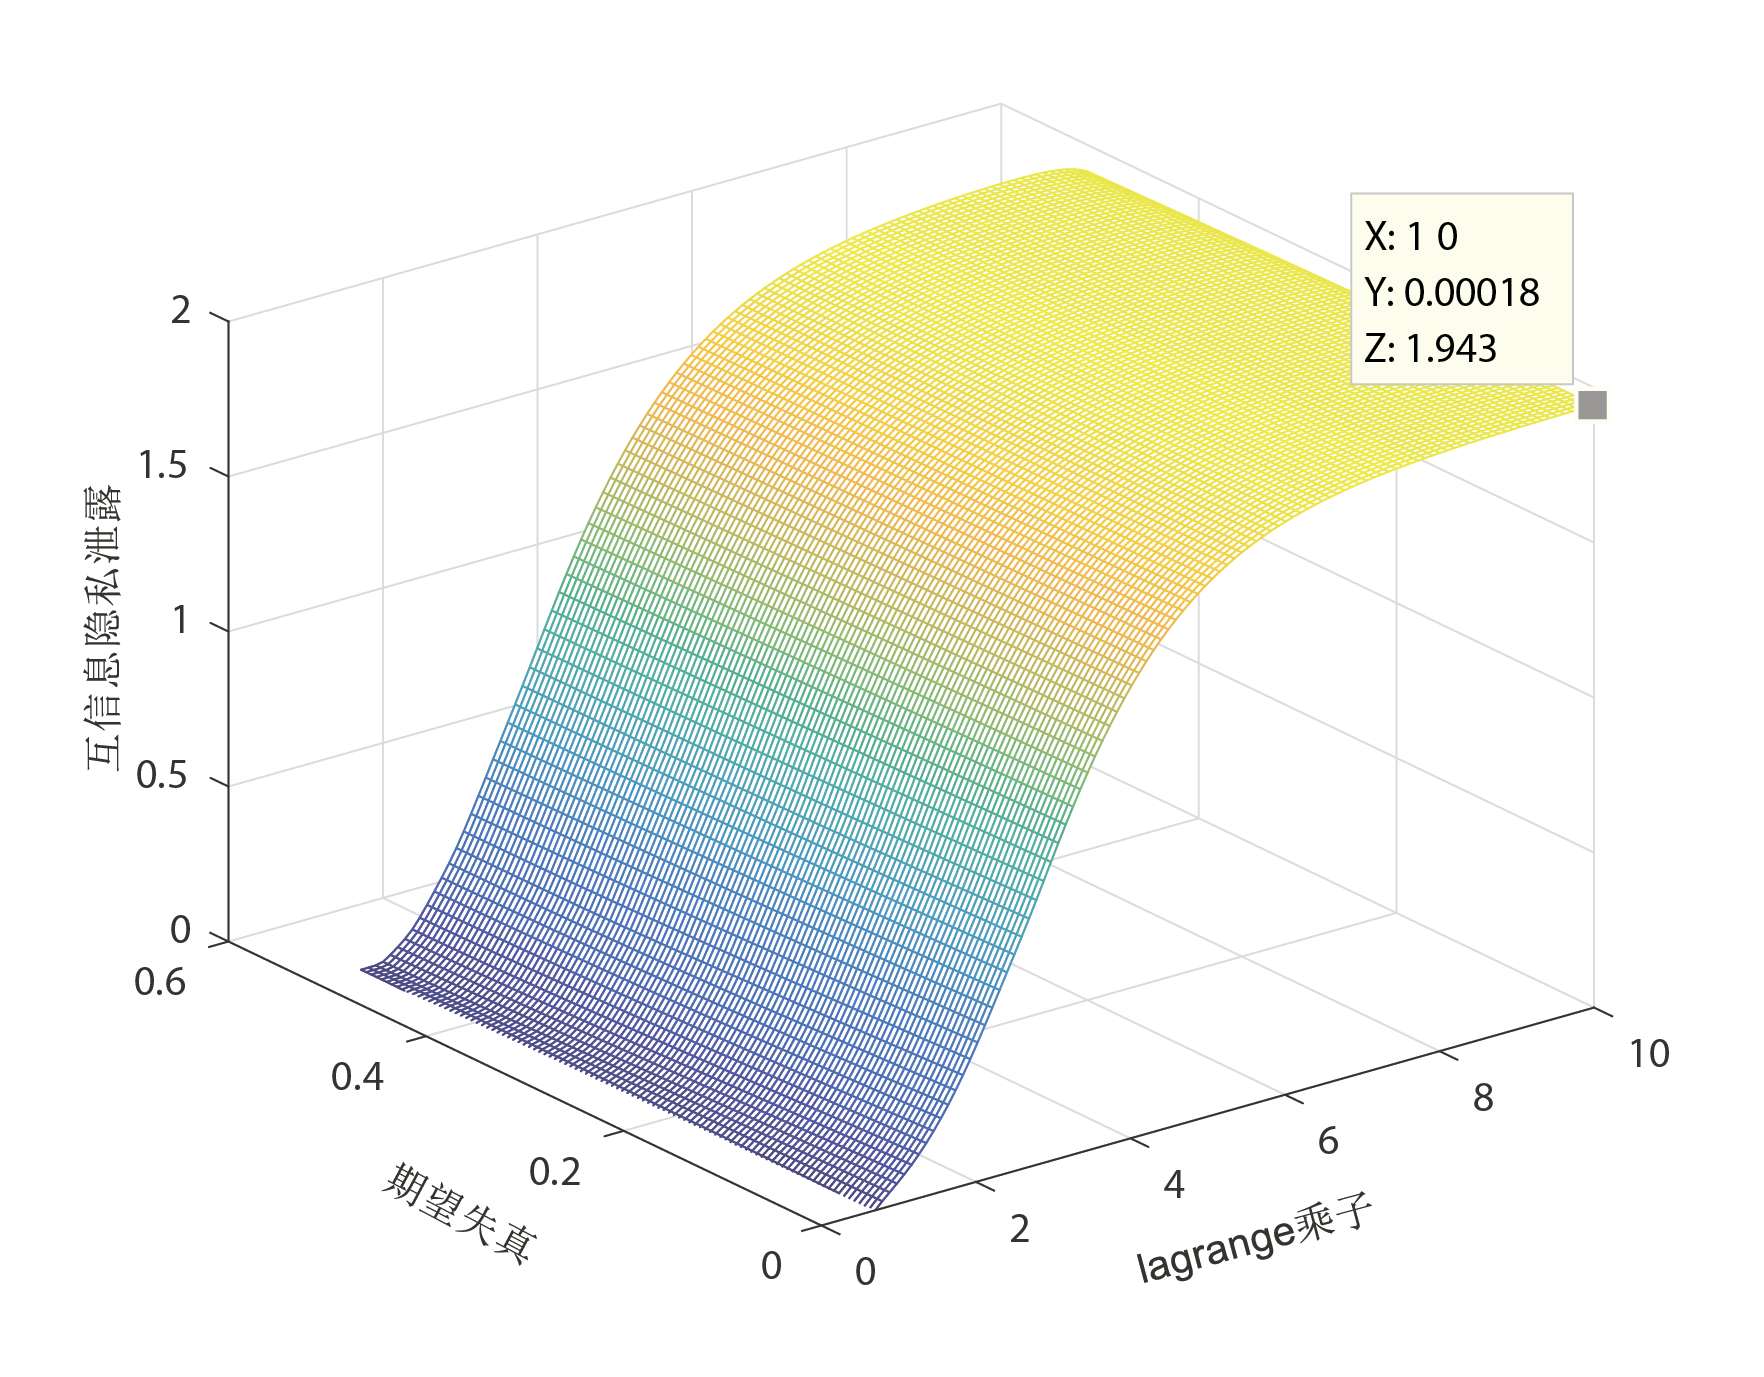
\includegraphics[width=3.5in]{chapter04/Figure4.png}
\caption{ 期望失真、互信息隐私和拉格朗日乘子关系}
\label{Fig:chapter05-4}
\end{figure}
\begin{figure}[htbp]
\centering
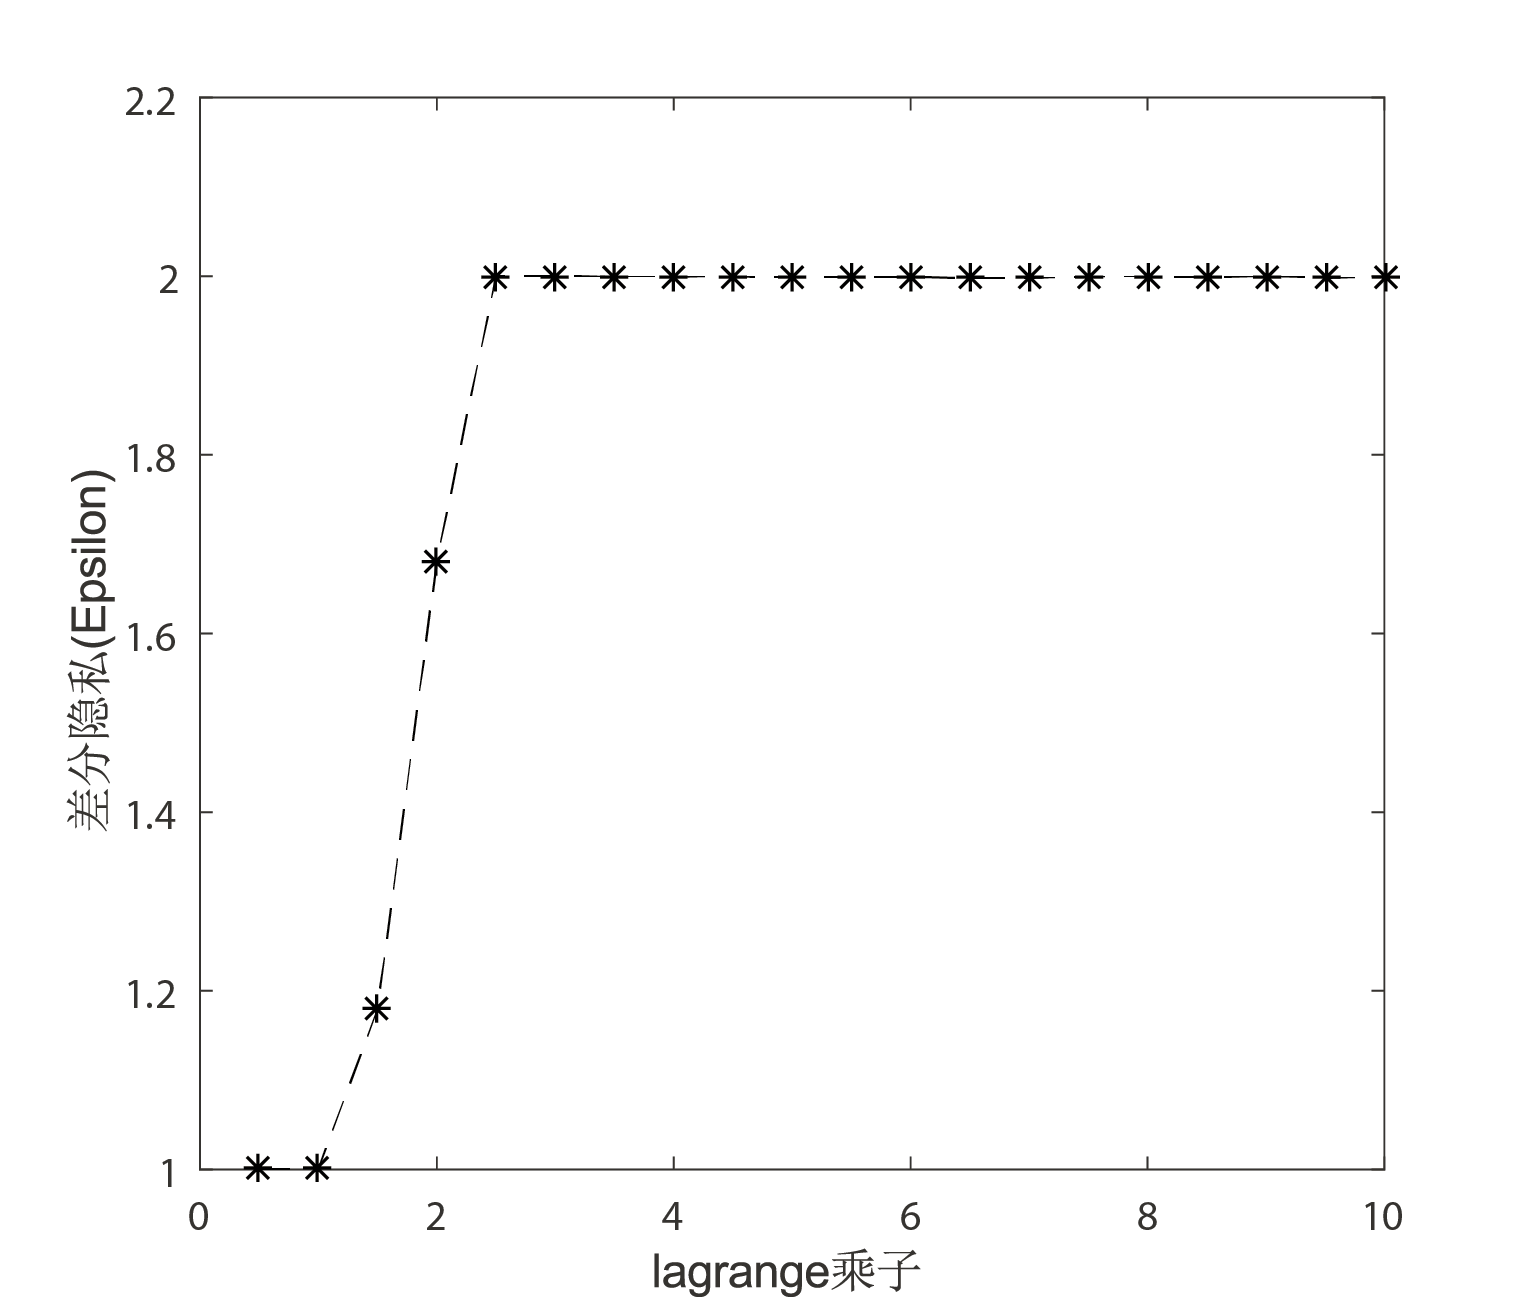
\includegraphics[width=3.5in]{chapter04/Figure5.png}
\caption{拉格朗日乘子与差分隐私参数关系}
\label{Fig:chapter05-5}
\end{figure}

除此之外,实验分析了Lagrange乘子$\lambda$变化对所计算的隐私机制在期望失真和互信息隐私方面的影响。当$T=10^{-8}$时,$\lambda$和互信息隐私、期望失真之间的关系表达为三维图\ref{Fig:chapter05-4}。从图中显示的结果分析,在$\lambda=10.0$时,互信息量$1.943$接近于信源熵$1.9464$,对应的期望失真$0.00018$逼近于$0$,这个关系与图\ref{Fig:chapter05-3}中的曲线图显示结果相吻合。

优化模型迭代求解的算法中$\lambda$和$T$通过影响算法输出的信道条件概率分布进而影响差分隐私保护等级,即隐私预算参数。为了量化隐私机制的不可区分度给出了实验分析。图\ref{Fig:chapter05-5}中展示了信道条件概率满足差分隐私预算参数的曲线(以$\ln$为单位)。从图中所示结果分析,随着$\lambda$变大隐私参数趋近于稳定。结合图\ref{Fig:chapter05-4}和图\ref{Fig:chapter05-5}的结果可知,$\lambda$增加使得互信息隐私量变大,隐私保护的强度变弱,但是,$\lambda$的增加对互信息隐私的影响变弱,使得隐私保护强度无明显变化。


\textbf{(2)} 针对差分隐私数据发布应用中隐私攻击者具有辅助背景知识的优化模型$2$。利用Adult数据集进行实验分析,首先,选择数据集中的Marital-status(婚姻状态)属性,其是类别型属性,域值具有$7$个不同的取值,实验中将其作为发布时的原始数据$X$。其次,由于数据集中Occupation(职业)和Marital-status之间的数据关联,实验中选择Occupation属性,属性域具有$14$个不同的取值,将其考虑为辅助的背景知识$Z$。基于上述数据进行模型$2$的分析,首先,原始数据$X$的概率分布$p(x)=\{0.1386,0.0007,0.4668,0.0127,0.322,0.0312,0.0273\}$,信息熵$H(X)=1.82$。随后,对于类别型属性假设原始与混淆扰动数据域相同,建立汉明失真矩阵。进一步,选择$\lambda \in [0.5,1.0]$,$T=10^{-8}$利用算法\ref{alg:chapter05-1}进行实验。
\begin{figure}[htbp]
\centering
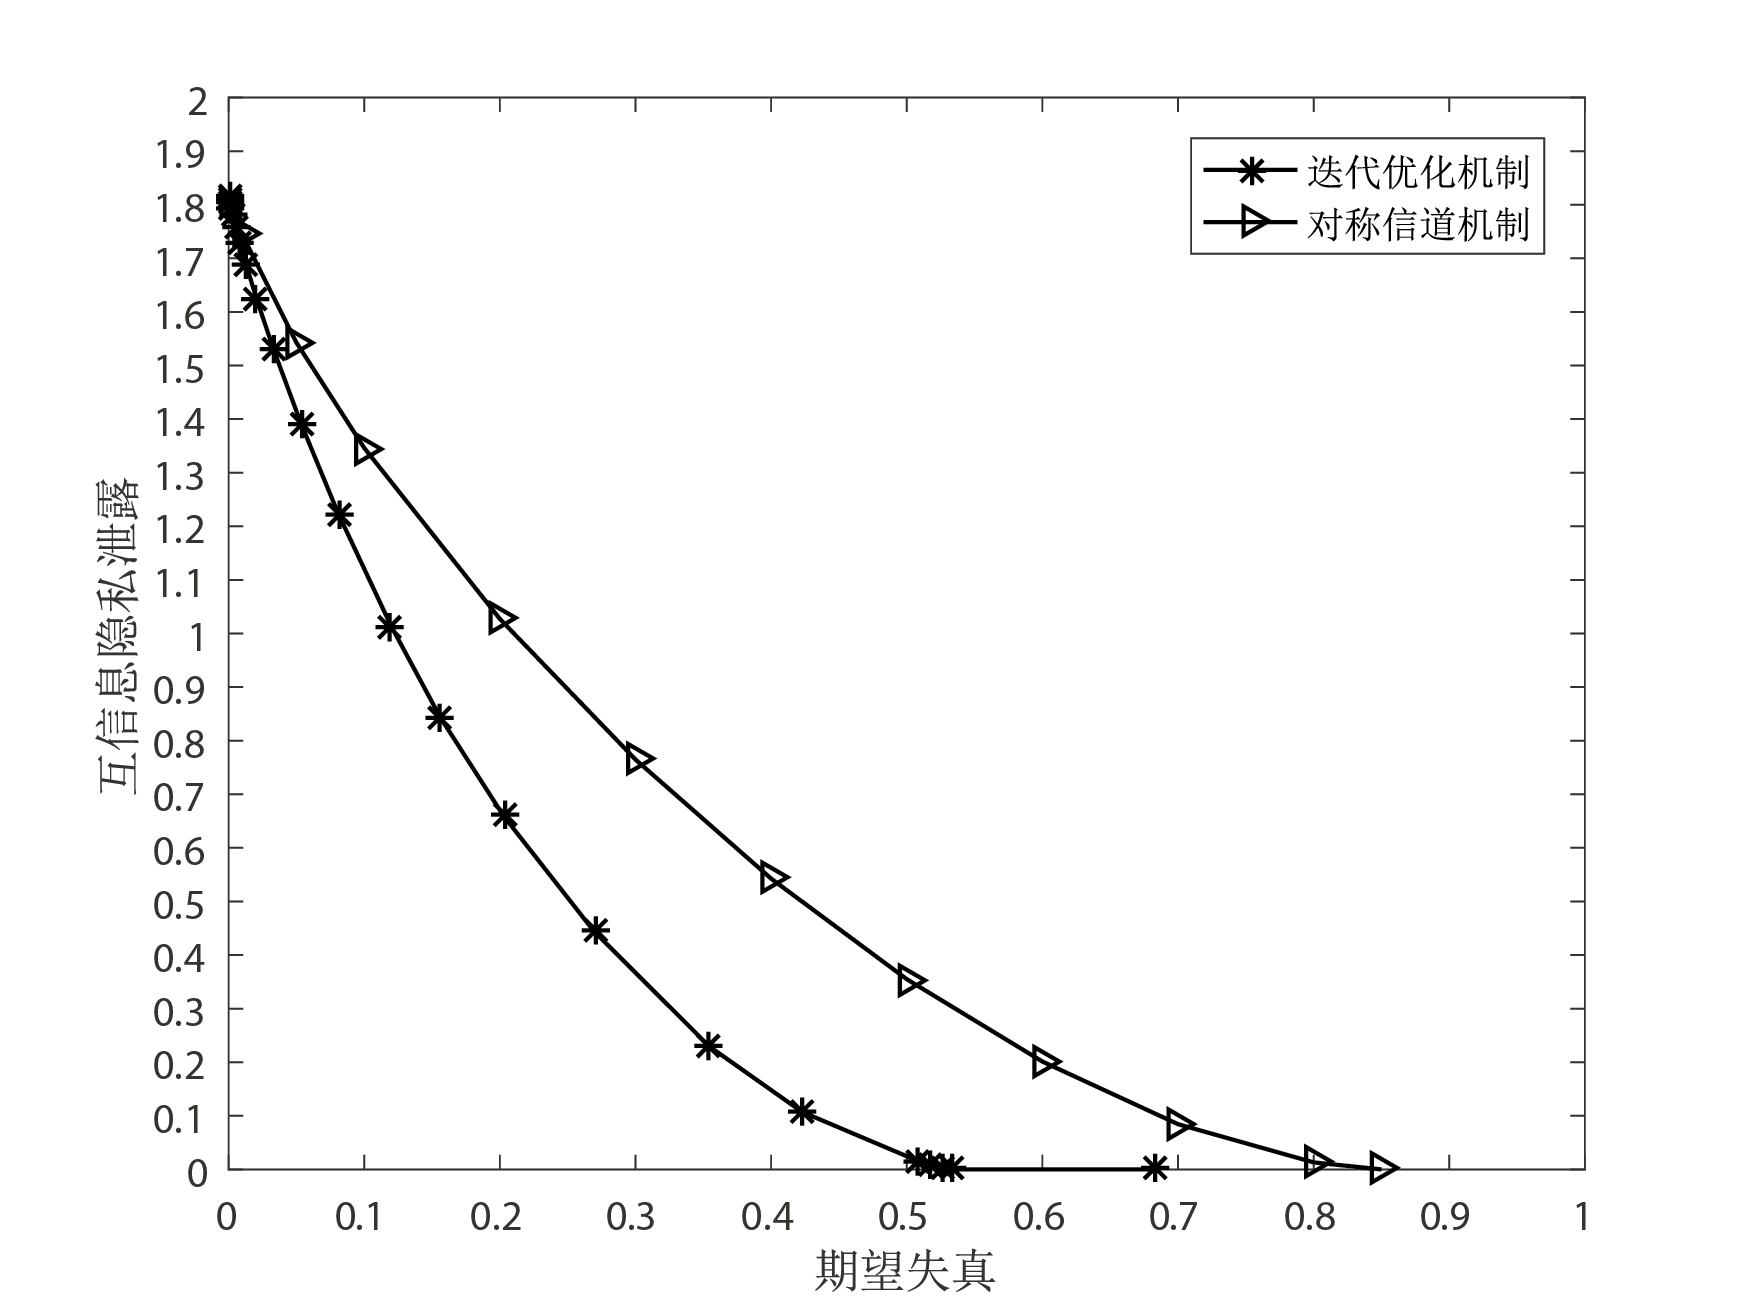
\includegraphics[width=3.5in]{chapter04/Figure6.png}
\caption{两种差分隐私信道机制的对比}
\label{Fig:chapter05-6}
\end{figure}

以下基于本文的隐私与效用度量方法给出实验结果与分析。首先,通过本章中迭代算法求解的隐私信道机制与对称的信道机制在互信息隐私和期望失真度量方面进行对比,比较隐私与数据效用性能。两种不同的信道条件概率分布之间,互信息隐私和期望失真的变化曲线如图\ref{Fig:chapter05-6}所示。图中曲线所示的结果分析,本章中通过优化模型迭代算法求解的隐私机制在同等失真度条件下比对称信道机制表现出更小的互信息隐私泄露。为详细的、定量的表述两种不同隐私机制之间的比较。表\ref{tab:chapter05-1}给出了限失真的互信息隐私泄露量对比数据,表达出同等失真度条件下,迭代优化机制具有相对较小的隐私泄露量。与之对应的,表\ref{tab:chapter05-2}的数据表现出同等隐私泄露容忍度条件下,迭代优化机制拥有相对较小的失真度。结合图\ref{Fig:chapter05-6}及表\ref{tab:chapter05-1}得知,在满足数据质量损失约束前提下,所求解的迭代优化机制比对称信道机制有较好的隐私效果。


\begin{table}
\setstretch{1.1}
\centering
\caption{限失真的互信息隐私泄露量对比}
\label{tab:chapter05-1}
\begin{tabular}{ccc}
  \hline
    机制对比 & 互信息泄露量 & 期望失真\\
  \hline
  对称信道机制 & \tabincell{c}{(0.3397, 0.4963, 0.6379, 0.8387) \\ (1.0185, 1.1587, 1.2761, 1.4166)\\(1.5428, 1.6205, 1.6813, 1.7261)}
   & \multirow{3}{*}{\tabincell{c}{(0.509, 0.423, 0.355, 0.270)\\(0.203, 0.156, 0.120, 0.081) \\ (0.050, 0.033, 0.021, 0.013)}}  \\ 	\cline{1-2}
    迭代优化机制 &  \tabincell{c}{(0.0154, 0.1073, 0.2293, 0.4437) \\ (0.6593, 0.8440, 1.0143, 1.2242)\\(1.3923, 1.5290, 1.6237, 1.6880)}
  &   \\
  \cline{1-3}
\end{tabular}
\end{table}

% \begin{table}[!h]
\begin{table}
\setstretch{1.1}
\centering
\caption{相同互信息隐私泄露的期望失真度对比}
\label{tab:chapter05-2}
\begin{tabular}{ccc}
  \hline
    机制对比 & 期望失真 & 互信息泄露量\\
  \hline
  对称信道机制 & \tabincell{c}{(0.780, 0.675, 0.580) \\ (0.450, 0.345, 0.270)\\(0.205, 0.050, 0.020)}
   & \multirow{3}{*}{\tabincell{c}{(0.02, 0.11, 0.23) \\ (0.44, 0.66, 0.84) \\ (1.01, 1.54, 1.69)}}  \\ 	\cline{1-2}
    迭代优化机制 &  \tabincell{c}{(0.509, 0.423, 0.355) \\ (0.270, 0.203, 0.156)\\(0.120, 0.033, 0.013)}
  &   \\
  \cline{1-3}
\end{tabular}
\end{table}

\begin{figure}[htbp]
\centering
\begin{minipage}[t]{0.48\textwidth}
\centering
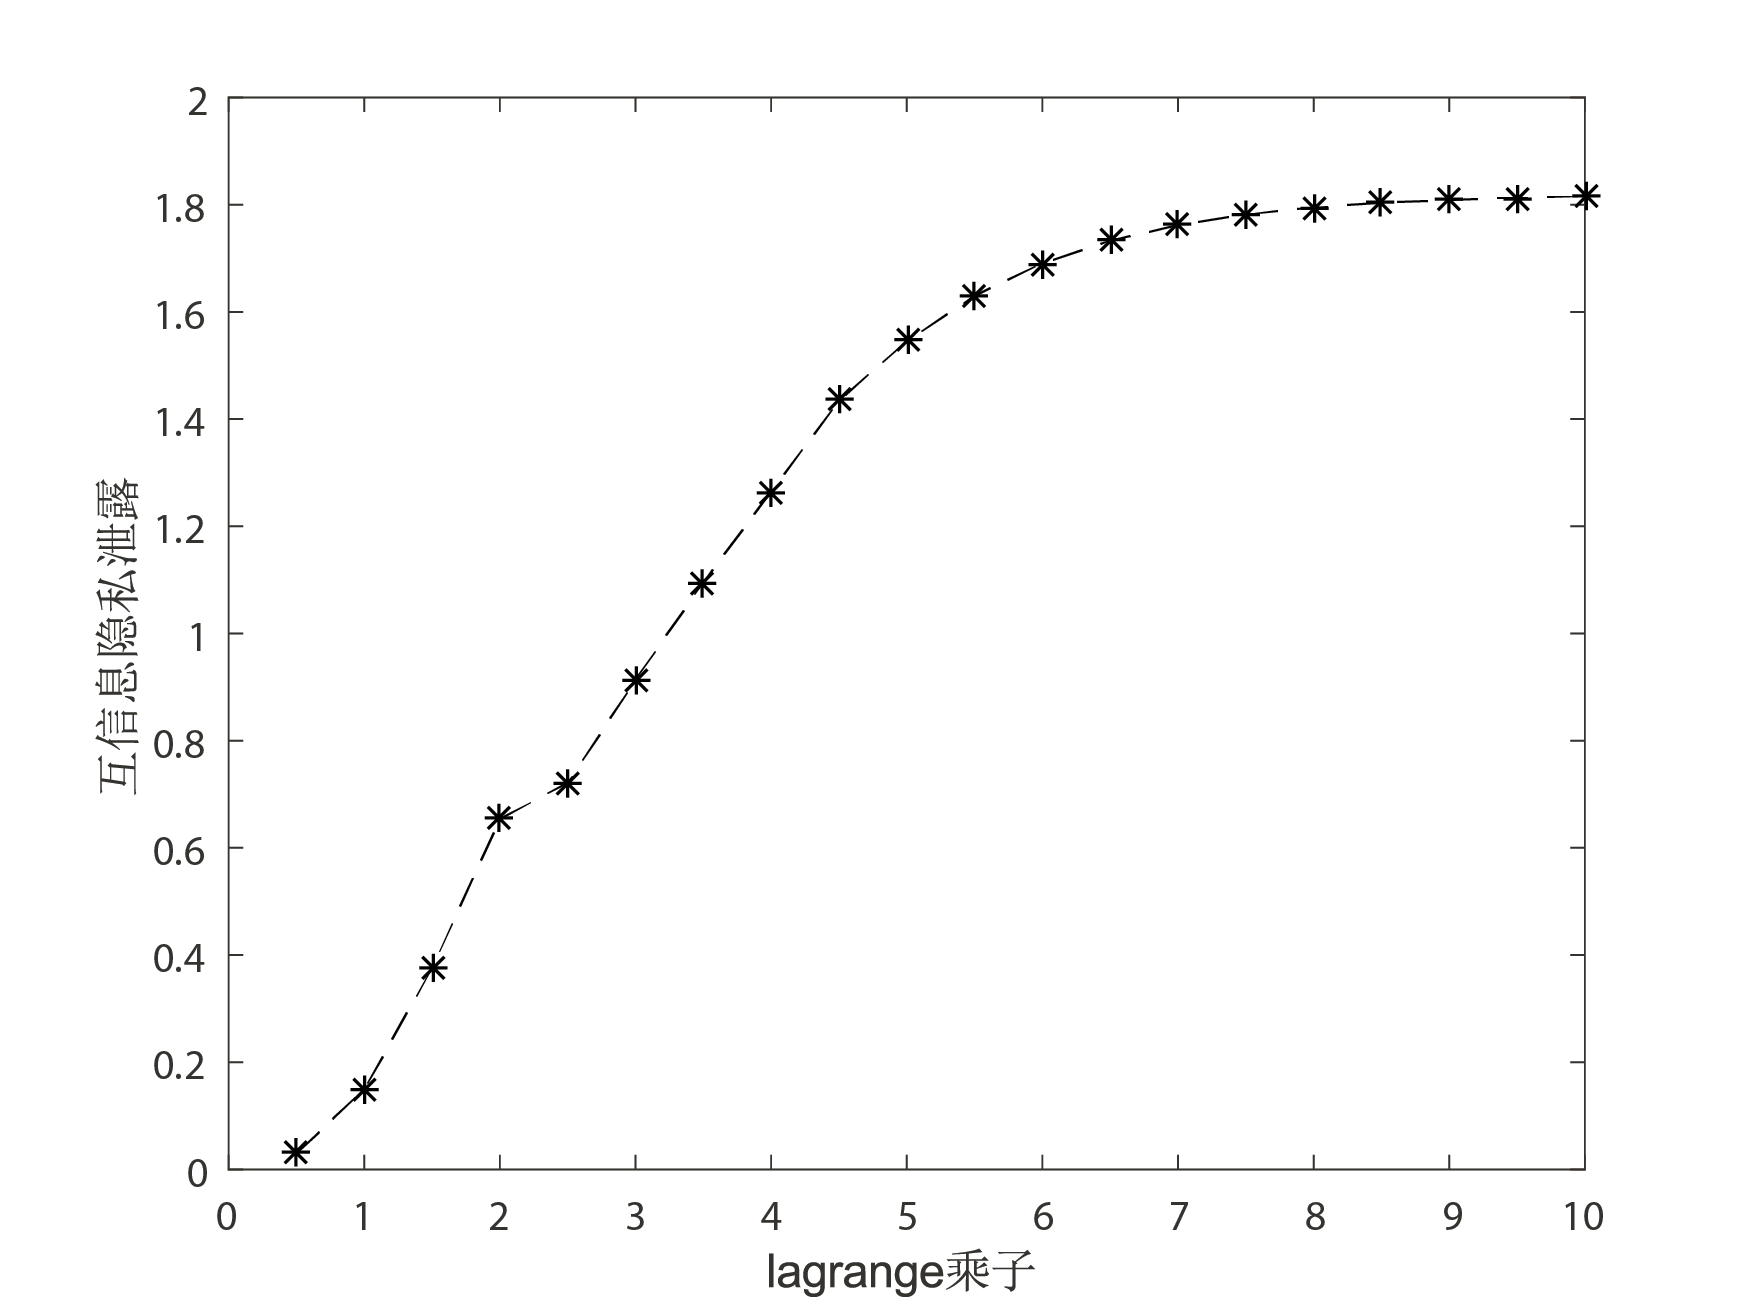
\includegraphics[width=8cm]{chapter04/Figure7.png}
\caption{拉格朗日乘子与互信息隐私泄露}
\label{Fig:chapter05-7}
\end{minipage}
\begin{minipage}[t]{0.48\textwidth}
\centering
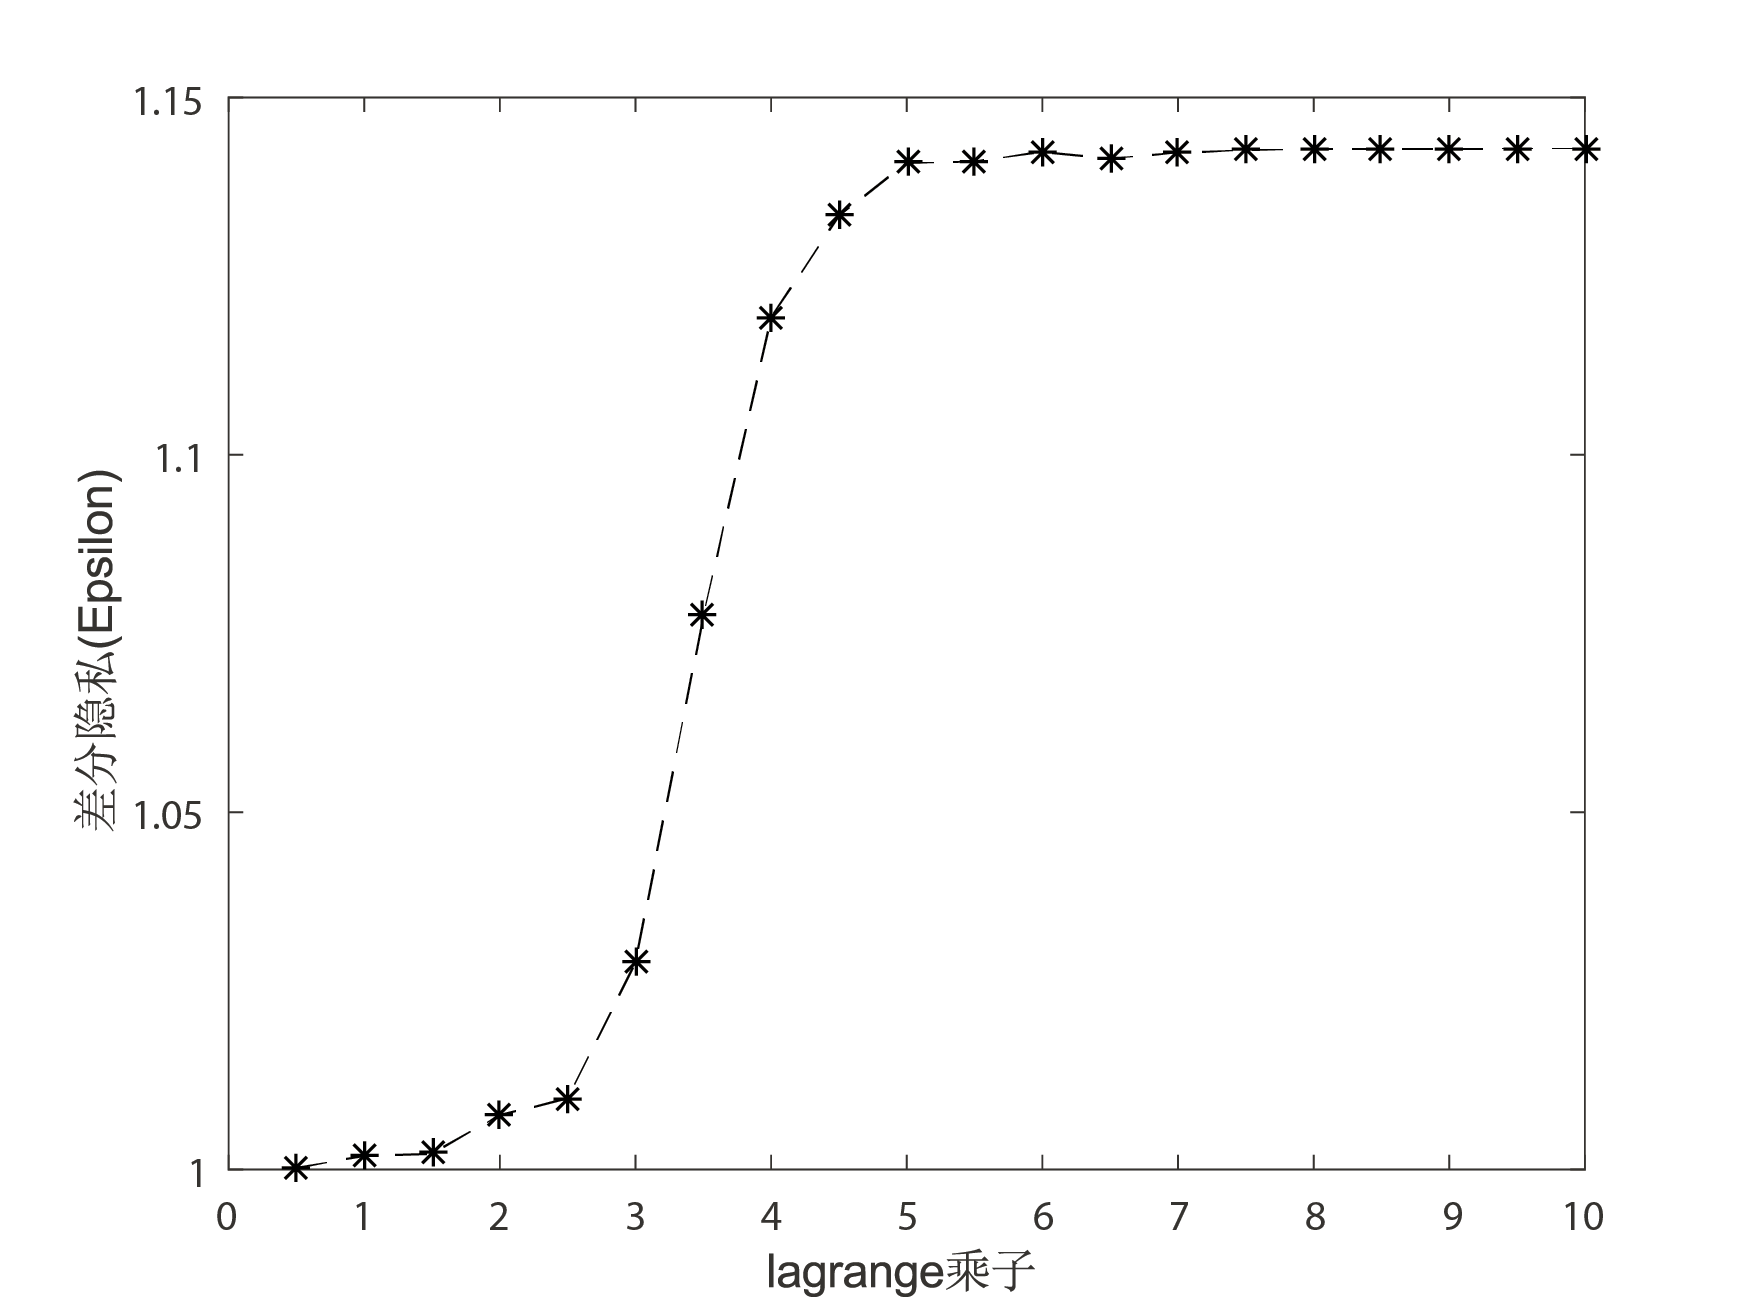
\includegraphics[width=8cm]{chapter04/Figure8.png}
\caption{具有辅助背景知识的$\lambda$与隐私参数}
\label{Fig:chapter05-8}
\end{minipage}
\end{figure}

为研究优化模型$2$的迭代算法中参数对隐私机制条件概率分布的影响,选取$\lambda \in [0.5,10]$,$T=0.01$分析$\lambda$和互信息隐私泄露量、预算参数之间的变化关系。首先,图\ref{Fig:chapter05-7}中展示了$\lambda$和互信息隐私泄露量的变化曲线,结果表明随着$\lambda$的增加,隐私机制的保护强度减弱,互信息隐私泄露量增大。除此之外,曲线的斜率表明了随$\lambda$变大隐私泄露量的增长率下降。当$\lambda \geq 5$时,隐私泄露的变化逐渐呈现平稳的发展趋势。相对应的,隐私预算参数的变化曲线图\ref{Fig:chapter05-8}(图中以$\ln$为单位),结果表明$\lambda$的增加带动了隐私参数的增长,刻画了隐私保护强度的减弱。当$\lambda \geq 5$时,图\ref{Fig:chapter05-8}所表明的结果与图\ref{Fig:chapter05-7}中的结果具有一致性。

更多地,阐述算法中参数$\lambda$,$T$和互信息隐私泄露、期望失真度的关系。实验中设置$\lambda \in \{0.5,1.0,1.5,2.0,2.5\}$、$T\in \{10^{-4},10^{-5},10^{-6},10^{-7},10^{-8}\}$,并组合考虑了不同的$\lambda$和$T$组合。以下给出实验结果的描述。首先,互信息隐私方面,固定$T$ 的取值改变$\lambda$的实验结果如图\ref{Fig:chapter05-9}所示。图中的结果表明,随$\lambda$增加互信息隐私泄露量变大。同时可以看出,选定$\lambda$,$T$的步长以$10$的倍数增长时,互信息隐私泄露量变化较微弱。其次,期望失真的数据质量损失方面,$\lambda$,$T$和期望失真的变化关系如图\ref{Fig:chapter05-10} 所示。图中的结果表明选定$T$时,$\lambda$的变大使得失真损失增加。然而,选定$\lambda$具体取值时,以步长为$10$的数量级增长的$T$并没有引起期望失真的明显变化。基于此说明,在通过算法求解最优信道条件概率分布,设计隐私保护机制阶段,考虑隐私与数据质量需求恰当的选择算法参数$\lambda$和$T$,获得理想的隐私保护效果。
\begin{figure}[htbp]
\centering
\begin{minipage}[t]{0.48\textwidth}
\centering
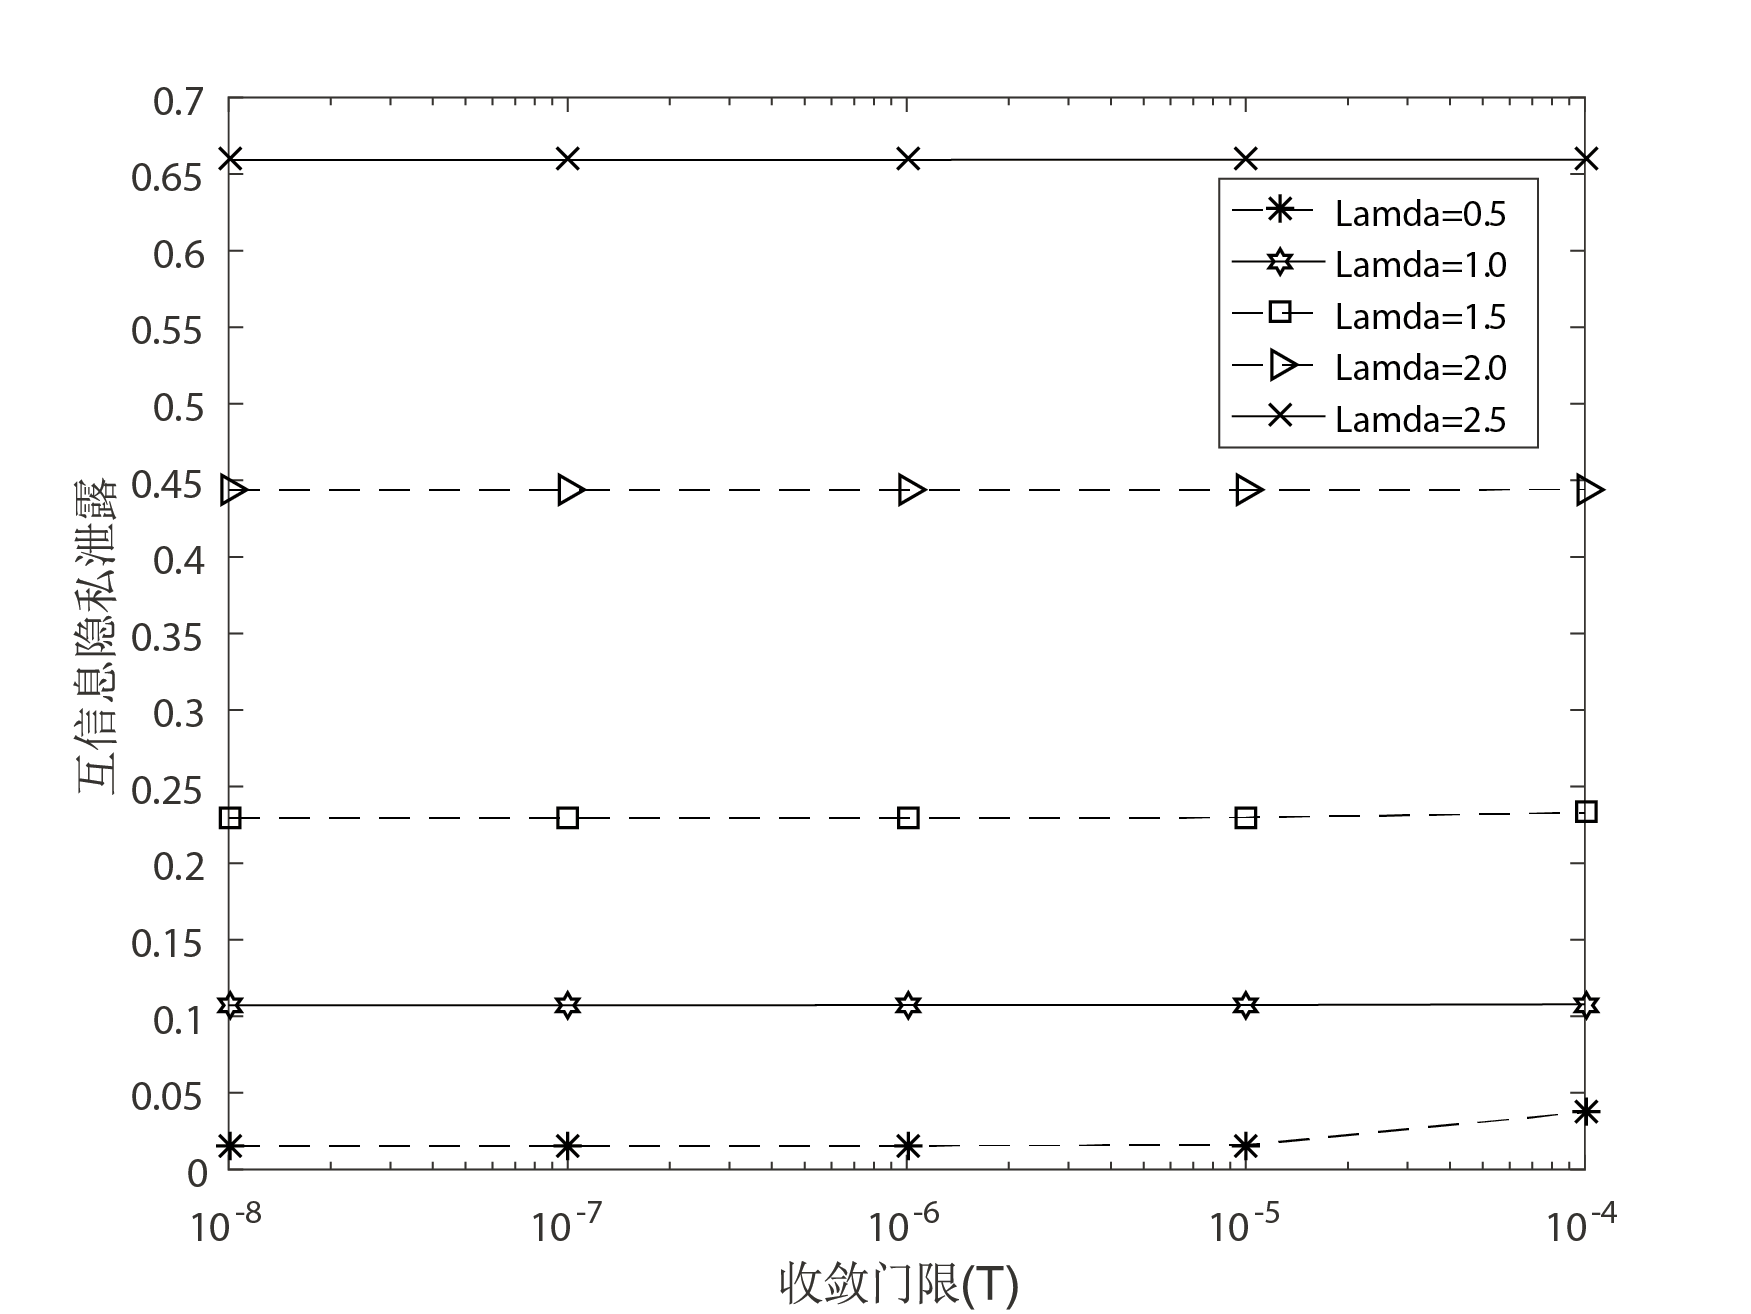
\includegraphics[width=8cm]{chapter04/Figure9.png}
\caption{收敛门限与互信息隐私泄露量}
\label{Fig:chapter05-9}
\end{minipage}
\begin{minipage}[t]{0.48\textwidth}
\centering
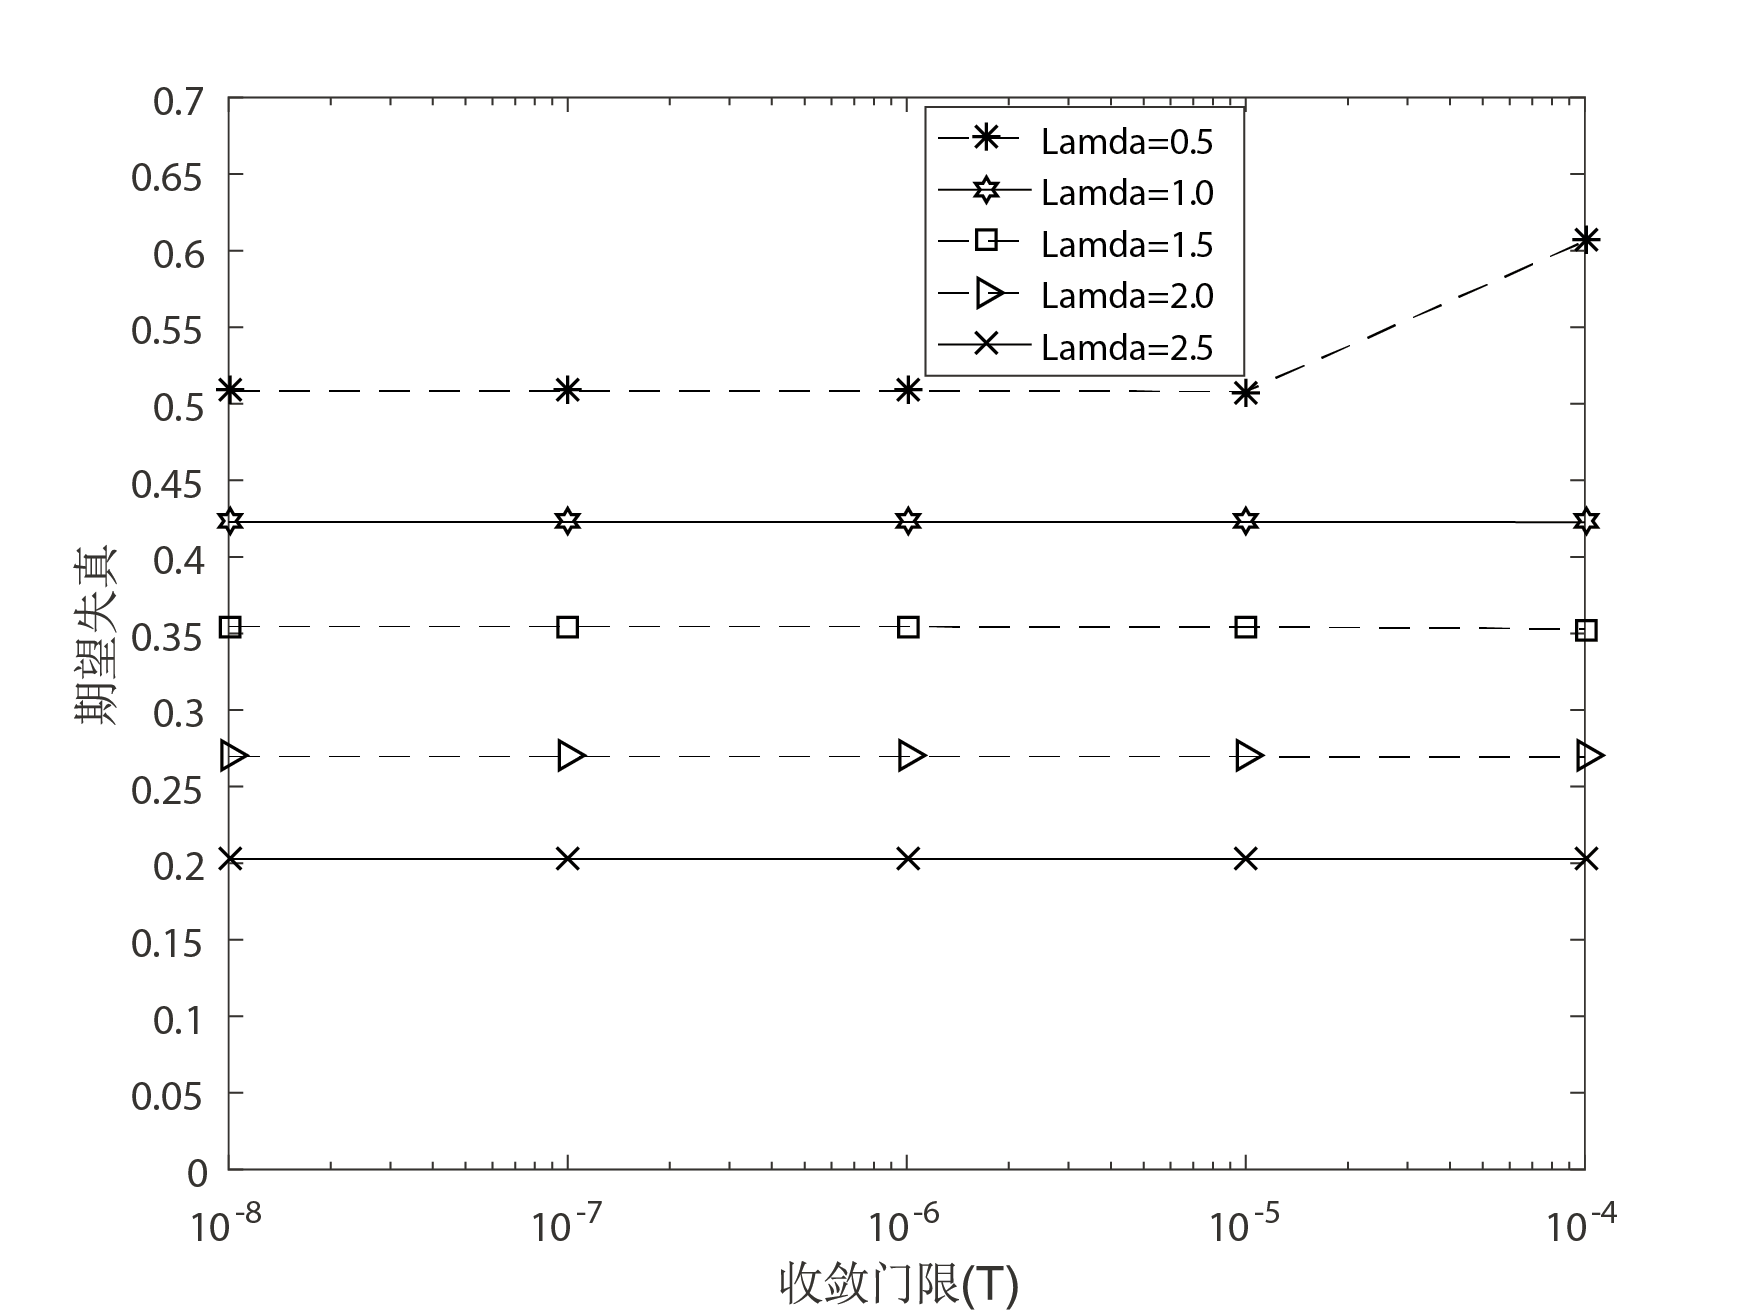
\includegraphics[width=8cm]{chapter04/Figure10.png}
\caption{收敛门限与期望失真度}
\label{Fig:chapter05-10}
\end{minipage}
\end{figure}



本节针对差分隐私数据发布应用中隐私攻击者有或无辅助背景知识的优化模型$1$和$2$,分别采用真实的数据集进行了实验,给出最优化模型迭代计算的差分隐私信道机制在互信息隐私泄露、期望失真方面的分析。在模型$2$求解的隐私机制中,基于隐私与数据可用性的信息论度量对比了对称信道机制。数据结果表明本章中考虑背景知识条件下的迭代优化机制在相同失真下具有比较小的隐私泄露,在相同隐私泄露条件下,所提出的方法具有较高的数据效用。

\section{本章小结}\label{chapter04-conclusion}
本章针对差分隐私数据发布中的隐私保护问题,借鉴Shannon信息论基本通信模型,在隐私与数据效用的度量基础上,利用率失真理论构建了隐私与失真的最优化模型,研究了满足数据质量损失约束条件的互信息隐私最优化机制问题,给出差分隐私数据发布的互信息隐私优化模型。随后,在数据发布的隐私通信模型中,考虑了隐私攻击者可能具有的关联辅助背景知识对互信息隐私泄露的影响,提出了基于联合事件的最小化互信息隐私泄露的优化模型。对于模型求解计算信道条件概率分布的问题,利用拉格朗日乘子法和凸问题的KKT最优性条件,给出解的参量表达式。在迭代算法计算方面,基于率失真函数求解的Blahut-Arimoto算法设计了最优化信道条件概率的迭代求解算法。最后,通过真实数据集上的实验结果,阐述了本章理论部分的研究成果,分析了所提出模型及算法的有效性及优势。

 %基于消解CTL遗忘的计算方法     //  基于消解CTL遗忘的计算方
%\chapter{基于模型的方法计算$\CTL$下的遗忘}\label{chapter05}

{\em
	遗忘理论与均匀插值是一对对偶概念,已有研究表明$\CTL$不具有均匀插值性质~\cite{Maksimova:JANCL:1991},这就表明$\CTL$中的遗忘理论不是封闭的\footnote{对于给定的逻辑语言${\cal L}$和该语言上的操作${\cal O}$,若$\cal O$作用到$\cal L$中的元素后得到的结果仍然在$\cal L$中,则称$\cal O$在$\cal L$下是封闭的。}。
	此时,探索$\CTL$下遗忘理论封闭的情形对深入引用遗忘理论有重要意义。
	为此,本章首先提出有限初始$\MPK$-结构的特征公式;其次,表明$\CTL$公式的遗忘结果在此情形下可以表示成其模型的特征公式的吸取;最后,提出一种基于模型的方法计算遗忘,且探索了如何使用遗忘计算最弱充分条件和知识更新。
}

\section{引言}\label{sec:chapter06_introduction}
%系统模型通常是有限的
%小模型理论,公式的长度有限
%描述数(特征数)来区分同意结构内那些状态在一定程度上是相同的,如果超过这个度,肯定不同。此时,就可以使用CTL公式来描述这些状态及其关系。
%描述forgetting的四个规则。

计算树逻辑是由Clarke和Emerson提出的一种分支时间时序逻辑,它能很好的描述并发系统的一些性质。
Emerson和Halpern证明$\CTL$具有小模型属性:如果一个公式是可满足的,那么它在一个小的有限模型下是可满足的~\cite{DBLP:journals/jcss/EmersonH85}。
具体说来,对于给定的$\CTL$公式$\varphi$,如果公式的长度\footnote{给定公式$\varphi$,出现在该公式里的符号的个数为公式的长度,记为$|\varphi|$。}为$n$(记为:$|\varphi| = n$),则存在一个状态数为$n8^n$的初始$\MPK$-结构$(\Hm,s_0)$使得$(\Hm,s_0)\models \varphi$。

此外,现实情况下能处理的系统都是有限的,且在某一固定环境下所涉及到的原子命题是有限的。因此,在这部分讨论一种约束的$\CTL$,即:(1)出现在$\CTL$公式中的原子命题的个数是有限的(即$\Ha$是有限的);(2)初始结构的状态空间$S$是一个有限的固定状态空间${\cal S}=\{b_1,\ldots,b_m\}$的子集(即$S \subseteq {\cal S}$),且使得对于任意约束长度的$\CTL$公式$\varphi$,若$\varphi$是可满足的,则存在一个初始$\MPK$-结构$(\Hm,s_0)$使得$(\Hm,s_0)\models \varphi$且其状态空间是${\cal S}$的子集。由此可见,在这种情形下只有有限个初始结构应该被考虑。

下文将表明在这一约束条件下$\CTL$中的遗忘是封闭的。

本章其余部分组织如下:首先,第\ref{sec:chapter06_system_model}节介绍本章的基本定义、系统模型,提出研究问题。其次,第\ref{sec:chapter06_our_scheme}节阐述本章中提出的优化模型和ORRP方案。进一步,第\ref{sec:chapter06_privacy_utility_analysis}节给出所提方案在理论上的性能分析。随后,第\ref{sec:chapter05-experiment}节给出真实数据集上的实验结果。最后,在第\ref{sec:chapter05-conclusion}节中进行本章工作总结。

\section{描述初始$\MPK$-结构}\label{sec:chapter06_chaIntC}
本节介绍与一个初始$\MPK$-结构相关的$\CTL$公式——特征公式是如何得到的。
%对于一个给定的有限初始结构(状态个数和$\Ha$都是有限的),其不循环的计算树(状态不重复出现)的深度最多为其状态数的个数。
对于一个给定的初始$\MPK$-结构,其特征公式其计算树的特征公式密切相关。
为此,本节首先介绍计算树之间的$V$-互模拟关系,然后给出计算树的特征公式的定义,最后给出初始$\MPK$-结构的特征公式。

\subsection{计算树的$V$-互模拟}

为此,首先给出能够描述一定深度$n\in \mathbb{N}$的计算树之间的$V$-互模拟关系,记为$\Hb_n^V$。令$V\subseteq \Ha$是原子命题的集合,$i\in \{1,2\}$,$\Hm_i=(S_i,R_i,L_i,s_0^i)$(或$\Hm_i=(S_i,R_i,L_i,[\_]_i,s_0^i)$)是初始结构($\Ind$-Kripke结构),${\cal K}_i=(\Hm_i, s_i)$是$\MPK$-结构(或$\Ind$-结构)。$\Hb_n^V$被递归定义如下:
\begin{itemize}
	\item 若$L_1(s_1)-V=L_2(s_2)$,则$({\cal K}_1,{\cal K}_2) \in \Hb_0^V$;
	\item 对任意$n\ge 0$,若满足下面几个条件,则$({\cal K}_1,{\cal K}_2)\in \Hb_{n+1}^V$成立:
	\begin{itemize}
		\item $({\cal K}_1,{\cal K}_2) \in \Hb_0^V$;
		\item 对任意$(s_1,s_1')\in R_1$,存在$(s_2,s_2')\in R_2$使得$({\cal K}_1',{\cal K}_2') \in \Hb_n^V$;
		\item 对任意$(s_2,s_2')\in R_2$,存在$(s_1,s_1')\in R_1$使得$({\cal K}_1',{\cal K}_2') \in \Hb_n^V$。
	\end{itemize}
\end{itemize}
其中${\cal K}_i'=(\Hm_i,s_i')$。

当所谈及的原子命题的集合$V$很显然的时候,上述$\Hb_n^V$中的$V$可以省略,记为$\Hb_n$。此外,当讨论的$\Hm_i$$(i=1,2)$是显然的时候,可以使用$(s_1,s_2) \in \Hb_n$代替$((\Hm_1,s_1),(\Hm_2,s_2)) \in \Hb_n$。
此时,$V$-互模拟关系就可以定义如下:
\begin{definition}[$V$-互模拟]\label{def:V-bisimulation}
	令$V$是$\Ha$的一个子集,$i\in \{1,2\}$, ${\cal K}_1$和${\cal K}_2$是$\MPK$-结构(或$\Ind$-结构)。
	\begin{itemize}
		\item ${\cal K}_1$和${\cal K}_2$是$V$-互模拟的,当且仅当对所有的$n \ge 0$都有$({\cal K}_1, {\cal K}_2)\in \Hb_n$。若${\cal K}_1$和${\cal K}_2$是$V$-互模拟的,则记为${\cal K}_1 \lrto_V {\cal K}_2$。
		\item 对$\Hm_i$上的路径$\pi_i=(s_{i,1},s_{i,2},\dots)$,若对于任意的$j\in \mathbb{N}_{\ge 1}$\footnote{$\mathbb{N}_{\ge 1}$是大于等于1的整数的集合。}都有${\cal K}_{1,j} \lrto {\cal K}_{2,j}$,则$\pi_1 \lrto_V \pi_2$。其中${\cal K}_{i, j}=(\Hm_i, s_{i,j})$。
	\end{itemize}
\end{definition}

上述$V$-互模拟的定义是现有互模拟定义的一般化,这可以从下面几个方面来体现\footnote{在其他领域也有类似的定义,如:定义在数据库相关文献中的概念$k$-互模拟\cite{kaushik2002updates}。$k$-互模拟概念中涉及与本文$\Hb_n$类似的定义,只是其关系是从相反的方向(即:从孩子到父节点的方向)来说明的。此外,值得一提的是,本文的$V$-互模拟的概念是定义在$\MPK$-结构上的。}。
首先,当给定的$V$为空集且谈论指定的初始状态时,本文的$V$-互模拟与定义在Baier等文章里的互模拟等价(定义7.1\cite{Baier:PMC:2008})的概念一致。
其次,在同一文章里的基于状态的互模拟(定义7.7\cite{Baier:PMC:2008})是定义在给定结构的状态上的,因此与本文的$V$-互模拟(定义在结构的集合上)也不同。
最后,本文的$\Hb_n$的定义与Browne的论文中的状态等价$E_n$类似,只是后者是定义在状态上\cite{browne1988characterizing}而本文的定义在$\MPK$-结构(或$\Ind$-结构)上。


\begin{lemma}
给定原子命题集合$V\subseteq \Ha$和$\MPK$-结构,其中$i=1,2$且$\Hm_i=(S_i, R_i, L_i, s_0^i)$为有限初始结构。$(s_1, s_2)\in \Hb$当且仅当$s_1 \lrto_V s_2$。
\end{lemma}
\begin{proof}
	%由于$\Hb$是${\cal K}_1$和${\cal K}_2$的约束互模拟关系,所以$(s_1, s_2)\in \Hb$。
	值得注意的是对任意的$n\geq 0$,都有$\Hb_{n+1} \subseteq \Hb_n$。又因为$\Hb_0\subseteq S_1 \times S_2$ 是有限的,因而存在一个数$k$使得$\Hb_{k+1}=\Hb_k = \Hb$。
	
	(1)证明若$(s_1, s_2)\in \Hb$则$s_1 \lrto_V s_2$。
	显然,$(s_1, s_2)\in \Hb$。所以,只需要证明$\Hb$是$\Hm_1$和$\Hm_1$之间的一个$V$-互模拟关系。
	下面证明对任意的$r_1\in S_1$和$r_2\in S_2$,$(r_1,r_2) \in \Hb$当且仅当
	\begin{itemize}
		\item[](a) $L_1(r_1)-V = L_2(r_2)-V$;
		\item[](b) $\forall w_1\in S_1$, if $(r_1, w_1)\in R_1$, then $\exists w_2 \in S_2$ s.t. $(r_2,w_2) \in R_2$ and $(w_1, w_2) \in \Hb$; and 
		\item[](c) $\forall w_2\in S_2$, if $(r_2, w_2)\in R_2$, then $\exists w_1 \in S_1$ s.t. $(r_1,w_1) \in R_1$ and $(w_1, w_2)\in \Hb $.
	\end{itemize}

	$(\Rto)$ $(r_1,r_2) \in \Hb$\\
	$\Rto$ $\forall n\geq 0$,$(r_1,r_2)\in \Hb_n$\\
	$\Rto$ $(r_1,r_2)\in \Hb_0$且$\forall n > 0$,$(r_1,r_2)\in \Hb_n$\\
	$\Rto$ $L_1(r_1)-V = L_2(r_2)-V$ (因此,(a)成立),
	
	且$\forall n\geq 0$,$(r_1,r_2)\in \Hb_{n+1}$意味着下面几点成立:
	\begin{itemize}
		\item $L_1(r_1)-V = L_2(r_2)-V$;
		\item $\forall w_1 \in S_1$,若$(r_1, w_1)\in R_1$,则$\exists w_2 \in S_2$使得$(r_2,w_2) \in R_2$且$(w_1, w_2) \in \Hb_n$;且
		\item $\forall w_2\in S_2$,若$(r_2, w_2)\in R_2$,则$\exists w_1 \in S_1$使得$(r_1,w_1) \in R_1$且$(w_1, w_2)\in \Hb_n$。
	\end{itemize}
	
	因为存在一个数$k$使得$\Hb_{k+1}=\Hb_k = \Hb$,所以对这样的$k$有$(r_1,r_2)\in \Hb_{k+1}$使得:
	\begin{itemize}
		\item $L_1(r_1)-V = L_2(r_2)-V$;
		\item $\forall w_1 \in S_1$,若$(r_1, w_1)\in R_1$,则$\exists w_2 \in S_2$使得$(r_2,w_2) \in R_2$且$(w_1, w_2) \in \Hb_k$\\
		$\Rto$ $\forall w_1 \in S_1$,若$(r_1, w_1)\in R_1$,则$\exists w_2 \in S_2$使得$(r_2,w_2) \in R_2$且$(w_1, w_2) \in \Hb$ (因此,(b)成立)。
		\item $\forall w_2\in S_2$,若$(r_2, w_2)\in R_2$,则$\exists w_1 \in S_1$使得$(r_1,w_1) \in R_1$且$(w_1, w_2)\in \Hb_k$\\
		$\Rto$ $\forall w_2\in S_2$,若$(r_2, w_2)\in R_2$,则$\exists w_1 \in S_1$使得$(r_1,w_1) \in R_1$且$(w_1, w_2)\in \Hb$ (因此,(c)成立)。
	\end{itemize}
	
因此,$\Hb$是$\Hm_1$和$\Hm_1$之间的一个$V$-互模拟关系。又因为$(s_1, s_2)\in \Hb$,所以$s_1 \lrto_V s_2$。

$(\Lto)$ 假定(a)、(b)和(c)成立,这里证明$(r_1, r_2)\in \Hb$,即:对于任意的$n\geq 0$都有$(r_1, r_2)\in \Hb_n$。

\begin{itemize}
	\item[(1)]  由(a)可知$(r_1, r_2) \in \Hb_0$,即:$L_1(r_1)-V = L_2(r_2)-V$。
	\item[(2)] 由(b)可知:$\forall w_1 \in S_1$,若$(r_1, w_1)\in R_1$,则 $\exists w_2 \in S_2$使得$(r_2,w_2) \in R_2$且$\forall n\geq 0$都有$(w_1, w_2) \in \Hb_n$ \\ 
	$\Rto$ $\forall w_1 \in S_1$,若$(r_1, w_1)\in R_1$,则$\exists w_2 \in S_2$使得$(r_2,w_2) \in R_2$且$\forall n > 0$都有$(w_1, w_2) \in \Hb_{n-1}$\\
	$\Rto$ $\forall n > 0$,$\forall w_1 \in S_1$,若$(r_1, w_1)\in R_1$,则$\exists w_2 \in S_2$使得$(r_2,w_2) \in R_2$且$(w_1, w_2) \in \Hb_{n-1}$。
	\item[(3)] 由(c)可知:$\forall w_2\in S_2$,若$(r_2, w_2)\in R_2$,则 $\exists w_1 \in S_1$使得$(r_1,w_1) \in R_1$且$\forall n\geq 0$都有$(w_1, w_2)\in \Hb_n$\\
	$\Rto$ $\forall w_2\in S_2$,若$(r_2, w_2)\in R_2$,则$\exists w_1 \in S_1$使得$(r_1,w_1) \in R_1$且$\forall n > 0$都有$(w_1, w_2)\in \Hb_{n-1}$\\
	$\Rto$ $\forall n > 0$,$\forall w_2\in S_2$,若$(r_2, w_2)\in R_2$,则$\exists w_1 \in S_1$使得$(r_1,w_1) \in R_1$且$(w_1, w_2)\in \Hb_{n-1}$。
\end{itemize}

因此,$\forall n > 0$有:
\begin{itemize}
	\item $(r_1, r_2) \in \Hb_0$;
	\item $\forall w_1 \in S_1$,若$(r_1, w_1)\in R_1$,则$\exists w_2 \in S_2$使得$(r_2,w_2) \in R_2$且$(w_1, w_2) \in \Hb_{n-1}$;且
	\item $\forall w_2\in S_2$,若$(r_2, w_2)\in R_2$,则$\exists w_1 \in S_1$使得$(r_1,w_1) \in R_1$且$(w_1, w_2)\in \Hb_{n-1}$。
\end{itemize}
	
所以对于任意的$n\geq 0$都有$(r_1, r_2)\in \Hb$,即:$(r_1, r_2)\in \Hb$。

(ii) 由$s_1 \lrto_V s_2$可知存在$\Hm_1$和$\Hm_1$之间的一个$V$-互模拟关系${\cal R}$使得$(s_1, s_2)\in {\cal R}$。令$\Hb={\cal R}$,显然对任意的$n\geq 0$有$(s_1,s_2)\in \Hb_n$。
	
\end{proof}

给定原子命题集合$V\subseteq \Ha$和初始结构$\Hm_i$($i = 1, 2$)。如果下面条件同时被满足,则称$\Hm_1$的计算树$\Tr_n(s_1)$和$\Hm_2$的计算树$\Tr_n(s_2)$是$V$-互模拟的(记为$({\cal M}_1,\Tr_n(s_1))\lrto_V({\cal M}_2,\Tr_n(s_2))$,简写为$\Tr_n(s_1)\lrto_V\Tr_n(s_2)$):
\begin{itemize}
	\item $L_1(s_1)- V=L_2(s_2)- V$,
	%   \item For every subtree $\Tr_{n-1}(s_i')$ of $\Tr_n(s_i)$,
	%   $\Tr_n(s_{(i \mod 2)+1})$ has a subtree $\Tr_{n-1}(s_{(i \mod 2)+1}')$ such that
	%   $\Tr_{n-1}(s_i')\lrto_V\Tr_{n-1}(s_{(i \mod 2)+1}')$.
	\item 对$\Tr_n(s_1)$的任意子树$\Tr_{n-1}(s_1')$,都存在  $\Tr_n(s_2)$的一棵子树$\Tr_{n-1}(s_2')$使得 
	$\Tr_{n-1}(s_1')\lrto_V\Tr_{n-1}(s_2')$,且
	\item 对任意$\Tr_n(s_2)$的子树$\Tr_{n-1}(s_2')$,都存在$\Tr_n(s_1)$的一棵子树$\Tr_{n-1}(s_1')$使得
	$\Tr_{n-1}(s_1')\lrto_V\Tr_{n-1}(s_2')$。
\end{itemize}

在上述定义中,当$n=0$时,只需考虑第一个条件。

\begin{proposition}\label{B_to_T}
	给定原子命题集合$V\subseteq\cal A$和$\MPK$结构$({\cal M}_i,s_i)$($i=1,2$)。
	则:
	\[(s_1,s_2)\in{\cal B}_n\mbox{当且仅当对任意的$0\le j\le n$有}
	\Tr_j(s_1)\lrto_V\Tr_j(s_2)\mbox{。}\]
\end{proposition}
\begin{proof}
	这里从下面两个方面来证明这一结论:
	
	$(\Rto)$ 这里证明“如果$(s_1, s_2) \in \Hb_n$,则对于任意的$0 \leq j \leq n$有$Tr_j(s_1) \lrto_V Tr_j(s_2)$”成立。$(s_1, s_2) \in \Hb_n$意味着$Tr_n(s_1)$和$Tr_n(s_2)$的根有同样的标签(除了$V$里的元素之外)。
	此外,对任意的$(s_1, s_{1,1}) \in R_1$,存在一个$(s_2, s_{2,1})\in R_2$使得$(s_{1,1}, s_{2,1}) \in \Hb_{n-1}$;且对任意的$(s_2, s_{2,1})\in R_2$,存在一个$(s_1, s_{1,1}) \in R_1$使得$(s_{1,1}, s_{2,1}) \in \Hb_{n-1}$。
	因此,由定义可知$Tr_1(s_1) \lrto_V Tr_1(s_2)$。递归地使用上述方法可得对任意的$0 \leq j \leq n$都有$Tr_j(s_1) \lrto_V Tr_j(s_2)$。
	
	$(\Lto)$这里证明“如果对于任意的$0 \leq j \leq n$有$Tr_j(s_1) \lrto_V Tr_j(s_2)$,则$Tr_j(s_1) \lrto_V Tr_j(s_2)$”成立。
	由$Tr_0(s_1) \lrto_V Tr_0(s_2)$可知$L(s_1) - V = L'(s_2) - V$,因而$(s_1, s_2) \in \Hb_0$。
	由$Tr_1(s_1) \lrto_V Tr_1(s_2)$可知$L(s_1) - V = L'(s_2)- V$,且对于一棵树根的任意后继状态$s$,都能找到另一棵树根的一个后继状态$s'$使得$(s, s')\in \Hb_0$。
	因此有$(s_1, s_2) \in \Hb_1$。同理可证$(s_1, s_2) \in \Hb_2$, \dots, $(s_1, s_2) \in \Hb_n$。
\end{proof}

命题~\ref{B_to_T}表明如果任意两个初始结构中的两个状态$s_1$和$s_2$能够在$\Ha-V$上相互模拟对方直到$n$步,当且仅当分别以$s_1$和$s_2$为根的计算树能在$\Ha-V$上相互模拟直到深度为$n$。
由此可知,如果同一初始结构的两个状态$s$和$s'$不是$V$-互模拟的,则存在一个数$k\in \mathbb{N}$使得分别以$s$和$s'$为根的计算树$\Tr_k(s)$和$\Tr_k(s')$不是$V$-互模拟的。
\begin{proposition}\label{pro:k}
	给定原子命题集合$V\subseteq \Ha$、初始结构$\Hm$和两个状态$s,s'\in S$。
	若$s\not\lrto_V s'$,则存在一个最小整数$k$使得$\Tr_k(s)$和$\Tr_k(s')$不是$V$-互模拟的。
\end{proposition}
\begin{proof}
	若$s\not\lrto_V s'$,则存在一个最小的数$c$使得$(s_i, s_j) \notin \Hb_c$。因此,由命题~\ref{B_to_T}可知,存在一个最小整数$m$($m \leq c$)使得$\Tr_m(s_i)$和 $\Tr_m(s_j)$不是$V$-互模拟的。令$k=m$可得上述结论。
\end{proof}

\subsection{计算树的特征公式}
由上面小节的讨论可知,$V$-互模拟可以将计算树分别开来\footnote{Similar approaches has been taken in the literature e.g., in~\cite{DBLP:conf/birthday/1997ehrenfeucht},  a class (namely, $\equiv_{\overline{k}}$-class) of structures of monadic formulas has been characterized by Hintikka formulas~\cite{hintikka1953distributive}. Another example is Yankov-Fine construction in \cite{yankov1968three}.}。本节讨论如何使用$\CTL$公式描述一棵计算树,且表明具有(或没有)$V$-互模拟关系之间的计算树的特征公式又有怎么样的关系。为此,首先给出计算树的特征公式的定义。
\begin{definition}\label{def:V:char:formula}
	给定原子命题集合$V\subseteq \Ha$、初始结构$\Hm =(S,R,L,s_0)$和状态$s\in S$。
	定义在$V$上的计算树$\Tr_n(s)$的特征公式(记为${\cal F}_V(\Tr_n(s))$,$n\geq 0$)被递归定义如下:
	\begin{align*}
		{\cal F}_V(\Tr_0(s)) &=  \bigwedge_{p \in V\cap L(s)}p
		\wedge \bigwedge_{q\in V-L(s)} \neg q,\\
		{\cal F}_V(\Tr_{k+1}(s))& = \bigwedge_{(s,s')\in R}
		\EXIST \NEXT {\cal F}_V(\Tr_k(s')) 
		\wedge 
		\ALL \NEXT \bigg( \bigvee_{(s,s')\in R} {\cal F}_V(\Tr_k(s')) \bigg) \wedge {\cal F}_V(\Tr_0(s)) \hbox{ ($k\ge 0$)。}
	\end{align*}
\end{definition}

由定义~\ref{def:V:char:formula}可知,计算树的特征公式从三个方面展示了计算树的信息:(1)只考虑$V$中的原子命题;(2)突出了树节点的内容,即:对于任意原子命题$p\in V$,若$p$在节点的标签中,则其正出现在特征公式中,否则负出现在特征公式中;(3)公式中的时序算子表示了状态之间的转换关系。
通俗地讲,${\cal F}_V(\Tr_0(s))$表明了节点$s$的在$V$上的内容;$\EXIST \NEXT$的合取部分和$\ALL \NEXT$部分保证以$s$的每个直接后继状态$s'$为根深度为$k$的计算树都有一个$\CTL$公式来描述。

下面的结论表明,若两个计算树是$V$-互模拟的,则他们在$V$上的特征公式是逻辑等价的。
\begin{lemma}\label{lem:Vb:TrFormula:Equ}
	给定原子命题集合$V\subseteq \Ha$、初始结构$\Hm=(S,R,L,s_0)$和$\Hm'=(S',R',L',s_0')$、$s\in S$、$s'\in S'$且 $n\ge 0$。若$\Tr_n(s) \lrto_{\overline V} \Tr_n(s')$,则${\cal F}_V(\Tr_n(s)) \equiv {\cal F}_V(\Tr_n(s'))$。
\end{lemma}
\begin{proof}
	通过归纳计算树的深度$n$来证明。
	
	\textbf{基始($n=0$):} 对任意的$s_x\in S$和$s_x' \in S'$,若$\Tr_0(s_x) \lrto_{\overline V} \Tr_0(s_x')$,则由$L(s_x) - \overline V = L'(s_x') - \overline V$可知${\cal F}_V(\Tr_0(s_x)) \equiv {\cal F}_V(\Tr_0(s_x'))$。
	
	\textbf{归纳步($n>0$):} 假设对任意的$0\leq m \leq n$若$\Tr_m(s) \lrto_{\overline V} \Tr_m(s')$,则${\cal F}_V(\Tr_m(s)) \equiv {\cal F}_V(\Tr_m(s'))$。
	这里要证明若$\Tr_{n+1}(s) \lrto_{\overline V} \Tr_{n+1}(s')$,则${\cal F}_V(\Tr_{n+1}(s)) \equiv {\cal F}_V(\Tr_{n+1}(s'))$。
	
	由归纳假设可知,对任意的$k=m$、$s_k\in S$ 和$s_k'\in S'$,若$\Tr_{n-k}(s_k) \lrto_{\overline V} \Tr_{n-k}(s_k')$,则${\cal F}_V(\Tr_{n-k}(s_k)) \equiv {\cal F}_V(\Tr_{n-k}(s_k'))$。
	因此,要证原结论成立,只需要证明若$\Tr_{n-k+1}(s_{k-1}) \lrto_{\overline V} \Tr_{n-k+1}(s_{k-1}')$,则${\cal F}_V(\Tr_{n-k+1}(s_{k-1})) \equiv {\cal F}_V(\Tr_{n-k+1}(s_{k-1}'))$。其中,$(s_{k-1},s_k)\in R$且$(s_{k-1}',s_k')\in R'$。
	显然,由计算树的特征公式可知:
	\begin{align*}
		{\cal F}_V(\Tr_{n-k+1}(s_{k-1})) &  =
		\left(\bigwedge_{(s_{k-1},s_k)\in R}
		\EXIST \NEXT {\cal F}_V(\Tr_{n-k}(s_k))\right)
		\wedge \\
		&\ALL \NEXT\left(\bigvee_{(s_{k-1},s_k)\in R}
		{\cal F}_V(\Tr_{n-k}(s_k) )\right)
		\wedge {\cal F}_V(\Tr_0(s_{k-1}))
	\end{align*}
	and
	\begin{align*}
		{\cal F}_V(\Tr_{n-k+1}(s_{k-1}')) &  =
		\left(\bigwedge_{(s_{k-1}',s_k')\in R}
		\EXIST \NEXT {\cal F}_V(\Tr_{n-k}(s_k'))\right)
		\wedge \\
		&\ALL \NEXT\left(\bigvee_{(s_{k-1}',s_k')\in R}
		{\cal F}_V(\Tr_{n-k}(s_k') )\right)
		\wedge {\cal F}_V(\Tr_0(s_{k-1}')).
	\end{align*} 

	又因为$\Tr_{n-k+1}(s_{k-1})$ $\lrto_{\overline V} \Tr_{n-k+1}(s_{k-1}')$,所以对任意的$(s_{k-1}, s_k) \in R$存在$(s_{k-1}', s_k') \in R'$使得$\Tr_{n-k}(s_k) \lrto_{\overline V} \Tr_{n-k}(s_k')$,且对任意的$(s_{k-1}', s_k') \in R'$存在$(s_{k-1}, s_k) \in R$使得$\Tr_{n-k}(s_k) \lrto_{\overline V} \Tr_{n-k}(s_k')$。
	因此,由归纳假设可知${\cal F}_V(\Tr_{n-k+1}(s_{k-1})) \equiv {\cal F}_V(\Tr_{n-k+1}(s_{k-1}'))$。
\end{proof}

此外,对于初始结构$\Hm$上的状态$s$和$s'$,若$(\Hm,s)$是定义在$V$上的根为$s'$深度为$n$的计算树的特征公式,则$s$和$s'$至少属于$\Hb_n$,即:$s$和$s'$能想互模拟至少到第$n$层深度。

\begin{lemma}\label{Bn:to:Tn}
	令$V\subseteq \Ha$、$\Hm=(S, R, L,s_0)$、$\Hm'=(S', R', L',s_0')$、$s\in S$、$s'\in S'$且$n\ge 0$,则:
	\begin{itemize}
		\item[(i)] $({\cal M},s)\models{\cal F}_V(\Tr_n(s))$;
		\item[(ii)] 若$({\cal M},s)\models{\cal F}_V(\Tr_n(s'))$,则
		$\Tr_n(s) \lrto_{\overline V} \Tr_n(s')$。
	\end{itemize}
\end{lemma}
\begin{proof}
	(i) \textbf{基始($n=0$):}从树的特征公式定义可知${\cal F}_V(\Tr_0(s))$是显然的。

	\textbf{归纳步($n>0$):} 假设对任意的$k\geq 0$,$({\cal M},s)\models{\cal F}_V(\Tr_k(s))$,下面证明$({\cal M},s)\models{\cal F}_V(\Tr_{k+1}(s))$,即:
	\begin{equation*}
		({\cal M},s)\models \left(\bigwedge_{(s,s')\in R}
		\EXIST \NEXT T(s')\right)
		\wedge \ALL \NEXT\left(\bigvee_{(s,s')\in R}
		T(s')\right)
		\wedge {\cal F}_V(\Tr_0(s)).
	\end{equation*}
	其中$T(s') ={\cal F}_V(\Tr_k(s'))$。 
	由基始可知$({\cal M},s)\models {\cal F}_V(\Tr_0(s))$。
	由归纳假设可知,对任意的$(s,s') \in R$有$({\cal M}, s') \models {\cal F}_V(\Tr_k(s'))$。因此有$({\cal M},s)\models \EXIST \NEXT {\cal F}_V(\Tr_k(s')$,从而$({\cal M},s)\models \bigwedge_{(s,s')\in R}
	\EXIST \NEXT {\cal F}_V(\Tr_k(s'))$。
	
	同理,对任意的$(s,s') \in R$都有$({\cal M}, s') \models \bigvee_{(s,s')\in R} {\cal F}_V(\Tr_k(s') )$。因此,
	$$({\cal M},s)\models \ALL \NEXT\left(\bigvee_{(s,s')\in R}
	{\cal F}_V(\Tr_k(s') )\right)$$
	
	从而可知对任意的$n\geq 0$,$({\cal M},s)\models{\cal F}_V(\Tr_n(s))$。
	
	
	
	(ii) \textbf{基始($n=0$):}若$(\Hm, s)  \models {\cal F}_V(\Tr_0(s'))$ ,则$L(s) - \overline V = L'(s') - \overline V$。因此$\Tr_0(s) \lrto_{\overline V} \Tr_0(s')$。
	
	\textbf{归纳步($n>0$):} 假定若$({\cal M},s)\models{\cal F}_V(\Tr_{n-1}(s'))$,则$\Tr_{n-1}(s) \lrto_{\overline V} \Tr_{n-1}(s')$。下面证明若$({\cal M},s)\models{\cal F}_V(\Tr_n(s'))$,则
	$\Tr_n(s) \lrto_{\overline V} \Tr_n(s')$。
	
	\begin{itemize}
		\item[(a)] 由基始知$L(s) - \overline V = L'(s') - \overline V$;
		\item[(b)] 因为$(\Hm, s) \models {\cal F}_V(\Tr_n(s'))$,所以$(\Hm, s) \models \ALL \NEXT\left(\bigvee_{(s',s_1')\in R}{\cal F}_V(\Tr_{n-1}(s_1') )\right)$。由此,对于任意的$(s, s_1) \in R$,存在$(s', s_1') \in R'$使得$(\Hm, s_1) \models {\cal F}_V(\Tr_{n-1}(s_1') )$。由归纳假设可知$\Tr_{n-1}(s_1) \lrto_{\overline V} \Tr_{n-1}(s_1')$。即:$\forall (s, s_1) \in R$,$\exists (s', s_1') \in R'$使得$\Tr_{n-1}(s_1) \lrto_{\overline V} \Tr_{n-1}(s_1')$。
		\item[(c)] 因为$(\Hm, s) \models {\cal F}_V(\Tr_n(s'))$,所以$(\Hm, s) \models  \bigwedge_{(s',s_1')\in R'} \EXIST \NEXT {\cal F}_V(\Tr_{n-1}(s_1'))$。由此,对于任意的$(s',s_1')\in R'$,存在$(s,s_1)\in R$使得$(\Hm, s_1) \models {\cal F}_V(\Tr_{n-1}(s_1')$。由归纳假设可知$\Tr_{n-1}(s_1) \lrto_{\overline V} \Tr_{n-1}(s_1')$。即:$\forall (s',s_1')\in R'$,$\exists (s,s_1)\in R$使得$\Tr_{n-1}(s_1) \lrto_{\overline V} \Tr_{n-1}(s_1')$。
	\end{itemize}
\end{proof}

%在引理~\ref{lem:Vb:TrFormula:Equ}中,若令$s'=s$

\subsection{初始$\MPK$-结构的特征公式}
由$V$-互模拟的定义和命题~\ref{pro:k}可以自然地得到一个$V$-互模拟的补概念——$V$-可区分的。
特别地,在命题~\ref{pro:k}中,若初始结构$\Hm$的两个状态$s$和$s'$不是$\overline{V}$-互模拟的(即:$s\not\lrto_{\overline{V}} s'$),则称$s$和$s'$是\emph{$V$-可区分的}。
且用$\dis_V({\cal M},s,s',k)$表示状态$s$和$s'$在命题~\ref{pro:k}中所说的最小数$k$下是$V$-可区分的。
正如下文所说,$V$-可区分这一概念是定义初始$\MPK$-结构的特征公式重要概念。

此外,对于给定的初始结构$\Hm$和原子命题集合$V$,若在$\Hm$中存在两个状态$s$和$s'$是$V$-可区分的,则称$\Hm$是$V$-可区分的。
而对于一个$V$-可区分的初始结构$\Hm$,存在一个一个最小的数$k$使得对于该结构上的任意两个状态$s$和$s'$,若$s$和$s'$是可区分的,则$(s,s')\not \in \Hb_k$。本文称这样的数为$\Hm$关于$V$的\emph{特征数},记为$ch({\cal M},V)$,其定义如下:
\[ch({\cal M},V)=
\left\{
\begin{array}{ll}
	\max\{k\mid s,s'\in S \text{ 且 }\dis_V({\cal M},s,s',k)\}, \qquad \hbox{${\cal M}$ 是 $V$-可区分的;} \\
	\min\{k\mid {\cal B}_{k}={\cal B}_{k+1}, k\ge 0\}, \ \ \ \quad  \qquad \qquad \qquad \hbox{否则。}
\end{array}
\right.
\]

由$ch({\cal M},V)$定义可知,对于任意的$\Hm$和$V$,$ch({\cal M},V)$总是存在的,这体现在两个方面:(1)若$\Hm$是$V$-可区分的,存在两个状态$s$和$s'$是$V$-可区分的,由命题~\ref{pro:k}可知,存在一个数$k$使得$\dis_V({\cal M},s,s',k)$成立;(2)若对于任意$k\geq 0$和$\Hm$上的两个状态$s$和$s'$都有$(s,s')\in \Hb_k$且$\Hb_k =\Hb_{k+1}$,则$ch({\cal M},V)=0$。

非形式化地说,特征数$c=ch({\cal M},V)$将$\Hm$上的状态分为两大类:第一类中的任意两个状态$s$和$s'$是$V$-可区分的,且$(s,s')\not \in \Hb_c$;第二类中状态都是$V$-不可区分的。这也在计算树的特征公式上:

\begin{lemma}\label{div_s}
	令$V\subseteq \Ha$、$\Hm=(S,R,L,s_0)$、$k={ch({\cal M},V)}$且$s\in S$,则
	%There is a formula $\phi$ such that
	\begin{itemize}
		\item[(i)] $(\Hm, s)\models {\cal F}_V(\Tr_k(s))$;
		\item[(ii)] 对任意的$s'\in S$,$({\cal M},s) \lrto_{\overline V} ({\cal M},s')$
		当且仅当$({\cal M},s')\models{\cal F}_V(\Tr_k(s))$。
	\end{itemize}
\end{lemma}
\begin{proof}
	(i) 这由引理~\ref{Bn:to:Tn}易知。
	
	(ii) 令$\phi = {\cal F}_V(\Tr_k(s))$($k$为$\Hm$关于$V$的特征数)。由(i)知 $(\Hm, s) \models \phi$,从而对任意的$s' \in S$,若$s \lrto_{\overline V} s'$,由定理~\ref{thm:V-bisimulation:EQ}和$\IR(\phi, \Ha - V)$知$(\Hm, s') \models \phi$。
	
	假定$(\Hm, s')\models \phi$。若$s \nleftrightarrow_{\overline V} s'$,则$\Tr_k(s) \not \lrto_{\overline V} \Tr_k(s')$,因而由引理~\ref{Bn:to:Tn}可知$(\Hm, s')\not \models \phi$,这与假定矛盾。
\end{proof}

由此,可定义初始$\MPK$-结构的特征公式如下。

\begin{definition}[特征公式]
	给定原子命题集合$V\subseteq\cal A$he和初始\MPK-结构${\cal K}=({\cal M},s_0)$,其中$c=ch({\cal M},V)$。对任意$\Hm$上得状态$s' \in S$,记$T(s') = {\cal F}_V(\Tr_c(s'))$。
	则$\cal K$关于$V$的{\em 特征公式} ${\cal F}_V({\cal K})$为:
	\[T(s_0) \text{ } \wedge \bigwedge_{s\in S}\ALL \GLOBAL\left(
	T(s) \rto
	\bigwedge_{(s,s')\in R}
	\EXIST \NEXT T(s')
	\wedge
	\ALL \NEXT \bigg(\bigvee_{(s,s')\in R}T(s')\bigg)
	\right)
	\]
	
\end{definition}

有时为了凸显出初始结构及其初始状态,也把特征公式写为${\cal F}_V(\Hm, s_0)$。显然,$\IR({\cal F}_V(\Hm, s_0), \overline V)$。此外,在特征公式的定义中,使用了深度为$c$(即:特征数)的计算树的特征公式意在表明对任意$\Hm$上的两个状态$s$和$s'$,$s$和$s'$是$V$-可区分的当且仅当${\cal F}_V(\Tr_c(s))\not \equiv {\cal F}_V(\Tr_c(s'))$。特别地,$T(s_0)$确保了初始\MPK-结构的初始状态被$\CTL$公式描述;其余部分表明了结构$\Hm$上状态之间的转换关系。
下面的例子给出了计算特征公式的一般步骤:

\begin{example}[Continued from Example~\ref{ex:2}]\label{ex:4}
	考虑图~\ref{fig:K2Tree}中左边的初始$\MPK$-结构${\cal K}_2= (\Hm, s_0)$(其最初出现在图~\ref{v1uv2}中)。左边的为$\Hm$上的四棵计算树:从左到右表示以$s_0$为根、深度分别为0、1、2和3的计算树(为简化图,计算树的标签没有给出,但是每个树节点的标签可从${\cal K}_2$找到。)。令$V=\{d\}$,则 $\overline{V}=\{s, se\}$。
	
	因为$L(s_1) - \overline{V} = L(s_2) - \overline{V}$,所以有$\Tr_0(s_1) \lrto_{\overline{V}} \Tr_0(s_2)$。由于存在$(s_1, s_2)\in R$使得对任意的$(s_2, s') \in R$都有$L(s_2)- \overline V \neq L(s') - \overline V$,所以$\Tr_1(s_1) \not \lrto_{\overline{V}} \Tr_1(s_2)$。
	由此可知$s_1$和$s_2$是$V$-可区分的,且$\dis_{V}(\Hm, s_1, s_2, 1)$。
	
	 同样,我们可得到:$\dis_{ V}(\Hm, s_0, s_1, 0)$、$\dis_{V}(\Hm, s_1, s_3', 1)$、$\dis_{V}(\Hm, s_0, s_2, 0)$和$\dis_{ V}(\Hm,$ $s_0, s_3', 0)$。此外,$s_2 \lrto_{\overline V} s_3'$。因此可以计算$\Hm$关于$V$的特征数为:
	 $$ch(\Hm, V)=\max\{k\mid s,s'\in S \text{ and } \dis_{V}({\cal M},s,s',k)\} = 1.$$
	 
	  
	所以,可以由以下步骤计算${\cal K}_2$关于$V$的特征公式:
	\begin{align*}
		{\cal F}_V(\Tr_0(s_0)) &= d, \qquad \quad {\cal F}_V(\Tr_0(s_1)) = \neg d, \\
		{\cal F}_V(\Tr_0(s_2)) &= \neg d,  \qquad  {\cal F}_V(\Tr_0(s_3')) = \neg d,\\
		{\cal F}_V(\Tr_1(s_0)) &= \EXIST\NEXT \neg d \wedge \ALL\NEXT \neg d \wedge d \equiv \ALL\NEXT \neg d \wedge d, \\
		{\cal F}_V(\Tr_1(s_1)) &= \EXIST\NEXT \neg d \wedge \EXIST\NEXT \neg d  \wedge \ALL\NEXT (\neg d \vee \neg d) \wedge \neg d 
		\equiv \ALL\NEXT \neg d \wedge \neg d, \\
		{\cal F}_V(\Tr_1(s_2)) &= \EXIST\NEXT d  \wedge \ALL\NEXT d \wedge \neg d \equiv \ALL\NEXT d \wedge \neg d,\\
		{\cal F}_V(\Tr_1(s_3')) &\equiv {\cal F}_V(\Tr_1(s_2)),\\
		{\cal F}_V(\Hm, s_0)&\equiv \ALL\NEXT \neg d \wedge d \wedge \\
		& \ALL \GLOBAL(\ALL\NEXT \neg d \wedge d \rto \ALL\NEXT(\ALL\NEXT \neg d \wedge \neg d))\wedge \\
		& \ALL \GLOBAL(\ALL\NEXT \neg d \wedge \neg d \rto \ALL\NEXT(\ALL\NEXT d \wedge \neg d)) \wedge\\
		& \ALL \GLOBAL(\ALL\NEXT d \wedge \neg d \rto \ALL\NEXT(\ALL\NEXT \neg d \wedge d)).
	\end{align*}
	
	
	
	\begin{figure*}
		\centering
		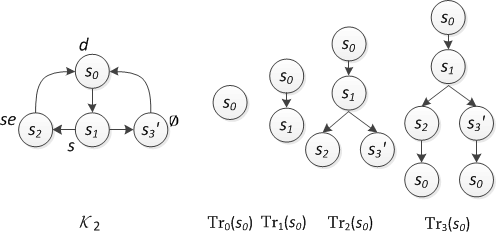
\includegraphics[width=10cm]{chapter05/NK2Tree1.png}
		\caption{左图为初始$\MPK$-结构$\mathcal{K}_2$ (源于图~\ref{v1uv2}); 右图:从左到右表示以$s_0$为根、深度分别为0、1、2和3的计算树(为简化图,计算树的标签没有给出,但是每个树节点的标签可从${\cal K}_2$找到。)}\label{fig:K2Tree}
	\end{figure*}

%\begin{figure*}[!htb]
%	\centering
%	% Requires \usepackage{graphicx}
%	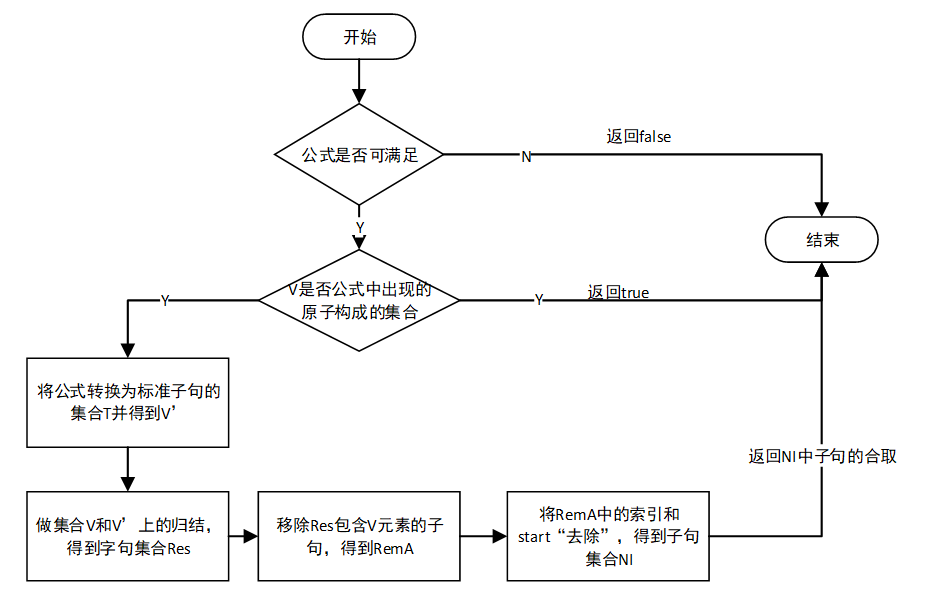
\includegraphics[width=15cm]{chapter04/frame.png}\\
%	\caption{基于归结的遗忘的主要流程图}
%	\label{Fig:chapter05:v1uv2}
%\end{figure*}

\end{example}


下面的定理表示上述定义的特征公式确实描述了一个初始\MPK-结构,此时对系统结构的操作就可转换为对其特征公式的操作,如下文将要讲的给定系统下的最弱充分条件计算。更直观地说,特征公式保持了给定初始$\MPK$-结构在原子命题集合$V$上的所有特性,即:具有$\overline{V}$-互模拟的两个初始$\MPK$-结构关于$V$的特征公式逻辑等价。

\begin{theorem}\label{CF}
	令$V\subseteq \Ha$、$\Hm=(S,R,L,s_0)$且$\Hm'=(S',R', L',s_0')$,则:
	\begin{itemize}
		\item[(i)] $(\Hm',s_0') \models {\cal F}_V({\cal M},s_0)
		\text{ 当且仅当 }
		({\cal M},s_0) \lrto_{\overline V} ({\cal M}',s_0')$;
		
		\item[(ii)] 若$s_0 \lrto_{\overline V} s_0'$则${\cal F}_V(\Hm, s_0) \equiv {\cal F}_V(\Hm', s_0')$。
	\end{itemize}
	
\end{theorem}
\begin{proof}
	(i) 令${\cal F}_V(\Hm, s_0)$为$(\Hm, s_0)$关于$V$的特征公式。显然,$\IR({\cal F}_V(\Hm, s_0), \overline V)$。为了证明上述结论成立,下面证明首先证明$(\Hm, s_0) \models {\cal F}_V(\Hm, s_0)$。
	
	令$c={ch({\cal M},V)}$,由引理~\ref{Bn:to:Tn}可知$(\Hm, s_0) \models {\cal F}_V(\Tr_c(s_0))$。下面证明特征公式里的另一部分,即:$(\Hm, s_0) \models \bigwedge_{s\in S} \ALL\GLOBAL\ G(\Hm, s)$,其中
	\[G(\Hm, s) = {\cal F}_V(\Tr_c(s)) \rto \left(\bigwedge_{(s,s_1) \in R} \EXIST \NEXT {\cal F}_V(\Tr_c(s_1))\right)\wedge \ALL \NEXT \left(\bigvee_{(s,s_1) \in R} {\cal F}_V(\Tr_c(s_1))\right).\]
	
	为此,下面证明$(\Hm, s_0) \models \ALL\GLOBAL\ G(\Hm, s)$。考虑下面两种情况:
	\begin{itemize}
		\item  若$(\Hm, s_0) \not \models {\cal F}_V(\Tr_c(s))$,显然$(\Hm, s_0) \models G(\Hm, s)$;
		\item 若$(\Hm, s_0) \models {\cal F}_V(\Tr_c(s))$:\\
		$(\Hm, s_0) \models {\cal F}_V(\Tr_c(s))$\\
		$\Rto$  $s_0 \lrto_{\overline V} s$ \hfill (引理~\ref{div_s})
		
		$\forall (s, s_1)\in R$:\\
		$(\Hm, s_1) \models {\cal F}_V(\Tr_c(s_1))$  \hfill  ($s_1 \lrto_{\overline V} s_1$)\\
		$\Rto$ $(\Hm, s) \models \bigwedge_{(s,s_1)\in R}\EXIST \NEXT {\cal F}_V(\Tr_c(s_1))$\\
		$\Rto$ $(\Hm, s_0) \models$ $\bigwedge_{(s,s_1)\in R}\EXIST \NEXT {\cal F}_V(\Tr_c(s_1))$    \qquad  ($\IR(\bigwedge_{(s,s_1)\in R}\EXIST \NEXT {\cal F}_V(\Tr_c(s_1)), \overline V)$, $s_0 \lrto_{\overline V} s$)
		
		$\forall (s, s_1) \in R$:\\
		$(\Hm, s_1) \models \bigvee_{(s, s_2)\in R}{\cal F}_V(\Tr_c(s_2))$\\
		$\Rto$ $(\Hm, s) \models \ALL \NEXT \left( \bigvee_{(s, s_2)\in R} {\cal F}_V(\Tr_c(s_2)) \right)$ \\
		$\Rto$ $(\Hm, s_0) \models$  $\ALL \NEXT \left( \bigvee_{(s, s_2)\in R} {\cal F}_V(\Tr_c(s_2)) \right)$   \hfill   ($\IR(\ALL \NEXT \left( \bigvee_{(s, s_2)\in R} {\cal F}_V(\Tr_c(s_2)) \right), \overline V)$, $s_0 \lrto_{\overline V} s$)\\
		$\Rto$ $(\Hm, s_0) \models G(\Hm, s)$。\\
		% where $s_i$ and $s_j$ are the successors of $s$.
	\end{itemize}
	
	对任意其他能从$s_0$可达的状态$s'$,都可以类似地证明$(\Hm,s')\models G(\Hm, s)$。
	因此,对任意的$s\in S$,$(\Hm, s_0) \models \ALL\GLOBAL\ G(\Hm, s)$,从而$(\Hm, s_0) \models {\cal F}_V(\Hm, s_0)$。
	
	下面从两个方面证明(i)成立:
	
	$(\Lto)$ 证明:若$s_0 \lrto_{\overline V} s_0'$,则$(\Hm',s_0') \models {\cal F}_V(M,s_0)$。因为$(\Hm, s_0) \models {\cal F}_V(\Hm, s_0)$且 $\IR({\cal F}_V(\Hm, s_0), \overline V)$,由定理~\ref{thm:V-bisimulation:EQ}可知
	$(\Hm',s_0') \models {\cal F}_V(M,s_0)$。
	
	$(\Rto)$ 证明:若$(\Hm',s_0') \models {\cal F}_V(M,s_0)$,则$s_0 \lrto_{\overline V} s_0'$。为此,下面证明对任意的$n \geq 0$,$Tr_n(s_0) \lrto_{\overline V} Tr_n(s_0')$。
	
	
	\textbf{基始($n=0$):} 由特征公式的定义,显然$Tr_0(s_0) \equiv Tr_0(s_0')$成立。
	
	\textbf{归纳步骤($n>0$):} 假定对任意的$k > 0$都有$\Tr_k(s_0) \lrto_{\overline V} \Tr_k(s_0')$,下面证明$\Tr_{k+1}(s_0) \lrto_{\overline V} \Tr_{k+1}(s_0')$。令$(s_0, s_1), (s_1, s_2)$, $\dots$, $(s_{k-1}, s_k) \in R$且$(s_0', s_1'), (s_1', s_2'), \dots, (s_{k-1}', s_k') \in R'$,即对于任意的$0 \leq i \leq k-1$,$s_{i+1}$($s_{i+1}'$)是$s_i$ ($s_i'$)的直接后继状态。
	由归纳假设可知,只需证明$\Tr_1(s_k) \lrto_{\overline V} \Tr_1(s_k')$。
	
	(a) 由归纳假设可知$L(s_k) - \overline V = L'(s_k') - \overline V$。
	
	在讨论其他点时,首先考虑下面事实(\textbf{fact}):\\
	$(\Hm',s_0') \models {\cal F}_V(\Hm,s_0)$\\
	$\Rto$ $\forall s'\in S'$,$\forall s\in S$,\\ $(\Hm', s')\models {\cal F}_V(\Tr_c(s)) \rto$  $\left(\bigwedge_{(s,s_1)\in R} \EXIST \NEXT {\cal F}_V(\Tr_c(s_1))\right)\wedge \ALL \NEXT \left( \bigvee_{(s,s_1)\in R} {\cal F}_V(\Tr_c(s_1))\right)$  \\
	(I) $(\Hm', s_0') \models {\cal F}_V(\Tr_c(s_0)) \rto \left(\bigwedge_{(s_0, s_1) \in R} \EXIST \NEXT {\cal F}_V(\Tr_c(s_1))\right)$ $\wedge$ $\ALL \NEXT \left(\bigvee_{(s_0, s_1) \in R} {\cal F}_V(\Tr_c(s_1)) \right)$     \\
	(II) $(\Hm', s_0') \models {\cal F}_V(\Tr_c(s_0)))$  \hfill  (已知)\\
	(III) $(\Hm', s_0') \models \left(\bigwedge_{(s_0, s_1) \in R} \EXIST \NEXT {\cal F}_V(\Tr_c(s_1))\right)$ $\wedge$ $\ALL \NEXT \left(\bigvee_{(s_0, s_1) \in R} {\cal F}_V(\Tr_c(s_1)) \right)$  \hfill  ((I),(II))\\
	
	% It is apparent that $L'(s_0') - \overline V = L(s_0) - \overline V$;\\
	(b) 这里证明$\forall (s_k, s_{k+1}) \in R$,存在$(s_k', s_{k+1}') \in R'$使得$L(s_{k+1}) - \overline V = L'(s_{k+1}') - \overline V$。\\
	(1) $(\Hm', s_0') \models \bigwedge_{(s_0, s_1) \in R} \EXIST \NEXT {\cal F}_V(\Tr_c(s_1))$  \hfill  (III)\\
	(2) $\forall (s_0, s_1) \in R$,$\exists (s_0', s_1') \in R'$ 使得 $(\Hm', s_1') \models {\cal F}_V(\Tr_c(s_1))$  \hfill  (1)\\
	(3) $\Tr_c(s_1) \lrto_{\overline V} \Tr_c(s_1')$  \hfill  ((2), 引理~\ref{Bn:to:Tn}) \\
	(4) $L(s_1) - \overline V = L'(s_1') - \overline V$  \hfill   ((3), $c \geq 0)$\\
	(5) $(\Hm', s_1') \models {\cal F}_V(\Tr_c(s_1)) \rto \left(\bigwedge_{(s_1,s_2)\in R} \EXIST \NEXT {\cal F}_V(\Tr_c(s_2))\right) \wedge \ALL \NEXT \left(\bigvee_{(s_1,s_2)\in R} {\cal F}_V(\Tr_c(s_2))\right)$     \hfill  \textbf{(fact)}\\
	(6) $(\Hm', s_1') \models \left(\bigwedge_{(s_1,s_2)\in R} \EXIST \NEXT {\cal F}_V(\Tr_c(s_2))\right) \wedge \ALL \NEXT \left(\bigvee_{(s_1,s_2)\in R} {\cal F}_V(\Tr_c(s_2))\right)$ \hfill ((2), (5))\\
	(7) $\dots \dots$ \\
	(8) $(\Hm', s_k') \models \left(\bigwedge_{(s_k,s_{k+1})\in R} \EXIST \NEXT {\cal F}_V(\Tr_c(s_{k+1}))\right) \wedge \ALL \NEXT \left(\bigvee_{(s_k,s_{k+1})\in R} {\cal F}_V(\Tr_c(s_{k+1}))\right)$       \hfill (与(6)类似)\\
	(9) $\forall (s_k, s_{k+1}) \in R$,$\exists (s_k', s_{k+1}') \in R'$ 使得$(\Hm', s_{k+1}') \models {\cal F}_V(\Tr_c(s_{k+1}))$  \hfill  (8)\\
	(10) $\Tr_c(s_{k+1}) \lrto_{\overline V} \Tr_c(s_{k+1}')$    \hfill ((9), 引理~\ref{Bn:to:Tn}) \\
	(11) $L(s_{k+1}) - \overline V = L'(s_{k+1}') - \overline V$  \hfill   ((10), $c \geq 0)$\\
	
	(c) 这里证明$\forall (s_k', s_{k+1}') \in R'$,存在$(s_k, s_{k+1})\in R$ 使得$L(s_{k+1}) - \overline V = L'(s_{k+1}') - \overline V$。\\
	(1) $(\Hm', s_k') \models \ALL \NEXT \left(\bigvee_{(s_k,s_{k+1})\in R} {\cal F}_V(\Tr_c(s_{k+1}))\right)$  \hfill (上面的(8))\\
	(2) $\forall (s_k', s_{k+1}') \in R'$,$\exists (s_k, s_{k+1}) \in R$ 使得$(\Hm', s_{k+1}') \models {\cal F}_V(\Tr_c(s_{k+1}'))$  \hfill (1) \\
	(3) $\Tr_c(s_{k+1}) \lrto_{\overline V} \Tr_c(s_{k+1}')$    \hfill ((2), 引理~\ref{Bn:to:Tn}) \\
	(4) $L(s_{k+1}) - \overline V = L'(s_{k+1}') - \overline V$  \hfill   ((3), $c \geq 0)$\\
	
	(ii) 由引理~\ref{lem:Vb:TrFormula:Equ}和\ref{div_s}易知。
	
\end{proof}

\section{遗忘理论的封闭性}
当给定的$\CTL$公式的长度(字符的个数)为$n$,由小模型理论可知定义在状态个数为$k=n8^n$的状态空间${\cal S}=\{s_1,s_2,\dots, s_k\}$上的初始结构就能保证公式的可满足性~\cite{DBLP:journals/jcss/EmersonH85}。
对于其他拥有同样大小的状态空间上的任意初始$\MPK$-结构,都能在${\cal S}$状态空间上找到一个初始$\MPK$-结构与之互模拟,且由定理~\ref{CF}可知他们有相同的特征公式。
因此,只有有限个初始$\MPK$-结构作为该公式的候选模型。因此下面结论成立。
%这一事实可以用下面引理表示。

\begin{lemma}\label{lem:models:formula}
	给定$\CTL$公式$\varphi$,下面等式成立:
	\begin{equation*}
		\varphi\equiv \bigvee_{(\Hm, s_0)\in\Mod(\varphi)}{\cal F}_{\cal A}(\Hm, s_0).
	\end{equation*}
\end{lemma}
\begin{proof}
	令$(\Hm', s_0')$为$\varphi$的模型。由定理~\ref{CF}可知$(\Hm', s_0') \models {\cal F}_{\Ha}(\Hm', s_0')$,则:
	$$(\Hm', s_0') \models \bigvee_{(\Hm, s_0)\in \Mod(\varphi)} {\cal F}_{\Ha}(\Hm, s_0).$$
	
	另一方面,假定$(\Hm', s_0')$为$\bigvee_{(\Hm, s_0)\in \Mod(\varphi)} {\cal F}_{\Ha}(\Hm, s_0)$的模型。则存在$(\Hm, s_0)\in \Mod(\varphi)$使得 $(\Hm', s_0') \models {\cal F}_{\Ha}(\Hm,$ $s_0)$。由定理~\ref{CF}可知$(\Hm, s_0) \lrto_{\emptyset} (\Hm', s_0')$,从而由定理~\ref{thm:V-bisimulation:EQ}可知$(\Hm, s_0)$ 是 $\varphi$的一个模型。
\end{proof}

这一结论表明:任意的$\CTL$公式都与其模型的特征公式的吸取逻辑等价。这对遗忘理论的封闭性提供了重要的理论支撑,也即是从公式里遗忘掉原子命题集合$V$中的元素只需找到与给定公式的模型$V$-互模拟的那些模型就能确定遗忘的结果。形式化地,对于给定的公式$\varphi$和原子命题集合$V$,从$\varphi$中遗忘掉$V$中的元素得到的结果为:
\begin{equation*}
	\bigvee_{{\cal K}\in  \{{\cal K}'\mid \exists {\cal K}''\in\Mod(\phi)\ \text{ and }\ {\cal K}''\lrto_V{\cal K}'\}} {\cal F}_{\overline V}({\cal K}).
\end{equation*}


在上述的遗忘理论的定义中说明了如果公式$\psi$的任意一个模型${\cal K}$都能找到$\varphi$的一个模型${\cal K}'$使得${\cal K} \lrto_V {\cal K}'$,则称$\psi$为从$\varphi$中遗忘掉$V$中原子命题后得到的结果。为刻画S5逻辑下该概念的直观含义,Zhang等人提出了如下遗忘理论特性——这些特性被称为\emph{遗忘理论公设}(forgetting postulates)~\cite{Yan:AIJ:2009}。
给定$\CTL$公式$\varphi$、$\varphi'=\CTLforget(\varphi, V)$和原子命题集合$V\subseteq \Ha$和$\varphi'=\CTLforget(\varphi, V)$,遗忘理论公设如下:
\begin{itemize}
	\item[] (\W) 弱(Weakening)属性:$\varphi \models \varphi'$;
	\item[] (\PP) 正支持性(Positive Persistence):对任意与$V$无关的公式$\eta$,若$\varphi \models \eta$则$\varphi' \models \eta$;
	\item[] (\NgP) 负支持性(Negative Persistence):对任意与$V$无关的公式$\eta$,若$\varphi \not \models \eta$则$\varphi' \not \models \eta$;
	\item[] (\textbf{IR}) 无关性(Irrelevance): $\IR(\varphi', V)$
\end{itemize}
直观地说,(\W)和(\textbf{IR})表明“遗忘”削弱了公式$\varphi$且得到的结果与$V$无关,(\PP)和(\NgP)表明对任意与$V$无关的公式$\eta$,$\varphi \models \eta$当且仅当$\varphi' \models \eta$。总而言之,遗忘得到的结果能推出所有与$V$无关且能被$\varphi$推出的结果,且不能推出所有与$V$无关且不能被$\varphi$推出的结果。
从数据库和安全的层面讲,遗忘相当于从已有的关系表中构建出一个视图,达到了隐私保护的作用。
下面的定理表明$\CTL$中的遗忘理论与上述公设也具有当且仅当的关系。

\begin{theorem}[Representation Theorem]\label{thm:close}
	%Let $\varphi$, $\varphi'$ and $\phi$ be \CTL\
	给定$\CTL$公式$\varphi$和$\varphi'$,$V \subseteq \Ha$为原子命题的集合。
	%Then t
	下面的陈述是等价的:
	\begin{itemize}
		\item[(i)] $\varphi' \equiv \CTLforget(\varphi, V)$,
		\item[(ii)] $\varphi'\equiv \{\phi \mid\varphi \models \phi \text{ and } \IR(\phi, V)\}$,
		\item[(iii)] 若$\varphi$、$\varphi'$和$V$为(i)和(ii)中提到的符号,则公设(\W)、(\PP)、(\NgP)和(\textbf{IR})成立. 
	\end{itemize}
\end{theorem}
\begin{proof}
	$(i) \LRto (ii)$. 为了证明这个结论,只需证明如下等式成立:
	\[
	\Mod(\CTLforget(\varphi, V)) = \Mod(\{\phi \mid \varphi \models \phi, \IR(\phi, V)\}).\]
	$(\Rto)$ 对任意$\CTLforget(\varphi, V)$的模型${\cal K}'$ \\
	$\Rto$  $\exists {\cal K}$使得${\cal K} \models \varphi$且${\cal K} \lrto_V {\cal K}'$ \hfill (定义~\ref{def:V:forgetting}) \\
	$\Rto$ $\forall \phi$,若$\varphi \models \phi$且$\IR(\phi, V)$则${\cal K}' \models \phi$  \hfill (定理~\ref{thm:V-bisimulation:EQ})\\
	$\Rto$ ${\cal K}' \models \{\phi \mid \varphi \models \phi, \IR(\phi, V)\}$
	
	$(\Lto)$ 因为$\IR(\CTLforget(\varphi, V),V)$且$\varphi \models \CTLforget(\varphi, V)$,由定义~\ref{def:V:forgetting}可知$\{\phi \mid \varphi \models \phi, \IR(\phi, V)\} \models \CTLforget(\varphi, V)$。
	
	$(ii) \Rto (iii)$.令$A = \{\phi \mid \varphi \models \phi, \IR(\phi, V)\}$。 
	首先,由于对任意的$\phi'\in A$都有$\varphi \models \phi'$,所以$\varphi \models \varphi'$。
	其次,对任意的公式$\phi$,若$\IR(\phi, V)$且$\varphi \models \phi$则$\phi \in A$,因此$\varphi' \models \phi$.
	第三, 对任意的公式$\phi$,若$\IR(\phi, V)$且$\varphi \not \models \phi$则$\phi \not \in A$。因此$\varphi' \not \models \phi$。
	最后,因为对任意的$\phi' \in A$都有$\IR(\varphi',V)$ ,所以$\IR(\phi',V)$。
	
	$(iii) \Rto (ii)$.一方面,由(\PP) 和 (\NgP)可知,对任意的公式$\phi'$且$\IR(\phi',V)$,$\varphi \models \phi'$当且仅当$\varphi' \models \phi'$。所以对任意的$\phi'\in \{\phi \mid \varphi \models \phi, \IR(\phi, V)\}$都有$\varphi' \models \phi'$,因而$\varphi' \models \{\phi \mid \varphi \models \phi, \IR(\phi, V)\}$。 
	另一方面,由 (\W) 和 (\textbf{IR})可知$\{\phi \mid \varphi \models \phi, \IR(\phi, V)\} \models \varphi'$。因此,$\varphi'\equiv \{\phi \mid\varphi \models \phi \text{ and } \IR(\phi, V)\}$。
\end{proof}

\section{基于模型的遗忘理论计算方法}




\section{本章小结}\label{sec:chapter05-conclusion}
本章针对差分隐私数据收集中多维数据处理的隐私脆弱性和有效性问题,为了权衡隐私泄露与数据质量损失,利用信息论的方法提出了有序随机响应扰动(ORRP)方案。首先,对于元组的多维属性使用分治策略思想分解元组属性,构建本地扰动的独立并联信道模型。其次,针对单属性分量的隐私保护问题,基于信息论的度量方法形式化数据质量损失约束前提下最小化隐私信息泄露的最优化模型,用于计算最优概率密度函数(PDF)。然后,以B-A为基本构建模块设计ORRP,利用上述PDF实现有序随机响应,并给出算法描述。最后,给出理论分析和真实数据集上的实验结果。
 %基于模型的CTL遗忘的计算方法  // 差分隐私数据发布的最优化模型
%\chapter{$\mu$-演算中的遗忘理论}
\label{chapter06}

{\em 本章探索$\mu$-演算中的遗忘理论。$\mu$-演算是描述转换系统性质重要逻辑语言,其具有表达能力强的优点:$\mu$-演算是一种表达能力与S2S\footnote{无限完全二叉树下的一元二阶理论(monadic second order theory of the infinite complete binary tree),简称为S2S。}相同的逻辑语言,LTL(线性时序逻辑,linear temporal logic)、CLT和CTL$^*$能表达的属性都能用$\mu$-演算来表示。
	
	已有研究表明$\mu$-演算具有均匀插值性质,这体现了$\mu$-演算下的遗忘理论研究本质上与$\CTL$下的不同。本章首先给出$\mu$-演算下的遗忘理论的定义。其次,表明$\mu$-演算下的遗忘理论是封闭的,这是其与$\CTL$下的遗忘理论的最大的不同。最后,模型检测问题作为形式化验证的重要方法,本章给出$\mu$-演算下遗忘理论的模型检测和推理问题的复杂性结果。
	}

\section{引言}
$\mu$-演算是一种表达能力较强的语言,它能表达$\CTL$不能表示的性质,例如:Kripke结构中有一条路径,在这条路径上的基数状态满足公式$\neg q \wedge \neg p$,但是偶数状态满足$q \wedge p$。这一性质是不能用$\CTL$公式来表示,但是可以用$\mu$-演算公式表示如下:
$$\varphi = \nu X.(p \wedge q) \wedge \EXIST \NEXT(\neg p \wedge \neg q) \wedge \EXIST \NEXT \EXIST \NEXT X.$$

这种情形在日常生活中是很常见的,如:偏序关系$(N, \leq)$(自然数集上的小于等于关系)构成的Kripke结构,其基数节点为基数、偶数节点为偶数。
事实上,$\CTL$不能表达具有有规则的性质~\cite{DBLP:journals/iandc/Wolper83},其主要原因是
\begin{quote}
	\emph{Given a proposition $p$, any proposinal temporal formula (PTL) $f(p)$ containing 
	n ``next" ($\NEXT$) operators has the same truth value on all sequences of the form 
	$p^i(\neg p) p^w$, $i > n$.}
\end{quote}

因而得出如下结论:
\begin{quote}
	\emph{For any given $m\geq 2$, the property ``$p$ is true in every 
	state $s_i$, where $i = km$ (integer $k\geq 0$)" is not expressible in PTL.}
\end{quote}



均匀插值是一个重要的逻辑概念,其有以下含义:给定两个具有$\varphi\models\psi$关系的公式$\varphi$和$\psi$,如果存在公式$\theta$使得$\varphi\models \theta$、$\theta \models \psi$且$\Var(\theta) \subseteq \Var(\varphi) \cap \Var(\psi)$,则称公式$\theta$是$\varphi$和$\psi$的Craig插值。若$\theta$与$\psi$无关,而只与$\Var(\varphi) \cap \Var(\psi)$有关,则称$\theta$为$\varphi$关于$\Var(\varphi) \cap \Var(\psi)$的均匀插值。
均匀插值的定义~\cite{d2006modal}如下(注意:这里的$\Var(\varphi)$表示出现在$\varphi$中的原子命题和变元的集合):                                                                                                                                                                                                                                              
\begin{definition}
	给定一个$\mu$-句子$\varphi$和原子命题的集合$V$,$\varphi$关于$V$的均匀插值是满足下列条件的$\mu$-句子$\theta$:
	\begin{itemize}
		\item $\varphi \models \theta$;
		\item 对任意的公式$\psi$,若$\Var(\varphi) \cap \Var(\psi)\subseteq V$,则$\varphi \models \psi$;
		\item $\Var(\theta) \subseteq V$。 
	\end{itemize}
\end{definition}


从直观上来说,$\varphi$关于$\Var(\varphi) \cap \Var(\psi)$的均匀插值是从$\varphi$中“移除”掉不在$\Var(\varphi) \cap \Var(\psi)$中的原子命题而保留其在$\Var(\varphi) \cap \Var(\psi)$上的结论得到的结果。这与遗忘有着密切的关系。

再者,在背景知识部分已经指出,任意的$\mu$-演算公式都能转换成吸取$\mu$-公式,在这种形式下的公式的均匀插值是容易计算的,即:
\begin{theorem}[定理 3.6~\cite{d2006modal}]
	吸取$\mu$-公式$\varphi$的均匀插值$\exists p \varphi$与$\mu$-公式$\varphi[p/\top, \neg p/ \bot]$等价,其中$\varphi[p/\top, \neg p/ \bot]$是同时将$p$及其否定$\neg p$分别用$\top$和$\bot$替换得到。
\end{theorem}



尽管上面的定义中使用的$\Var(\varphi)$表示出现在$\varphi$中的原子命题和变元的集合,但是均匀插值指的是与原子命题相关的部分,即:对任意的$\mu$-句子$\varphi$和原子命题$p$,存在一个$\mu$-句子$\widetilde{\exists} p. \varphi$使得$\widetilde{\exists} p. \varphi$是$\varphi$关于$\{p\}$的一个均匀插值。这表明在讨论均匀插值时,不考虑变元,即:不是$\varphi$关于某个变元的均匀插值。%实际上,$\mu$-句子里的变元都是受约束的变元。

本章将要说明本文所定义的$\mu$-演算下的遗忘与~\cite{d2006modal}中定义的均匀插值是一对对偶概念,此时本文给出的遗忘的性质无疑也是均匀插值所具有的性质,这为$\mu$-演算的均匀插值的探索提供了另一种思路。此外,借助于均匀插值的计算方法,本文也给出了计算遗忘的方法。这形成了遗忘和均匀插值之间相辅相成的作用。

本章的组织结构如下。首先,给出$\mu$-演算下遗忘的定义;然后,探讨遗忘的一般性质,并给出其与均匀插值的关系;最后给出与遗忘相关的问题的复杂性。

\section{遗忘的定义}\label{sec:chapter06-system-model}
与$\CTL$情形下的遗忘相似,这里先给出$V$互模拟的定义。不失一般性地,令$\Hm_i = (S_i, r_i, R_i, L_i)$,$i$为自然数集$\mathbb{N}$中的元素。
\begin{definition}[$V$-互模拟]\label{def:VB}
	给定原子命题集合$V \subseteq \Ha$和两个Kripke结构$\Hm_1$ 和 $\Hm_2$。若下面几个条件满足,则称$\Hb\subseteq S_1 \times S_2$是$\Hm_1$ 和 $\Hm_2$的$V$-互模拟关系:
	\begin{itemize}
		\item $r_1 \Hb r_2$,
		\item 对任意的$s\in S_1$ 和 $t\in S_2$,若$s \Hb t$ 则对任意的$p \in \Ha- V$有 $p \in L_1(s)$ 当且仅当 $p \in L_2(t)$,
		\item $(s, s')\in R_1$ 和 $s \Hb t$蕴涵存在一个 $t'$ 使得 $s' \Hb t'$ 和 $(t, t')\in R_2$,且
		\item 若 $s \Hb t$ 且 $(t, t')\in R_2$,则存在一个$s'$ 使得 $(s, s')\in R_1$ 和 $t' \Hb s'$。
	\end{itemize}
\end{definition}

与$\CTL$下的$V$-互模拟不同的是,这里要求$r_1 \Hb r_2$(即:$(r_1,r_2)\in \Hb$)。
如果$\Hm_1$ and $\Hm_2$之间存在一个$V$-互模拟关系${\cal B}$则称这两个Kripke结构$\Hm_1$ 和 $\Hm_2$是$V$-互模拟的,记为$\Hm_1 \lrto_V \Hm_2$,
%In this case, $\Hm_1$ and $\Hm_2$ are bisimilar on $V$.
\begin{example}
	如图~\ref{chapter06:fig:bisim}中的两个Kripke结构$\Hm=(S,r,R,L)$ 和 $\Hm'=(S',r',R',L')$,其中:
	\begin{itemize}
		\item $S=\{s_0,s_1,s_2\}$,$S'=\{t_0,t_1\}$,$r=s_0$,$r'=t_0$;
		\item $R=\{(s_0,s_1),(s_1,s_0),(s_0,s_2),(s_2,s_0)\}$,$R'=\{t_0,t_1\}$;
		\item $L(s_0)=\{ch,j\}$,$L(s_1)=L(s_2)=\emptyset$,$L'(t_0)=\{j\}$,$L'(t_1)=\emptyset$。
	\end{itemize}
	由于$\Hm$ 和 $\Hm'$之间存在一个二元$\{ch\}$-互模拟$\Hb=\{(s_0, t_0), (s_1, t_1), (s_2, t_1)\}$ $\Hm \lrto_{\{ch\}} \Hm'$,所以$\Hm\lrto \Hm'$。
	
	
	
	% 	\begin{center}\label{fig:bisim}
	% 		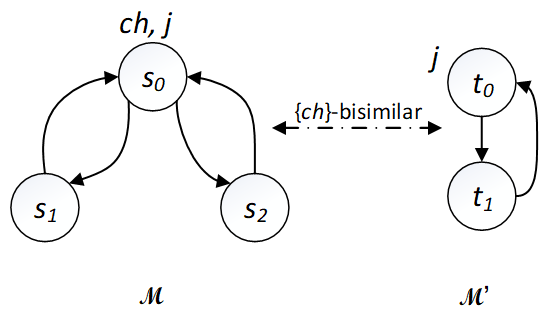
\includegraphics[width=5cm,height=3cm]{chBisimilar.png}\\
	% 		%\vspace{2mm}
	% 		\parbox[c]{7cm}{\textbf{Fig.1~}  Two $\{ch\}$-bisimilar Kripke structures}%\vspace*{.2mm}
	% 	\end{center}
	
	\begin{figure}[h]%
		\centering
		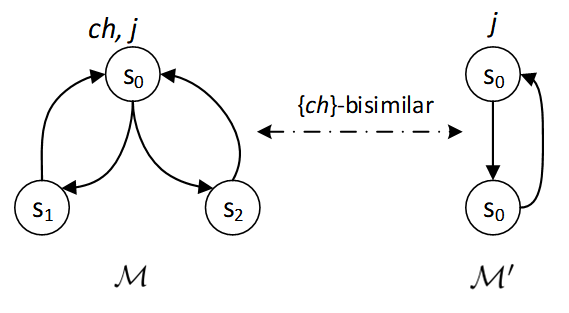
\includegraphics[width=4.5cm,height=2.5cm]{chapter06/chvB.png}
		\caption{两个 $\{ch\}$-互模拟的Kripke结构}\label{chapter06:fig:bisim}
		
		% $s_0$ is labeled by $\{ch, j\}$, $t_0$ is labeled by $\{j\}$, and $s_1$, $s_2$, and $t_1$ are labeled by $\emptyset$.}\label{fig:bisim}
	\end{figure}
	
\end{example}

可以容易证明$\lrto_V$为一个等价关系,此外还有如下性质。

\begin{proposition} \label{pro:EqUnion}
	令$V, V_1 \subseteq \Ha$为原子命题的集合,$\Hm_1$、 $\Hm_2$ 、 $\Hm_3$为Kripke 结构,则:
	\begin{itemize} 
		\item[(i)] $\lrto_V$ 是 Kripke 结构之间的等价关系;
		\item[(ii)] 若 $\Hm_1 \lrto_V \Hm_2$ 且 $\Hm_2 \lrto_{V_1} \Hm_3$,则 $\Hm_1 \lrto_{V \cup V_1} \Hm_3$。
	\end{itemize}
	
\end{proposition}
\begin{proof}
	(i) 这里从自反性、对称性和传递性来证明该关系是一个等价关系。
	
	(1) $\lrto_V$是自反的。容易检查对任意的Kripke结构$\Hm$都有$\Hm\lrto_V \Hm$。
	
	(2) $\lrto_V$ 是对称的。 这里证明对任意的$\Hm_1$ 和 $\Hm_2$,若 $\Hm_1 \lrto_V \Hm_2$ 则 $\Hm_2 \lrto_V \Hm_1$。
	$\Hm_1$和 $\Hm_2$之间存在$V$-互模拟关系$\Hb$,构造如下二元关系$\Hb_1=\{(s,t) \mid (t, s)\in \Hb\}$,现在从下面几点证明$\Hb_1$是$\Hm_2$ 和 $\Hm_1$ 之间的一个$V$-关系:
	\begin{itemize}
		\item 由于$r_1 \Hb r_2$,所以 $r_2 \Hb_1 r_1$,
		\item 对任意的$s\in S_1$ 和 $t\in S_2$,若 $t \Hb_1 s$,则 $s\Hb t$,因此对于任意的$p \in \Ha - V$,$p \in L_1(s)$ 当且仅当 $p \in L_2(t)$,且
		\item 因为$\Hb$是$\Hm_1$和 $\Hm_2$之间存在$V$-互模拟关系,所以$V$-互模拟的第三和第四个点很容易能够证明。
	\end{itemize}
	
	(3) $\lrto_V$是传递的。这里证明对任意的 $\Hm_1$、$\Hm_2$、和 $\Hm_3$,若 $\Hm_1 \lrto_V \Hm_2$ 和 $\Hm_2 \lrto_V \Hm_3$则 $\Hm_1 \lrto_V \Hm_3$。 假定$\Hm_1$和 $\Hm_2$之间存在$V$-互模拟关系为$\Hb_1$,$\Hm_2$和 $\Hm_3$之间存在$V$-互模拟关系$\Hb_2$,构造二元关系: $\Hb=\{(s, z) \mid (s,t) \in \Hb_1,\ (t, z)\in \Hb_2\}$。
	此时,可以像(2)一样证明 $\Hb$ 是$\Hm_1$ 和 $\Hm_3$之间的一个 $V$-互模拟关系。因此,$\Hm_1 \lrto_V \Hm_3$。
	
	(ii) 为了证明$\Hm_1 \lrto_{V\cup V_1} \Hm_3$,只需找到一个  $\Hm_1$ 和 $\Hm_3$之间的二元$(V\cup V_1)$-互模拟关系$\Hb$。
	假定$\Hm_1$和 $\Hm_2$之间存在$V$-互模拟关系为$\Hb_1$,$\Hm_2$和 $\Hm_3$之间存在$V_1$-互模拟关系$\Hb_2$。令$\Hb = \{(s_1, s_3)\mid (s_1, s_2) \in \Hb_1, \ (s_2, s_3) \in \Hb_2\}$,容易证明$\Hb$是$\Hm_1$ 和 $\Hm_3$之间的二元$(V\cup V_1)$-互模拟关系。
\end{proof}

直观地说,(i)表示$\lrto_V$是Kripke结构的集合上的自反、对称和传递关系。
(ii)表示如果一个Kripke结构和其他两个Kripke结构互相$V$和$V_1$互模拟,则这两个Kripke结构$V\cup V_1$-互模拟。这跟$\CTL$情形下的互模拟类似,正如下文将要说到的那样,这一性质有助于证明$\mu$-演算下遗忘的模块属性。

此时,$\mu$-演算下的遗忘如下定义:
\begin{definition}[$\mu$-演算下的遗忘]\label{chapter06:def:V:forgetting}
	令$V\subseteq\cal A$ 和 $\phi$ 为$\mu$-句子。若下面等式成立,则称
	$V$上的 $\mu$-句子 $\psi$是从$\phi$中遗忘掉$V$后得到的结果,记为 $\Muforget(\phi, V)$:
	\begin{equation*}
		\Mod(\psi)=\{\Hm  \mid \exists \Hm' \in\Mod(\phi)\ \&\ \Hm' \lrto_V \Hm\}.
	\end{equation*}
\end{definition}

定义~\ref{chapter06:def:V:forgetting}表明如果 $\psi$ 和 $\psi'$ 都是从$\phi$中遗忘掉 $V$ 中的原子命题得到的结果,则
$\Mod(\psi)=\Mod(\psi')$,也就是说遗忘的结果之间是语义等价的(即有相同的模型)。
%, i.e., $\psi$ and $\psi'$ have the same models. 


D'Agostino 研究了 $\mu$-演算下的均匀插值,并指出 $\mu$-算具有均匀插值性质~\cite{d1996uniform,d2000logical,d2006modal}。换句话说,这意味着对任意的 $\mu$-句子 $\varphi$ 和有限的原子命题的集合$V\subseteq \Var(\varphi)$,都存在一个$V$-无关且与$\varphi$最接近的 $\mu$-句子 $\widetilde{\exists}V \varphi$。
值得注意的是,上述定义的遗忘 $\Muforget(\phi, V)$与 $\widetilde{\exists}V \varphi$~\cite{d2006modal}语义等价.

\section{遗忘的一般属性}
这部分展示$\mu$-演算下遗忘的语义属性。特别地,这里将证明上述$\mu$-演算下的遗忘的定义与遗忘的那几条规则具有“当且仅当的关系”,且从任意$\mu$-句子中遗忘掉任意原子命题的集合的结果总是一个$\mu$-句子。此外,也研究了遗忘算子的代数属性,包括模块性(modularity)、交换性(commutativity)和同质性(homogeneity)。

\begin{theorem} \label{thm:exist}
	给定原子命题 $q \in \cal A$ 和$\mu$-句子 $\phi$,则存在一个$\mu$-句子 $\psi$ 使得 $\IR(\psi, \{q\})$ 且 $\psi \equiv \Muforget(\phi, \{q\})$。
\end{theorem}
\begin{proof}
	已有结果表明,对任意的$\mu$-句子$\phi$和和原子命题$p$,存在一个$\{p\}$-无关的$\mu$-句子$\phi'$(即$\IR(\phi', \{p\})$)使得(定理 3.1 \cite{d1996uniform}):
		\[
	\Hm \models \phi' \mbox{ 当且仅当 } \exists \Hm' \in \phi \mbox{ 使得 } \Hm \lrto_{\{p\}} \Hm'.
	\]
	
	这与本文遗忘的定义一致,因此上述结论成立。
\end{proof}

与模态S5和$\CTL$情形类似,下面给出$\mu$-演算下的遗忘的基本准则:
\begin{itemize}
	\item[(\W)]  削弱(Weakening): $\varphi \models \varphi'$;
	\item[(\PP)]  正支持 (Positive Persistence):
	对任意的$\mu$-句子 $\eta$,若$\IR(\eta, V)$ 和 $\varphi \models \eta$ 则 $\varphi' \models \eta$;
	\item[(\NgP)]  负支持(Negative Persistence):对任意的 $\mu$-句子$\eta$,若$\IR(\eta, V)$ 和 $\varphi \not \models \eta$ 则 $\varphi' \not \models \eta$;
	\item[(\textbf{IR})]  无关性(Irrelevance): $\IR(\varphi', V)$。
\end{itemize}
其中 $V\subseteq\cal A$、
$\varphi$ 为$\mu$-句子 、 $\varphi'$ 是 从$\varphi$中遗忘掉$V$后得到的结果。

\begin{theorem}[表达性定理]\label{chapter06:thm:Rep}
	给定$\mu$-句子 $\varphi$、 $\varphi'$ 和 $\phi$, $V \subseteq \Ha$为原子命题的集合。
	下面的几个陈述是等价的:
	\begin{itemize}
		\item[(i)] $\varphi' \equiv \Muforget(\varphi, V)$,
		\item[(ii)] $\varphi'\equiv \{\phi \mid\varphi \models \phi \text{ 且 } \IR(\phi, V)\}$,
		\item[(iii)] 若$\varphi$、 $\varphi'$ 及 $V$和(i)、(ii)中的符号表示相同公式和原子命题的集合,则 (\W)、 (\PP)、 (\NgP) 和 (\textbf{IR}) 成立。
	\end{itemize}
\end{theorem}
\begin{proof}
	$(i) \LRto (ii)$. 为了证明这一结论成立,只需证明:
	\[
	\Mod(\Muforget(\varphi, V)) = \Mod(\{\phi \mid \varphi \models \phi, \IR(\phi, V)\}).\]
	$(\Rto)$ 对$\Muforget(\varphi, V)$的任意模型 $\Hm'$ \\
	$\Rto$  $\exists\Hm$ 使得 $\Hm \models \varphi$ 和 $\Hm \lrto_V \Hm'$ \hfill (定义~\ref{chapter06:def:V:forgetting}) \\
	$\Rto$ 对于任意与$V$-无关且$\varphi \models \phi$的$\phi$ 都有 $\Hm' \models \phi$ \\
	$\Rto$ $\Hm' \models \{\phi \mid \varphi \models \phi, \IR(\phi, V)\}$
	
	$(\Lto)$ 由于$\IR(\Muforget(\varphi, V),V)$和$\varphi \models \Muforget(\varphi, V)$,由定义~\ref{chapter06:def:V:forgetting}可知 $\{\phi \mid \varphi \models \phi, \IR(\phi, V)\} \models \Muforget(\varphi, V)$。
	
	$(ii) \Rto (iii)$. 为了方便,令$A = \{\phi \mid \varphi \models \phi, \IR(\phi, V)\}$。
	首先,对任意的$A$中的公式$\phi'$都有$\IR(\phi',V)$,所以有$\IR(A,V)$。
	因此,$\IR(\varphi', V)$。 其次,对任意的 $\phi'\in A$,都有$\varphi \models \phi'$,所以$\varphi \models \varphi'$。
	%The (\NgP) and (\PP) are obvious from $A$.
	第三, $\forall \phi$ 且$\IR(\phi, V)$,若$\varphi \models \phi$ 则 $\phi \in A$,因而$\varphi' \models \phi$。
最后, $\forall \phi$ 且 $\IR(\phi, V)$,若 $\varphi \not \models \phi$ 则 $\phi \not \in A$。因此,由定义~\ref{chapter06:def:V:forgetting}和$V$-无关性可知$\varphi' \not \models \phi$。
	
	$(iii) \Rto (ii)$. (1) $\varphi' \models \{\phi \mid \varphi \models \phi, \IR(\phi, V)\}$  \hfill ((\PP))\\
	(2) $\{\phi \mid \varphi \models \phi, \IR(\phi, V)\} \models \varphi'$ \hfill ((\W), (\textbf{IR}))\\
	$\Rto$ $\varphi'\equiv \{\phi \mid\varphi \models \phi, \IR(\phi, V)\}$ \hfill ((1), (2)).
\end{proof}


定理~\ref{chapter06:thm:Rep} 表明$\mu$-演算下的遗忘跟其基本准则形成了一个“当且仅当”的关系:基本准则能描述遗忘的结果,遗忘的结果具有基本准则里的性质。这与S5和$\CTL$下的情形相同。

除了上述的表达性定理,后文将说明准则(\textbf{IR})对计算SNC 和 WSC是重要的。对于$\mu$-句子$\psi = \varphi \wedge (q \lrto \alpha)$,$\varphi \wedge \alpha$ 是 $\{q\}$-无关的,则从$\psi$中遗忘掉 $q$得到的结果是$\varphi$。正如将在第~\ref{chapter07}中展示,这一性质有助于将任意公式的SNC(WSC)转换为命题下的SNC(WSC)。这一性质可形式化如下:

\begin{lemma}
	\label{lem:KF:eq}
	令 $\varphi$ 和 $\alpha$为两个 $\mu$-句子,$q$为原子命题且 $q \not \in  \Var(\varphi) \cup \Var(\alpha)$。则
	$\Muforget(\varphi \wedge (q\lrto\alpha), q)\equiv \varphi$。
\end{lemma}
 \begin{proof}
	令 $\varphi' =\varphi \wedge (q\lrto\alpha)$。对$\Muforget(\varphi', q)$的任意一个模型${\cal M}$,存在一个Kripke结构 ${\cal M}'$使得 ${\cal M}\lrto_{\{q\}}{\cal M}'$ 和 ${\cal M}' \models \varphi'$。显然有 ${\cal M}' \models \varphi$,又因为$\IR(\varphi,\{q\})$ 和 ${\cal M} \lrto_{\{q\}} {\cal M}'$,所以 ${\cal M} \models \varphi$。
	%	by the invariant of $\mu$-sentence for $\overline{V}$-bisimulation~\cite{d1996uniform}.
	
	令 $\Hm \in \Mod(\varphi)$, 其中 ${\cal M}=(S, s, R, L)$。如下构造 $\Hm' = (S, s, R, L')$:
	\begin{align*}
		& L':S \rto 2^{\Ha}\ and\ \forall s^*\in S, L'(s^*) = L(s^*) - \{q\}\ if\ (\Hm, s^*) \not \models \alpha,\\
		& \hbox{否则} L'(s^*) = L(s^*)\cup\{q\}, \\
		& L'(s) = L(s) \cup\{q\}\ if\ (\Hm, s) \models \alpha,\ and\ L'(s) = L(s) \hbox{否则}.
	\end{align*}
	显然 ${\cal M}' \models \varphi$、 ${\cal M}' \models q\lrto \alpha$且
	${\cal M}' \lrto_{\{q\}} {\cal M}$。因此, ${\cal M}' \models \varphi \wedge (q\lrto\alpha)$,又因为${\cal M}' \lrto_{\{q\}} {\cal M}$ 和 $\IR(\Muforget (\varphi \wedge (q\lrto\alpha), q), \{q\})$,所以 ${\cal M} \models \Muforget (\varphi \wedge (q\lrto\alpha), q)$。
\end{proof}


正如在第~\ref{chapter01}中所说的,遗忘在经典命题逻辑中首先被提出,并应用于各种领域。这里给出经典命题逻辑与$\mu$-演算下的遗忘之间的联系。

首先回忆一下从命题公式$\varphi$中遗忘原子命题$p$得到的结果为$\Forget(\varphi, \{p\})\equiv \varphi[p/\bot] \vee \varphi[p/\top]$,且 $\Forget(\varphi, V\cup \{p\})$ 被递归地定义为: $\Forget(\Forget(\varphi, \{p\}),V)$,其中 $\Forget(\varphi, \emptyset) = \varphi$。
此外,对于给定的Kripke结构$\Hm = (S, r, R, L)$和命题公式$\psi$,$\Hm \models  \psi$当且仅当$L(r) \models \psi$。经典命题逻辑与$\mu$-演算下的遗忘之间的联系如下:
\begin{theorem}\label{thm:PL:CTL}
	令$\varphi$为命题公式,$V\subseteq \Ha$为原子命题的集合,则
	\[
	\Muforget(\varphi, V) \equiv \Forget(\varphi, V).
	\]
\end{theorem}
\begin{proof}
	令 $\Hm = (S, r, R, L)$ 和 $\Hm' = (S', r', R', L')$为Kripke结构。
	%容易看出一个 Kripke 结构 $\Hm$$\psi$, i.e., $\Hm \models \psi$, if $L(r)$ satisfies $\psi$.
	
	$(\Rto)$ 对任意的 $\Hm \in \Mod(\Muforget(\varphi, V))$ \\
	$\Rto$ 由定义~\ref{def:V:forgetting}可知$\exists \Hm' \in \Mod(\varphi)$ 使得 $\Hm \lrto_V \Hm'$, %(by a $V$-bisimulation ${\cal B}$) by Def.
	 且$\Hm$和$\Hm'$之间的$V$-互模拟关系为 ${\cal B}$\\
	$\Rto$ $r {\cal B} r'$ \\
	$\Rto$ $\Hm \models \Forget(\varphi, V)$ \hfill ($\IR(\Forget(\varphi, V),V)$, $V$-无关性)
	
	$(\Lto)$ 对任意的 $\Hm \in \Mod(\Forget(\varphi, V))$ \\
	$\Rto$ $\exists \Hm' \in\Mod(\varphi)$ 使得$\forall p \in \Ha-V$, $p \in L(r)$ 当且仅当 $p \in L'(r')$ \hfill ($\Forget$的定义)\\
	%$r {\cal B} r'$\\
	
	如下构造 Kripke 结构 $\Hm_1 = (S_1, r_1, R_1, L_1)$:
	\begin{itemize}
		\item[*] $S_1 = (S - \{r\}) \cup \{r_1\}$,
		\item[*] $R_1$ 与$R$相同,除了$r$被$r_1$替换,且
		\item[*] $L_1$ 与 $L$相同,除了$L_1(r_1) = L'(r')$。
	\end{itemize}
	% $S_1 = (S - \{r\}) \cup \{r_1\}$, $R_1$ is the same as $R$ except that $r$ is replaced by $r_1$, and $L_1$ is the same as $L$ except $L_1(r_1) = L'(r')$. \\
	$\Rto$ $\Hm_1 \models \varphi$ 且 $\Hm_1 \lrto_V \Hm$\\
	$\Rto$ $\Hm \models \Muforget(\varphi, V)$ \hfill ($\IR(\Muforget(\varphi, V), V)$, $V$-无关性)
\end{proof}

定理~\ref{thm:PL:CTL}表明$\mu$-演算下的遗忘是命题逻辑的遗忘的扩展,这提示我们是否命题情形下的遗忘拥有的性质$\mu$-演算下的遗忘也具有。
下面的性质在命题逻辑、S5~\cite{Yan:AIJ:2009} 和$\CTL$中都成立,接下来也证明其在$\mu$-演算中也成立。
\begin{proposition}
	\label{chapter06:pro:ctl:forget:1}
	给定$\mu$-句子$\varphi$、$\varphi_i$和 $\psi_i$ ($i=1,2$),$V\subseteq \Ha$为原子命题的集合。则:
	\begin{itemize}
		\item[(i)] $\Muforget(\varphi, V)$ 是可满足的当且仅当$\varphi$是可满足的;
		\item[(ii)] 若 $\varphi_1 \equiv \varphi_2$,则 $\Muforget(\varphi_1, V) \equiv \Muforget(\varphi_2, V)$;
		\item[(iii)] 若 $\varphi_1 \models \varphi_2$,则 $\Muforget(\varphi_1, V) \models \Muforget(\varphi_2, V)$;
		\item[(iv)] $\Muforget(\psi_1 \vee \psi_2, V) \equiv \Muforget(\psi_1, V) \vee \Muforget(\psi_2, V)$,
		\item[(v)] $\Muforget(\psi_1 \wedge \psi_2, V) \models \Muforget(\psi_1, V) \wedge \Muforget(\psi_2, V)$。
	\end{itemize}
\end{proposition}
\begin{proof}
	(i) ($\Rto$) 假设 $\Hm$ 是$\Muforget(\varphi, V)$的模型,由$\Muforget$的定义可知,存在$\varphi$的一个模型$\Hm'$使得 $\Hm \lrto_V \Hm'$。
	
	($\Lto$) 假定$\Hm$是$\varphi$的模型,则存在一个Kripke 结构 $\Hm'$使得$\Hm \lrto_V \Hm'$,因此由$\Muforget$的定义可知$\Hm' \models \Muforget(\varphi, V)$。
	
	(ii) 和 (iii) 可以类似地证明。
	
	(iv) ($\Rto$) $\forall \Hm\in \Mod(\Muforget(\psi_1 \vee \psi_2, V))$\\
	$\Rto$ $\exists \Hm'$ $\in$  $\Mod(\psi_1\vee \psi_2)$使得 $\Hm \lrto_V \Hm'$和 $\Hm' \models \psi_1$(或$\Hm' \models \psi_2$) \\
	$\Rto$ $\exists \Hm_1 \in \Mod(\Muforget(\psi_1, V))$ 使得 $\Hm' \lrto_V \Hm_1$,或者$\exists\Hm_2 \in \Mod(\Muforget(\psi_2, V))$ 使得 $\Hm' \lrto_V \Hm_2$ \\
	%$\Rto$ $(\Hm,s) \lrto_V (\Hm_1,s_1)$ or $(\Hm,s) \lrto_V (\Hm_2,s_2)$\\
	$\Rto$ $\Hm \models \Muforget(\psi_1, V) \vee \Muforget(\psi_2, V)$。
	
	($\Lto$) $\forall \Hm \in \Mod(\Muforget(\psi_1, V) \vee \Muforget(\psi_2, V))$\\
	$\Rto$ $\Hm \models \Muforget(\psi_1,V)$ 或 $\Hm \models \Muforget(\psi_2,V)$\\
	$\Rto$ $\exists \Hm_1$ 使得 $\Hm \lrto_V \Hm_1$,且$\Hm_1 \models \psi_1$ 或者 $\Hm_1 \models \psi_2$ \hfill (定义~\ref{chapter06:def:V:forgetting})\\
	$\Rto$ $\Hm_1 \models \psi_1 \vee \psi_2$\\
	$\Rto$ $\exists \Hm_2$使得 $\Hm_1 \lrto_V \Hm_2$和 $\Hm_2 \models \Muforget(\psi_1 \vee \psi_2, V)$\\
	$\Rto$ $\Hm \lrto_V \Hm_2$ (命题~\ref{pro:EqUnion})\\
	$\Rto$ $\Hm \models \Muforget(\psi_1 \vee \psi_2, V)$ (定义~\ref{chapter06:def:V:forgetting})。
	
	 (v)可以像 (iv)一样证明。
\end{proof}

命题~\ref{chapter06:pro:ctl:forget:1}(i) 表明从一个$\mu$-句子中遗忘掉一些原子命题不影响该句子的可满足性;从(ii)可以看出,如果两个句子是等价的,则他们遗忘相同原子命题得到的结果是等价的; (iv)指出吸取公式 $\varphi_1 \vee \varphi_2$ 的遗忘可以由分开计算遗忘后在吸取而得到;而正如 (v) 中指出的那样,合取公式 $\psi_1 \wedge \psi_2$ 的遗忘不能分别计算再合取,这甚至对命题公式都是不成立。
例:令$\varphi=p \wedge (q \vee \neg p)$,从$\varphi$中遗忘掉$p$的结果为$q$,但是$\Forget(p, \{p\}) \wedge \Forget(q\vee \neg p, \{p\}) \equiv \top$。显然二者不等价。

%\subsubsection{Other Semantic Properties}



下面是关于$\mu$-演算的遗忘算子的其他性质。


\begin{proposition}[模块性]\label{chapter06:disTF}  给定$\mu$-句子 $\varphi$、原子命题的集合$V$ 和原子命题 $p$且 $p \notin V$,则:
	\[
	\Muforget(\varphi, \{p\} \cup V) \equiv \Muforget(\Muforget(\varphi, \{p\}), V).
	\]
\end{proposition}
\begin{proof}
	令${\cal M}_1=(S_1, s_1, R_1, L_1)$为 $\Muforget(\varphi, \{p\} \cup V)$的模型。由遗忘的定义可知,存在$\varphi$的一个模型 $\Hm$ (${\cal M} = (S, s, R,L)$) 使得 $\Hm_1$ $\lrto_{\{p\} \cup V}$ $\Hm$。如下构造Kripke结构 ${\cal M}_2 = (S_2, s_2, R_2, L_2)$:
	\begin{itemize}
		\item[(1)] 对与$s_2$,令$s_2$为满足下列条件的状态:
		\begin{itemize}
			\item $p \in L_2(s_2)$当且仅当$p \in L_1(s_1)$,
			\item 对任意的$q \in V$,$q \in L_2(s_2)$ 当且仅当 $q\in L(s)$,
			\item 对于其他的原子命题 $q'$, $q' \in L_2(s_2)$ 当且仅当 $q' \in L_1(s_1)$ 当且仅当 $q'\in L(s)$。
		\end{itemize}
		\item[(2)] 其他情形:假定$\Hm_1$和$\Hm$有$\{p\} \cup V$-互模拟关系${\cal B}$。
		\begin{itemize}
			\item[(i)] 对任意的 $w \in S$ 和 $w_1 \in S_1$ 且 $(w,w_1)\in {\cal B}$,令$w_2 \in S_2$和
			\begin{itemize}
				\item $p \in L_2(w_2)$ 当且仅当 $p \in L_1(w_1)$,
				\item 对任意的$q \in V$,$q \in L_2(w_2)$ 当且仅当 $q\in L(w)$,
				\item 对其他原子命题$q'$,$q' \in L_2(w_2)$ 当且仅当 $q' \in L_1(w_1)$ 当且仅当 $q'\in L(w)$。
			\end{itemize}
			\item[(ii)] 若$(w_1', w_1)\in R_1$,且$w_2$ 是由 $w_1$构造,$w_2'\in S_2$ 由 $w_1'$构造,则$(w_2', w_2)\in R_2$。
			%And if $w' \Hr^i w$, $w_2$ is constructed based on $w$ and $w_2'\in \Hw_2$ is constructed based on $w'$, then $w_2' \Hr_2^i w_2$
			%\item if $\exists w_1'\in \Hw_1$ such that $w_1' \Hr_1 w_1$, then let $w_2' \in \Hw_2$, $w_2' \Hr_2 w_2$, and if $w_1' \neq s_1$ then do (i) for $w_2'$, else let$w_2' = s_2$.
		\end{itemize}
		\item 删除 $S_2$和 $R_2$中重复的元素。
	\end{itemize}
	可以容易检查 $\Hm \lrto_{\{p\}} \Hm_2$ 和 $\Hm_2 \lrto_V \Hm_1$。因此,$(\Hm_2, s_2) \models \Muforget(\varphi, p)$,所以 $(\Hm_1, s_1) \models \Muforget(\Muforget(\varphi, p), V)$。
	
	另一方面,假设 $\Hm_1$ 是$\Muforget(\Muforget(\varphi, p), V)$的一个模型 \\
	$\Rto$ $\exists \Hm_2$ 使得 $\Hm_2 \models  \Muforget(\varphi, p)$ 和 $\Hm_2 \lrto_V \Hm_1$ \hfill(定义~\ref{chapter06:def:V:forgetting})\\
	$\Rto$ $\exists \Hm$ 使得 $\Hm \models \varphi$ 和 $\Hm \lrto_{\{p\}} \Hm_2$ \hfill(定义~\ref{chapter06:def:V:forgetting})
	
	因此,由命题~\ref{pro:EqUnion}可知$\Hm \lrto_{\{p\} \cup V} \Hm_1$,因此 $\Hm_1 \models \Muforget(\varphi, \{p\} \cup V)$。
\end{proof}


下面这一性质为上述命题的推论。

\begin{corollary}[交换性]\label{chapter06:disTFV}
	给定$\mu$-句子$\varphi$和原子命题的集合 $V_i\subseteq{\cal A}~(i=1,2)$,有:
	\[
	\Muforget(\varphi, V_1 \cup V_2) \equiv \Muforget(\Muforget(\varphi, V_1), V_2).
	\]
\end{corollary}

$\Muforget$ 的另一个属性是关于$\ALL\NEXT$ 和 $\EXIST \NEXT$模态词的:形如$\ALL\NEXT \varphi$ 或 $\EXIST \NEXT \varphi$的$\mu$-句子的遗忘可以提到$\ALL\NEXT$ 和 $\EXIST \NEXT$后面计算。而对于$\mu X. \varphi$和$\nu X. \varphi$就没有这样的性质,因为$\varphi$显然不是一个$\mu$-句子。


\begin{proposition}[同质性]\label{chapter06:pro:mu:forget:2}
	给定原子命题集合$V\subseteq\cal A$ 和$\mu$-句子 $\phi$,则: % and $Q\in \{\EXIST, \ALL\}$.
	\begin{itemize}
		\item[(i)] $\Muforget(\ALL\NEXT\phi,V)\equiv \ALL\NEXT \Muforget(\phi,V)$.
		\item[(ii)] $\Muforget(\EXIST\NEXT\phi,V)\equiv\EXIST\NEXT \Muforget(\phi,V)$.
	\end{itemize}
\end{proposition}
\begin{proof}
	令$\Hm=(S, s,R, L)$、 $M_i = (S_i, s_i, R_i, L_i)$ ($i \in \textmd{N}$) 且 $\Hm'=(S', s', R', L')$,若下面条件满足,则称 $\Hm'=(S', s', R', L')$为$\Hm$的一个子结构:
	\begin{itemize}
		\item $S' \subseteq S$ 和 $S'=\{s' \mid s'$ is reachable from $s'\}\ \cup $ $\{s'' \mid s''$ can not be reached from both $s$ and $s'$$\}$,
		\item $R' =\{(s_1, s_2)\mid s_1, s_2 \in S'$ and $(s_1, s_2) \in R\}$,
		\item $L': S' \rto 2^\Ha$ and $\forall s_51 \in S'$ there is $L'(s_1) = L(s_1)$, and
		\item $s'$ is $s$ or a state reachable from $s$.
	\end{itemize}
	
	We denote $\exists_{sub}$ as ``there exists a sub-structure" and $\forall_{sub}$ as "for each sub-structure".
	
	(i) To prove $\Muforget(\ALL \NEXT \phi, V) \equiv \ALL \NEXT(\Muforget(\phi, V))$, we only need to prove $\Mod(\Muforget(\ALL \NEXT \phi, V))$ $= \Mod( \ALL\NEXT\Muforget(\phi, V))$:
	
	$(\Rto)$ $\forall \Hm' \in \Mod(\Muforget(\ALL \NEXT \phi, V))$, $\exists \Hm$ s.t. $\Hm \models \ALL \NEXT \phi$ and $\Hm \lrto_V \Hm'$  by Def.~\ref{def:V:forgetting}\\
	$\Rto$ $\forall_{sub}$ $\Hm_1$ of $\Hm$,  there is $\Hm_1 \models \phi$, where $s_1$ is a directed successor of $s$ \\
	$\Rto$ $\exists \Hm_2$ s.t. $\Hm_2 \models \Muforget(\phi,V)$ and $\Hm_2 \lrto_V \Hm_1$ by Def.~\ref{def:V:forgetting}
	
	It is easy to construct a Kripke structure $\Hm_3$ by $\Hm_2$ s.t. $\Hm_2$ is a sub-structure of $\Hm_3$, in which $s_2$ is a direct successor of $s_3$ and $\Hm_3 \lrto_V \Hm$.\\
	$\Rto$ $\Hm_3 \models \ALL \NEXT (\Muforget(\phi,V))$ and $\Hm_3 \lrto_V \Hm'$ by Pro.~\ref{pro:EqUnion}\\
	%, especially, let $\Hm_3, s_3 = \Hm', s'$, we have
	$\Rto$ $\Hm' \models \ALL \NEXT (\Muforget(\phi,V))$  by Def.~\ref{def:V:forgetting}.
	
	$(\Lto)$ $\forall$ $\Hm_3 \in \Mod(\ALL \NEXT (\Muforget(\phi,V)))$, and $\forall_{sub} \Hm_2$ of $\Hm_3$, in which $s_2$ is a directed successor of $s_3$, there is $\Hm_2 \models \Muforget(\phi,V)$\\
	$\Rto$ $\forall \Hm_2$, $\exists \Hm_1$ s.t. $\Hm_1 \models \phi$ and $\Hm_1 \lrto_V \Hm_2$ by Def.~\ref{def:V:forgetting}
	
	It is easy to construct a Kripke structure $\Hm$ by $\Hm_1$ s.t. $\Hm_1$ is a sub-structure of $\Hm$, in which $s_1$ is a direct successor of $s$, and $\Hm\lrto_V \Hm_3$\\
	$\Rto$ $\Hm \models \ALL \NEXT \phi$, and then $\Hm_3 \models \Muforget(\ALL \NEXT \phi, V)$  by Def.~\ref{def:V:forgetting}.
	
	
	(ii) In order to prove $\Muforget(\EXIST \NEXT \phi, V) \equiv \EXIST\NEXT\Muforget(\phi, V)$, we only need to prove $\Mod$ $(\Muforget(\EXIST \NEXT \phi$, $V)) = \Mod( \EXIST\NEXT\Muforget(\phi, V))$.
	
	$(\Rto)$ $\forall \Hm' \in \Mod(\Muforget(\EXIST \NEXT \phi, V))$, $\exists \Hm$ s.t. $\Hm \models \EXIST \NEXT \phi$ and $\Hm \lrto_V \Hm'$  by Def.~\ref{def:V:forgetting}\\
	$\Rto$ $\exists_{sub}\Hm_1$ of $\Hm$ s.t. $\Hm_1 \models \phi$, where $s_1$ is a directed successor of $s$\\
	$\Rto$ $\exists \Hm_2$ s.t. $\Hm_2 \models \Muforget(\phi,V)$ and $\Hm_2 \lrto_V \Hm_1$ by Def.~\ref{def:V:forgetting}
	
	It is easy to construct a Kripke structure $\Hm_3$ by $\Hm_2$ s.t. $\Hm_2$ is a sub-structure of $\Hm_3$, in which $s_2$ is a direct successor of $s_3$, and $\Hm_3 \lrto_V \Hm$\\
	$\Rto$ $\Hm_3 \models \EXIST \NEXT (\Muforget(\phi,V))$ and $\Hm_3 \lrto_V \Hm'$ by Pro.~\ref{pro:EqUnion}\\
	%, especially, let $(\Hm_3, s_3) = (\Hm', s')$, we have
	$\Rto$ $\Hm' \models \EXIST \NEXT (\Muforget(\phi,V))$  by Def.~\ref{def:V:forgetting}.
	
	$(\Lto)$ $\forall$ $\Hm_3 \in \Mod(\EXIST \NEXT (\Muforget(\phi,V)))$, $\exists_{sub}\Hm_2$ of $\Hm_3$ s.t. $\Hm_2 \models \Muforget(\phi,V)$\\
	$\Rto$ $\exists\Hm_1$ s.t. $\Hm_1 \models \phi$ and $\Hm_1 \lrto_V \Hm_2$ by Def.~\ref{def:V:forgetting}
	
	It is easy to construct a Kripke structure $\Hm$ by $\Hm_1$ s.t. $\Hm_1$ is a sub-structure of $\Hm$, in which $s_1$ is a direct successor of $s$, and $\Hm\lrto_V \Hm_3$\\
	$\Rto$ $\Hm \models \EXIST \NEXT \phi$, and then $\Hm_3 \models \Muforget(\EXIST \NEXT \phi, V)$  by Def.~\ref{def:V:forgetting}.
	
\end{proof}

 $\ALL\NEXT$ (或 $\EXIST\NEXT$)在 $\Muforget$上的同质性表明,在从 $\ALL\NEXT \varphi$ (或 $\EXIST\NEXT \varphi$)遗忘掉$V$中的原子命题等价于将$\Muforget$提到$\ALL\NEXT$ 和 $\EXIST \NEXT$后面计算的结果。
%It offers convenience for computing the forgetting.
特别地,当命题~\ref{chapter06:pro:mu:forget:2}中的公式$\phi$为命题公式时,从
$Q\NEXT \phi$ $(Q\in \{\EXIST, \ALL\})$ 中遗忘原子命题可以使用命题逻辑的遗忘计算方法来计算。

\section{计算复杂性}
吸取$\mu$-公式$\varphi$的均匀插值为 $\widetilde{\exists}p \varphi$ ($p\in \Ha$),且与 $\varphi[p/\top,\neg p/\top]$等价~\cite{d2006modal}。
正如之前说过的 $\Muforget(\varphi, V)$与均匀插值 $\widetilde{\exists}V \varphi$等价\cite{d2006modal}。因此,下面的命题容易证明。
\begin{proposition}\label{pro:disLiT}
	给定$\mu$-句子$\varphi$ 和原子命题 $p\in \Ha$。若$\varphi$ 是一个 $\mu$-句子, $\Muforget(\varphi, \{p\})$能在线性时间内计算。
\end{proposition}

这种情况下,可以首先将一个$\mu$-句子转化为吸取$\mu$-公式,再去计算遗忘。
下面的例子给出如何计算从吸取$\mu$-公式中遗忘 “$ch$”。
\begin{example}
	令$\varphi_1=  j \wedge ch \wedge Cover(\neg j \wedge \neg ch, \top)$、 $ \varphi_2= \mu X. (j \wedge ch) \wedge Cover(X, \top)$、 $\varphi_3=  \nu X. (j \wedge ch) \wedge Cover(Cover(X,$ $\top), \top)$。令$V=\{ch\}$,我们能容易地计算从这些公式里遗忘掉$V$。
	
	(1) $\Muforget(\varphi_1, V) \equiv j \wedge Cover(\neg j, \top) \equiv j \wedge \EXIST \NEXT(\neg j)$;
	
	(2) $\Muforget(\varphi_2, V) \equiv \mu X. j  \wedge Cover(X, \top) \equiv \mu X. j \wedge \EXIST \NEXT X$;
	
	(3) $\Muforget(\varphi_2, V) \equiv \nu X. j \wedge Cover(Cover(X, \top), \top) \equiv \nu X. j \wedge \EXIST \NEXT(\EXIST \NEXT X)$。
\end{example}

%Nevertheless, we will show that the model checking problem of forgetting is intractable even if the given formula is disjunctive.
尽管如此,关于遗忘的模型检测(即:检查一个结构是否为从$\mu$-句子中遗忘掉某个原子命题的集合的模型)也是困难的。
\begin{proposition}[模型检测]\label{chapter06:pro:MC}
	给定一个有限的 Kripke 结构  $\Hm$、一个 $\mu$-句子 $\varphi$和原子命题的集合 $V\subseteq \Ha$。有:
	\begin{itemize}
		\item[(i)] 判定 $\Hm \models^? \Muforget(\varphi, V)$ 在$\textsc{Exptime}$中;
		\item[(ii)] 若 $\varphi$ 是一个吸取 $\mu$-公式,则判定 $\Hm \models^? \Muforget(\varphi, V)$在 \textsc{NP}$\cap$co-\textsc{NP}中。
	\end{itemize}
\end{proposition}
\begin{proof}
	对于一个$\mu$-公式$\varphi$,如果该公式为一个吸取$\mu$-公式可在多项式时间内构造一个 $\mu$-自动机(也叫模态自动机~\cite{bradfield2018mu}) $A_{\varphi}$,否则需要指数时间构造其对应的$\mu$-自动机$\textsc{Exptime}$\footnote{个人通信: Giovanna D'Agostino, 2020.}.
	这里证明(ii),(i)可以类似地证明。
	
	令$A_{\varphi}$为一个$\mu$-自动机 且满足对任意的 Kripke ${\cal N}$, %there is
	$A_{\varphi}$ 接受 ${\cal N}$ 当且仅当 ${\cal N} \models \varphi$,其中 $A_{\varphi} = (Q, \Sigma_p, \Sigma_r, q_0, \delta, \Omega)$、 $\Sigma_p = \Var(\varphi)$。不是一般性地,假定$V \subseteq \Var(\varphi)$ 和 $V=\{p\}$。因此,构造一个 $\mu$-自动机 ${\cal B}= (Q, \Sigma_p - V, \Sigma_r, q_0, \delta', \Omega)$ 使得对任意的$q\in Q$ 和 $L\subseteq \Sigma_p - V$,
	\[
	\delta'(q, L) = \delta(q, L) \cup \delta(q, L \cup \{p\}).
	\]
	
	已有结论表明,对任意的Kripke结构${\cal N}$, ${\cal B}$ 接受 ${\cal N}$当且仅当存在$\varphi$的一个模型${\cal N}'$使得${\cal N} \lrto_{\{p\}} {\cal N}'$~\cite{d1996uniform},即${\cal B}$对应于和$\Muforget(\varphi, V)$等价的$\mu$-句子。
	
	
	在这种情况下,判定 $\Hm \models^? \Muforget(\varphi, V)$问题被归约到判定是否 ${\cal B}$ 接受 $\Hm$的问题。
	而${\cal B}$ 从根$r$接受一个Kripke结构$\Hm=(S, r, R,L)$当且仅当Eve在参数游戏(parity game)${\cal G}(\Hm, \Ha)$上有一个从$(r,q^0)$开始的赢的策略,这一问题在\textsc{NP}$\cap$co-\textsc{NP}~\cite{bradfield2018mu}中。
	%In this case, the problem $\Hm \models^? \Muforget(\varphi, V)$ is reduced to decide whether $B$ accepts $\Hm$, which is in \textsc{NP}$\cap$co-\textsc{NP}~\cite{bradfield2018mu}.
\end{proof}

给定$\mu$-句子 $\varphi$和 $\psi$, $V$ 为原子命题的集合。从知识是进化的角度来看,以下推理问题(在命题逻辑里也有研究~\cite{wang2015forgetting}) 是值得探索的:
%we are also interested in the following reasoning problems about forgetting, which are explored in CPL~\cite{wang2015forgetting}:

\begin{itemize}
	\item[(i)] $[$Var-weak$]$ $\varphi$在$\psi$的原子命题上的约束至多有$\psi$强,即$\psi\models \Muforget(\varphi, V)$;
	\item[(ii)] $[$Var-strong$]$ $\varphi$在$\psi$的原子命题上的约束至少有$\psi$强,即$\Muforget(\varphi, V)\models \psi$;
	\item[(iii)] $[$Var-entailment$]$ $\varphi$在$\Var(\varphi) \cap \Var(\psi)$上的约束比$\psi$在$\Var(\varphi) \cap \Var(\psi)$上的约束强,即 $\Muforget(\varphi, V) \models \Muforget(\psi, V)$,
\end{itemize}
% where $\varphi$, $\psi$ are $\mu$-sentences, and $V$ is a set of atoms. 
值得注意的是,在(i) 和 (ii)中, $\Var(\varphi) - V = \Var(\psi)$,在(iii)中, $V \subseteq (\Var(\varphi) \cap \Var(\psi))$。

\begin{theorem}[Entailment]
	\label{thm:Ent}
	给定$\mu$-句子$\varphi$ 和 $\psi$,$V$为原子命题的集合,则下面的判定问题为 $\textsc{Exptime}$-完全的。
	\begin{itemize}
		\item[(i)] 判定  $\Muforget(\varphi, V ) \models^? \psi$,
		\item[(ii)] 判定  $\psi \models^? \Muforget(\varphi, V)$,
		\item[(iii)] 判定 $\Muforget(\varphi, V) \models^? \Muforget(\psi, V)$。
	\end{itemize}
\end{theorem}
\begin{proof}
	这里给出 (i)的证明,其他的结论能够类似地证明。
	
	% There are two method to prove (i).
	% \textbf{Method 1:}
	
	隶属性: 令 $A_{\varphi}$ 和 $A_{\psi}$ 分别为$\varphi$ 和 $\psi$的$\mu$-自动机,由命题~\ref{chapter06:pro:MC}的证明可从 $A_{\varphi}$构造$\Muforget(\varphi, V )$的$\mu$-自动机 we can construct the $\mu$-automaton ${\cal B}$ of $\Muforget(\varphi, V )$ from $A_{\varphi}$。由命题 7.3.2~\cite{comon1997tree}可知,可以在线性时间内构造$A_\psi$的补自动机$C$,因此可以在线性时间内构造$C$ 和 ${\cal B}$的交自动机$A_{C \cap {\cal B}}$。此时,判定问题 $\Muforget(\varphi, V ) \models^? \psi$被规约称判定 $A_{C \cap {\cal B}}$接受的语言是否为空,这一问题时$\textsc{Exptime}$-完全的 (定理 7.5.1~\cite{comon1997tree})。
	
	因此,判定是否$\Muforget(\varphi, V ) \models^? \psi$是$\textsc{Exptime}$的。 
	
	Hardness: 对任意的 $\mu$-句子存在一个等价的 $\mu$-自动机,且对任意的 $\mu$-自动机存在一个等价的 $\mu$-句子~\cite{bradfield2018mu}。
因此,判定问题$\Muforget(\varphi, V ) \models^? \psi$规约成其对应的 $\mu$-自动机是否为空的问题。
	% Our goal is to reduce the emptiness problem for modal automata to  the same problem for alternating automata on binary trees. 
	因此,hareness直接来源于定义 6.3~\cite{DBLP:journals/siamcomp/EmersonJ99}。
\end{proof}

与上面的几个推论问题类似,下面考虑这几个等价问题:Lang等人提出的“var-independence”和“var-equivalence”问题~\cite{lang2003propositional},及“Var-match”问题:
\begin{itemize}
	\item[(i)] $[$Var-independence$]$ 公式$\varphi$是否独立于原子命题的集合$V$,即$\Muforget(\varphi,V) \equiv \varphi$,
	\item[(ii)] $[$Var-match$]$  $\varphi$在$\psi$的原子命题上的约束与 $\psi$等价,即$\Muforget(\varphi, V) \equiv \psi$,
	\item[(iii)] $[$Var-equivalence$]$  $\varphi$和$\psi$在原子命题上$V$的约束是否等价,即$\Muforget(\varphi, V) \equiv \Muforget(\psi, V)$。
\end{itemize}
对于 $\varphi$ 和 $\psi$,其原子命题上的约束是一样的。
% both equivalent problems and reasoning problems have the same constraints.
% In these problems, $\varphi$ and $\psi$ have the same constraints as those in reasoning problems.
%The following results are implications of Theorem~\ref{thm:Ent}.

\begin{corollary}\label{chapter06:cor:equiv}
	给定$\mu$-句子$\varphi$ 和 $\psi$,$V$为原子命题的集合。则下面的判定问题为$\textsc{Exptime}$-完全的。
	\begin{itemize}
		\item[(i)] 判定 $\psi \equiv^?\Muforget(\varphi, V)$,
		\item[(ii)] 判定 $\Muforget(\varphi, V) \equiv^? \varphi$,
		\item[(iii)] 判定 $\Muforget(\varphi, V) \equiv^? \Muforget(\psi, V)$。
	\end{itemize}
\end{corollary}
\section{本章小结}\label{sec:chapter06-conclusion}

本章介绍了$\mu$-演算下的遗忘。$\mu$-演算是一种比$\CTL$表达能力强的逻辑系统,本章说明了$\mu$-演算下的遗忘是封闭的且与均匀插值是一对对偶概念。此外,本章也研究了$\mu$-演算下的代数属性,表明$\mu$-演算下的遗忘也具有模块性、交换性和同质性。表达性定理给出了遗忘与四条基本准则之间当且仅当的关系。最后,遗忘在模型检测和推理问题上的复杂性结果表明遗忘操作是很困难的,即指数时间的。
 %mu演算的遗忘理论   // 差分隐私策略机制的均衡优化模型
%\chapter{遗忘理论的应用}
\label{chapter07}
{\em 本章针对第\ref{chapter01}章提出的问题探讨使用遗忘的方法来解决计算WSC(SNC)和知识更新。首先给出SNC(WSC)的定义,然后证明任意公式的SNC(WSC)可以规约到命题下的SNC(WSC)。此外,表明SNC和WSC是一对对偶概念,因此探讨其中一个就足以表示另一个的性质。其次,从遗忘的角度给出了计算SNC(WSC)的方法。基于此,当给定的系统模型为有限状态时,可以事先将该模型用其特征公式表示出来,然后使用遗忘的方法来计算SNC(WSC)。
最后,提出使用遗忘定义知识更新的方法。
	}
\section{引言}
遗忘可以用于从本体中抽取摘要、敏感信息的隐蔽、计算逻辑差等,这在相关工作部分有详细介绍。
此外,WSC和SNC在智能规划和形式化验证里有重要作用。比如,在2003年,Lin使用WSC和SNC计算规划问题中的后继状态公理。
在第\ref{chapter02}章中详细介绍了命题逻辑和模态逻辑S5下使用遗忘计算WSC(SNC)的方法和算法。
本章研究$\CTL$和$\mu$-演算下如何使用遗忘计算反应式系统的SNC(WSC),及使用遗忘定义知识更新。即:
\begin{itemize}
	\item 对于给定的公式$\varphi$、原子命题$q$和原子命题集合$V\subseteq \Var(\varphi)$,若满足$q \in \Var(\varphi)-V$,则$q$在$\varphi$和$V$上的SNC等价于从公式$\varphi \wedge q$中遗忘掉除了$V$中元素的原子命题后得到结果;WSC做为SNC的一个对偶概念,有相似的结论。而不终止的系统(包括反应是系统你)在本章看作是一个有限的初始结构,根据第\ref{chapter05}章中的介绍,任意有限的初始结构都能用其特征公式来表示,因而可以使用遗忘的方法来计算其SNC(WSC)。
	\item 基于遗忘的知识更新通过最小的改变现有知识的模型来使其适应新信息,从这个角度上可以看作是基于模型的更新,且使用这种方法的更新满足katsuno等人提出的八条基本准则\cite{katsuno91mendelzon}。
\end{itemize}


本章其余部分组织如下:首先,第\ref{chapter07:sec:snc}节给出最强必要条件和最弱充分条件的定义,然后探索这两个概念之间及原子命题和任意公式之间这两个概念的联系,最后给出基于遗忘的计算方法。其次,第\ref{chapter07:sec:update}节提出基于遗忘的知识更新方法,并证明其与基于偏序关系的方法之间的等价性。最后,总结本章的研究工作。

\section{最强必要条件和最弱充分条件}\label{chapter07:sec:snc}
这部分介绍如何使用遗忘理论计算最强必要条件和最弱充分条件。
直观地说,最强必要条件指最一般的结果(the most general consequence),最弱充分条件指最特殊的诱因(the most specific abduction)。
下面给出其形式化定义,本章所说的公式指的是$\mu$-句子或$\CTL$公式。
\begin{definition}[充分和必要条件]\label{def:NC:SC}
	给定两个公式$\phi$和$\psi$,$V \subseteq \Var(\phi)$,$q\in\Var(\phi)- V$
	和$\Var(\psi)\subseteq V$。
	\begin{itemize}
		\item 若$\phi \models q \rto \psi$,则称$\psi$是$q$在$V$和$\phi$上的{\em 必要条件(necessary condition,NC)};
		\item 若$\phi \models \psi\rto q$,则称$\psi$是$q$在$V$和$\phi$上的{\em 充分条件(sufficient condition,SC)};
		\item 若$\psi$是$q$在$V$和$\phi$上的必要条件,且对于任意的$q$在$V$和$\phi$上的必要条件$\psi'$都有$\phi\models\psi\rto\psi'$,则称$\psi$是$q$在$V$和$\phi$上的{\em 最强必要条件(strongest necessary condition,SNC)};
		\item 若$\psi$是$q$在$V$和$\phi$上的充分条件,且对于任意的$q$在$V$和$\phi$上的充分条件$\psi'$都有$\phi\models\psi'\rto\psi$,则称$\psi$是$q$在$V$和$\phi$上的{\em 最弱充分条件(weakest sufficient condition,WSC)};
	\end{itemize}
\end{definition}

从上述定义可以看出,SNC(WSC)是$q$在$V$和$\phi$上的NC(SC)中最强(最弱)的一个,即:对任意的NC(或SC)$\psi'$,$\phi \models \hbox{SNC} \rto \psi'$($\phi \models \psi' \rto \hbox{WSC}$)。此外,如果公式$\psi$和$\psi'$都是$q$在$V$和$\phi$上的SNC(WSC),则$\psi \equiv \psi'$。
下面的命题表明SNC和WSC是一对对偶概念。

\begin{proposition}[对偶性]\label{dual}
	令$V$、$q$、$\varphi$和$\psi$为定义~\ref{def:NC:SC}出现的符号。
	则$\psi$是$q$在$V$和$\phi$上的SNC(WSC)当且仅当$\neg \psi$是$\neg q$在$V$和$\phi$上的WSC(SNC)。
\end{proposition}
\begin{proof}
	(i)假设$\psi$是$q$在$V$和$\phi$上的SNC。则$\varphi \models q \rto \psi$,因而$\varphi \models \neg \psi \rto \neg q$,即 $\neg \psi$ 是 $\neg q$ 在 $V$ 和 $\phi$上的SC. 设$\psi'$ 是 $\neg q$ 在 $V$ 和 $\phi$ 上的SC:$\varphi \models \psi' \rto \neg q$。则$\varphi \models q \rto \neg \psi'$,即$\neg \psi'$是 $q$ 在 $V$ 和 $\phi$ 上NC。
	因此,由假设可知$\varphi \models \psi \rto \neg \psi'$,所以$\varphi \models \psi' \rto \neg \psi$。这证明了$\neg \psi$是 $\neg q$ 在 $V$ 和 $\phi$上的WSC。
可以类似地证明另一部分。
	
	(ii)WSC的情形可以类似SNC的情形给出证明。
\end{proof}

在定义~\ref{def:NC:SC}中将$q$替换为任意的公式$\alpha$,$V\subseteq \Var(\alpha) \cup \Var(\phi)$,则定义~\ref{def:NC:SC}被推广到任意公式的最强必要条件和最弱充分条件的定义。
下面的命题表示了原子命题的充分(必要)条件与公式的充分(必要)条件之间的关系:通过计算原子命题的充分(必要)条件来计算公式的充分(必要)条件。



\begin{proposition}\label{formulaNS_to_p}
	给定公式$\Gamma$和$\alpha$, $V \subseteq \Var(\alpha) \cup \Var(\Gamma)$,$q$是不出现在$\Gamma$和$\alpha$中的原子命题。
	集合$V$上的公式$\varphi$是$\alpha$在$V$和$\Gamma$上的SNC(WSC) 当且仅当$\varphi$是$q$在$V$和$\Gamma'$上的SNC(WSC),其中$\Gamma' = \Gamma \cup \{q \lrto \alpha\}$。
\end{proposition}
\begin{proof}
	这里给出SNC部分的证明,WSC部分的证明与其类似。
	
	对于任意的公式$\beta$,记$\emph{SNC}(\varphi,\beta,V,\Gamma)$为“$\varphi$是$\beta$在$V$和$\Gamma$上的SNC”,$\emph{NC}(\varphi,\beta,V,\Gamma)$为“$\varphi$是$\beta$在$V$和$\Gamma$上的NC”。
	
	
	($\Rto$) 证明“若$\emph{SNC}(\varphi,\alpha,V,\Gamma)$,则$\emph{SNC}(\varphi,q,V,\Gamma')$”。
	由$\emph{SNC}(\varphi,\alpha,V,\Gamma)$和$\alpha\equiv q$可知$\Gamma'$ $\models q\rto \varphi$,即:$\varphi$是$q$在$V$和$\Gamma'$上的NC。
	假设$\varphi'$是$q$在$V$和$\Gamma'$上的任意NC,由于$\alpha\equiv q$和$\emph{IR}($ $\alpha \rto \varphi', \{q\})$,因此,$\CTLforget(\Gamma',q)\models \alpha \rto \varphi'$。由引理\ref{lem:KF:eq}可知$\Gamma \models \alpha \rto \varphi'$,即:$\emph{NC}(\varphi',\alpha,V,$ $\Gamma)$。
	
	
	($\Lto$) 证明“若$\emph{SNC}(\varphi,q,V,\Gamma')$,则$\emph{SNC}(\varphi,\alpha,V,\Gamma)$”。
	由$\emph{SNC}(\varphi,q,V,\Gamma')$、$\emph{IR}(\alpha \rto \varphi,$ $\{q\})$ 和 $(\PP)$ 可知$\CTLforget(\Gamma', \{q\})\models \alpha \rto \varphi$,又由引理\ref{lem:KF:eq}可知$\Gamma \models \alpha \rto \varphi$,即:$\emph{NC}(\varphi,\alpha,V,$ $\Gamma)$。
	设 $\varphi'$ 是 $\alpha$ 在 $V$和 $\Gamma$ 上的任意NC。由$\alpha\equiv q$和 $\Gamma'=\Gamma \cup \{q\equiv \alpha\}$可 知 $\Gamma' \models q \rto \varphi'$,即:$\emph{NC}(\varphi',q,V,\Gamma')$。
	又因为$\emph{SNC}(\varphi,q,V,\Gamma')$、$\emph{IR}(\varphi \rto \varphi', \{q\})$和 $(\PP)$,所以 $\CTLforget(\Gamma', \{q\})\models \varphi$  $\rto \varphi'$。
	由引理\ref{lem:KF:eq}可知$\Gamma \models \varphi \rto \varphi'$,因此$\emph{SNC}(\varphi,\alpha,V, \Gamma)$成立。
\end{proof}

为了对给定原子命题集合下公式的最弱充分条件有个直观的认识,下面给出一个简单的例子。
	%下面的例子给出了关于给定原子命题集合下的公式的最弱充分条件的具体体现。

\begin{example}[例~\ref{exam:vB}的延续]\label{examp:WSC}
	本例来源于图~\ref{exam:vB}中的初始结构${\cal K}_2$。令$\psi = \EXIST \NEXT(s \wedge (\EXIST \NEXT se \vee \EXIST \NEXT \neg d))$、$\varphi = \EXIST \NEXT(s \wedge \EXIST \NEXT \neg d)$、$\Ha =\{d, s, se\}$和$V = \{s, d\}$。下面证明$\varphi$是$\psi$在$V$和${\cal K}_2$上的WSC:
	\begin{itemize}
		\item[(i)] 由已知有$\varphi \models \psi$和$\Var(\varphi) \subseteq V$。此外,$(\Hm, s_0) \models \varphi \wedge \psi$,因此${\cal K}_2 \models \varphi \rto \psi$,即:$\varphi$是$\psi$在$V$和${\cal K}_2$上的SC;
		\item[(ii)] 这里证明“对任意的$\psi$在$V$和${\cal K}_2$上的SC $\varphi'$都有${\cal K}_2 \models \varphi' \rto \varphi$”。易知若${\cal K}_2 \not \models \varphi'$,则${\cal K}_2\models \varphi' \rto \varphi$。
		假设${\cal K}_2 \models \varphi'$。由$\varphi'$是$\psi$在$V$和${\cal K}_2$上的SC可知$\varphi' \models \EXIST \NEXT(s \wedge \phi)$,其中$\phi$是使得$\phi\models \EXIST \NEXT se \vee \EXIST \NEXT \neg d$成立的公式。又$\IR(\varphi', \overline V)$,所以$\phi \models \EXIST \NEXT \neg d$。因此,$\varphi' \models \varphi$且${\cal K}_2 \models \varphi' \rto \varphi$。
	\end{itemize}
\end{example}


如何使用遗忘计算SNC(WSC)是本章讨论的关键问题。下面首先给出其理论基础,然后再做直观的解释。

\begin{theorem}\label{thm:SNC:WSC:forget}
	给定公式$\varphi$、原子命题的集合$V\subseteq\Var(\varphi)$和原子命题$q\in\Var(\varphi)- V$。
	\begin{itemize}
		\item[(i)] $\CTLforget (\varphi \land q$, $(\Var(\varphi) \cup \{q\}) - V)$ 是$q$在$V$和$\varphi$上的SNC;
		\item[(ii)]  $\neg\CTLforget (\varphi \land \neg q$, $(\Var(\varphi) \cup \{q\}) - V)$是$q$在$V$和$\varphi$上的WSC。
	\end{itemize}
\end{theorem}
\begin{proof}
	(i) 令${\cal F}=\CTLforget(\varphi \wedge q, (\Var(\varphi) \cup \{q\})- V)$。
	
	
	“NC”部分:由遗忘的定义可知$\varphi \wedge q \models {\cal F}$。因此,$\varphi\models q \rto {\cal F}$,即:${\cal F}$是 $q$在 $V$和$\varphi$上的NC。
	
	“SNC”部分:假设$\psi'$为$q$在$V$和$\varphi$上的任意NC,即:$\varphi\models q \rto \psi'$。由定理~\ref{thm:V-bisimulation:EQ} 和 $\emph{IR}(\psi', (\Var(\varphi) \cup \{q\})- V)$可知,若$\varphi \wedge q \models \psi'$,则${\cal F} \models \psi'$。
	由假设可知$\varphi\models q \rto \psi'$,所以$\varphi \wedge {\cal F} \models \psi'$,因此$\varphi \models {\cal F} \rto \psi'$。
	
	由上面两部分可知,${\cal F}$是$q$在$V$和$\varphi$上的SNC。
	
	(ii) 令${\cal F}=\neg \CTLforget(\varphi \wedge \neg q, (\Var(\varphi) \cup \{q\})- V)$。
	由命题~\ref{dual}可知,对任意的命题$q'$,$\CTLforget(\varphi \wedge q', (\Var(\varphi) \cup \{q'\})- V)$是$q'$在$V$和$\varphi$上的SNC,当且仅当
	$\neg \CTLforget(\varphi \wedge q', (\Var(\varphi) \cup \{q'\})- V)$是$\neg q'$在$V$和$\varphi$上的WSC。
	由(i)可知$\CTLforget(\varphi \wedge q', (\Var(\varphi) \cup \{q'\})- V)$是$q'$在$V$和$\varphi$ 上的SNC,所以$\neg \CTLforget(\varphi \wedge q', (\Var(\varphi) \cup \{q'\})- V)$是$\neg q'$在$V$和$\varphi$上的WSC。令$q=\neg q'$,可得${\cal F}$是 $q$在 $V$和 $\varphi$上的WSC。
\end{proof}

令${\cal F}=\CTLforget(\varphi \wedge q, (\Var(\varphi) \cup \{q\})- V)$。上面的定理可以直观地解释如下:由遗忘理论的定义可知$\varphi \wedge q \models \beta$,这说明
${\cal F}$是 $q$在 $V$和$\varphi$上的NC;对任意的与$(\Var(\varphi) \cup \{q\})- V$无关的公式$\psi$,若$\varphi \wedge q \models \psi$,则由表达性定理可知$\beta \models \psi$。

由第\ref{chapter05}章可知,任意有限的初始结构都能由一个$\CTL$公式表示,所以由上面的定理自然地就能得到给定有限初始结构下的SNC和WSC。
\begin{corollary}\label{thm:inK:SNC}
	令${\cal K}= (\Hm, s)$为初始结构,其中$\Hm=(S,R,L,s_0)$ 为有限原子命题集合$\Ha$上的初始-Kripke结构,$V \subseteq \Ha$且$q\in V' = \Ha - V$。则:
	\begin{itemize}
		\item[(i)] $\CTLforget({\cal F}_{\Ha}({\cal K}) \wedge q, V')$是$q'$在$V$和${\cal K}$上的SNC;
		\item[(ii)] $\neg \CTLforget({\cal F}_{\Ha}({\cal K}) \wedge \neg q, V')$是$q'$在$V$和${\cal K}$上的WSC。
	\end{itemize}
\end{corollary}

\section{知识更新}\label{chapter07:sec:update}
本小节介绍遗忘理论的另一个应用:知识更新(Knowledge update)。
具体说来,本节将使用遗忘理论定义知识更新,使得用这种方式定义的知识更新满足下面由Katsuno和Mendelzon的基本条件:
\begin{itemize}
	\item (U1)  $\Gamma \diamond \phi \models \phi$;
	\item (U2) 若$\Gamma \models \phi$,则$\Gamma \diamond \phi \equiv \Gamma$;
	\item (U3) 若$\Gamma$和$\phi$都是可满足的,则$\Gamma \diamond \phi$是可满足的;
	\item (U4) 若$\Gamma_1\equiv \Gamma_2$且$\phi_1 \equiv \phi_2$,则$\Gamma_1 \diamond \phi_1 \equiv \Gamma_2 \diamond \phi_2$;
	\item (U5) $(\Gamma \diamond \phi) \wedge \psi \models \Gamma \diamond(\phi \wedge \psi)$;
	\item (U6) 若$\Gamma \diamond \phi \models \psi$且$\Gamma \diamond \psi \models \phi$,则$\Gamma \diamond \phi \equiv \Gamma \diamond \psi$;
	\item (U7) 若$\Gamma$有唯一一个模型,则$(\Gamma \diamond \phi) \wedge (\Gamma \diamond \psi) \models \Gamma \diamond (\phi \vee \psi)$;
	\item (U8) $(\Gamma_1 \vee \Gamma_2) \diamond \phi                                                                                                                    / (\Gamma_1 \diamond \phi) \vee  (\Gamma_2 \diamond \phi)$。
\end{itemize}
其中,$\diamond$为知识更新操作,$\varphi \diamond \psi$表示用$\psi$更新$\varphi$得到的结果。

本小节假设所有的初始结构都是有限的,即:状态来源于有限的状态空间且$\Ha$为有限的原子命题的集合。下面定理显然成立:
\begin{theorem}\label{thm:initModel}
	给定公式$\phi$和原子命题的集合$V \subseteq \cal A$。存在一个公式$\psi$使得:
	\[
	(\Hm,s_0) \models \psi \mbox{ 当且仅当存在 } (\Hm',s_0')\in\Mod(\phi) \mbox{ 使得 } (\Hm,s_0) \lrto_V (\Hm',s_0') % \mbox{ and } \Hm' \models \phi.
	\]
	其中$(\Hm,s_0)$和$(\Hm',s_0')$都是有限的初始结构。
\end{theorem}
\begin{proof}
	令$\psi=\Muforget(\phi, V)$(或$\psi=\CTLforget(\phi, V)$)。由遗忘的定义可知,对任意的${\cal K} \models \psi$存在一个${\cal K}' \models \phi$使得${\cal K} \lrto_V {\cal K}'$,且对每一个${\cal K}' \in \Mod(\phi)$都有${\cal K}' \models \psi$。
	此时,容易证明对任意的有限初始结构${\cal K}$,若${\cal K} \models \psi$,则存在一个${\cal K}'$使得${\cal K}' \models \phi$且${\cal K} \lrto_V {\cal K}'$。
	
	此外,对任意的${\cal K}' \in \Mod(\phi)$,由(\W)可知存在${\cal K}' \models \psi$。又${\cal K} \lrto_V {\cal K}'$,所以$\Hm \models \psi$。
\end{proof}


定理~\ref{thm:initModel}表明模型结构被限制到有限初始结构下的$\mu$-演算下遗忘理论也是封闭的。
此外,由第\ref{chapter05}章可知,任意$\Ha$上的有限初始结构${\cal K}$都能用一个$\CTL$公式——特征公式${\cal F}_{\Ha}({\cal K})$来表示,此公式也是$\mu$-句子。

对于给定的$\Ha$和$V_{min}\subseteq \Ha$,记$\varphi = {\cal O}({\cal F}_{\Ha}({\cal K}), V_{min})$(${\cal O} \in \{\CTLforget, \Muforget\}$),其中$V_{min} \subseteq \Ha$是使得$\varphi$可满足的极小子集。
此外,公式
$$\bigcup_{V_{min}\subseteq \Ha} \Mod({\cal O}({\cal F}_{\Ha}({\cal K}), V_{min}))$$ 
%$$\bigcup_{V_{min}\subseteq \Ha} \Mod(\CTLforget({\cal F}_{\Ha}({\cal K}), V_{min}))$$
表示所有${\cal O}({\cal F}_{\Ha}({\cal K}), V_{min})$的模型集合的并集。
此时,可如下定义$\mu$-演算下的知识更新操作:


\begin{definition}\label{def:KU}
	给定公式$\Gamma$和$\phi$。知识更新操作$\diamond_{\delta}$($\delta \in \{\mu, \CTL\}$)定义如下:
	\[
	\Mod(\Gamma \diamond_{\delta} \phi) = \bigcup_{{\cal K} \in \Mod(\Gamma)} \bigcup_{V_{min}\subseteq \Ha} \Mod({\cal O}({\cal F}_{\Ha}({\cal K}), V_{min}) \wedge \phi),
	\]
	其中,${\cal F}_{\Ha}({\cal K})$是${\cal K}$在$\Ha$上的特征公式,$V_{min} \subseteq \Ha$ 是使得${\cal O}({\cal F}_{\Ha}({\cal K}), V_{min})$可满足的极小子集。
\end{definition}

从直观上来说,$\Gamma \diamond_{\delta} \phi$表示通过极小化改变$\Gamma$的模型到$\phi$的模型来更新$\Gamma$。换句话说,定义~\ref{def:KU}通过极小化改变$\Gamma$的每个模型,使得该模型能够满足$\phi$来更新原有的知识$\Gamma$。从这个角度看,这样定义的知识更新是一种基于模型的知识更新方法。

此外,$\mu$-演算下的知识更新也可以通过像命题逻辑里的那样来定义:令$I$,$J_1$和$J_2$为三个解释,即:原子命题的集合;则$J_1$比$J_2$更接近$I$(记为:$J_1 \leq_{I,pam} J_2$)当且仅当$\Diff(I, J_1) \subseteq \Diff(I, J_2)$,其中$\Diff(X, Y) =\{p\in \Ha \mid X(p) \not = Y(p)\}$。那么命题逻辑里的知识更新——用$\psi$更新$\Gamma$,即为$\psi$的关于偏序关系$\leq_{I,pam}$的所有极小模型的集合($I$是$\Gamma$的模型),即:
$$\Mod(\Gamma \diamond_{pam} \psi) = \bigcup_{I \in \Mod(\Gamma)} Min(\Mod(\psi), \leq_{I,pam}).$$
其中,$Min(\Mod(\psi), \leq_{I,pam})$是$\psi$的关于偏序关系$\leq_{I,pam}$的极小模型的集合。

类似地,这里定理有限初始结构之间关于另一个初始结构的偏序关系。
\begin{definition}\label{def:closer}
	给定三个有限初始结构${\cal K}$、${\cal K}_1$和${\cal K}_2$,${\cal K}_1$比${\cal K}_2$更接近${\cal K}$(记为${\cal K}_1 \leq_{{\cal K}} {\cal K}_2$)当且仅当对任意使得${\cal K}_2 \lrto_{V_2} {\cal K}$成立的$V_2 \subseteq \Atom$都存在一个$V_1 \subseteq V_2$使得${\cal K}_1 \lrto_{V_1} {\cal K}$。
	 ${\cal K}_1 <_{{\cal K}} {\cal K}_2$当且仅当${\cal K}_1 \leq_{{\cal K}} {\cal K}_2$且${\cal K}_2 \not \leq_{{\cal K}} {\cal K}_1$。
\end{definition}

给定有限初始结构的集合$M$和有限初始结构${\cal K}$,用$Min(M,$ $\leq_{{\cal K}})$表示$M$中关于偏序关系$\leq_{{\cal K}}$的极小有限初始结构的集合。则$\leq_{{\cal K}}$与知识更新操作$\diamond_{\delta}$有如下关系。

\begin{theorem}\label{thm:minU}
	给定$\mu$-句子$\Gamma$和$\phi$,则:
	\[\Mod(\Gamma \diamond_{\delta} \phi) = \bigcup_{{\cal K}\in \Mod(\Gamma)} Min(\Mod(\phi), \leq_{{\cal K}}).
	\]
\end{theorem}
\begin{proof}
	对每一个初始结构${\cal K}'\in \Mod(\Gamma \diamond_{\delta} \phi)$,这里证明存在一个${\cal K} \in \Mod(\Gamma)$使得${\cal K}' \in  Min(\Mod(\phi), \leq_{{\cal K}})$。由定义~\ref{def:KU}可知,存在${\cal K}\in Mod(\Gamma)$使得${\cal K}'\in \Mod({\cal O}({\cal F}_{\Ha}({\cal K})$, $V_{min}) \wedge \phi)$。 此外,存在一个特殊的$V'\subseteq \Ha$(即:$V' = V_{min}$) 使得${\cal K}' \lrto_{V'} {\cal K}$和${\cal K}' \in \Mod(\phi)$。因为$V'$是使得${\cal K}' \lrto_{V'} {\cal K}$成立的极小子集,因此对任意使得${\cal K}'' \lrto_{V_{min}} {\cal K}$成立的$\phi$的模型${\cal K}''$,由遗忘理和特征公式论的定义可知${\cal K}' \leq_{{\cal K}} {\cal K}''$。 因此,${\cal K}' \in Min(\Mod(\phi), \leq_{{\cal K}})$。
	
	对每一个初始结构${\cal K}'\in \bigcup_{{\cal K}\in \Mod(\Gamma)} Min(\Mod(\phi), \leq_{{\cal K}})$,存在${\cal K} \in \Mod(\Gamma)$使得${\cal K}' \in  Min(\Mod(\phi), \leq_{{\cal K}})$。设$V_{min}$是使得${\cal K}' \lrto_{V_{min}} {\cal K}$成立的极小子集。根据$\leq_{{\cal K}}$的定义可知,不存在其他${\cal K}''\in \Mod(\phi)$使得${\cal K}'' \lrto_{V'} {\cal K}$ 且$V' \subset V_{min}$。因而${\cal K}' \in \Mod({\cal O}({\cal F}_{\Ha}({\cal K}), V_{min}) \wedge \phi)$,所以${\cal K}' \in \Mod(\Gamma \diamond_{\delta} \phi)$。
\end{proof}

从定理~\ref{thm:minU}可以看出,通过遗忘理论定义的知识更新操作与通过有限初始结构间的偏序关系定义的知识更新一致,且通过遗忘理论定义的知识更新操作满足Katsuno和Mendelzon提出的八条基本条件。

\begin{theorem}\label{thm:U1toU8}
	知识更新操作$\diamond_{\delta}$满足Katsuno和Mendelzon提出的基本条件(U1)-(U8)。
\end{theorem}
\begin{proof}
	(U1). 由定理~\ref{thm:minU}可知$\Mod(\Gamma \diamond_{\delta} \phi) \subseteq \Mod(\phi)$,因此$\Gamma \diamond_{\delta} \phi \models \phi$。
	
	 
	
	(U2). 首先证明$\Gamma \diamond_{\delta} \phi \models \Gamma$。对$\Gamma \diamond_{\delta} \phi$的任意一个模型${\cal K}$,存在一个${\cal K}_1 \in \Mod(\Gamma)$ 和 $V_{min}$使得${\cal K} \lrto_{V_{min}} {\cal K}_1$。又$\Gamma \models \phi$,因此$V_{min} = \emptyset$,即${\cal K} \models  \Gamma$。类似地,对$\Gamma$的每一个模型${\cal K}$,存在一个${\cal K}_1\in \Mod(\Gamma \diamond_{\delta} \phi)$和一个$V_{min}$使得${\cal K} \lrto_{V_{min}} {\cal K}_1$。又$\Gamma \models \phi$,因此$V_{min} = \emptyset$。所以,$\Gamma \models \Gamma \diamond_{\delta} \phi$。
	
	 
	
	容易证明$\diamond_{\delta}$满足(U3)和(U4)。
	
	(U5). 对$(\Gamma \diamond_{\delta} \phi) \wedge \psi$的每一个模型${\cal K}$,存在一个${\cal K}_1 \in \Mod(\Gamma)$和一个$V_{min}$使得${\cal K} \lrto_{V_{min}} {\cal K}_1$。
	此外,可知${\cal K} \models \phi \wedge \psi$,因此,${\cal K} \models \Gamma \diamond_{\delta} (\phi \wedge \psi)$。
	 
	(U6). 这里给出$\Gamma \diamond_{\delta} \phi \models \Gamma \diamond_{\delta} \psi$的证明,另一个方向可以类似地证明。
	对$\Gamma \diamond_{\delta} \phi$的每一个模型${\cal K}$,${\cal K}$也是$\psi$的模型,且存在${\cal K}_1 \in \Mod(\Gamma)$和$V_{min}$使得${\cal K} \lrto_{V_{min}} {\cal K}_1$。
	因此,${\cal K}$是$\Muforget({\cal F}_{\Ha}({\cal K}_1), V_{min}) \wedge \psi$的模型,也即是$\Muforget({\cal F}_{\Ha}({\cal K}_1), V_{min}) \wedge \psi$可满足的。
	%此外,$V_{min}$是使得$\Muforget({\cal F}_{\Ha}({\cal K}_1), V_{min}) \wedge \psi$可满足的极小子集,否则
	设$V\subset V_{min}$是使得$\Muforget({\cal F}_{\Ha}({\cal K}_1), V) \wedge \psi$可满足的原子命题的集合,由$\Gamma \diamond_{\delta} \psi \models \phi$可知$\Muforget({\cal F}_{\Ha}({\cal K}_1), V)$ $\wedge \phi$是可满足的,这与$V_{min}$是使得$\Muforget({\cal F}_{\Ha}({\cal K}_1), V_{min}) \wedge \phi$可满足的极小子集。因此,$V_{min}$是使得$\Muforget({\cal F}_{\Ha}({\cal K}_1), V_{min}) \wedge \psi$可满足的极小子集,所以,${\cal K}$是$\Gamma \diamond_{\delta} \psi$的模型。
	
	
	(U7). 设$\Gamma$有唯一的模型${\cal K}$。对每一个${\cal K}_1 \in \Mod((\Gamma \diamond_{\delta} \phi) \wedge (\Gamma \diamond_{\delta} \psi))$,存在两个关于$\leq_{{\cal K}_1}$的极小子集$V_1$和$V_2$使得${\cal K} \lrto_{V_1} {\cal K}_1$和${\cal K} \lrto_{V_2} {\cal K}_1$成立,即:${\cal K}_1$是$\Muforget({\cal F}_{\Ha}({\cal K}), V_1) \wedge \phi$和$\Muforget({\cal F}_{\Ha}({\cal K}),$ $V_2) \wedge \psi$的模型。因此,${\cal K}_1 \lrto_{V_1 \cap V_2} {\cal K}$,即${\cal K}_1$是$\Muforget({\cal F}_{\Ha}({\cal K}), V_1 \cap V_2)$的模型。所以,$V_1 = V_2$,否则$V_1$ (或$V_2$)不是关于$\leq_{{\cal K}_1}$的极小子集。此外,${\cal K}_1$也是$\Muforget({\cal F}_{\Ha}({\cal K}),$ $ V_1) \wedge (\phi \vee \psi)$的模型。
	
	设$V_3\subset V_1$是使得$\Muforget({\cal F}_{\Ha}({\cal K}), V_3) \wedge (\phi \vee \psi)$可满足的原子命题集合,则有$\Muforget({\cal F}_{\Ha}({\cal K}),$ $V_3) \wedge \phi$ 或$\Muforget({\cal F}_{\Ha}({\cal K}), V_3) \wedge \psi$是可满足的。不失一般性地,设$\Muforget({\cal F}_{\Ha}({\cal K}), V_3) \wedge \phi$是可满足的,则$V_1$不是关于$\leq_{{\cal K}_1}$的极小子集,与前面的描述矛盾。
	因此,$V_1$是使得$\Muforget({\cal F}_{\Ha}({\cal K}),$ $V_1) \wedge (\phi \vee \psi)$可满足的极小子集。
	所以,${\cal K}_1$是$\Gamma \diamond_{\delta} (\phi \vee \psi)$的模型。
	
	(U8) 对每一个${\cal K} \in \Mod((\Gamma_1 \vee \Gamma_2) \diamond_{\delta} \phi)$都存在一个${\cal K}_1 \in \Mod(\Gamma_1)$(或${\cal K}_1\in \Mod(\Gamma_2)$)和一个$V_{min}$使得${\cal K} \lrto_{V_{min}} {\cal K}_1$。因此,${\cal K} \models  (\Gamma_1 \diamond_{\delta} \phi) \vee (\Gamma_2 \diamond_{\delta} \phi)$成立。
	
	类似地,对每一个${\cal K} \in \Mod( (\Gamma_1 \diamond_{\delta} \phi) \vee (\Gamma_2 \diamond_{\delta} \phi))$都存在一个${\cal K}_1\in \Mod(\Gamma_1)$ (或${\cal K}_1 \in \Mod(\Gamma_2)$)和一个$V_{min}$使得${\cal K} \lrto_{V_{min}} {\cal K}_1$。因此,${\cal K} \models (\Gamma_1 \vee \Gamma_2) \diamond_{\delta} \phi$成立。
\end{proof}

\section{本章小结}\label{sec:chapter07-conclusion}

本章讨论了遗忘在计算最强必要条件(最弱充分条件)和定义知识更新。特别地,本章首先给出了SNC(WSC)的定义,表明SNC和WSC是一对对偶概念,因而只要知道其一就能知道另一个。其次,结论表明任意公式的SNC(WSC)可以转换成原子命题的SNC(WSC)来计算,并给出使用遗忘的计算SNC(WSC)的定理。
最后,分别给出使用遗忘和偏序关系的方法定义知识更新,并证明了这两种定义等价且满足\citeauthor{katsuno91mendelzon}提出的八条准则。
 %基于遗忘的最弱充分条件计算
%\chapter{实验结果}\label{chapter08}
{\em 本章针对差分隐私存在策略型攻击问题,基于差分隐私通信模型,提出隐私保护的攻防博弈模型,以实现隐私保护的隐私与数据效用均衡。首先,定义差分隐私保护系统中隐私保护者与攻击者(敌手)的隐私目标,并将其表述为隐私泄露的极大极小问题。针对该问题,以隐私度量为效用函数,构建两方零和对策博弈模型,并基于极大极小定理、凹凸博弈给出相应的博弈均衡分析。理论分析表明鞍点的存在,并进一步给出鞍点的内涵。其次,对于等价的$\epsilon$- 隐私机制,提出等价类隐私机制可比较的方法,解决$\epsilon$-隐私度量存在的不足。最后,基于交替最优响应设计鞍点计算的策略优化选择算法。理论分析及实验结果表明提出的方法可辅助隐私保护者评估隐私泄露风险。}
\section{引言}
近年来,私有敏感信息泄露问题引起了社会和学术研究领域的广泛关注,正在成为大数据时代的一个主要挑战。如医疗数据、在线社交活动、基于位置的服务等网络应用中对个人数据的使用,使得个人的隐私遭受到了潜在的风险,由此产生了用户隐私泄露问题。隐私泄露逐渐成为数据收集、发布、分析、感知等隐私计算\cite{Lifenghua16}任务中迫切需要解决的问题,技术层面上亟需有效的隐私保护模型与算法。围绕隐私保护的核心任务,学术研究已提出诸多的隐私保护模型及解决方案。其中,差分隐私\cite{dwork2006differential,dwork2006calibrating,dwork2014algorithmic}是广泛被接受的隐私保护模型。为了克服基本假设中存在可信实体的局限性,本地模型的差分隐私\cite{duchi2013local,duchi2013Minimax}(Local Differential Privacy,LDP)被提出,并主要应用于解决数据收集阶段的隐私保护问题。在差分隐私的本地模型中,每一个用户独立的扰动自己的原始数据,然后报告扰动后的数据给数据聚合者(收集者)。由于本地模型的显著特性,一经提出就受到学术研究和产业应用的关注。学术界围绕本地模型的应用,先后提出诸如RAPPOR\cite{fanti2016building,erlingsson2014rappor}、$k$-RR\cite{kairouz2016extremal}、OUE\cite{wang2017locally}等众多著名先进的隐私机制。产业界如Google Chrome 浏览器\cite{erlingsson2014rappor}、Apple公司操作系统\cite{tang2017privacy}等将其应用于隐私保护数据收集、分析场景。纵观研究工作,数据聚合者通常是半诚实的敌手模型,隐私性与数据质量依然是核心的关注问题,隐私保护难以实现完美无泄露,相对的寻找隐私保护策略均衡成为较为理想的权衡折中解决方案。

实际的应用中,随机化响应\cite{warner1965randomized}技术是有效实现LDP的方法\cite{kairouz2016extremal,kairouz2016discrete,wang2016using,holohan2017optimal},其已成为LDP方案设计的基本构建模块。本质上,随机化响应是从原始数据到扰动输出数据的一个概率性映射。基于此,隐私机制的随机性与隐私保护的隐私和数据质量密切相关,这就是权衡隐私与效用课题的研究内容。目前,这仍然是差分隐私保护中学术研究的重点。在差分隐私本地模型的数据收集应用中,数据聚合者收集、存储、分析用户报告的扰动数据\cite{sei2017differential},扰动后的数据与原始数据之间的关联决定了隐私保护的隐私性与数据的可用性。为了解决权衡的问题,在寻找有效的折中方案过程中,隐私与数据质量的度量是基本的前提工作。当前,隐私预算参数$\epsilon$是一个量化差分隐私不可区分等级的事实标准。但是,这个度量是分布独立的,其存在着一些不足之处。例如,一个确定性的隐私协议$Q(x)=x$ mod $2$提供$\epsilon = \infty$的隐私保障,但是该隐私协议仍然可以阻止部分的隐私泄露\cite{lopuhaa-zwakenberg2019information}。除了上面提到的,这样的隐私度量无法在等价的$\epsilon$-隐私机制集合中区分那个隐私机制的性能更好,因为集合中的隐私机制都提供相同的$\epsilon$-不可区分等级。受这些问题的激励,度量也亟需新的评价方法。

针对上述问题,从隐私信息流的角度,基于信息论的方法可以得到有效的解决\cite{wu2020a}。首先,上述有关LDP机制的数据处理过程,可以被建模为一个原始数据与扰动数据之间的噪声信道模型\cite{xiong2016randomized,kalantari2018robust}(参见\ref{sec:communication_model_of_dp}节内容)。然后,利用熵与互信息量定义隐私泄露度量,且已在诸多研究工作中得到了应用\cite{kairouz2016extremal,calmon2012privacy,sarwate2014a,kalantari2016optimal}。重要的,信息论的模型中考虑了数据分布和隐私机制对隐私泄露的影响,互信息隐私测量扰动数据包含原始数据的信息量,它捕捉住了隐私攻击者有关数据分布的先验知识。此外,隐私保护系统中仅有两方的参与者\cite{dwork2014algorithmic},用户本地执行隐私协议旨在减少隐私泄露,其类似于隐私防护者。相似的,聚合者试图最大化隐私泄露,以至于推断用户的个人信息,类似于隐私攻击者。鉴于上述分析,本章中关注的问题演变为了有关隐私的攻防对抗问题。自然的,以博弈均衡的思想解决这个问题不失为一个理想的选择。现有存在的工作中,二人零和对策博弈\cite{hsu2013differential,alvim2017information,alvim2018leakage,jin2019on}、斯坦伯格博弈\cite{fioretto2020differential}、贝叶斯博弈\cite{cui2019improving}等在差分隐私框架下都有一定的应用。重要的,从量化信息流的角度构建的信息泄露博弈\cite{alvim2017information,alvim2018leakage}、量化信息流博弈\cite{jin2019on}是有效的隐私分析方法。


鉴于上述的分析,本章中考虑在理性的框架下使用信息论的方法解决隐私与效用的均衡问题,通过分析隐私保护者与攻击者的隐私目标,首先将其形式化表述为隐私的极大极小问题。然后,基于差分隐私通信模型(\ref{sec:communication_model_of_dp}节),提出隐私保护的攻防博弈模型,也即是一个二人的零和博弈模型。进一步,提出一个交替最优化算法计算提出的攻防博弈的鞍点,利用鞍点策略实现差分隐私的均衡优化。理论上的均衡分析和实验结果表明,提出的均衡思想是一种稳定的状态,可用于预测评估隐私泄露风险。本章的主要贡献可以总结如下:

(1) 通过使用信息论的方法量化隐私攻击者的信息增益,提出了隐私保护的攻防博弈模型(PPAD),用于分析用户和聚合者的理性策略行为。
	
(2) 在隐私与效用的原则下,分析隐私防护者与攻击者的隐私目标,形式化表述互信息隐私的极大极小问题,构建二人零和对策博弈求解形式化表述的极大极小问题,并利用交替最优响应策略,设计交替最优的策略优化选择算法。
	
(3) 对于等价的$\epsilon$-隐私机制,提出一种有效的比较分析方法,并进一步验证了互信息隐私泄露在最差情况下可以达到隐私泄露的上界,为隐私泄露风险评估提供了量化分析的方法。


本章其余部分组织如下:首先,第\ref{sec:chapter06-system-model}节阐述本章的系统模型、敌手模型,提出研究问题。其次,第\ref{sec:chapter06-PPAD}节提出隐私保护的攻防博弈模型(PPAD),并给出均衡分析。进一步,第\ref{sec:chapter06-algorithm}节介绍均衡求解的策略优化选择算法。最后,第\ref{sec:chapter06-experiment}节给出实验与分析,并在第\ref{sec:chapter06-conclusion}节总结本章的研究工作。

\section{系统模型与问题提出}\label{sec:chapter06-system-model}
本节首先介绍本章的系统模型与符号表示,随后,阐述敌手攻击模型并给出问题描述及形式化表述。
\subsection{系统模型}
如图~\ref{Fig:chapter07_architecture}描绘了本章的系统模型,其中包含一个不可信数据聚合者和诸多的用户参与到系统数据处理流程中,并通过网络实现互联。本章中重点关注于系统中的隐私保护问题,因此忽略具体的内部网络连接细节。为了保护用户的隐私,每个用户独立的执行隐私保护协议扰动其自己的私密数据。本章中假设用户执行相同的隐私协议,并且隐私协议由用户和聚合者共同协商决定。在这样的情景下,隐私保护的数据处理遵循以下的三个步骤。
\begin{figure}[!ht]
	\centering 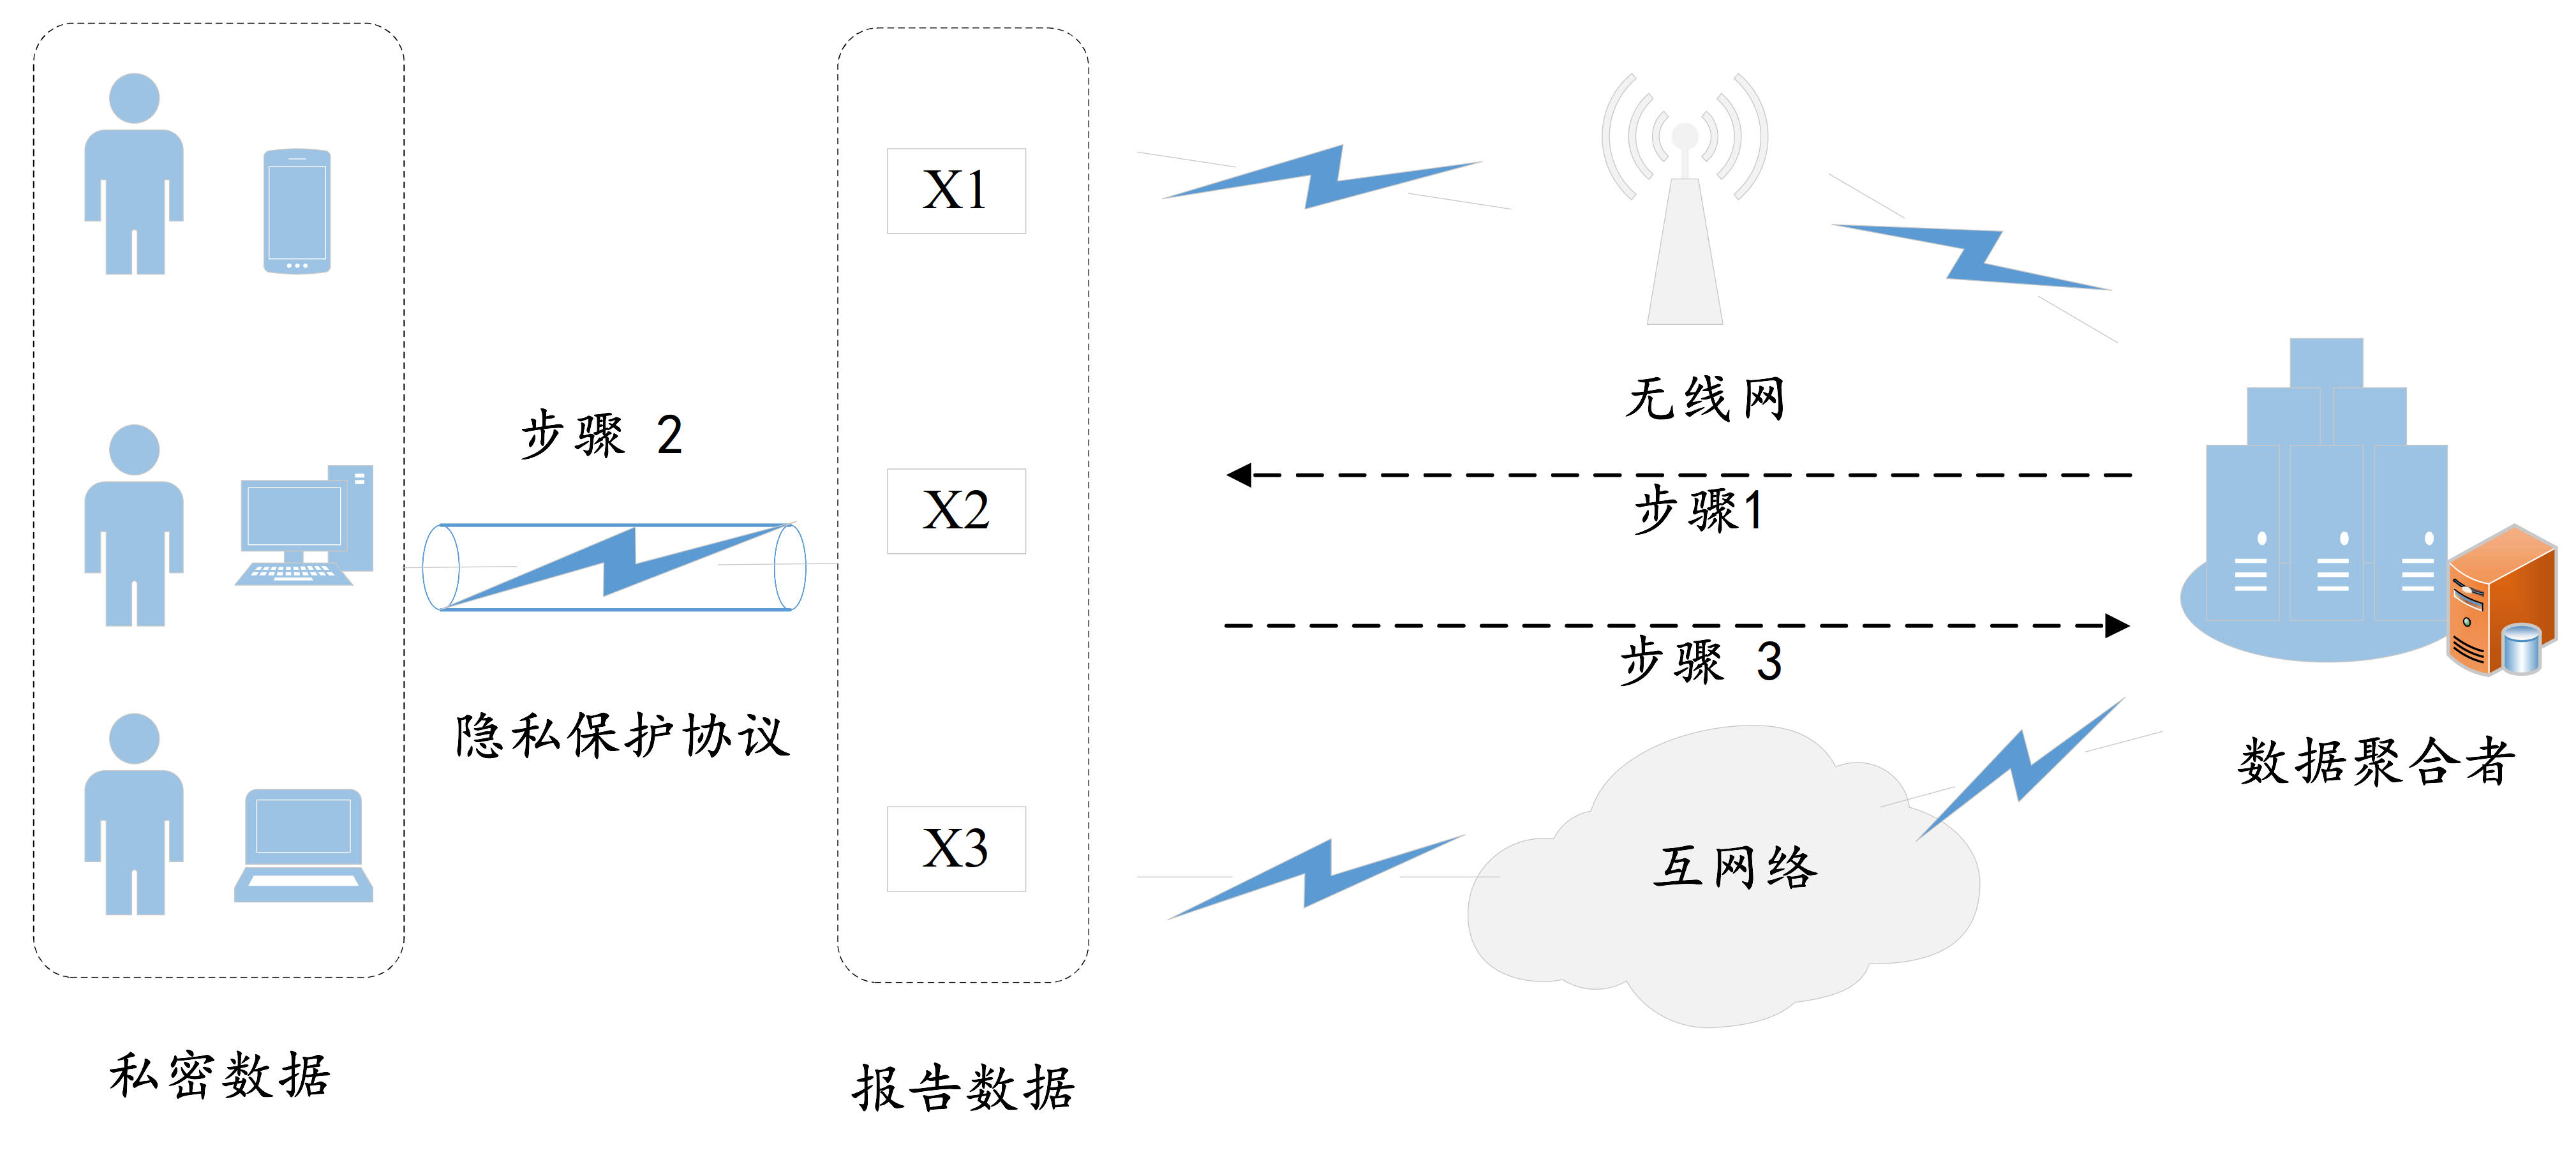
\includegraphics[width=5.5in,height=2.5in]{./figures/Application_architecture.jpg}
	\caption{隐私保护数据收集的系统模型}
	\label{Fig:chapter07_architecture}
\end{figure}

步骤1: 数据聚合者发布一个数据收集的信号,并决定收集数据的具体细节。这些将要被收集的数据可能包含个人的数据,如家庭地址、婚姻状态、性别、年龄等。然后,数据聚合者招募用户去上报她们自己的私密数据。

步骤2: 系统中的用户可以决定是否上报他们的数据给数据聚合者。如果一个用户同意参与到当前的数据收集任务,她将执行隐私保护协议得到伪装的数据,然后将得到的伪装数据上报给数据聚合者。

步骤3: 基于上述步骤1和步骤2,数据聚合者收集、存储用户的上报数据,然后分析这些上报的数据。


针对图~\ref{Fig:chapter07_architecture}描述的隐私保护数据收集系统模型,假设有$n$个用户参与,$[n]=\{1,2,\cdots,n\}$。有限集合$\mathcal{X}$和$\hat{\mathcal{X}}$分别表示用户数据和伪装数据的所有可能取值域,进一步,$|\mathcal{X}|$表示有限集合$\mathcal{X}$的不同原子数量,使用从$1$到$|\mathcal{X}|$的整数几个表示$\mathcal{X}$中真实字母表的序数。离散随机变量$X$和$\hat{X}$分别表示个人的原始数据和伪装数据。由此,LDP形成一个概率性函数,映射$x \in \mathcal{X}$到$\hat{x} \in \hat{\mathcal{X}}$的概率为$Q(\hat{x}|x)$,记作,$Q:\mathcal{X}\rightarrow \hat{\mathcal{X}}$。除此之外,本章中有时使用下标的$x_i$和$\hat{x}_i$表示第$i$个用户的数据和伪装数据。

为了保护用户个体的隐私信息,每个用户独立的扰动自己的原始数据得到扰动的数据,然后将扰动数据发送给数据聚合者。不失一般性,混淆机制与噪声信道相关,因为差分隐私的定义是基于一个随机的概率性函数。通过这种方式,LDP与信息论建立了基本的联系。为了更好的说明这种关系,以下给出一个具体的例子。

\begin{example}对于``是''和``否''的选择型问题,它可以被$\{0,1\}$二进制的候选集表示。对于这类问题,差分隐私的混淆机制可以被视为一个二元对称信道。例如,$Q_{0|0}=Q_{(1|1)}=0.7$和$Q_{010}=Q_{(0|1)}=0.3$,则其满足$\epsilon=\ln \frac{7}{3}$的$\epsilon$-差分隐私。
\end{example}

令$P$是支撑集$\mathcal{X}$上的任意一个概率分布,有限集合$\mathcal{P}$包含$\mathcal{X}$上所有可能的概率分布,则有$P\in \mathcal{P}$。 假设每一个用户的个人私密数据独立地抽样于的一个分布$P\in \mathcal{P}$,数据聚合者不知道这个分布$P$,仅知道它是集合$\mathcal{P}$的元素。基于这样的模型假定,本章中考虑策略型的敌手和数据聚合者知道彼此的策略空间。在这种情况下,聚合者旨在最大化隐私推断的成功概率。
\subsection{敌手模型}\label{adversary:model}

本章中,攻击模型是一个半诚实但好奇的(Semi-honest-but curious)敌手模型,也就是,数据聚合者诚实的执行隐私保护协议,但是试图从用户报告的扰动数据中去推断用户的个人隐私信息。事实上,聚合者可能是一个消息灵通的策略型敌手,他可能知道一些有关数据分布的先验知识帮助推断用户隐私。为了捕捉这个先验,假设聚合者仅知道数据分布属于一个确定的集合,$P\in \mathcal{P}$,但是不知道确切的数据分布$P$。在此情况下,本章中考虑一个策略型的敌手$A$,他知道用户的隐私保护策略集$\mathcal{Q}$,并有一些数据分布的先验知识$\mathcal{P}$,目标是获取最大的隐私信息量以保证能够推断、识别用户的真实隐私信息。

\subsection{问题提出}\label{sec:chapter06-problem}
差分隐私的预算参数$\epsilon$是量化隐私保护不可区分等级的事实标准,但是,$\epsilon$-度量提供了最差情况下的隐私保证,那也就是说,这个度量是对隐私攻击者有一个较强的假设。因为$\epsilon$-度量仅依赖于概率性映射函数,如引言中所述的这个度量存在着一些不足之处\cite{lopuhaa-zwakenberg2019information}。如果存在一个隐私保护机制集合$\mathcal{Q}$,集合中的每个元素$Q\in \mathcal{Q}$都提供$\epsilon$-隐私保障,则$\epsilon$-度量无法区分哪一个机制具有较好的隐私保护效果。然而,在很多的应用中,这些隐私保护机制的质量又迫切需要评估。针对这个问题,信息论方法提供了一种有效的解决途径,以下从定义开始介绍其方法的具体细节。

\begin{definition}\label{def:equivalent_privacy_mechanism}离散有限集合$\mathcal{Q}$表示一个含有$k$个隐私保护机制的集合。如果$\mathcal{Q}$中的每一个机制$Q^i:\mathcal{X}\rightarrow\hat{\mathcal{X}}$(s.t.$1\leq i \leq k$)是一个$\epsilon$-隐私机制,则这些机制$\{Q^i\}_{i=1}^{k}$称为一个等价$\epsilon$-隐私机制。
	
\end{definition}
\begin{remark}{\em 上述定义}\ref{def:equivalent_privacy_mechanism}{\em 可以被放松获得一个宽松的LDP机制集合,也就是,一个任意的隐私机制$Q^i \in \mathcal{Q}$是$\epsilon_i$-LDP机制。}
\end{remark}


事实上,隐私保护机制$Q^i:\mathcal{X}\rightarrow\hat{\mathcal{X}}$是一个损失压缩机制,它控制着从原始数据到伪装数据的隐私信息比特流动。为了量化信息的流动量,使用信息论的方法定义聚合者的信息增益为
\begin{definition}\label{def:information_gain}
	对于给定的隐私信息$x_i$,概率分布$P(X=x_i)$和$P(X=x_i|\hat{X}=\hat{x}_i)$分别表示先验分布和观察到$\hat{x}_i$后的后验概率分布。概率分布的比值$\log\left(\frac{P(X=x_i|\hat{X}=\hat{x}_i)}{P(X=x_i)}\right)$定义为聚合者的信息增益。
\end{definition}

基于上述定义\ref{def:information_gain},可以在观察到扰动数据之后,测量有关原始数据的不确定度减少量。本质上,这个度量是关于原始数据的先验和后验概率分布的比较。此外,注意到这个度量和信息论中著名的互信息具有相同的形式。重要地,期望形式的互信息测量一个用户的平均信息损失量,可以用来测量隐私机制的隐私泄露量,也就是互信息泄露
\begin{equation}
	I(X;\hat{X})=\sum_{x\in\mathcal{X}}\sum_{y\in\hat{\mathcal{X}}}P(x)Q(\hat{x}|x)\log\left(\frac{Q(\hat{x}|x)}{P(y)}\right)
\end{equation}
基于互信息隐私泄露的概念,等价的$\epsilon$隐私机制之间是彼此可以比较的。为了阐述一个偏序关系,首先给出以下定义
\begin{definition}
	对于一个给定的先验概率分布$P$,和任意的两个隐私机制$Q^i,Q^j\in \mathcal{Q}$(s.t.$1\leq i,j\leq k$)。如果$I(P;Q^i)\leq I(P;Q^j)$,则有$Q^i\succcurlyeq Q^j$;否则,$Q^i \prec Q^j$。
\end{definition}

具体的来说,这种偏序关系是可以传递的,它可以用来比较不同机制的隐私保护强度。接下来,考虑互信息测量隐私泄露。首先,互信息测量的隐私泄露聚焦在测量给定伪装数据时,原始数据的不确定度。其次,伪装数据在满足差分隐私的同时应该保持有关原始数据的信息内容尽可能的多。进一步,伪装数据包含的信息量由著名的互信息测量。基于这些理论上的支撑,本章考虑理性的用户旨在减少原始数据与伪装数据之间的互信息量,以至于聚合者不能拥有足够的信息完全识别一个用户的个人数据。然而,理性的聚合者想要去最大化隐私泄露去得到更多的隐私信息。基于这样的分析,用户的隐私目标可以形式化表述为下列的极小极大问题,则有
\begin{equation}
	\inf_{Q\in \mathcal{Q}}\sup_{P\in \mathcal{P}}I(P;Q)
\end{equation}

另外,聚合者想要估计一个分布最大化互信息泄露,因为一个先验的概率分布集合对聚合者是可见的。在这种情况下,隐私机制在最差情况下的互信息泄露将会是
\begin{equation}
	\sup_{P\in \mathcal{P}}\inf_{Q\in \mathcal{Q}}I(P;Q)
\end{equation}
事实上,上面的问题被建模成为一个极小极大的问题,它变成了一个凸优化问题\cite{boyd2004convex}。极小极大的问题捕捉到一个基本的场景,参与者的目标是相对立的。在实践中,聚合者可能是一个策略型的参与者而不仅仅受限于仅能观察伪装数据,他可以适应性的改变他自己的策略根据用户的保护策略。在这样的情况下,本章中考虑互信息泄露作为聚合者的信息增益。

\section{隐私保护攻防博弈}\label{sec:chapter06-PPAD}
本节中针对上述\ref{sec:chapter06-problem}小节提出的极大极小隐私问题,给出隐私保护的攻防博弈模型(PPAD),并进行相应的均衡分析。
\subsection{博弈模型}\label{subsec:chapter06-gamemodel}
上述隐私保护数据收集的系统模型中,每一个用户使用隐私保护机制扰动自己的原始数据,类似于隐私防护者。同样地,不可信的数据聚合者试图推断用户隐私信息类似于一个隐私攻击者。基于这样的类比,上述\ref{sec:chapter06-problem}小节的极小极大隐私问题自然地演变为一个隐私攻击和防御的对策博弈问题。为了有一个较好的阐述,下面首先给出隐私攻防博弈的定义。

\begin{definition}\label{def:PPAD}隐私保护的攻防博弈(PPAD)框架是一个元组$(D,A,\mathcal{D},\mathcal{A},U)$,其中,有限集合$\mathcal{D}$和$\mathcal{A}$分别是隐私保护者$D$和隐私攻击者$A$的策略空间,$U:\mathcal{D}\times \mathcal{A}\rightarrow\mathbb{R}$是冯诺依曼$\cdot$摩根斯坦(von Neumann-Morgenstern)效用函数。由此,隐私防护者和攻击者的理性行为可以被定义为
	\begin{equation}
		\begin{cases}
			s_{d}^{*} \overset{\text{def}}{=} \arg \min_{s_{d}\in \mathcal{D}}U_{D}(s_{d},s_{a}^{*})\\
			s_{a}^{*} \overset{\text{def}}{=} \arg \max_{s_{a}\in \mathcal{A}}U_{A}(s_{d}^{*},s_{a}).
		\end{cases}
	\end{equation}
\end{definition}

%上述定义\ref{def:PPAD},给出了一个标准形式的攻防博弈描述。



{\em 为了阐述更多的细节,以下给出隐私保护的攻防博弈$(D,A,\mathcal{D},\mathcal{A},U)$的标准形式描述,包括博弈参与者、参与者策略空间和效用函数。具体如下:
	\begin{itemize}
	\item 攻防博弈的参与者包括防护者(\underline{D}efender)和攻击者(\underline{A}ttacker),则有,参与者$=\{D,A\}$;
	
	\item 有限集合$\mathcal{D}$和$\mathcal{A}$分别为$D$和$A$的策略空间,其中,所有可行的隐私机制集合$\mathcal{Q}$是防护者的策略空间,即$\mathcal{D} \triangleq \mathcal{Q}$; 此外,所有可能的概率分布集合$\mathcal{P}$是攻击者的策略空间,即$\mathcal{A} \triangleq \mathcal{P}$;
	
	\item 博弈参与者$D$和$A$的收益函数$U(P,Q)$采用互信息度量,对于任意的$P \in \mathcal{P}$和$Q \in \mathcal{Q}$,参与者的收益计算依据下式效用函数$U(P,Q)$
	\begin{equation} \label{eq:MI}
		U(P,Q)= \sum_{\mathcal{X}}\sum_{\mathcal{\mathcal{Y}}}P^{T}Q\log \left(\frac{Q}{\sum_{\mathcal{X}}P^{T}Q}\right)
	\end{equation}
	\end{itemize}

}

\begin{example}\label{exam:chapter7_02}假设信源概率分布集合$\mathcal{P}$包含$3$个不同的分布,字母表$|\mathcal{X}|=3$,记作$P^i \in \mathcal{P}, i \in \{1,2,3\}$。具体的实例如下表\ref{tab:chapter7_2}所示。

\begin{table}[!ht]
	%\scriptsize
\small
	\centering
	\caption{数据概率分布示例}
	\label{tab:chapter7_2}\centering
	\begin{tabular}{p{1.2cm}p{1.8cm}p{1.8cm}p{1.8cm}}
		\hline\noalign{\smallskip}
		& $p_{(1)}$ & $p_{(2)}$ & $p_{(3)}$  \\
		\noalign{\smallskip}\hline\noalign{\smallskip}
		$P^{1}$ & 0.25 & 0.35 &0.4\\
		$P^{2}$ & 0.35 & 0.5  &0.15\\
		$P^{3}$ & 0.6 & 0.2  &0.2\\
		\noalign{\smallskip}\hline
	\end{tabular}
\end{table}

更多的,一个隐私机制的集合$\mathcal{Q}$包含有$3$个不同隐私机制,记作$\mathcal{Q}=\{Q^1,Q^2,Q^3\}$,更多的细节如表\ref{tab:chapter7_mechanisms}所示。如此以来,本例表述的隐私保护攻防博弈是一个二人矩阵博弈的实例。

\begin{table}[!htb]
%\scriptsize
\small
\centering
\caption{$\epsilon=\ln2$的隐私机制}
\label{tab:chapter7_mechanisms}
\begin{tabular}{cccccccccc}
\toprule
\multirow{2}{*}{$\mathcal{Q}$} & \multicolumn{3}{c}{$Q^1_{(y|x)}$} & \multicolumn{3}{c}{$Q^2_{(y|x)}$} & \multicolumn{3}{c}{$Q^3_{(y|x)}$} \\
\cmidrule(r){2-4} \cmidrule(r){5-7} \cmidrule(r){8-10}
&  $1$      &  $2$   &   $3$
&  $1$      &  $2$   &   $3$
&  $1$      &  $2$   &   $3$ \\
\midrule
$1$  &0.4  & 0.3 & 0.3   & 0.4  & 0.2   & 0.4  & 0.3    & 0.2   & 0.5  \\
$2$  &0.25   & 0.15  & 0.6 & 0.3  & 0.3  & 0.4  & 0.2  &0.4  & 0.4 \\
$3$ &0.2 & 0.2  & 0.6  & 0.2  & 0.4 & 0.4 & 0.15 & 0.35   & 0.5\\
\bottomrule
\end{tabular}
\end{table}
\end{example}

{\em 本章中所提出的隐私攻防博弈是一个有限策略的完全信息静态博弈(Simultaneous Games),意味着参与者$D$和$A$做出决策时不知道其它参与者的策略选择。此外,在攻防博弈PPAD中,参与者的策略行动$\mathcal{D},\mathcal{A}$和效用函数$U(\cdot,\cdot)$是隐私防护者$D$和攻击者$A$的共同知识(Common Knowledge)。在这种情况下,参与者被假设为理性的决策者,趋向于选择最大化自身收益的策略,基于此给出攻防博弈中参与者的理性行为分析。事实上,如果隐私攻击者收益等于防护者损失,则上述是二人零和博弈(Two-Person Zero-Sum,TPZS),其解是对策博弈的鞍点(Saddle Point,SD)。接下来,对所提出的攻防博弈PPAD进行均衡分析。}
\subsection{均衡分析}\label{subsec:chapter06-game-analysis}
针对本章中\ref{sec:chapter06-problem}小节形式化的极大极小问题,\ref{subsec:chapter06-gamemodel}小节提出了隐私保护的攻防博弈PPAD模型。针对上述博弈,本节中分析了博弈模型的效用函数性质、博弈的均衡,为在\ref{sec:chapter06-algorithm}节给出了博弈均衡的策略优化选择算法奠定理论基础。

首先,本文\ref{sec:chapter3_convex_concave_game}节介绍的凹凸对策博弈拥有一个特殊的效用函数形式,它是一个参与者策略的凸函数,同时也是另外一个参与者策略的凹函数\cite{washburn2014two}。在这样的博弈模型中,博弈的解是每个参与者的纯策略组合。本章中隐私攻防博弈的参与者策略集和效用函数满足凹凸性,为此给出以下分析。

\begin{lemma}\label{lem:chapter7_lemma01}对于任意的$\epsilon$-差分隐私$Q^1,Q^2 \in \mathcal{Q}$,一个实数$\alpha \in \mathbb{R}^+,0<\alpha<1$,它们的凸组合$Q^{\alpha}=\alpha Q^1+(1-\alpha)Q^2$仍然满足$\epsilon$-差分隐私。
\end{lemma}

{\em 证明:令$x_1,x_2$是两个任意的差分隐私输入数据,$\hat{x}$是一个任意的输出数据。则依据差分的定义,有下式成立
	\begin{alignat}{2}
	Q^{\alpha}(\hat{x}|x_1) & = \alpha Q^1(\hat{x}|x_1)+(1-\alpha)Q^2(\hat{x}|x^2)\\
	& \leq \alpha Q^1(\hat{x}|x_2)\cdot \exp(\epsilon)+(1-\alpha)Q^2(\hat{x}|x^2)\cdot \exp(\epsilon)\\
	& = \exp(\epsilon)\cdot Q^{\alpha}(\hat{x}|x_2) \label{eq:chapter7_2.8}
	\end{alignat}
上述公式\ref{eq:chapter7_2.8}满足差分隐私定义,故有$Q^\alpha$仍然是$\epsilon$-差分隐私。
}


上述$\epsilon$-隐私机制的性质已在相关研究工作中使用\cite{kalantari2018robust}。对于本章中所提出的隐私保护攻防博弈模型,攻击者和防护者的策略都是概率分布集合,假设它们是凸集。基于文献\mycite{cover2006elements}中的定理2.7.4,则有,对于任意的$Q$,收益函数$U(P,Q)$满足一个封闭凸集的凹函数,同时,对于每一个$P$,收益函数$U(P,Q)$是$Q$的凸函数。这是由于互信息函数的凹凸性(定理2.7.4\cite{cover2006elements}的证明),基于这个理论分析的结果,所提出的隐私保护攻防博弈(PPAD)模型是一个凹凸博弈。


其次,均衡分析是对策博弈论中的一个重要研究课题,它的目标是寻找对策博弈模型的解。博弈均衡\cite{Neumann1944The}是一种稳定的状态,该状态下没有参与者有动机改变他当前的策略以获得更大的收益。对于所提出的隐私攻防博弈PPAD模型,结合凹凸博弈的性质给出以下具体的博弈均衡分析。

\begin{lemma} \label{lemma:chapter07_01}
	如果$U:\mathcal{P}\times \mathcal{Q}\rightarrow\mathbb{R}$是$P$的一个凹函数,则攻击者有最佳的响应策略满足$\max_{P\in \mathcal{P}}\min_{Q \in \mathcal{Q}}U(P,Q)$。相似的,如果它是$Q$的一个凸函数,则防护者有最佳响应策略满足$\min_{Q \in \mathcal{Q}}\max_{P \in \mathcal{P}}U(P,Q)$。
\end{lemma}

{\em 上述引理\textup{\ref{lemma:chapter07_01}}的证明过程类似于文献\textup{\mycite{washburn2014two}}中对于定理\textup{5.2}的证明,此处省略去其具体证明过程。
}
\begin{remark}{\em
如果隐私防护者首先选择行动策略,攻击者随后选择策略行动。则有,防护者希望极小化支付量$U(P,Q)$,因此选择$Q \in \mathcal{Q}$极小化$U(P,Q)$,获得$\inf _{Q \in \mathcal{Q}}U(P,Q)$。攻击者选择$P \in \mathcal{P}$使得最坏情况下的支付最大化,攻击者选择$\arg\max_{P\in \mathcal{P}}U(P,Q)$,期望获得支付量$\sup_{P\in\mathcal{P}}\inf_{Q \in \mathcal{Q}}U(P,Q)$。如果和上述策略选择行动顺序相反,防护者可以获得$\inf_{Q \in \mathcal{Q}}\sup_{P\in \mathcal{P}}U(P,Q)$。
}
\end{remark}

除了上面提到的,所提出的隐私保护攻防博弈PPAD模型属于完全信息的静态博弈研究范畴,每一个参与者可以预测其它参与者的最佳响应策略,也就是最优策略。作为一个结果,无论一个攻击者还是防护者都会对其它参与者的策略选择有一个最佳响应策略。基于这个结果,则有下面的定理。

\begin{theorem}\label{theorem:chapter07_02}
对于有限概率分布集合$\mathcal{P}$和$\mathcal{Q}$,隐私保护的攻防博弈存在一个鞍点$(P^*,Q^*)$满足$U(P,Q^*)\leq U(P^*,Q^*)\leq U(P^*,Q)$ 对所有的$P\in \mathcal{P}$和$Q \in \mathcal{Q}$。
\end{theorem}
{\em 证明:对于任意的$Q^1,Q^2 \in \mathcal{Q}$,和一个参数$\alpha \in \mathcal{R}^+$($0 <\alpha < 1$),它们的凸组合$Q^{\alpha}=\alpha Q^1+(1-\alpha)Q^2$仍然是$\epsilon$-差分隐私。因为$\mathcal{P}$和$\mathcal{Q}$都是概率分布集合,是欧几里德空间的凸子集。进一步,$U(P,Q)$是一个有关$P$和$Q$的二元函数,关于$P$的凹函数,关于$Q$的凸函数。更重要的是有限集合$\mathcal{P}$和$\mathcal{Q}$是紧致的,即封闭有界集合。然后,基于著名的极大极小定理\textup{\ref{theorem:minmax}}
,隐私保护的攻防博弈PPAD存在鞍点$(P^*,Q^*)$满足$U(P,Q^*)\leq U(P^*,Q^*)\leq U(P^*,Q)$。
}
\begin{corollary}对所有的$P\in \mathcal{P}$和$Q \in \mathcal{Q}$,策略组合$(P^*,Q^*)$满足
\begin{equation}\label{eq:saddle point}
	\begin{cases}
		U(P^*,Q^*) = \sup_{P\in\mathcal{P}}U(P,Q^*)\\
		U(P^*,Q^*) = \inf_{Q\in\mathcal{Q}}U(P^*,Q).
	\end{cases}
\end{equation}
则$(P^*,Q^*)$称为函数$U(P,Q)$ 在乘积空间$\mathcal{P}\times\mathcal{Q}$的鞍点。
\end{corollary}
从上述定理\ref{theorem:chapter07_02}可以看出,隐私保护攻防博弈PPAD的鞍点$(P^*,Q^*)$是隐私保护系统模型中隐私信息泄露的一个极端状态,从隐私泄露量的角度对于隐私防护者的隐私信息保护是一种最差的情况。此外,推论中公式\ref{eq:saddle point}表明鞍点$(P^*,Q^*)$的支付量$U(P^*,Q^*)$是隐私攻击者可以从原始数据中获取的最小隐私信息增益。同时,这个支付量是防护者最大可能的信息损失。基于鞍点的内涵,隐私保护攻防博弈的鞍点支付量可以用来评估互信息隐私泄露。事实上,这个支付量是互信息隐私泄露的上界。

\section{策略优化选择算法}\label{sec:chapter06-algorithm}
上述\ref{subsec:chapter06-game-analysis}小节针对提出的隐私攻防博弈给出了均衡分析,接下来,介绍隐私保护策略优化选择算法。首先,基于上述引理\ref{lemma:chapter07_01},鞍点策略$(P^*,Q^*)$是每一个参与者的最佳响应策略。事实上,提出的隐私保护攻防博弈是一个有限策略的二人零和对策博弈,并结合参与者效用函数的凹凸性,基于定理\ref{theorem:chapter07_02}分析了鞍点的存在性。其次,在解博弈模型的过程中,对于鞍点的计算是两个凸集之间的一个交替最优化问题。基于最优响应策略思想,设计一个计算攻防博弈鞍点的策略优化选择算法,用于解决最初给出的隐私泄露极小极大问题。最后,算法计算是一个交替最优化的过程,该过程类似于两个凸集之间最小化距离的解决方法。具体的,策略优化选择算法的计算过程主要包含有以下三个步骤。

步骤1:初始化选择一个任意防护者策略$Q \in \mathcal{Q}$,攻击者计算一个最优的响应策略$P$,即是$\arg \max_{P \in \mathcal{P}}U(P,Q)$。

步骤2:防护者预测攻击者的策略偏好,由此,防护者将会采用使得收益最大化的策略,也即是$\arg \min_{Q \in \mathcal{Q}}\max_{P \in \mathcal{P}}U(P,Q)$。

步骤3:交替最优化处理、更新参与者的策略选择,并重复上述步骤直到一个策略组合$(P^*,Q^*)$对隐私攻击者和防护者都是最优的。

\begin{algorithm}[htbp]
    \small
    \setstretch{1.2}
	\caption{隐私攻防博弈的策略优化选择算法}
	\label{alg:game}
	\begin{algorithmic}[1]
		\REQUIRE ~~\\
            \begin{tabular}[t]{p{8mm}l}
            $\mathcal{P}$&:攻击者$A$的可行策略空间\\
            $\mathcal{Q}$&:防护者$D$的可行策略集合\\
            $U(P,Q)$&:效用函数
            \end{tabular}
		\ENSURE ~~\\
            \begin{tabular}[t]{p{8mm}l}
            $(P^*,Q^*)$&:鞍点策略\\
            $SD$&:鞍点策略的支付量
            \end{tabular}
		\STATE 初始化集合$S_1 \leftarrow Q^0$使用一个任意的策略$Q^0 \in \mathcal{Q}$
		\STATE 计算攻击者的一个最优响应策略$P^* = \arg \max_{P\in \mathcal{P}}U(P,Q^0)$
		\STATE 计算防护者的最优反应策略$Q^* = \argmin_{Q \in \mathcal{Q}}U(P^*,Q)$
		\WHILE{($P^*,Q^*$)不是博弈鞍点}
		\STATE 计算攻击者最优响应策略$P^* = \arg \max_{P\in \mathcal{P}}U(P,Q^*)$
		并更新 $P^*$ 重新计算 $U(P^*,Q^*)$ 利用公式\ref{eq:MI}
		\IF{$(P^*,Q^*)$ 是博弈鞍点}
		\RETURN $(P^*,Q^*)$ 和 $SD \leftarrow U(P^*,Q^*)$
		\ELSE
		\STATE 计算防护者最优响应策略 $Q^*=\argmin_{Q \in \mathcal{Q}\setminus S_1}U(P^*,Q)$\\
		和 $U(P^*,Q^*)$ 使用公式\ref{eq:MI}
		\STATE 更新集合 $S_1 \leftarrow S_1 \bigcup Q^*$
		\ENDIF
		\ENDWHILE
	\end{algorithmic}
\end{algorithm}

上述算法\ref{alg:game}描述了策略优化选择的具体计算过程,算法接受输入攻防博弈的结构,也即是博弈规则,包括参与者的策略空间$\mathcal{P},\mathcal{Q}$和效用函数$U(P,Q)$。然后,算法执行计算过程并输出博弈鞍点$(P^*,Q^*)$和支付量$SD$。首先,算法初始化一个任意的策略$Q^0 \in \mathcal{Q}$,并为$Q^0$计算一个最优的响应策略$P^*$(算法的$1 \sim 2$行)。其次,算法计算隐私防护者的一个最优响应策略$Q^*$,用来防护攻击者的策略$P^*$(算法的第$3$行)。进一步,算法重复执行上面的这些交替最优化的步骤,直到一个稳定的状态$(P^*,Q^*)$对于攻击者和防护者都是最优的响应策略(算法的$4 \sim 12$行)。最后,算法返回博弈的鞍点策略及其对应的支付量。

为了直观地理解上述算法的过程,利用例子\ref{exam:chapter7_02}给出具体的解释说明,支付矩阵如表\ref{tab:chapter07_payoff}所示。为了说明算法\ref{alg:game}的计算步骤,假设防护者首先选择策略$Q^1$,然后攻击者偏好于采取$P^3$策略,目的是为了获得一个最大的支付量$0.0662$,也就是说,$P^3$ 是攻击者对$Q^1$的最优响应策略。进一步,防护者可以预测攻击者的行动$P^3$,并使用策略$Q^2$去最小化隐私损失,即是,防护者期望获得$0.0315$的收益。因此,$Q^2$是防护者对攻击策略$P^3$的最优响应。同时,$P^3$也是攻击者对防护者策略$Q^2$的最优响应。所以,策略组合$(P^3,Q^2)$是隐私攻防博弈的鞍点,具有支付量$0.0315$。而且,鞍点策略提供$\epsilon=\ln 2$的$\epsilon$-差分隐私。对此,图\ref{fig:chapter07_rational}清晰的描绘了参与者的理性决策过程。
\newline

\makeatletter\def\@captype{table}\makeatother
\begin{minipage}{.99\textwidth}
	\centering  \caption{对策博弈的支付矩阵} \label{tab:chapter07_payoff}
	\begin{blockarray}{ccccc}
		& $Q^{1}$& $Q^{2}$&$Q^{3}$&\\
		\begin{block}{c[ccc]c}
			$P^1$ &0.0531	&0.0308  &	0.0299	& $.0299$\\
			$P^2$& 0.0627	&0.0226	 &  0.0339 & $.0226$\\
			$P^3$& 0.0662	&0.0315	 &  0.0345 & $.0315$\\
		\end{block}
		& $.0662$& $.0315$&$.0345$&
	\end{blockarray}\\
\end{minipage}

\begin{figure}[!ht]
	\centering 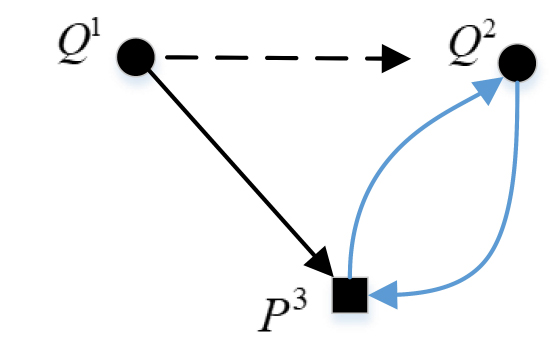
\includegraphics[width=2.0in,height=1.2in]{./figures/decision.jpg}
	\caption{理性决策过程的描述说明}
	\label{fig:chapter07_rational}
\end{figure}

{\em 通过分析算法\textup{\ref{alg:game}}的一些基本操作,给出计算博弈鞍点的计算复杂度。首先,算法在第一轮迭代中搜索攻击者的策略空间$\mathcal{P}$,寻找一个最优的响应策略$P$。其次,针对攻击者策略算法计算一个最优响应策略$Q$,需要搜索防护者的策略空间$\mathcal{Q}$。最后,算法的终止条件保证了极大极小问题的解。鉴于上述分析可知,计算开销随着$\mathcal{P}$和$\mathcal{Q}$的大小而变化。只要策略集合$\mathcal{P}$和$\mathcal{Q}$是有限的,算法计算过程是有效的。
}
\section{实验与分析}\label{sec:chapter06-experiment}
本节中给出所提出隐私保护策略选择方案的实验结果,并给出实验结果的分析。基于Java实现本章中伪代码描述的算法,并部署在安装Windows 10操作系统的个人PC上执行实验程序。实验分析有两个部分组成,首先,\ref{sec:case_study}节给出一个具体的实例分析,随后,\ref{sec_numberic_simulation}节给出数值实验分析结果。
\subsection{实例分析}\label{sec:case_study}

对于字母表$|\mathcal{X}| = |\hat{\mathcal{X}}|=6$的情况,本章假设数据先验分布属于一个确定的概率分布集合,但是不能精确的知道真实的数据分布。为了有一个直观的说明,本章借用文献\mycite{kalantari2018robust}中的分布数据,并在表\ref{tab:chapter07_5}中给出它们的分布律。

\begin{table}[!ht]
	%\scriptsize
    \small
	\caption{$|\mathcal{X}|=6$的概率分布}
	\label{tab:chapter07_5} \centering
	\begin{tabular}{p{1cm}p{1cm}p{1cm}p{1cm}p{1cm}p{1cm}p{1cm}}
		\hline\noalign{\smallskip}
		& $p_{(1)}$ & $p_{(2)}$ & $p_{(3)}$  & $p_{(4)}$ & $p_{(5)}$ & $p_{(6)}$ \\
		\noalign{\smallskip}\hline\noalign{\smallskip}
		$P^{1}$ & 0.7 & 0.15 &0.06 & 0.04 & 0.03 &0.02\\
		$P^{2}$ & 0.15 & 0.7  &0.06 & 0.04 & 0.03  &0.02\\
		$P^{3}$ & 0.06 & 0.15  &0.7 & 0.04 & 0.03  &0.02\\
		$P^{4}$ & 0.04 & 0.15  &0.06 & 0.7 & 0.03  &0.02\\
		\noalign{\smallskip}\hline
	\end{tabular}
\end{table}
更多的,考虑两个等价可替换的$\epsilon=\ln 2$隐私机制,表\ref{tab:chapter07_6}给出两个隐私机制的条件概率分布,其中,$Q^1$是截断$\frac{1}{2}$- 几何机制\cite{ghosh2012universally},$Q^2$是文献\mycite{alvim2011differential}提出的隐私机制。进一步,考虑文献\mycite{kairouz2016extremal}中提出的著名$k$-RR机制,满足对角线概率$e^{\epsilon}/(|\mathcal{X}|-1+e^{\epsilon})$。基于此,$k$-RR提供$\epsilon=\ln 2$差分隐私保护,当且仅当概率密度函数$Q^3$满足
\begin{equation}\nonumber
	Q_{(y|x)}^3 = \begin{cases}
		\frac{e^{\epsilon}}{|\mathcal{X}|-1 +e^{\epsilon}} & \hat{x}=x\\
		\frac{1}{|\mathcal{X}|-1 +e^{\epsilon}} & \hat{x}\neq x
	\end{cases}
	\Rightarrow Q_{(y|x)}^3 = \begin{cases}
		2/7 & \hat{x}=x\\
		1/7 & \hat{x}\neq x
	\end{cases}
\end{equation}

\begin{table*}[htbp]
	%\scriptsize
\small
	\centering
	\caption{$|\mathcal{X}|=6$时提供$\epsilon=\ln2$的等价隐私机制}
	\label{tab:chapter07_6}
	\begin{tabular}{ccccccccccccc}
		\toprule
		\multirow{2}{*}{In/Out} & \multicolumn{6}{c}{$Q^1_{(y|x)}$} & \multicolumn{6}{c}{$Q^2_{(y|x)}$} \\
		\cmidrule(r){2-7} \cmidrule(r){8-13}
		&  $1$      &  $2$   &   $3$ &  $4$      &  $5$   &   $6$
		&  $1$      &  $2$   &   $3$ &  $4$      &  $5$   &   $6$\\
		\midrule
		$1$  &$2/3$  & $1/6$ &$1/12$   & $1/24$  & $1/48$   & $1/48$             &$4/11$  & $2/11$ &$1/11$ & $1/11$ &$1/11$  & $2/11$ \\
		$2$  &$1/3$   &$1/3$  & $1/6$ & $1/12$  & $1/24$  & $1/24$               &$2/11$  & $4/11$ &$2/11$ & $1/11$ &$1/11$  & $1/11$ \\
		$3$ &$1/6$ & $1/6$  & $1/3$  & $1/6$  & $1/12$ & $1/12$                  &$1/11$  & $2/11$ &$4/11$ & $2/11$ &$1/11$  & $1/11$ \\
		$4$ &$1/12$ & $1/12$  & $1/6$  & $1/3$  & $1/6$ & $1/6$                  &$1/11$  & $1/11$ &$2/11$ & $4/11$ &$2/11$  & $1/11$ \\
		$5$  &$1/24$ & $1/24$  & $1/12$  & $1/6$  & $1/3$ & $1/3$                &$1/11$  & $1/11$ &$1/11$ & $2/11$ &$4/11$  & $2/11$ \\
		$6$ &$1/48$ & $1/48$  & $1/24$  & $1/12$  & $1/6$ & $2/3$                &$2/11$  & $1/11$ &$1/11$ & $1/11$ &$2/11$  & $4/11$ \\
		\bottomrule
	\end{tabular}
\end{table*}

上述隐私机制$\{Q^1,Q^2,Q^3\}$是等价的$\ln 2$-隐私机制。为了对这些隐私机制进行比较,假设它们是隐私防护者的所有可能策略。基于这个假设,在此给出以下分析。

基于上述的这些参与者可选行动策略,分析隐私攻击者和防护者的理性策略行为。通过算法\ref{alg:game}求解所对应的博弈模型。作为博弈的解,算法输出一个鞍点$P^1,Q^3$ 和支付量$0.0351$,这个结果意味着互信息隐私泄露将不会超过一个界($0.0351$)。在其它策略组合情况下,隐私防护者将会有动机改变他当前的隐私保护策略。例如,当考虑均匀的先验概率分布,对策博弈的支付量将会是$0.0633$。综合上述情况,这些情况意味着最佳的隐私保护机制和先验分布密切相关。

此外,本章还利用信息论度量方法解决了等价隐私保护机制之间无法比较的问题。例如,考虑均匀的先验概率分布情景,这些隐私机制的互信息隐私泄露是严格有序的,即$Q^1=0.5074 > Q^2=0.2164>Q^3=0.0633$。事实上,互信息隐私泄露的这些数值表达出了隐私防护者对于不同博弈产出的偏好。由此,则可以得到$Q^3 \succ Q^2 \succ Q^1$。这种严格的偏序关系对等价的隐私保护机制提供了一种有效的评估方法。


\subsection{数值分析}\label{sec_numberic_simulation}
为了获得数值实验结果,本文中分别对$|\mathcal{X}|=6$和$|\mathcal{X}=12|$随机的生成$10$个不同的分布。然后,利用随机化响应技术实现隐私保护机制。参考文献\mycite{kairouz2016extremal},实验中设置$\epsilon$参数在$0$到$10$的区间变化,如此可以获得一个隐私保护机制的集合。基于这些随机的数值数据,给出下面的实验分析。

数据先验概率分布和随机生成的不同隐私机制分别为隐私攻击者和隐私防护者的可用策略行动,并在这些数据上执行实验,利用所提出的策略优化选择算法\ref{alg:game}计算隐私保护攻防博弈的鞍点。为了克服随机性的影响,实验中通过归一化的互信息$I(X;\hat{X}/H(X))$比较所有隐私机制的平均性能,也即是隐私支付量。在所提出的隐私攻防博弈模型中,理性的隐私攻击者和隐私防护者偏好于采用获得最大化(最小化)博弈支付的策略。事实上,互信息隐私泄露是隐私预算$\epsilon$的严格单调函数,由此,随着$\epsilon$的增加,归一化的互信息隐私泄露曲线可以被描绘出来。

\begin{figure}[htbp]
\centering
\begin{minipage}[t]{0.48\textwidth}
\centering
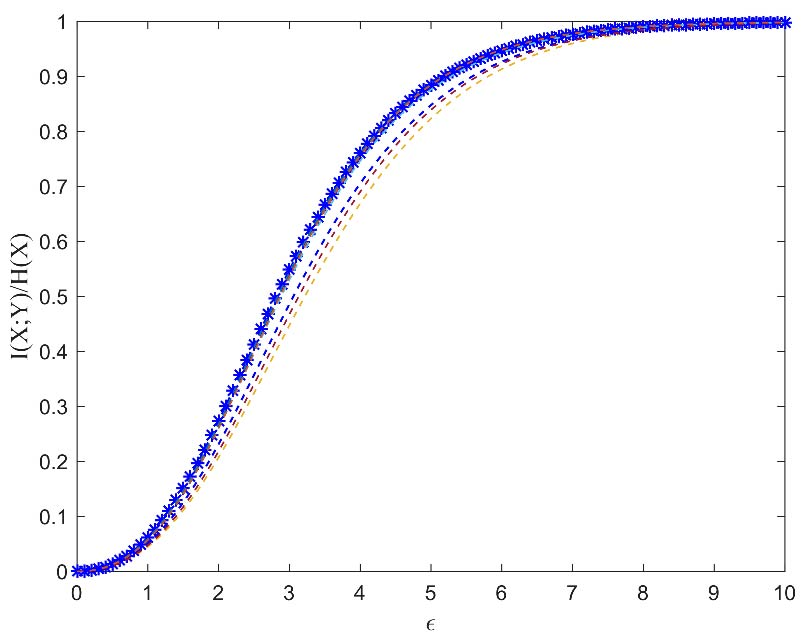
\includegraphics[width=7cm,height=2.0in]{./figures/Fig3.jpg}
\caption{$|\mathcal{X}|=6$时$I(X;\hat{X})/H(X)$}
\label{Fig:chapter06-3}
\end{minipage}
\begin{minipage}[t]{0.48\textwidth}
\centering
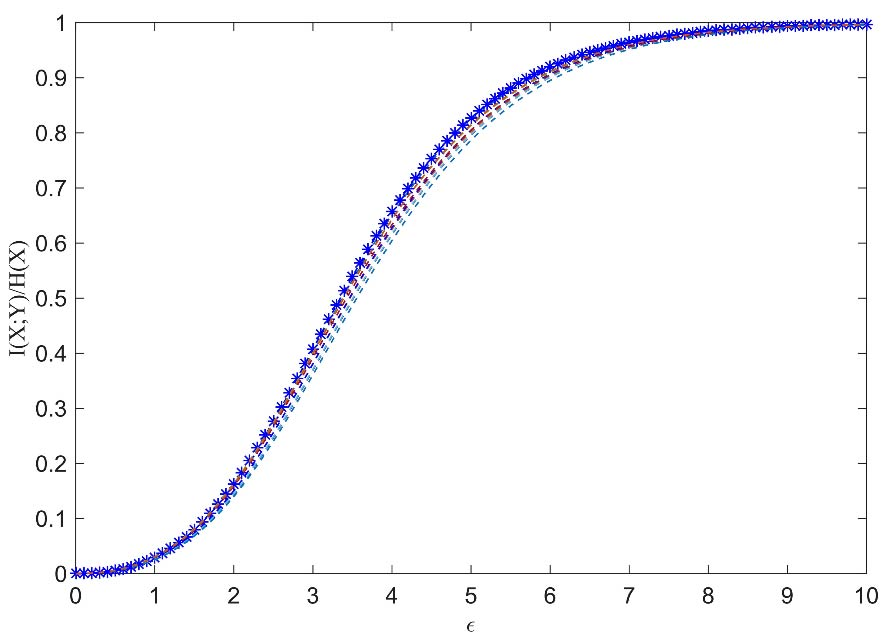
\includegraphics[width=7cm,height=2.0in]{./figures/Fig4.jpg}
\caption{$|\mathcal{X}|=12$时$I(X;\hat{X})/H(X)$}
\label{Fig:chapter06-4}
\end{minipage}
\end{figure}

%\begin{figure*}[htbp]
%	\centering
%		\begin{minipage}[t]{7cm}
%			\centering
%			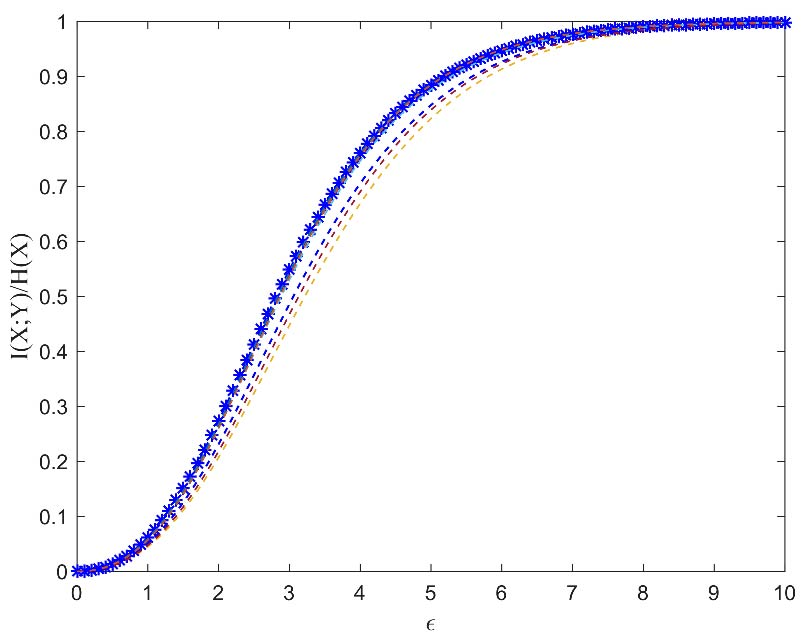
\includegraphics[width=2.5in,height=2.0in]{./figures/Fig3.jpg}
%			\label{Fig:3a}
%		\end{minipage}
%		\begin{minipage}[t]{7cm}
%			\centering
%			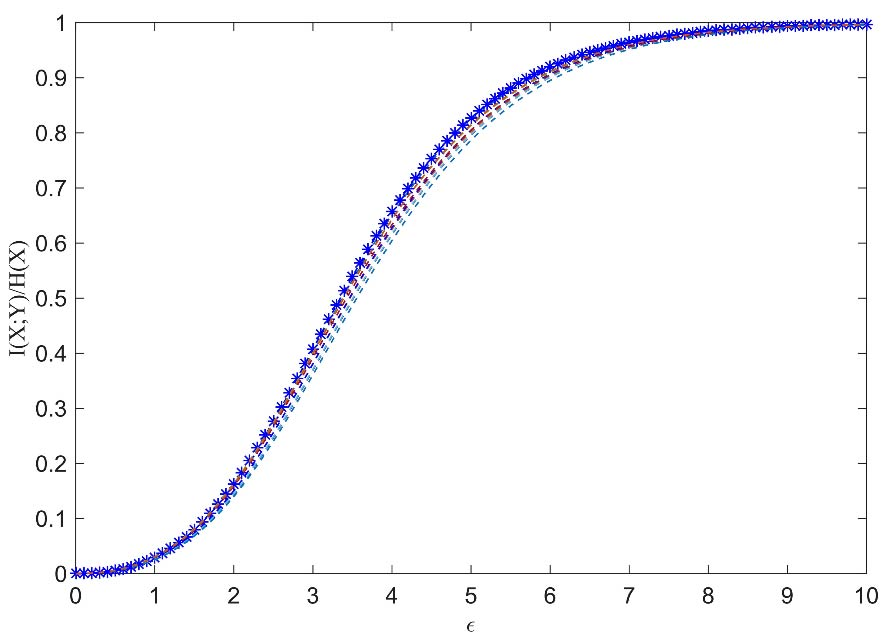
\includegraphics[width=2.5in,height=2.0in]{./figures/Fig4.jpg}
%			\label{Fig:3b}
%		\end{minipage}
%	\centering
%	\caption{隐私机制的归一化$I(X;\hat{X})/H(X)$ 对于随机生成的$10$个分布}
%	\label{fig:numerical simulation}
%\end{figure*}
图~\ref{Fig:chapter06-3}和图~\ref{Fig:chapter06-4}给出了数值实验结果。从图中可以看出,鞍点策略的互信息隐私泄露对于隐私防护者是最差情况的隐私泄露。另外,图~\ref{Fig:chapter06-3}和图~\ref{Fig:chapter06-4}还表明了上述结论对于字母表基数$|\mathcal{X}|$是不敏感的,因为两组实验具有相同的趋势。最差情况下的互信息隐私泄露可以帮助评估隐私泄露风险,选择适当的$\epsilon$参数在隐私容忍的范围内。

\section{本章小结}\label{sec:chapter06-conclusion}

本章针对差分隐私数据收集应用中存在的策略型攻击问题,利用信息论、博弈均衡理论研究了隐私防护者与隐私攻击者的理性策略选择,提出了隐私保护的攻防博弈(PPAD)模型,以实现隐私与数据效用均衡。首先,基于信息论度量方法分析差分隐私保护系统中隐私保护者和攻击者的隐私目标,形式化表述为互信息隐私的极大极小问题。其次,针对上述提出的问题,考虑策略型的隐私攻击者和防护者,提出隐私保护的攻防博弈模型,并具体为二人的零和博弈模型。随后,给出博弈的凹凸性以及均衡分析。进一步,为了求解博弈模型鞍点,设计了策略优化选择算法。最后,通过实验阐述了所提出的方案可以用于比较等价的隐私机制,并阐述了隐私量化是最坏情况下的隐私泄露,也即是,隐私防护者的最大隐私泄露。
 %实验结果展示
\chapter{总结与展望}\label{chapter09}
{\em 本章首先总结文中针对$\CTL$和$\mu$-演算下的遗忘理论做出的研究工作,概括文中使用的方法及取得的研究成果。其次,讨论分析本文工作中存在的不足之处,并基于此对本文的后续研究内容进行了展望。}

\section{工作总结}
随着计算机系统日益变得复杂,描述系统规范的语言也变得越来越复杂。随着信息的更新,系统的规范也随着改变,因而急需有效的方法来提取相关原子命题下的知识。
遗忘是一种知识提取的方法,本文从语法和语义的角度探索了广泛应用于并行系统的$\CTL$下的遗忘。此外,也探索了表达能力更强的$\mu$-演算下的遗忘。
具体地,本文的主要工作总结如下:

(1) 从语义的角度给出了$\CTL$和$\mu$-演算下的遗忘的定义,并探索了遗忘的基本性质。首先,给出了一般化的互模拟——在给定集合上的互模拟的定义。互模拟是描述两个系统行为的概念,若两个系统具有互模拟关系,则这两个系统的具有相同的行为,即:在对应的状态上对相同的原子命题有相同的解释。公式刻画了其代表的模型的行为,从公式中遗忘掉给定的原子命题应该不影响该公式在其他原子命题在其模型上的行为表现,也即是新得到的公式的模型除了被遗忘的原子命题之外与原公式的模型有互模拟关系,即给定集合上的互模拟。基于此,遗忘的概念由给定集合上的互模拟给出。特别地,对于给定的原子命题集合$V$,若两个系统具有$v$-互模拟关系,则对于与$V$无关的公式,这两个系统同时满足或不满足该公式。其次,指出$\CTL$下的遗忘是不封闭的,而$\mu$-演算下的遗忘是封闭的,即存在$\CTL$公式的遗忘结果是不可用$\CTL$公式来表示的。
最后,探讨遗忘的代数属性,指出遗忘具有模块属性、交换属性和通知属性,这为计算遗忘提供了方便。

(2) 提出并实现了基于归结的$\CTL$下遗忘的计算方法。本文采用了\citeauthor{zhang2014resolution}的归结系统计算$\CTL$下的遗忘,并给出计算遗忘的算法。具体地,该算法以$\CTL$公式和原子命题集合$V$为输入,输出一个$\CTL$公式。该算法主要包括四个步骤:转换$\CTL$公式为$\CTLsnf$子句的集合、计算归结结果、移除包含$V$中元素的子句及将得到子句集合转换为$\CTL$公式。为此,本文给出了如何消除转换过程中引入的索引的方法,即移除掉索引后保持公式之间的互模拟等价。此外,为了消除转换过程中引入的新原子命题,提出了一般的Ackermann引理。

(3) 探索了约束情形下遗忘的封闭性。$\CTL$公式具有小模型性质,也即是对给定的$\CTL$公式,若该公式是可满足的,则其存在一个该公式大小指数的一个模型。因而本文讨论这种具有约束大小的公式,并讨论有限状态空间下的$\CTL$的遗忘。在这种情形下,$\CTL$公式的模型的个数是有限的,$\CTL$的遗忘是封闭的,且其遗忘的结果等于其所有模型的特征公式的吸取。此外,还给出了这种情形下计算遗忘的算法。尽管该算法从效率上来说是低效的,但是它是一种可靠且完备的方法。

(4) 使用遗忘计算SNC(WSC)和定义知识更新。对于给定的公式和原子命题集合,若遗忘掉除这些原子命题之外的原子命题的结果可用$\CTL$公式表示,则该结果一定是SNC(WSC),即:$\CTL$下可以用遗忘来计算SNC(WSC)。在约束情形下SNC(WSC)一定可以用遗忘方法来计算,因为这种情形下遗忘是封闭的。此外,当给定有限反应式系统的情形下,可以将该系统表示成特征公式,然后在使用遗忘来计算。最后,提出了两种定义知识更新的方法:基于遗忘的定义和基于模型的偏序关系的定义,并证明这两种方法定义的只是更新是等价的且满足~\citeauthor{katsuno91mendelzon}提出的八条基本准则。




\section{研究展望}
本文探讨了对系统设计至关重要的抽取信息的方法——遗忘,并使用该方法计算SNC(WSC)和定义知识更新。
文中指出$\CTL$下的遗忘不是封闭的,并提出了基于归结的计算遗忘的方法。
但是仍然存在一些问题没有且将来可以做的问题如下:

(1) 探索$\CTL$中遗忘封闭的子类。在系统规范描述中,有时候用到的公式不一定很复杂,也不一定需要用到所有的时序词。为此,探索简单并足够表达某些性质的$\CTL$公示的子类,在这些子类下遗忘是容易计算的。

(2) 探索如何使用计算出来的WSC(SNC)更新(修改)系统模型。特别地,当一个系统$\cal M$不满足规范$\phi$是,

There remain some interesting directions that deserve further investigation: First, although the initial results for the  complexity analysis of some problems (including model checking and  Entailment of forgetting) for the $\CTL_{\ALL\FUTURE}$ fragment was reported in our earlier work  KR~\cite{renyansfirstpaper}, a thorough investigation is still needed for the general case (namely, \CTL). Second, we did not yet resolve whether the resolution-based method is complete for forgetting. Second, we still do not explore how can the WSC obtained by our algorithm be used to update the original model system.
More specifically, when a transition system $\cal M$ does not satisfy a specification $\phi$, one can evaluate the weakest sufficient condition  $\psi$ over a signature $V$ under which ${\cal M}$ satisfies $\phi$, viz., ${\cal M}\models\psi\rto \phi$ and $\psi$ mentions only atoms from $V$. It is worthwhile to explore how the condition $\psi$ can guide the design of a new transition system ${\cal M}'$ satisfying $\phi$.
Last but not least, different fragments, in which the result of forgetting always exists, is of central interest for the future research avenue.


当前,差分隐私在数据隐私保护中发挥重要的作用,应用范围涉及数据发布、数据收集、数据分析、机器学习等领域,对其应用的研究仍需要积极的推进。虽然本文基于信息论和对策博弈论的基础理论方法,从均衡优化的角度做出了一些有意义的探索工作,但是本文的研究中尚存在一些值得深入研究的问题。具体包括有:

(1) 在隐私度量方面,研究表达用户隐私敏感偏好强度的度量方法,建立差分隐私$\epsilon$-度量、用户个性化隐私需求和信息熵度量的联系,为个性化的差分隐私研究奠定基础。进一步,在面向多维关联数据情景研究并提出个性化的差分隐私方案是一个值得深入研究的重要方向。

(2) 在权衡隐私与效用的优化模型研究方面,研究最大化数据效用的优化模型,并设计具体的隐私机制是非常有价值的方向。其次,基于所建立的差分隐私通信模型,从信道容量的角度考虑差分隐私的最大信息传输率,对差分隐私保护系统中隐私信息率的定量化研究也是一个值得探索的方向。


(3) 在隐私与效用的均衡优化方面,基于博弈均衡理论的指导,利用非完全信息的动态博弈、静态博弈,建立两方或多方的攻防博弈模型探讨差分隐私保护的最优策略问题仍然是值得研究的方向。此外,基于量化信息流思想,构建差分隐私的信息泄露博弈仍然是值得关注的研究点。

%本文得到了国家自然科学基金项目和贵州省研究生科研基金项目的资助,现已发表《计算机学报》、《电子学报》等SCI/EI学术期刊论文3篇。此外,文中的部分内容已投稿至IEEE Transactions on Knowledge and Data Engineering(TKDE)期刊,目前论文大修后复审中(Under Review)。由于作者学识水平有限,下一步工作对上述展望的三个方面继续开展深入研究。




%%%%%%%%%%%%%%%%%%%%%%%%%%%%%%
%% 附件部分
%%%%%%%%%%%%%%%%%%%%%%%%%%%%%%
\backmatter

%%%%%%%%%%%%%%%%%%%%%%%%%%%%%%%%%%参考文献%%%%%%%%%%%%%%%%%%%%%%%%%%%%%%%%%%%%%%%%%
\bibliographystyle{gbt7714-unsrt}
 \bibliography{bib/paper}
%%%%%%%%%%%%%%%%%%%%%%%%%%%%%%%%%%%%%%%%%%%%%%%%%%%%%%%%%%%%%%%%%%%%%%%%%%%%% 摘要




%%%%%%%%%%%%%%%%%%%%%%%%%%%%%%%%%%%%%%%%%%%%%%%%%%%%%%%%攻读学位期间科研和论文情况%%%%%%%%%%%%%%%
\newpage
\Nchapter{攻读博士学位期间科研和论文情况}  %博士同学请注意修改此标题

参与国家自然科学基金三项,发表CCF B类会议论文一篇,SCI论文两篇在审。



%%%%%%%%%%%%%%%%%%%%%%%%%%%%%%%%%%%%%%%%%%%%%%%%%%%%%%% 致谢%%%%%%%%%%%%%%%%%%%%%%%%%%%%%%%%%%%%%
\begin{thanks}
	
	在论文完成之际,有需要很多人值得感谢。
	首先感谢我的家人,感谢父母的养育与理解,给了我足够的空间让我来做我自己想做的事,给了我足够的支持让我不断进取;感谢兄弟姐妹的包容和理解,他们承担的更多家庭责任,才让我有了选择攻读学位的机会。
	
	其次,感谢我的导师向淑文教授和彭长根教授,向老师对问题本质的深刻认识和理解,在关键时刻和核心问题上一针见血地指出论文的研究方向;彭老师在选题、具体研究、论文写作等各阶段都付出了大量的时间和精力,彭老师对论文的指导遍布了实验室、办公室、组会、操场、车上、飞机上、学术会议现场……有了这些,才有该论文的成果。两位老师崇高的学术精神和对科学问题追根溯源的态度都深刻影响了我,对论文的完成也至关重要,下一步还将沿着两位老师指导的方向,继续沿着科学的道路前行。
	
	再次,感谢田有亮教授,感谢他在论文写作过程中的反复讨论,感谢他在论文各章成果小论文写作、发表过程中的意见、讨论和帮助,学位论文的完成也得到他的多次指点。感谢实验室的师兄弟姐妹们,在一起相互学习生活了几年美好的时光,一起讨论科学问题、一起吃烧烤、一起开玩笑……这些将成为我一生的宝贵经历。也感谢大家在论文初稿完稿时,帮助我读论文、改词句,对论文的质量和可读性提高都起到了非常大的作用。
	
	感谢在Leigh访学期间的合作导师Yinzhi Cao教授以及实验室的同学们,感谢在一起讨论问题、写作方法、发论文的感受,感谢他们让我对科研方法有了新的认识,也感谢在一起对网络隐私和移动隐私有了新的理解。
	
	也感谢学院的各位老师,完成本文工作也得到了他们的很多支持,感谢杨辉教授,无论是论文开题研究还是日常工作,都得到杨老师的诸多帮助;感谢吴妍妍、何飞、贺亚琼、夏正香、李永钗等各位老师,每次到学院办公室都是要麻烦他们,他们的帮助总是非常温暖。感谢刘圣达同学贡献的学位论文Latex模板,免去了我写作过程中繁琐的格式与排版工作。
	
	感谢所有支持此篇论文完稿的人。
	
	
\end{thanks}%结论



%\begin{resumesection}{\em {一、参与科研项目}}
%
%%\textbf{{\em 主持科研项目}}
%%\begin{itemize}[leftmargin=1.5em]
%%\item [1.]贵州省研究生科研基金立项课题:开放数据发布的隐私保护关键技术及隐私量化评估,合同编号 KYJJ2017005
%%\end{itemize}
%
%
%%\textbf{{\em 参与科研项目}}
%
%
%\begin{itemize}%[leftmargin=1.5em]
%\item [1.]国家自然科学基金重点项目:数据共享应用的块数据融合分析理论与安全管控模型研究,项目基金号 U1836205
%\item [2.]国家自然科学基金:不完全知识的遗忘理论研究及应用,项目基金号 
%\item [3.]国家自然科学基金:析取逻辑程序归纳学习研究及应用,项目基金号
%\end{itemize}
%
%
%%1. 国家自然科学基金重点项目:数据共享应用的块数据融合分析理论与安全管控模型研究(No. U1836205)\\
%%2. 国家自然科学基金地区项目:理性隐私计算及隐私风险可控技术研究(No. 61662009)\\
%%3.  国家自然科学基金面上项目:理性委托计算的可组合安全理论及其构造方法研究(No.61772008)\\
%%4. 贵州省科技计划重大专项:面向多源法院数据融合的数据安全防护与隐私保护算法及模型研究(No. 黔科合重大专项字[2017]3002)\\
%%5. 贵州省科技计划重大专项:大数据安全与隐私保护关键技术研究(No. 黔科合重大专项字[2018]3001)
%
%\end{resumesection}

%\begin{resumesection}{\em {二、第一作者期刊论文}}
%\begin{itemize}[leftmargin=1.5em]
%\item [1.] \textbf{Ningbo Wu}, Changgen Peng (Corresponding author). An information theoretic approach to local differential privacy data collection [J] IEEE Transaction on Knowledge and Data Engineering (TKDE) SCI 2区,CCF推荐数据挖掘A类期刊,IF 3.856 (Major Revision, Under Review)
% \item [2.] \textbf{Ningbo Wu}, Changgen Peng (Corresponding author), Kun Niu. A privacy-preserving game model for local differential privacy by using information-theoretic approach[J]. IEEE ACCESS,2020,8:216741-216751. DOI号 10.1109/ACCESS.2020.\\3041854. SCI 2区,IF 3.8
% \item [3.]\textbf{吴宁博},彭长根(通信作者),田有亮,牛坤,丁红发.基于率失真的差分隐私效用优化模型[J].计算机学报,2020,43(8):1463-1478. DOI:10.11897/SP.J.1016.2020.01463, CCF推荐中文科技期刊A类,贵州大学(一级学术期刊)
% \item [4.] \textbf{吴宁博},彭长根(通信作者),牟其林. 面向关联属性的差分隐私信息熵度量方法[J].电子学报,2019,47(11):2337-2343. DOI:10.3969/j.issn.0372-2112.2019.11.015,\\CCF推荐中文科技期刊A类,贵州大学(一级学术期刊)
%
%\end{itemize}
%\end{resumesection}

%\begin{resumelist}{{\em 二、发表论文}}
%	
%[1] ~~\textbf{Renyan Feng}, Erman Acar, Stefan Schlobach, Yisong Wang, Wanwei Liu. On Sufficient and Necessary Conditions in Bounded CTL: A Forgetting Approach [C]. KR2020, 17(1): 361-370. (CCF B类会议) 
%
%
%
%\end{resumelist}
%
%\begin{resumelist}{二、专利}
%
%[1]\textbf{丁红发},彭长根,朱义杰. 基于位置景区电子讲解服务的系统[P]. 贵州:CN205029878U, 2016-02-10.
%
%[2]\textbf{丁红发},彭长根,朱义杰. 基于位置景区电子讲解服务的系统的设计方法及系统[P]. 贵州:CN105025442A,2015-11-04.
%
%[3]刘波涛,彭长根,吴睿雪,谢明明,\textbf{丁红发},袁文书,夏宗涛,杨炳钊. 一种可恢复的保留数字类型轻量级脱敏方法[P]. 贵州:CN109039586A,2018-12-18.
%
%[4]彭长根,吴睿雪,刘波涛,\textbf{丁红发},谢明明. 具有隐私保护功能的快递实名认证方法[P]. 贵州:CN108833351A,2018-11-16.
%
%[5]谢明明,彭长根,刘波涛,吴睿雪,\textbf{丁红发}. 一种基于传统分组密码的保持格式加密方法[P]. 贵州:CN108768617A,2018-11-06.
%
%[6]彭长根,刘波涛,吴睿雪,谢明明,\textbf{丁红发},李雪松. 一种基于手机身份的验证码短信透明加密方法[P]. 贵州:CN108599944A,2018-09-28.
%
%%[7]刘波涛,彭长根,吴睿雪,李雪松,\textbf{丁红发},谢明明. 加解密一致的SP网络结构轻量级LBT分组密码实现方法[P]. 贵州:CN107707343A,2018-02-16.
%
%\end{resumelist}


%%%%%%%%%%%%%%%%%%%%%%%%%%%%%%%%%%%%%%%%%%%%%%%%%%%%%%%%%%%%%%% 声明%%%%%%%%%%%%%%%%%%%%%%%%%%%%%%%%%%
%%\newpage
% \pagestyle{empty}
%%\textwidth 14.5 true cm  %默认14.5
%\begin{center}
%\begin{figure}
%  \centering
%  
\includegraphics[width=\textwidth]{shengming.pdf}
%\end{figure}
%\end{center}
%



\end{document}
